\documentclass[twoside,12pt,a4paper,english]{book}

%\includeonly{luku30}

\usepackage[english]{babel}
\usepackage[utf8]{inputenc}
\usepackage{listings}
\usepackage[table]{xcolor}
\usepackage{tikz}
\usepackage{multicol}
\usepackage{hyperref}
\usepackage{array}
\usepackage{microtype}

\usepackage{fouriernc}
\usepackage[T1]{fontenc}

\usepackage{graphicx}
\usepackage{framed}
\usepackage{amssymb}
\usepackage{amsmath}

\usepackage{pifont}
\usepackage{ifthen}
\usepackage{makeidx}
\usepackage{enumitem}

\usepackage{titlesec}

\usetikzlibrary{patterns,snakes}
\pagestyle{plain}

\lstset{language=C++,frame=single,basicstyle=\ttfamily \small,showstringspaces=false,columns=flexible}
\lstset{
  literate={ö}{{\"o}}1
           {ä}{{\"a}}1
           {ü}{{\"u}}1
}
\lstset{xleftmargin=20pt,xrightmargin=5pt}
\lstset{aboveskip=12pt,belowskip=8pt}


\date{\Large \today}

\usepackage[a4paper,vmargin=30mm,hmargin=33mm,footskip=15mm]{geometry}

\title{\Huge Competitive Programmer's Handbook}
\author{\Large Antti Laaksonen}

\makeindex

\titleformat{\subsubsection}
{\normalfont\large\bfseries\sffamily}{\thesubsection}{1em}{}

\begin{document}

%\selectlanguage{finnish}

%\setcounter{page}{1}
%\pagenumbering{roman}

\frontmatter
\maketitle
\setcounter{tocdepth}{1}
\tableofcontents

\chapter*{Preface}
\markboth{\MakeUppercase{Preface}}{}
\addcontentsline{toc}{chapter}{Preface}

The purpose of this book is to give you
a thorough introduction to competitive programming.
It is assumed that you already
know the basics of programming, but previous
background on competitive programming is not needed.

The book is especially intended for
secondary school students who want to learn
algorithms and possibly participate in
the International Olympiad in Informatics (IOI).
The book is also suitable for university students
and anybody else interested in competitive programming.

It takes a long time to become a good competitive
programmer, but it is also an opportunity to learn a lot.
You can be sure that you will learn a great deal
about algorithms if you spend time reading the book
and solving problems.

The book is under continuous development.
You can always send feedback about the book to
\texttt{ahslaaks@cs.helsinki.fi}.


\mainmatter
\pagenumbering{arabic}
\setcounter{page}{1}

\newcommand{\key}[1] {\textbf{#1}}

\part{Basic techniques}
\chapter{Introduction}

Competitive programming combines two topics:
(1) the design of algorithms and (2) the implementation of algorithms.

The \key{design of algorithms} consists of problem solving
and mathematical thinking.
Skills for analyzing problems and solving them
creatively is needed.
An algorithm for solving a problem
has to be both correct and efficient,
and the core of the problem is often
how to invent an efficient algorithm.

Theoretical knowledge of algorithms
is very important to competitive programmers.
Typically, a solution to a problem is
a combination of well-known techniques and
new insights.
The techniques that appear in competitive programming
also form the basis for the scientific research
of algorithms.

The \key{implementation of algorithms} requires good
programming skills.
In competitive programming, the solutions
are graded by testing an implemented algorithm
using a set of test cases.
Thus, it is not enough that the idea of the
algorithm is correct, but the implementation has
to be correct as well.

Good coding style in contests is
straightforward and concise.
The solutions should be written quickly,
because there is not much time available.
Unlike in traditional software engineering,
the solutions are short (usually at most some
hundreds of lines) and it is not needed to 
maintain them after the contest.

\section{Programming languages}

\index{programming language}

At the moment, the most popular programming
languages in contests are C++, Python and Java.
For example, in Google Code Jam 2016,
among the best 3,000 participants,
73 \% used C++,
15 \% used Python and
10 \% used Java\footnote{\url{https://www.go-hero.net/jam/16}}.
Some participants also used several languages.

Many people think that C++ is the best choice
for a competitive programmer,
and C++ is nearly always available in
contest systems.
The benefits in using C++ are that
it is a very efficient language and
its standard library contains a 
large collection
of data structures and algorithms.

On the other hand, it is good to
master several languages and know
their strengths.
For example, if large numbers are needed
in the problem,
Python can be a good choice because it
contains a built-in library for handling
large numbers.
Still, most problems in programming contests
are set so that
using a specific programming language
is not an unfair advantage.

All example programs in this book are written in C++,
and the standard library's
data structures and algorithms are often used.
The programs follow the C++11 standard,
that can be used in most contests nowadays.
If you cannot program in C++ yet,
now it is a good time to start learning.

\subsubsection{C++ template}

A typical C++ template for competitive programming
looks like this:

\begin{lstlisting}
#include <bits/stdc++.h>

using namespace std;

int main() {
    // solution comes here
}
\end{lstlisting}

The \texttt{\#include} line at the beginning
of the code is a feature in the \texttt{g++} compiler
that allows us to include the whole standard library.
Thus, it is not needed to separately include
libraries such as \texttt{iostream},
\texttt{vector} and \texttt{algorithm},
but they are available automatically.

The \texttt{using} line determines
that the classes and functions
of the standard library can be used directly
in the code.
Without the \texttt{using} line we should write,
for example, \texttt{std::cout},
but now it is enough to write \texttt{cout}.

The code can be compiled using the following command:

\begin{lstlisting}
g++ -std=c++11 -O2 -Wall code.cpp -o code
\end{lstlisting}

This command produces a binary file \texttt{code}
from the source code \texttt{code.cpp}.
The compiler obeys the C++11 standard
(\texttt{-std=c++11}),
optimizes the code (\texttt{-O2})
and shows warnings about possible errors (\texttt{-Wall}).

\section{Input and output}

\index{input and output}

In most contests, standard streams are used for
reading input and writing output.
In C++, the standard streams are
\texttt{cin} for input and \texttt{cout} for output.
In addition, the C functions
\texttt{scanf} and \texttt{printf} can be used.

The input for the program usually consists of
numbers and strings that are separated with
spaces and newlines.
They can be read from the \texttt{cin} stream
as follows:

\begin{lstlisting}
int a, b;
string x;
cin >> a >> b >> x;
\end{lstlisting}

This kind of code always works,
assuming that there is at least one space
or one newline between each element in the input.
For example, the above code accepts
both the following inputs:
\begin{lstlisting}
123 456 monkey
\end{lstlisting}
\begin{lstlisting}
123    456
monkey
\end{lstlisting}
The \texttt{cout} stream is used for output
as follows:
\begin{lstlisting}
int a = 123, b = 456;
string x = "monkey";
cout << a << " " << b << " " << x << "\n";
\end{lstlisting}

Input and output is sometimes
a bottleneck in the program.
The following lines at the beginning of the code
make input and output more efficient:

\begin{lstlisting}
ios_base::sync_with_stdio(0);
cin.tie(0);
\end{lstlisting}

Note that the newline \texttt{"\textbackslash n"}
works faster than \texttt{endl},
because \texttt{endl} always causes
a flush operation.

The C functions \texttt{scanf}
and \texttt{printf} are an alternative
to the C++ standard streams.
They are usually a bit faster,
but they are also more difficult to use.
The following code reads two integers from the input:
\begin{lstlisting}
int a, b;
scanf("%d %d", &a, &b);
\end{lstlisting}
The following code prints two integers:
\begin{lstlisting}
int a = 123, b = 456;
printf("%d %d\n", a, b);
\end{lstlisting}

Sometimes the program should read a whole line
from the input, possibly with spaces.
This can be accomplished using the
\texttt{getline} function:

\begin{lstlisting}
string s;
getline(cin, s);
\end{lstlisting}

If the amount of data is unknown, the following
loop can be handy:
\begin{lstlisting}
while (cin >> x) {
    // code
}
\end{lstlisting}
This loop reads elements from the input
one after another, until there is no
more data available in the input.

In some contest systems, files are used for
input and output.
An easy solution for this is to write
the code as usual using standard streams,
but add the following lines to the beginning of the code:
\begin{lstlisting}
freopen("input.txt", "r", stdin);
freopen("output.txt", "w", stdout);
\end{lstlisting}
After this, the code reads the input from the file
''input.txt'' and writes the output to the file
''output.txt''.

\section{Handling numbers}

\index{integer}

\subsubsection{Integers}

The most used integer type in competitive programming
is \texttt{int}, that is a 32-bit type with
value range $-2^{31} \ldots 2^{31}-1$
or about $-2 \cdot 10^9 \ldots 2 \cdot 10^9$.
If the type \texttt{int} is not enough,
the 64-bit type \texttt{long long} can be used,
with value range $-2^{63} \ldots 2^{63}-1$
or about $-9 \cdot 10^{18} \ldots 9 \cdot 10^{18}$.

The following code defines a
\texttt{long long} variable:
\begin{lstlisting}
long long x = 123456789123456789LL;
\end{lstlisting}
The suffix \texttt{LL} means that the
type of the number is \texttt{long long}.

A common error when using the type \texttt{long long}
is that the type \texttt{int} is still used somewhere
in the code.
For example, the following code contains
a subtle error:

\begin{lstlisting}
int a = 123456789;
long long b = a*a;
cout << b << "\n"; // -1757895751
\end{lstlisting}

Even though the variable \texttt{b} is of type \texttt{long long},
both numbers in the expression \texttt{a*a}
are of type \texttt{int} and the result is
also of type \texttt{int}.
Because of this, the variable \texttt{b} will
contain a wrong result.
The problem can be solved by changing the type
of \texttt{a} to \texttt{long long} or
by changing the expression to \texttt{(long long)a*a}.

Usually contest problems are set so that the
type \texttt{long long} is enough.
Still, it is good to know that
the \texttt{g++} compiler also provides
an 128-bit type \texttt{\_\_int128\_t}
with value range
$-2^{127} \ldots 2^{127}-1$ or $-10^{38} \ldots 10^{38}$.
However, this type is not available in all contest systems.

\subsubsection{Modular arithmetic}

\index{remainder}
\index{modular arithmetic}

We denote by $x \bmod m$ the remainder
when $x$ is divided by $m$.
For example, $17 \bmod 5 = 2$,
because $17 = 3 \cdot 5 + 2$.

Sometimes, the answer for a problem is a
very large number but it is enough to
output it ''modulo $m$'', i.e.,
the remainder when the answer is divided by $m$
(for example, ''modulo $10^9+7$'').
The idea is that even if the actual answer
may be very large,
it is enough to use the types
\texttt{int} and \texttt{long long}.

An important property of the remainder is that
in addition, subtraction and multiplication,
the remainder can be calculated before the operation:

\[
\begin{array}{rcr}
(a+b) \bmod m & = & (a \bmod m + b \bmod m) \bmod m \\
(a-b) \bmod m & = & (a \bmod m - b \bmod m) \bmod m \\
(a \cdot b) \bmod m & = & (a \bmod m \cdot b \bmod m) \bmod m
\end{array}
\]

Thus, we can calculate the remainder after every operation
and the numbers will never become too large.

For example, the following code calculates $n!$,
the factorial of $n$, modulo $m$:
\begin{lstlisting}
long long x = 1;
for (int i = 2; i <= n i++) {
    x = (x*i)%m;
}
cout << x << "\n";
\end{lstlisting}

Usually the remainder should be always
be between $0\ldots m-1$.
However, in C++ and other languages,
the remainder of a negative number
is either zero or negative.
An easy way to make sure this will
not happen is to first calculate
the remainder as usual and then add $m$
if the result is negative:
\begin{lstlisting}
x = x%m;
if (x < 0) x += m;
\end{lstlisting}
However, this is only needed when there
are subtractions in the code and the
remainder may become negative.

\subsubsection{Floating point numbers}

\index{floating point number}

The usual floating point types in
competitive programming are
the 64-bit \texttt{double}
and, as an extension in the \texttt{g++} compiler,
the 80-bit \texttt{long double}.
In most cases, \texttt{double} is enough,
but \texttt{long double} is more accurate.

The required precision of the answer
is usually given in the problem statement.
An easy way to output the answer is to use
the \texttt{printf} function
and give the number of decimal places
in the formatting string.
For example, the following code prints
the value of $x$ with 9 decimal places:

\begin{lstlisting}
printf("%.9f\n", x);
\end{lstlisting}

A difficulty when using floating point numbers
is that some numbers cannot be represented
accurately but there will be rounding errors.
For example, the result of the following code
is surprising:

\begin{lstlisting}
double x = 0.3*3+0.1;
printf("%.20f\n", x); // 0.99999999999999988898
\end{lstlisting}

Because of a rounding error,
the value of \texttt{x} is a bit less than 1,
while the correct value would be 1.

It is risky to compare floating point numbers
with the \texttt{==} operator,
because it is possible that the values should
be equal but they are not due to rounding errors.
A better way to compare floating point numbers
is to assume that two numbers are equal
if the difference between them is $\varepsilon$,
where $\varepsilon$ is a small number.

In practice, the numbers can be compared
as follows ($\varepsilon=10^{-9}$):

\begin{lstlisting}
if (abs(a-b) < 1e-9) {
    // a and b are equal
}
\end{lstlisting}

Note that while floating point numbers are inaccurate,
integers up to a certain limit can be still
represented accurately.
For example, using \texttt{double},
it is possible to accurately represent all
integers having absolute value at most $2^{53}$.

\section{Shortening code}

Short code is ideal in competitive programming,
because algorithms should be implemented
as fast as possible.
Because of this, competitive programmers often define
shorter names for datatypes and other parts of code.

\subsubsection{Type names}
\index{tuppdef@\texttt{typedef}}
Using the command \texttt{typedef}
it is possible to give a shorter name
to a datatype.
For example, the name \texttt{long long} is long,
so we can define a shorter name \texttt{ll}:
\begin{lstlisting}
typedef long long ll;
\end{lstlisting}
After this, the code
\begin{lstlisting}
long long a = 123456789;
long long b = 987654321;
cout << a*b << "\n";
\end{lstlisting}
can be shortened as follows:
\begin{lstlisting}
ll a = 123456789;
ll b = 987654321;
cout << a*b << "\n";
\end{lstlisting}

The command \texttt{typedef}
can also be used with more complex types.
For example, the following code gives
the name \texttt{vi} for a vector of integers,
and the name \texttt{pi} for a pair
that contains two integers.
\begin{lstlisting}
typedef vector<int> vi;
typedef pair<int,int> pi;
\end{lstlisting}

\subsubsection{Macros}
\index{macro}
Another way to shorten the code is to define
\key{macros}.
A macro means that certain strings in
the code will be changed before the compilation.
In C++, macros are defined using the
command \texttt{\#define}.

For example, we can define the following macros:
\begin{lstlisting}
#define F first
#define S second
#define PB push_back
#define MP make_pair
\end{lstlisting}
After this, the code
\begin{lstlisting}
v.push_back(make_pair(y1,x1));
v.push_back(make_pair(y2,x2));
int d = v[i].first+v[i].second;
\end{lstlisting}
can be shortened as follows:
\begin{lstlisting}
v.PB(MP(y1,x1));
v.PB(MP(y2,x2));
int d = v[i].F+v[i].S;
\end{lstlisting}

A macro can also have parameters
which makes it possible to shorten loops and other
structures.
For example, we can define the following macro:
\begin{lstlisting}
#define REP(i,a,b) for (int i = a; i <= b; i++)
\end{lstlisting}
After this, the code
\begin{lstlisting}
for (int i = 1; i <= n; i++) {
    search(i);
}
\end{lstlisting}
can be shortened as follows:
\begin{lstlisting}
REP(i,1,n) {
    search(i);
}
\end{lstlisting}

\section{Mathematics}

Mathematics plays an important role in competitive
programming, and it is not possible to become
a successful competitive programmer without good skills
in mathematics.
This section covers some important
mathematical concepts and formulas that
are needed later in the book.

\subsubsection{Sum formulas}

Each sum of the form
\[\sum_{x=1}^n x^k = 1^k+2^k+3^k+\ldots+n^k\]
where $k$ is a positive integer,
has a closed-form formula that is a
polynomial of degree $k+1$.
For example,
\[\sum_{x=1}^n x = 1+2+3+\ldots+n = \frac{n(n+1)}{2}\]
and
\[\sum_{x=1}^n x^2 = 1^2+2^2+3^2+\ldots+n^2 = \frac{n(n+1)(2n+1)}{6}.\]

An \key{arithmetic sum} is a sum \index{arithmetic sum}
where the difference between any two consecutive
numbers is constant.
For example,
\[3+7+11+15\]
is an arithmetic sum with constant 4.
An arithmetic sum can be calculated
using the formula
\[\frac{n(a+b)}{2}\]
where $a$ is the first number,
$b$ is the last number and
$n$ is the amount of numbers.
For example,
\[3+7+11+15=\frac{4 \cdot (3+15)}{2} = 36.\]
The formula is based on the fact
that the sum consists of $n$ numbers and
the value of each number is $(a+b)/2$ on average.

\index{geometric sum}
A \key{geometric sum} is a sum
where the ratio between any two consecutive
numbers is constant.
For example,
\[3+6+12+24\]
is a geometric sum with constant 2.
A geometric sum can be calculated
using the formula
\[\frac{bx-a}{x-1}\]
where $a$ is the first number,
$b$ is the last number and the
ratio between consecutive numbers is $x$.
For example,
\[3+6+12+24=\frac{24 \cdot 2 - 3}{2-1} = 45.\]

This formula can be derived as follows. Let
\[ S = a + ax + ax^2 + \cdots + b .\]
By multiplying both sides by $x$, we get
\[ xS = ax + ax^2 + ax^3 + \cdots + bx,\]
and solving the equation
\[ xS-S = bx-a\]
yields the formula.

A special case of a geometric sum is the formula
\[1+2+4+8+\ldots+2^{n-1}=2^n-1.\]

\index{harmonic sum}

A \key{harmonic sum} is a sum of the form
\[ \sum_{x=1}^n \frac{1}{x} = 1+\frac{1}{2}+\frac{1}{3}+\ldots+\frac{1}{n}.\]

An upper bound for the harmonic sum is $\log_2(n)+1$.
Namely, we can
modify each term $1/k$ so that $k$ becomes
the nearest power of two that does not exceed $k$.
For example, when $n=6$, we can estimate
the sum as follows:
\[ 1+\frac{1}{2}+\frac{1}{3}+\frac{1}{4}+\frac{1}{5}+\frac{1}{6} \le
1+\frac{1}{2}+\frac{1}{2}+\frac{1}{4}+\frac{1}{4}+\frac{1}{4}.\]
This upper bound consists of $\log_2(n)+1$ parts
($1$, $2 \cdot 1/2$, $4 \cdot 1/4$, etc.),
and the sum of each part is at most 1.

\subsubsection{Set theory}

\index{set theory}
\index{set}
\index{intersection}
\index{union}
\index{difference}
\index{subset}
\index{universal set}
\index{complement}

A \key{set} is a collection of elements.
For example, the set
\[X=\{2,4,7\}\]
contains elements 2, 4 and 7.
The symbol $\emptyset$ denotes an empty set,
and $|S|$ denotes the size of the set $S$,
i.e., the number of elements in the set.
For example, in the above set, $|X|=3$.

If a set $S$ contains an element $x$,
we write $x \in S$,
and otherwise we write $x \notin S$.
For example, in the above set
\[4 \in X \hspace{10px}\textrm{and}\hspace{10px} 5 \notin X.\]

\begin{samepage}
New sets can be constructed using set operations:
\begin{itemize}
\item The \key{intersection} $A \cap B$ consists of elements
that are both in $A$ and $B$.
For example, if $A=\{1,2,5\}$ and $B=\{2,4\}$,
then $A \cap B = \{2\}$.
\item The \key{union} $A \cup B$ consists of elements
that are in $A$ or $B$ or both.
For example, if $A=\{3,7\}$ and $B=\{2,3,8\}$,
then $A \cup B = \{2,3,7,8\}$.
\item The \key{complement} $\bar A$ consists of elements
that are not in $A$.
The interpretation of a complement depends on
the \key{universal set} that contains all possible elements.
For example, if $A=\{1,2,5,7\}$ and the universal set is
$\{1,2,\ldots,10\}$, then $\bar A = \{3,4,6,8,9,10\}$.
\item The \key{difference} $A \setminus B = A \cap \bar B$
consists of elements that are in $A$ but not in $B$.
Note that $B$ can contain elements that are not in $A$.
For example, if $A=\{2,3,7,8\}$ and $B=\{3,5,8\}$,
then $A \setminus B = \{2,7\}$.
\end{itemize}
\end{samepage}

If each element of $A$ also belongs to $S$,
we say that $A$ is a \key{subset} of $S$,
denoted by $A \subset S$.
A set $S$ always has $2^{|S|}$ subsets,
including the empty set.
For example, the subsets of the set $\{2,4,7\}$ are
\begin{center}
$\emptyset$,
$\{2\}$, $\{4\}$, $\{7\}$, $\{2,4\}$, $\{2,7\}$, $\{4,7\}$ and $\{2,4,7\}$.
\end{center}

Often used sets are

\begin{itemize}[noitemsep]
\item $\mathbb{N}$ (natural numbers),
\item $\mathbb{Z}$ (integers),
\item $\mathbb{Q}$ (rational numbers) and
\item $\mathbb{R}$ (real numbers).
\end{itemize}

The set $\mathbb{N}$ of natural numbers
can be defined in two ways, depending
on the situation:
either $\mathbb{N}=\{0,1,2,\ldots\}$
or $\mathbb{N}=\{1,2,3,...\}$.

We can also construct a set using a rule of the form
\[\{f(n) : n \in S\},\]
where $f(n)$ is some function.
This set contains all elements of the form $f(n)$,
where $n$ is an element in $S$.
For example, the set
\[X=\{2n : n \in \mathbb{Z}\}\]
contains all even integers.

\subsubsection{Logic}

\index{logic}
\index{negation}
\index{conjuction}
\index{disjunction}
\index{implication}
\index{equivalence}

The value of a logical expression is either
\key{true} (1) or \key{false} (0).
The most important logical operators are
$\lnot$ (\key{negation}),
$\land$ (\key{conjunction}),
$\lor$ (\key{disjunction}),
$\Rightarrow$ (\key{implication}) and
$\Leftrightarrow$ (\key{equivalence}).
The following table shows the meaning of these operators:

\begin{center}
\begin{tabular}{rr|rrrrrrr}
$A$ & $B$ & $\lnot A$ & $\lnot B$ & $A \land B$ & $A \lor B$ & $A \Rightarrow B$ & $A \Leftrightarrow B$ \\
\hline
0 & 0 & 1 & 1 & 0 & 0 & 1 & 1 \\
0 & 1 & 1 & 0 & 0 & 1 & 1 & 0 \\
1 & 0 & 0 & 1 & 0 & 1 & 0 & 0 \\
1 & 1 & 0 & 0 & 1 & 1 & 1 & 1 \\
\end{tabular}
\end{center}

The expression $\lnot A$ has the reverse value of $A$.
The expression $A \land B$ is true if both $A$ and $B$
are true,
and the expression $A \lor B$ is true if $A$ or $B$ or both
are true.
The expression $A \Rightarrow B$ is true
if whenever $A$ is true, also $B$ is true.
The expression $A \Leftrightarrow B$ is true
if $A$ and $B$ are both true or both false.

\index{predicate}

A \key{predicate} is an expression that is true or false
depending on its parameters.
Predicates are usually denoted by capital letters.
For example, we can define a predicate $P(x)$
that is true exactly when $x$ is a prime number.
Using this definition, $P(7)$ is true but $P(8)$ is false.

\index{quantifier}

A \key{quantifier} connects a logical expression
to elements in a set.
The most important quantifiers are
$\forall$ (\key{for all}) and $\exists$ (\key{there is}).
For example,
\[\forall x (\exists y (y < x))\]
means that for each element $x$ in the set,
there is an element $y$ in the set
such that $y$ is smaller than $x$.
This is true in the set of integers,
but false in the set of natural numbers.

Using the notation described above,
we can express many kinds of logical propositions.
For example,
\[\forall x ((x>1 \land \lnot P(x)) \Rightarrow (\exists a (\exists b (x = ab \land a > 1 \land b > 1))))\]
means that if a number $x$ is larger than 1
and not a prime number,
then there exist numbers $a$ and $b$
that are larger than $1$ and whose product is $x$.
This proposition is true in the set of integers.

\subsubsection{Functions}

The function $\lfloor x \rfloor$ rounds the number $x$
down to an integer, and the function
$\lceil x \rceil$ rounds the number $x$
up to an integer. For example,
\[ \lfloor 3/2 \rfloor = 1 \hspace{10px} \textrm{and} \hspace{10px} \lceil 3/2 \rceil = 2.\]

The functions $\min(x_1,x_2,\ldots,x_n)$
and $\max(x_1,x_2,\ldots,x_n)$
return the smallest and largest of values
$x_1,x_2,\ldots,x_n$.
For example,
\[ \min(1,2,3)=1 \hspace{10px} \textrm{and} \hspace{10px} \max(1,2,3)=3.\]

\index{factorial}

The \key{factorial} $n!$ can be defined
\[\prod_{x=1}^n x = 1 \cdot 2 \cdot 3 \cdot \ldots \cdot n\]
or recursively
\[
\begin{array}{lcl}
0! & = & 1 \\
n! & = & n \cdot (n-1)! \\
\end{array}
\]

\index{Fibonacci number}

The \key{Fibonacci numbers} arise in many situations.
They can be defined recursively as follows:
\[
\begin{array}{lcl}
f(0) & = & 0 \\
f(1) & = & 1 \\
f(n) & = & f(n-1)+f(n-2) \\
\end{array}
\]
The first Fibonacci numbers are
\[0, 1, 1, 2, 3, 5, 8, 13, 21, 34, 55, \ldots\]
There is also a closed-form formula
for calculating Fibonacci numbers:
\[f(n)=\frac{(1 + \sqrt{5})^n - (1-\sqrt{5})^n}{2^n \sqrt{5}}.\]

\subsubsection{Logarithm}

\index{logarithm}

The \key{logarithm} of a number $x$
is denoted $\log_k(x)$, where $k$ is the base
of the logarithm.
According to the definition,
$\log_k(x)=a$ exactly when $k^a=x$.

A useful interpretation in algorithm design is
that $\log_k(x)$ equals the number of times
we have to divide $x$ by $k$ before we reach 
the number 1.
For example, $\log_2(32)=5$
because 5 divisions are needed:

\[32 \rightarrow 16 \rightarrow 8 \rightarrow 4 \rightarrow 2 \rightarrow 1 \]

Logarithms are often needed in the analysis of
algorithms, because many efficient algorithms
divide in half something at each step.
Hence, we can estimate the efficiency of such algorithms
using logarithms.

The logarithm of a product is
\[\log_k(ab) = \log_k(a)+\log_k(b),\]
and consequently,
\[\log_k(x^n) = n \cdot \log_k(x).\]
In addition, the logarithm of a quotient is
\[\log_k\Big(\frac{a}{b}\Big) = \log_k(a)-\log_k(b).\]
Another useful formula is
\[\log_u(x) = \frac{\log_k(x)}{\log_k(u)},\]
and using this, it is possible to calculate
logarithms to any base if there is a way to
calculate logarithms to some fixed base.

\index{natural logarithm}

The \key{natural logarithm} $\ln(x)$ of a number $x$
is a logarithm whose base is $e \approx 2{,}71828$.

Another property of logarithms is that
the number of digits of a number $x$ in base $b$ is
$\lfloor \log_b(x)+1 \rfloor$.
For example, the representation of
the number $123$ in base $2$ is 1111011 and
$\lfloor \log_2(123)+1 \rfloor = 7$.


\chapter{Time complexity}

\index{time complexity}

The efficiency of algorithms is important in competitive programming.
Usually, it is easy to design an algorithm
that solves the problem slowly,
but the real challenge is to invent a
fast algorithm.
If the algorithm is too slow, it will get only
partial points or no points at all.

The \key{time complexity} of an algorithm
estimates how much time the algorithm will use
for some input.
The idea is to represent the efficiency
as an function whose parameter is the size of the input.
By calculating the time complexity,
we can find out whether the algorithm is good enough
without implementing it.

\section{Calculation rules}

The time complexity of an algorithm
is denoted $O(\cdots)$
where the three dots represent some
function.
Usually, the variable $n$ denotes
the input size.
For example, if the input is an array of numbers,
$n$ will be the size of the array,
and if the input is a string,
$n$ will be the length of the string.

\subsubsection*{Loops}

A common reason why an algorithm is slow is
that it contains many loops that go through the input.
The more nested loops the algorithm contains,
the slower it is.
If there are $k$ nested loops,
the time complexity is $O(n^k)$.

For example, the time complexity of the following code is $O(n)$:
\begin{lstlisting}
for (int i = 1; i <= n; i++) {
    // code
}
\end{lstlisting}

And the time complexity of the following code is $O(n^2)$:
\begin{lstlisting}
for (int i = 1; i <= n; i++) {
    for (int j = 1; j <= n; j++) {
        // code
    }
}
\end{lstlisting}

\subsubsection*{Order of magnitude}

A time complexity does not tell us the exact number
of times the code inside a loop is executed,
but it only shows the order of magnitude.
In the following examples, the code inside the loop
is executed $3n$, $n+5$ and $\lceil n/2 \rceil$ times,
but the time complexity of each code is $O(n)$.

\begin{lstlisting}
for (int i = 1; i <= 3*n; i++) {
    // code
}
\end{lstlisting}

\begin{lstlisting}
for (int i = 1; i <= n+5; i++) {
    // code
}
\end{lstlisting}

\begin{lstlisting}
for (int i = 1; i <= n; i += 2) {
    // code
}
\end{lstlisting}

As another example,
the time complexity of the following code is $O(n^2)$:

\begin{lstlisting}
for (int i = 1; i <= n; i++) {
    for (int j = i+1; j <= n; j++) {
        // code
    }
}
\end{lstlisting}

\subsubsection*{Phases}

If the code consists of consecutive phases,
the total time complexity is the largest
time complexity of a single phase.
The reason for this is that the slowest
phase is usually the bottleneck of the code.

For example, the following code consists
of three phases with time complexities
$O(n)$, $O(n^2)$ and $O(n)$.
Thus, the total time complexity is $O(n^2)$.

\begin{lstlisting}
for (int i = 1; i <= n; i++) {
    // code
}
for (int i = 1; i <= n; i++) {
    for (int j = 1; j <= n; j++) {
        // code
    }
}
for (int i = 1; i <= n; i++) {
    // code
}
\end{lstlisting}

\subsubsection*{Several variables}

Sometimes the time complexity depends on
several factors.
In this case, the time complexity formula
contains several variables.

For example, the time complexity of the
following code is $O(nm)$:

\begin{lstlisting}
for (int i = 1; i <= n; i++) {
    for (int j = 1; j <= m; j++) {
        // code
    }
}
\end{lstlisting}

\subsubsection*{Recursion}

The time complexity of a recursive function
depends on the number of times the function is called
and the time complexity of a single call.
The total time complexity is the product of
these values.

For example, consider the following function:
\begin{lstlisting}
void f(int n) {
    if (n == 1) return;
    f(n-1);
}
\end{lstlisting}
The call $\texttt{f}(n)$ causes $n$ function calls,
and the time complexity of each call is $O(1)$.
Thus, the total time complexity is $O(n)$.

As another example, consider the following function:
\begin{lstlisting}
void g(int n) {
    if (n == 1) return;
    g(n-1);
    g(n-1);
}
\end{lstlisting}
In this case each function call generates two other
calls, except for $n=1$.
Hence, the call $\texttt{g}(n)$ causes the following calls:
\begin{center}
\begin{tabular}{rr}
parameter & number of calls \\
\hline
$\texttt{g}(n)$ & 1 \\
$\texttt{g}(n-1)$ & 2 \\
$\cdots$ & $\cdots$ \\
$\texttt{g}(1)$ & $2^{n-1}$ \\
\end{tabular}
\end{center}
Based on this, the time complexity is
\[1+2+4+\cdots+2^{n-1} = 2^n-1 = O(2^n).\]

\section{Complexity classes}

\index{complexity classes}

The following list contains common time complexities
of algorithms:

\begin{description}
\item[$O(1)$]
\index{constant-time algorithm}
The running time of a \key{constant-time} algorithm
does not depend on the input size.
A typical constant-time algorithm is a direct
formula that calculates the answer.

\item[$O(\log n)$]
\index{logarithmic algorithm}
A \key{logarithmic} algorithm often halves
the input size at each step.
The running time of such an algorithm
is logarithmic, because
$\log_2 n$ equals the number of times
$n$ must be divided by 2 to get 1.

\item[$O(\sqrt n)$]
A \key{square root algorithm} is slower than
$O(\log n)$ but faster than $O(n)$.
A special property of square roots is that
$\sqrt n = n/\sqrt n$, so the square root $\sqrt n$ lies
in some sense in the middle of the input.

\item[$O(n)$]
\index{linear algorithm}
A \key{linear} algorithm goes through the input
a constant number of times.
This is often the best possible time complexity,
because it is usually needed to access each
input element at least once before
reporting the answer.

\item[$O(n \log n)$]
This time complexity often indicates that the
algorithm sorts the input,
because the time complexity of efficient
sorting algorithms is $O(n \log n)$.
Another possibility is that the algorithm
uses a data structure where each operation
takes $O(\log n)$ time.

\item[$O(n^2)$]
\index{quadratic algorithm}
A \key{quadratic} algorithm often contains
two nested loops.
It is possible to go through all pairs of
the input elements in $O(n^2)$ time.

\item[$O(n^3)$]
\index{cubic algorithm}
A \key{cubic} algorithm often contains
three nested loops.
It is possible to go through all triplets of
the input elements in $O(n^3)$ time.

\item[$O(2^n)$]
This time complexity often indicates that
the algorithm iterates through all
subsets of the input elements.
For example, the subsets of $\{1,2,3\}$ are
$\emptyset$, $\{1\}$, $\{2\}$, $\{3\}$, $\{1,2\}$,
$\{1,3\}$, $\{2,3\}$ and $\{1,2,3\}$.

\item[$O(n!)$]
This time complexity often indicates that
the algorithm iterates through all
permutations of the input elements.
For example, the permutations of $\{1,2,3\}$ are
$(1,2,3)$, $(1,3,2)$, $(2,1,3)$, $(2,3,1)$,
$(3,1,2)$ and $(3,2,1)$.

\end{description}

\index{polynomial algorithm}
An algorithm is \key{polynomial}
if its time complexity is at most $O(n^k)$
where $k$ is a constant.
All the above time complexities except
$O(2^n)$ and $O(n!)$ are polynomial.
In practice, the constant $k$ is usually small,
and therefore a polynomial time complexity
roughly means that the algorithm is \emph{efficient}.

\index{NP-hard problem}

Most algorithms in this book are polynomial.
Still, there are many important problems for which
no polynomial algorithm is known, i.e.,
nobody knows how to solve them efficiently.
\key{NP-hard} problems are an important set
of problems for which no polynomial algorithm is known.

\section{Estimating efficiency}

By calculating the time complexity of an algorithm,
it is possible to check before
implementing the algorithm that it is
efficient enough for the problem.
The starting point for estimations is the fact that
a modern computer can perform some hundreds of
millions of operations in a second.

For example, assume that the time limit for
a problem is one second and the input size is $n=10^5$.
If the time complexity is $O(n^2)$,
the algorithm will perform about $(10^5)^2=10^{10}$ operations.
This should take at least some tens of seconds,
so the algorithm seems to be too slow for solving the problem.

On the other hand, given the input size,
we can try to guess
the required time complexity of the algorithm
that solves the problem.
The following table contains some useful estimates
assuming that the time limit is one second.

\begin{center}
\begin{tabular}{ll}
input size ($n$) & required time complexity \\
\hline
$n \le 10^{18}$ & $O(1)$ or $O(\log n)$ \\
$n \le 10^{12}$ & $O(\sqrt n)$ \\
$n \le 10^6$ & $O(n)$ or $O(n \log n)$ \\
$n \le 5000$ & $O(n^2)$ \\
$n \le 500$ & $O(n^3)$ \\
$n \le 25$ & $O(2^n)$ \\
$n \le 10$ & $O(n!)$ \\
\end{tabular}
\end{center}

For example, if the input size is $n=10^5$,
it is probably expected that the time
complexity of the algorithm is $O(n)$ or $O(n \log n)$.
This information makes it easier to design the algorithm,
because it rules out approaches that would yield
an algorithm with a worse time complexity.

\index{constant factor}

Still, it is important to remember that a
time complexity is only an estimate of efficiency,
because it hides the \key{constant factors}.
For example, an algorithm that runs in $O(n)$ time
may perform $n/2$ or $5n$ operations.
This has an important effect on the actual
running time of the algorithm.

\section{Maximum subarray sum}

\index{maximum subarray sum}

There are often several possible algorithms
for solving a problem such that their
time complexities are different.
This section discusses a classic problem that
has a straightforward $O(n^3)$ solution.
However, by designing a better algorithm it
is possible to solve the problem in $O(n^2)$
time and even in $O(n)$ time.

Given an array of $n$ integers $x_1,x_2,\ldots,x_n$,
our task is to find the
\key{maximum subarray sum}, i.e.,
the largest possible sum of numbers
in a contiguous region in the array.
The problem is interesting when there may be
negative numbers in the array.
For example, in the array
\begin{center}
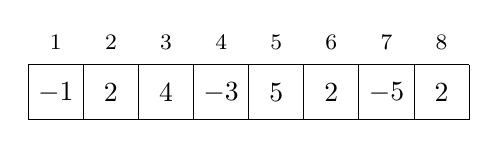
\begin{tikzpicture}[scale=0.7]
\draw (0,0) grid (8,1);

\node at (0.5,0.5) {$-1$};
\node at (1.5,0.5) {$2$};
\node at (2.5,0.5) {$4$};
\node at (3.5,0.5) {$-3$};
\node at (4.5,0.5) {$5$};
\node at (5.5,0.5) {$2$};
\node at (6.5,0.5) {$-5$};
\node at (7.5,0.5) {$2$};

\footnotesize
\node at (0.5,1.4) {$1$};
\node at (1.5,1.4) {$2$};
\node at (2.5,1.4) {$3$};
\node at (3.5,1.4) {$4$};
\node at (4.5,1.4) {$5$};
\node at (5.5,1.4) {$6$};
\node at (6.5,1.4) {$7$};
\node at (7.5,1.4) {$8$};
\end{tikzpicture}
\end{center}
\begin{samepage}
the following subarray produces the maximum sum $10$:
\begin{center}
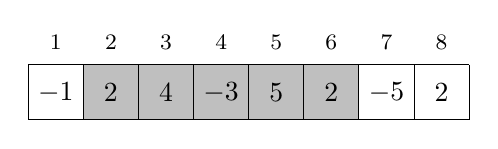
\begin{tikzpicture}[scale=0.7]
\fill[color=lightgray] (1,0) rectangle (6,1);
\draw (0,0) grid (8,1);

\node at (0.5,0.5) {$-1$};
\node at (1.5,0.5) {$2$};
\node at (2.5,0.5) {$4$};
\node at (3.5,0.5) {$-3$};
\node at (4.5,0.5) {$5$};
\node at (5.5,0.5) {$2$};
\node at (6.5,0.5) {$-5$};
\node at (7.5,0.5) {$2$};

\footnotesize
\node at (0.5,1.4) {$1$};
\node at (1.5,1.4) {$2$};
\node at (2.5,1.4) {$3$};
\node at (3.5,1.4) {$4$};
\node at (4.5,1.4) {$5$};
\node at (5.5,1.4) {$6$};
\node at (6.5,1.4) {$7$};
\node at (7.5,1.4) {$8$};
\end{tikzpicture}
\end{center}
\end{samepage}

\subsubsection{Algorithm 1}

A straightforward algorithm to the problem
is to go through all possible ways to
select a subarray, calculate the sum of
numbers in each subarray and maintain
the maximum sum.
The following code implements this algorithm:

\begin{lstlisting}
int p = 0;
for (int a = 1; a <= n; a++) {
    for (int b = a; b <= n; b++) {
        int s = 0;
        for (int c = a; c <= b; c++) {
            s += x[c];
        }
        p = max(p,s);
    }
}
cout << p << "\n";
\end{lstlisting}

The code assumes that the numbers are stored in an array \texttt{x}
with indices $1 \ldots n$.
The variables $a$ and $b$ determine the first and last
number in the subarray,
and the sum of the numbers is calculated to the variable $s$.
The variable $p$ contains the maximum sum found during the search.

The time complexity of the algorithm is $O(n^3)$,
because it consists of three nested loops and
each loop contains $O(n)$ steps.

\subsubsection{Algorithm 2}

It is easy to make the first algorithm more efficient
by removing one loop from it.
This is possible by calculating the sum at the same
time when the right end of the subarray moves.
The result is the following code:

\begin{lstlisting}
int p = 0;
for (int a = 1; a <= n; a++) {
    int s = 0;
    for (int b = a; b <= n; b++) {
        s += x[b];
        p = max(p,s);
    }
}
cout << p << "\n";
\end{lstlisting}
After this change, the time complexity is $O(n^2)$.

\subsubsection{Algorithm 3}

Surprisingly, it is possible to solve the problem
in $O(n)$ time, which means that we can remove
one more loop.
The idea is to calculate for each array position
the maximum sum of a subarray that ends at that position.
After this, the answer for the problem is the
maximum of those sums.

Condider the subproblem of finding the maximum-sum subarray
that ends at position $k$.
There are two possibilities:
\begin{enumerate}
\item The subarray only contains the element at position $k$.
\item The subarray consists of a subarray that ends
at position $k-1$, followed by the element at position $k$.
\end{enumerate}

Our goal is to find a subarray with maximum sum,
so in case 2 the subarray that ends at position $k-1$
should also have the maximum sum.
Thus, we can solve the problem efficiently
when we calculate the maximum subarray sum
for each ending position from left to right.

The following code implements the algorithm:
\begin{lstlisting}
int p = 0, s = 0;
for (int k = 1; k <= n; k++) {
    s = max(x[k],s+x[k]);
    p = max(p,s);
}
cout << p << "\n";
\end{lstlisting}

The algorithm only contains one loop
that goes through the input,
so the time complexity is $O(n)$.
This is also the best possible time complexity,
because any algorithm for the problem
has to examine all array elements at least once.

\subsubsection{Efficiency comparison}

It is interesting to study how efficient 
algorithms are in practice.
The following table shows the running times
of the above algorithms for different
values of $n$ in a modern computer.

In each test, the input was generated randomly.
The time needed for reading the input was not
measured.

\begin{center}
\begin{tabular}{rrrr}
array size $n$ & algorithm 1 & algorithm 2 & algorithm 3 \\
\hline
$10^2$ & $0{,}0$ s & $0{,}0$ s & $0{,}0$ s \\
$10^3$ & $0{,}1$ s & $0{,}0$ s & $0{,}0$ s \\
$10^4$ & > $10,0$ s & $0{,}1$ s & $0{,}0$ s \\
$10^5$ & > $10,0$ s & $5{,}3$ s & $0{,}0$ s \\
$10^6$ & > $10,0$ s & > $10,0$ s & $0{,}0$ s \\
$10^7$ & > $10,0$ s & > $10,0$ s & $0{,}0$ s \\
\end{tabular}
\end{center}

The comparison shows that all algorithms
are efficient when the input size is small,
but larger inputs bring out remarkable
differences in running times of the algorithms.
The $O(n^3)$ time algorithm 1 becomes slow
when $n=10^4$, and the $O(n^2)$ time algorithm 2
becomes slow when $n=10^5$.
Only the $O(n)$ time algorithm 3 processes
even the largest inputs instantly.

\chapter{Sorting}

\index{sorting}

\key{Sorting}
is a fundamental algorithm design problem.
In addition,
many efficient algorithms
use sorting as a subroutine,
because it is often easier to process
data if the elements are in a sorted order.

For example, the question ''does the array contain
two equal elements?'' is easy to solve using sorting.
If the array contains two equal elements,
they will be next to each other after sorting,
so it is easy to find them.
Also the question ''what is the most frequent element
in the array?'' can be solved similarly.

There are many algorithms for sorting, that are
also good examples of algorithm design techniques.
The efficient general sorting algorithms
work in $O(n \log n)$ time,
and many algorithms that use sorting
as a subroutine also
have this time complexity.

\section{Sorting theory}

The basic problem in sorting is as follows:
\begin{framed}
\noindent
Given an array that contains $n$ elements,
your task is to sort the elements
in increasing order.
\end{framed}
\noindent
For example, the array
\begin{center}
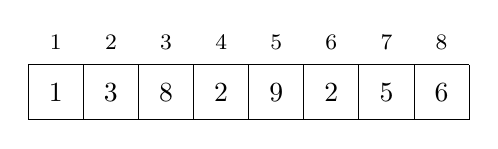
\begin{tikzpicture}[scale=0.7]
\draw (0,0) grid (8,1);
\node at (0.5,0.5) {$1$};
\node at (1.5,0.5) {$3$};
\node at (2.5,0.5) {$8$};
\node at (3.5,0.5) {$2$};
\node at (4.5,0.5) {$9$};
\node at (5.5,0.5) {$2$};
\node at (6.5,0.5) {$5$};
\node at (7.5,0.5) {$6$};

\footnotesize
\node at (0.5,1.4) {$1$};
\node at (1.5,1.4) {$2$};
\node at (2.5,1.4) {$3$};
\node at (3.5,1.4) {$4$};
\node at (4.5,1.4) {$5$};
\node at (5.5,1.4) {$6$};
\node at (6.5,1.4) {$7$};
\node at (7.5,1.4) {$8$};
\end{tikzpicture}
\end{center}
will be as follows after sorting:
\begin{center}
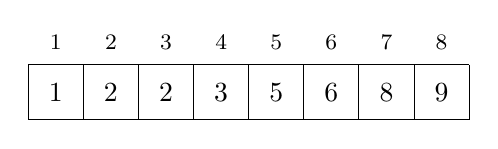
\begin{tikzpicture}[scale=0.7]
\draw (0,0) grid (8,1);
\node at (0.5,0.5) {$1$};
\node at (1.5,0.5) {$2$};
\node at (2.5,0.5) {$2$};
\node at (3.5,0.5) {$3$};
\node at (4.5,0.5) {$5$};
\node at (5.5,0.5) {$6$};
\node at (6.5,0.5) {$8$};
\node at (7.5,0.5) {$9$};

\footnotesize
\node at (0.5,1.4) {$1$};
\node at (1.5,1.4) {$2$};
\node at (2.5,1.4) {$3$};
\node at (3.5,1.4) {$4$};
\node at (4.5,1.4) {$5$};
\node at (5.5,1.4) {$6$};
\node at (6.5,1.4) {$7$};
\node at (7.5,1.4) {$8$};
\end{tikzpicture}
\end{center}

\subsubsection{$O(n^2)$ algorithms}

\index{bubble sort}

Simple algorithms for sorting an array
work in $O(n^2)$ time.
Such algorithms are short and usually
consist of two nested loops.
A famous $O(n^2)$ time sorting algorithm
is \key{bubble sort} where the elements
''bubble'' in the array according to their values.

Bubble sort consists of $n-1$ rounds.
On each round, the algorithm iterates through
the elements in the array.
Whenever two consecutive elements are found
that are not in correct order,
the algorithm swaps them.
The algorithm can be implemented as follows
for array
$\texttt{t}[1],\texttt{t}[2],\ldots,\texttt{t}[n]$:
\begin{lstlisting}
for (int i = 1; i <= n; i++) {
    for (int j = 1; j <= n-i; j++) {
        if (t[j] > t[j+1]) swap(t[j],t[j+1]);
    }
}
\end{lstlisting}

After the first round of the algorithm,
the largest element will be in the correct position,
and in general, after $k$ rounds, the $k$ largest
elements will be in the correct positions.
Thus, after $n$ rounds, the whole array
will be sorted.

For example, in the array

\begin{center}
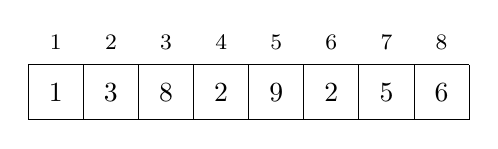
\begin{tikzpicture}[scale=0.7]
\draw (0,0) grid (8,1);

\node at (0.5,0.5) {$1$};
\node at (1.5,0.5) {$3$};
\node at (2.5,0.5) {$8$};
\node at (3.5,0.5) {$2$};
\node at (4.5,0.5) {$9$};
\node at (5.5,0.5) {$2$};
\node at (6.5,0.5) {$5$};
\node at (7.5,0.5) {$6$};

\footnotesize
\node at (0.5,1.4) {$1$};
\node at (1.5,1.4) {$2$};
\node at (2.5,1.4) {$3$};
\node at (3.5,1.4) {$4$};
\node at (4.5,1.4) {$5$};
\node at (5.5,1.4) {$6$};
\node at (6.5,1.4) {$7$};
\node at (7.5,1.4) {$8$};
\end{tikzpicture}
\end{center}

\noindent
the first round of bubble sort swaps elements
as follows:

\begin{center}
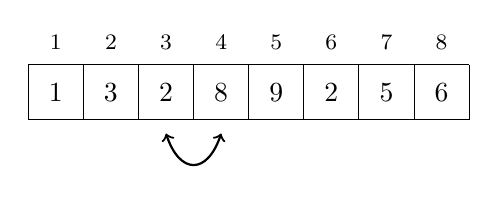
\begin{tikzpicture}[scale=0.7]
\draw (0,0) grid (8,1);
\node at (0.5,0.5) {$1$};
\node at (1.5,0.5) {$3$};
\node at (2.5,0.5) {$2$};
\node at (3.5,0.5) {$8$};
\node at (4.5,0.5) {$9$};
\node at (5.5,0.5) {$2$};
\node at (6.5,0.5) {$5$};
\node at (7.5,0.5) {$6$};

\draw[thick,<->] (3.5,-0.25) .. controls (3.25,-1.00) and (2.75,-1.00) .. (2.5,-0.25);

\footnotesize
\node at (0.5,1.4) {$1$};
\node at (1.5,1.4) {$2$};
\node at (2.5,1.4) {$3$};
\node at (3.5,1.4) {$4$};
\node at (4.5,1.4) {$5$};
\node at (5.5,1.4) {$6$};
\node at (6.5,1.4) {$7$};
\node at (7.5,1.4) {$8$};
\end{tikzpicture}
\end{center}

\begin{center}
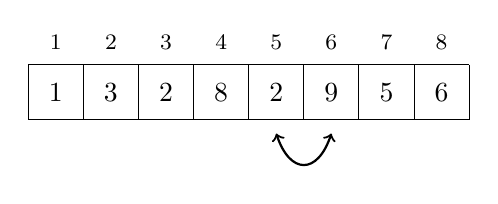
\begin{tikzpicture}[scale=0.7]
\draw (0,0) grid (8,1);
\node at (0.5,0.5) {$1$};
\node at (1.5,0.5) {$3$};
\node at (2.5,0.5) {$2$};
\node at (3.5,0.5) {$8$};
\node at (4.5,0.5) {$2$};
\node at (5.5,0.5) {$9$};
\node at (6.5,0.5) {$5$};
\node at (7.5,0.5) {$6$};

\draw[thick,<->] (5.5,-0.25) .. controls (5.25,-1.00) and (4.75,-1.00) .. (4.5,-0.25);


\footnotesize
\node at (0.5,1.4) {$1$};
\node at (1.5,1.4) {$2$};
\node at (2.5,1.4) {$3$};
\node at (3.5,1.4) {$4$};
\node at (4.5,1.4) {$5$};
\node at (5.5,1.4) {$6$};
\node at (6.5,1.4) {$7$};
\node at (7.5,1.4) {$8$};
\end{tikzpicture}
\end{center}

\begin{center}
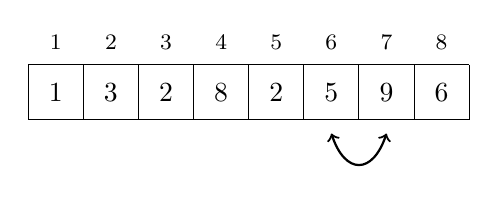
\begin{tikzpicture}[scale=0.7]
\draw (0,0) grid (8,1);
\node at (0.5,0.5) {$1$};
\node at (1.5,0.5) {$3$};
\node at (2.5,0.5) {$2$};
\node at (3.5,0.5) {$8$};
\node at (4.5,0.5) {$2$};
\node at (5.5,0.5) {$5$};
\node at (6.5,0.5) {$9$};
\node at (7.5,0.5) {$6$};

\draw[thick,<->] (6.5,-0.25) .. controls (6.25,-1.00) and (5.75,-1.00) .. (5.5,-0.25);


\footnotesize
\node at (0.5,1.4) {$1$};
\node at (1.5,1.4) {$2$};
\node at (2.5,1.4) {$3$};
\node at (3.5,1.4) {$4$};
\node at (4.5,1.4) {$5$};
\node at (5.5,1.4) {$6$};
\node at (6.5,1.4) {$7$};
\node at (7.5,1.4) {$8$};
\end{tikzpicture}
\end{center}

\begin{center}
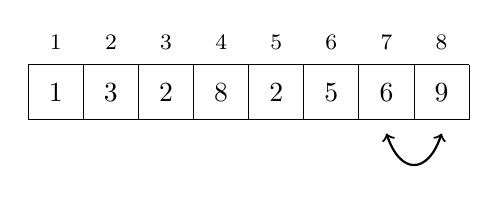
\begin{tikzpicture}[scale=0.7]
\draw (0,0) grid (8,1);
\node at (0.5,0.5) {$1$};
\node at (1.5,0.5) {$3$};
\node at (2.5,0.5) {$2$};
\node at (3.5,0.5) {$8$};
\node at (4.5,0.5) {$2$};
\node at (5.5,0.5) {$5$};
\node at (6.5,0.5) {$6$};
\node at (7.5,0.5) {$9$};

\draw[thick,<->] (7.5,-0.25) .. controls (7.25,-1.00) and (6.75,-1.00) .. (6.5,-0.25);

\footnotesize
\node at (0.5,1.4) {$1$};
\node at (1.5,1.4) {$2$};
\node at (2.5,1.4) {$3$};
\node at (3.5,1.4) {$4$};
\node at (4.5,1.4) {$5$};
\node at (5.5,1.4) {$6$};
\node at (6.5,1.4) {$7$};
\node at (7.5,1.4) {$8$};
\end{tikzpicture}
\end{center}

\subsubsection{Inversions}

\index{inversion}

Bubble sort is an example of a sorting
algorithm that always swaps consecutive
elements in the array.
It turns out that the time complexity
of such an algorithm is \emph{always}
at least $O(n^2)$ because in the worst case,
$O(n^2)$ swaps are required for sorting the array.

A useful concept when analyzing sorting
algorithms is an \key{inversion}:
a pair of elements
$(\texttt{t}[a],\texttt{t}[b])$
in the array such that
$a<b$ and $\texttt{t}[a]>\texttt{t}[b]$,
i.e., the elements are in the wrong order.
For example, in the array
\begin{center}
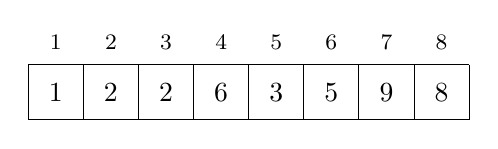
\begin{tikzpicture}[scale=0.7]
\draw (0,0) grid (8,1);
\node at (0.5,0.5) {$1$};
\node at (1.5,0.5) {$2$};
\node at (2.5,0.5) {$2$};
\node at (3.5,0.5) {$6$};
\node at (4.5,0.5) {$3$};
\node at (5.5,0.5) {$5$};
\node at (6.5,0.5) {$9$};
\node at (7.5,0.5) {$8$};

\footnotesize
\node at (0.5,1.4) {$1$};
\node at (1.5,1.4) {$2$};
\node at (2.5,1.4) {$3$};
\node at (3.5,1.4) {$4$};
\node at (4.5,1.4) {$5$};
\node at (5.5,1.4) {$6$};
\node at (6.5,1.4) {$7$};
\node at (7.5,1.4) {$8$};
\end{tikzpicture}
\end{center}
the inversions are $(6,3)$, $(6,5)$ and $(9,8)$.
The number of inversions indicates
how much work is needed to sort the array.
An array is completely sorted when
there are no inversions.
On the other hand, if the array elements
are in the reverse order,
the number of inversions is the largest possible:
\[1+2+\cdots+(n-1)=\frac{n(n-1)}{2} = O(n^2)\]

Swapping a pair of consecutive elements that are
in the wrong order removes exactly one inversion
from the array.
Hence, if a sorting algorithm can only
swap consecutive elements, each swap removes
at most one inversion and the time complexity
of the algorithm is at least $O(n^2)$.

\subsubsection{$O(n \log n)$ algorithms}

\index{merge sort}

It is possible to sort an array efficiently
in $O(n \log n)$ time using algorithms
that are not limited to swapping consecutive elements.
One such algorithm is \key{mergesort}
that is based on recursion.

Mergesort sorts a subarray \texttt{t}$[a,b]$ as follows:

\begin{enumerate}
\item If $a=b$, do not do anything because the subarray is already sorted.
\item Calculate the index of the middle element: $k=\lfloor (a+b)/2 \rfloor$.
\item Recursively sort the subarray \texttt{t}$[a,k]$.
\item Recursively sort the subarray \texttt{t}$[k+1,b]$.
\item \emph{Merge} the sorted subarrays \texttt{t}$[a,k]$ and \texttt{t}$[k+1,b]$
into a sorted subarray \texttt{t}$[a,b]$.
\end{enumerate}

Mergesort is an efficient algorithm because it
halves the size of the subarray at each step.
The recursion consists of $O(\log n)$ levels,
and processing each level takes $O(n)$ time.
Merging the subarrays \texttt{t}$[a,k]$ and \texttt{t}$[k+1,b]$
is possible in linear time because they are already sorted.

For example, consider sorting the following array:
\begin{center}
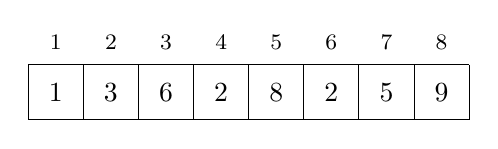
\begin{tikzpicture}[scale=0.7]
\draw (0,0) grid (8,1);
\node at (0.5,0.5) {$1$};
\node at (1.5,0.5) {$3$};
\node at (2.5,0.5) {$6$};
\node at (3.5,0.5) {$2$};
\node at (4.5,0.5) {$8$};
\node at (5.5,0.5) {$2$};
\node at (6.5,0.5) {$5$};
\node at (7.5,0.5) {$9$};

\footnotesize
\node at (0.5,1.4) {$1$};
\node at (1.5,1.4) {$2$};
\node at (2.5,1.4) {$3$};
\node at (3.5,1.4) {$4$};
\node at (4.5,1.4) {$5$};
\node at (5.5,1.4) {$6$};
\node at (6.5,1.4) {$7$};
\node at (7.5,1.4) {$8$};
\end{tikzpicture}
\end{center}

The array will be divided into two subarrays
as follows:
\begin{center}
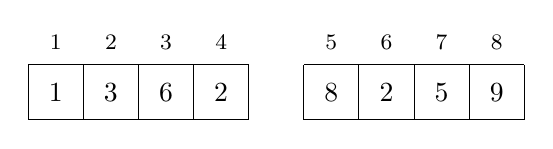
\begin{tikzpicture}[scale=0.7]
\draw (0,0) grid (4,1);
\draw (5,0) grid (9,1);

\node at (0.5,0.5) {$1$};
\node at (1.5,0.5) {$3$};
\node at (2.5,0.5) {$6$};
\node at (3.5,0.5) {$2$};

\node at (5.5,0.5) {$8$};
\node at (6.5,0.5) {$2$};
\node at (7.5,0.5) {$5$};
\node at (8.5,0.5) {$9$};

\footnotesize
\node at (0.5,1.4) {$1$};
\node at (1.5,1.4) {$2$};
\node at (2.5,1.4) {$3$};
\node at (3.5,1.4) {$4$};
\node at (5.5,1.4) {$5$};
\node at (6.5,1.4) {$6$};
\node at (7.5,1.4) {$7$};
\node at (8.5,1.4) {$8$};

\end{tikzpicture}
\end{center}

Then, the subarrays will be sorted recursively
as follows:
\begin{center}
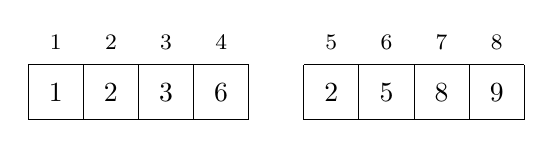
\begin{tikzpicture}[scale=0.7]
\draw (0,0) grid (4,1);
\draw (5,0) grid (9,1);

\node at (0.5,0.5) {$1$};
\node at (1.5,0.5) {$2$};
\node at (2.5,0.5) {$3$};
\node at (3.5,0.5) {$6$};

\node at (5.5,0.5) {$2$};
\node at (6.5,0.5) {$5$};
\node at (7.5,0.5) {$8$};
\node at (8.5,0.5) {$9$};

\footnotesize
\node at (0.5,1.4) {$1$};
\node at (1.5,1.4) {$2$};
\node at (2.5,1.4) {$3$};
\node at (3.5,1.4) {$4$};
\node at (5.5,1.4) {$5$};
\node at (6.5,1.4) {$6$};
\node at (7.5,1.4) {$7$};
\node at (8.5,1.4) {$8$};
\end{tikzpicture}
\end{center}

Finally, the algorithm merges the sorted
subarrays and creates the final sorted array:
\begin{center}
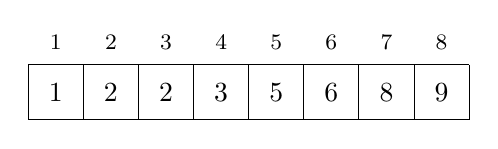
\begin{tikzpicture}[scale=0.7]
\draw (0,0) grid (8,1);
\node at (0.5,0.5) {$1$};
\node at (1.5,0.5) {$2$};
\node at (2.5,0.5) {$2$};
\node at (3.5,0.5) {$3$};
\node at (4.5,0.5) {$5$};
\node at (5.5,0.5) {$6$};
\node at (6.5,0.5) {$8$};
\node at (7.5,0.5) {$9$};

\footnotesize
\node at (0.5,1.4) {$1$};
\node at (1.5,1.4) {$2$};
\node at (2.5,1.4) {$3$};
\node at (3.5,1.4) {$4$};
\node at (4.5,1.4) {$5$};
\node at (5.5,1.4) {$6$};
\node at (6.5,1.4) {$7$};
\node at (7.5,1.4) {$8$};
\end{tikzpicture}
\end{center}

\subsubsection{Sorting lower bound}

Is it possible to sort an array faster
than in $O(n \log n)$ time?
It turns out that this is \emph{not} possible
when we restrict ourselves to sorting algorithms
that are based on comparing array elements.

The lower bound for the time complexity
can be proved by examining the sorting
as a process where each comparison of two elements
gives more information about the contents of the array.
The process creates the following tree:

\begin{center}
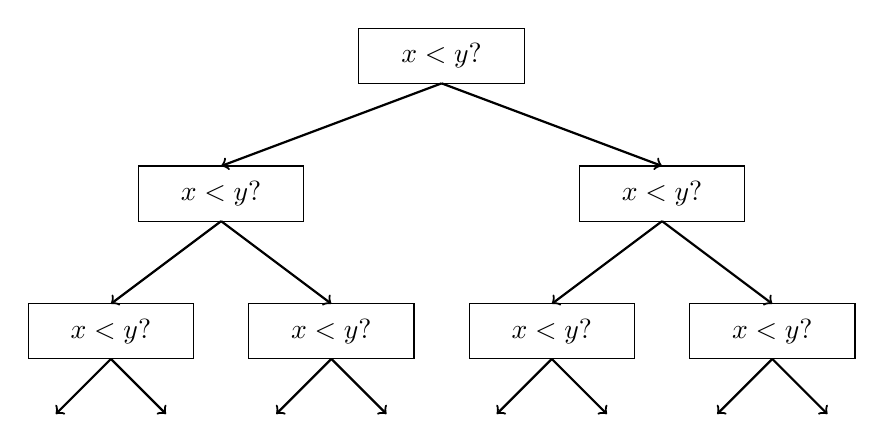
\begin{tikzpicture}[scale=0.7]
\draw (0,0) rectangle (3,1);
\node at (1.5,0.5) {$x < y?$};

\draw[thick,->] (1.5,0) -- (-2.5,-1.5);
\draw[thick,->] (1.5,0) -- (5.5,-1.5);

\draw (-4,-2.5) rectangle (-1,-1.5);
\draw (4,-2.5) rectangle (7,-1.5);
\node at (-2.5,-2) {$x < y?$};
\node at (5.5,-2) {$x < y?$};

\draw[thick,->] (-2.5,-2.5) -- (-4.5,-4);
\draw[thick,->] (-2.5,-2.5) -- (-0.5,-4);
\draw[thick,->] (5.5,-2.5) -- (3.5,-4);
\draw[thick,->] (5.5,-2.5) -- (7.5,-4);

\draw (-6,-5) rectangle (-3,-4);
\draw (-2,-5) rectangle (1,-4);
\draw (2,-5) rectangle (5,-4);
\draw (6,-5) rectangle (9,-4);
\node at (-4.5,-4.5) {$x < y?$};
\node at (-0.5,-4.5) {$x < y?$};
\node at (3.5,-4.5) {$x < y?$};
\node at (7.5,-4.5) {$x < y?$};

\draw[thick,->] (-4.5,-5) -- (-5.5,-6);
\draw[thick,->] (-4.5,-5) -- (-3.5,-6);
\draw[thick,->] (-0.5,-5) -- (0.5,-6);
\draw[thick,->] (-0.5,-5) -- (-1.5,-6);
\draw[thick,->] (3.5,-5) -- (2.5,-6);
\draw[thick,->] (3.5,-5) -- (4.5,-6);
\draw[thick,->] (7.5,-5) -- (6.5,-6);
\draw[thick,->] (7.5,-5) -- (8.5,-6);
\end{tikzpicture}
\end{center}

Here ''$x<y?$'' means that some elements
$x$ and $y$ are compared.
If $x<y$, the process continues to the left,
and otherwise to the right.
The results of the process are the possible
ways to sort the array, a total of $n!$ ways.
For this reason, the height of the tree
must be at least
\[ \log_2(n!) = \log_2(1)+\log_2(2)+\cdots+\log_2(n).\]
We get an lower bound for this sum
by choosing last $n/2$ elements and
changing the value of each element to $\log_2(n/2)$.
This yields an estimate
\[ \log_2(n!) \ge (n/2) \cdot \log_2(n/2),\]
so the height of the tree and the minimum
possible number of steps in a sorting
algorithm in the worst case
is at least $n \log n$.

\subsubsection{Counting sort}

\index{counting sort}

The lower bound $n \log n$ does not apply to
algorithms that do not compare array elements
but use some other information.
An example of such an algorithm is
\key{counting sort} that sorts an array in
$O(n)$ time assuming that every element in the array
is an integer between $0 \ldots c$ where $c$
is a small constant.

The algorithm creates a \emph{bookkeeping} array
whose indices are elements in the original array.
The algorithm iterates through the original array
and calculates how many times each element
appears in the array.

For example, the array
\begin{center}
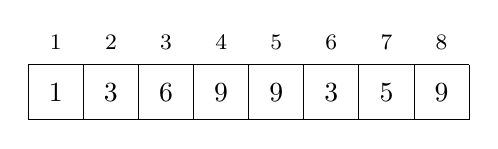
\begin{tikzpicture}[scale=0.7]
\draw (0,0) grid (8,1);
\node at (0.5,0.5) {$1$};
\node at (1.5,0.5) {$3$};
\node at (2.5,0.5) {$6$};
\node at (3.5,0.5) {$9$};
\node at (4.5,0.5) {$9$};
\node at (5.5,0.5) {$3$};
\node at (6.5,0.5) {$5$};
\node at (7.5,0.5) {$9$};

\footnotesize
\node at (0.5,1.4) {$1$};
\node at (1.5,1.4) {$2$};
\node at (2.5,1.4) {$3$};
\node at (3.5,1.4) {$4$};
\node at (4.5,1.4) {$5$};
\node at (5.5,1.4) {$6$};
\node at (6.5,1.4) {$7$};
\node at (7.5,1.4) {$8$};
\end{tikzpicture}
\end{center}
corresponds to the following bookkeeping array:
\begin{center}
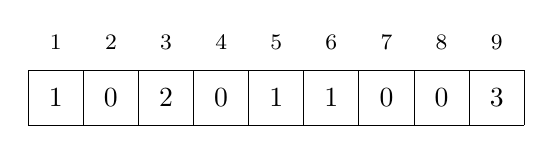
\begin{tikzpicture}[scale=0.7]
\draw (0,0) grid (9,1);
\node at (0.5,0.5) {$1$};
\node at (1.5,0.5) {$0$};
\node at (2.5,0.5) {$2$};
\node at (3.5,0.5) {$0$};
\node at (4.5,0.5) {$1$};
\node at (5.5,0.5) {$1$};
\node at (6.5,0.5) {$0$};
\node at (7.5,0.5) {$0$};
\node at (8.5,0.5) {$3$};

\footnotesize

\node at (0.5,1.5) {$1$};
\node at (1.5,1.5) {$2$};
\node at (2.5,1.5) {$3$};
\node at (3.5,1.5) {$4$};
\node at (4.5,1.5) {$5$};
\node at (5.5,1.5) {$6$};
\node at (6.5,1.5) {$7$};
\node at (7.5,1.5) {$8$};
\node at (8.5,1.5) {$9$};
\end{tikzpicture}
\end{center}

For example, the value at index 3
in the bookkeeping array is 2,
because the element 3 appears 2 times
in the original array (indices 2 and 6).

The construction of the bookkeeping array
takes $O(n)$ time. After this, the sorted array
can be created in $O(n)$ time because
the number of occurrences of each element can be retrieved
from the bookkeeping array.
Thus, the total time complexity of counting
sort is $O(n)$.

Counting sort is a very efficient algorithm
but it can only be used when the constant $c$
is so small that the array elements can
be used as indices in the bookkeeping array.

\section{Sorting in C++}

\index{sort@\texttt{sort}}

It is almost never a good idea to implement
an own sorting algorithm
in a contest, because there are good
implementations available in programming languages.
For example, the C++ standard library contains
the function \texttt{sort} that can be easily used for
sorting arrays and other data structures.

There are many benefits in using a library function.
First, it saves time because there is no need to
implement the function.
In addition, the library implementation is
certainly correct and efficient: it is not probable
that a home-made sorting function would be better.

In this section we will see how to use the
C++ \texttt{sort} function.
The following code sorts
a vector in increasing order:
\begin{lstlisting}
vector<int> v = {4,2,5,3,5,8,3};
sort(v.begin(),v.end());
\end{lstlisting}
After the sorting, the contents of the
vector will be
$[2,3,3,4,5,5,8]$.
The default sorting order is increasing,
but a reverse order is possible as follows:
\begin{lstlisting}
sort(v.rbegin(),v.rend());
\end{lstlisting}
A regular array can be sorted as follows:
\begin{lstlisting}
int n = 7; // array size
int t[] = {4,2,5,3,5,8,3};
sort(t,t+n);
\end{lstlisting}
The following code sorts the string \texttt{s}:
\begin{lstlisting}
string s = "monkey";
sort(s.begin(), s.end());
\end{lstlisting}
Sorting a string means that the characters
in the string are sorted.
For example, the string ''monkey'' becomes ''ekmnoy''.

\subsubsection{Comparison operator}

\index{comparison operator}

The function \texttt{sort} requires that
a \key{comparison operator} is defined for the data type
of the elements to be sorted.
During the sorting, this operator will be used
whenever it is needed to find out the order of two elements.

Most C++ data types have a built-in comparison operator
and elements of those types can be sorted automatically.
For example, numbers are sorted according to their values
and strings are sorted in alphabetical order.

\index{pair@\texttt{pair}}

Pairs (\texttt{pair}) are sorted primarily by the first
element (\texttt{first}).
However, if the first elements of two pairs are equal,
they are sorted by the second element (\texttt{second}):
\begin{lstlisting}
vector<pair<int,int>> v;
v.push_back({1,5});
v.push_back({2,3});
v.push_back({1,2});
sort(v.begin(), v.end());
\end{lstlisting}
After this, the order of the pairs is
$(1,2)$, $(1,5)$ and $(2,3)$.

\index{tuple@\texttt{tuple}}

Correspondingly, tuples (\texttt{tuple})
are sorted primarily by the first element,
secondarily by the second element, etc.:
\begin{lstlisting}
vector<tuple<int,int,int>> v;
v.push_back(make_tuple(2,1,4));
v.push_back(make_tuple(1,5,3));
v.push_back(make_tuple(2,1,3));
sort(v.begin(), v.end());
\end{lstlisting}
After this, the order of the tuples is
$(1,5,3)$, $(2,1,3)$ and $(2,1,4)$.

\subsubsection{User-defined structs}

User-defined structs do not have a comparison
operator automatically.
The operator should be defined inside
the struct as a function
\texttt{operator<}
whose parameter is another element of the same type.
The operator should return \texttt{true}
if the element is smaller than the parameter,
and \texttt{false} otherwise.

For example, the following struct \texttt{P}
contains the x and y coordinate of a point.
The comparison operator is defined so that
the points are sorted primarily by the x coordinate
and secondarily by the y coordinate.

\begin{lstlisting}
struct P {
    int x, y;
    bool operator<(const P &p) {
        if (x != p.x) return x < p.x;
        else return y < p.y;
    }
};
\end{lstlisting}

\subsubsection{Comparison function}

\index{comparison function}

It is also possible to give an external
\key{comparison function} to the \texttt{sort} function
as a callback function.
For example, the following comparison function
sorts strings primarily by length and secondarily
by alphabetical order:

\begin{lstlisting}
bool cmp(string a, string b) {
    if (a.size() != b.size()) return a.size() < b.size();
    return a < b;
}
\end{lstlisting}
Now a vector of strings can be sorted as follows:
\begin{lstlisting}
sort(v.begin(), v.end(), cmp);
\end{lstlisting}

\section{Binary search}

\index{binary search}

A general method for searching for an element
in an array is to use a \texttt{for} loop
that iterates through the elements in the array.
For example, the following code searches for
an element $x$ in the array \texttt{t}:

\begin{lstlisting}
for (int i = 1; i <= n; i++) {
    if (t[i] == x) // x found at index i
}
\end{lstlisting}

The time complexity of this approach is $O(n)$,
because in the worst case, it is needed to check
all elements in the array.
If the array can contain any elements,
this is also the best possible approach, because
there is no additional information available where
in the array we should search for the element $x$.

However, if the array is \emph{sorted},
the situation is different.
In this case it is possible to perform the
search much faster, because the order of the
elements in the array guides us.
The following \key{binary search} algorithm
efficiently searches for an element in a sorted array
in $O(\log n)$ time.

\subsubsection{Method 1}

The traditional way to implement binary search
resembles looking for a word in a dictionary.
At each step, the search halves the active region in the array, 
until the target element is found, or it turns out
that there is no such element.

First, the search checks the middle element in the array.
If the middle element is the target element,
the search terminates.
Otherwise, the search recursively continues
to the left or right half of the array,
depending on the value of the middle element.

The above idea can be implemented as follows:
\begin{lstlisting}
int a = 1, b = n;
while (a <= b) {
    int k = (a+b)/2;
    if (t[k] == x) // x found at index k
    if (t[k] > x) b = k-1;
    else a = k+1;
}
\end{lstlisting}

The algorithm maintains a range $a \ldots b$
that corresponds to the active region in the array.
Initially, the range is $1 \ldots n$, the whole array.
The algorithm halves the size of the range at each step,
so the time complexity is $O(\log n)$.

\subsubsection{Method 2}

An alternative method for implementing binary search
is based on an efficient way to iterate through
the elements in the array.
The idea is to make jumps and slow the speed
when we get closer to the target element.

The search goes through the array from left to
right, and the initial jump length is $n/2$.
At each step, the jump length will be halved:
first $n/4$, then $n/8$, $n/16$, etc., until
finally the length is 1.
After the jumps, either the target element has
been found or we know that it does not appear in the array.

The following code implements the above idea:
\begin{lstlisting}
int k = 1;
for (int b = n/2; b >= 1; b /= 2) {
    while (k+b <= n && t[k+b] <= x) k += b;
}
if (t[k] == x) // x was found at index k
\end{lstlisting}

The variables $k$ and $b$ contain the position
in the array and the jump length.
If the array contains the element $x$,
the index of the element will be in the variable $k$
after the search.
The time complexity of the algorithm is $O(\log n)$,
because the code in the \texttt{while} loop
is performed at most twice for each jump length.

\subsubsection{Finding the smallest solution}

In practice, it is seldom needed to implement
binary search for searching elements in an array,
because we can use the standard library instead.
For example, the C++ functions \texttt{lower\_bound}
and \texttt{upper\_bound} implement binary search,
and the data structure \texttt{set} maintains a
set of elements with $O(\log n)$ time operations.

However, an important use for binary search is
to find the position where the value of a function changes.
Suppose that we wish to find the smallest value $k$
that is a valid solution for a problem.
We are given a function $\texttt{ok}(x)$
that returns \texttt{true} if $x$ is a valid solution
and \texttt{false} otherwise.
In addition, we know that $\texttt{ok}(x)$ is \texttt{false}
when $x<k$ and \texttt{true} when $x \ge k$.
The situation looks as follows:

\begin{center}
\begin{tabular}{r|rrrrrrrr}
$x$ & 0 & 1 & $\cdots$ & $k-1$ & $k$ & $k+1$ & $\cdots$ \\
\hline
$\texttt{ok}(x)$ & \texttt{false} & \texttt{false}
& $\cdots$ & \texttt{false} & \texttt{true} & \texttt{true} & $\cdots$ \\
\end{tabular}
\end{center}

\noindent
The value $k$ can be found using binary search:

\begin{lstlisting}
int x = -1;
for (int b = z; b >= 1; b /= 2) {
    while (!ok(x+b)) x += b;
}
int k = x+1;
\end{lstlisting}

The search finds the largest value of $x$ for which
$\texttt{ok}(x)$ is \texttt{false}.
Thus, the next value $k=x+1$
is the smallest possible value for which
$\texttt{ok}(k)$ is \texttt{true}.
The initial jump length $z$ has to be
large enough, for example some value
for which we know beforehand that $\texttt{ok}(z)$ is \texttt{true}.

The algorithm calls the function \texttt{ok}
$O(\log z)$ times, so the total time complexity
depends on the function \texttt{ok}.
For example, if the function works in $O(n)$ time,
the total time complexity is $O(n \log z)$.

\subsubsection{Finding the maximum value}

Binary search can also be used to find
the maximum value for a function that is
first increasing and then decreasing.
Our task is to find a value $k$ such that

\begin{itemize}
\item
$f(x)<f(x+1)$ when $x<k$, and
\item
$f(x)>f(x+1)$ when $x \ge k$.
\end{itemize}

The idea is to use binary search
for finding the largest value of $x$
for which $f(x)<f(x+1)$.
This implies that $k=x+1$
because $f(x+1)>f(x+2)$.
The following code implements the search: 

\begin{lstlisting}
int x = -1;
for (int b = z; b >= 1; b /= 2) {
    while (f(x+b) < f(x+b+1)) x += b;
}
int k = x+1;
\end{lstlisting}

Note that unlike in the standard binary search,
here it is not allowed that consecutive values
of the function are equal.
In this case it would not be possible to know
how to continue the search.
\chapter{Data structures}

\index{tietorakenne@tietorakenne}

\key{Tietorakenne}
on tapa säilyttää tietoa tietokoneen muistissa.
Sopivan tietorakenteen valinta on tärkeää,
koska kullakin rakenteella on omat
vahvuutensa ja heikkoutensa.
Tietorakenteen valinnassa oleellinen kysymys on,
mitkä operaatiot rakenne toteuttaa tehokkaasti.

Tämä luku esittelee keskeisimmät
C++:n standardikirjaston tietorakenteet.
Valmiita tietorakenteita kannattaa käyttää
aina kun mahdollista, 
koska se säästää paljon aikaa toteutuksessa.
Myöhemmin kirjassa tutustumme erikoisempiin
rakenteisiin, joita ei ole valmiina C++:ssa.

\section{Dynaaminen taulukko}

\index{vektori@vektori}
\index{vector@\texttt{vector}}

\key{Dynaaminen taulukko} on taulukko,
jonka kokoa voi muuttaa
ohjelman suorituksen aikana.
C++:n tavallisin dynaaminen taulukko
on \key{vektori} (\texttt{vector}).
Sitä voi käyttää hyvin samalla tavalla
kuin tavallista taulukkoa.

Seuraava koodi luo tyhjän vektorin
ja lisää siihen kolme lukua:

\begin{lstlisting}
vector<int> v;
v.push_back(3); // [3]
v.push_back(2); // [3,2]
v.push_back(5); // [3,2,5]
\end{lstlisting}

Tämän jälkeen vektorin sisältöä voi käsitellä taulukon tavoin:

\begin{lstlisting}
cout << v[0] << "\n"; // 3
cout << v[1] << "\n"; // 2
cout << v[2] << "\n"; // 5
\end{lstlisting}

Funktio \texttt{size} kertoo, montako alkiota vektorissa on.
Seuraava koodi käy läpi ja tulostaa kaikki vektorin alkiot:

\begin{lstlisting}
for (int i = 0; i < v.size(); i++) {
    cout << v[i] << "\n";
}
\end{lstlisting}

\begin{samepage}
Vektorin voi käydä myös läpi lyhyemmin näin:

\begin{lstlisting}
for (auto x : v) {
    cout << x << "\n";
}
\end{lstlisting}
\end{samepage}

Funktio \texttt{back} hakee vektorin viimeisen alkion,
ja funktio \texttt{pop\_back} poistaa vektorin
viimeisen alkion:

\begin{lstlisting}
vector<int> v;
v.push_back(5);
v.push_back(2);
cout << v.back() << "\n"; // 2
v.pop_back();
cout << v.back() << "\n"; // 5
\end{lstlisting}

Vektorin sisällön voi antaa myös sen luonnissa:

\begin{lstlisting}
vector<int> v = {2,4,2,5,1};
\end{lstlisting}

Kolmas tapa luoda vektori on ilmoittaa
vektorin koko ja alkuarvo:

\begin{lstlisting}
// koko 10, alkuarvo 0
vector<int> v(10);
\end{lstlisting}
\begin{lstlisting}
// koko 10, alkuarvo 5
vector<int> v(10, 5);
\end{lstlisting}

Vektori on toteutettu sisäisesti tavallisena taulukkona.
Jos vektorin koko kasvaa ja taulukko jää liian pieneksi,
varataan uusi suurempi taulukko, johon kopioidaan
vektorin sisältö.
Näin tapahtuu kuitenkin niin harvoin, että vektorin
funktion \texttt{push\_back} aikavaativuus on
keskimäärin $O(1)$.

\index{merkkijono@merkkijono}
\index{string@\texttt{string}}

Myös \key{merkkijono} (\texttt{string}) on dynaaminen taulukko,
jota pystyy käsittelemään lähes samaan
tapaan kuin vektoria.
Merkkijonon käsittelyyn liittyy lisäksi erikoissyntaksia
ja funktioita, joita ei ole muissa tietorakenteissa.
Merkkijonoja voi yhdistää toisiinsa \texttt{+}-merkin avulla.
Funktio $\texttt{substr}(k,x)$ erottaa merkkijonosta
osajonon, joka alkaa kohdasta $k$ ja jonka pituus on $x$.
Funktio $\texttt{find}(\texttt{t})$ etsii kohdan,
jossa osajono \texttt{t} esiintyy merkkijonossa.

Seuraava koodi esittelee merkkijonon käyttämistä:

\begin{lstlisting}
string a = "hatti";
string b = a+a;
cout << b << "\n"; // hattihatti
b[5] = 'v';
cout << b << "\n"; // hattivatti
string c = b.substr(3,4);
cout << c << "\n"; // tiva
\end{lstlisting}

\section{Joukkorakenne}

\index{joukko@joukko}
\index{set@\texttt{set}}
\index{unordered\_set@\texttt{unordered\_set}}

\key{Joukko} on tietorakenne,
joka sisältää kokoelman alkioita.
Joukon perusoperaatiot ovat alkion lisäys,
haku ja poisto.

C++ sisältää kaksi
toteutusta joukolle: \texttt{set} ja \texttt{unordered\_set}.
Rakenne \texttt{set} perustuu tasapainoiseen
binääripuuhun, ja sen operaatioiden aikavaativuus
on $O(\log n)$.
Rakenne \texttt{unordered\_set} pohjautuu hajautustauluun,
ja sen operaatioiden aikavaativuus on keskimäärin $O(1)$.

Usein on makuasia, kumpaa joukon toteutusta käyttää.
Rakenteen \texttt{set} etuna on, että se säilyttää
joukon alkioita järjestyksessä ja tarjoaa
järjestykseen liittyviä funktioita,
joita \texttt{unordered\_set} ei sisällä.
Toisaalta \texttt{unordered\_set} on usein nopeampi rakenne.

Seuraava koodi luo lukuja sisältävän joukon ja
esittelee sen käyttämistä.
Funktio \texttt{insert} lisää joukkoon alkion,
funktio \texttt{count} laskee alkion määrän joukossa
ja funktio \texttt{erase} poistaa alkion joukosta.

\begin{lstlisting}
set<int> s;
s.insert(3);
s.insert(2);
s.insert(5);
cout << s.count(3) << "\n"; // 1
cout << s.count(4) << "\n"; // 0
s.erase(3);
s.insert(4);
cout << s.count(3) << "\n"; // 0
cout << s.count(4) << "\n"; // 1
\end{lstlisting}

Joukkoa voi käsitellä muuten suunnilleen samalla tavalla
kuin vektoria, mutta joukkoa ei voi indeksoida
\texttt{[]}-merkinnällä.
Seuraava koodi luo joukon, tulostaa sen 
alkioiden määrän ja käy sitten läpi kaikki alkiot.
\begin{lstlisting}
set<int> s = {2,5,6,8};
cout << s.size() << "\n"; // 4
for (auto x : s) {
    cout << x << "\n";
}
\end{lstlisting}

Tärkeä joukon ominaisuus on,
että tietty alkio voi esiintyä siinä
enintään kerran.
Niinpä funktio \texttt{count} palauttaa aina
arvon 0 (alkiota ei ole joukossa) tai 1 (alkio on joukossa)
ja funktio \texttt{insert} ei lisää alkiota
uudestaan joukkoon, jos se on siellä valmiina.
Seuraava koodi havainnollistaa asiaa:

\begin{lstlisting}
set<int> s;
s.insert(5);
s.insert(5);
s.insert(5);
cout << s.count(5) << "\n"; // 1
\end{lstlisting}

\index{multiset@\texttt{multiset}}
\index{unordered\_multiset@\texttt{unordered\_multiset}}

C++ sisältää myös rakenteet
\texttt{multiset} ja \texttt{unordered\_multiset},
jotka toimivat muuten samalla tavalla kuin \texttt{set}
ja \texttt{unordered\_set},
mutta sama alkio voi esiintyä
monta kertaa joukossa.
Esimerkiksi seuraavassa koodissa
kaikki luvun 5 kopiot lisätään joukkoon:

\begin{lstlisting}
multiset<int> s;
s.insert(5);
s.insert(5);
s.insert(5);
cout << s.count(5) << "\n"; // 3
\end{lstlisting}
Funktio \texttt{erase} poistaa
kaikki alkion esiintymät
\texttt{multiset}-rakenteessa:
\begin{lstlisting}
s.erase(5);
cout << s.count(5) << "\n"; // 0
\end{lstlisting}
Usein kuitenkin tulisi poistaa
vain yksi esiintymä,
mikä onnistuu näin:
\begin{lstlisting}
s.erase(s.find(5));
cout << s.count(5) << "\n"; // 2
\end{lstlisting}

\section{Hakemisto}

\index{hakemisto@hakemisto}
\index{map@\texttt{map}}
\index{unordered\_map@\texttt{unordered\_map}}

\key{Hakemisto} on taulukon yleistys,
joka sisältää kokoelman avain-arvo-pareja.
Siinä missä taulukon avaimet ovat aina peräkkäiset
kokonaisluvut $0,1,\ldots,n-1$,
missä $n$ on taulukon koko,
hakemiston avaimet voivat
olla mitä tahansa tyyppiä
eikä niiden tarvitse olla peräkkäin.

C++ sisältää kaksi toteutusta hakemistolle
samaan tapaan kuin joukolle.
Rakenne
\texttt{map} perustuu
tasapainoiseen binääripuuhun ja sen
alkioiden käsittely vie aikaa $O(\log n)$,
kun taas rakenne
\texttt{unordered\_map} perustuu
hajautustauluun ja sen alkioiden
käsittely vie keskimäärin aikaa $O(1)$.

Seuraava koodi toteuttaa hakemiston,
jossa avaimet ovat merkkijonoja ja
arvot ovat kokonaislukuja:

\begin{lstlisting}
map<string,int> m;
m["apina"] = 4;
m["banaani"] = 3;
m["cembalo"] = 9;
cout << m["banaani"] << "\n"; // 3
\end{lstlisting}

Jos hakemistosta hakee avainta,
jota ei ole siinä,
avain lisätään hakemistoon
automaattisesti oletusarvolla.
Esimerkiksi seuraavassa koodissa
hakemistoon ilmestyy avain ''aybabtu'',
jonka arvona on 0:

\begin{lstlisting}
map<string,int> m;
cout << m["aybabtu"] << "\n"; // 0
\end{lstlisting}
Funktiolla \texttt{count} voi
tutkia, esiintyykö avain hakemistossa:
\begin{lstlisting}
if (m.count("aybabtu")) {
    cout << "avain on hakemistossa";
}
\end{lstlisting}
Seuraava koodi listaa hakemiston
kaikki avaimet ja arvot:
\begin{lstlisting}
for (auto x : m) {
    cout << x.first << " " << x.second << "\n";
}
\end{lstlisting}

\section{Iteraattorit ja välit}

\index{iteraattori@iteraattori}

Monet C++:n standardikirjaston funktiot
käsittelevät tietorakenteiden iteraattoreita
ja niiden määrittelemiä välejä.
\key{Iteraattori} on muuttuja,
joka osoittaa tiettyyn tietorakenteen alkioon.

Usein tarvittavat iteraattorit ovat \texttt{begin}
ja \texttt{end}, jotka rajaavat välin,
joka sisältää kaikki tietorakenteen alkiot.
Iteraattori \texttt{begin} osoittaa
tietorakenteen ensimmäiseen alkioon,
kun taas iteraattori \texttt{end} osoittaa
tietorakenteen viimeisen alkion jälkeiseen kohtaan.
Tilanne on siis tällainen:

\begin{center}
\begin{tabular}{llllllllll}
\{ & 3, & 4, & 6, & 8, & 12, & 13, & 14, & 17 & \} \\
& $\uparrow$ & & & & & & & & $\uparrow$ \\
& \multicolumn{3}{l}{\texttt{s.begin()}} & & & & & & \texttt{s.end()} \\
\end{tabular}
\end{center}

Huomaa epäsymmetria iteraattoreissa:
\texttt{s.begin()} osoittaa tietorakenteen alkioon,
kun taas \texttt{s.end()} osoittaa tietorakenteen ulkopuolelle.
Iteraattoreiden rajaama joukon väli on siis \emph{puoliavoin}.

\subsubsection{Välien käsittely}

Iteraattoreita tarvitsee
C++:n standardikirjaston funktioissa, jotka käsittelevät
tietorakenteen välejä.
Yleensä halutaan käsitellä tietorakenteiden kaikkia
alkioita, jolloin funktiolle annetaan
iteraattorit \texttt{begin} ja \texttt{end}.

Esimerkiksi seuraava koodi järjestää vektorin funktiolla \texttt{sort},
kääntää sitten alkioiden järjestyksen funktiolla \texttt{reverse}
ja sekoittaa lopuksi alkioiden järjestyksen funktiolla \texttt{random\_shuffle}.

\index{sort@\texttt{sort}}
\index{reverse@\texttt{reverse}}
\index{random\_shuffle@\texttt{random\_shuffle}}

\begin{lstlisting}
sort(v.begin(), v.end());
reverse(v.begin(), v.end());
random_shuffle(v.begin(), v.end());
\end{lstlisting}

Samoja funktioita voi myös käyttää tavallisen taulukon
yhteydessä, jolloin iteraattorin sijasta annetaan
osoitin taulukkoon:

\begin{lstlisting}
sort(t, t+n);
reverse(t, t+n);
random_shuffle(t, t+n);
\end{lstlisting}

\subsubsection{Joukon iteraattorit}

Iteraattoreita tarvitsee usein joukon
alkioiden käsittelyssä.
Seuraava koodi määrittelee iteraattorin
\texttt{it}, joka osoittaa joukon \texttt{s} alkuun:
\begin{lstlisting}
set<int>::iterator it = s.begin();
\end{lstlisting}
Koodin voi kirjoittaa myös lyhyemmin näin:
\begin{lstlisting}
auto it = s.begin();
\end{lstlisting}
Iteraattoria vastaavaan joukon alkioon
pääsee käsiksi \texttt{*}-merkinnällä.
Esimerkiksi seuraava koodi tulostaa
joukon ensimmäisen alkion:

\begin{lstlisting}
auto it = s.begin();
cout << *it << "\n";
\end{lstlisting}

Iteraattoria pystyy liikuttamaan
operaatioilla \texttt{++} (eteenpäin)
ja \texttt{---} (taaksepäin).
Tällöin iteraattori siirtyy seuraavaan
tai edelliseen alkioon joukossa.

Seuraava koodi tulostaa joukon kaikki alkiot:

\begin{lstlisting}
for (auto it = s.begin(); it != s.end(); it++) {
    cout << *it << "\n";
}
\end{lstlisting}
Seuraava koodi taas tulostaa joukon
viimeisen alkion:

\begin{lstlisting}
auto it = s.end();
it--;
cout << *it << "\n";
\end{lstlisting}
% Iteraattoria täytyi liikuttaa askel taaksepäin,
% koska se osoitti aluksi joukon viimeisen
% alkion jälkeiseen kohtaan.

Funktio $\texttt{find}(x)$ palauttaa iteraattorin
joukon alkioon, jonka arvo on $x$.
Poikkeuksena jos alkiota $x$ ei esiinny joukossa,
iteraattoriksi tulee \texttt{end}.

\begin{lstlisting}
auto it = s.find(x);
if (it == s.end()) cout << "x puuttuu joukosta";
\end{lstlisting}

Funktio $\texttt{lower\_bound}(x)$ palauttaa
iteraattorin joukon pienimpään alkioon,
joka on ainakin yhtä suuri kuin $x$.
Vastaavasti $\texttt{upper\_bound}(x)$ palauttaa
iteraattorin pienimpään alkioon,
joka on suurempi kuin $x$.
Jos tällaisia alkioita ei ole joukossa,
funktiot palauttavat arvon \texttt{end}.
Näitä funktioita ei voi käyttää
\texttt{unordered\_set}-rakenteessa,
joka ei pidä yllä alkioiden järjestystä.

\begin{samepage}
Esimerkiksi seuraava koodi etsii joukosta
alkion, joka on lähinnä lukua $x$:

\begin{lstlisting}
auto a = s.lower_bound(x);
if (a == s.begin() && a == s.end()) {
    cout << "joukko on tyhjä\n";
} else if (a == s.begin()) {
    cout << *a << "\n";
} else if (a == s.end()) {
    a--;
    cout << *a << "\n";
} else {
    auto b = a; b--;
    if (x-*b < *a-x) cout << *b << "\n";
    else cout << *a << "\n";
}
\end{lstlisting}

Koodi käy läpi mahdolliset tapaukset
iteraattorin \texttt{a} avulla.
Iteraattori
osoittaa aluksi pienimpään alkioon,
joka on ainakin yhtä suuri kuin $x$.
Jos \texttt{a} on samaan aikaan \texttt{begin}
ja \texttt{end}, joukko on tyhjä.
Muuten jos \texttt{a} on \texttt{begin},
sen osoittama alkio on $x$:ää lähin alkio.
Jos taas \texttt{a} on \texttt{end},
$x$:ää lähin alkio on joukon viimeinen alkio.
Jos mikään edellisistä tapauksista ei päde,
niin $x$:ää lähin alkio
on joko $a$:n osoittama alkio tai sitä edellinen alkio.
\end{samepage}

\section{Muita tietorakenteita}

\subsubsection{Bittijoukko}

\index{bittijoukko@bittijoukko}
\index{bitset@\texttt{bitset}}

\key{Bittijoukko} (\texttt{bitset}) on taulukko,
jonka jokaisen alkion arvo on 0 tai 1.
Esimerkiksi
seuraava koodi luo bittijoukon, jossa on 10 alkiota.
\begin{lstlisting}
bitset<10> s;
s[2] = 1;
s[5] = 1;
s[6] = 1;
s[8] = 1;
cout << s[4] << "\n"; // 0
cout << s[5] << "\n"; // 1
\end{lstlisting}

Bittijoukon etuna on, että se vie tavallista
taulukkoa vähemmän muistia,
koska jokainen alkio vie
vain yhden bitin muistia.
Esimerkiksi $n$ bitin tallentaminen
\texttt{int}-taulukkona vie $32n$
bittiä tilaa, mutta bittijoukkona
vain $n$ bittiä tilaa.
Lisäksi bittijoukon sisältöä
voi käsitellä tehokkaasti bittioperaatioilla,
minkä ansiosta sillä voi tehostaa algoritmeja.

Seuraava koodi näyttää toisen tavan
bittijoukon luomiseen:

\begin{lstlisting}
bitset<10> s(string("0010011010"));
cout << s[4] << "\n"; // 0
cout << s[5] << "\n"; // 1
\end{lstlisting}

Funktio \texttt{count} palauttaa
bittijoukon ykkösbittien määrän:

\begin{lstlisting}
bitset<10> s(string("0010011010"));
cout << s.count() << "\n"; // 4
\end{lstlisting}

Seuraava koodi näyttää esimerkkejä
bittioperaatioiden käyttämisestä:
\begin{lstlisting}
bitset<10> a(string("0010110110"));
bitset<10> b(string("1011011000"));
cout << (a&b) << "\n"; // 0010010000
cout << (a|b) << "\n"; // 1011111110
cout << (a^b) << "\n"; // 1001101110
\end{lstlisting}

\subsubsection{Pakka}

\index{pakka@pakka}
\index{deque@\texttt{deque}}

\key{Pakka} (\texttt{deque}) on dynaaminen taulukko,
jonka kokoa pystyy muuttamaan tehokkaasti
sekä alku- että loppupäässä.
Pakka sisältää vektorin tavoin
funktiot \texttt{push\_back}
ja \texttt{pop\_back}, mutta siinä on lisäksi myös funktiot
\texttt{push\_front} ja \texttt{pop\_front},
jotka käsittelevät taulukon alkua.

Seuraava koodi esittelee pakan käyttämistä:

\begin{lstlisting}
deque<int> d;
d.push_back(5); // [5]
d.push_back(2); // [5,2]
d.push_front(3); // [3,5,2]
d.pop_back(); // [3,5]
d.pop_front(); // [5]
\end{lstlisting}

Pakan sisäinen toteutus on monimutkaisempi kuin
vektorissa, minkä vuoksi se on
vektoria raskaampi rakenne.
Kuitenkin lisäyksen ja poiston
aikavaativuus on keskimäärin $O(1)$ molemmissa päissä.

\subsubsection{Pino}

\index{pino@pino}
\index{stack@\texttt{stack}}

\key{Pino} (\texttt{stack}) on tietorakenne,
joka tarjoaa kaksi $O(1)$-aikaista
operaatiota:
alkion lisäys pinon päälle ja alkion
poisto pinon päältä.
Pinossa ei ole mahdollista käsitellä muita
alkioita kuin pinon päällimmäistä alkiota.

Seuraava koodi esittelee pinon käyttämistä:

\begin{lstlisting}
stack<int> s;
s.push(3);
s.push(2);
s.push(5);
cout << s.top(); // 5
s.pop();
cout << s.top(); // 2
\end{lstlisting}
\subsubsection{Jono}

\index{jono@jono}
\index{queue@\texttt{queue}}

\key{Jono} (\texttt{queue}) on kuin pino,
mutta alkion lisäys tapahtuu jonon loppuun
ja alkion poisto tapahtuu jonon alusta.
Jonossa on mahdollista käsitellä vain
alussa ja lopussa olevaa alkiota.

Seuraava koodi esittelee jonon käyttämistä:

\begin{lstlisting}
queue<int> s;
s.push(3);
s.push(2);
s.push(5);
cout << s.front(); // 3
s.pop();
cout << s.front(); // 2
\end{lstlisting}
% 
% Huomaa, että rakenteiden \texttt{stack} ja \texttt{queue}
% sijasta voi aina käyttää rakenteita
% \texttt{vector} ja \texttt{deque}, joilla voi
% tehdä kaiken saman ja enemmän.
% Kuitenkin \texttt{stack} ja \texttt{queue} ovat
% kevyempiä ja hieman tehokkaampia rakenteita,
% jos niiden operaatiot riittävät algoritmin toteuttamiseen.

\subsubsection{Prioriteettijono}

\index{prioriteettijono@prioriteettijono}
\index{keko@keko}
\index{priority\_queue@\texttt{priority\_queue}}

\key{Prioriteettijono} (\texttt{priority\_queue})
pitää yllä joukkoa alkioista.
Sen operaatiot ovat alkion lisäys ja
jonon tyypistä riippuen joko
pienimmän alkion haku ja poisto tai
suurimman alkion haku ja poisto.
Lisäyksen ja poiston aikavaativuus on $O(\log n)$
ja haun aikavaativuus on $O(1)$.

Vaikka prioriteettijonon operaatiot
pystyy toteuttamaan myös \texttt{set}-ra\-ken\-teel\-la,
prioriteettijonon etuna on,
että sen kekoon perustuva sisäinen
toteutus on yksinkertaisempi
kuin \texttt{set}-rakenteen tasapainoinen binääripuu,
minkä vuoksi rakenne on kevyempi ja
operaatiot ovat tehokkaampia.

\begin{samepage}
C++:n prioriteettijono toimii oletuksena niin,
että alkiot ovat järjestyksessä suurimmasta pienimpään
ja jonosta pystyy hakemaan ja poistamaan suurimman alkion.
Seuraava koodi esittelee prioriteettijonon käyttämistä:

\begin{lstlisting}
priority_queue<int> q;
q.push(3);
q.push(5);
q.push(7);
q.push(2);
cout << q.top() << "\n"; // 7
q.pop();
cout << q.top() << "\n"; // 5
q.pop();
q.push(6);
cout << q.top() << "\n"; // 6
q.pop();
\end{lstlisting}
\end{samepage}

Seuraava määrittely luo käänteisen prioriteettijonon,
jossa jonosta pystyy hakemaan ja poistamaan pienimmän alkion:

\begin{lstlisting}
priority_queue<int,vector<int>,greater<int>> q;
\end{lstlisting}

\section{Vertailu järjestämiseen}

Monen tehtävän voi ratkaista tehokkaasti joko
käyttäen sopivia tietorakenteita
tai taulukon järjestämistä.
Vaikka erilaiset ratkaisutavat olisivat kaikki
periaatteessa tehokkaita, niissä voi olla
käytännössä merkittäviä eroja.

Tarkastellaan ongelmaa, jossa
annettuna on kaksi listaa $A$ ja $B$,
joista kummassakin on $n$ kokonaislukua.
Tehtävänä on selvittää, moniko luku
esiintyy kummassakin listassa.
Esimerkiksi jos listat ovat
\[A = [5,2,8,9,4] \hspace{10px} \textrm{ja} \hspace{10px} B = [3,2,9,5],\]
niin vastaus on 3, koska luvut 2, 5
ja 9 esiintyvät kummassakin listassa.
Suoraviivainen ratkaisu tehtävään on käydä läpi
kaikki lukuparit ajassa $O(n^2)$, mutta seuraavaksi
keskitymme tehokkaampiin ratkaisuihin.

\subsubsection{Ratkaisu 1}

Tallennetaan listan $A$ luvut joukkoon
ja käydään sitten läpi listan $B$ luvut ja
tarkistetaan jokaisesta, esiintyykö se myös listassa $A$.
Joukon ansiosta on tehokasta tarkastaa,
esiintyykö listan $B$ luku listassa $A$.
Kun joukko toteutetaan \texttt{set}-rakenteella,
algoritmin aikavaativuus on $O(n \log n)$.

\subsubsection{Ratkaisu 2}

Joukon ei tarvitse säilyttää lukuja
järjestyksessä, joten
\texttt{set}-ra\-ken\-teen sijasta voi
käyttää myös \texttt{unordered\_set}-ra\-ken\-net\-ta.
Tämä on helppo tapa parantaa algoritmin
tehokkuutta, koska
algoritmin toteutus säilyy samana ja vain tietorakenne vaihtuu.
Uuden algoritmin aikavaativuus on $O(n)$.

\subsubsection{Ratkaisu 3}

Tietorakenteiden sijasta voimme käyttää järjestämistä.
Järjestetään ensin listat $A$ ja $B$,
minkä jälkeen yhteiset luvut voi löytää
käymällä listat rinnakkain läpi.
Järjestämisen aikavaativuus on $O(n \log n)$ ja
läpikäynnin aikavaativuus on $O(n)$,
joten kokonaisaikavaativuus on $O(n \log n)$.

\subsubsection{Tehokkuusvertailu}

Seuraavassa taulukossa on mittaustuloksia
äskeisten algoritmien tehokkuudesta,
kun $n$ vaihtelee ja listojen luvut ovat
satunnaisia lukuja välillä $1 \ldots 10^9$:

\begin{center}
\begin{tabular}{rrrr}
$n$ & ratkaisu 1 & ratkaisu 2 & ratkaisu 3 \\
\hline
$10^6$ & $1{,}5$ s & $0{,}3$ s & $0{,}2$ s \\
$2 \cdot 10^6$ & $3{,}7$ s & $0{,}8$ s & $0{,}3$ s \\
$3 \cdot 10^6$ & $5{,}7$ s & $1{,}3$ s & $0{,}5$ s \\
$4 \cdot 10^6$ & $7{,}7$ s & $1{,}7$ s & $0{,}7$ s \\
$5 \cdot 10^6$ & $10{,}0$ s & $2{,}3$ s & $0{,}9$ s \\
\end{tabular}
\end{center}

Ratkaisut 1 ja 2 ovat muuten samanlaisia,
mutta ratkaisu 1 käyttää \texttt{set}-rakennetta,
kun taas ratkaisu 2 käyttää
\texttt{unordered\_set}-rakennetta.
Tässä tapauksessa tällä valinnalla on
merkittävä vaikutus suoritusaikaan,
koska ratkaisu 2 on 4–5 kertaa
nopeampi kuin ratkaisu 1.

Tehokkain ratkaisu on kuitenkin järjestämistä
käyttävä ratkaisu 3, joka on vielä puolet
nopeampi kuin ratkaisu 2.
Kiinnostavaa on, että sekä ratkaisun 1 että
ratkaisun 3 aikavaativuus on $O(n \log n)$,
mutta siitä huolimatta
ratkaisu 3 vie aikaa vain kymmenesosan.
Tämän voi selittää sillä, että
järjestäminen on kevyt
operaatio ja se täytyy tehdä vain kerran
ratkaisussa 3 algoritmin alussa,
minkä jälkeen algoritmin loppuosa on lineaarinen.
Ratkaisu 1 taas pitää yllä monimutkaista
tasapainoista binääripuuta koko algoritmin ajan.
\chapter{Complete search}

\key{Täydellinen haku}
on yleispätevä tapa ratkaista
lähes mikä tahansa ohjelmointitehtävä.
Ideana on käydä läpi raa'alla voimalla kaikki
mahdolliset tehtävän ratkaisut ja tehtävästä riippuen
valita paras ratkaisu
tai laskea ratkaisuiden yhteismäärä.
          
Täydellinen haku on hyvä menetelmä, jos kaikki
ratkaisut ehtii käydä läpi,
koska haku on yleensä suoraviivainen toteuttaa
ja se antaa varmasti oikean vastauksen.
Jos täydellinen haku on liian hidas,
seuraavien lukujen ahneet algoritmit tai
dynaaminen ohjelmointi voivat soveltua
tehtävään.

\section{Osajoukkojen läpikäynti}

\index{osajoukko@osajoukko}

Aloitamme tapauksesta, jossa tehtävän
mahdollisia ratkaisuja ovat
$n$-alkioisen joukon osajoukot.
Tällöin täydellisen haun tulee
käydä läpi kaikki joukon osa\-joukot,
joita on yhteensä $2^n$ kappaletta.
Käymme läpi kaksi menetelmää
tällaisen haun toteuttamiseen.

\subsubsection{Menetelmä 1}

Kätevä tapa käydä läpi
kaikki joukon osajoukot on
käyttää rekursiota.
Seuraava funktio \texttt{haku} muodostaa
joukon $\{1,2,\ldots,n\}$ osajoukot.
Funktio pitää yllä vektoria \texttt{v},
johon se kokoaa osajoukossa olevat luvut.
Osajoukkojen muodostaminen alkaa
tekemällä funktiokutsu \texttt{haku(1)}.

\begin{lstlisting}
void haku(int k) {
    if (k == n+1) {
        // käsittele osajoukko v
    } else {
        haku(k+1);
        v.push_back(k);
        haku(k+1);
        v.pop_back();
    }
}
\end{lstlisting}

Funktion parametri $k$ on luku,
joka on ehdolla lisättäväksi osajoukkoon seuraavaksi.
Joka kutsulla funktio haarautuu kahteen tapaukseen:
joko luku $k$ lisätään tai ei lisätä osajoukkoon.
Aina kun $k=n+1$, kaikki luvut on käyty läpi
ja yksi osajoukko on muodostettu.

Esimerkiksi kun $n=3$, funktiokutsut
muodostavat seuraavan kuvan mukaisen puun.
Joka kutsussa 
vasen haara jättää luvun pois osajoukosta
ja oikea haara lisää sen osajoukkoon.
\begin{center}
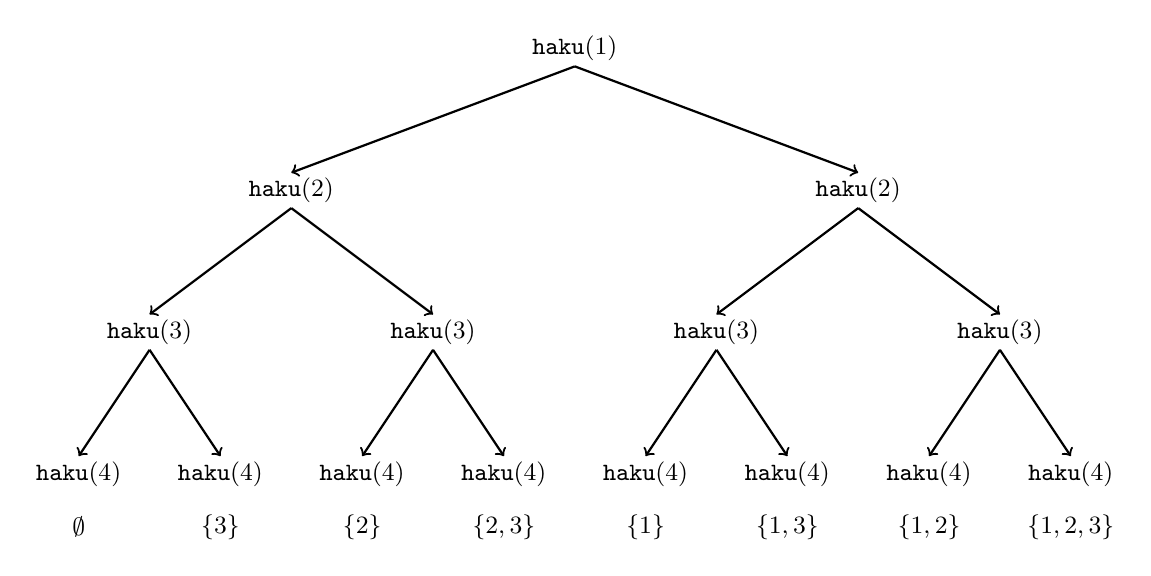
\begin{tikzpicture}[scale=.45]
  \begin{scope}
    \small
    \node at (0,0) {$\texttt{haku}(1)$};

    \node at (-8,-4) {$\texttt{haku}(2)$};
    \node at (8,-4) {$\texttt{haku}(2)$};

    \path[draw,thick,->] (0,0-0.5) -- (-8,-4+0.5);
    \path[draw,thick,->] (0,0-0.5) -- (8,-4+0.5);

    \node at (-12,-8) {$\texttt{haku}(3)$};
    \node at (-4,-8) {$\texttt{haku}(3)$};
    \node at (4,-8) {$\texttt{haku}(3)$};
    \node at (12,-8) {$\texttt{haku}(3)$};

    \path[draw,thick,->] (-8,-4-0.5) -- (-12,-8+0.5);
    \path[draw,thick,->] (-8,-4-0.5) -- (-4,-8+0.5);
    \path[draw,thick,->] (8,-4-0.5) -- (4,-8+0.5);
    \path[draw,thick,->] (8,-4-0.5) -- (12,-8+0.5);

    \node at (-14,-12) {$\texttt{haku}(4)$};
    \node at (-10,-12) {$\texttt{haku}(4)$};
    \node at (-6,-12) {$\texttt{haku}(4)$};
    \node at (-2,-12) {$\texttt{haku}(4)$};
    \node at (2,-12) {$\texttt{haku}(4)$};
    \node at (6,-12) {$\texttt{haku}(4)$};
    \node at (10,-12) {$\texttt{haku}(4)$};
    \node at (14,-12) {$\texttt{haku}(4)$};

    \node at (-14,-13.5) {$\emptyset$};
    \node at (-10,-13.5) {$\{3\}$};
    \node at (-6,-13.5) {$\{2\}$};
    \node at (-2,-13.5) {$\{2,3\}$};
    \node at (2,-13.5) {$\{1\}$};
    \node at (6,-13.5) {$\{1,3\}$};
    \node at (10,-13.5) {$\{1,2\}$};
    \node at (14,-13.5) {$\{1,2,3\}$};


    \path[draw,thick,->] (-12,-8-0.5) -- (-14,-12+0.5);
    \path[draw,thick,->] (-12,-8-0.5) -- (-10,-12+0.5);
    \path[draw,thick,->] (-4,-8-0.5) -- (-6,-12+0.5);
    \path[draw,thick,->] (-4,-8-0.5) -- (-2,-12+0.5);
    \path[draw,thick,->] (4,-8-0.5) -- (2,-12+0.5);
    \path[draw,thick,->] (4,-8-0.5) -- (6,-12+0.5);
    \path[draw,thick,->] (12,-8-0.5) -- (10,-12+0.5);
    \path[draw,thick,->] (12,-8-0.5) -- (14,-12+0.5);
\end{scope}
\end{tikzpicture}
\end{center}

\subsubsection{Menetelmä 2}

Toinen tapa käydä osajoukot läpi on hyödyntää kokonaislukujen
bittiesitystä. Jokainen $n$ alkion osajoukko
voidaan esittää $n$ bitin jonona,
joka taas vastaa lukua väliltä $0 \ldots 2^n-1$.
Bittiesityksen ykkösbitit ilmaisevat,
mitkä joukon alkiot on valittu osajoukkoon.

Tavallinen käytäntö on tulkita kokonaisluvun
bittiesitys osajoukkona niin,
että alkio $k$ kuuluu osajoukkoon,
jos lopusta lukien $k$. bitti on 1.
Esimerkiksi luvun 25 bittiesitys on 11001,
mikä vastaa osajoukkoa $\{1,4,5\}$.

Seuraava koodi käy läpi $n$ alkion joukon
osajoukkojen bittiesitykset:

\begin{lstlisting}
for (int b = 0; b < (1<<n); b++) {
    // käsittele osajoukko b
}
\end{lstlisting}

Seuraava koodi muodostaa jokaisen osajoukon
kohdalla vektorin \texttt{v},
joka sisältää osajoukossa olevat luvut.
Ne saadaan selville tutkimalla, mitkä bitit ovat
ykkösiä osajoukon bittiesityksessä.

\begin{lstlisting}
for (int b = 0; b < (1<<n); b++) {
    vector<int> v;
    for (int i = 0; i < n; i++) {
        if (b&(1<<i)) v.push_back(i+1);
    }
}
\end{lstlisting}

\section{Permutaatioiden läpikäynti}

\index{permutaatio@permutaatio}

Toinen usein esiintyvä tilanne on,
että tehtävän ratkaisut ovat $n$-alkioisen
joukon permutaatioita,
jolloin täydellisen haun tulee
käydä läpi $n!$ mahdollista permutaatiota.
Myös tässä tapauksessa on kaksi luontevaa
menetelmää täydellisen haun toteuttamiseen.

\subsubsection{Menetelmä 1}

Osajoukkojen tavoin permutaatioita voi muodostaa
rekursiivisesti.
Seuraava funktio \texttt{haku} käy läpi
joukon $\{1,2,\ldots,n\}$ permutaatiot.
Funktio muodostaa kunkin permutaation
vuorollaan vektoriin \texttt{v}.
Permutaatioiden muodostus alkaa kutsumalla
funktiota ilman parametreja.

\begin{lstlisting}
void haku() {
    if (v.size() == n) {
        // käsittele permutaatio v
    } else {
        for (int i = 1; i <= n; i++) {
            if (p[i]) continue;
            p[i] = 1;
            v.push_back(i);
            haku();
            p[i] = 0;
            v.pop_back();
        }
    }
}
\end{lstlisting}

Funktion jokainen kutsu lisää uuden
luvun permutaatioon vektoriin \texttt{v}.
Taulukko \texttt{p} kertoo, mitkä luvut on jo
valittu permutaatioon.
Jos $\texttt{p}[k]=0$, luku $k$ ei ole mukana,
ja jos $\texttt{p}[k]=1$, luku $k$ on mukana.
Jos vektorin \texttt{v} koko on sama kuin
joukon koko $n$, permutaatio on tullut valmiiksi.

\subsubsection{Menetelmä 2}

\index{next\_permutation@\texttt{next\_permutation}}

Toinen ratkaisu on aloittaa permutaatiosta
$\{1,2,\ldots,n\}$ ja muodostaa joka askeleella
järjestyksessä seuraava permutaatio.
C++:n standardikirjastossa on funktio
\texttt{next\_permutation}, joka tekee tämän muunnoksen.
Seuraava koodi käy läpi joukon $\{1,2,\ldots,n\}$
permutaatiot funktion avulla:

\begin{lstlisting}
vector<int> v;
for (int i = 1; i <= n; i++) {
    v.push_back(i);
}
do {
    // käsittele permutaatio v
} while (next_permutation(v.begin(),v.end()));
\end{lstlisting}

\section{Peruuttava haku}

\index{peruuttava haku@peruuttava haku}

\key{Peruuttava haku}
aloittaa ratkaisun etsimisen tyhjästä
ja laajentaa ratkaisua askel kerrallaan.
Joka askeleella haku haarautuu kaikkiin
mahdollisiin suuntiin, joihin ratkaisua voi laajentaa.
Haaran tutkimisen jälkeen haku peruuttaa takaisin
ja jatkaa muihin mahdollisiin suuntiin.

\index{kuningatarongelma}

Tarkastellaan esimerkkinä \key{kuningatarongelmaa},
jossa laskettavana on,
monellako tavalla $n \times n$ -shakkilaudalle
voidaan asettaa $n$ kuningatarta niin,
että mitkään kaksi kuningatarta eivät uhkaa toisiaan.
Esimerkiksi kun $n=4$, mahdolliset ratkaisut ovat seuraavat:

\begin{center}
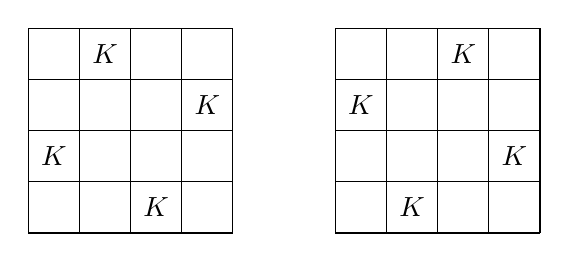
\begin{tikzpicture}[scale=.65]
  \begin{scope}
    \draw (0, 0) grid (4, 4);
    \node at (1.5,3.5) {$K$};
    \node at (3.5,2.5) {$K$};
    \node at (0.5,1.5) {$K$};
    \node at (2.5,0.5) {$K$};

    \draw (6, 0) grid (10, 4);
    \node at (6+2.5,3.5) {$K$};
    \node at (6+0.5,2.5) {$K$};
    \node at (6+3.5,1.5) {$K$};
    \node at (6+1.5,0.5) {$K$};

  \end{scope}
\end{tikzpicture}
\end{center}

Tehtävän voi ratkaista peruuttavalla haulla
muodostamalla ratkaisua rivi kerrallaan.
Jokaisella rivillä täytyy valita yksi ruuduista,
johon sijoitetaan kuningatar niin,
ettei se uhkaa mitään aiemmin lisättyä kuningatarta.
Ratkaisu on valmis, kun viimeisellekin
riville on lisätty kuningatar.

Esimerkiksi kun $n=4$, osa peruuttavan haun muodostamasta
puusta näyttää seuraavalta:

\begin{center}
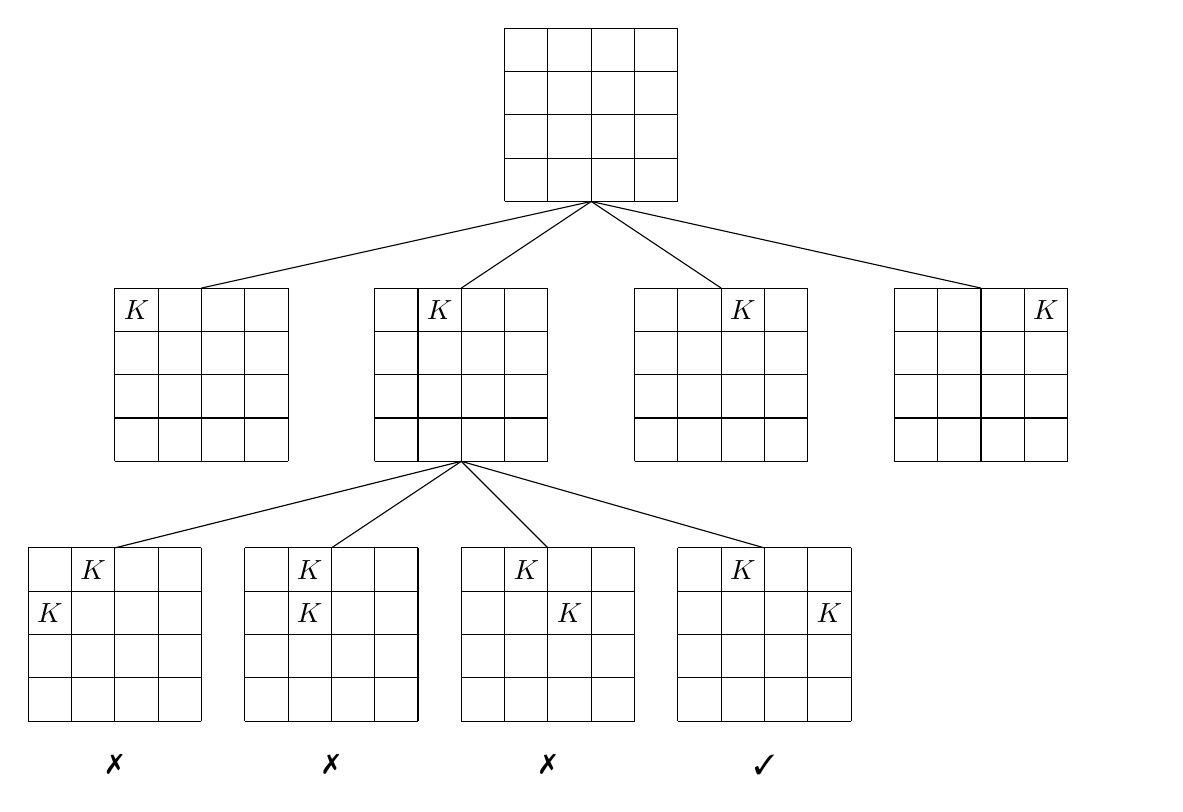
\begin{tikzpicture}[scale=.55]
  \begin{scope}
    \draw (0, 0) grid (4, 4);

    \draw (-9, -6) grid (-5, -2);
    \draw (-3, -6) grid (1, -2);
    \draw (3, -6) grid (7, -2);
    \draw (9, -6) grid (13, -2);

    \node at (-9+0.5,-3+0.5) {$K$};
    \node at (-3+1+0.5,-3+0.5) {$K$};
    \node at (3+2+0.5,-3+0.5) {$K$};
    \node at (9+3+0.5,-3+0.5) {$K$};

    \draw (2,0) -- (-7,-2);
    \draw (2,0) -- (-1,-2);
    \draw (2,0) -- (5,-2);
    \draw (2,0) -- (11,-2);

    \draw (-11, -12) grid (-7, -8);
    \draw (-6, -12) grid (-2, -8);
    \draw (-1, -12) grid (3, -8);
    \draw (4, -12) grid (8, -8);
    \draw[white] (11, -12) grid (15, -8);
    \node at (-11+1+0.5,-9+0.5) {$K$};
    \node at (-6+1+0.5,-9+0.5) {$K$};
    \node at (-1+1+0.5,-9+0.5) {$K$};
    \node at (4+1+0.5,-9+0.5) {$K$};
    \node at (-11+0+0.5,-10+0.5) {$K$};
    \node at (-6+1+0.5,-10+0.5) {$K$};
    \node at (-1+2+0.5,-10+0.5) {$K$};
    \node at (4+3+0.5,-10+0.5) {$K$};

    \draw (-1,-6) -- (-9,-8);
    \draw (-1,-6) -- (-4,-8);
    \draw (-1,-6) -- (1,-8);
    \draw (-1,-6) -- (6,-8);

    \node at (-9,-13) {\ding{55}};
    \node at (-4,-13) {\ding{55}};
    \node at (1,-13) {\ding{55}};
    \node at (6,-13) {\ding{51}};

  \end{scope}
\end{tikzpicture}
\end{center}

Kuvan alimmalla tasolla kolme ensimmäistä osaratkaisua
eivät kelpaa, koska niissä kuningattaret uhkaavat
toisiaan.
Sen sijaan neljäs osaratkaisu kelpaa,
ja sitä on mahdollista laajentaa loppuun asti
kokonaiseksi ratkaisuksi
asettamalla vielä kaksi kuningatarta laudalle.

\begin{samepage}
Seuraava koodi toteuttaa peruuttavan haun:

\begin{lstlisting}
void haku(int y) {
    if (y == n) {
        c++;
        return;
    }
    for (int x = 0; x < n; x++) {
        if (r1[x] || r2[x+y] || r3[x-y+n-1]) continue;
        r1[x] = r2[x+y] = r3[x-y+n-1] = 1;
        haku(y+1);
        r1[x] = r2[x+y] = r3[x-y+n-1] = 0;
    }
}
\end{lstlisting}
\end{samepage}
Haku alkaa kutsumalla funktiota \texttt{haku(0)}.
Laudan koko on muuttujassa $n$,
ja koodi laskee ratkaisuiden määrän
muuttujaan $c$.

Koodi olettaa, että laudan vaaka- ja pystyrivit
on numeroitu 0:sta alkaen.
Funktio asettaa kuningattaren vaakariville $y$,
kun $0 \le y < n$.
Jos taas $y=n$, yksi ratkaisu on valmis
ja funktio kasvattaa muuttujaa $c$.

Taulukko \texttt{r1} pitää kirjaa,
millä laudan pystyriveillä on jo kuningatar.
Vastaavasti taulukot \texttt{r2} ja \texttt{r3}
pitävät kirjaa vinoriveistä.
Tällaisille riveille ei voi laittaa enää toista
kuningatarta.
Esimerkiksi $4 \times 4$ -laudan tapauksessa
rivit on numeroitu seuraavasti:

\begin{center}
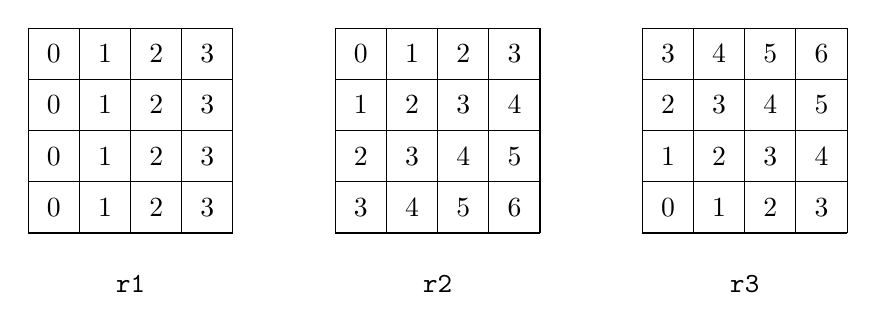
\begin{tikzpicture}[scale=.65]
  \begin{scope}
    \draw (0-6, 0) grid (4-6, 4);
    \node at (-6+0.5,3.5) {$0$};
    \node at (-6+1.5,3.5) {$1$};
    \node at (-6+2.5,3.5) {$2$};
    \node at (-6+3.5,3.5) {$3$};
    \node at (-6+0.5,2.5) {$0$};
    \node at (-6+1.5,2.5) {$1$};
    \node at (-6+2.5,2.5) {$2$};
    \node at (-6+3.5,2.5) {$3$};
    \node at (-6+0.5,1.5) {$0$};
    \node at (-6+1.5,1.5) {$1$};
    \node at (-6+2.5,1.5) {$2$};
    \node at (-6+3.5,1.5) {$3$};
    \node at (-6+0.5,0.5) {$0$};
    \node at (-6+1.5,0.5) {$1$};
    \node at (-6+2.5,0.5) {$2$};
    \node at (-6+3.5,0.5) {$3$};

    \draw (0, 0) grid (4, 4);
    \node at (0.5,3.5) {$0$};
    \node at (1.5,3.5) {$1$};
    \node at (2.5,3.5) {$2$};
    \node at (3.5,3.5) {$3$};
    \node at (0.5,2.5) {$1$};
    \node at (1.5,2.5) {$2$};
    \node at (2.5,2.5) {$3$};
    \node at (3.5,2.5) {$4$};
    \node at (0.5,1.5) {$2$};
    \node at (1.5,1.5) {$3$};
    \node at (2.5,1.5) {$4$};
    \node at (3.5,1.5) {$5$};
    \node at (0.5,0.5) {$3$};
    \node at (1.5,0.5) {$4$};
    \node at (2.5,0.5) {$5$};
    \node at (3.5,0.5) {$6$};

    \draw (6, 0) grid (10, 4);
    \node at (6.5,3.5) {$3$};
    \node at (7.5,3.5) {$4$};
    \node at (8.5,3.5) {$5$};
    \node at (9.5,3.5) {$6$};
    \node at (6.5,2.5) {$2$};
    \node at (7.5,2.5) {$3$};
    \node at (8.5,2.5) {$4$};
    \node at (9.5,2.5) {$5$};
    \node at (6.5,1.5) {$1$};
    \node at (7.5,1.5) {$2$};
    \node at (8.5,1.5) {$3$};
    \node at (9.5,1.5) {$4$};
    \node at (6.5,0.5) {$0$};
    \node at (7.5,0.5) {$1$};
    \node at (8.5,0.5) {$2$};
    \node at (9.5,0.5) {$3$};

    \node at (-4,-1) {\texttt{r1}};
    \node at (2,-1) {\texttt{r2}};
    \node at (8,-1) {\texttt{r3}};

  \end{scope}
\end{tikzpicture}
\end{center}

Koodin avulla selviää esimerkiksi,
että tapauksessa $n=8$ on 92 tapaa sijoittaa 8
kuningatarta $8 \times 8$ -laudalle.
Kun $n$ kasvaa, koodi hidastuu nopeasti,
koska ratkaisujen määrä kasvaa räjähdysmäisesti.
Tapauksen $n=16$ laskeminen vie jo noin minuutin
nykyaikaisella tietokoneella (14772512 ratkaisua).

\section{Haun optimointi}

Peruuttavaa hakua on usein mahdollista tehostaa
erilaisten optimointien avulla.
Tavoitteena on lisätä hakuun ''älykkyyttä''
niin, että haku pystyy havaitsemaan
mahdollisimman aikaisin,
jos muodosteilla oleva ratkaisu ei voi
johtaa kokonaiseen ratkaisuun.
Tällaiset optimoinnit karsivat haaroja
hakupuusta, millä voi olla suuri vaikutus
peruuttavan haun tehokkuuteen.

Tarkastellaan esimerkkinä tehtävää,
jossa laskettavana on reittien määrä
$n \times n$ -ruudukon
vasemmasta yläkulmasta oikeaan alakulmaan,
kun reitin aikana tulee käydä tarkalleen kerran 
jokaisessa ruudussa.
Esimerkiksi $7 \times 7$ -ruudukossa on
111712 mahdollista reittiä vasemmasta yläkulmasta
oikeaan alakulmaan, joista yksi on seuraava:

\begin{center}
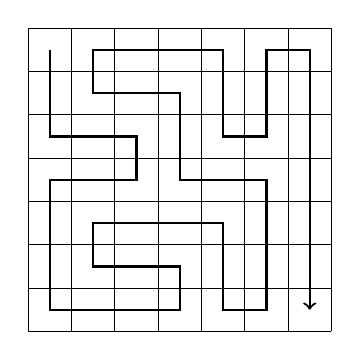
\begin{tikzpicture}[scale=.55]
  \begin{scope}
    \draw (0, 0) grid (7, 7);
    \draw[thick,->] (0.5,6.5) -- (0.5,4.5) -- (2.5,4.5) --
          (2.5,3.5) -- (0.5,3.5) -- (0.5,0.5) --
          (3.5,0.5) -- (3.5,1.5) -- (1.5,1.5) --
          (1.5,2.5) -- (4.5,2.5) -- (4.5,0.5) --
          (5.5,0.5) -- (5.5,3.5) -- (3.5,3.5) --
          (3.5,5.5) -- (1.5,5.5) -- (1.5,6.5) --
          (4.5,6.5) -- (4.5,4.5) -- (5.5,4.5) --
          (5.5,6.5) -- (6.5,6.5) -- (6.5,0.5);
  \end{scope}
\end{tikzpicture}
\end{center}

Keskitymme seuraavaksi nimenomaan tapaukseen $7 \times 7$,
koska se on laskennallisesti sopivan haastava.
Lähdemme liikkeelle suoraviivaisesta peruuttavaa hakua
käyttävästä algoritmista
ja teemme siihen pikkuhiljaa optimointeja,
jotka nopeuttavat hakua eri tavoin.
Mittaamme jokaisen optimoinnin jälkeen
algoritmin suoritusajan sekä rekursiokutsujen yhteismäärän,
jotta näemme selvästi, mikä vaikutus kullakin
optimoinnilla on haun tehokkuuteen.

\subsubsection{Perusalgoritmi}

Algoritmin ensimmäisessä versiossa ei ole mitään optimointeja,
vaan peruuttava haku käy läpi kaikki mahdolliset tavat
muodostaa reitti ruudukon vasemmasta yläkulmasta
oikeaan alakulmaan.

\begin{itemize}
\item
suoritusaika: 483 sekuntia
\item
rekursiokutsuja: 76 miljardia
\end{itemize}

\subsubsection{Optimointi 1}

Reitin ensimmäinen askel on joko alaspäin
tai oikealle. Tästä valinnasta seuraavat tilanteet
ovat symmetrisiä ruudukon lävistäjän suhteen.
Esimerkiksi seuraavat ratkaisut ovat
symmetrisiä keskenään:

\begin{center}
\begin{tabular}{ccc}
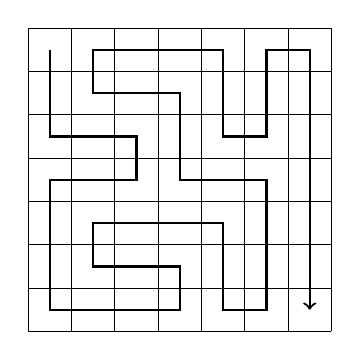
\begin{tikzpicture}[scale=.55]
  \begin{scope}
    \draw (0, 0) grid (7, 7);
    \draw[thick,->] (0.5,6.5) -- (0.5,4.5) -- (2.5,4.5) --
          (2.5,3.5) -- (0.5,3.5) -- (0.5,0.5) --
          (3.5,0.5) -- (3.5,1.5) -- (1.5,1.5) --
          (1.5,2.5) -- (4.5,2.5) -- (4.5,0.5) --
          (5.5,0.5) -- (5.5,3.5) -- (3.5,3.5) --
          (3.5,5.5) -- (1.5,5.5) -- (1.5,6.5) --
          (4.5,6.5) -- (4.5,4.5) -- (5.5,4.5) --
          (5.5,6.5) -- (6.5,6.5) -- (6.5,0.5);
  \end{scope}
\end{tikzpicture}
& \hspace{20px}
& 
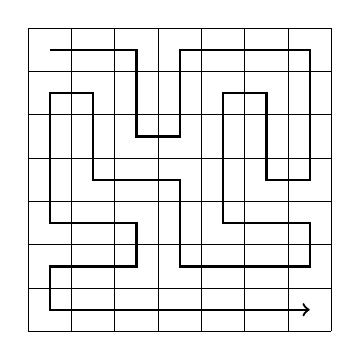
\begin{tikzpicture}[scale=.55]
  \begin{scope}[yscale=1,xscale=-1,rotate=-90]
    \draw (0, 0) grid (7, 7);
    \draw[thick,->] (0.5,6.5) -- (0.5,4.5) -- (2.5,4.5) --
          (2.5,3.5) -- (0.5,3.5) -- (0.5,0.5) --
          (3.5,0.5) -- (3.5,1.5) -- (1.5,1.5) --
          (1.5,2.5) -- (4.5,2.5) -- (4.5,0.5) --
          (5.5,0.5) -- (5.5,3.5) -- (3.5,3.5) --
          (3.5,5.5) -- (1.5,5.5) -- (1.5,6.5) --
          (4.5,6.5) -- (4.5,4.5) -- (5.5,4.5) --
          (5.5,6.5) -- (6.5,6.5) -- (6.5,0.5);
  \end{scope}
\end{tikzpicture}
\end{tabular}
\end{center}

Tämän ansiosta voimme tehdä päätöksen,
että reitin ensimmäinen askel on alaspäin,
ja kertoa lopuksi reittien määrän 2:lla.

\begin{itemize}
\item
suoritusaika: 244 sekuntia
\item
rekursiokutsuja: 38 miljardia
\end{itemize}

\subsubsection{Optimointi 2}

Jos reitti menee oikean alakulman ruutuun ennen kuin
se on käynyt kaikissa muissa ruuduissa,
siitä ei voi mitenkään enää saada kelvollista ratkaisua.
Näin on esimerkiksi seuraavassa tilanteessa:

\begin{center}
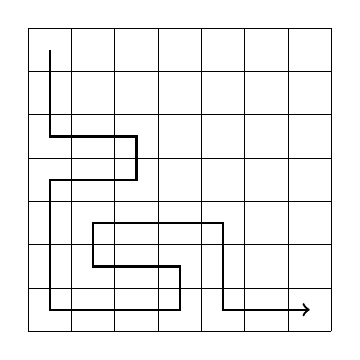
\begin{tikzpicture}[scale=.55]
  \begin{scope}
    \draw (0, 0) grid (7, 7);
    \draw[thick,->] (0.5,6.5) -- (0.5,4.5) -- (2.5,4.5) --
          (2.5,3.5) -- (0.5,3.5) -- (0.5,0.5) --
          (3.5,0.5) -- (3.5,1.5) -- (1.5,1.5) --
          (1.5,2.5) -- (4.5,2.5) -- (4.5,0.5) --
          (6.5,0.5);
  \end{scope}
\end{tikzpicture}
\end{center}
Niinpä voimme keskeyttää hakuhaaran heti,
jos tulemme oikean alakulman ruutuun liian aikaisin.
\begin{itemize}
\item
suoritusaika: 119 sekuntia
\item
rekursiokutsuja: 20 miljardia
\end{itemize}

\subsubsection{Optimointi 3}

Jos reitti osuu seinään niin, että kummallakin puolella
on ruutu, jossa reitti ei ole vielä käynyt,
ruudukko jakautuu kahteen osaan.
Esimerkiksi seuraavassa tilanteessa
sekä vasemmalla että
oikealla puolella on tyhjä ruutu:

\begin{center}
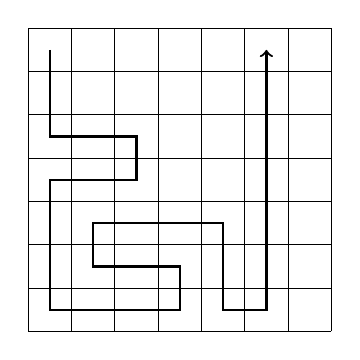
\begin{tikzpicture}[scale=.55]
  \begin{scope}
    \draw (0, 0) grid (7, 7);
    \draw[thick,->] (0.5,6.5) -- (0.5,4.5) -- (2.5,4.5) --
          (2.5,3.5) -- (0.5,3.5) -- (0.5,0.5) --
          (3.5,0.5) -- (3.5,1.5) -- (1.5,1.5) --
          (1.5,2.5) -- (4.5,2.5) -- (4.5,0.5) --
          (5.5,0.5) -- (5.5,6.5);
  \end{scope}
\end{tikzpicture}
\end{center}
Nyt ei ole enää mahdollista käydä kaikissa ruuduissa,
joten voimme keskeyttää hakuhaaran.
Tämä optimointi on hyvin hyödyllinen:

\begin{itemize}
\item
suoritusaika: 1{,}8 sekuntia
\item
rekursiokutsuja: 221 miljoonaa
\end{itemize}

\subsubsection{Optimointi 4}

Äskeisen optimoinnin ideaa voi yleistää:
ruudukko jakaantuu kahteen osaan,
jos nykyisen ruudun ylä- ja alapuolella on
tyhjä ruutu sekä vasemmalla ja oikealla
puolella on seinä tai aiemmin käyty ruutu
(tai päinvastoin).

Esimerkiksi seuraavassa tilanteessa
nykyisen ruudun ylä- ja alapuolella on
tyhjä ruutu eikä reitti voi enää edetä
molempiin ruutuihin:
\begin{center}
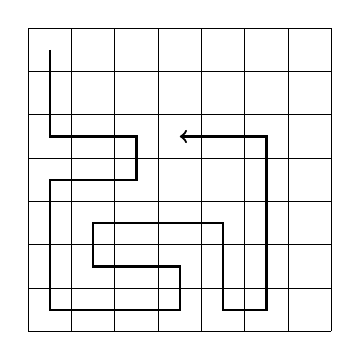
\begin{tikzpicture}[scale=.55]
  \begin{scope}
    \draw (0, 0) grid (7, 7);
    \draw[thick,->] (0.5,6.5) -- (0.5,4.5) -- (2.5,4.5) --
          (2.5,3.5) -- (0.5,3.5) -- (0.5,0.5) --
          (3.5,0.5) -- (3.5,1.5) -- (1.5,1.5) --
          (1.5,2.5) -- (4.5,2.5) -- (4.5,0.5) --
          (5.5,0.5) -- (5.5,4.5) -- (3.5,4.5);
  \end{scope}
\end{tikzpicture}
\end{center}
Haku tehostuu entisestään, kun keskeytämme
hakuhaaran kaikissa tällaisissa tapauksissa:

\begin{itemize}
\item
suoritusaika: 0{,}6 sekuntia
\item
rekursiokutsuja: 69 miljoonaa
\end{itemize}

~\\
Nyt on hyvä hetki lopettaa optimointi ja muistella,
mistä lähdimme liikkeelle.
Alkuperäinen algoritmi vei aikaa 483 sekuntia,
ja nyt optimointien jälkeen algoritmi vie aikaa
vain 0{,}6 sekuntia.
Optimointien ansiosta algoritmi nopeutui
siis lähes 1000-kertaisesti.

Tämä on yleinen ilmiö peruuttavassa haussa,
koska hakupuu on yleensä valtava ja
yksinkertainenkin optimointi voi karsia suuren
määrän haaroja hakupuusta.
Erityisen hyödyllisiä ovat optimoinnit,
jotka kohdistuvat hakupuun yläosaan,
koska ne karsivat eniten haaroja.

\section{Puolivälihaku}

\index{puolivxlihaku@puolivälihaku}

\key{Puolivälihaku} (''meet in the middle'') on tekniikka,
jossa hakutehtävä jaetaan kahteen yhtä suureen osaan.
Kumpaankin osaan tehdään erillinen haku,
ja lopuksi hakujen tulokset yhdistetään.

Puolivälihaun käyttäminen edellyttää,
että erillisten hakujen tulokset pystyy
yhdistämään tehokkaasti.
Tällöin puolivälihaku on tehokkaampi
kuin yksi haku, joka käy läpi koko hakualueen.
Tyypillisesti puolivälihaku tehostaa algoritmia
niin, että aikavaativuuden kertoimesta $2^n$
tulee kerroin $2^{n/2}$.

Tarkastellaan ongelmaa, jossa annettuna
on $n$ lukua sisältävä lista sekä kokonaisluku $x$.
Tehtävänä on selvittää, voiko listalta valita
joukon lukuja niin, että niiden summa on $x$.
Esimerkiksi jos lista on $[2,4,5,9]$ ja $x=15$,
voimme valita listalta luvut $[2,4,9]$,
jolloin $2+4+9=15$.
Jos taas lista säilyy ennallaan ja $x=10$,
mikään valinta ei täytä vaatimusta.

Tavanomainen ratkaisu tehtävään on käydä kaikki
listan alkioiden osajoukot läpi ja tarkastaa,
onko jonkin osajoukon summa $x$.
Tällainen ratkaisu kuluttaa aikaa $O(2^n)$,
koska erilaisia osajoukkoja on $2^n$.
Seuraavaksi näemme,
miten puolivälihaun avulla on mahdollista luoda
tehokkaampi $O(2^{n/2})$-aikainen ratkaisu.
Huomaa, että aikavaativuuksissa $O(2^n)$ ja
$O(2^{n/2})$ on merkittävä ero, koska
$2^{n/2}$ tarkoittaa samaa kuin $\sqrt{2^n}$.

Ideana on jakaa syötteenä oleva lista
kahteen listaan $A$ ja $B$,
joista kumpikin sisältää noin puolet luvuista.
Ensimmäinen haku muodostaa kaikki osajoukot
listan $A$ luvuista ja laittaa muistiin niiden summat
listaan $S_A$.
Toinen haku muodostaa vastaavasti listan
$B$ perusteella listan $S_B$.
Tämän jälkeen riittää tarkastaa,
onko mahdollista valita yksi luku listasta $S_A$
ja toinen luku listasta $S_B$ niin,
että lukujen summa on $x$.
Tämä on mahdollista tarkalleen silloin,
kun alkuperäisen listan luvuista saa summan $x$.

Tarkastellaan esimerkkiä,
jossa lista on $[2,4,5,9]$
ja $x=15$.
Puolivälihaku jakaa luvut kahteen
listaan niin, että $A=[2,4]$
ja $B=[5,9]$.
Näistä saadaan edelleen summalistat
$S_A=[0,2,4,6]$ ja $S_B=[0,5,9,14]$.
Summa $x=15$ on mahdollista muodostaa,
koska voidaan valita $S_A$:sta luku $6$
ja $S_B$:stä luku $9$.
Tämä valinta vastaa ratkaisua $[2,4,9]$.

Ratkaisun aikavaativuus on $O(2^{n/2})$,
koska kummassakin listassa $A$ ja $B$
on $n/2$ lukua ja niiden osajoukkojen
summien laskeminen listoihin $S_A$ ja $S_B$
vie aikaa $O(2^{n/2})$.
Tämän jälkeen on mahdollista tarkastaa
ajassa $O(2^{n/2})$, voiko summaa $x$ muodostaa
listojen $S_A$ ja $S_B$ luvuista.
\chapter{Greedy algorithms}

\index{greedy algorithm}

A \key{greedy algorithm}
constructs a solution to the problem
by always making a choice that looks
the best at the moment.
A greedy algorithm never takes back
its choices, but directly constructs
the final solution.
For this reason, greedy algorithms
are usually very efficient.

The difficulty in designing greedy algorithms
is to find a greedy strategy
that always produces an optimal solution
to the problem.
The locally optimal choices in a greedy
algorithm should also be globally optimal.
It is often difficult to argue that
a greedy algorithm works.

\section{Coin problem}

As a first example, we consider a problem
where we are given a set of coin values
and our task is to form a sum of money
using the coins.
The values of the coins are
$\{c_1,c_2,\ldots,c_k\}$,
and each coin can be used as many times we want.
What is the minimum number of coins needed?

For example, if the coins are the euro coins (in cents)
\[\{1,2,5,10,20,50,100,200\}\]
and the sum of money is 520,
we need at least four coins.
The optimal solution is to select coins
$200+200+100+20$ whose sum is 520.

\subsubsection{Greedy algorithm}

A simple greedy algorithm to the problem
is to always select the largest possible coin,
until we have constructed the required sum of money.
This algorithm works in the example case,
because we first select two 200 cent coins,
then one 100 cent coin and finally one 20 cent coin.
But does this algorithm always work?

It turns out that, for the set of euro coins,
the greedy algorithm \emph{always} works, i.e.,
it always produces a solution with the fewest
possible number of coins.
The correctness of the algorithm can be
shown as follows:

Each coin 1, 5, 10, 50 and 100 appears
at most once in an optimal solution.
The reason for this is that if the
solution would contain two such coins,
we could replace them by one coin and
obtain a better solution.
For example, if the solution would contain
coins $5+5$, we could replace them by coin $10$.

In the same way, coins 2 and 20 appear
at most twice in an optimal solution,
because we could replace
coins $2+2+2$ by coins $5+1$ and
coins $20+20+20$ by coins $50+10$.
Moreover, an optimal solution cannot contain
coins $2+2+1$ or $20+20+10$,
because we could replace them by coins $5$ and $50$.

Using these observations,
we can show for each coin $x$ that
it is not possible to optimally construct
a sum $x$ or any larger sum by only using coins
that are smaller than $x$.
For example, if $x=100$, the largest optimal
sum using the smaller coins is  $50+20+20+5+2+2=99$.
Thus, the greedy algorithm that always selects
the largest coin produces the optimal solution.

This example shows that it can be difficult
to argue that a greedy algorithm works,
even if the algorithm itself is simple.

\subsubsection{General case}

In the general case, the coin set can contain any coins
and the greedy algorithm \emph{does not} necessarily produce
an optimal solution.

We can prove that a greedy algorithm does not work
by showing a counterexample
where the algorithm gives a wrong answer.
In this problem we can easily find a counterexample:
if the coins are $\{1,3,4\}$ and the target sum
is 6, the greedy algorithm produces the solution
$4+1+1$ while the optimal solution is $3+3$.

We do not know if the general coin problem
can be solved using any greedy algorithm.
However, as we will see in Chapter 7,
the general problem can be efficiently
solved using a dynamic
programming algorithm that always gives the
correct answer.

\section{Scheduling}

Many scheduling problems can be solved
using greedy algorithms.
A classic problem is as follows:
Given $n$ events with their starting and ending
times, our goal is to plan a schedule
that includes as many events as possible.
It is not possible to select an event partially.
For example, consider the following events:
\begin{center}
\begin{tabular}{lll}
event & starting time & ending time \\
\hline
$A$ & 1 & 3 \\
$B$ & 2 & 5 \\
$C$ & 3 & 9 \\
$D$ & 6 & 8 \\
\end{tabular}
\end{center}
In this case the maximum number of events is two.
For example, we can select events $B$ and $D$
as follows:
\begin{center}
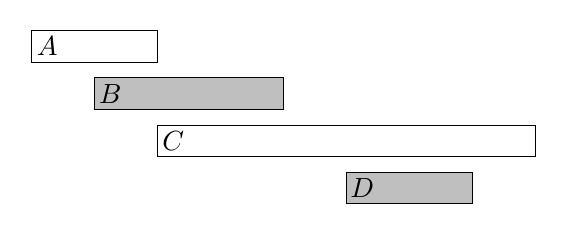
\begin{tikzpicture}[scale=.4]
  \begin{scope}
    \draw (2, 0) rectangle (6, -1);
    \draw[fill=lightgray] (4, -1.5) rectangle (10, -2.5);
    \draw (6, -3) rectangle (18, -4);
    \draw[fill=lightgray] (12, -4.5) rectangle (16, -5.5);
    \node at (2.5,-0.5) {$A$};
    \node at (4.5,-2) {$B$};
    \node at (6.5,-3.5) {$C$};
    \node at (12.5,-5) {$D$};
  \end{scope}
\end{tikzpicture}
\end{center}

It is possible to invent several greedy algorithms
for the problem, but which of them works in every case?

\subsubsection*{Algorithm 1}

The first idea is to select as \emph{short}
events as possible.
In the example case this algorithm
selects the following events:
\begin{center}
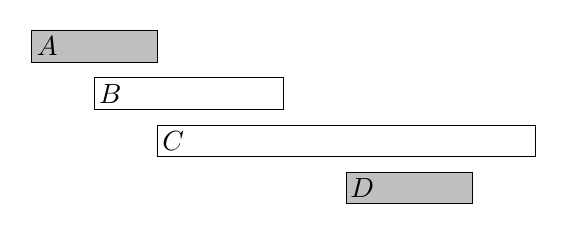
\begin{tikzpicture}[scale=.4]
  \begin{scope}
    \draw[fill=lightgray] (2, 0) rectangle (6, -1);
    \draw (4, -1.5) rectangle (10, -2.5);
    \draw (6, -3) rectangle (18, -4);
    \draw[fill=lightgray] (12, -4.5) rectangle (16, -5.5);
    \node at (2.5,-0.5) {$A$};
    \node at (4.5,-2) {$B$};
    \node at (6.5,-3.5) {$C$};
    \node at (12.5,-5) {$D$};
  \end{scope}
\end{tikzpicture}
\end{center}

However, selecting short events is not always
a correct strategy, but the algorithm fails,
for example, in the following case:
\begin{center}
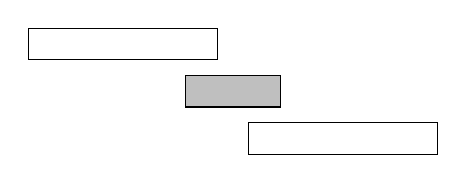
\begin{tikzpicture}[scale=.4]
  \begin{scope}
    \draw (1, 0) rectangle (7, -1);
    \draw[fill=lightgray] (6, -1.5) rectangle (9, -2.5);
    \draw (8, -3) rectangle (14, -4);
  \end{scope}
\end{tikzpicture}
\end{center}
If we select the short event, we can only select one event.
However, it would be possible to select both the long events.

\subsubsection*{Algorithm 2}

Another idea is to always select the next possible
event that \emph{begins} as \emph{early} as possible.
This algorithm selects the following events:
\begin{center}
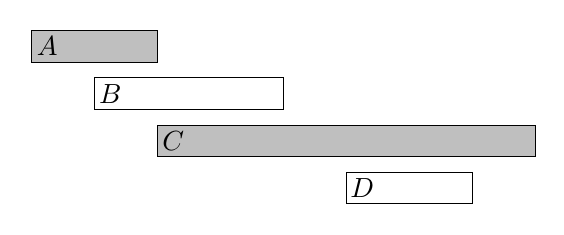
\begin{tikzpicture}[scale=.4]
  \begin{scope}
    \draw[fill=lightgray] (2, 0) rectangle (6, -1);
    \draw (4, -1.5) rectangle (10, -2.5);
    \draw[fill=lightgray] (6, -3) rectangle (18, -4);
    \draw (12, -4.5) rectangle (16, -5.5);
    \node at (2.5,-0.5) {$A$};
    \node at (4.5,-2) {$B$};
    \node at (6.5,-3.5) {$C$};
    \node at (12.5,-5) {$D$};
  \end{scope}
\end{tikzpicture}
\end{center}

However, we can find a counterexample
also for this algorithm.
For example, in the following case,
the algorithm only selects one event:
\begin{center}
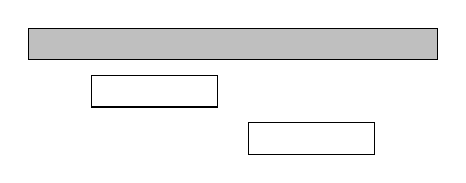
\begin{tikzpicture}[scale=.4]
  \begin{scope}
    \draw[fill=lightgray] (1, 0) rectangle (14, -1);
    \draw (3, -1.5) rectangle (7, -2.5);
    \draw (8, -3) rectangle (12, -4);
  \end{scope}
\end{tikzpicture}
\end{center}
If we select the first event, it is not possible
to select any other events.
However, it would be possible to select the
other two events.

\subsubsection*{Algorithm 3}

The third idea is to always select the next
possible event that \emph{ends} as \emph{early} as possible.
This algorithm selects the following events: 
\begin{center}
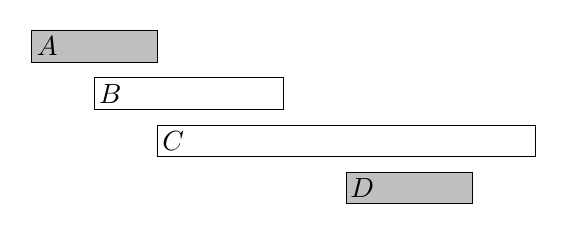
\begin{tikzpicture}[scale=.4]
  \begin{scope}
    \draw[fill=lightgray] (2, 0) rectangle (6, -1);
    \draw (4, -1.5) rectangle (10, -2.5);
    \draw (6, -3) rectangle (18, -4);
    \draw[fill=lightgray] (12, -4.5) rectangle (16, -5.5);
    \node at (2.5,-0.5) {$A$};
    \node at (4.5,-2) {$B$};
    \node at (6.5,-3.5) {$C$};
    \node at (12.5,-5) {$D$};
  \end{scope}
\end{tikzpicture}
\end{center}

It turns out that this algorithm
\emph{always} produces an optimal solution.
First, it is always an optimal choice
to first select an event that ends
as early as possible.
After this, it is an optimal choice
to select the next event
using the same strategy, etc.,
until we cannot select any more events.

One way to argue that the algorithm works
is to consider
what happens if we first select an event
that ends later than the event that ends
as early as possible.
Now, we will have at most an equal number of
choices how we can select the next event.
Hence, selecting an event that ends later
can never yield a better solution,
and the greedy algorithm is correct.

\section{Tasks and deadlines}

Let us now consider a problem where
we are given $n$ tasks with durations and deadlines
and our task is to choose an order to perform the tasks.
For each task, we earn $d-x$ points
where $d$ is the task's deadline
and $x$ is the moment when we finished the task.
What is the largest possible total score
we can obtain?

For example, suppose that the tasks are as follows:
\begin{center}
\begin{tabular}{lll}
task & duration & deadline \\
\hline
$A$ & 4 & 2 \\
$B$ & 3 & 5 \\
$C$ & 2 & 7 \\
$D$ & 4 & 5 \\
\end{tabular}
\end{center}
In this case, an optimal schedule for the tasks
is as follows:
\begin{center}
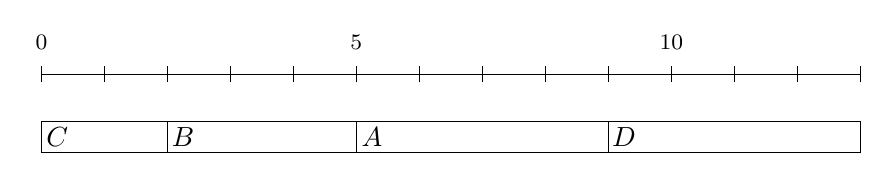
\begin{tikzpicture}[scale=.4]
  \begin{scope}
    \draw (0, 0) rectangle (4, -1);
    \draw (4, 0) rectangle (10, -1);
    \draw (10, 0) rectangle (18, -1);
    \draw (18, 0) rectangle (26, -1);
    \node at (0.5,-0.5) {$C$};
    \node at (4.5,-0.5) {$B$};
    \node at (10.5,-0.5) {$A$};
    \node at (18.5,-0.5) {$D$};

    \draw (0,1.5) -- (26,1.5);
    \foreach \i in {0,2,...,26}
    {
        \draw (\i,1.25) -- (\i,1.75);
    }
    \footnotesize
    \node at (0,2.5) {0};
    \node at (10,2.5) {5};
    \node at (20,2.5) {10};

  \end{scope}
\end{tikzpicture}
\end{center}
In this solution, $C$ yields 5 points,
$B$ yields 0 points, $A$ yields $-7$ points
and $D$ yields $-8$ points,
so the total score is $-10$.

Surprisingly, the optimal solution to the problem
does not depend on the deadlines at all,
but a correct greedy strategy is to simply
perform the tasks \emph{sorted by their durations}
in increasing order.
The reason for this is that if we ever perform
two tasks one after another such that the first task
takes longer than the second task,
we can obtain a better solution if we swap the tasks.
For example, consider the following schedule:
\begin{center}
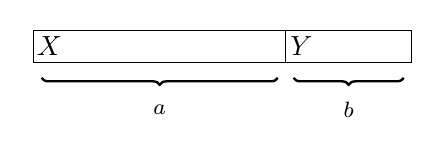
\begin{tikzpicture}[scale=.4]
  \begin{scope}
    \draw (0, 0) rectangle (8, -1);
    \draw (8, 0) rectangle (12, -1);
    \node at (0.5,-0.5) {$X$};
    \node at (8.5,-0.5) {$Y$};

\draw [decoration={brace}, decorate, line width=0.3mm] (7.75,-1.5) -- (0.25,-1.5);
\draw [decoration={brace}, decorate, line width=0.3mm] (11.75,-1.5) -- (8.25,-1.5);

\footnotesize
\node at (4,-2.5) {$a$};
\node at (10,-2.5) {$b$};

  \end{scope}
\end{tikzpicture}
\end{center}
Here $a>b$, so we should swap the tasks:
\begin{center}
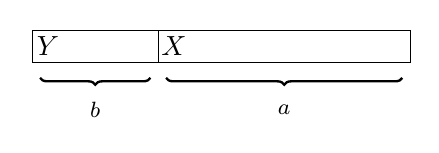
\begin{tikzpicture}[scale=.4]
  \begin{scope}
    \draw (0, 0) rectangle (4, -1);
    \draw (4, 0) rectangle (12, -1);
    \node at (0.5,-0.5) {$Y$};
    \node at (4.5,-0.5) {$X$};

\draw [decoration={brace}, decorate, line width=0.3mm] (3.75,-1.5) -- (0.25,-1.5);
\draw [decoration={brace}, decorate, line width=0.3mm] (11.75,-1.5) -- (4.25,-1.5);

\footnotesize
\node at (2,-2.5) {$b$};
\node at (8,-2.5) {$a$};

  \end{scope}
\end{tikzpicture}
\end{center}
Now $X$ gives $b$ points fewer and $Y$ gives $a$ points more,
so the total score increases by $a-b > 0$.
In an optimal solution,
for any two consecutive tasks,
it must hold that the shorter task comes
before the longer task.
Thus, the tasks must be performed
sorted by their durations.

\section{Minimizing sums}

We will next consider a problem where
we are given $n$ numbers $a_1,a_2,\ldots,a_n$
and our task is to find a value $x$
that minimizes the sum
\[|a_1-x|^c+|a_2-x|^c+\cdots+|a_n-x|^c.\]
We will focus on the cases $c=1$ and $c=2$.

\subsubsection{Case $c=1$}

In this case, we should minimize the sum
\[|a_1-x|+|a_2-x|+\cdots+|a_n-x|.\]
For example, if the numbers are $[1,2,9,2,6]$,
the best solution is to select $x=2$
which produces the sum
\[
|1-2|+|2-2|+|9-2|+|2-2|+|6-2|=12.
\]
In the general case, the best choice for $x$
is the \textit{median} of the numbers,
i.e., the middle number after sorting.
For example, the list $[1,2,9,2,6]$
becomes $[1,2,2,6,9]$ after sorting,
so the median is 2.

The median is an optimal choice,
because if $x$ is smaller than the median,
the sum becomes smaller by increasing $x$,
and if $x$ is larger then the median,
the sum becomes smaller by decreasing $x$.
Hence, the optimal solution is that $x$
is the median.
If $n$ is even and there are two medians,
both medians and all values between them
are optimal solutions.

\subsubsection{Case $c=2$}

In this case, we should minimize the sum
\[(a_1-x)^2+(a_2-x)^2+\cdots+(a_n-x)^2.\]
For example, if the numbers are $[1,2,9,2,6]$,
the best solution is to select $x=4$
which produces the sum
\[
(1-4)^2+(2-4)^2+(9-4)^2+(2-4)^2+(6-4)^2=46.
\]
In the general case, the best choice for $x$
is the \emph{average} of the numbers.
In the example the average is $(1+2+9+2+6)/5=4$.
This result can be derived by presenting
the sum as follows:
\[
nx^2 - 2x(a_1+a_2+\cdots+a_n) + (a_1^2+a_2^2+\cdots+a_n^2)
\]
The last part does not depend on $x$,
so we can ignore it.
The remaining parts form a function
$nx^2-2xs$ where $s=a_1+a_2+\cdots+a_n$.
This is a parabola opening upwards
with roots $x=0$ and $x=2s/n$,
and the minimum value is the average
of the roots $x=s/n$, i.e.,
the average of the numbers $a_1,a_2,\ldots,a_n$.

\section{Data compression}

\index{data compression}
\index{binary code}
\index{codeword}

A \key{binary code} assigns for each character
of a given string a \key{codeword} that consists of bits.
We can \emph{compress} the string using the binary code
by replacing each character by the
corresponding codeword.
For example, the following binary code
assigns codewords for characters
\texttt{A}–\texttt{D}:
\begin{center}
\begin{tabular}{rr}
character & codeword \\
\hline
\texttt{A} & 00 \\
\texttt{B} & 01 \\
\texttt{C} & 10 \\
\texttt{D} & 11 \\
\end{tabular}
\end{center}
This is a \key{constant-length} code
which means that the length of each
codeword is the same.
For example, we can compress the string
\texttt{AABACDACA} as follows:
\[00\,00\,01\,00\,10\,11\,00\,10\,00\]
Using this code, the length of the compressed
string is 18 bits.
However, we can compress the string better
if we use a \key{variable-length} code
where codewords may have different lengths.
Then we can give short codewords for
characters that appear often
and long codewords for characters
that appear rarely.
It turns out that an \key{optimal} code
for the above string is as follows:
\begin{center}
\begin{tabular}{rr}
character & codeword \\
\hline
\texttt{A} & 0 \\
\texttt{B} & 110 \\
\texttt{C} & 10 \\
\texttt{D} & 111 \\
\end{tabular}
\end{center}
An optimal code produces a compressed string
that is as short as possible.
In this case, the compressed string using
the optimal code is
\[0\,0\,110\,0\,10\,111\,0\,10\,0,\]
so only 15 bits are needed instead of 18 bits.
Thus, thanks to a better code it was possible to
save 3 bits in the compressed string.

We require that no codeword
is a prefix of another codeword.
For example, it is not allowed that a code
would contain both codewords 10
and 1011.
The reason for this is that we want
to be able to generate the original string
from the compressed string.
If a codeword could be a prefix of another codeword,
this would not always be possible.
For example, the following code is \emph{not} valid:
\begin{center}
\begin{tabular}{rr}
character & codeword \\
\hline
\texttt{A} & 10 \\
\texttt{B} & 11 \\
\texttt{C} & 1011 \\
\texttt{D} & 111 \\
\end{tabular}
\end{center}
Using this code, it would not be possible to know
if the compressed string 1011 corresponds to
the string \texttt{AB} or the string \texttt{C}.

\index{Huffman coding}

\subsubsection{Huffman coding}

\key{Huffman coding} is a greedy algorithm
that constructs an optimal code for
compressing a given string.
The algorithm builds a binary tree
based on the frequencies of the characters
in the string,
and each character's codeword can be read
by following a path from the root to
the corresponding node.
A move to the left corresponds to bit 0,
and a move to the right corresponds to bit 1.

Initially, each character of the string is
represented by a node whose weight is the
number of times the character occurs in the string.
Then at each step two nodes with minimum weights
are combined by creating
a new node whose weight is the sum of the weights
of the original nodes.
The process continues until all nodes have been combined.

Next we will see how Huffman coding creates
the optimal code for the string
\texttt{AABACDACA}.
Initially, there are four nodes that correspond
to the characters in the string:

\begin{center}
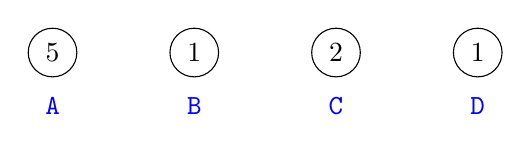
\begin{tikzpicture}[scale=0.9]
\node[draw, circle] (1) at (0,0) {$5$};
\node[draw, circle] (2) at (2,0) {$1$};
\node[draw, circle] (3) at (4,0) {$2$};
\node[draw, circle] (4) at (6,0) {$1$};

\node[color=blue] at (0,-0.75) {\texttt{A}};
\node[color=blue] at (2,-0.75) {\texttt{B}};
\node[color=blue] at (4,-0.75) {\texttt{C}};
\node[color=blue] at (6,-0.75) {\texttt{D}};

%\path[draw,thick,-] (4) -- (5);
\end{tikzpicture}
\end{center}
The node that represents character \texttt{A}
has weight 5 because character \texttt{A}
appears 5 times in the string.
The other weights have been calculated
in the same way.

The first step is to combine the nodes that
correspond to characters \texttt{B} and \texttt{D},
both with weight 1.
The result is:
\begin{center}
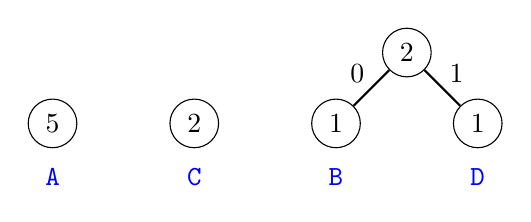
\begin{tikzpicture}[scale=0.9]
\node[draw, circle] (1) at (0,0) {$5$};
\node[draw, circle] (3) at (2,0) {$2$};
\node[draw, circle] (2) at (4,0) {$1$};
\node[draw, circle] (4) at (6,0) {$1$};
\node[draw, circle] (5) at (5,1) {$2$};

\node[color=blue] at (0,-0.75) {\texttt{A}};
\node[color=blue] at (2,-0.75) {\texttt{C}};
\node[color=blue] at (4,-0.75) {\texttt{B}};
\node[color=blue] at (6,-0.75) {\texttt{D}};

\node at (4.3,0.7) {0};
\node at (5.7,0.7) {1};

\path[draw,thick,-] (2) -- (5);
\path[draw,thick,-] (4) -- (5);
\end{tikzpicture}
\end{center}
After this, the nodes with weight 2 are combined:
\begin{center}
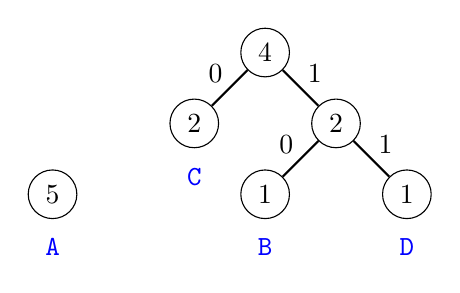
\begin{tikzpicture}[scale=0.9]
\node[draw, circle] (1) at (1,0) {$5$};
\node[draw, circle] (3) at (3,1) {$2$};
\node[draw, circle] (2) at (4,0) {$1$};
\node[draw, circle] (4) at (6,0) {$1$};
\node[draw, circle] (5) at (5,1) {$2$};
\node[draw, circle] (6) at (4,2) {$4$};

\node[color=blue] at (1,-0.75) {\texttt{A}};
\node[color=blue] at (3,1-0.75) {\texttt{C}};
\node[color=blue] at (4,-0.75) {\texttt{B}};
\node[color=blue] at (6,-0.75) {\texttt{D}};

\node at (4.3,0.7) {0};
\node at (5.7,0.7) {1};
\node at (3.3,1.7) {0};
\node at (4.7,1.7) {1};

\path[draw,thick,-] (2) -- (5);
\path[draw,thick,-] (4) -- (5);
\path[draw,thick,-] (3) -- (6);
\path[draw,thick,-] (5) -- (6);
\end{tikzpicture}
\end{center}
Finally, the two remaining nodes are combined:
\begin{center}
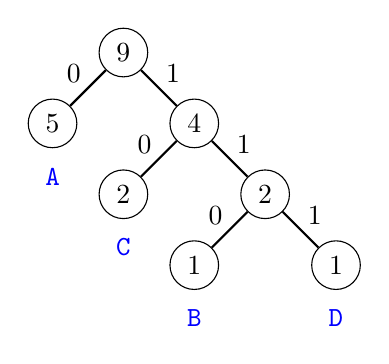
\begin{tikzpicture}[scale=0.9]
\node[draw, circle] (1) at (2,2) {$5$};
\node[draw, circle] (3) at (3,1) {$2$};
\node[draw, circle] (2) at (4,0) {$1$};
\node[draw, circle] (4) at (6,0) {$1$};
\node[draw, circle] (5) at (5,1) {$2$};
\node[draw, circle] (6) at (4,2) {$4$};
\node[draw, circle] (7) at (3,3) {$9$};

\node[color=blue] at (2,2-0.75) {\texttt{A}};
\node[color=blue] at (3,1-0.75) {\texttt{C}};
\node[color=blue] at (4,-0.75) {\texttt{B}};
\node[color=blue] at (6,-0.75) {\texttt{D}};

\node at (4.3,0.7) {0};
\node at (5.7,0.7) {1};
\node at (3.3,1.7) {0};
\node at (4.7,1.7) {1};
\node at (2.3,2.7) {0};
\node at (3.7,2.7) {1};

\path[draw,thick,-] (2) -- (5);
\path[draw,thick,-] (4) -- (5);
\path[draw,thick,-] (3) -- (6);
\path[draw,thick,-] (5) -- (6);
\path[draw,thick,-] (1) -- (7);
\path[draw,thick,-] (6) -- (7);
\end{tikzpicture}
\end{center}

Now all nodes are in the tree, so the code is ready.
The following codewords can be read from the tree:
\begin{center}
\begin{tabular}{rr}
character & codeword \\
\hline
\texttt{A} & 0 \\
\texttt{B} & 110 \\
\texttt{C} & 10 \\
\texttt{D} & 111 \\
\end{tabular}
\end{center}

% \subsubsection{Miksi algoritmi toimii?}
% 
% Huffmanin koodaus on ahne algoritmi, koska se
% yhdistää aina kaksi solmua, joiden painot ovat
% pienimmät.
% Miksi on varmaa, että tämä menetelmä tuottaa
% aina optimaalisen koodin?
% 
% Merkitään $c(x)$ merkin $x$ esiintymiskertojen
% määrää merkkijonossa sekä $s(x)$
% merkkiä $x$ vastaavan koodisanan pituutta.
% Näitä merkintöjä käyttäen merkkijonon
% bittiesityksen pituus on
% \[\sum_x c(x) \cdot s(x),\]
% missä summa käy läpi kaikki merkkijonon merkit.
% Esimerkiksi äskeisessä esimerkissä
% bittiesityksen pituus on
% \[5 \cdot 1 + 1 \cdot 3 + 2 \cdot 2 + 1 \cdot 3 = 15.\]
% Hyödyllinen havainto on, että $s(x)$ on yhtä suuri kuin
% merkkiä $x$ vastaavan solmun \emph{syvyys} puussa
% eli matka puun huipulta solmuun.
% 
% Perustellaan ensin, miksi optimaalista koodia vastaa
% aina binääripuu, jossa jokaisesta solmusta lähtee
% alaspäin joko kaksi haaraa tai ei yhtään haaraa.
% Tehdään vastaoletus, että jostain solmusta lähtisi
% alaspäin vain yksi haara.
% Esimerkiksi seuraavassa puussa tällainen tilanne on solmussa $a$:
% \begin{center}
% \begin{tikzpicture}[scale=0.9]
% \node[draw, circle, minimum size=20pt] (3) at (3,1) {\phantom{$a$}};
% \node[draw, circle, minimum size=20pt] (2) at (4,0) {$b$};
% \node[draw, circle, minimum size=20pt] (5) at (5,1) {$a$};
% \node[draw, circle, minimum size=20pt] (6) at (4,2) {\phantom{$a$}};
% 
% \path[draw,thick,-] (2) -- (5);
% \path[draw,thick,-] (3) -- (6);
% \path[draw,thick,-] (5) -- (6);
% \end{tikzpicture}
% \end{center}
% Tällainen solmu $a$ on kuitenkin aina turha, koska se
% tuo vain yhden bitin lisää polkuihin, jotka kulkevat
% solmun kautta, eikä sen avulla voi erottaa kahta
% koodisanaa toisistaan. Niinpä kyseisen solmun voi poistaa
% puusta, minkä seurauksena syntyy parempi koodi,
% eli optimaalista koodia vastaavassa puussa ei voi olla
% solmua, josta lähtee vain yksi haara.
% 
% Perustellaan sitten, miksi on joka vaiheessa optimaalista
% yhdistää kaksi solmua, joiden painot ovat pienimmät.
% Tehdään vastaoletus, että solmun $a$ paino on pienin,
% mutta sitä ei saisi yhdistää aluksi toiseen solmuun,
% vaan sen sijasta tulisi yhdistää solmu $b$
% ja jokin toinen solmu:
% \begin{center}
% \begin{tikzpicture}[scale=0.9]
% \node[draw, circle, minimum size=20pt] (1) at (0,0) {\phantom{$a$}};
% \node[draw, circle, minimum size=20pt] (2) at (-2,-1) {\phantom{$a$}};
% \node[draw, circle, minimum size=20pt] (3) at (2,-1) {$a$};
% \node[draw, circle, minimum size=20pt] (4) at (-3,-2) {\phantom{$a$}};
% \node[draw, circle, minimum size=20pt] (5) at (-1,-2) {\phantom{$a$}};
% \node[draw, circle, minimum size=20pt] (8) at (-2,-3) {$b$};
% \node[draw, circle, minimum size=20pt] (9) at (0,-3) {\phantom{$a$}};
% 
% \path[draw,thick,-] (1) -- (2);
% \path[draw,thick,-] (1) -- (3);
% \path[draw,thick,-] (2) -- (4);
% \path[draw,thick,-] (2) -- (5);
% \path[draw,thick,-] (5) -- (8);
% \path[draw,thick,-] (5) -- (9);
% \end{tikzpicture}
% \end{center}
% Solmuille $a$ ja $b$ pätee
% $c(a) \le c(b)$ ja $s(a) \le s(b)$.
% Solmut aiheuttavat bittiesityksen pituuteen lisäyksen
% \[c(a) \cdot s(a) + c(b) \cdot s(b).\]
% Tarkastellaan sitten toista tilannetta,
% joka on muuten samanlainen kuin ennen,
% mutta solmut $a$ ja $b$ on vaihdettu keskenään:
% \begin{center}
% \begin{tikzpicture}[scale=0.9]
% \node[draw, circle, minimum size=20pt] (1) at (0,0) {\phantom{$a$}};
% \node[draw, circle, minimum size=20pt] (2) at (-2,-1) {\phantom{$a$}};
% \node[draw, circle, minimum size=20pt] (3) at (2,-1) {$b$};
% \node[draw, circle, minimum size=20pt] (4) at (-3,-2) {\phantom{$a$}};
% \node[draw, circle, minimum size=20pt] (5) at (-1,-2) {\phantom{$a$}};
% \node[draw, circle, minimum size=20pt] (8) at (-2,-3) {$a$};
% \node[draw, circle, minimum size=20pt] (9) at (0,-3) {\phantom{$a$}};
% 
% \path[draw,thick,-] (1) -- (2);
% \path[draw,thick,-] (1) -- (3);
% \path[draw,thick,-] (2) -- (4);
% \path[draw,thick,-] (2) -- (5);
% \path[draw,thick,-] (5) -- (8);
% \path[draw,thick,-] (5) -- (9);
% \end{tikzpicture}
% \end{center}
% Osoittautuu, että tätä puuta vastaava koodi on
% \emph{yhtä hyvä tai parempi} kuin alkuperäinen koodi, joten vastaoletus
% on väärin ja Huffmanin koodaus
% toimiikin oikein, jos se yhdistää aluksi solmun $a$
% jonkin solmun kanssa.
% Tämän perustelee seuraava epäyhtälöketju:
% \[\begin{array}{rcl}
% c(b) & \ge & c(a) \\
% c(b)\cdot(s(b)-s(a)) & \ge & c(a)\cdot (s(b)-s(a)) \\
% c(b)\cdot s(b)-c(b)\cdot s(a) & \ge & c(a)\cdot s(b)-c(a)\cdot s(a) \\
% c(a)\cdot s(a)+c(b)\cdot s(b) & \ge & c(a)\cdot s(b)+c(b)\cdot s(a) \\
% \end{array}\]
\chapter{Dynamic programming}

\index{dynamic programming}

\key{Dynamic programming}
is a technique that combines the correctness
of complete search and the efficiency
of greedy algorithms.
Dynamic programming can be applied if the
problem can be divided into overlapping subproblems
that can be solved independently.

There are two uses for dynamic programming:

\begin{itemize}
\item
\key{Finding an optimal solution}:
We want to find a solution that is
as large as possible or as small as possible.
\item
\key{Counting the number of solutions}:
We want to calculate the total number of
possible solutions.
\end{itemize}

We will first see how dynamic programming can
be used to find an optimal solution,
and then we will use the same idea for
counting the solutions.

Understanding dynamic programming is a milestone
in every competitive programmer's career.
While the basic idea of the technique is simple,
the challenge is how to apply it to different problems.
This chapter introduces a set of classic problems
that are a good starting point.

\section{Coin problem}

We first discuss a problem that we
have already seen in Chapter 6:
Given a set of coin values $\{c_1,c_2,\ldots,c_k\}$
and a sum of money $x$, our task is to
form the sum $x$ using as few coins as possible.

In Chapter 6, we solved the problem using a
greedy algorithm that always selects the largest
possible coin.
The greedy algorithm works, for example,
when the coins are the euro coins,
but in the general case the greedy algorithm
does not necessarily produce an optimal solution.

Now it is time to solve the problem efficiently
using dynamic programming, so that the algorithm
works for any coin set.
The dynamic programming
algorithm is based on a recursive function
that goes through all possibilities how to
form the sum, like a brute force algorithm.
However, the dynamic programming
algorithm is efficient because
it uses \emph{memoization} and
calculates the answer to each subproblem only once.

\subsubsection{Recursive formulation}

The idea in dynamic programming is to
formulate the problem recursively so
that the answer to the problem can be
calculated from answers to smaller
subproblems.
In the coin problem, a natural recursive
problem is as follows:
what is the smallest number of coins
required for constructing sum $x$?

Let $f(x)$ be a function that gives the answer
to the problem, i.e., $f(x)$ is the smallest
number of coins required for constructing sum $x$.
The values of the function depend on the
values of the coins.
For example, if the coin values are $\{1,3,4\}$,
the first values of the function are as follows:

\[
\begin{array}{lcl}
f(0) & = & 0 \\
f(1) & = & 1 \\
f(2) & = & 2 \\
f(3) & = & 1 \\
f(4) & = & 1 \\
f(5) & = & 2 \\
f(6) & = & 2 \\
f(7) & = & 2 \\
f(8) & = & 2 \\
f(9) & = & 3 \\
f(10) & = & 3 \\
\end{array}
\]

First, $f(0)=0$ because no coins are needed
for the sum $0$.
Moreover, $f(3)=1$ because the sum $3$
can be formed using coin 3,
and $f(5)=2$ because the sum 5 can
be formed using coins 1 and 4.

The essential property in the function is
that each value of $f(x)$ can be calculated
recursively from smaller values of the function.
For example, if the coin set is $\{1,3,4\}$,
there are three ways to select the first coin
in a solution: we can choose coin 1, 3 or 4.
If coin 1 is chosen, the remaining task is to
form the sum $x-1$.
Similarly, if coin 3 or 4 is chosen,
we should form the sum $x-3$ or $x-4$.

Thus, the recursive formula is
\[f(x) = \min(f(x-1),f(x-3),f(x-4))+1\]
where the function $\min$ gives the smallest
of its parameters.
In the general case, for the coin set
$\{c_1,c_2,\ldots,c_k\}$,
the recursive formula is
\[f(x) = \min(f(x-c_1),f(x-c_2),\ldots,f(x-c_k))+1.\]
The base case for the function is
\[f(0)=0,\]
because no coins are needed for constructing
the sum 0.
In addition, it is convenient to define
\[f(x)=\infty\hspace{8px}\textrm{if $x<0$}.\]
This means that an infinite number of coins
is needed for forming a negative sum of money.
This prevents the function from constructing
a solution where the initial sum of money is negative.

Once a recursive function that solves the problem
has been found,
we can directly implement a solution in C++:

\begin{lstlisting}
int f(int x) {
    if (x == 0) return 0;
    if (x < 0) return 1e9;
    int u = 1e9;
    for (int i = 1; i <= k; i++) {
        u = min(u, f(x-c[i])+1);
    }
    return u;
}
\end{lstlisting}

The code assumes that the available coins are
$\texttt{c}[1], \texttt{c}[2], \ldots, \texttt{c}[k]$,
and the value $10^9$ denotes infinity.
This function works but it is not efficient yet,
because it goes through a large number
of ways to construct the sum.
However, the function can be made efficient by
using memoization.

\subsubsection{Memoization}

\index{memoization}

Dynamic programming allows us to calculate the
value of a recursive function efficiently
using \key{memoization}.
This means that an auxiliary array is used
for recording the values of the function
for different parameters.
For each parameter, the value of the function
is calculated recursively only once, and after this,
the value can be directly retrieved from the array.

In this problem, we can use an array
\begin{lstlisting}
int d[N];
\end{lstlisting}

where $\texttt{d}[x]$ will contain
the value of $f(x)$.
The constant $N$ has to be chosen so
that all required values of the function fit
in the array.

After this, the function can be efficiently
implemented as follows:

\begin{lstlisting}
int f(int x) {
    if (x == 0) return 0;
    if (x < 0) return 1e9;
    if (d[x]) return d[x];
    int u = 1e9;
    for (int i = 1; i <= k; i++) {
        u = min(u, f(x-c[i])+1);
    }
    d[x] = u;
    return d[x];
}
\end{lstlisting}

The function handles the base cases
$x=0$ and $x<0$ as previously.
Then the function checks if
$f(x)$ has already been calculated
in $\texttt{d}[x]$.
If the value of $f(x)$ is found in the array,
the function directly returns it.
Otherwise the function calculates the value
recursively and stores it in $\texttt{d}[x]$.

Using memoization the function works
efficiently, because the answer for each parameter $x$
is calculated recursively only once.
After a value of $f(x)$ has been stored in the array,
it can be efficiently retrieved whenever the
function will be called again with the parameter $x$.

The time complexity of the resulting algorithm
is $O(xk)$ where the sum is $x$ and the number of
coins is $k$.
In practice, the algorithm can be used if
$x$ is so small that it is possible to allocate
an array for all possible function parameters.

Note that the array can also be constructed using
a loop that calculates all the values
instead of a recursive function:
\begin{lstlisting}
d[0] = 0;
for (int i = 1; i <= x; i++) {
    int u = 1e9;
    for (int j = 1; j <= k; j++) {
        if (i-c[j] < 0) continue;
        u = min(u, d[i-c[j]]+1);
    }
    d[i] = u;
}
\end{lstlisting}

This implementation is shorter and somewhat
more efficient than recursion,
and experienced competitive programmers
often prefer dynamic programming solutions
that are implemented using loops.
Still, the underlying idea is the same as
in the recursive function.

\subsubsection{Constructing a solution}

Sometimes we are asked both to find the value
of an optimal solution and also to give
an example how such a solution can be constructed.
In the coin problem, this means that the algorithm
should show how to select the coins that produce
the sum $x$ using as few coins as possible.

We can construct the solution by adding another
array to the code. The array indicates for
each sum of money the first coin that should be
chosen in an optimal solution.
In the following code, the array \texttt{e}
is used for this:

\begin{lstlisting}
d[0] = 0;
for (int i = 1; i <= x; i++) {
    d[i] = 1e9;
    for (int j = 1; j <= k; j++) {
        if (i-c[j] < 0) continue;
        int u = d[i-c[j]]+1;
        if (u < d[i]) {
            d[i] = u;
            e[i] = c[j];
        }
    }
}
\end{lstlisting}

After this, we can print the coins needed
for the sum $x$ as follows:

\begin{lstlisting}
while (x > 0) {
    cout << e[x] << "\n";
    x -= e[x];
}
\end{lstlisting}

\subsubsection{Counting the number of solutions}

Let us now consider a variant of the problem
that is otherwise like the original problem,
but we should count the total number of solutions instead
of finding the optimal solution.
For example, if the coins are $\{1,3,4\}$ and
the target sum is $5$,
there are a total of 6 solutions:

\begin{multicols}{2}
\begin{itemize}
\item $1+1+1+1+1$
\item $1+1+3$
\item $1+3+1$
\item $3+1+1$
\item $1+4$
\item $4+1$
\end{itemize}
\end{multicols}

The number of the solutions can be calculated
using the same idea as finding the optimal solution.
The difference is that when finding the optimal solution,
we maximize or minimize something in the recursion,
but now we will calculate sums of numbers of solutions.

To solve the problem, we can define a function $f(x)$
that gives the number of ways to construct
the sum $x$ using the coins.
For example, $f(5)=6$ when the coins are $\{1,3,4\}$.
The value of $f(x)$ can be calculated recursively
using the formula
\[ f(x) = f(x-c_1)+f(x-c_2)+\cdots+f(x-c_k),\]
because to form the sum $x$, we have to first
choose some coin $c_i$ and then form the sum $x-c_i$.
The base cases are $f(0)=1$, because there is exactly
one way to form the sum 0 using an empty set of coins,
and $f(x)=0$, when $x<0$, because it is not possible
to form a negative sum of money.

If the coin set is $\{1,3,4\}$, the function is
\[ f(x) = f(x-1)+f(x-3)+f(x-4) \]
and the first values of the function are:
\[
\begin{array}{lcl}
f(0) & = & 1 \\
f(1) & = & 1 \\
f(2) & = & 1 \\
f(3) & = & 2 \\
f(4) & = & 4 \\
f(5) & = & 6 \\
f(6) & = & 9 \\
f(7) & = & 15 \\
f(8) & = & 25 \\
f(9) & = & 40 \\
\end{array}
\]

The following code calculates the value of $f(x)$
using dynamic programming by filling the array
\texttt{d} for parameters $0 \ldots x$:

\begin{lstlisting}
d[0] = 1;
for (int i = 1; i <= x; i++) {
    for (int j = 1; j <= k; j++) {
        if (i-c[j] < 0) continue;
        d[i] += d[i-c[j]];
    }
}
\end{lstlisting}

Often the number of solutions is so large
that it is not required to calculate the exact number
but it is enough to give the answer modulo $m$
where, for example, $m=10^9+7$.
This can be done by changing the code so that
all calculations are done modulo $m$.
In the above code, it suffices to add the line
\begin{lstlisting}
        d[i] %= m;
\end{lstlisting}
after the line
\begin{lstlisting}
        d[i] += d[i-c[j]];
\end{lstlisting}

Now we have discussed all basic
techniques related to
dynamic programming.
Since dynamic programming can be used
in many different situations,
we will now go through a set of problems
that show further examples about
possibilities of dynamic programming.

\section{Longest increasing subsequence}

\index{longest increasing subsequence}

Given an array that contains $n$
numbers $x_1,x_2,\ldots,x_n$,
our task is to find the
\key{longest increasing subsequence}
of the array.
This is a sequence of array elements
that goes from left to right,
and each element in the sequence is larger
than the previous element.
For example, in the array

\begin{center}
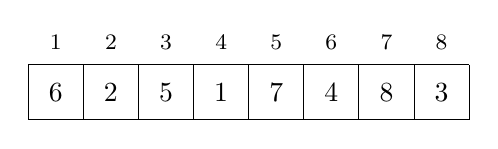
\begin{tikzpicture}[scale=0.7]
\draw (0,0) grid (8,1);
\node at (0.5,0.5) {$6$};
\node at (1.5,0.5) {$2$};
\node at (2.5,0.5) {$5$};
\node at (3.5,0.5) {$1$};
\node at (4.5,0.5) {$7$};
\node at (5.5,0.5) {$4$};
\node at (6.5,0.5) {$8$};
\node at (7.5,0.5) {$3$};

\footnotesize
\node at (0.5,1.4) {$1$};
\node at (1.5,1.4) {$2$};
\node at (2.5,1.4) {$3$};
\node at (3.5,1.4) {$4$};
\node at (4.5,1.4) {$5$};
\node at (5.5,1.4) {$6$};
\node at (6.5,1.4) {$7$};
\node at (7.5,1.4) {$8$};
\end{tikzpicture}
\end{center}
the longest increasing subsequence
contains 4 elements:
\begin{center}
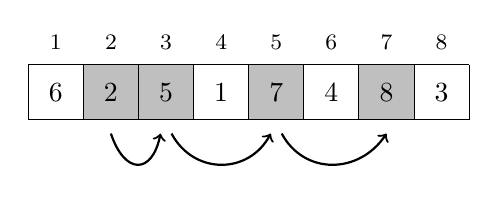
\begin{tikzpicture}[scale=0.7]
\fill[color=lightgray] (1,0) rectangle (2,1);
\fill[color=lightgray] (2,0) rectangle (3,1);
\fill[color=lightgray] (4,0) rectangle (5,1);
\fill[color=lightgray] (6,0) rectangle (7,1);
\draw (0,0) grid (8,1);
\node at (0.5,0.5) {$6$};
\node at (1.5,0.5) {$2$};
\node at (2.5,0.5) {$5$};
\node at (3.5,0.5) {$1$};
\node at (4.5,0.5) {$7$};
\node at (5.5,0.5) {$4$};
\node at (6.5,0.5) {$8$};
\node at (7.5,0.5) {$3$};

\draw[thick,->] (1.5,-0.25) .. controls (1.75,-1.00) and (2.25,-1.00) .. (2.4,-0.25);
\draw[thick,->] (2.6,-0.25) .. controls (3.0,-1.00) and (4.0,-1.00) .. (4.4,-0.25);
\draw[thick,->] (4.6,-0.25) .. controls (5.0,-1.00) and (6.0,-1.00) .. (6.5,-0.25);

\footnotesize
\node at (0.5,1.4) {$1$};
\node at (1.5,1.4) {$2$};
\node at (2.5,1.4) {$3$};
\node at (3.5,1.4) {$4$};
\node at (4.5,1.4) {$5$};
\node at (5.5,1.4) {$6$};
\node at (6.5,1.4) {$7$};
\node at (7.5,1.4) {$8$};
\end{tikzpicture}
\end{center}

Let $f(k)$ be the length of the
longest increasing subsequence
that ends at position $k$.
Using this function, the answer to the problem
is the largest of the values
$f(1),f(2),\ldots,f(n)$.
For example, in the above array
the values of the function are as follows:
\[
\begin{array}{lcl}
f(1) & = & 1 \\
f(2) & = & 1 \\
f(3) & = & 2 \\
f(4) & = & 1 \\
f(5) & = & 3 \\
f(6) & = & 2 \\
f(7) & = & 4 \\
f(8) & = & 2 \\
\end{array}
\]

When calculating the value of $f(k)$,
there are two possibilities how the subsequence
that ends at position $k$ is constructed:
\begin{enumerate}
\item The subsequence
only contains the element $x_k$. In this case $f(k)=1$.
\item The subsequence is constructed
by adding the element $x_k$ to
a subsequence that ends at position $i$
where $i<k$ and $x_i<x_k$. In this case $f(k)=f(i)+1$.
\end{enumerate}

For example, in the above example $f(7)=4$,
because the subsequence $[2,5,7]$ of length 3
ends at position 5, and by adding the element
at position 7 to this subsequence,
we get the optimal subsequence $[2,5,7,8]$ of length 4.

An easy way to calculate the
value of $f(k)$ is to
go through all previous values
$f(1),f(2),\ldots,f(k-1)$ and select the best solution.
The time complexity of such an algorithm is $O(n^2)$.
Surprisingly, it is also possible to solve the
problem in $O(n \log n)$ time. Can you see how?

\section{Paths in a grid}

Our next problem is to find a path
in an $n \times n$ grid
from the upper-left corner to
the lower-right corner such that
we only move down and right.
Each square contains a number,
and the path should be constructed so
that the sum of numbers along
the path is as large as possible.

The following picture shows an optimal
path in a grid:
\begin{center}
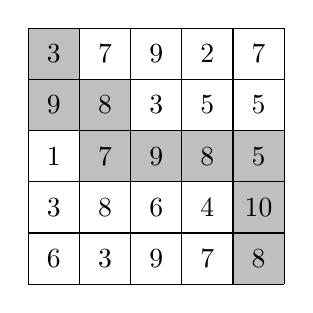
\begin{tikzpicture}[scale=.65]
  \begin{scope}
    \fill [color=lightgray] (0, 9) rectangle (1, 8);
    \fill [color=lightgray] (0, 8) rectangle (1, 7);
    \fill [color=lightgray] (1, 8) rectangle (2, 7);
    \fill [color=lightgray] (1, 7) rectangle (2, 6);
    \fill [color=lightgray] (2, 7) rectangle (3, 6);
    \fill [color=lightgray] (3, 7) rectangle (4, 6);
    \fill [color=lightgray] (4, 7) rectangle (5, 6);
    \fill [color=lightgray] (4, 6) rectangle (5, 5);
    \fill [color=lightgray] (4, 5) rectangle (5, 4);
    \draw (0, 4) grid (5, 9);
    \node at (0.5,8.5) {3};
    \node at (1.5,8.5) {7};
    \node at (2.5,8.5) {9};
    \node at (3.5,8.5) {2};
    \node at (4.5,8.5) {7};
    \node at (0.5,7.5) {9};
    \node at (1.5,7.5) {8};
    \node at (2.5,7.5) {3};
    \node at (3.5,7.5) {5};
    \node at (4.5,7.5) {5};
    \node at (0.5,6.5) {1};
    \node at (1.5,6.5) {7};
    \node at (2.5,6.5) {9};
    \node at (3.5,6.5) {8};
    \node at (4.5,6.5) {5};
    \node at (0.5,5.5) {3};
    \node at (1.5,5.5) {8};
    \node at (2.5,5.5) {6};
    \node at (3.5,5.5) {4};
    \node at (4.5,5.5) {10};
    \node at (0.5,4.5) {6};
    \node at (1.5,4.5) {3};
    \node at (2.5,4.5) {9};
    \node at (3.5,4.5) {7};
    \node at (4.5,4.5) {8};
  \end{scope}
\end{tikzpicture}
\end{center}
The sum of numbers on the path is 67,
and this is the largest possible sum on a path
from the
upper-left corner to the lower-right corner.

We can approach the problem by
calculating for each square $(y,x)$
the maximum sum on a path
from the upper-left corner to square $(y,x)$.
Let $f(y,x)$ denote this sum,
so $f(n,n)$ is the maximum sum on a path
from the upper-left corner to
the lower-right corner.

The recursive formula is based on the observation
that a path that ends at square $(y,x)$
can come either from square $(y,x-1)$
or square $(y-1,x)$:
\begin{center}
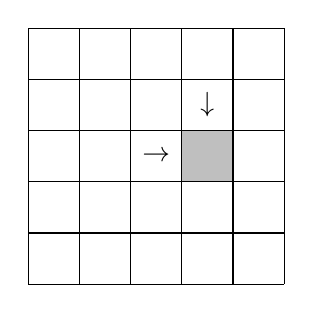
\begin{tikzpicture}[scale=.65]
  \begin{scope}
    \fill [color=lightgray] (3, 7) rectangle (4, 6);
    \draw (0, 4) grid (5, 9);
    
    \node at (2.5,6.5) {$\rightarrow$};
    \node at (3.5,7.5) {$\downarrow$};
    
  \end{scope}
\end{tikzpicture}
\end{center}

Let $r(y,x)$ denote the number in square $(y,x)$.
The base cases for the recursive function
are as follows:

\[
\begin{array}{lcl}
f(1,1) & = & r(1,1) \\
f(1,x) & = & f(1,x-1)+r(1,x) \\
f(y,1) & = & f(y-1,1)+r(y,1)\\
\end{array}
\]

In the general case there are two
possible paths, and we should select the path
that produces the larger sum:
\[ f(y,x) = \max(f(y,x-1),f(y-1,x))+r(y,x)\]

The time complexity of the solution is $O(n^2)$,
because each value $f(y,x)$ can be calculated
in constant time using the values of the
adjacent squares.

\section{Knapsack}

\index{knapsack}

\key{Knapsack} is a classic problem where we
are given $n$ objects with weights
$p_1,p_2,\ldots,p_n$ and values
$a_1,a_2,\ldots,a_n$.
Our task is to choose a subset of the objects
such that the sum of the weights is at most $x$
and the sum of the values is as large as possible.

\begin{samepage}
For example, if the objects are
\begin{center}
\begin{tabular}{rrr}
object & weight & value \\
\hline
A & 5 & 1 \\
B & 6 & 3 \\
C & 8 & 5 \\
D & 5 & 3 \\
\end{tabular}
\end{center}
\end{samepage}
and the maximum allowed total weight is 12,
an optimal solution is to select objects $B$ and $D$.
Their total weight $6+5=11$ does not exceed 12,
and their total value $3+3=6$ is the largest possible.

This task can be solved in two different ways
using dynamic programming.
We can either regard the problem as maximizing the
total value of the objects or 
minimizing the total weight of the objects.

\subsubsection{Solution 1}

\textit{Maximization:} Let $f(k,u)$
denote the largest possible total value
when a subset of objects $1 \ldots k$ is selected
such that the total weight is $u$.
The solution to the problem is
the largest value
$f(n,u)$ where $0 \le u \le x$.
A recursive formula for calculating
the function is
\[f(k,u) = \max(f(k-1,u),f(k-1,u-p_k)+a_k),\]
because we can either include or not include
object $k$ in the solution.
The base cases are $f(0,0)=0$ and $f(0,u)=-\infty$
when $u \neq 0$. The time compexity of
the solution is $O(nx)$.

In the example case, the optimal solution is
$f(4,11)=6$ that can be constructed
using the following sequence:
\[f(4,11)=f(3,6)+3=f(2,6)+3=f(1,0)+3+3=f(0,0)+3+3=6.\]

\subsubsection{Solution 2}

\textit{Minimization:} Let $f(k,u)$
denote the smallest possible total weight
when a subset of objects
$1 \ldots k$ is selected such
that the total weight is $u$.
The solution to the problem is the
largest value $u$
for which  $0 \le u \le s$ and $f(n,u) \le x$
where $s=\sum_{i=1}^n a_i$.
A recursive formula for calculating the function is
\[f(k,u) = \min(f(k-1,u),f(k-1,u-a_k)+p_k)\]
as in solution 1.
The base cases are $f(0,0)=0$ and $f(0,u)=\infty$
when $u \neq 0$.
The time complexity of the solution is $O(ns)$.

In the example case, the optimal solution is $f(4,6)=11$
that can be constructed using the following sequence:
\[f(4,6)=f(3,3)+5=f(2,3)+5=f(1,0)+6+5=f(0,0)+6+5=11.\]

~\\
It is interesting to note how the parameters of the input
affect the efficiency of the solutions.
The efficiency of solution 1 depends on the weights
of the objects, while the efficiency of solution 2
depends on the values of the objects.

\section{Edit distance}

\index{edit distance}
\index{Levenshtein distance}

The \key{edit distance} or \key{Levenshtein distance}
is the minimum number of editing operations
needed to transform a string
into another string.
The allowed editing operations are as follows:
\begin{itemize}
\item insert a character (e.g. \texttt{ABC} $\rightarrow$ \texttt{ABCA})
\item remove a character (e.g. \texttt{ABC} $\rightarrow$ \texttt{AC})
\item change a character (e.g. \texttt{ABC} $\rightarrow$ \texttt{ADC})
\end{itemize}

For example, the edit distance between
\texttt{LOVE} and \texttt{MOVIE} is 2,
because we can first perform the operation
 \texttt{LOVE} $\rightarrow$ \texttt{MOVE}
(change) and then the operation
\texttt{MOVE} $\rightarrow$ \texttt{MOVIE}
(insertion).
This is the smallest possible number of operations,
because it is clear that it is not possible
to use only one operation.

Suppose we are given strings
\texttt{x} and \texttt{y} that contain
$n$ and $m$ characters, respectively,
and we wish to calculate the edit distance
between them.
This can be done using
dynamic programming in $O(nm)$ time.
Let $f(a,b)$ denote the edit distance
between the first $a$ characters of \texttt{x}
and the first $b$ characters of \texttt{y}.
Using this function, the edit distance between
\texttt{x} and \texttt{y} equals $f(n,m)$.

The base cases for the function are
\[
\begin{array}{lcl}
f(0,b) & = & b \\
f(a,0) & = & a \\
\end{array}
\]
and in the general case the formula is
\[ f(a,b) = \min(f(a,b-1)+1,f(a-1,b)+1,f(a-1,b-1)+c),\]
where $c=0$ if the $a$th character of \texttt{x}
equals the $b$th character of \texttt{y},
and otherwise $c=1$.
The formula considers all possible ways to shorten the strings:
\begin{itemize}
\item $f(a,b-1)$ means that a character is inserted to \texttt{x}
\item $f(a-1,b)$ means that a character is removed from \texttt{x}
\item $f(a-1,b-1)$ means that \texttt{x} and \texttt{y} contain
the same character ($c=0$),
or a character in \texttt{x} is transformed into
a character in \texttt{y} ($c=1$)
\end{itemize}
The following table shows the values of $f$
in the example case:
\begin{center}
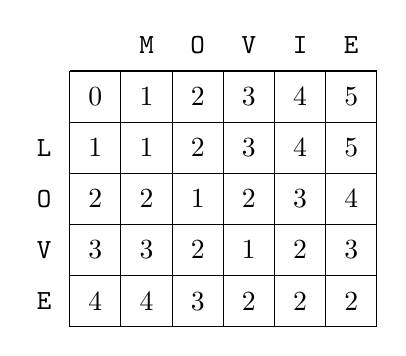
\begin{tikzpicture}[scale=.65]
  \begin{scope}
    %\fill [color=lightgray] (5, -3) rectangle (6, -4);
    \draw (1, -1) grid (7, -6);
    
    \node at (0.5,-2.5) {\texttt{L}};
    \node at (0.5,-3.5) {\texttt{O}};
    \node at (0.5,-4.5) {\texttt{V}};
    \node at (0.5,-5.5) {\texttt{E}};

    \node at (2.5,-0.5) {\texttt{M}};
    \node at (3.5,-0.5) {\texttt{O}};
    \node at (4.5,-0.5) {\texttt{V}};
    \node at (5.5,-0.5) {\texttt{I}};
    \node at (6.5,-0.5) {\texttt{E}};

    \node at (1.5,-1.5) {$0$};
    \node at (1.5,-2.5) {$1$};
    \node at (1.5,-3.5) {$2$};
    \node at (1.5,-4.5) {$3$};
    \node at (1.5,-5.5) {$4$};
    \node at (2.5,-1.5) {$1$};
    \node at (2.5,-2.5) {$1$};
    \node at (2.5,-3.5) {$2$};
    \node at (2.5,-4.5) {$3$};
    \node at (2.5,-5.5) {$4$};
    \node at (3.5,-1.5) {$2$};
    \node at (3.5,-2.5) {$2$};
    \node at (3.5,-3.5) {$1$};
    \node at (3.5,-4.5) {$2$};
    \node at (3.5,-5.5) {$3$};
    \node at (4.5,-1.5) {$3$};
    \node at (4.5,-2.5) {$3$};
    \node at (4.5,-3.5) {$2$};
    \node at (4.5,-4.5) {$1$};
    \node at (4.5,-5.5) {$2$};
    \node at (5.5,-1.5) {$4$};
    \node at (5.5,-2.5) {$4$};
    \node at (5.5,-3.5) {$3$};
    \node at (5.5,-4.5) {$2$};
    \node at (5.5,-5.5) {$2$};
    \node at (6.5,-1.5) {$5$};
    \node at (6.5,-2.5) {$5$};
    \node at (6.5,-3.5) {$4$};
    \node at (6.5,-4.5) {$3$};
    \node at (6.5,-5.5) {$2$};
  \end{scope}
\end{tikzpicture}
\end{center}

The lower-right corner of the table
tells us that the edit distance between
\texttt{LOVE} and \texttt{MOVIE} is 2.
The table also shows how to construct
the shortest sequence of editing operations.
In this case the path is as follows:

\begin{center}
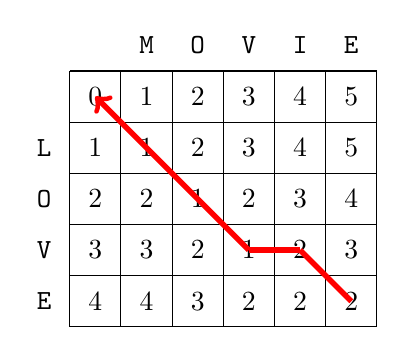
\begin{tikzpicture}[scale=.65]
  \begin{scope}
    \draw (1, -1) grid (7, -6);
    
    \node at (0.5,-2.5) {\texttt{L}};
    \node at (0.5,-3.5) {\texttt{O}};
    \node at (0.5,-4.5) {\texttt{V}};
    \node at (0.5,-5.5) {\texttt{E}};

    \node at (2.5,-0.5) {\texttt{M}};
    \node at (3.5,-0.5) {\texttt{O}};
    \node at (4.5,-0.5) {\texttt{V}};
    \node at (5.5,-0.5) {\texttt{I}};
    \node at (6.5,-0.5) {\texttt{E}};

    \node at (1.5,-1.5) {$0$};
    \node at (1.5,-2.5) {$1$};
    \node at (1.5,-3.5) {$2$};
    \node at (1.5,-4.5) {$3$};
    \node at (1.5,-5.5) {$4$};
    \node at (2.5,-1.5) {$1$};
    \node at (2.5,-2.5) {$1$};
    \node at (2.5,-3.5) {$2$};
    \node at (2.5,-4.5) {$3$};
    \node at (2.5,-5.5) {$4$};
    \node at (3.5,-1.5) {$2$};
    \node at (3.5,-2.5) {$2$};
    \node at (3.5,-3.5) {$1$};
    \node at (3.5,-4.5) {$2$};
    \node at (3.5,-5.5) {$3$};
    \node at (4.5,-1.5) {$3$};
    \node at (4.5,-2.5) {$3$};
    \node at (4.5,-3.5) {$2$};
    \node at (4.5,-4.5) {$1$};
    \node at (4.5,-5.5) {$2$};
    \node at (5.5,-1.5) {$4$};
    \node at (5.5,-2.5) {$4$};
    \node at (5.5,-3.5) {$3$};
    \node at (5.5,-4.5) {$2$};
    \node at (5.5,-5.5) {$2$};
    \node at (6.5,-1.5) {$5$};
    \node at (6.5,-2.5) {$5$};
    \node at (6.5,-3.5) {$4$};
    \node at (6.5,-4.5) {$3$};
    \node at (6.5,-5.5) {$2$};

    \path[draw=red,thick,-,line width=2pt] (6.5,-5.5) -- (5.5,-4.5);
    \path[draw=red,thick,-,line width=2pt] (5.5,-4.5) -- (4.5,-4.5);
    \path[draw=red,thick,->,line width=2pt] (4.5,-4.5) -- (1.5,-1.5);
  \end{scope}
\end{tikzpicture}
\end{center}

The last characters of \texttt{LOVE} and \texttt{MOVIE}
are equal, so the edit distance between them
equals the edit distance between \texttt{LOV} and \texttt{MOVI}.
We can use one editing operation to remove the
character \texttt{I} from \texttt{MOVI}.
Thus, the edit distance is one larger than
the edit distance between \texttt{LOV} and \texttt{MOV}, etc.

\section{Counting tilings}

Sometimes the states of a dynamic programming solution
are more complex than fixed combinations of numbers.
As an example,
we consider the problem of calculating
the number of distinct ways to
fill an $n \times m$ grid using
$1 \times 2$ and $2 \times 1$ size tiles.
For example, one valid solution
for the $4 \times 7$ grid is
\begin{center}
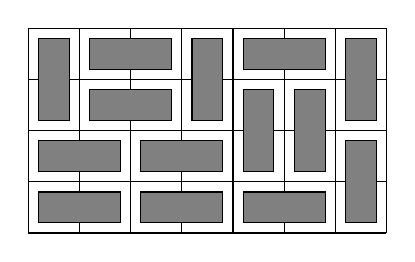
\begin{tikzpicture}[scale=.65]
    \draw (0,0) grid (7,4);
    \draw[fill=gray] (0+0.2,0+0.2) rectangle (2-0.2,1-0.2);
    \draw[fill=gray] (2+0.2,0+0.2) rectangle (4-0.2,1-0.2);
    \draw[fill=gray] (4+0.2,0+0.2) rectangle (6-0.2,1-0.2);
    \draw[fill=gray] (0+0.2,1+0.2) rectangle (2-0.2,2-0.2);
    \draw[fill=gray] (2+0.2,1+0.2) rectangle (4-0.2,2-0.2);
    \draw[fill=gray] (1+0.2,2+0.2) rectangle (3-0.2,3-0.2);
    \draw[fill=gray] (1+0.2,3+0.2) rectangle (3-0.2,4-0.2);
    \draw[fill=gray] (4+0.2,3+0.2) rectangle (6-0.2,4-0.2);

    \draw[fill=gray] (0+0.2,2+0.2) rectangle (1-0.2,4-0.2);
    \draw[fill=gray] (3+0.2,2+0.2) rectangle (4-0.2,4-0.2);
    \draw[fill=gray] (6+0.2,2+0.2) rectangle (7-0.2,4-0.2);
    \draw[fill=gray] (4+0.2,1+0.2) rectangle (5-0.2,3-0.2);
    \draw[fill=gray] (5+0.2,1+0.2) rectangle (6-0.2,3-0.2);
    \draw[fill=gray] (6+0.2,0+0.2) rectangle (7-0.2,2-0.2);

\end{tikzpicture}
\end{center}
and the total number of solutions is 781.

The problem can be solved using dynamic programming
by going through the grid row by row.
Each row in a solution can be represented as a
string that contains $m$ characters from the set
$\{\sqcap, \sqcup, \sqsubset, \sqsupset \}$.
For example, the above solution consists of four rows
that correspond to the following strings:
\begin{itemize}
\item
$\sqcap \sqsubset \sqsupset \sqcap \sqsubset \sqsupset \sqcap$
\item
$\sqcup \sqsubset \sqsupset \sqcup \sqcap \sqcap \sqcup$
\item
$\sqsubset \sqsupset \sqsubset \sqsupset \sqcup \sqcup \sqcap$ 
\item
$\sqsubset \sqsupset \sqsubset \sqsupset \sqsubset \sqsupset \sqcup$
\end{itemize}

Let $f(k,x)$ denote the number of ways to
construct a solution for rows $1 \ldots k$
in the grid so that string $x$ corresponds to row $k$.
It is possible to use dynamic programing here,
because the state of a row is constrained
only by the state of the previous row.

A solution is valid if row $1$ does not contain
the character $\sqcup$,
row $n$ does not contain the character $\sqcap$,
and all consecutive rows are \emph{compatible}.
For example, the rows
$\sqcup \sqsubset \sqsupset \sqcup \sqcap \sqcap \sqcup$ and
$\sqsubset \sqsupset \sqsubset \sqsupset \sqcup \sqcup \sqcap$ 
are compatible, while the rows
$\sqcap \sqsubset \sqsupset \sqcap \sqsubset \sqsupset \sqcap$ and
$\sqsubset \sqsupset \sqsubset \sqsupset \sqsubset \sqsupset \sqcup$
are not compatible.

Since a row consists of $m$ characters and there are
four choices for each character, the number of distinct
rows is at most $4^m$.
Thus, the time complexity of the solution is
$O(n 4^{2m})$ because we can go through the
$O(4^m)$ possible states for each row,
and for each state, there are $O(4^m)$
possible states for the previous row.
In practice, it is a good idea to rotate the grid
so that the shorter side has length $m$,
because the factor $4^{2m}$ dominates the time complexity.

It is possible to make the solution more efficient
by using a better representation for the rows.
It turns out that it is sufficient to know which
columns of the previous row contain the upper square
of a vertical tile.
Thus, we can represent a row using only characters
$\sqcap$ and $\Box$, where $\Box$ is a combination
of characters
$\sqcup$, $\sqsubset$ and $\sqsupset$.
Using this representation, there are only
$2^m$ distinct rows and the time complexity is
$O(n 2^{2m})$.

As a final note, there is also a surprising direct formula
for calculating the number of tilings:
\[ \prod_{a=1}^{\lceil n/2 \rceil} \prod_{b=1}^{\lceil m/2 \rceil} 4 \cdot (\cos^2 \frac{\pi a}{n + 1} + \cos^2 \frac{\pi b}{m+1})\]
This formula is very efficient, because it calculates
the number of tilings in $O(nm)$ time,
but since the answer is a product of real numbers,
a practical problem in using the formula is
how to store the intermediate results accurately.



\chapter{Amortized analysis}

\index{tasoitettu analyysi@tasoitettu analyysi}

Monen algoritmin aikavaativuuden pystyy laskemaan
suoraan katsomalla algoritmin rakennetta:
mitä silmukoita algoritmissa on ja miten monta
kertaa niitä suoritetaan.
Joskus kuitenkaan näin suoraviivainen analyysi ei
riitä antamaan todellista kuvaa algoritmin tehokkuudesta.

\key{Tasoitettu analyysi} soveltuu sellaisten
algoritmien analyysiin, joiden osana on jokin operaatio,
jonka ajankäyttö vaihtelee.
Ideana on tarkastella yksittäisen operaation
sijasta kaikkia operaatioita algoritmin
aikana ja laskea niiden ajankäytölle yhteinen raja.

\section{Kahden osoittimen tekniikka}

\index{kahden osoittimen tekniikka}

\key{Kahden osoittimen tekniikka} on taulukon käsittelyssä
käytettävä menetelmä, jossa taulukkoa käydään läpi
kahden osoittimen avulla.
Molemmat osoittimet liikkuvat algoritmin aikana,
mutta rajoituksena on, että ne voivat liikkua vain
yhteen suuntaan, mikä takaa, että algoritmi toimii tehokkaasti.

Tutustumme seuraavaksi kahden osoittimen tekniikkaan
kahden esimerkkitehtävän kautta.

\subsubsection{Alitaulukon summa}

Annettuna on taulukko, jossa on $n$ positiivista kokonaislukua.
Tehtävänä on selvittää, onko taulukossa alitaulukkoa,
jossa lukujen summa on $x$.
Esimerkiksi taulukossa
\begin{center}
\begin{tikzpicture}[scale=0.7]
\draw (0,0) grid (8,1);

\node at (0.5,0.5) {$1$};
\node at (1.5,0.5) {$3$};
\node at (2.5,0.5) {$2$};
\node at (3.5,0.5) {$5$};
\node at (4.5,0.5) {$1$};
\node at (5.5,0.5) {$1$};
\node at (6.5,0.5) {$2$};
\node at (7.5,0.5) {$3$};

\footnotesize
\node at (0.5,1.4) {$1$};
\node at (1.5,1.4) {$2$};
\node at (2.5,1.4) {$3$};
\node at (3.5,1.4) {$4$};
\node at (4.5,1.4) {$5$};
\node at (5.5,1.4) {$6$};
\node at (6.5,1.4) {$7$};
\node at (7.5,1.4) {$8$};
\end{tikzpicture}
\end{center}
on alitaulukko, jossa lukujen summa on 8:
\begin{center}
\begin{tikzpicture}[scale=0.7]
\fill[color=lightgray] (2,0) rectangle (5,1);
\draw (0,0) grid (8,1);

\node at (0.5,0.5) {$1$};
\node at (1.5,0.5) {$3$};
\node at (2.5,0.5) {$2$};
\node at (3.5,0.5) {$5$};
\node at (4.5,0.5) {$1$};
\node at (5.5,0.5) {$1$};
\node at (6.5,0.5) {$2$};
\node at (7.5,0.5) {$3$};

\footnotesize
\node at (0.5,1.4) {$1$};
\node at (1.5,1.4) {$2$};
\node at (2.5,1.4) {$3$};
\node at (3.5,1.4) {$4$};
\node at (4.5,1.4) {$5$};
\node at (5.5,1.4) {$6$};
\node at (6.5,1.4) {$7$};
\node at (7.5,1.4) {$8$};
\end{tikzpicture}
\end{center}

Osoittautuu, että tämän tehtävän voi ratkaista
ajassa $O(n)$ kahden osoittimen tekniikalla.
Ideana on käydä taulukkoa läpi kahden osoittimen
avulla, jotka rajaavat välin taulukosta.
Joka vuorolla vasen osoitin liikkuu
yhden askeleen eteenpäin ja oikea osoitin
liikkuu niin kauan eteenpäin kuin summa on enintään $x$.
Jos välin summaksi tulee tarkalleen $x$, ratkaisu on löytynyt.

Tarkastellaan esimerkkinä algoritmin toimintaa
seuraavassa taulukossa, kun tavoitteena on muodostaa summa $x=8$:
\begin{center}
\begin{tikzpicture}[scale=0.7]
\draw (0,0) grid (8,1);

\node at (0.5,0.5) {$1$};
\node at (1.5,0.5) {$3$};
\node at (2.5,0.5) {$2$};
\node at (3.5,0.5) {$5$};
\node at (4.5,0.5) {$1$};
\node at (5.5,0.5) {$1$};
\node at (6.5,0.5) {$2$};
\node at (7.5,0.5) {$3$};

\footnotesize
\node at (0.5,1.4) {$1$};
\node at (1.5,1.4) {$2$};
\node at (2.5,1.4) {$3$};
\node at (3.5,1.4) {$4$};
\node at (4.5,1.4) {$5$};
\node at (5.5,1.4) {$6$};
\node at (6.5,1.4) {$7$};
\node at (7.5,1.4) {$8$};
\end{tikzpicture}
\end{center}

Aluksi osoittimet rajaavat taulukosta välin,
jonka summa on $1+3+2=6$.
Väli ei voi olla tätä suurempi,
koska seuraava luku 5 veisi summan yli $x$:n.

\begin{center}
\begin{tikzpicture}[scale=0.7]
\fill[color=lightgray] (0,0) rectangle (3,1);
\draw (0,0) grid (8,1);

\node at (0.5,0.5) {$1$};
\node at (1.5,0.5) {$3$};
\node at (2.5,0.5) {$2$};
\node at (3.5,0.5) {$5$};
\node at (4.5,0.5) {$1$};
\node at (5.5,0.5) {$1$};
\node at (6.5,0.5) {$2$};
\node at (7.5,0.5) {$3$};

\draw[thick,->] (0.5,-0.7) -- (0.5,-0.1);
\draw[thick,->] (2.5,-0.7) -- (2.5,-0.1);

\footnotesize
\node at (0.5,1.4) {$1$};
\node at (1.5,1.4) {$2$};
\node at (2.5,1.4) {$3$};
\node at (3.5,1.4) {$4$};
\node at (4.5,1.4) {$5$};
\node at (5.5,1.4) {$6$};
\node at (6.5,1.4) {$7$};
\node at (7.5,1.4) {$8$};
\end{tikzpicture}
\end{center}

Seuraavaksi vasen osoitin siirtyy askeleen eteenpäin.
Oikea osoitin säilyy paikallaan, koska muuten
summa kasvaisi liian suureksi.

\begin{center}
\begin{tikzpicture}[scale=0.7]
\fill[color=lightgray] (1,0) rectangle (3,1);
\draw (0,0) grid (8,1);

\node at (0.5,0.5) {$1$};
\node at (1.5,0.5) {$3$};
\node at (2.5,0.5) {$2$};
\node at (3.5,0.5) {$5$};
\node at (4.5,0.5) {$1$};
\node at (5.5,0.5) {$1$};
\node at (6.5,0.5) {$2$};
\node at (7.5,0.5) {$3$};

\draw[thick,->] (1.5,-0.7) -- (1.5,-0.1);
\draw[thick,->] (2.5,-0.7) -- (2.5,-0.1);

\footnotesize
\node at (0.5,1.4) {$1$};
\node at (1.5,1.4) {$2$};
\node at (2.5,1.4) {$3$};
\node at (3.5,1.4) {$4$};
\node at (4.5,1.4) {$5$};
\node at (5.5,1.4) {$6$};
\node at (6.5,1.4) {$7$};
\node at (7.5,1.4) {$8$};
\end{tikzpicture}
\end{center}

Vasen osoitin siirtyy taas askeleen eteenpäin
ja tällä kertaa oikea osoitin siirtyy kolme askelta
eteenpäin. Muodostuu summa $2+5+1=8$ eli taulukosta
on löytynyt väli, jonka lukujen summa on $x$.

\begin{center}
\begin{tikzpicture}[scale=0.7]
\fill[color=lightgray] (2,0) rectangle (5,1);
\draw (0,0) grid (8,1);

\node at (0.5,0.5) {$1$};
\node at (1.5,0.5) {$3$};
\node at (2.5,0.5) {$2$};
\node at (3.5,0.5) {$5$};
\node at (4.5,0.5) {$1$};
\node at (5.5,0.5) {$1$};
\node at (6.5,0.5) {$2$};
\node at (7.5,0.5) {$3$};

\draw[thick,->] (2.5,-0.7) -- (2.5,-0.1);
\draw[thick,->] (4.5,-0.7) -- (4.5,-0.1);

\footnotesize
\node at (0.5,1.4) {$1$};
\node at (1.5,1.4) {$2$};
\node at (2.5,1.4) {$3$};
\node at (3.5,1.4) {$4$};
\node at (4.5,1.4) {$5$};
\node at (5.5,1.4) {$6$};
\node at (6.5,1.4) {$7$};
\node at (7.5,1.4) {$8$};
\end{tikzpicture}
\end{center}

% Algoritmin toteutus näyttää seuraavalta:
% 
% \begin{lstlisting}
% int s = 0, b = 0;
% for (int a = 1; a <= n; a++) {
%     while (b<n && s+t[b+1] <= x) {
%         b++;
%         s += t[b];
%     }
%     if (s == x) {
%         // ratkaisu löytyi
%     }
%     s -= t[a];
% }
% \end{lstlisting}
% 
% Muuttujat $a$ ja $b$ sisältävät vasemman ja oikean
% osoittimen kohdan.
% Muuttuja $s$ taas laskee lukujen summan välillä.
% Joka askeleella $a$ liikkuu askeleen eteenpäin
% ja $b$ liikkuu niin kauan kuin summa on enintään $x$.

Algoritmin aikavaativuus riippuu siitä,
kauanko oikean osoittimen liikkuminen vie aikaa.
Tämä vaihtelee, koska oikea osoitin voi liikkua
minkä tahansa matkan eteenpäin taulukossa.
Kuitenkin oikea osoitin liikkuu \textit{yhteensä}
$O(n)$ askelta algoritmin aikana, koska se voi
liikkua vain eteenpäin.

Koska sekä vasen että oikea osoitin liikkuvat
$O(n)$ askelta algoritmin aikana,
algoritmin aikavaativuus on $O(n)$.

\subsubsection{Kahden luvun summa}

\index{2SUM-ongelma}

Annettuna on taulukko, jossa on $n$ kokonaislukua,
sekä kokonaisluku $x$.
Tehtävänä on etsiä taulukosta kaksi lukua,
joiden summa on $x$, tai todeta,
että tämä ei ole mahdollista.
Tämä ongelma tunnetaan tunnetaan nimellä
\key{2SUM} ja se ratkeaa tehokkaasti
kahden osoittimen tekniikalla.

Taulukon luvut järjestetään ensin
pienimmästä suurimpaan, minkä jälkeen
taulukkoa aletaan käydä läpi kahdella osoittimella,
jotka lähtevät liikkelle taulukon molemmista päistä.
Vasen osoitin aloittaa taulukon alusta ja
liikkuu joka vaiheessa askeleen eteenpäin.
Oikea osoitin taas aloittaa taulukon lopusta
ja peruuttaa vuorollaan taaksepäin, kunnes osoitinten
määrittämän välin lukujen summa on enintään $x$.
Jos summa on tarkalleen $x$, ratkaisu on löytynyt.

Tarkastellaan algoritmin toimintaa
seuraavassa taulukossa, kun tavoitteena on muodostaa
summa $x=12$:
\begin{center}
\begin{tikzpicture}[scale=0.7]
\draw (0,0) grid (8,1);

\node at (0.5,0.5) {$1$};
\node at (1.5,0.5) {$4$};
\node at (2.5,0.5) {$5$};
\node at (3.5,0.5) {$6$};
\node at (4.5,0.5) {$7$};
\node at (5.5,0.5) {$9$};
\node at (6.5,0.5) {$9$};
\node at (7.5,0.5) {$10$};

\footnotesize
\node at (0.5,1.4) {$1$};
\node at (1.5,1.4) {$2$};
\node at (2.5,1.4) {$3$};
\node at (3.5,1.4) {$4$};
\node at (4.5,1.4) {$5$};
\node at (5.5,1.4) {$6$};
\node at (6.5,1.4) {$7$};
\node at (7.5,1.4) {$8$};
\end{tikzpicture}
\end{center}

Seuraavassa on algoritmin aloitustilanne.
Lukujen summa on $1+10=11$, joka on pienempi
kuin $x$:n arvo.

\begin{center}
\begin{tikzpicture}[scale=0.7]
\fill[color=lightgray] (0,0) rectangle (1,1);
\fill[color=lightgray] (7,0) rectangle (8,1);
\draw (0,0) grid (8,1);

\node at (0.5,0.5) {$1$};
\node at (1.5,0.5) {$4$};
\node at (2.5,0.5) {$5$};
\node at (3.5,0.5) {$6$};
\node at (4.5,0.5) {$7$};
\node at (5.5,0.5) {$9$};
\node at (6.5,0.5) {$9$};
\node at (7.5,0.5) {$10$};

\draw[thick,->] (0.5,-0.7) -- (0.5,-0.1);
\draw[thick,->] (7.5,-0.7) -- (7.5,-0.1);

\footnotesize
\node at (0.5,1.4) {$1$};
\node at (1.5,1.4) {$2$};
\node at (2.5,1.4) {$3$};
\node at (3.5,1.4) {$4$};
\node at (4.5,1.4) {$5$};
\node at (5.5,1.4) {$6$};
\node at (6.5,1.4) {$7$};
\node at (7.5,1.4) {$8$};
\end{tikzpicture}
\end{center}

Seuraavaksi vasen osoitin liikkuu askeleen eteenpäin.
Oikea osoitin peruuttaa kolme askelta, minkä jälkeen
summana on $4+7=11$.

\begin{center}
\begin{tikzpicture}[scale=0.7]
\fill[color=lightgray] (1,0) rectangle (2,1);
\fill[color=lightgray] (4,0) rectangle (5,1);
\draw (0,0) grid (8,1);

\node at (0.5,0.5) {$1$};
\node at (1.5,0.5) {$4$};
\node at (2.5,0.5) {$5$};
\node at (3.5,0.5) {$6$};
\node at (4.5,0.5) {$7$};
\node at (5.5,0.5) {$9$};
\node at (6.5,0.5) {$9$};
\node at (7.5,0.5) {$10$};

\draw[thick,->] (1.5,-0.7) -- (1.5,-0.1);
\draw[thick,->] (4.5,-0.7) -- (4.5,-0.1);

\footnotesize
\node at (0.5,1.4) {$1$};
\node at (1.5,1.4) {$2$};
\node at (2.5,1.4) {$3$};
\node at (3.5,1.4) {$4$};
\node at (4.5,1.4) {$5$};
\node at (5.5,1.4) {$6$};
\node at (6.5,1.4) {$7$};
\node at (7.5,1.4) {$8$};
\end{tikzpicture}
\end{center}

Sitten vasen osoitin siirtyy jälleen askeleen eteenpäin.
Oikea osoitin pysyy paikallaan ja ratkaisu $5+7=12$ on löytynyt.

\begin{center}
\begin{tikzpicture}[scale=0.7]
\fill[color=lightgray] (2,0) rectangle (3,1);
\fill[color=lightgray] (4,0) rectangle (5,1);
\draw (0,0) grid (8,1);

\node at (0.5,0.5) {$1$};
\node at (1.5,0.5) {$4$};
\node at (2.5,0.5) {$5$};
\node at (3.5,0.5) {$6$};
\node at (4.5,0.5) {$7$};
\node at (5.5,0.5) {$9$};
\node at (6.5,0.5) {$9$};
\node at (7.5,0.5) {$10$};

\draw[thick,->] (2.5,-0.7) -- (2.5,-0.1);
\draw[thick,->] (4.5,-0.7) -- (4.5,-0.1);

\footnotesize
\node at (0.5,1.4) {$1$};
\node at (1.5,1.4) {$2$};
\node at (2.5,1.4) {$3$};
\node at (3.5,1.4) {$4$};
\node at (4.5,1.4) {$5$};
\node at (5.5,1.4) {$6$};
\node at (6.5,1.4) {$7$};
\node at (7.5,1.4) {$8$};
\end{tikzpicture}
\end{center}

Algoritmin alussa taulukon järjestäminen vie
aikaa $O(n \log n)$.
Tämän jälkeen vasen osoitin liikkuu $O(n)$ askelta
eteenpäin ja oikea osoitin liikkuu $O(n)$ askelta
taaksepäin, mihin kuluu aikaa $O(n)$.
Algoritmin kokonaisaikavaativuus on siis $O(n \log n)$.

Huomaa, että tehtävän voi ratkaista myös 
toisella tavalla ajassa
$O(n \log n)$ binäärihaun avulla.
Tässä ratkaisussa jokaiselle taulukon luvulle
etsitään binäärihaulla toista lukua niin,
että lukujen summa olisi yhteensä $x$.
Binäärihaku suoritetaan $n$ kertaa ja
jokainen binäärihaku vie aikaa $O(\log n)$.

\index{3SUM-ongelma}
Hieman vaikeampi ongelma on \key{3SUM},
jossa taulukosta tuleekin etsiä kolme lukua,
joiden summa on $x$.
Tämä ongelma on mahdollista ratkaista ajassa $O(n^2)$.
Keksitkö, miten se tapahtuu?

\section{Lähin pienempi edeltäjä}

\index{lzhin pienempi edeltxjx@lähin pienempi edeltäjä}

Tasoitetun analyysin avulla arvioidaan usein
tietorakenteeseen kohdistuvien operaatioiden määrää.
Algoritmin operaatiot voivat jakautua epätasaisesti
niin, että useimmat operaatiot tehdään tietyssä
algoritmin vaiheessa, mutta operaatioiden
yhteismäärä on kuitenkin rajoitettu.

Tarkastellaan esimerkkinä ongelmaa,
jossa tehtävänä on etsiä kullekin taulukon
alkiolle
\key{lähin pienempi edeltäjä} eli
lähinnä oleva pienempi alkio taulukon alkuosassa.
On mahdollista, ettei tällaista alkiota ole olemassa,
jolloin algoritmin tulee huomata asia.
Osoittautuu, että tehtävä on mahdollista ratkaista
tehokkaasti ajassa $O(n)$ sopivan tietorakenteen avulla.

Tehokas ratkaisu tehtävään on käydä
taulukko läpi alusta loppuun ja pitää samalla yllä ketjua,
jonka ensimmäinen luku on käsiteltävä taulukon luku
ja jokainen seuraava luku on luvun lähin
pienempi edeltäjä.
Jos ketjussa on vain yksi luku,
käsiteltävällä luvulla ei ole pienempää edeltäjää.
Joka askeleella ketjun alusta poistetaan lukuja
niin kauan, kunnes ketjun ensimmäinen luku on 
pienempi kuin käsiteltävä taulukon luku tai ketju on tyhjä.
Tämän jälkeen käsiteltävä luku lisätään ketjun alkuun.

Tarkastellaan esimerkkinä algoritmin toimintaa
seuraavassa taulukossa:
\begin{center}
\begin{tikzpicture}[scale=0.7]
\draw (0,0) grid (8,1);

\node at (0.5,0.5) {$1$};
\node at (1.5,0.5) {$3$};
\node at (2.5,0.5) {$4$};
\node at (3.5,0.5) {$2$};
\node at (4.5,0.5) {$5$};
\node at (5.5,0.5) {$3$};
\node at (6.5,0.5) {$4$};
\node at (7.5,0.5) {$2$};

\footnotesize
\node at (0.5,1.4) {$1$};
\node at (1.5,1.4) {$2$};
\node at (2.5,1.4) {$3$};
\node at (3.5,1.4) {$4$};
\node at (4.5,1.4) {$5$};
\node at (5.5,1.4) {$6$};
\node at (6.5,1.4) {$7$};
\node at (7.5,1.4) {$8$};
\end{tikzpicture}
\end{center}

Aluksi luvut 1, 3 ja 4 liittyvät ketjuun, koska jokainen luku on
edellistä suurempi. Siis luvun 4 lähin pienempi edeltäjä on luku 3,
jonka lähin pienempi edeltäjä on puolestaan luku 1. Tilanne näyttää tältä:
\begin{center}
\begin{tikzpicture}[scale=0.7]
\fill[color=lightgray] (2,0) rectangle (3,1);
\draw (0,0) grid (8,1);

\node at (0.5,0.5) {$1$};
\node at (1.5,0.5) {$3$};
\node at (2.5,0.5) {$4$};
\node at (3.5,0.5) {$2$};
\node at (4.5,0.5) {$5$};
\node at (5.5,0.5) {$3$};
\node at (6.5,0.5) {$4$};
\node at (7.5,0.5) {$2$};

\draw[thick,->] (2.5,-0.25) .. controls (2.25,-1.00) and (1.75,-1.00) .. (1.6,-0.25);
\draw[thick,->] (1.4,-0.25) .. controls (1.25,-1.00) and (0.75,-1.00) .. (0.5,-0.25);

\footnotesize
\node at (0.5,1.4) {$1$};
\node at (1.5,1.4) {$2$};
\node at (2.5,1.4) {$3$};
\node at (3.5,1.4) {$4$};
\node at (4.5,1.4) {$5$};
\node at (5.5,1.4) {$6$};
\node at (6.5,1.4) {$7$};
\node at (7.5,1.4) {$8$};
\end{tikzpicture}
\end{center}

Taulukon seuraava luku 2 on pienempi kuin ketjun kaksi ensimmäistä lukua 4 ja 3.
Niinpä luvut 4 ja 3 poistetaan ketjusta, minkä jälkeen luku 2
lisätään ketjun alkuun. Sen lähin pienempi edeltäjä on luku 1:
\begin{center}
\begin{tikzpicture}[scale=0.7]
\fill[color=lightgray] (3,0) rectangle (4,1);
\draw (0,0) grid (8,1);

\node at (0.5,0.5) {$1$};
\node at (1.5,0.5) {$3$};
\node at (2.5,0.5) {$4$};
\node at (3.5,0.5) {$2$};
\node at (4.5,0.5) {$5$};
\node at (5.5,0.5) {$3$};
\node at (6.5,0.5) {$4$};
\node at (7.5,0.5) {$2$};

\draw[thick,->] (3.5,-0.25) .. controls (3.00,-1.00) and (1.00,-1.00) .. (0.5,-0.25);

\footnotesize
\node at (0.5,1.4) {$1$};
\node at (1.5,1.4) {$2$};
\node at (2.5,1.4) {$3$};
\node at (3.5,1.4) {$4$};
\node at (4.5,1.4) {$5$};
\node at (5.5,1.4) {$6$};
\node at (6.5,1.4) {$7$};
\node at (7.5,1.4) {$8$};
\end{tikzpicture}
\end{center}

Seuraava luku 5 on suurempi kuin luku 2,
joten se lisätään suoraan ketjun alkuun ja
sen lähin pienempi edeltäjä on luku 2:
\begin{center}
\begin{tikzpicture}[scale=0.7]
\fill[color=lightgray] (4,0) rectangle (5,1);
\draw (0,0) grid (8,1);

\node at (0.5,0.5) {$1$};
\node at (1.5,0.5) {$3$};
\node at (2.5,0.5) {$4$};
\node at (3.5,0.5) {$2$};
\node at (4.5,0.5) {$5$};
\node at (5.5,0.5) {$3$};
\node at (6.5,0.5) {$4$};
\node at (7.5,0.5) {$2$};

\draw[thick,->] (3.4,-0.25) .. controls (3.00,-1.00) and (1.00,-1.00) .. (0.5,-0.25);
\draw[thick,->] (4.5,-0.25) .. controls (4.25,-1.00) and (3.75,-1.00) .. (3.6,-0.25);

\footnotesize
\node at (0.5,1.4) {$1$};
\node at (1.5,1.4) {$2$};
\node at (2.5,1.4) {$3$};
\node at (3.5,1.4) {$4$};
\node at (4.5,1.4) {$5$};
\node at (5.5,1.4) {$6$};
\node at (6.5,1.4) {$7$};
\node at (7.5,1.4) {$8$};
\end{tikzpicture}
\end{center}

Algoritmi jatkaa samalla tavalla taulukon loppuun
ja selvittää jokaisen luvun lähimmän
pienemmän edeltäjän.
Mutta kuinka tehokas algoritmi on?

Algoritmin tehokkuus riippuu siitä,
kauanko ketjun käsittelyyn kuluu aikaa yhteensä.
Jos uusi luku on suurempi kuin ketjun ensimmäinen
luku, se vain lisätään ketjun alkuun,
mikä on tehokasta.
Joskus taas ketjussa voi olla useita
suurempia lukuja, joiden poistaminen vie aikaa.
Oleellista on kuitenkin, että jokainen
taulukossa oleva luku liittyy
tarkalleen kerran ketjuun ja poistuu
korkeintaan kerran ketjusta.
Niinpä jokainen luku aiheuttaa $O(1)$
ketjuun liittyvää operaatiota
ja algoritmin kokonaisaikavaativuus on $O(n)$.

\section{Liukuvan ikkunan minimi}

\index{liukuva ikkuna}
\index{liukuvan ikkunan minimi@liukuvan ikkunan minimi}

\key{Liukuva ikkuna} on taulukon halki kulkeva
aktiivinen alitaulukko, jonka pituus on vakio.
Jokaisessa liukuvan ikkunan sijainnissa
halutaan tyypillisesti laskea jotain tietoa
ikkunan alueelle osuvista alkioista.
Kiinnostava tehtävä on pitää yllä
\key{liukuvan ikkunan minimiä}.
Tämä tarkoittaa, että jokaisessa liukuvan ikkunan
sijainnissa tulee ilmoittaa pienin alkio
ikkunan alueella.

Liukuvan ikkunan minimit voi laskea
lähes samalla tavalla kuin lähimmät
pienimmät edeltäjät.
Ideana on pitää yllä ketjua, jonka alussa
on ikkunan viimeinen luku ja jossa jokainen
luku on edellistä pienempi. Joka vaiheessa
ketjun viimeinen luku on ikkunan pienin luku.
Kun liukuva ikkuna liikkuu eteenpäin ja välille
tulee uusi luku, ketjusta poistetaan kaikki luvut,
jotka ovat uutta lukua suurempia.
Tämän jälkeen uusi luku lisätään ketjun alkuun.
Lisäksi jos ketjun viimeinen luku ei enää kuulu
välille, se poistetaan ketjusta.

Tarkastellaan esimerkkinä, kuinka algoritmi selvittää
minimit seuraavassa taulukossa,
kun ikkunan koko $k=4$.

\begin{center}
\begin{tikzpicture}[scale=0.7]
\draw (0,0) grid (8,1);

\node at (0.5,0.5) {$2$};
\node at (1.5,0.5) {$1$};
\node at (2.5,0.5) {$4$};
\node at (3.5,0.5) {$5$};
\node at (4.5,0.5) {$3$};
\node at (5.5,0.5) {$4$};
\node at (6.5,0.5) {$1$};
\node at (7.5,0.5) {$2$};

\footnotesize
\node at (0.5,1.4) {$1$};
\node at (1.5,1.4) {$2$};
\node at (2.5,1.4) {$3$};
\node at (3.5,1.4) {$4$};
\node at (4.5,1.4) {$5$};
\node at (5.5,1.4) {$6$};
\node at (6.5,1.4) {$7$};
\node at (7.5,1.4) {$8$};
\end{tikzpicture}
\end{center}

Liukuva ikkuna aloittaa matkansa taulukon vasemmasta reunasta.
Ensimmäisessä ikkunan sijainnissa pienin luku on 1:
\begin{center}
\begin{tikzpicture}[scale=0.7]
\fill[color=lightgray] (0,0) rectangle (4,1);
\draw (0,0) grid (8,1);

\node at (0.5,0.5) {$2$};
\node at (1.5,0.5) {$1$};
\node at (2.5,0.5) {$4$};
\node at (3.5,0.5) {$5$};
\node at (4.5,0.5) {$3$};
\node at (5.5,0.5) {$4$};
\node at (6.5,0.5) {$1$};
\node at (7.5,0.5) {$2$};

\footnotesize
\node at (0.5,1.4) {$1$};
\node at (1.5,1.4) {$2$};
\node at (2.5,1.4) {$3$};
\node at (3.5,1.4) {$4$};
\node at (4.5,1.4) {$5$};
\node at (5.5,1.4) {$6$};
\node at (6.5,1.4) {$7$};
\node at (7.5,1.4) {$8$};

\draw[thick,->] (3.5,-0.25) .. controls (3.25,-1.00) and (2.75,-1.00) .. (2.6,-0.25);
\draw[thick,->] (2.4,-0.25) .. controls (2.25,-1.00) and (1.75,-1.00) .. (1.5,-0.25);

\end{tikzpicture}
\end{center}

Kun ikkuna siirtyy eteenpäin, mukaan tulee luku 3,
joka on pienempi kuin luvut 5 ja 4 ketjun alussa.
Niinpä luvut 5 ja 4 poistuvat ketjusta ja luku 3
siirtyy sen alkuun. Pienin luku on edelleen 1.
\begin{center}
\begin{tikzpicture}[scale=0.7]
\fill[color=lightgray] (1,0) rectangle (5,1);
\draw (0,0) grid (8,1);

\node at (0.5,0.5) {$2$};
\node at (1.5,0.5) {$1$};
\node at (2.5,0.5) {$4$};
\node at (3.5,0.5) {$5$};
\node at (4.5,0.5) {$3$};
\node at (5.5,0.5) {$4$};
\node at (6.5,0.5) {$1$};
\node at (7.5,0.5) {$2$};

\footnotesize
\node at (0.5,1.4) {$1$};
\node at (1.5,1.4) {$2$};
\node at (2.5,1.4) {$3$};
\node at (3.5,1.4) {$4$};
\node at (4.5,1.4) {$5$};
\node at (5.5,1.4) {$6$};
\node at (6.5,1.4) {$7$};
\node at (7.5,1.4) {$8$};

\draw[thick,->] (4.5,-0.25) .. controls (4.25,-1.00) and (1.75,-1.00) .. (1.5,-0.25);

\end{tikzpicture}
\end{center}

Ikkuna siirtyy taas eteenpäin, minkä seurauksena pienin luku 1
putoaa pois ikkunasta. Niinpä se poistetaan ketjun lopusta
ja uusi pienin luku on 3. Lisäksi uusi ikkunaan tuleva luku 4
lisätään ketjun alkuun.
\begin{center}
\begin{tikzpicture}[scale=0.7]
\fill[color=lightgray] (2,0) rectangle (6,1);
\draw (0,0) grid (8,1);

\node at (0.5,0.5) {$2$};
\node at (1.5,0.5) {$1$};
\node at (2.5,0.5) {$4$};
\node at (3.5,0.5) {$5$};
\node at (4.5,0.5) {$3$};
\node at (5.5,0.5) {$4$};
\node at (6.5,0.5) {$1$};
\node at (7.5,0.5) {$2$};

\footnotesize
\node at (0.5,1.4) {$1$};
\node at (1.5,1.4) {$2$};
\node at (2.5,1.4) {$3$};
\node at (3.5,1.4) {$4$};
\node at (4.5,1.4) {$5$};
\node at (5.5,1.4) {$6$};
\node at (6.5,1.4) {$7$};
\node at (7.5,1.4) {$8$};

\draw[thick,->] (5.5,-0.25) .. controls (5.25,-1.00) and (4.75,-1.00) .. (4.5,-0.25);
\end{tikzpicture}
\end{center}

Seuraavaksi ikkunaan tuleva luku 1 on pienempi
kuin kaikki ketjussa olevat luvut.
Tämän seurauksena koko ketju tyhjentyy ja
siihen jää vain luku 1:
\begin{center}
\begin{tikzpicture}[scale=0.7]
\fill[color=lightgray] (3,0) rectangle (7,1);
\draw (0,0) grid (8,1);

\node at (0.5,0.5) {$2$};
\node at (1.5,0.5) {$1$};
\node at (2.5,0.5) {$4$};
\node at (3.5,0.5) {$5$};
\node at (4.5,0.5) {$3$};
\node at (5.5,0.5) {$4$};
\node at (6.5,0.5) {$1$};
\node at (7.5,0.5) {$2$};

\footnotesize
\node at (0.5,1.4) {$1$};
\node at (1.5,1.4) {$2$};
\node at (2.5,1.4) {$3$};
\node at (3.5,1.4) {$4$};
\node at (4.5,1.4) {$5$};
\node at (5.5,1.4) {$6$};
\node at (6.5,1.4) {$7$};
\node at (7.5,1.4) {$8$};

\fill[color=black] (6.5,-0.25) circle (0.1);

%\draw[thick,->] (5.5,-0.25) .. controls (5.25,-1.00) and (4.75,-1.00) .. (4.5,-0.25);
\end{tikzpicture}
\end{center}

Lopuksi ikkuna saapuu viimeiseen sijaintiinsa.
Luku 2 lisätään ketjun alkuun,
mutta ikkunan pienin luku on edelleen 1.
\begin{center}
\begin{tikzpicture}[scale=0.7]
\fill[color=lightgray] (4,0) rectangle (8,1);
\draw (0,0) grid (8,1);

\node at (0.5,0.5) {$2$};
\node at (1.5,0.5) {$1$};
\node at (2.5,0.5) {$4$};
\node at (3.5,0.5) {$5$};
\node at (4.5,0.5) {$3$};
\node at (5.5,0.5) {$4$};
\node at (6.5,0.5) {$1$};
\node at (7.5,0.5) {$2$};

\footnotesize
\node at (0.5,1.4) {$1$};
\node at (1.5,1.4) {$2$};
\node at (2.5,1.4) {$3$};
\node at (3.5,1.4) {$4$};
\node at (4.5,1.4) {$5$};
\node at (5.5,1.4) {$6$};
\node at (6.5,1.4) {$7$};
\node at (7.5,1.4) {$8$};

\draw[thick,->] (7.5,-0.25) .. controls (7.25,-1.00) and (6.75,-1.00) .. (6.5,-0.25);
\end{tikzpicture}
\end{center}

Tässäkin algoritmissa jokainen taulukon luku lisätään
ketjuun tarkalleen kerran ja poistetaan ketjusta korkeintaan kerran,
joko ketjun alusta tai ketjun lopusta.
Niinpä algoritmin kokonaisaikavaativuus on $O(n)$.




\chapter{Range queries}

\index{range query}
\index{sum query}
\index{minimum query}
\index{maximum query}

In this chapter, we discuss data structures
that allow us to efficiently answer range queries.
In a \key{range query}, we are given two indices
to an array, and our task is to calculate some
value based on the elements between the given indices.
Typical range queries are:
\begin{itemize}
\item \key{sum query}: calculate the sum of elements
\item \key{minimum query}: find the smallest element
\item \key{maximum query}: find the largest element
\end{itemize}
For example, consider the range $[4,7]$ in the following array:
\begin{center}
\begin{tikzpicture}[scale=0.7]
\fill[color=lightgray] (3,0) rectangle (7,1);
\draw (0,0) grid (8,1);

\node at (0.5,0.5) {$1$};
\node at (1.5,0.5) {$3$};
\node at (2.5,0.5) {$8$};
\node at (3.5,0.5) {$4$};
\node at (4.5,0.5) {$6$};
\node at (5.5,0.5) {$1$};
\node at (6.5,0.5) {$3$};
\node at (7.5,0.5) {$4$};

\footnotesize
\node at (0.5,1.4) {$1$};
\node at (1.5,1.4) {$2$};
\node at (2.5,1.4) {$3$};
\node at (3.5,1.4) {$4$};
\node at (4.5,1.4) {$5$};
\node at (5.5,1.4) {$6$};
\node at (6.5,1.4) {$7$};
\node at (7.5,1.4) {$8$};
\end{tikzpicture}
\end{center}
In this range, the sum of elements is $4+6+1+3=16$,
the minimum element is 1 and the maximum element is 6.

A simple way to process range queries is to
go through all elements in the range.
For example, the following function \texttt{sum}
calculates the sum of elements in a range
$[a,b]$ of an array $t$:

\begin{lstlisting}
int sum(int a, int b) {
    int s = 0;
    for (int i = a; i <= b; i++) {
        s += t[i];
    }
    return s;
}
\end{lstlisting}

The above function works in $O(n)$ time,
where $n$ is the number of elements in the array.
Thus, we can process $q$ queries in $O(nq)$
time using the function.
However, if both $n$ and $q$ are large, this approach
is slow, and it turns out that there are
ways to process range queries much more efficiently.

\section{Static array queries}

We first focus on a situation where
the array is \key{static}, i.e.,
the elements are never modified between the queries.
In this case, it suffices to construct
a static data structure that tells us
the answer for any possible query.

\subsubsection{Sum queries}

\index{sum array}

It turns out that we can easily process
sum queries on a static array,
because we can construct a data structure called
a \key{sum array}.
Each element in a sum array corresponds to
the sum of elements in the original array up to that position.

For example, consider the following array:
\begin{center}
\begin{tikzpicture}[scale=0.7]
%\fill[color=lightgray] (3,0) rectangle (7,1);
\draw (0,0) grid (8,1);

\node at (0.5,0.5) {$1$};
\node at (1.5,0.5) {$3$};
\node at (2.5,0.5) {$4$};
\node at (3.5,0.5) {$8$};
\node at (4.5,0.5) {$6$};
\node at (5.5,0.5) {$1$};
\node at (6.5,0.5) {$4$};
\node at (7.5,0.5) {$2$};

\footnotesize
\node at (0.5,1.4) {$1$};
\node at (1.5,1.4) {$2$};
\node at (2.5,1.4) {$3$};
\node at (3.5,1.4) {$4$};
\node at (4.5,1.4) {$5$};
\node at (5.5,1.4) {$6$};
\node at (6.5,1.4) {$7$};
\node at (7.5,1.4) {$8$};
\end{tikzpicture}
\end{center}
The corresponding sum array is as follows:
\begin{center}
\begin{tikzpicture}[scale=0.7]
%\fill[color=lightgray] (3,0) rectangle (7,1);
\draw (0,0) grid (8,1);

\node at (0.5,0.5) {$1$};
\node at (1.5,0.5) {$4$};
\node at (2.5,0.5) {$8$};
\node at (3.5,0.5) {$16$};
\node at (4.5,0.5) {$22$};
\node at (5.5,0.5) {$23$};
\node at (6.5,0.5) {$27$};
\node at (7.5,0.5) {$29$};


\footnotesize
\node at (0.5,1.4) {$1$};
\node at (1.5,1.4) {$2$};
\node at (2.5,1.4) {$3$};
\node at (3.5,1.4) {$4$};
\node at (4.5,1.4) {$5$};
\node at (5.5,1.4) {$6$};
\node at (6.5,1.4) {$7$};
\node at (7.5,1.4) {$8$};
\end{tikzpicture}
\end{center}
Let $\textrm{sum}(a,b)$ denote the sum of elements
in the range $[a,b]$.
Since the sum array contains all values
of the form $\textrm{sum}(1,k)$,
we can calculate any value of
$\textrm{sum}(a,b)$ in $O(1)$ time, because
\[ \textrm{sum}(a,b) = \textrm{sum}(1,b) - \textrm{sum}(1,a-1).\]
By defining $\textrm{sum}(1,0)=0$,
the above formula also holds when $a=1$.

For example, consider the range $[4,7]$:
\begin{center}
\begin{tikzpicture}[scale=0.7]
\fill[color=lightgray] (3,0) rectangle (7,1);
\draw (0,0) grid (8,1);

\node at (0.5,0.5) {$1$};
\node at (1.5,0.5) {$3$};
\node at (2.5,0.5) {$4$};
\node at (3.5,0.5) {$8$};
\node at (4.5,0.5) {$6$};
\node at (5.5,0.5) {$1$};
\node at (6.5,0.5) {$4$};
\node at (7.5,0.5) {$2$};

\footnotesize
\node at (0.5,1.4) {$1$};
\node at (1.5,1.4) {$2$};
\node at (2.5,1.4) {$3$};
\node at (3.5,1.4) {$4$};
\node at (4.5,1.4) {$5$};
\node at (5.5,1.4) {$6$};
\node at (6.5,1.4) {$7$};
\node at (7.5,1.4) {$8$};
\end{tikzpicture}
\end{center}
The sum in the range is $8+6+1+4=19$.
This sum can be calculated using
two values in the sum array:
\begin{center}
\begin{tikzpicture}[scale=0.7]
\fill[color=lightgray] (2,0) rectangle (3,1);
\fill[color=lightgray] (6,0) rectangle (7,1);
\draw (0,0) grid (8,1);

\node at (0.5,0.5) {$1$};
\node at (1.5,0.5) {$4$};
\node at (2.5,0.5) {$8$};
\node at (3.5,0.5) {$16$};
\node at (4.5,0.5) {$22$};
\node at (5.5,0.5) {$23$};
\node at (6.5,0.5) {$27$};
\node at (7.5,0.5) {$29$};


\footnotesize
\node at (0.5,1.4) {$1$};
\node at (1.5,1.4) {$2$};
\node at (2.5,1.4) {$3$};
\node at (3.5,1.4) {$4$};
\node at (4.5,1.4) {$5$};
\node at (5.5,1.4) {$6$};
\node at (6.5,1.4) {$7$};
\node at (7.5,1.4) {$8$};
\end{tikzpicture}
\end{center}
Thus, the sum in the range $[4,7]$ is $27-8=19$.

It is also possible to generalize this idea
to higher dimensions.
For example, we can construct a two-dimensional
sum array that can be used for calculating
the sum of any rectangular subarray in $O(1)$ time.
Each value in such an array is the sum of a subarray
that begins at the upper-left corner of the array.

\begin{samepage}
The following picture illustrates the idea:
\begin{center}
\begin{tikzpicture}[scale=0.54]
\draw[fill=lightgray] (3,2) rectangle (7,5);
\draw (0,0) grid (10,7);
%\draw[line width=2pt] (3,2) rectangle (7,5);
\node[anchor=center] at (6.5, 2.5) {$A$};
\node[anchor=center] at (2.5, 2.5) {$B$};
\node[anchor=center] at (6.5, 5.5) {$C$};
\node[anchor=center] at (2.5, 5.5) {$D$};
\end{tikzpicture}
\end{center}
\end{samepage}

The sum of the gray subarray can be calculated
using the formula
\[S(A) - S(B) - S(C) + S(D),\]
where $S(X)$ denotes the sum of a rectangular
subarray from the upper-left corner
to the position of $X$.

\subsubsection{Minimum queries}

Next we will see how we can
process range minimum queries in $O(1)$ time
after an $O(n \log n)$ time preprocessing\footnote{There are also
sophisticated techniques \cite{fis11} where the preprocessing time
is only $O(n)$, but such algorithms are not needed in
competitive programming.}.
Note that minimum and maximum queries can always
be processed using similar techniques,
so it suffices to focus on minimum queries.

Let $\textrm{rmq}(a,b)$ (''range minimum query'')
denote the minimum element in the range $[a,b]$.
The idea is to precalculate all values of $\textrm{rmq}(a,b)$
where $b-a+1$, the length of the range, is a power of two.
For example, for the array

\begin{center}
\begin{tikzpicture}[scale=0.7]
\draw (0,0) grid (8,1);

\node at (0.5,0.5) {$1$};
\node at (1.5,0.5) {$3$};
\node at (2.5,0.5) {$4$};
\node at (3.5,0.5) {$8$};
\node at (4.5,0.5) {$6$};
\node at (5.5,0.5) {$1$};
\node at (6.5,0.5) {$4$};
\node at (7.5,0.5) {$2$};

\footnotesize
\node at (0.5,1.4) {$1$};
\node at (1.5,1.4) {$2$};
\node at (2.5,1.4) {$3$};
\node at (3.5,1.4) {$4$};
\node at (4.5,1.4) {$5$};
\node at (5.5,1.4) {$6$};
\node at (6.5,1.4) {$7$};
\node at (7.5,1.4) {$8$};
\end{tikzpicture}
\end{center}
the following values will be calculated:

\begin{center}
\begin{tabular}{ccc}

\begin{tabular}{ccc}
$a$ & $b$ & $\textrm{rmq}(a,b)$ \\
\hline
1 & 1 & 1 \\
2 & 2 & 3 \\
3 & 3 & 4 \\
4 & 4 & 8 \\
5 & 5 & 6 \\
6 & 6 & 1 \\
7 & 7 & 4 \\
8 & 8 & 2 \\
\end{tabular}

&

\begin{tabular}{ccc}
$a$ & $b$ & $\textrm{rmq}(a,b)$ \\
\hline
1 & 2 & 1 \\
2 & 3 & 3 \\
3 & 4 & 4 \\
4 & 5 & 6 \\
5 & 6 & 1 \\
6 & 7 & 1 \\
7 & 8 & 2 \\
\\
\end{tabular}

&

\begin{tabular}{ccc}
$a$ & $b$ & $\textrm{rmq}(a,b)$ \\
\hline
1 & 4 & 1 \\
2 & 5 & 3 \\
3 & 6 & 1 \\
4 & 7 & 1 \\
5 & 8 & 1 \\
1 & 8 & 1 \\
\\
\\
\end{tabular}

\end{tabular}
\end{center}

The number of precalculated values is $O(n \log n)$,
because there are $O(\log n)$ range lengths
that are powers of two.
In addition, the values can be calculated efficiently
using the recursive formula
\[\textrm{rmq}(a,b) = \min(\textrm{rmq}(a,a+w-1),\textrm{rmq}(a+w,b)),\]
where $b-a+1$ is a power of two and $w=(b-a+1)/2$.
Calculating all those values takes $O(n \log n)$ time.

After this, any value of $\textrm{rmq}(a,b)$ can be calculated
in $O(1)$ time as a minimum of two precalculated values.
Let $k$ be the largest power of two that does not exceed $b-a+1$.
We can calculate the value of $\textrm{rmq}(a,b)$ using the formula
\[\textrm{rmq}(a,b) = \min(\textrm{rmq}(a,a+k-1),\textrm{rmq}(b-k+1,b)).\]
In the above formula, the range $[a,b]$ is represented
as the union of the ranges $[a,a+k-1]$ and $[b-k+1,b]$, both of length $k$.

As an example, consider the range $[2,7]$:
\begin{center}
\begin{tikzpicture}[scale=0.7]
\fill[color=lightgray] (1,0) rectangle (7,1);
\draw (0,0) grid (8,1);

\node at (0.5,0.5) {$1$};
\node at (1.5,0.5) {$3$};
\node at (2.5,0.5) {$4$};
\node at (3.5,0.5) {$8$};
\node at (4.5,0.5) {$6$};
\node at (5.5,0.5) {$1$};
\node at (6.5,0.5) {$4$};
\node at (7.5,0.5) {$2$};

\footnotesize
\node at (0.5,1.4) {$1$};
\node at (1.5,1.4) {$2$};
\node at (2.5,1.4) {$3$};
\node at (3.5,1.4) {$4$};
\node at (4.5,1.4) {$5$};
\node at (5.5,1.4) {$6$};
\node at (6.5,1.4) {$7$};
\node at (7.5,1.4) {$8$};
\end{tikzpicture}
\end{center}
The length of the range is 6,
and the largest power of two that does
not exceed 6 is 4.
Thus the range $[2,7]$ is
the union of the ranges $[2,5]$ and $[4,7]$:
\begin{center}
\begin{tikzpicture}[scale=0.7]
\fill[color=lightgray] (1,0) rectangle (5,1);
\draw (0,0) grid (8,1);

\node at (0.5,0.5) {$1$};
\node at (1.5,0.5) {$3$};
\node at (2.5,0.5) {$4$};
\node at (3.5,0.5) {$8$};
\node at (4.5,0.5) {$6$};
\node at (5.5,0.5) {$1$};
\node at (6.5,0.5) {$4$};
\node at (7.5,0.5) {$2$};

\footnotesize
\node at (0.5,1.4) {$1$};
\node at (1.5,1.4) {$2$};
\node at (2.5,1.4) {$3$};
\node at (3.5,1.4) {$4$};
\node at (4.5,1.4) {$5$};
\node at (5.5,1.4) {$6$};
\node at (6.5,1.4) {$7$};
\node at (7.5,1.4) {$8$};
\end{tikzpicture}
\end{center}
\begin{center}
\begin{tikzpicture}[scale=0.7]
\fill[color=lightgray] (3,0) rectangle (7,1);
\draw (0,0) grid (8,1);

\node at (0.5,0.5) {$1$};
\node at (1.5,0.5) {$3$};
\node at (2.5,0.5) {$4$};
\node at (3.5,0.5) {$8$};
\node at (4.5,0.5) {$6$};
\node at (5.5,0.5) {$1$};
\node at (6.5,0.5) {$4$};
\node at (7.5,0.5) {$2$};


\footnotesize
\node at (0.5,1.4) {$1$};
\node at (1.5,1.4) {$2$};
\node at (2.5,1.4) {$3$};
\node at (3.5,1.4) {$4$};
\node at (4.5,1.4) {$5$};
\node at (5.5,1.4) {$6$};
\node at (6.5,1.4) {$7$};
\node at (7.5,1.4) {$8$};
\end{tikzpicture}
\end{center}
Since $\textrm{rmq}(2,5)=3$ and $\textrm{rmq}(4,7)=1$,
we can conclude that $\textrm{rmq}(2,7)=1$.

\section{Binary indexed trees}

\index{binary indexed tree}
\index{Fenwick tree}

A \key{binary indexed tree} or \key{Fenwick tree} \cite{fen94}
can be seen as a dynamic variant of a sum array.
This data structure supports two $O(\log n)$ time operations:
calculating the sum of elements in a range
and modifying the value of an element.

The advantage of a binary indexed tree is
that it allows us to efficiently update
the array elements between the sum queries.
This would not be possible using a sum array,
because after each update, we should build the
whole sum array again in $O(n)$ time.

\subsubsection{Structure}

A binary indexed tree can be represented as an array
where the value at position $x$ 
equals the sum of elements in the range $[x-k+1,x]$,
where $k$ is the largest power of two that divides $x$.
For example, if $x=6$, then $k=2$, because 2 divides 6
but 4 does not divide 6.

\begin{samepage}
For example, consider the following array:
\begin{center}
\begin{tikzpicture}[scale=0.7]
\draw (0,0) grid (8,1);

\node at (0.5,0.5) {$1$};
\node at (1.5,0.5) {$3$};
\node at (2.5,0.5) {$4$};
\node at (3.5,0.5) {$8$};
\node at (4.5,0.5) {$6$};
\node at (5.5,0.5) {$1$};
\node at (6.5,0.5) {$4$};
\node at (7.5,0.5) {$2$};

\footnotesize
\node at (0.5,1.4) {$1$};
\node at (1.5,1.4) {$2$};
\node at (2.5,1.4) {$3$};
\node at (3.5,1.4) {$4$};
\node at (4.5,1.4) {$5$};
\node at (5.5,1.4) {$6$};
\node at (6.5,1.4) {$7$};
\node at (7.5,1.4) {$8$};
\end{tikzpicture}
\end{center}
\end{samepage}
\begin{samepage}
The corresponding binary indexed tree is as follows:
\begin{center}
\begin{tikzpicture}[scale=0.7]
\draw (0,0) grid (8,1);

\node at (0.5,0.5) {$1$};
\node at (1.5,0.5) {$4$};
\node at (2.5,0.5) {$4$};
\node at (3.5,0.5) {$16$};
\node at (4.5,0.5) {$6$};
\node at (5.5,0.5) {$7$};
\node at (6.5,0.5) {$4$};
\node at (7.5,0.5) {$29$};

\footnotesize
\node at (0.5,1.4) {$1$};
\node at (1.5,1.4) {$2$};
\node at (2.5,1.4) {$3$};
\node at (3.5,1.4) {$4$};
\node at (4.5,1.4) {$5$};
\node at (5.5,1.4) {$6$};
\node at (6.5,1.4) {$7$};
\node at (7.5,1.4) {$8$};
\end{tikzpicture}
\end{center}
\end{samepage}

For example, the value at position 6
in the binary indexed tree is 7,
because the sum of elements in the range $[5,6]$
of the array is $6+1=7$.

The following picture shows more clearly
how each value in the binary indexed tree
corresponds to a range in the array:

\begin{center}
\begin{tikzpicture}[scale=0.7]
%\fill[color=lightgray] (3,0) rectangle (7,1);
\draw (0,0) grid (8,1);

\node at (0.5,0.5) {$1$};
\node at (1.5,0.5) {$4$};
\node at (2.5,0.5) {$4$};
\node at (3.5,0.5) {$16$};
\node at (4.5,0.5) {$6$};
\node at (5.5,0.5) {$7$};
\node at (6.5,0.5) {$4$};
\node at (7.5,0.5) {$29$};

\footnotesize
\node at (0.5,1.4) {$1$};
\node at (1.5,1.4) {$2$};
\node at (2.5,1.4) {$3$};
\node at (3.5,1.4) {$4$};
\node at (4.5,1.4) {$5$};
\node at (5.5,1.4) {$6$};
\node at (6.5,1.4) {$7$};
\node at (7.5,1.4) {$8$};

\draw[->,thick] (0.5,-0.9) -- (0.5,-0.1);
\draw[->,thick] (2.5,-0.9) -- (2.5,-0.1);
\draw[->,thick] (4.5,-0.9) -- (4.5,-0.1);
\draw[->,thick] (6.5,-0.9) -- (6.5,-0.1);
\draw[->,thick] (1.5,-1.9) -- (1.5,-0.1);
\draw[->,thick] (5.5,-1.9) -- (5.5,-0.1);
\draw[->,thick] (3.5,-2.9) -- (3.5,-0.1);
\draw[->,thick] (7.5,-3.9) -- (7.5,-0.1);

\draw (0,-1) -- (1,-1) -- (1,-1.5) -- (0,-1.5) -- (0,-1);
\draw (2,-1) -- (3,-1) -- (3,-1.5) -- (2,-1.5) -- (2,-1);
\draw (4,-1) -- (5,-1) -- (5,-1.5) -- (4,-1.5) -- (4,-1);
\draw (6,-1) -- (7,-1) -- (7,-1.5) -- (6,-1.5) -- (6,-1);
\draw (0,-2) -- (2,-2) -- (2,-2.5) -- (0,-2.5) -- (0,-2);
\draw (4,-2) -- (6,-2) -- (6,-2.5) -- (4,-2.5) -- (4,-2);
\draw (0,-3) -- (4,-3) -- (4,-3.5) -- (0,-3.5) -- (0,-3);
\draw (0,-4) -- (8,-4) -- (8,-4.5) -- (0,-4.5) -- (0,-4);
\end{tikzpicture}
\end{center}

\subsubsection{Sum queries}

The values in the binary indexed tree
can be used to efficiently calculate
the sum of elements in any range $[1,k]$,
because such a range
can be divided into $O(\log n)$ ranges
whose sums are available in the binary indexed tree.

For example, the range $[1,7]$ corresponds to
the following values:
\begin{center}
\begin{tikzpicture}[scale=0.7]
%\fill[color=lightgray] (3,0) rectangle (7,1);
\draw (0,0) grid (8,1);

\node at (0.5,0.5) {$1$};
\node at (1.5,0.5) {$4$};
\node at (2.5,0.5) {$4$};
\node at (3.5,0.5) {$16$};
\node at (4.5,0.5) {$6$};
\node at (5.5,0.5) {$7$};
\node at (6.5,0.5) {$4$};
\node at (7.5,0.5) {$29$};

\footnotesize
\node at (0.5,1.4) {$1$};
\node at (1.5,1.4) {$2$};
\node at (2.5,1.4) {$3$};
\node at (3.5,1.4) {$4$};
\node at (4.5,1.4) {$5$};
\node at (5.5,1.4) {$6$};
\node at (6.5,1.4) {$7$};
\node at (7.5,1.4) {$8$};

\draw[->,thick] (0.5,-0.9) -- (0.5,-0.1);
\draw[->,thick] (2.5,-0.9) -- (2.5,-0.1);
\draw[->,thick] (4.5,-0.9) -- (4.5,-0.1);
\draw[->,thick] (6.5,-0.9) -- (6.5,-0.1);
\draw[->,thick] (1.5,-1.9) -- (1.5,-0.1);
\draw[->,thick] (5.5,-1.9) -- (5.5,-0.1);
\draw[->,thick] (3.5,-2.9) -- (3.5,-0.1);
\draw[->,thick] (7.5,-3.9) -- (7.5,-0.1);

\draw (0,-1) -- (1,-1) -- (1,-1.5) -- (0,-1.5) -- (0,-1);
\draw (2,-1) -- (3,-1) -- (3,-1.5) -- (2,-1.5) -- (2,-1);
\draw (4,-1) -- (5,-1) -- (5,-1.5) -- (4,-1.5) -- (4,-1);
\draw[fill=lightgray] (6,-1) -- (7,-1) -- (7,-1.5) -- (6,-1.5) -- (6,-1);
\draw (0,-2) -- (2,-2) -- (2,-2.5) -- (0,-2.5) -- (0,-2);
\draw[fill=lightgray] (4,-2) -- (6,-2) -- (6,-2.5) -- (4,-2.5) -- (4,-2);
\draw[fill=lightgray] (0,-3) -- (4,-3) -- (4,-3.5) -- (0,-3.5) -- (0,-3);
\draw (0,-4) -- (8,-4) -- (8,-4.5) -- (0,-4.5) -- (0,-4);
\end{tikzpicture}
\end{center}

Hence, the sum of elements in the range $[1,7]$ is $16+7+4=27$.

To calculate the sum of elements in any range $[a,b]$,
we can use the same trick that we used with sum arrays:
\[ \textrm{sum}(a,b) = \textrm{sum}(1,b) - \textrm{sum}(1,a-1).\]
Also in this case, only $O(\log n)$ values are needed.

\subsubsection{Array updates}

When a value in the array changes,
several values in the binary indexed tree should be updated.
For example, if the element at position 3 changes,
the sums of the following ranges change:
\begin{center}
\begin{tikzpicture}[scale=0.7]
%\fill[color=lightgray] (3,0) rectangle (7,1);
\draw (0,0) grid (8,1);

\node at (0.5,0.5) {$1$};
\node at (1.5,0.5) {$4$};
\node at (2.5,0.5) {$4$};
\node at (3.5,0.5) {$16$};
\node at (4.5,0.5) {$6$};
\node at (5.5,0.5) {$7$};
\node at (6.5,0.5) {$4$};
\node at (7.5,0.5) {$29$};

\footnotesize
\node at (0.5,1.4) {$1$};
\node at (1.5,1.4) {$2$};
\node at (2.5,1.4) {$3$};
\node at (3.5,1.4) {$4$};
\node at (4.5,1.4) {$5$};
\node at (5.5,1.4) {$6$};
\node at (6.5,1.4) {$7$};
\node at (7.5,1.4) {$8$};

\draw[->,thick] (0.5,-0.9) -- (0.5,-0.1);
\draw[->,thick] (2.5,-0.9) -- (2.5,-0.1);
\draw[->,thick] (4.5,-0.9) -- (4.5,-0.1);
\draw[->,thick] (6.5,-0.9) -- (6.5,-0.1);
\draw[->,thick] (1.5,-1.9) -- (1.5,-0.1);
\draw[->,thick] (5.5,-1.9) -- (5.5,-0.1);
\draw[->,thick] (3.5,-2.9) -- (3.5,-0.1);
\draw[->,thick] (7.5,-3.9) -- (7.5,-0.1);

\draw (0,-1) -- (1,-1) -- (1,-1.5) -- (0,-1.5) -- (0,-1);
\draw[fill=lightgray] (2,-1) -- (3,-1) -- (3,-1.5) -- (2,-1.5) -- (2,-1);
\draw (4,-1) -- (5,-1) -- (5,-1.5) -- (4,-1.5) -- (4,-1);
\draw (6,-1) -- (7,-1) -- (7,-1.5) -- (6,-1.5) -- (6,-1);
\draw (0,-2) -- (2,-2) -- (2,-2.5) -- (0,-2.5) -- (0,-2);
\draw (4,-2) -- (6,-2) -- (6,-2.5) -- (4,-2.5) -- (4,-2);
\draw[fill=lightgray] (0,-3) -- (4,-3) -- (4,-3.5) -- (0,-3.5) -- (0,-3);
\draw[fill=lightgray] (0,-4) -- (8,-4) -- (8,-4.5) -- (0,-4.5) -- (0,-4);
\end{tikzpicture}
\end{center}

Since each array element belongs to $O(\log n)$
ranges in the binary indexed tree,
it suffices to update $O(\log n)$ values.


\subsubsection{Implementation}

The operations of a binary indexed tree can be implemented
in an elegant and efficient way using bit operations.
The key fact needed is that $k \& -k$
isolates the last one bit of a number $k$.
For example, $26 \& -26=2$ because the number $26$
corresponds to 11010 and the number $2$ corresponds to 10.

It turns out that when processing a sum query,
the position $k$ in the binary indexed tree needs to be
decreased by $k \& -k$ at every step,
and when updating the array,
the position $k$ needs to be increased by $k \& -k$ at every step.

Suppose that the binary indexed tree is stored in an array \texttt{b}.
The following function calculates
the sum of elements in a range $[1,k]$:
\begin{lstlisting}
int sum(int k) {
    int s = 0;
    while (k >= 1) {
        s += b[k];
        k -= k&-k;
    }
    return s;
}
\end{lstlisting}

The following function increases the value
of the element at position $k$ by $x$
($x$ can be positive or negative):
\begin{lstlisting}
void add(int k, int x) {
    while (k <= n) {
        b[k] += x;
        k += k&-k;
    }
}
\end{lstlisting}

The time complexity of both the functions is
$O(\log n)$, because the functions access $O(\log n)$
values in the binary indexed tree, and each move
to the next position
takes $O(1)$ time using bit operations.

\section{Segment trees}

\index{segment tree}

A \key{segment tree} is a data structure
that supports two operations:
processing a range query and
modifying an element in the array.
Segment trees can support
sum queries, minimum and maximum queries and many other
queries so that both operations work in $O(\log n)$ time.

Compared to a binary indexed tree,
the advantage of a segment tree is that it is
a more general data structure.
While binary indexed trees only support
sum queries, segment trees also support other queries.
On the other hand, a segment tree requires more
memory and is a bit more difficult to implement.

\subsubsection{Structure}

A segment tree is a binary tree that
contains $2n-1$ nodes.
The nodes on the bottom level of the tree
correspond to the array elements,
and the other nodes
contain information needed for processing range queries.

Throughout the section, we assume that the size
of the array is a power of two and zero-based
indexing is used, because it is convenient to build
a segment tree for such an array.
If the size of the array is not a power of two,
we can always append extra elements to it.

We will first discuss segment trees that support sum queries.
As an example, consider the following array:
\begin{center}
\begin{tikzpicture}[scale=0.7]
\draw (0,0) grid (8,1);

\node at (0.5,0.5) {$5$};
\node at (1.5,0.5) {$8$};
\node at (2.5,0.5) {$6$};
\node at (3.5,0.5) {$3$};
\node at (4.5,0.5) {$2$};
\node at (5.5,0.5) {$7$};
\node at (6.5,0.5) {$2$};
\node at (7.5,0.5) {$6$};

\footnotesize
\node at (0.5,1.4) {$0$};
\node at (1.5,1.4) {$1$};
\node at (2.5,1.4) {$2$};
\node at (3.5,1.4) {$3$};
\node at (4.5,1.4) {$4$};
\node at (5.5,1.4) {$5$};
\node at (6.5,1.4) {$6$};
\node at (7.5,1.4) {$7$};
\end{tikzpicture}
\end{center}
The corresponding segment tree is as follows:
\begin{center}
\begin{tikzpicture}[scale=0.7]
\draw (0,0) grid (8,1);

\node[anchor=center] at (0.5, 0.5) {5};
\node[anchor=center] at (1.5, 0.5) {8};
\node[anchor=center] at (2.5, 0.5) {6};
\node[anchor=center] at (3.5, 0.5) {3};
\node[anchor=center] at (4.5, 0.5) {2};
\node[anchor=center] at (5.5, 0.5) {7};
\node[anchor=center] at (6.5, 0.5) {2};
\node[anchor=center] at (7.5, 0.5) {6};

\node[draw, circle] (a) at (1,2.5) {13};
\path[draw,thick,-] (a) -- (0.5,1);
\path[draw,thick,-] (a) -- (1.5,1);
\node[draw, circle,minimum size=22pt] (b) at (3,2.5) {9};
\path[draw,thick,-] (b) -- (2.5,1);
\path[draw,thick,-] (b) -- (3.5,1);
\node[draw, circle,minimum size=22pt] (c) at (5,2.5) {9};
\path[draw,thick,-] (c) -- (4.5,1);
\path[draw,thick,-] (c) -- (5.5,1);
\node[draw, circle,minimum size=22pt] (d) at (7,2.5) {8};
\path[draw,thick,-] (d) -- (6.5,1);
\path[draw,thick,-] (d) -- (7.5,1);

\node[draw, circle] (i) at (2,4.5) {22};
\path[draw,thick,-] (i) -- (a);
\path[draw,thick,-] (i) -- (b);
\node[draw, circle] (j) at (6,4.5) {17};
\path[draw,thick,-] (j) -- (c);
\path[draw,thick,-] (j) -- (d);

\node[draw, circle] (m) at (4,6.5) {39};
\path[draw,thick,-] (m) -- (i);
\path[draw,thick,-] (m) -- (j);
\end{tikzpicture}
\end{center}

Each internal node in the segment tree contains
information about a range of size $2^k$
in the original array.
In the above tree, the value of each internal
node is the sum of the corresponding array elements,
and it can be calculated as the sum of
the values of its left and right child node.

\subsubsection{Range queries}

The sum of elements in a given range
can be calculated as a sum of values in the segment tree.
For example, consider the following range:
\begin{center}
\begin{tikzpicture}[scale=0.7]
\fill[color=gray!50] (2,0) rectangle (8,1);
\draw (0,0) grid (8,1);

\node[anchor=center] at (0.5, 0.5) {5};
\node[anchor=center] at (1.5, 0.5) {8};
\node[anchor=center] at (2.5, 0.5) {6};
\node[anchor=center] at (3.5, 0.5) {3};
\node[anchor=center] at (4.5, 0.5) {2};
\node[anchor=center] at (5.5, 0.5) {7};
\node[anchor=center] at (6.5, 0.5) {2};
\node[anchor=center] at (7.5, 0.5) {6};
% 
% \footnotesize
% \node at (0.5,1.4) {$1$};
% \node at (1.5,1.4) {$2$};
% \node at (2.5,1.4) {$3$};
% \node at (3.5,1.4) {$4$};
% \node at (4.5,1.4) {$5$};
% \node at (5.5,1.4) {$6$};
% \node at (6.5,1.4) {$7$};
% \node at (7.5,1.4) {$8$};
\end{tikzpicture}
\end{center}
The sum of elements in the range is
$6+3+2+7+2+6=26$.
The following two nodes in the tree
correspond to the range:
\begin{center}
\begin{tikzpicture}[scale=0.7]
\draw (0,0) grid (8,1);

\node[anchor=center] at (0.5, 0.5) {5};
\node[anchor=center] at (1.5, 0.5) {8};
\node[anchor=center] at (2.5, 0.5) {6};
\node[anchor=center] at (3.5, 0.5) {3};
\node[anchor=center] at (4.5, 0.5) {2};
\node[anchor=center] at (5.5, 0.5) {7};
\node[anchor=center] at (6.5, 0.5) {2};
\node[anchor=center] at (7.5, 0.5) {6};

\node[draw, circle] (a) at (1,2.5) {13};
\path[draw,thick,-] (a) -- (0.5,1);
\path[draw,thick,-] (a) -- (1.5,1);
\node[draw, circle,fill=gray!50,minimum size=22pt] (b) at (3,2.5) {9};
\path[draw,thick,-] (b) -- (2.5,1);
\path[draw,thick,-] (b) -- (3.5,1);
\node[draw, circle,minimum size=22pt] (c) at (5,2.5) {9};
\path[draw,thick,-] (c) -- (4.5,1);
\path[draw,thick,-] (c) -- (5.5,1);
\node[draw, circle,minimum size=22pt] (d) at (7,2.5) {8};
\path[draw,thick,-] (d) -- (6.5,1);
\path[draw,thick,-] (d) -- (7.5,1);

\node[draw, circle] (i) at (2,4.5) {22};
\path[draw,thick,-] (i) -- (a);
\path[draw,thick,-] (i) -- (b);
\node[draw, circle,fill=gray!50] (j) at (6,4.5) {17};
\path[draw,thick,-] (j) -- (c);
\path[draw,thick,-] (j) -- (d);

\node[draw, circle] (m) at (4,6.5) {39};
\path[draw,thick,-] (m) -- (i);
\path[draw,thick,-] (m) -- (j);
\end{tikzpicture}
\end{center}
Thus, the sum of elements in the range is $9+17=26$.

When the sum is calculated using nodes
that are located as high as possible in the tree,
at most two nodes on each level
of the tree are needed.
Hence, the total number of nodes
is only $O(\log n)$.

\subsubsection{Array updates}

When an element in the array changes,
we should update all nodes in the tree
whose value depends on the element.
This can be done by traversing the path
from the element to the top node
and updating the nodes along the path.

\begin{samepage}
The following picture shows which nodes in the segment tree
change if the element 7 in the array changes.

\begin{center}
\begin{tikzpicture}[scale=0.7]
\fill[color=gray!50] (5,0) rectangle (6,1);
\draw (0,0) grid (8,1);

\node[anchor=center] at (0.5, 0.5) {5};
\node[anchor=center] at (1.5, 0.5) {8};
\node[anchor=center] at (2.5, 0.5) {6};
\node[anchor=center] at (3.5, 0.5) {3};
\node[anchor=center] at (4.5, 0.5) {2};
\node[anchor=center] at (5.5, 0.5) {7};
\node[anchor=center] at (6.5, 0.5) {2};
\node[anchor=center] at (7.5, 0.5) {6};

\node[draw, circle] (a) at (1,2.5) {13};
\path[draw,thick,-] (a) -- (0.5,1);
\path[draw,thick,-] (a) -- (1.5,1);
\node[draw, circle,minimum size=22pt] (b) at (3,2.5) {9};
\path[draw,thick,-] (b) -- (2.5,1);
\path[draw,thick,-] (b) -- (3.5,1);
\node[draw, circle,minimum size=22pt,fill=gray!50] (c) at (5,2.5) {9};
\path[draw,thick,-] (c) -- (4.5,1);
\path[draw,thick,-] (c) -- (5.5,1);
\node[draw, circle,minimum size=22pt] (d) at (7,2.5) {8};
\path[draw,thick,-] (d) -- (6.5,1);
\path[draw,thick,-] (d) -- (7.5,1);

\node[draw, circle] (i) at (2,4.5) {22};
\path[draw,thick,-] (i) -- (a);
\path[draw,thick,-] (i) -- (b);
\node[draw, circle,fill=gray!50] (j) at (6,4.5) {17};
\path[draw,thick,-] (j) -- (c);
\path[draw,thick,-] (j) -- (d);

\node[draw, circle,fill=gray!50] (m) at (4,6.5) {39};
\path[draw,thick,-] (m) -- (i);
\path[draw,thick,-] (m) -- (j);
\end{tikzpicture}
\end{center}
\end{samepage}

The path from bottom to top
always consists of $O(\log n)$ nodes,
so each update changes $O(\log n)$ nodes in the tree.

\subsubsection{Storing the tree}

A segment tree can be stored in an array
of $2N$ elements where $N$ is a power of two.
Such a tree corresponds to an array
indexed from $0$ to $N-1$.

In the segment tree array,
the element at position 1
corresponds to the top node of the tree,
the elements at positions 2 and 3 correspond to
the second level of the tree, and so on.
Finally, the elements at positions $N \ldots 2N-1$
correspond to the bottom level of the tree, i.e.,
the elements of the original array.

For example, the segment tree
\begin{center}
\begin{tikzpicture}[scale=0.7]
\draw (0,0) grid (8,1);

\node[anchor=center] at (0.5, 0.5) {5};
\node[anchor=center] at (1.5, 0.5) {8};
\node[anchor=center] at (2.5, 0.5) {6};
\node[anchor=center] at (3.5, 0.5) {3};
\node[anchor=center] at (4.5, 0.5) {2};
\node[anchor=center] at (5.5, 0.5) {7};
\node[anchor=center] at (6.5, 0.5) {2};
\node[anchor=center] at (7.5, 0.5) {6};

\node[draw, circle] (a) at (1,2.5) {13};
\path[draw,thick,-] (a) -- (0.5,1);
\path[draw,thick,-] (a) -- (1.5,1);
\node[draw, circle,minimum size=22pt] (b) at (3,2.5) {9};
\path[draw,thick,-] (b) -- (2.5,1);
\path[draw,thick,-] (b) -- (3.5,1);
\node[draw, circle,minimum size=22pt] (c) at (5,2.5) {9};
\path[draw,thick,-] (c) -- (4.5,1);
\path[draw,thick,-] (c) -- (5.5,1);
\node[draw, circle,minimum size=22pt] (d) at (7,2.5) {8};
\path[draw,thick,-] (d) -- (6.5,1);
\path[draw,thick,-] (d) -- (7.5,1);

\node[draw, circle] (i) at (2,4.5) {22};
\path[draw,thick,-] (i) -- (a);
\path[draw,thick,-] (i) -- (b);
\node[draw, circle] (j) at (6,4.5) {17};
\path[draw,thick,-] (j) -- (c);
\path[draw,thick,-] (j) -- (d);

\node[draw, circle] (m) at (4,6.5) {39};
\path[draw,thick,-] (m) -- (i);
\path[draw,thick,-] (m) -- (j);
\end{tikzpicture}
\end{center}
can be stored as follows ($N=8$):
\begin{center}
\begin{tikzpicture}[scale=0.7]
%\fill[color=lightgray] (3,0) rectangle (7,1);
\draw (0,0) grid (15,1);

\node at (0.5,0.5) {$39$};
\node at (1.5,0.5) {$22$};
\node at (2.5,0.5) {$17$};
\node at (3.5,0.5) {$13$};
\node at (4.5,0.5) {$9$};
\node at (5.5,0.5) {$9$};
\node at (6.5,0.5) {$8$};
\node at (7.5,0.5) {$5$};
\node at (8.5,0.5) {$8$};
\node at (9.5,0.5) {$6$};
\node at (10.5,0.5) {$3$};
\node at (11.5,0.5) {$2$};
\node at (12.5,0.5) {$7$};
\node at (13.5,0.5) {$2$};
\node at (14.5,0.5) {$6$};

\footnotesize
\node at (0.5,1.4) {$1$};
\node at (1.5,1.4) {$2$};
\node at (2.5,1.4) {$3$};
\node at (3.5,1.4) {$4$};
\node at (4.5,1.4) {$5$};
\node at (5.5,1.4) {$6$};
\node at (6.5,1.4) {$7$};
\node at (7.5,1.4) {$8$};
\node at (8.5,1.4) {$9$};
\node at (9.5,1.4) {$10$};
\node at (10.5,1.4) {$11$};
\node at (11.5,1.4) {$12$};
\node at (12.5,1.4) {$13$};
\node at (13.5,1.4) {$14$};
\node at (14.5,1.4) {$15$};
\end{tikzpicture}
\end{center}
Using this representation,
for a node at position $k$,
\begin{itemize}
\item the parent node is at position $\lfloor k/2 \rfloor$,
\item the left child node is at position $2k$, and
\item the right child node is at position $2k+1$.
\end{itemize}
% Note that this implies that the index of a node
% is even if it is a left child and odd if it is a right child.

\subsubsection{Functions}

Assume that the segment tree is stored
in an array \texttt{p}.
The following function
calculates the sum of elements in a range $[a,b]$:

\begin{lstlisting}
int sum(int a, int b) {
    a += N; b += N;
    int s = 0;
    while (a <= b) {
        if (a%2 == 1) s += p[a++];
        if (b%2 == 0) s += p[b--];
        a /= 2; b /= 2;
    }
    return s;
}
\end{lstlisting}

The function starts at the bottom of the tree
and moves one level up at each step.
Initially, the range $[a+N,b+N]$ corresponds
to the range $[a,b]$ in the original array.
At each step, the function adds the value of
the left and right node to the sum
if their parent nodes do not belong to the range.
This process continues, until the sum of the
range has been calculated.

The following function increases the value
of the element at position $k$ by $x$:

\begin{lstlisting}
void add(int k, int x) {
    k += N;
    p[k] += x;
    for (k /= 2; k >= 1; k /= 2) {
        p[k] = p[2*k]+p[2*k+1];
    }
}
\end{lstlisting}
First the function updates the element
at the bottom level of the tree.
After this, the function updates the values of all
internal nodes in the tree, until it reaches
the top node of the tree.

Both above functions work
in $O(\log n)$ time, because a segment tree
of $n$ elements consists of $O(\log n)$ levels,
and the operations move one level forward in the tree at each step.

\subsubsection{Other queries}

Segment trees can support any queries
as long as we can divide a range into two parts,
calculate the answer for both parts
and then efficiently combine the answers.
Examples of such queries are
minimum and maximum, greatest common divisor,
and bit operations and, or and xor.

\begin{samepage}
For example, the following segment tree
supports minimum queries:

\begin{center}
\begin{tikzpicture}[scale=0.7]
\draw (0,0) grid (8,1);

\node[anchor=center] at (0.5, 0.5) {5};
\node[anchor=center] at (1.5, 0.5) {8};
\node[anchor=center] at (2.5, 0.5) {6};
\node[anchor=center] at (3.5, 0.5) {3};
\node[anchor=center] at (4.5, 0.5) {1};
\node[anchor=center] at (5.5, 0.5) {7};
\node[anchor=center] at (6.5, 0.5) {2};
\node[anchor=center] at (7.5, 0.5) {6};

\node[draw, circle,minimum size=22pt] (a) at (1,2.5) {5};
\path[draw,thick,-] (a) -- (0.5,1);
\path[draw,thick,-] (a) -- (1.5,1);
\node[draw, circle,minimum size=22pt] (b) at (3,2.5) {3};
\path[draw,thick,-] (b) -- (2.5,1);
\path[draw,thick,-] (b) -- (3.5,1);
\node[draw, circle,minimum size=22pt] (c) at (5,2.5) {1};
\path[draw,thick,-] (c) -- (4.5,1);
\path[draw,thick,-] (c) -- (5.5,1);
\node[draw, circle,minimum size=22pt] (d) at (7,2.5) {2};
\path[draw,thick,-] (d) -- (6.5,1);
\path[draw,thick,-] (d) -- (7.5,1);

\node[draw, circle,minimum size=22pt] (i) at (2,4.5) {3};
\path[draw,thick,-] (i) -- (a);
\path[draw,thick,-] (i) -- (b);
\node[draw, circle,minimum size=22pt] (j) at (6,4.5) {1};
\path[draw,thick,-] (j) -- (c);
\path[draw,thick,-] (j) -- (d);

\node[draw, circle,minimum size=22pt] (m) at (4,6.5) {1};
\path[draw,thick,-] (m) -- (i);
\path[draw,thick,-] (m) -- (j);
\end{tikzpicture}
\end{center}
\end{samepage}

In this segment tree, every node in the tree
contains the smallest element in the corresponding
range of the array.
The top node of the tree contains the smallest
element in the whole array.
The operations can be implemented like previously,
but instead of sums, minima are calculated.

\subsubsection{Binary search in a tree}

The structure of the segment tree allows us
to use binary search for finding elements in the array.
For example, if the tree supports minimum queries,
we can find the position of the smallest
element in $O(\log n)$ time.

For example, in the following tree the
smallest element 1 can be found
by traversing a path downwards from the top node:

\begin{center}
\begin{tikzpicture}[scale=0.7]
\draw (8,0) grid (16,1);

\node[anchor=center] at (8.5, 0.5) {9};
\node[anchor=center] at (9.5, 0.5) {5};
\node[anchor=center] at (10.5, 0.5) {7};
\node[anchor=center] at (11.5, 0.5) {1};
\node[anchor=center] at (12.5, 0.5) {6};
\node[anchor=center] at (13.5, 0.5) {2};
\node[anchor=center] at (14.5, 0.5) {3};
\node[anchor=center] at (15.5, 0.5) {2};

%\node[anchor=center] at (1,2.5) {13};

\node[draw, circle,minimum size=22pt] (e) at (9,2.5) {5};
\path[draw,thick,-] (e) -- (8.5,1);
\path[draw,thick,-] (e) -- (9.5,1);
\node[draw, circle,minimum size=22pt] (f) at (11,2.5) {1};
\path[draw,thick,-] (f) -- (10.5,1);
\path[draw,thick,-] (f) -- (11.5,1);
\node[draw, circle,minimum size=22pt] (g) at (13,2.5) {2};
\path[draw,thick,-] (g) -- (12.5,1);
\path[draw,thick,-] (g) -- (13.5,1);
\node[draw, circle,minimum size=22pt] (h) at (15,2.5) {2};
\path[draw,thick,-] (h) -- (14.5,1);
\path[draw,thick,-] (h) -- (15.5,1);

\node[draw, circle,minimum size=22pt] (k) at (10,4.5) {1};
\path[draw,thick,-] (k) -- (e);
\path[draw,thick,-] (k) -- (f);
\node[draw, circle,minimum size=22pt] (l) at (14,4.5) {2};
\path[draw,thick,-] (l) -- (g);
\path[draw,thick,-] (l) -- (h);

\node[draw, circle,minimum size=22pt] (n) at (12,6.5) {1};
\path[draw,thick,-] (n) -- (k);
\path[draw,thick,-] (n) -- (l);


\path[draw=red,thick,->,line width=2pt] (n) -- (k);
\path[draw=red,thick,->,line width=2pt] (k) -- (f);
\path[draw=red,thick,->,line width=2pt] (f) -- (11.5,1);
\end{tikzpicture}
\end{center}

\section{Additional techniques}

\subsubsection{Index compression}

A limitation in data structures that
are built upon an array is that
the elements are indexed using
consecutive integers.
Difficulties arise when large indices
are needed.
For example, if we wish to use the index $10^9$,
the array should contain $10^9$
elements which would require too much memory.

\index{index compression}

However, we can often bypass this limitation
by using \key{index compression},
where the original indices are replaced
with indices $1,2,3,$ etc.
This can be done if we know all the indices
needed during the algorithm beforehand.

The idea is to replace each original index $x$
with $p(x)$ where $p$ is a function that
compresses the indices.
We require that the order of the indices
does not change, so if $a<b$, then $p(a)<p(b)$.
This allows us to conviently perform queries
even if the indices are compressed.

For example, if the original indices are
$555$, $10^9$ and $8$, the new indices are:

\[
\begin{array}{lcl}
p(8) & = & 1 \\
p(555) & = & 2 \\
p(10^9) & = & 3 \\
\end{array}
\]

\subsubsection{Range updates}

So far, we have implemented data structures
that support range queries and updates
of single values.
Let us now consider an opposite situation,
where we should update ranges and
retrieve single values.
We focus on an operation that increases all
elements in a range $[a,b]$ by $x$.

Surprisingly, we can use the data structures
presented in this chapter also in this situation.
To do this, we build an \key{inverse sum array}
for the array.
The idea is that the original array is the sum array of the
inverse sum array.
For example, consider the following array:

\begin{center}
\begin{tikzpicture}[scale=0.7]
\draw (0,0) grid (8,1);

\node at (0.5,0.5) {$3$};
\node at (1.5,0.5) {$3$};
\node at (2.5,0.5) {$1$};
\node at (3.5,0.5) {$1$};
\node at (4.5,0.5) {$1$};
\node at (5.5,0.5) {$5$};
\node at (6.5,0.5) {$2$};
\node at (7.5,0.5) {$2$};


\footnotesize
\node at (0.5,1.4) {$1$};
\node at (1.5,1.4) {$2$};
\node at (2.5,1.4) {$3$};
\node at (3.5,1.4) {$4$};
\node at (4.5,1.4) {$5$};
\node at (5.5,1.4) {$6$};
\node at (6.5,1.4) {$7$};
\node at (7.5,1.4) {$8$};
\end{tikzpicture}
\end{center}

The inverse sum array for the above array is as follows:
\begin{center}
\begin{tikzpicture}[scale=0.7]
\draw (0,0) grid (8,1);

\node at (0.5,0.5) {$3$};
\node at (1.5,0.5) {$0$};
\node at (2.5,0.5) {$-2$};
\node at (3.5,0.5) {$0$};
\node at (4.5,0.5) {$0$};
\node at (5.5,0.5) {$4$};
\node at (6.5,0.5) {$-3$};
\node at (7.5,0.5) {$0$};


\footnotesize
\node at (0.5,1.4) {$1$};
\node at (1.5,1.4) {$2$};
\node at (2.5,1.4) {$3$};
\node at (3.5,1.4) {$4$};
\node at (4.5,1.4) {$5$};
\node at (5.5,1.4) {$6$};
\node at (6.5,1.4) {$7$};
\node at (7.5,1.4) {$8$};
\end{tikzpicture}
\end{center}

For example, the value 5 at position 6 in the original array
corresponds to the sum $3-2+4=5$.

The advantage of the inverse sum array is
that we can update a range
in the original array by changing just
two elements in the inverse sum array.
For example, if we want to 
increase the elements in the range $2 \ldots 5$ by 5,
it suffices to increase the value at position 2 by 5
and decrease the value at position 6 by 5.
The result is as follows:

\begin{center}
\begin{tikzpicture}[scale=0.7]
\draw (0,0) grid (8,1);

\node at (0.5,0.5) {$3$};
\node at (1.5,0.5) {$5$};
\node at (2.5,0.5) {$-2$};
\node at (3.5,0.5) {$0$};
\node at (4.5,0.5) {$0$};
\node at (5.5,0.5) {$-1$};
\node at (6.5,0.5) {$-3$};
\node at (7.5,0.5) {$0$};

\footnotesize
\node at (0.5,1.4) {$1$};
\node at (1.5,1.4) {$2$};
\node at (2.5,1.4) {$3$};
\node at (3.5,1.4) {$4$};
\node at (4.5,1.4) {$5$};
\node at (5.5,1.4) {$6$};
\node at (6.5,1.4) {$7$};
\node at (7.5,1.4) {$8$};
\end{tikzpicture}
\end{center}

More generally, to increase the elements
in a range $[a,b]$ by $x$,
we increase the value at position $a$ by $x$
and decrease the value at position $b+1$ by $x$.
Thus, it is only needed to update single values
and process sum queries,
so we can use a binary indexed tree or a segment tree.

A more difficult problem is to support both
range queries and range updates.
In Chapter 28 we will see that even this is possible.




\chapter{Bit manipulation}

All data in computer programs is internally stored as bits,
i.e., as numbers 0 and 1.
In this chapter, we will learn how integers
are represented as bits, and how bit operations
can be used to manipulate them.
It turns out that there are many uses for
bit operations in algorithm programming.

\section{Bit representation}

\index{bit representation}

Every nonnegative integer can be represented as a sum
\[c_k 2^k + \ldots + c_2 2^2 + c_1 2^1 + c_0 2^0,\]
where each coefficient $c_i$ is either 0 or 1.
The bit representation of such a number is
$c_k \cdots c_2 c_1 c_0$.
For example, the number 43 corresponds to the sum
\[1 \cdot 2^5 + 0 \cdot 2^4 + 1 \cdot 2^3 + 0 \cdot 2^2 + 1 \cdot 2^1 + 1 \cdot 2^0,\]
so the bit representation of the number is 101011.

In programming, the length of the bit representation
depends on the data type of the number.
For example, in C++ the type \texttt{int} is
usually a 32-bit type and an \texttt{int} number
consists of 32 bits.
Thus, the bit representation of 43
as an \texttt{int} number is as follows:
\[00000000000000000000000000101011\]

The bit representation of a number is either
\key{signed} or \key{unsigned}.
Usually a signed representation is used,
which means that both negative and positive
numbers can be represented.
A signed number of $n$ bits can contain any
integer between $2^{n-1}$ and $2^{n-1}-1$.
For example, the \texttt{int} type in C++ is
a signed type, and it can contain any
integer between $2^{31}$ and $2^{31}-1$.

The first bit in a signed representation
is the sign of the number (0 for nonnegative numbers
and 1 for negative numbers), and
the remaining $n-1$ bits contain the magnitude of the number.
\key{Two's complement} is used, which means that the
opposite number of a number is calculated by first
inverting all the bits in the number,
and then increasing the number by one.

For example, the bit representation of $-43$
as an \texttt{int} number is as follows:
\[11111111111111111111111111010101\]

In a signed representation, only nonnegative
numbers can be used, but the upper bound of the numbers is larger.
A signed number of $n$ bits can contain any
integer between $0$ and $2^n-1$.
For example, the \texttt{unsigned int} type in C++
can contain any integer between $0$ and $2^{32}-1$.

There is a connection between signed and unsigned
representations:
a number $-x$ in a signed representation
equals the number $2^n-x$ in an unsigned representation.
For example, the following code shows that
the signed number $x=-43$ equals the unsigned
number $y=2^{32}-43$:
\begin{lstlisting}
int x = -43;
unsigned int y = x;
cout << x << "\n"; // -43
cout << y << "\n"; // 4294967253
\end{lstlisting}

If a number is larger than the upper bound
of the bit representation, the number will overflow.
In a signed representation,
the next number after $2^{n-1}-1$ is $-2^{n-1}$,
and in an unsigned representation,
the next number after $2^{n-1}$ is $0$.
For example, consider the following code:
\begin{lstlisting}
int x = 2147483647
cout << x << "\n"; // 2147483647
x++;
cout << x << "\n"; // -2147483648
\end{lstlisting}

Initially, the value of $x$ is $2^{31}-1$.
This is the largest number that can be stored
in an \texttt{int} variable,
so the next number after $2^{31}-1$ is $-2^{31}$.


\section{Bit operations}

\newcommand\XOR{\mathbin{\char`\^}}

\subsubsection{And operation}

\index{and operation}

The \key{and} operation $x$ \& $y$ produces a number
that has one bits in positions where both
$x$ and $y$ have one bits.
For example, $22$ \& $26$ = 18, because

\begin{center}
\begin{tabular}{rrr}
& 10110 & (22)\\
\& & 11010 & (26) \\
\hline
 = & 10010 & (18) \\
\end{tabular}
\end{center}

Using the and operation, we can check if a number
$x$ is even because
$x$ \& $1$ = 0 if $x$ is even, and
$x$ \& $1$ = 1 if $x$ is odd.
More generally, $x$ is divisible by $2^k$
exactly when $x$ \& $(2^k-1)$ = 0.

\subsubsection{Or operation}

\index{or operation}

The \key{or} operation $x$ | $y$ produces a number
that has one bits in positions where at least one
of $x$ and $y$ have one bits.
For example, $22$ | $26$ = 30, because

\begin{center}
\begin{tabular}{rrr}
& 10110 & (22)\\
| & 11010 & (26) \\
\hline
 = & 11110 & (30) \\
\end{tabular}
\end{center}

\subsubsection{Xor operation}

\index{xor operation}

The \key{xor} operation $x$ $\XOR$ $y$ produces a number
that has one bits in positions where exactly one
of $x$ and $y$ have one bits.
For example, $22$ $\XOR$ $26$ = 12, because

\begin{center}
\begin{tabular}{rrr}
& 10110 & (22)\\
$\XOR$ & 11010 & (26) \\
\hline
 = & 01100 & (12) \\
\end{tabular}
\end{center}

\subsubsection{Not operation}

\index{not operation}

The \key{not} operation \textasciitilde$x$
produces a number where all the bits of $x$
have been inverted.
The formula \textasciitilde$x = -x-1$ holds,
for example, \textasciitilde$29 = -30$.

The result of the not operation at the bit level
depends on the length of the bit representation,
because the operation changes all bits.
For example, if the numbers are 32-bit
\texttt{int} numbers, the result is as follows:

\begin{center}
\begin{tabular}{rrrr}
$x$ & = & 29 &   00000000000000000000000000011101 \\
\textasciitilde$x$ & = & $-30$ & 11111111111111111111111111100010 \\
\end{tabular}
\end{center}

\subsubsection{Bit shifts}

\index{bit shift}

The left bit shift $x < < k$ appends $k$
zero bits to the number,
and the right bit shift $x > > k$
removes the $k$ last bits from the number.
For example, $14 < < 2 = 56$,
because $14$ equals 1110
and $56$ equals 111000.
Similarly, $49 > > 3 = 6$,
because $49$ equals 110001
and $6$ equals 110.

Note that $x < < k$
corresponds to multiplying $x$ by $2^k$,
and $x > > k$
corresponds to dividing $x$ by $2^k$
rounded down to an integer.

\subsubsection{Applications}

A number of the form $1 < < k$ has a one bit
in position $k$ and all other bits are zero,
so we can use such numbers to access single bits of numbers.
For example, the $k$th bit of a number is one
exactly when $x$ \& $(1 < < k)$ is not zero.
The following code prints the bit representation
of an \texttt{int} number $x$:

\begin{lstlisting}
for (int i = 31; i >= 0; i--) {
    if (x&(1<<i)) cout << "1";
    else cout << "0";
}
\end{lstlisting}

It is also possible to modify single bits
of numbers using the above idea.
For example, the expression $x$ | $(1 < < k)$
sets the $k$th bit of $x$ to one,
the expression
$x$ \& \textasciitilde $(1 < < k)$
sets the $k$th bit of $x$ to zero,
and the expression
$x$ $\XOR$ $(1 < < k)$
inverts the $k$th bit of $x$.

The formula $x$ \& $(x-1)$ sets the last
one bit of $x$ to zero,
and the formula $x$ \& $-x$ sets all the
one bits to zero, except for the last one bit.
The formula $x$ | $(x-1)$
inverts all the bits after the last one bit.
Also note that a positive number $x$ is
of the form $2^k$ if $x$ \& $(x-1) = 0$.

\subsubsection*{Additional functions}

The g++ compiler provides the following
functions for counting bits:

\begin{itemize}
\item
$\texttt{\_\_builtin\_clz}(x)$:
the number of zeros at the beginning of the number
\item
$\texttt{\_\_builtin\_ctz}(x)$:
the number of zeros at the end of the number
\item
$\texttt{\_\_builtin\_popcount}(x)$:
the number of ones in the number
\item
$\texttt{\_\_builtin\_parity}(x)$:
the parity (even or odd) of the number of ones
\end{itemize}
\begin{samepage}

The functions can be used as follows:
\begin{lstlisting}
int x = 5328; // 00000000000000000001010011010000
cout << __builtin_clz(x) << "\n"; // 19
cout << __builtin_ctz(x) << "\n"; // 4
cout << __builtin_popcount(x) << "\n"; // 5
cout << __builtin_parity(x) << "\n"; // 1
\end{lstlisting}
\end{samepage}

The above functions support \texttt{int} numbers,
but there are also \texttt{long long} functions
available with the suffix \texttt{ll}.

\section{Representing sets}

Each subset of a set $\{0,1,2,\ldots,n-1\}$
corresponds to an $n$ bit number
where the one bits indicate which elements
are included in the subset.
For example, the set $\{1,3,4,8\}$
corresponds to the number $2^8+2^4+2^3+2^1=282$,
whose bit representation is 100011010.

The benefit in using the bit representation
is that the information whether an element belongs
to the set requires only one bit of memory.
In addition, set operations can be efficiently
implemented as bit operations.

\subsubsection{Set implementation}

In the following code, $x$
contains a subset of $\{0,1,2,\ldots,31\}$.
The code adds the elements 1, 3, 4 and 8
to the set and then prints the elements.

\begin{lstlisting}
// x is an empty set
int x = 0;
// add elements 1, 3, 4 and 8 to the set
x |= (1<<1);
x |= (1<<3);
x |= (1<<4);
x |= (1<<8);
// print the elements in the set
for (int i = 0; i < 32; i++) {
    if (x&(1<<i)) cout << i << " ";
}
cout << "\n";
\end{lstlisting}

The output of the code is as follows:

\begin{lstlisting}
1 3 4 8
\end{lstlisting}

\subsubsection{Set operations}

Set operations can be implemented as follows:
\begin{itemize}
\item $a$ \& $b$ is the intersection $a \cap b$ of $a$ and $b$
\item $a$ | $b$ is the union $a \cup b$ of $a$ and $b$
\item \textasciitilde$a$ is the complement $\bar a$ of $a$
\item $a$ \& (\textasciitilde$b$) is the difference
$a \setminus b$ of $a$ and $b$
\end{itemize}

For example, the following code constructs the union
of $\{1,3,4,8\}$ and $\{3,6,8,9\}$:

\begin{lstlisting}
// set {1,3,4,8}
int x = (1<<1)+(1<<3)+(1<<4)+(1<<8);
// set {3,6,8,9}
int y = (1<<3)+(1<<6)+(1<<8)+(1<<9);
// union of the sets
int z = x|y;
// print the elements in the union
for (int i = 0; i < 32; i++) {
    if (z&(1<<i)) cout << i << " ";
}
cout << "\n";
\end{lstlisting}

The output of the code is as follows:

\begin{lstlisting}
1 3 4 6 8 9
\end{lstlisting}

\subsubsection{Iterating through subsets}

The following code goes through
the subsets of $\{0,1,\ldots,n-1\}$:

\begin{lstlisting}
for (int b = 0; b < (1<<n); b++) {
    // process subset b
}
\end{lstlisting}
The following code goes through
the subsets with exactly $k$ elements:
\begin{lstlisting}
for (int b = 0; b < (1<<n); b++) {
    if (__builtin_popcount(b) == k) {
        // process subset b
    }
}
\end{lstlisting}
The following code goes through the subsets
of a set $x$:
\begin{lstlisting}
int b = 0;
do {
    // process subset b
} while (b=(b-x)&x);
\end{lstlisting}

\section{Dynamic programming}

\subsubsection{From permutations to subsets}

Using dynamic programming, it is often possible
to change an iteration over permutations into
an iteration over subsets, so that
the dynamic programming state
contains a subset of a set and possibly
some additional information.

The benefit in this is that
$n!$, the number of permutations of an $n$ element set,
is much larger than $2^n$, the number of subsets
of the same set.
For example, if $n=20$, then
$n! \approx 2.4 \cdot 10^{18}$ and $2^n \approx 10^6$.
Hence, for certain values of $n$,
we can efficiently go through subsets but not through permutations.

As an example, consider the problem of
calculating the number of
permutations of a set $\{0,1,\ldots,n-1\}$,
where the difference between any two consecutive
elements is larger than one.
For example, when $n=4$, there are two such permutations:
$(1,3,0,2)$ and $(2,0,3,1)$.

Let $f(x,k)$ denote the number of valid permutations
of a subset $x$ where the last element is $k$ and
the difference between any two consecutive
elements is larger than one.
For example, $f(\{0,1,3\},1)=1$,
because there is a permutation $(0,3,1)$,
and $f(\{0,1,3\},3)=0$, because 0 and 1
cannot be next to each other.

Using $f$, the answer to the problem equals
\[ \sum_{i=0}^{n-1} f(\{0,1,\ldots,n-1\},i), \]
because the permutation has to contain all
elements $\{0,1,\ldots,n-1\}$ and the last
element can be any element.

The dynamic programming values can be stored as follows:
\begin{lstlisting}
int d[1<<n][n];
\end{lstlisting}

First, $f(\{k\},k)=1$ for all values of $k$:
\begin{lstlisting}
for (int i = 0; i < n; i++) d[1<<i][i] = 1;
\end{lstlisting}

Then, the other values can be calculated
as follows:
\begin{lstlisting}
for (int b = 0; b < (1<<n); b++) {
    for (int i = 0; i < n; i++) {
        for (int j = 0; j < n; j++) {
            if (abs(i-j) > 1 && (b&(1<<i)) && (b&(1<<j))) {
                d[b][i] += d[b^(1<<i)][j];
            }
        }
    }
}
\end{lstlisting}

In the above code,
the variable $b$ goes through all subsets and each
permutation is of the form $(\ldots,j,i)$,
where the difference between $i$ and $j$ is
larger than one and $i$ and $j$ belong to $b$.

Finally, the number of solutions can be
calculated as follows:

\begin{lstlisting}
int s = 0;
for (int i = 0; i < n; i++) {
    s += d[(1<<n)-1][i];
}
\end{lstlisting}

\subsubsection{Counting subsets}

Our last problem in this chapter is as follows:
We are given a collection $C$ that consists of $m$ sets,
and our task is to determine for each set
the number of sets in $C$ that are its subsets.
For example, consider the following collection:
\[C = \{\{0\}, \{0,2\}, \{1,4\}, \{0,1,4\}, \{1,4,5\}\}\]
For any set $x$ in $C$,
let $f(x)$ denote the number of sets (including $x$) in $C$
that are subsets of $x$.
For example, $f(\{0,1,4\})=3$, because the
sets $\{0\}$, $\{1,4\}$ and $\{0,1,4\}$ are
subsets of $\{0,1,4\}$.
Using this notation, our task is to calculate the value of $f(x)$
for every set $x$ in the collection.

We will assume that each set is
a subset of $\{0,1,\ldots,n-1\}$.
Thus, the collection can contain at most
$2^n$ sets.
A straightforward way to solve the problem
is to go through all pairs of sets in the collection.
However, a more efficient solution is possible
using dynamic programming.

Let $c(x,k)$ denote the number of sets in
$C$ that equal a set $x$
if we are allowed to remove any subset of
$\{0,1,\ldots,k\}$ from $x$.
For example, in the above collection,
$c(\{0,1,4\},1)=2$,
where the corresponding sets are
$\{1,4\}$ and $\{0,1,4\}$.

It turns out that we can calculate all
values of $c(x,k)$ in $O(2^n n)$ time.
This solves our problem, because
\[f(x)=c(x,n-1).\]

The base cases for the function are:
\begin{equation*}
    c(x,-1) = \begin{cases}
               0 & \textrm{if $x$ does not appear in $C$}\\
               1 & \textrm{if $x$ appears in $C$}\\
           \end{cases}
\end{equation*}
For larger values of $k$, the following recursion holds:
\begin{equation*}
    c(x,k) = \begin{cases}
               c(x,k-1)          & \textrm{if $k \notin x$}\\
               c(x,k-1)+c(x \setminus \{k\},k-1)    & \textrm{if $k \in x$}\\
           \end{cases}
\end{equation*}

We can conveniently implement the algorithm by representing
the sets using bits.
Assume that there is an array
\begin{lstlisting}
int d[1<<n];
\end{lstlisting}
that is initialized so that $d[x]=1$ if $x$ belongs to $C$
and otherwise $d[x]=0$.
We can now implement the algorithm as follows:

\begin{lstlisting}
for (int k = 0; k < n; k++) {
    for (int b = 0; b < (1<<n); b++) {
        if (b&(1<<k)) d[b] += d[b^(1<<k)];
    }
}
\end{lstlisting}
The above code is based on the recursive definition
of $c$. As a special trick, the code only uses
the array $d$ to calculate all values of the function.
Finally, for each set $x$ in $C$, $f(x)=d[x]$.


\part{Graph algorithms}
\chapter{Basics of graphs}

Monen ohjelmointitehtävän voi ratkaista tulkitsemalla
tehtävän verkko-on\-gel\-ma\-na ja käyttämällä
sopivaa verkkoalgoritmia.
Tyypillinen esimerkki verkosta on tieverkosto,
jonka rakenne muistuttaa luonnostaan verkkoa.
Joskus taas verkko kätkeytyy syvemmälle ongelmaan
ja sitä voi olla vaikeaa huomata.

Tässä kirjan osassa tutustumme verkkojen käsittelyyn
liittyviin tekniikoihin ja kisakoodauksessa
keskeisiin verkkoalgoritmeihin.
Aloitamme aiheeseen perehtymisen
käymällä läpi verkkoihin liittyviä käsitteitä
sekä erilaisia tapoja pitää verkkoa muistissa algoritmeissa.

\section{Käsitteitä}

\index{verkko@verkko}
\index{solmu@solmu}
\index{kaari@kaari}

\key{Verkko} muodostuu \key{solmuista}
ja niiden välisistä \key{kaarista}.
Merkitsemme tässä kirjassa
verkon solmujen määrää
muuttujalla $n$ ja kaarten määrää muuttujalla $m$.
Lisäksi numeroimme verkon solmut kokonaisluvuin
$1,2,\ldots,n$.

Esimerkiksi seuraavassa verkossa on 5 solmua ja 7 kaarta:

\begin{center}
\begin{tikzpicture}[scale=0.9]
\node[draw, circle] (1) at (1,3) {$1$};
\node[draw, circle] (2) at (4,3) {$2$};
\node[draw, circle] (3) at (1,1) {$3$};
\node[draw, circle] (4) at (4,1) {$4$};
\node[draw, circle] (5) at (6,2) {$5$};

\path[draw,thick,-] (1) -- (2);
\path[draw,thick,-] (1) -- (3);
\path[draw,thick,-] (1) -- (4);
\path[draw,thick,-] (3) -- (4);
\path[draw,thick,-] (2) -- (4);
\path[draw,thick,-] (2) -- (5);
\path[draw,thick,-] (4) -- (5);
\end{tikzpicture}
\end{center}

\index{polku@polku}

\key{Polku} on solmusta $a$ solmuun $b$
johtava reitti, joka kulkee verkon kaaria pitkin.
Polun \key{pituus} on kaarten määrä polulla.
Esimerkiksi yllä olevassa verkossa
polkuja solmusta 1 solmuun 5 ovat:

\begin{itemize}
\item $1 \rightarrow 2 \rightarrow 5$ (pituus 2)
\item $1 \rightarrow 4 \rightarrow 5$ (pituus 2)
\item $1 \rightarrow 2 \rightarrow 4 \rightarrow 5$ (pituus 3)
\item $1 \rightarrow 3 \rightarrow 4 \rightarrow 5$ (pituus 3)
\item $1 \rightarrow 4 \rightarrow 2 \rightarrow 5$ (pituus 3)
\item $1 \rightarrow 3 \rightarrow 4 \rightarrow 2 \rightarrow 5$ (pituus 4)
\end{itemize}

\subsubsection{Yhtenäisyys}

\index{yhtenxinen verkko@yhtenäinen verkko}

Verkko on \key{yhtenäinen}, jos siinä on polku
mistä tahansa solmusta mihin tahansa solmuun.
Esimerkiksi seuraava verkko on yhtenäinen:
\begin{center}
\begin{tikzpicture}[scale=0.9]
\node[draw, circle] (1) at (1,3) {$1$};
\node[draw, circle] (2) at (4,3) {$2$};
\node[draw, circle] (3) at (1,1) {$3$};
\node[draw, circle] (4) at (4,1) {$4$};
\path[draw,thick,-] (1) -- (2);
\path[draw,thick,-] (1) -- (3);
\path[draw,thick,-] (2) -- (3);
\path[draw,thick,-] (3) -- (4);
\path[draw,thick,-] (2) -- (4);
\end{tikzpicture}
\end{center}

Seuraava verkko taas ei ole yhtenäinen,
koska solmusta 4 ei pääse muihin verkon solmuihin.
\begin{center}
\begin{tikzpicture}[scale=0.9]
\node[draw, circle] (1) at (1,3) {$1$};
\node[draw, circle] (2) at (4,3) {$2$};
\node[draw, circle] (3) at (1,1) {$3$};
\node[draw, circle] (4) at (4,1) {$4$};
\path[draw,thick,-] (1) -- (2);
\path[draw,thick,-] (1) -- (3);
\path[draw,thick,-] (2) -- (3);
%\path[draw,thick,-] (3) -- (4);
%\path[draw,thick,-] (2) -- (4);
\end{tikzpicture}
\end{center}

Verkon yhtenäiset osat muodostavat sen
\key{komponentit}. \index{komponentti@komponentti}
Esimerkiksi seuraavassa verkossa on
kolme komponenttia:
$\{1,\,2,\,3\}$,
$\{4,\,5,\,6,\,7\}$ ja
$\{8\}$.
\begin{center}
\begin{tikzpicture}[scale=0.8]
\node[draw, circle] (1) at (1,3) {$1$};
\node[draw, circle] (2) at (4,3) {$2$};
\node[draw, circle] (3) at (1,1) {$3$};

\node[draw, circle] (6) at (6,1) {$6$};
\node[draw, circle] (7) at (9,1) {$7$};
\node[draw, circle] (4) at (6,3) {$4$};
\node[draw, circle] (5) at (9,3) {$5$};

\node[draw, circle] (8) at (11,2) {$8$};

\path[draw,thick,-] (1) -- (2);
\path[draw,thick,-] (2) -- (3);
\path[draw,thick,-] (1) -- (3);
\path[draw,thick,-] (4) -- (5);
\path[draw,thick,-] (5) -- (7);
\path[draw,thick,-] (6) -- (7);
\path[draw,thick,-] (6) -- (4);
\end{tikzpicture}
\end{center}

\index{puu@puu}

\key{Puu} on yhtenäinen verkko,
jossa on $n$ solmua ja $n-1$ kaarta.
Puussa minkä tahansa kahden solmun välillä
on yksikäsitteinen polku.
Esimerkiksi seuraava verkko on puu:

\begin{center}
\begin{tikzpicture}[scale=0.9]
\node[draw, circle] (1) at (1,3) {$1$};
\node[draw, circle] (2) at (4,3) {$2$};
\node[draw, circle] (3) at (1,1) {$3$};
\node[draw, circle] (4) at (4,1) {$4$};
\node[draw, circle] (5) at (6,2) {$5$};

\path[draw,thick,-] (1) -- (2);
\path[draw,thick,-] (1) -- (3);
%\path[draw,thick,-] (1) -- (4);
\path[draw,thick,-] (2) -- (5);
\path[draw,thick,-] (2) -- (4);
%\path[draw,thick,-] (4) -- (5);
\end{tikzpicture}
\end{center}

\subsubsection{Kaarten suunnat}

\index{suunnattu verkko@suunnattu verkko}

Verkko on \key{suunnattu},
jos verkon kaaria pystyy
kulkemaan vain niiden merkittyyn suuntaan.
Esimerkiki seuraava verkko on suunnattu:
\begin{center}
\begin{tikzpicture}[scale=0.9]
\node[draw, circle] (1) at (1,3) {$1$};
\node[draw, circle] (2) at (4,3) {$2$};
\node[draw, circle] (3) at (1,1) {$3$};
\node[draw, circle] (4) at (4,1) {$4$};
\node[draw, circle] (5) at (6,2) {$5$};
\path[draw,thick,->,>=latex] (1) -- (2);
\path[draw,thick,->,>=latex] (2) -- (4);
\path[draw,thick,->,>=latex] (2) -- (5);
\path[draw,thick,->,>=latex] (4) -- (5);
\path[draw,thick,->,>=latex] (4) -- (1);
\path[draw,thick,->,>=latex] (3) -- (1);
\end{tikzpicture}
\end{center}

Yllä olevassa verkossa on polku solmusta
3 solmuun 5, joka kulkee kaaria
$3 \rightarrow 1 \rightarrow 2 \rightarrow 5$.
Sen sijaan verkossa ei ole polkua
solmusta 5 solmuun 3.


\index{sykli@sykli}
\index{syklitzn verkko@syklitön verkko}

\key{Sykli} on polku, jonka ensimmäinen
ja viimeinen solmu on sama.
Esimerkiksi yllä olevassa verkossa on sykli
$1 \rightarrow 2 \rightarrow 4 \rightarrow 1$.
Jos verkossa ei ole yhtään sykliä, se on \key{syklitön}.

\subsubsection{Kaarten painot}

\index{painotettu verkko@painotettu verkko}

\key{Painotetussa} verkossa
jokaiseen kaareen liittyy \key{paino}.
Usein painot kuvaavat kaarien pituuksia.
Esimerkiksi seuraava verkko on painotettu:
\begin{center}
\begin{tikzpicture}[scale=0.9]
\node[draw, circle] (1) at (1,3) {$1$};
\node[draw, circle] (2) at (4,3) {$2$};
\node[draw, circle] (3) at (1,1) {$3$};
\node[draw, circle] (4) at (4,1) {$4$};
\node[draw, circle] (5) at (6,2) {$5$};
\path[draw,thick,-] (1) -- node[font=\small,label=above:5] {} (2);
\path[draw,thick,-] (1) -- node[font=\small,label=left:1] {} (3);
\path[draw,thick,-] (3) -- node[font=\small,label=below:7] {} (4);
\path[draw,thick,-] (2) -- node[font=\small,label=left:6] {} (4);
\path[draw,thick,-] (2) -- node[font=\small,label=above:7] {} (5);
\path[draw,thick,-] (4) -- node[font=\small,label=below:3] {} (5);
\end{tikzpicture}
\end{center}

Nyt polun pituus on 
polulla olevien kaarten painojen summa.
Esimerkiksi yllä olevassa verkossa
polun $1 \rightarrow 2 \rightarrow 5$
pituus on $5+7=12$ ja polun
$1 \rightarrow 3 \rightarrow 4 \rightarrow 5$ pituus on $1+7+3=11$.
Jälkimmäinen on lyhin polku solmusta 1 solmuun 5.

\subsubsection{Naapurit ja asteet}

\index{naapuri@naapuri}
\index{aste@aste}

Kaksi solmua ovat \key{naapureita},
jos ne ovat verkossa
\key{vierekkäin} eli niiden välillä on kaari.
Solmun \key{aste} on
sen naapurien määrä.
Esimerkiksi seuraavassa verkossa
solmun 2 naapurit ovat 1, 4 ja 5,
joten sen aste on 3.

\begin{center}
\begin{tikzpicture}[scale=0.9]
\node[draw, circle] (1) at (1,3) {$1$};
\node[draw, circle] (2) at (4,3) {$2$};
\node[draw, circle] (3) at (1,1) {$3$};
\node[draw, circle] (4) at (4,1) {$4$};
\node[draw, circle] (5) at (6,2) {$5$};

\path[draw,thick,-] (1) -- (2);
\path[draw,thick,-] (1) -- (3);
\path[draw,thick,-] (1) -- (4);
\path[draw,thick,-] (3) -- (4);
\path[draw,thick,-] (2) -- (4);
\path[draw,thick,-] (2) -- (5);
%\path[draw,thick,-] (4) -- (5);
\end{tikzpicture}
\end{center}

Verkon solmujen asteiden summa on aina $2m$,
missä $m$ on kaarten määrä.
Tämä johtuu siitä, että jokainen kaari lisää
kahden solmun astetta yhdellä.
Niinpä solmujen asteiden summa on aina parillinen.

\index{szznnollinen verkko@säännöllinen verkko}
\index{tzydellinen verkko@täydellinen verkko}

Verkko on \key{säännöllinen},
jos jokaisen solmun aste on vakio $d$.
Verkko on \key{täydellinen},
jos jokaisen solmun aste on $n-1$ eli
verkossa on kaikki mahdolliset kaaret
solmujen välillä.

\index{lzhtzaste@lähtöaste}
\index{tuloaste@tuloaste}

Suunnatussa verkossa \key{lähtöaste}
on solmusta lähtevien kaarten määrä ja
\key{tuloaste} on solmuun tulevien
kaarten määrä.
Esimerkiksi seuraavassa verkossa solmun 2
lähtöaste on 1 ja tuloaste on 2.

\begin{center}
\begin{tikzpicture}[scale=0.9]
\node[draw, circle] (1) at (1,3) {$1$};
\node[draw, circle] (2) at (4,3) {$2$};
\node[draw, circle] (3) at (1,1) {$3$};
\node[draw, circle] (4) at (4,1) {$4$};
\node[draw, circle] (5) at (6,2) {$5$};

\path[draw,thick,->,>=latex] (1) -- (2);
\path[draw,thick,->,>=latex] (1) -- (3);
\path[draw,thick,->,>=latex] (1) -- (4);
\path[draw,thick,->,>=latex] (3) -- (4);
\path[draw,thick,->,>=latex] (2) -- (4);
\path[draw,thick,<-,>=latex] (2) -- (5);
\end{tikzpicture}
\end{center}

\subsubsection{Väritykset}

\index{vxritys@väritys}
\index{kaksijakoinen verkko@kaksijakoinen verkko}

Verkon \key{värityksessä} jokaiselle solmulle valitaan
tietty väri niin, että millään kahdella
vierekkäisellä solmulla ei ole samaa väriä.

Verkko on \key{kaksijakoinen},
jos se on mahdollista värittää kahdella värillä.
Osoittautuu, että verkko on kaksijakoinen tarkalleen silloin,
kun siinä ei ole sykliä, johon kuuluu
pariton määrä solmuja.
Esimerkiksi verkko
\begin{center}
\begin{tikzpicture}[scale=0.9]
\node[draw, circle] (1) at (1,3) {$2$};
\node[draw, circle] (2) at (4,3) {$3$};
\node[draw, circle] (3) at (1,1) {$5$};
\node[draw, circle] (4) at (4,1) {$6$};
\node[draw, circle] (5) at (-2,1) {$4$};
\node[draw, circle] (6) at (-2,3) {$1$};
\path[draw,thick,-] (1) -- (2);
\path[draw,thick,-] (1) -- (3);
\path[draw,thick,-] (3) -- (4);
\path[draw,thick,-] (2) -- (4);
\path[draw,thick,-] (3) -- (6);
\path[draw,thick,-] (5) -- (6);
\end{tikzpicture}
\end{center}
on kaksijakoinen, koska sen voi värittää seuraavasti:
\begin{center}
\begin{tikzpicture}[scale=0.9]
\node[draw, circle, fill=blue!40] (1) at (1,3) {$2$};
\node[draw, circle, fill=red!40] (2) at (4,3) {$3$};
\node[draw, circle, fill=red!40] (3) at (1,1) {$5$};
\node[draw, circle, fill=blue!40] (4) at (4,1) {$6$};
\node[draw, circle, fill=red!40] (5) at (-2,1) {$4$};
\node[draw, circle, fill=blue!40] (6) at (-2,3) {$1$};
\path[draw,thick,-] (1) -- (2);
\path[draw,thick,-] (1) -- (3);
\path[draw,thick,-] (3) -- (4);
\path[draw,thick,-] (2) -- (4);
\path[draw,thick,-] (3) -- (6);
\path[draw,thick,-] (5) -- (6);
\end{tikzpicture}
\end{center}

\subsubsection{Yksinkertaisuus}

\index{yksinkertainen verkko@yksinkertainen verkko}

Verkko on \key{yksinkertainen},
jos mistään solmusta ei ole kaarta itseensä
eikä minkään kahden solmun välillä ole
monta kaarta samaan suuntaan.
Usein oletuksena on, että verkko on yksinkertainen.
Esimerkiksi verkko
\begin{center}
\begin{tikzpicture}[scale=0.9]
\node[draw, circle] (1) at (1,3) {$2$};
\node[draw, circle] (2) at (4,3) {$3$};
\node[draw, circle] (3) at (1,1) {$5$};
\node[draw, circle] (4) at (4,1) {$6$};
\node[draw, circle] (5) at (-2,1) {$4$};
\node[draw, circle] (6) at (-2,3) {$1$};

\path[draw,thick,-] (1) edge [bend right=20] (2);
\path[draw,thick,-] (2) edge [bend right=20] (1);
%\path[draw,thick,-] (1) -- (2);
\path[draw,thick,-] (1) -- (3);
\path[draw,thick,-] (3) -- (4);
\path[draw,thick,-] (2) -- (4);
\path[draw,thick,-] (3) -- (6);
\path[draw,thick,-] (5) -- (6);

\tikzset{every loop/.style={in=135,out=190}}
\path[draw,thick,-] (5) edge [loop left] (5);
\end{tikzpicture}
\end{center}
\emph{ei} ole yksinkertainen, koska solmusta 4 on kaari itseensä
ja solmujen 2 ja 3 välillä on kaksi kaarta.

\section{Verkko muistissa}

On monia tapoja pitää verkkoa muistissa algoritmissa.
Sopiva tietorakenne riippuu siitä,
kuinka suuri verkko on ja
millä tavoin algoritmi käsittelee sitä.
Seuraavaksi käymme läpi kolme tavallista vaihtoehtoa.

\subsubsection{Vieruslistaesitys}

\index{vieruslista@vieruslista}

Tavallisin tapa pitää verkkoa muistissa on
luoda jokaisesta solmusta \key{vieruslista},
joka sisältää kaikki solmut,
joihin solmusta pystyy siirtymään kaarta pitkin.
Vieruslistaesitys on tavallisin verkon esitysmuoto, ja
useimmat algoritmit pystyy toteuttamaan
tehokkaasti sitä käyttäen.

Kätevä tapa tallentaa verkon vieruslistaesitys on luoda taulukko,
jossa jokainen alkio on vektori:
\begin{lstlisting}
vector<int> v[N];
\end{lstlisting}

Taulukossa solmun $s$ vieruslista on kohdassa $\texttt{v}[s]$.
Vakio $N$ on valittu niin suureksi,
että kaikki vieruslistat mahtuvat taulukkoon.
Esimerkiksi verkon

\begin{center}
\begin{tikzpicture}[scale=0.9]
\node[draw, circle] (1) at (1,3) {$1$};
\node[draw, circle] (2) at (3,3) {$2$};
\node[draw, circle] (3) at (5,3) {$3$};
\node[draw, circle] (4) at (3,1) {$4$};

\path[draw,thick,->,>=latex] (1) -- (2);
\path[draw,thick,->,>=latex] (2) -- (3);
\path[draw,thick,->,>=latex] (2) -- (4);
\path[draw,thick,->,>=latex] (3) -- (4);
\path[draw,thick,->,>=latex] (4) -- (1);
\end{tikzpicture}
\end{center}
voi tallentaa seuraavasti:
\begin{lstlisting}
v[1].push_back(2);
v[2].push_back(3);
v[2].push_back(4);
v[3].push_back(4);
v[4].push_back(1);
\end{lstlisting}

Jos verkko on suuntaamaton, sen voi tallentaa samalla tavalla,
mutta silloin jokainen kaari lisätään kumpaankin suuntaan.

Painotetun verkon tapauksessa rakennetta voi laajentaa näin:

\begin{lstlisting}
vector<pair<int,int>> v[N];
\end{lstlisting}

Nyt vieruslistalla on pareja, joiden ensimmäinen kenttä on
kaaren kohdesolmu ja toinen kenttä on kaaren paino.
Esimerkiksi verkon

\begin{center}
\begin{tikzpicture}[scale=0.9]
\node[draw, circle] (1) at (1,3) {$1$};
\node[draw, circle] (2) at (3,3) {$2$};
\node[draw, circle] (3) at (5,3) {$3$};
\node[draw, circle] (4) at (3,1) {$4$};

\path[draw,thick,->,>=latex] (1) -- node[font=\small,label=above:5] {} (2);
\path[draw,thick,->,>=latex] (2) -- node[font=\small,label=above:7] {} (3);
\path[draw,thick,->,>=latex] (2) -- node[font=\small,label=left:6] {} (4);
\path[draw,thick,->,>=latex] (3) -- node[font=\small,label=right:5] {} (4);
\path[draw,thick,->,>=latex] (4) -- node[font=\small,label=left:2] {} (1);
\end{tikzpicture}
\end{center}
voi tallentaa seuraavasti:
\begin{lstlisting}
v[1].push_back({2,5});
v[2].push_back({3,7});
v[2].push_back({4,6});
v[3].push_back({4,5});
v[4].push_back({1,2});
\end{lstlisting}

Vieruslistaesityksen etuna on, että sen avulla on nopeaa selvittää,
mihin solmuihin tietystä solmusta pääsee kulkemaan.
Esimerkiksi seuraava silmukka käy läpi kaikki solmut,
joihin pääsee solmusta $s$:

\begin{lstlisting}
for (auto u : v[s]) {
    // käsittele solmu u
}
\end{lstlisting}

\subsubsection{Vierusmatriisiesitys}

\index{vierusmatriisi@vierusmatriisi}

\key{Vierusmatriisi} on kaksiulotteinen taulukko,
joka kertoo jokaisesta mahdollisesta kaaresta,
onko se mukana verkossa.
Vierusmatriisista on nopeaa tarkistaa,
onko kahden solmun välillä kaari.
Toisaalta matriisi vie paljon tilaa,
jos verkko on suuri.
Vierusmatriisi tallennetaan taulukkona

\begin{lstlisting}
int v[N][N];
\end{lstlisting}

jossa arvo $\texttt{v}[a][b]$ ilmaisee,
onko kaari solmusta $a$ solmuun $b$ mukana verkossa.
Jos kaari on mukana verkossa,
niin $\texttt{v}[a][b]=1$,
ja muussa tapauksessa $\texttt{v}[a][b]=0$.
Nyt esimerkiksi verkkoa
\begin{center}
\begin{tikzpicture}[scale=0.9]
\node[draw, circle] (1) at (1,3) {$1$};
\node[draw, circle] (2) at (3,3) {$2$};
\node[draw, circle] (3) at (5,3) {$3$};
\node[draw, circle] (4) at (3,1) {$4$};

\path[draw,thick,->,>=latex] (1) -- (2);
\path[draw,thick,->,>=latex] (2) -- (3);
\path[draw,thick,->,>=latex] (2) -- (4);
\path[draw,thick,->,>=latex] (3) -- (4);
\path[draw,thick,->,>=latex] (4) -- (1);
\end{tikzpicture}
\end{center}
vastaa seuraava vierusmatriisi:
\begin{center}
\begin{tikzpicture}[scale=0.7]
\draw (0,0) grid (4,4);
\node at (0.5,0.5) {1};
\node at (1.5,0.5) {0};
\node at (2.5,0.5) {0};
\node at (3.5,0.5) {0};
\node at (0.5,1.5) {0};
\node at (1.5,1.5) {0};
\node at (2.5,1.5) {0};
\node at (3.5,1.5) {1};
\node at (0.5,2.5) {0};
\node at (1.5,2.5) {0};
\node at (2.5,2.5) {1};
\node at (3.5,2.5) {1};
\node at (0.5,3.5) {0};
\node at (1.5,3.5) {1};
\node at (2.5,3.5) {0};
\node at (3.5,3.5) {0};
\node at (-0.5,0.5) {4};
\node at (-0.5,1.5) {3};
\node at (-0.5,2.5) {2};
\node at (-0.5,3.5) {1};
\node at (0.5,4.5) {1};
\node at (1.5,4.5) {2};
\node at (2.5,4.5) {3};
\node at (3.5,4.5) {4};
\end{tikzpicture}
\end{center}

Jos verkko on painotettu, vierusmatriisiesitystä voi 
laajentaa luontevasti niin, että matriisissa kerrotaan
kaaren paino, jos kaari on olemassa.
Tätä esitystapaa käyttäen esimerkiksi verkkoa

\begin{center}
\begin{tikzpicture}[scale=0.9]
\node[draw, circle] (1) at (1,3) {$1$};
\node[draw, circle] (2) at (3,3) {$2$};
\node[draw, circle] (3) at (5,3) {$3$};
\node[draw, circle] (4) at (3,1) {$4$};

\path[draw,thick,->,>=latex] (1) -- node[font=\small,label=above:5] {} (2);
\path[draw,thick,->,>=latex] (2) -- node[font=\small,label=above:7] {} (3);
\path[draw,thick,->,>=latex] (2) -- node[font=\small,label=left:6] {} (4);
\path[draw,thick,->,>=latex] (3) -- node[font=\small,label=right:5] {} (4);
\path[draw,thick,->,>=latex] (4) -- node[font=\small,label=left:2] {} (1);
\end{tikzpicture}
\end{center}
\begin{samepage}
vastaa seuraava vierusmatriisi:
\begin{center}
\begin{tikzpicture}[scale=0.7]
\draw (0,0) grid (4,4);
\node at (0.5,0.5) {2};
\node at (1.5,0.5) {0};
\node at (2.5,0.5) {0};
\node at (3.5,0.5) {0};
\node at (0.5,1.5) {0};
\node at (1.5,1.5) {0};
\node at (2.5,1.5) {0};
\node at (3.5,1.5) {5};
\node at (0.5,2.5) {0};
\node at (1.5,2.5) {0};
\node at (2.5,2.5) {7};
\node at (3.5,2.5) {6};
\node at (0.5,3.5) {0};
\node at (1.5,3.5) {5};
\node at (2.5,3.5) {0};
\node at (3.5,3.5) {0};
\node at (-0.5,0.5) {4};
\node at (-0.5,1.5) {3};
\node at (-0.5,2.5) {2};
\node at (-0.5,3.5) {1};
\node at (0.5,4.5) {1};
\node at (1.5,4.5) {2};
\node at (2.5,4.5) {3};
\node at (3.5,4.5) {4};
\end{tikzpicture}
\end{center}
\end{samepage}

\subsubsection{Kaarilistaesitys}

\index{kaarilista@kaarilista}

\key{Kaarilista} sisältää kaikki verkon kaaret.
Kaarilista on hyvä tapa tallentaa verkko,
jos algoritmissa täytyy käydä läpi
kaikki verkon kaaret eikä ole tarvetta
etsiä kaarta alkusolmun perusteella.

Kaarilistan voi tallentaa vektoriin
\begin{lstlisting}
vector<pair<int,int>> v;
\end{lstlisting}
jossa jokaisessa solmussa on parina kaaren
alku- ja loppusolmu.
Tällöin esimerkiksi verkon

\begin{center}
\begin{tikzpicture}[scale=0.9]
\node[draw, circle] (1) at (1,3) {$1$};
\node[draw, circle] (2) at (3,3) {$2$};
\node[draw, circle] (3) at (5,3) {$3$};
\node[draw, circle] (4) at (3,1) {$4$};

\path[draw,thick,->,>=latex] (1) -- (2);
\path[draw,thick,->,>=latex] (2) -- (3);
\path[draw,thick,->,>=latex] (2) -- (4);
\path[draw,thick,->,>=latex] (3) -- (4);
\path[draw,thick,->,>=latex] (4) -- (1);
\end{tikzpicture}
\end{center}
voi tallentaa seuraavasti:
\begin{lstlisting}
v.push_back({1,2});
v.push_back({2,3});
v.push_back({2,4});
v.push_back({3,4});
v.push_back({4,1});
\end{lstlisting}

\noindent
Painotetun verkon tapauksessa rakennetta voi laajentaa
esimerkiksi näin:
\begin{lstlisting}
vector<pair<pair<int,int>,int>> v;
\end{lstlisting}
Nyt listalla on pareja, joiden ensimmäinen jäsen
sisältää parina kaaren alku- ja loppusolmun,
ja toinen jäsen on kaaren paino.
Esimerkiksi verkon

\begin{center}
\begin{tikzpicture}[scale=0.9]
\node[draw, circle] (1) at (1,3) {$1$};
\node[draw, circle] (2) at (3,3) {$2$};
\node[draw, circle] (3) at (5,3) {$3$};
\node[draw, circle] (4) at (3,1) {$4$};

\path[draw,thick,->,>=latex] (1) -- node[font=\small,label=above:5] {} (2);
\path[draw,thick,->,>=latex] (2) -- node[font=\small,label=above:7] {} (3);
\path[draw,thick,->,>=latex] (2) -- node[font=\small,label=left:6] {} (4);
\path[draw,thick,->,>=latex] (3) -- node[font=\small,label=right:5] {} (4);
\path[draw,thick,->,>=latex] (4) -- node[font=\small,label=left:2] {} (1);
\end{tikzpicture}
\end{center}
\begin{samepage}
voi tallentaa seuraavasti:
\begin{lstlisting}
v.push_back({{1,2},5});
v.push_back({{2,3},7});
v.push_back({{2,4},6});
v.push_back({{3,4},5});
v.push_back({{4,1},2});
\end{lstlisting}
\end{samepage}
\chapter{Graph traversal}

This chapter discusses two fundamental
graph algorithms:
depth-first search and breadth-first search.
Both algorithms are given a starting
node in the graph,
and they visit all nodes that can be reached
from the starting node.
The difference in the algorithms is the order
in which they visit the nodes.

\section{Depth-first search}

\index{depth-first search}

\key{Depth-first search} (DFS)
is a straightforward graph traversal technique.
The algorithm begins at a starting node,
and proceeds to all other nodes that are
reachable from the starting node using
the edges in the graph.

Depth-first search always follows a single
path in the graph as long as it finds
new nodes.
After this, it returns to previous
nodes and begins to explore other parts of the graph.
The algorithm keeps track of visited nodes,
so that it processes each node only once.

\subsubsection*{Example}

Let us consider how depth-first search processes
the following graph:
\begin{center}
\begin{tikzpicture}
\node[draw, circle] (1) at (1,5) {$1$};
\node[draw, circle] (2) at (3,5) {$2$};
\node[draw, circle] (3) at (5,4) {$3$};
\node[draw, circle] (4) at (1,3) {$4$};
\node[draw, circle] (5) at (3,3) {$5$};

\path[draw,thick,-] (1) -- (2);
\path[draw,thick,-] (2) -- (3);
\path[draw,thick,-] (1) -- (4);
\path[draw,thick,-] (3) -- (5);
\path[draw,thick,-] (2) -- (5);
\end{tikzpicture}
\end{center}
We may begin the search at any node in the graph,
but we will now begin the search at node 1.

The search first proceeds to node 2:
\begin{center}
\begin{tikzpicture}
\node[draw, circle,fill=lightgray] (1) at (1,5) {$1$};
\node[draw, circle,fill=lightgray] (2) at (3,5) {$2$};
\node[draw, circle] (3) at (5,4) {$3$};
\node[draw, circle] (4) at (1,3) {$4$};
\node[draw, circle] (5) at (3,3) {$5$};

\path[draw,thick,-] (1) -- (2);
\path[draw,thick,-] (2) -- (3);
\path[draw,thick,-] (1) -- (4);
\path[draw,thick,-] (3) -- (5);
\path[draw,thick,-] (2) -- (5);

\path[draw=red,thick,->,line width=2pt] (1) -- (2);
\end{tikzpicture}
\end{center}
After this, nodes 3 and 5 will be visited:
\begin{center}
\begin{tikzpicture}
\node[draw, circle,fill=lightgray] (1) at (1,5) {$1$};
\node[draw, circle,fill=lightgray] (2) at (3,5) {$2$};
\node[draw, circle,fill=lightgray] (3) at (5,4) {$3$};
\node[draw, circle] (4) at (1,3) {$4$};
\node[draw, circle,fill=lightgray] (5) at (3,3) {$5$};

\path[draw,thick,-] (1) -- (2);
\path[draw,thick,-] (2) -- (3);
\path[draw,thick,-] (1) -- (4);
\path[draw,thick,-] (3) -- (5);
\path[draw,thick,-] (2) -- (5);

\path[draw=red,thick,->,line width=2pt] (1) -- (2);
\path[draw=red,thick,->,line width=2pt] (2) -- (3);
\path[draw=red,thick,->,line width=2pt] (3) -- (5);
\end{tikzpicture}
\end{center}
The neighbors of node 5 are 2 and 3,
but the search has already visited both of them,
so it is time to return to previous nodes.
Also the neighbors of nodes 3 and 2
have been visited, so we next move
from node 1 to node 4:
\begin{center}
\begin{tikzpicture}
\node[draw, circle,fill=lightgray] (1) at (1,5) {$1$};
\node[draw, circle,fill=lightgray] (2) at (3,5) {$2$};
\node[draw, circle,fill=lightgray] (3) at (5,4) {$3$};
\node[draw, circle,fill=lightgray] (4) at (1,3) {$4$};
\node[draw, circle,fill=lightgray] (5) at (3,3) {$5$};

\path[draw,thick,-] (1) -- (2);
\path[draw,thick,-] (2) -- (3);
\path[draw,thick,-] (1) -- (4);
\path[draw,thick,-] (3) -- (5);
\path[draw,thick,-] (2) -- (5);

\path[draw=red,thick,->,line width=2pt] (1) -- (4);
\end{tikzpicture}
\end{center}
After this, the search terminates because it has visited
all nodes.

The time complexity of depth-first search is $O(n+m)$
where $n$ is the number of nodes and $m$ is the
number of edges,
because the algorithm processes each node and edge once.

\subsubsection*{Implementation}

Depth-first search can be conveniently
implemented using recursion.
The following function \texttt{dfs} begins
a depth-first search at a given node.
The function assumes that the graph is
stored as adjacency lists in an array
\begin{lstlisting}
vector<int> v[N];
\end{lstlisting}
and also maintains an array
\begin{lstlisting}
int z[N];
\end{lstlisting}
that keeps track of the visited nodes.
Initially, each array value is 0,
and when the search arrives at node $s$,
the value of \texttt{z}[$s$] becomes 1.
The function can be implemented as follows:
\begin{lstlisting}
void dfs(int s) {
    if (z[s]) return;
    z[s] = 1;
    // process node s
    for (auto u: v[s]) {
        dfs(u);
    }
}
\end{lstlisting}

\section{Breadth-first search}

\index{breadth-first search}

\key{Breadth-first search} (BFS) visits the nodes
in increasing order of their distance
from the starting node.
Thus, we can calculate the distance
from the starting node to all other
nodes using breadth-first search.
However, breadth-first search is more difficult
to implement than depth-first search.

Breadth-first search goes through the nodes
one level after another.
First the search explores the nodes whose
distance from the starting node is 1,
then the nodes whose distance is 2, and so on.
This process continues until all nodes
have been visited.

\subsubsection*{Example}

Let us consider how the algorithm processes
the following graph:

\begin{center}
\begin{tikzpicture}
\node[draw, circle] (1) at (1,5) {$1$};
\node[draw, circle] (2) at (3,5) {$2$};
\node[draw, circle] (3) at (5,5) {$3$};
\node[draw, circle] (4) at (1,3) {$4$};
\node[draw, circle] (5) at (3,3) {$5$};
\node[draw, circle] (6) at (5,3) {$6$};


\path[draw,thick,-] (1) -- (2);
\path[draw,thick,-] (2) -- (3);
\path[draw,thick,-] (1) -- (4);
\path[draw,thick,-] (3) -- (6);
\path[draw,thick,-] (2) -- (5);
\path[draw,thick,-] (5) -- (6);
\end{tikzpicture}
\end{center}
Suppose again that the search begins at node 1.
First, we process all nodes that can be reached
from node 1 using a single edge:
\begin{center}
\begin{tikzpicture}
\node[draw, circle,fill=lightgray] (1) at (1,5) {$1$};
\node[draw, circle,fill=lightgray] (2) at (3,5) {$2$};
\node[draw, circle] (3) at (5,5) {$3$};
\node[draw, circle,fill=lightgray] (4) at (1,3) {$4$};
\node[draw, circle] (5) at (3,3) {$5$};
\node[draw, circle] (6) at (5,3) {$6$};

\path[draw,thick,-] (1) -- (2);
\path[draw,thick,-] (2) -- (3);
\path[draw,thick,-] (1) -- (4);
\path[draw,thick,-] (3) -- (6);
\path[draw,thick,-] (2) -- (5);
\path[draw,thick,-] (5) -- (6);

\path[draw,thick,-] (1) -- (2);
\path[draw,thick,-] (2) -- (3);
\path[draw,thick,-] (1) -- (4);
\path[draw,thick,-] (2) -- (5);

\path[draw=red,thick,->,line width=2pt] (1) -- (2);
\path[draw=red,thick,->,line width=2pt] (1) -- (4);
\end{tikzpicture}
\end{center}
After this, we proceed to nodes 3 and 5:
\begin{center}
\begin{tikzpicture}
\node[draw, circle,fill=lightgray] (1) at (1,5) {$1$};
\node[draw, circle,fill=lightgray] (2) at (3,5) {$2$};
\node[draw, circle,fill=lightgray] (3) at (5,5) {$3$};
\node[draw, circle,fill=lightgray] (4) at (1,3) {$4$};
\node[draw, circle,fill=lightgray] (5) at (3,3) {$5$};
\node[draw, circle] (6) at (5,3) {$6$};

\path[draw,thick,-] (1) -- (2);
\path[draw,thick,-] (2) -- (3);
\path[draw,thick,-] (1) -- (4);
\path[draw,thick,-] (3) -- (6);
\path[draw,thick,-] (2) -- (5);
\path[draw,thick,-] (5) -- (6);

\path[draw,thick,-] (1) -- (2);
\path[draw,thick,-] (2) -- (3);
\path[draw,thick,-] (1) -- (4);
\path[draw,thick,-] (2) -- (5);

\path[draw=red,thick,->,line width=2pt] (2) -- (3);
\path[draw=red,thick,->,line width=2pt] (2) -- (5);
\end{tikzpicture}
\end{center}
Finally, we visit node 6:
\begin{center}
\begin{tikzpicture}
\node[draw, circle,fill=lightgray] (1) at (1,5) {$1$};
\node[draw, circle,fill=lightgray] (2) at (3,5) {$2$};
\node[draw, circle,fill=lightgray] (3) at (5,5) {$3$};
\node[draw, circle,fill=lightgray] (4) at (1,3) {$4$};
\node[draw, circle,fill=lightgray] (5) at (3,3) {$5$};
\node[draw, circle,fill=lightgray] (6) at (5,3) {$6$};

\path[draw,thick,-] (1) -- (2);
\path[draw,thick,-] (2) -- (3);
\path[draw,thick,-] (1) -- (4);
\path[draw,thick,-] (3) -- (6);
\path[draw,thick,-] (2) -- (5);
\path[draw,thick,-] (5) -- (6);

\path[draw,thick,-] (1) -- (2);
\path[draw,thick,-] (2) -- (3);
\path[draw,thick,-] (1) -- (4);
\path[draw,thick,-] (2) -- (5);

\path[draw=red,thick,->,line width=2pt] (3) -- (6);
\path[draw=red,thick,->,line width=2pt] (5) -- (6);
\end{tikzpicture}
\end{center}
Now we have calculated the distances
from the starting node to all nodes in the graph.
The distances are as follows:

\begin{tabular}{ll}
\\
node & distance \\
\hline
1 & 0 \\
2 & 1 \\
3 & 2 \\
4 & 1 \\
5 & 2 \\
6 & 3 \\
\\
\end{tabular}

Like in depth-first search,
the time complexity of breadth-first search
is $O(n+m)$ where $n$ is the number of nodes
and $m$ is the number of edges.

\subsubsection*{Implementation}

Breadth-first search is more difficult
to implement than depth-first search,
because the algorithm visits nodes
in different parts of the graph.
A typical implementation is based on
a queue that contains nodes.
At each step, the next node in the queue
will be processed.

The following code begins a breadth-first
search at node $x$.
The code assumes that the graph is stored
as adjacency lists and maintains a queue
\begin{lstlisting}
queue<int> q;
\end{lstlisting}
that contains the nodes in increasing order
of their distance.
New nodes are always added to the end
of the queue, and the node at the beginning
of the queue is the next node to be processed.

In addition, the code uses arrays
\begin{lstlisting}
int z[N], e[N];
\end{lstlisting}
so that the array \texttt{z} indicates
which nodes the search has already visited
and the array \texttt{e} will contain the
distances to all nodes in the graph.
The search can be implemented as follows:
\begin{lstlisting}
z[s] = 1; e[x] = 0;
q.push(x);
while (!q.empty()) {
    int s = q.front(); q.pop();
    // process node s
    for (auto u : v[s]) {
        if (z[u]) continue;
        z[u] = 1; e[u] = e[s]+1;
        q.push(u);
    }
}
\end{lstlisting}

\section{Applications}

Using the graph traversal algorithms,
we can check many properties of the graph.
Usually, either depth-first search or
bredth-first search can be used,
but in practice, depth-first search
is a better choice, because it is
easier to implement.
In the following applications we will
assume that the graph is undirected.

\subsubsection{Connectivity check}

\index{connected graph}

A graph is connected if there is a path
between any two nodes in the graph.
Thus, we can check if a graph is connected
by choosing an arbitrary node and
finding out if we can reach all other nodes.

For example, in the graph
\begin{center}
\begin{tikzpicture}
\node[draw, circle] (2) at (7,5) {$2$};
\node[draw, circle] (1) at (3,5) {$1$};
\node[draw, circle] (3) at (5,4) {$3$};
\node[draw, circle] (5) at (7,3) {$5$};
\node[draw, circle] (4) at (3,3) {$4$};

\path[draw,thick,-] (1) -- (3);
\path[draw,thick,-] (1) -- (4);
\path[draw,thick,-] (3) -- (4);
\path[draw,thick,-] (2) -- (5);
\end{tikzpicture}
\end{center}
a depth-first search from node $1$ visits
the following nodes:
\begin{center}
\begin{tikzpicture}
\node[draw, circle] (2) at (7,5) {$2$};
\node[draw, circle,fill=lightgray] (1) at (3,5) {$1$};
\node[draw, circle,fill=lightgray] (3) at (5,4) {$3$};
\node[draw, circle] (5) at (7,3) {$5$};
\node[draw, circle,fill=lightgray] (4) at (3,3) {$4$};

\path[draw,thick,-] (1) -- (3);
\path[draw,thick,-] (1) -- (4);
\path[draw,thick,-] (3) -- (4);
\path[draw,thick,-] (2) -- (5);

\path[draw=red,thick,->,line width=2pt] (1) -- (3);
\path[draw=red,thick,->,line width=2pt] (3) -- (4);

\end{tikzpicture}
\end{center}

Since the search did not visit all the nodes,
we can conclude that the graph is not connected.
In a similar way, we can also find all connected components
of a graph by iterating through the nodes and always
starting a new depth-first search if the current node
does not belong to any component yet.

\subsubsection{Finding cycles}

\index{cycle}

A graph contains a cycle if during a graph traversal,
we find a node whose neighbor (other than the
previous node in the current path) has already been
visited.
For example, the graph
\begin{center}
\begin{tikzpicture}
\node[draw, circle] (2) at (7,5) {$2$};
\node[draw, circle] (1) at (3,5) {$1$};
\node[draw, circle] (3) at (5,4) {$3$};
\node[draw, circle] (5) at (7,3) {$5$};
\node[draw, circle] (4) at (3,3) {$4$};

\path[draw,thick,-] (1) -- (3);
\path[draw,thick,-] (1) -- (4);
\path[draw,thick,-] (3) -- (4);
\path[draw,thick,-] (2) -- (5);
\path[draw,thick,-] (2) -- (3);
\path[draw,thick,-] (3) -- (5);
\end{tikzpicture}
\end{center}
contains two cycles and we can find one
of them as follows:
\begin{center}
\begin{tikzpicture}
\node[draw, circle,fill=lightgray] (2) at (7,5) {$2$};
\node[draw, circle,fill=lightgray] (1) at (3,5) {$1$};
\node[draw, circle,fill=lightgray] (3) at (5,4) {$3$};
\node[draw, circle,fill=lightgray] (5) at (7,3) {$5$};
\node[draw, circle] (4) at (3,3) {$4$};

\path[draw,thick,-] (1) -- (3);
\path[draw,thick,-] (1) -- (4);
\path[draw,thick,-] (3) -- (4);
\path[draw,thick,-] (2) -- (5);
\path[draw,thick,-] (2) -- (3);
\path[draw,thick,-] (3) -- (5);

\path[draw=red,thick,->,line width=2pt] (1) -- (3);
\path[draw=red,thick,->,line width=2pt] (3) -- (2);
\path[draw=red,thick,->,line width=2pt] (2) -- (5);

\end{tikzpicture}
\end{center}
When we move from
node 2 to node 5 it turns out
that the neighbor 3 has already been visited.
Thus, the graph contains a cycle that goes through node 3,
for example, $3 \rightarrow 2 \rightarrow 5 \rightarrow 3$.

Another way to find out whether a graph contains a cycle
is to simply calculate the number of nodes and edges
in every component.
If a component contains $c$ nodes and no cycle,
it must contain exactly $c-1$ edges
(so it has to be a tree).
If there are $c$ or more edges, the component
surely contains a cycle.

\subsubsection{Bipartiteness check}

\index{bipartite graph}

A graph is bipartite if its nodes can be colored
using two colors so that there are no adjacent
nodes with the same color.
It is surprisingly easy to check if a graph
is bipartite using graph traversal algorithms.

The idea is to color the starting node blue,
all its neighbors red, all their neighbors blue, and so on.
If at some point of the search we notice that
two adjacent nodes have the same color,
this means that the graph is not bipartite.
Otherwise the graph is bipartite and one coloring
has been found.

For example, the graph
\begin{center}
\begin{tikzpicture}
\node[draw, circle] (2) at (5,5) {$2$};
\node[draw, circle] (1) at (3,5) {$1$};
\node[draw, circle] (3) at (7,4) {$3$};
\node[draw, circle] (5) at (5,3) {$5$};
\node[draw, circle] (4) at (3,3) {$4$};

\path[draw,thick,-] (1) -- (2);
\path[draw,thick,-] (2) -- (5);
\path[draw,thick,-] (5) -- (4);
\path[draw,thick,-] (4) -- (1);
\path[draw,thick,-] (2) -- (3);
\path[draw,thick,-] (5) -- (3);
\end{tikzpicture}
\end{center}
is not bipartite, because a search from node 1
proceeds as follows:
\begin{center}
\begin{tikzpicture}
\node[draw, circle,fill=red!40] (2) at (5,5) {$2$};
\node[draw, circle,fill=blue!40] (1) at (3,5) {$1$};
\node[draw, circle,fill=blue!40] (3) at (7,4) {$3$};
\node[draw, circle,fill=red!40] (5) at (5,3) {$5$};
\node[draw, circle] (4) at (3,3) {$4$};

\path[draw,thick,-] (1) -- (2);
\path[draw,thick,-] (2) -- (5);
\path[draw,thick,-] (5) -- (4);
\path[draw,thick,-] (4) -- (1);
\path[draw,thick,-] (2) -- (3);
\path[draw,thick,-] (5) -- (3);

\path[draw=red,thick,->,line width=2pt] (1) -- (2);
\path[draw=red,thick,->,line width=2pt] (2) -- (3);
\path[draw=red,thick,->,line width=2pt] (3) -- (5);
\path[draw=red,thick,->,line width=2pt] (5) -- (2);
\end{tikzpicture}
\end{center}
We notice that the color or both nodes 2 and 5
is red, while they are adjacent nodes in the graph.
Thus, the graph is not bipartite.

This algorithm always works, because when there
are only two colors available,
the color of the starting node in a component
determines the colors of all other nodes in the component.
It does not make any difference whether the
starting node is red or blue.

Note that in the general case,
it is difficult to find out if the nodes
in a graph can be colored using $k$ colors
so that no adjacent nodes have the same color.
Even when $k=3$, no efficient algorithm is known
but the problem is NP-hard.
\chapter{Shortest paths}

\index{shortest path}

Finding the shortest path between two nodes
is an important graph problem that has many
applications in practice.
For example, a natural problem in a road network
is to calculate the length of the shorthest route
between two cities, given the lengths of the roads.

In an unweighted graph, the length of a path equals
the number of edges in the path and we can
simply use breadth-first search for finding
the shortest path.
However, in this chapter we concentrate on
weighted graphs.
In this case we need more sophisticated algorithms
for finding shortest paths.

\section{Bellman–Ford algorithm}

\index{Bellman–Ford algorithm}

The \key{Bellman–Fordin algoritmi} finds the
shortest path from a starting node to all
other nodes in the graph.
The algorithm works in all kinds of graphs,
provided that the graph doesn't contain a
cycle with negative length.
If the graph contains a negative cycle,
the algorithm can detect this.

The algorithm keeps track of estimated distances
from the starting node to other nodes.
Initially, the estimated distance is 0
to the starting node and infinite to all other nodes.
The algorithm improves the estimates by finding
edges that shorten the paths until it is not
possible to improve any estimate.

\subsubsection{Example}

Let's consider how the Bellman–Ford algorithm
works in the following graph:
\begin{center}
\begin{tikzpicture}
\node[draw, circle] (1) at (1,3) {1};
\node[draw, circle] (2) at (4,3) {2};
\node[draw, circle] (3) at (1,1) {3};
\node[draw, circle] (4) at (4,1) {4};
\node[draw, circle] (5) at (6,2) {5};
\node[color=red] at (1,3+0.55) {$0$};
\node[color=red] at (4,3+0.55) {$\infty$};
\node[color=red] at (1,1-0.55) {$\infty$};
\node[color=red] at (4,1-0.55) {$\infty$};
\node[color=red] at (6,2-0.55) {$\infty$};
\path[draw,thick,-] (1) -- node[font=\small,label=above:2] {} (2);
\path[draw,thick,-] (1) -- node[font=\small,label=left:3] {} (3);
\path[draw,thick,-] (3) -- node[font=\small,label=below:$-2$] {} (4);
\path[draw,thick,-] (2) -- node[font=\small,label=left:3] {} (4);
\path[draw,thick,-] (2) -- node[font=\small,label=above:5] {} (5);
\path[draw,thick,-] (4) -- node[font=\small,label=below:2] {} (5);
\path[draw,thick,-] (1) -- node[font=\small,label=above:7] {} (4);
\end{tikzpicture}
\end{center}
Each node in the graph is assigned an estimated distance.
Initially, the distance is 0 to the starting node
and infinite to all other nodes.

The algorithm searches for edges that improve the
estimated distances.
First, all edges from node 1 improve the estimates:
\begin{center}
\begin{tikzpicture}
\node[draw, circle] (1) at (1,3) {1};
\node[draw, circle] (2) at (4,3) {2};
\node[draw, circle] (3) at (1,1) {3};
\node[draw, circle] (4) at (4,1) {4};
\node[draw, circle] (5) at (6,2) {5};
\node[color=red] at (1,3+0.55) {$0$};
\node[color=red] at (4,3+0.55) {$2$};
\node[color=red] at (1,1-0.55) {$3$};
\node[color=red] at (4,1-0.55) {$7$};
\node[color=red] at (6,2-0.55) {$\infty$};
\path[draw,thick,-] (1) -- node[font=\small,label=above:2] {} (2);
\path[draw,thick,-] (1) -- node[font=\small,label=left:3] {} (3);
\path[draw,thick,-] (3) -- node[font=\small,label=below:$-2$] {} (4);
\path[draw,thick,-] (2) -- node[font=\small,label=left:3] {} (4);
\path[draw,thick,-] (2) -- node[font=\small,label=above:5] {} (5);
\path[draw,thick,-] (4) -- node[font=\small,label=below:2] {} (5);
\path[draw,thick,-] (1) -- node[font=\small,label=above:7] {} (4);

\path[draw=red,thick,->,line width=2pt] (1) -- (2);
\path[draw=red,thick,->,line width=2pt] (1) -- (3);
\path[draw=red,thick,->,line width=2pt] (1) -- (4);
\end{tikzpicture}
\end{center}
After this, edges
$2 \rightarrow 5$ and $3 \rightarrow 4$
improve the estimates:
\begin{center}
\begin{tikzpicture}
\node[draw, circle] (1) at (1,3) {1};
\node[draw, circle] (2) at (4,3) {2};
\node[draw, circle] (3) at (1,1) {3};
\node[draw, circle] (4) at (4,1) {4};
\node[draw, circle] (5) at (6,2) {5};
\node[color=red] at (1,3+0.55) {$0$};
\node[color=red] at (4,3+0.55) {$2$};
\node[color=red] at (1,1-0.55) {$3$};
\node[color=red] at (4,1-0.55) {$1$};
\node[color=red] at (6,2-0.55) {$7$};
\path[draw,thick,-] (1) -- node[font=\small,label=above:2] {} (2);
\path[draw,thick,-] (1) -- node[font=\small,label=left:3] {} (3);
\path[draw,thick,-] (3) -- node[font=\small,label=below:$-2$] {} (4);
\path[draw,thick,-] (2) -- node[font=\small,label=left:3] {} (4);
\path[draw,thick,-] (2) -- node[font=\small,label=above:5] {} (5);
\path[draw,thick,-] (4) -- node[font=\small,label=below:2] {} (5);
\path[draw,thick,-] (1) -- node[font=\small,label=above:7] {} (4);

\path[draw=red,thick,->,line width=2pt] (2) -- (5);
\path[draw=red,thick,->,line width=2pt] (3) -- (4);
\end{tikzpicture}
\end{center}
Finally, there is one more improvment:
\begin{center}
\begin{tikzpicture}
\node[draw, circle] (1) at (1,3) {1};
\node[draw, circle] (2) at (4,3) {2};
\node[draw, circle] (3) at (1,1) {3};
\node[draw, circle] (4) at (4,1) {4};
\node[draw, circle] (5) at (6,2) {5};
\node[color=red] at (1,3+0.55) {$0$};
\node[color=red] at (4,3+0.55) {$2$};
\node[color=red] at (1,1-0.55) {$3$};
\node[color=red] at (4,1-0.55) {$1$};
\node[color=red] at (6,2-0.55) {$3$};
\path[draw,thick,-] (1) -- node[font=\small,label=above:2] {} (2);
\path[draw,thick,-] (1) -- node[font=\small,label=left:3] {} (3);
\path[draw,thick,-] (3) -- node[font=\small,label=below:$-2$] {} (4);
\path[draw,thick,-] (2) -- node[font=\small,label=left:3] {} (4);
\path[draw,thick,-] (2) -- node[font=\small,label=above:5] {} (5);
\path[draw,thick,-] (4) -- node[font=\small,label=below:2] {} (5);
\path[draw,thick,-] (1) -- node[font=\small,label=above:7] {} (4);

\path[draw=red,thick,->,line width=2pt] (4) -- (5);
\end{tikzpicture}
\end{center}

After this, no edge improves the estimates.
This means that the distances are final
and we have successfully
calculated the shortest distance
from the starting node to all other nodes.

For example, the smallest distance 3
from node 1 to node 5 corresponds to
the following path:

\begin{center}
\begin{tikzpicture}
\node[draw, circle] (1) at (1,3) {1};
\node[draw, circle] (2) at (4,3) {2};
\node[draw, circle] (3) at (1,1) {3};
\node[draw, circle] (4) at (4,1) {4};
\node[draw, circle] (5) at (6,2) {5};
\node[color=red] at (1,3+0.55) {$0$};
\node[color=red] at (4,3+0.55) {$2$};
\node[color=red] at (1,1-0.55) {$3$};
\node[color=red] at (4,1-0.55) {$1$};
\node[color=red] at (6,2-0.55) {$3$};
\path[draw,thick,-] (1) -- node[font=\small,label=above:2] {} (2);
\path[draw,thick,-] (1) -- node[font=\small,label=left:3] {} (3);
\path[draw,thick,-] (3) -- node[font=\small,label=below:$-2$] {} (4);
\path[draw,thick,-] (2) -- node[font=\small,label=left:3] {} (4);
\path[draw,thick,-] (2) -- node[font=\small,label=above:5] {} (5);
\path[draw,thick,-] (4) -- node[font=\small,label=below:2] {} (5);
\path[draw,thick,-] (1) -- node[font=\small,label=above:7] {} (4);

\path[draw=red,thick,->,line width=2pt] (1) -- (3);
\path[draw=red,thick,->,line width=2pt] (3) -- (4);
\path[draw=red,thick,->,line width=2pt] (4) -- (5);
\end{tikzpicture}
\end{center}

\subsubsection{Implementation}

The following implementation of the
Bellman–Ford algorithm finds the shortest paths
from a node $x$ to all other nodes in the graph.
The code assumes that the graph is stored
as adjacency lists in array
\begin{lstlisting}
vector<pair<int,int>> v[N];
\end{lstlisting}
so that each pair contains the target node
and the edge weight.

The algorithm consists of $n-1$ rounds,
and on each round the algorithm goes through
all nodes in the graph and tries to improve
the estimated distances.
The algorithm builds an array \texttt{e}
that will contain the distance from $x$
to all nodes in the graph.
The initial value $10^9$ means infinity.

\begin{lstlisting}
for (int i = 1; i <= n; i++) e[i] = 1e9;
e[x] = 0;
for (int i = 1; i <= n-1; i++) {
    for (int a = 1; a <= n; a++) {
        for (auto b : v[a]) {
            e[b.first] = min(e[b.first],e[a]+b.second);
        }
    }
}
\end{lstlisting}

The time complexity of the algorithm is $O(nm)$
because it consists of $n-1$ rounds and
iterates through all $m$ nodes during a round.
If there are no negative cycles in the graph,
all distances are final after $n-1$ rounds
because each shortest path can contain at most $n-1$ edges.

In practice, the final distances can usually
be found much faster than in $n-1$ rounds.
Thus, a possible way to make the algorithm more efficient
is to stop the algorithm if we can't
improve any distance during a round.

\subsubsection{Negative cycle}

\index{negative cycle}

Using the Bellman–Ford algorithm we can also
check if the graph contains a cycle with negative length.
For example, the graph

\begin{center}
\begin{tikzpicture}[scale=0.9]
\node[draw, circle] (1) at (0,0) {$1$};
\node[draw, circle] (2) at (2,1) {$2$};
\node[draw, circle] (3) at (2,-1) {$3$};
\node[draw, circle] (4) at (4,0) {$4$};

\path[draw,thick,-] (1) -- node[font=\small,label=above:$3$] {} (2);
\path[draw,thick,-] (2) -- node[font=\small,label=above:$1$] {} (4);
\path[draw,thick,-] (1) -- node[font=\small,label=below:$5$] {} (3);
\path[draw,thick,-] (3) -- node[font=\small,label=below:$-7$] {} (4);
\path[draw,thick,-] (2) -- node[font=\small,label=right:$2$] {} (3);
\end{tikzpicture}
\end{center}
\noindent
contains a negative cycle
$2 \rightarrow 3 \rightarrow 4 \rightarrow 2$
with length $-4$.

If the graph contains a negative cycle,
we can shorten a path that contains the cycle
infinitely many times by repeating the cycle
again and again.
Thus, the concept of a shortest path
is not meaningful here.

A negative cycle can be detected
using the Bellman–Ford algorithm by
running the algorithm for $n$ rounds.
If the last round improves any distance,
the graph contains a negative cycle.
Note that this algorithm searches for
a negative cycle in the whole graph
regardless of the starting node.

\subsubsection{SPFA algorithm}

\index{SPFA algorithm}

The \key{SPFA algoritmi} (''Shortest Path Faster Algorithm'')
is a variation for the Bellman–Ford algorithm,
that is often more efficient than the original algorithm.
It doesn't go through all the edges on each round,
but instead, it chooses the edges to be examined
in a more intelligent way.

The algorithm maintains a queue of nodes that might
be used for improving the distances.
First, the algorithm adds the starting node $x$
to the queue.
Then, the algorithm always processes the
first node in the queue, and when an edge
$a \rightarrow b$ improves a distance,
node $b$ is added to the end of the queue.

The following implementation uses a
\texttt{queue} structure \texttt{q}.
In addition, array \texttt{z} indicates
if a node is already in the queue,
in which case the algorithm doesn't add
the node to the queue again.

\begin{lstlisting}
for (int i = 1; i <= n; i++) e[i] = 1e9;
e[x] = 0;
q.push(x);
while (!q.empty()) {
    int a = q.front(); q.pop();
    z[a] = 0;
    for (auto b : v[a]) {
        if (e[a]+b.second < e[b.first]) {
            e[b.first] = e[a]+b.second;
            if (!z[b]) {q.push(b); z[b] = 1;}
        }
    }
}
\end{lstlisting}

The efficiency of the SPFA algorithm depends
on the structure of the graph:
the algorithm is usually very efficient,
but its worst case time complexity is still
$O(nm)$ and it is possible to create inputs
that make the algorithm as slow as the
standard Bellman–Ford algorithm.

\section{Dijkstran algoritmi}

\index{Dijkstran algoritmi@Dijkstran algoritmi}

\key{Dijkstran algoritmi} etsii Bellman–Fordin
algoritmin tavoin lyhimmät polut
alkusolmusta kaikkiin muihin solmuihin.
Dijkstran algoritmi on tehokkaampi kuin
Bellman–Fordin algoritmi,
minkä ansiosta se soveltuu suurten
verkkojen käsittelyyn.
Algoritmi vaatii kuitenkin,
ettei verkossa ole negatiivisia kaaria.

Dijkstran algoritmi vastaa
Bellman–Fordin algoritmia siinä,
että se pitää
yllä etäisyysarvioita solmuihin
ja parantaa niitä algoritmin aikana.
Algoritmin tehokkuus perustuu
siihen, että sen riittää käydä läpi
verkon kaaret vain kerran
hyödyntäen tietoa,
ettei verkossa ole negatiivisia kaaria.

\subsubsection{Esimerkki}

Tarkastellaan Dijkstran algoritmin toimintaa
seuraavassa verkossa, kun alkusolmuna
on solmu 1:
\begin{center}
\begin{tikzpicture}[scale=0.9]
\node[draw, circle] (1) at (1,3) {3};
\node[draw, circle] (2) at (4,3) {4};
\node[draw, circle] (3) at (1,1) {2};
\node[draw, circle] (4) at (4,1) {1};
\node[draw, circle] (5) at (6,2) {5};

\node[color=red] at (1,3+0.6) {$\infty$};
\node[color=red] at (4,3+0.6) {$\infty$};
\node[color=red] at (1,1-0.6) {$\infty$};
\node[color=red] at (4,1-0.6) {$0$};
\node[color=red] at (6,2-0.6) {$\infty$};

\path[draw,thick,-] (1) -- node[font=\small,label=above:6] {} (2);
\path[draw,thick,-] (1) -- node[font=\small,label=left:2] {} (3);
\path[draw,thick,-] (3) -- node[font=\small,label=below:5] {} (4);
\path[draw,thick,-] (2) -- node[font=\small,label=left:9] {} (4);
\path[draw,thick,-] (2) -- node[font=\small,label=above:2] {} (5);
\path[draw,thick,-] (4) -- node[font=\small,label=below:1] {} (5);
\end{tikzpicture}
\end{center}
Bellman–Fordin algoritmin tavoin
alkusolmun etäisyysarvio on 0
ja kaikissa muissa solmuissa etäisyysarvio
on aluksi ääretön.

Dijkstran algoritmi
ottaa joka askeleella käsittelyyn
sellaisen solmun,
jota ei ole vielä käsitelty
ja jonka etäisyysarvio on
mahdollisimman pieni.
Alussa tällainen solmu on solmu 1,
jonka etäisyysarvio on 0.

Kun solmu tulee käsittelyyn,
algoritmi käy läpi kaikki
siitä lähtevät kaaret ja
parantaa etäisyysarvioita
niiden avulla:
\begin{center}
\begin{tikzpicture}[scale=0.9]
\node[draw, circle] (1) at (1,3) {3};
\node[draw, circle] (2) at (4,3) {4};
\node[draw, circle] (3) at (1,1) {2};
\node[draw, circle, fill=lightgray] (4) at (4,1) {1};
\node[draw, circle] (5) at (6,2) {5};

\node[color=red] at (1,3+0.6) {$\infty$};
\node[color=red] at (4,3+0.6) {$9$};
\node[color=red] at (1,1-0.6) {$5$};
\node[color=red] at (4,1-0.6) {$0$};
\node[color=red] at (6,2-0.6) {$1$};

\path[draw,thick,-] (1) -- node[font=\small,label=above:6] {} (2);
\path[draw,thick,-] (1) -- node[font=\small,label=left:2] {} (3);
\path[draw,thick,-] (3) -- node[font=\small,label=below:5] {} (4);
\path[draw,thick,-] (2) -- node[font=\small,label=left:9] {} (4);
\path[draw,thick,-] (2) -- node[font=\small,label=above:2] {} (5);
\path[draw,thick,-] (4) -- node[font=\small,label=below:1] {} (5);

\path[draw=red,thick,->,line width=2pt] (4) -- (2);
\path[draw=red,thick,->,line width=2pt] (4) -- (3);
\path[draw=red,thick,->,line width=2pt] (4) -- (5);
\end{tikzpicture}
\end{center}
Solmun 1 käsittely paransi etäisyysarvioita
solmuihin 2, 4 ja 5,
joiden uudet etäisyydet ovat nyt 5, 9 ja 1.

Seuraavaksi käsittelyyn tulee solmu 5,
jonka etäisyys on 1:
\begin{center}
\begin{tikzpicture}
\node[draw, circle] (1) at (1,3) {3};
\node[draw, circle] (2) at (4,3) {4};
\node[draw, circle] (3) at (1,1) {2};
\node[draw, circle, fill=lightgray] (4) at (4,1) {1};
\node[draw, circle, fill=lightgray] (5) at (6,2) {5};

\node[color=red] at (1,3+0.6) {$\infty$};
\node[color=red] at (4,3+0.6) {$3$};
\node[color=red] at (1,1-0.6) {$5$};
\node[color=red] at (4,1-0.6) {$0$};
\node[color=red] at (6,2-0.6) {$1$};

\path[draw,thick,-] (1) -- node[font=\small,label=above:6] {} (2);
\path[draw,thick,-] (1) -- node[font=\small,label=left:2] {} (3);
\path[draw,thick,-] (3) -- node[font=\small,label=below:5] {} (4);
\path[draw,thick,-] (2) -- node[font=\small,label=left:9] {} (4);
\path[draw,thick,-] (2) -- node[font=\small,label=above:2] {} (5);
\path[draw,thick,-] (4) -- node[font=\small,label=below:1] {} (5);

\path[draw=red,thick,->,line width=2pt] (5) -- (2);
\end{tikzpicture}
\end{center}
Tämän jälkeen vuorossa on solmu 4:
\begin{center}
\begin{tikzpicture}[scale=0.9]
\node[draw, circle] (1) at (1,3) {3};
\node[draw, circle, fill=lightgray] (2) at (4,3) {4};
\node[draw, circle] (3) at (1,1) {2};
\node[draw, circle, fill=lightgray] (4) at (4,1) {1};
\node[draw, circle, fill=lightgray] (5) at (6,2) {5};

\node[color=red] at (1,3+0.6) {$9$};
\node[color=red] at (4,3+0.6) {$3$};
\node[color=red] at (1,1-0.6) {$5$};
\node[color=red] at (4,1-0.6) {$0$};
\node[color=red] at (6,2-0.6) {$1$};

\path[draw,thick,-] (1) -- node[font=\small,label=above:6] {} (2);
\path[draw,thick,-] (1) -- node[font=\small,label=left:2] {} (3);
\path[draw,thick,-] (3) -- node[font=\small,label=below:5] {} (4);
\path[draw,thick,-] (2) -- node[font=\small,label=left:9] {} (4);
\path[draw,thick,-] (2) -- node[font=\small,label=above:2] {} (5);
\path[draw,thick,-] (4) -- node[font=\small,label=below:1] {} (5);

\path[draw=red,thick,->,line width=2pt] (2) -- (1);
\end{tikzpicture}
\end{center}

Dijkstran algoritmissa on hienoutena,
että aina kun solmu tulee käsittelyyn,
sen etäisyysarvio on siitä lähtien lopullinen.
Esimerkiksi tässä vaiheessa
etäisyydet 0, 1 ja 3 ovat lopulliset
etäisyydet solmuihin 1, 5 ja 4.

Algoritmi käsittelee vastaavasti
vielä kaksi viimeistä solmua,
minkä jälkeen algoritmin päätteeksi
etäisyydet ovat:

\begin{center}
\begin{tikzpicture}[scale=0.9]
\node[draw, circle, fill=lightgray] (1) at (1,3) {3};
\node[draw, circle, fill=lightgray] (2) at (4,3) {4};
\node[draw, circle, fill=lightgray] (3) at (1,1) {2};
\node[draw, circle, fill=lightgray] (4) at (4,1) {1};
\node[draw, circle, fill=lightgray] (5) at (6,2) {5};

\node[color=red] at (1,3+0.6) {$7$};
\node[color=red] at (4,3+0.6) {$3$};
\node[color=red] at (1,1-0.6) {$5$};
\node[color=red] at (4,1-0.6) {$0$};
\node[color=red] at (6,2-0.6) {$1$};

\path[draw,thick,-] (1) -- node[font=\small,label=above:6] {} (2);
\path[draw,thick,-] (1) -- node[font=\small,label=left:2] {} (3);
\path[draw,thick,-] (3) -- node[font=\small,label=below:5] {} (4);
\path[draw,thick,-] (2) -- node[font=\small,label=left:9] {} (4);
\path[draw,thick,-] (2) -- node[font=\small,label=above:2] {} (5);
\path[draw,thick,-] (4) -- node[font=\small,label=below:1] {} (5);
\end{tikzpicture}
\end{center}

\subsubsection{Negatiiviset kaaret}

Dijkstran algoritmin tehokkuus perustuu siihen,
että verkossa ei ole negatiivisia kaaria.
Jos verkossa on negatiivinen kaari,
algoritmi ei välttämättä toimi oikein.
Tarkastellaan esimerkkinä seuraavaa verkkoa:

\begin{center}
\begin{tikzpicture}[scale=0.9]
\node[draw, circle] (1) at (0,0) {$1$};
\node[draw, circle] (2) at (2,1) {$2$};
\node[draw, circle] (3) at (2,-1) {$3$};
\node[draw, circle] (4) at (4,0) {$4$};

\path[draw,thick,-] (1) -- node[font=\small,label=above:2] {} (2);
\path[draw,thick,-] (2) -- node[font=\small,label=above:3] {} (4);
\path[draw,thick,-] (1) -- node[font=\small,label=below:6] {} (3);
\path[draw,thick,-] (3) -- node[font=\small,label=below:$-5$] {} (4);
\end{tikzpicture}
\end{center}
\noindent
Lyhin polku solmusta 1 solmuun 4 on
$1 \rightarrow 3 \rightarrow 4$,
ja sen pituus on 1.
Dijkstran algoritmi löytää
kuitenkin keveimpiä kaaria seuraten
polun $1 \rightarrow 2 \rightarrow 4$.
Algoritmi ei pysty ottamaan huomioon,
että alemmalla polulla kaaren paino $-5$
kumoaa aiemman suuren kaaren painon $6$.

\subsubsection{Toteutus}

Seuraava Dijkstran algoritmin toteutus laskee
pienimmän etäisyyden solmusta $x$ kaikkiin muihin solmuihin.
Verkko on tallennettu taulukkoon \texttt{v}
vieruslistoina, joissa on pareina kohdesolmu
ja kaaren pituus.

Dijkstran algoritmin tehokas toteutus vaatii,
että verkosta pystyy löytämään
nopeasti vielä käsittelemättömän solmun,
jonka etäisyysarvio on pienin.
Sopiva tietorakenne tähän on prioriteettijono,
jossa solmut ovat järjestyksessä etäisyys\-arvioiden mukaan.
Prioriteettijonon avulla
seuraavaksi käsiteltävän solmun saa selville logaritmisessa ajassa.

Seuraavassa toteutuksessa prioriteettijono sisältää
pareja, joiden ensimmäinen kenttä on etäisyysarvio
ja toinen kenttä on solmun tunniste:
\begin{lstlisting}
priority_queue<pair<int,int>> q;
\end{lstlisting}
Pieni hankaluus on,
että Dijkstran algoritmissa täytyy saada selville
\emph{pienimmän} etäisyysarvion solmu,
kun taas C++:n prioriteettijono antaa oletuksena
\emph{suurimman} alkion.
Helppo ratkaisu on tallentaa etäisyysarviot
\emph{negatiivisina}, jolloin C++:n prioriteettijonoa
voi käyttää suoraan.

Koodi merkitsee taulukkoon \texttt{z},
onko solmu käsitelty,
ja pitää yllä etäisyysarvioita taulukossa \texttt{e}.
Alussa alkusolmun etäisyysarvio on 0
ja jokaisen muun solmun etäisyysarviona
on ääretöntä vastaava $10^9$.

\begin{lstlisting}
for (int i = 1; i <= n; i++) e[i] = 1e9;
e[x] = 0;
q.push({0,x});
while (!q.empty()) {
    int a = q.top().second; q.pop();
    if (z[a]) continue;
    z[a] = 1;
    for (auto b : v[a]) {
        if (e[a]+b.second < e[b]) {
            e[b] = e[a]+b.second;
            q.push({-e[b],b});
        }
    }
}
\end{lstlisting}

Yllä olevan toteutuksen aikavaativuus on $O(n+m \log m)$,
koska algoritmi käy läpi kaikki verkon solmut
ja lisää jokaista kaarta kohden korkeintaan
yhden etäisyysarvion prioriteettijonoon.

\section{Floyd–Warshallin algoritmi}

\index{Floyd–Warshallin algoritmi}

\key{Floyd–Warshallin algoritmi}
on toisenlainen lähestymistapa
lyhimpien polkujen etsintään.
Toisin kuin muut tämän luvun algoritmit,
se  etsii yhdellä kertaa lyhimmät polut kaikkien
verkon solmujen välillä.


Algoritmi ylläpitää kaksiulotteista
taulukkoa etäisyyksistä solmujen
välillä.
Ensin taulukkoon on merkitty
etäisyydet käyttäen vain solmujen
välisiä kaaria.
Tämän jälkeen algoritmi
päivittää etäisyyksiä,
kun verkon solmut saavat yksi kerrallaan
toimia välisolmuina poluilla.

\subsubsection{Esimerkki}

Tarkastellaan Floyd–Warshallin
algoritmin toimintaa seuraavassa verkossa:

\begin{center}
\begin{tikzpicture}[scale=0.9]
\node[draw, circle] (1) at (1,3) {$3$};
\node[draw, circle] (2) at (4,3) {$4$};
\node[draw, circle] (3) at (1,1) {$2$};
\node[draw, circle] (4) at (4,1) {$1$};
\node[draw, circle] (5) at (6,2) {$5$};

\path[draw,thick,-] (1) -- node[font=\small,label=above:7] {} (2);
\path[draw,thick,-] (1) -- node[font=\small,label=left:2] {} (3);
\path[draw,thick,-] (3) -- node[font=\small,label=below:5] {} (4);
\path[draw,thick,-] (2) -- node[font=\small,label=left:9] {} (4);
\path[draw,thick,-] (2) -- node[font=\small,label=above:2] {} (5);
\path[draw,thick,-] (4) -- node[font=\small,label=below:1] {} (5);
\end{tikzpicture}
\end{center}

Algoritmi merkitsee aluksi taulukkoon
etäisyyden 0 jokaisesta solmusta itseensä
sekä etäisyyden $x$, jos solmuparin välillä
on kaari, jonka pituus on $x$.
Muiden solmuparien etäisyys on aluksi ääretön.

Tässä verkossa taulukosta tulee:
\begin{center}
\begin{tabular}{r|rrrrr}
 & 1 & 2 & 3 & 4 & 5 \\
\hline
1 & 0 & 5 & $\infty$ & 9 & 1 \\
2 & 5 & 0 & 2 & $\infty$ & $\infty$ \\
3 & $\infty$ & 2 & 0 & 7 & $\infty$ \\
4 & 9 & $\infty$ & 7 & 0 & 2 \\
5 & 1 & $\infty$ & $\infty$ & 2 & 0 \\
\end{tabular}
\end{center}
\vspace{10pt}
Algoritmin toiminta muodostuu peräkkäisistä kierroksista.
Jokaisella kierroksella valitaan yksi uusi solmu,
joka saa toimia välisolmuna poluilla,
ja algoritmi parantaa taulukon
etäisyyksiä muodostaen polkuja tämän solmun avulla.

Ensimmäisellä kierroksella solmu 1 on välisolmu.
Tämän ansiosta solmujen 2 ja 4 välille muodostuu
polku, jonka pituus on 14,
koska solmu 1 yhdistää ne toisiinsa.
Vastaavasti solmut 2 ja 5 yhdistyvät polulla,
jonka pituus on 6.

\begin{center}
\begin{tabular}{r|rrrrr}
 & 1 & 2 & 3 & 4 & 5 \\
\hline
1 & 0 & 5 & $\infty$ & 9 & 1 \\
2 & 5 & 0 & 2 & \textbf{14} & \textbf{6} \\
3 & $\infty$ & 2 & 0 & 7 & $\infty$ \\
4 & 9 & \textbf{14} & 7 & 0 & 2 \\
5 & 1 & \textbf{6} & $\infty$ & 2 & 0 \\
\end{tabular}
\end{center}
\vspace{10pt}

Toisella kierroksella solmu 2 saa toimia välisolmuna.
Tämä mahdollistaa uudet polut solmuparien 1 ja 3
sekä 3 ja 5 välille:

\begin{center}
\begin{tabular}{r|rrrrr}
 & 1 & 2 & 3 & 4 & 5 \\
\hline
1 & 0 & 5 & \textbf{7} & 9 & 1 \\
2 & 5 & 0 & 2 & 14 & 6 \\
3 & \textbf{7} & 2 & 0 & 7 & \textbf{8} \\
4 & 9 & 14 & 7 & 0 & 2 \\
5 & 1 & 6 & \textbf{8} & 2 & 0 \\
\end{tabular}
\end{center}
\vspace{10pt}

Kolmannella kierroksella solmu 3 saa toimia välisolmuna,
jolloin syntyy uusi polku solmuparin 2 ja 4 välille:

\begin{center}
\begin{tabular}{r|rrrrr}
 & 1 & 2 & 3 & 4 & 5 \\
\hline
1 & 0 & 5 & 7 & 9 & 1 \\
2 & 5 & 0 & 2 & \textbf{9} & 6 \\
3 & 7 & 2 & 0 & 7 & 8 \\
4 & 9 & \textbf{9} & 7 & 0 & 2 \\
5 & 1 & 6 & 8 & 2 & 0 \\
\end{tabular}
\end{center}
\vspace{10pt}


Algoritmin toiminta jatkuu samalla tavalla
niin, että kukin solmu tulee vuorollaan
välisolmuksi.
Algoritmin päätteeksi taulukko sisältää
lyhimmän etäisyyden minkä tahansa
solmuparin välillä:

\begin{center}
\begin{tabular}{r|rrrrr}
 & 1 & 2 & 3 & 4 & 5 \\
\hline
1 & 0 & 5 & 7 & 3 & 1 \\
2 & 5 & 0 & 2 & 9 & 6 \\
3 & 7 & 2 & 0 & 7 & 8 \\
4 & 3 & 9 & 7 & 0 & 2 \\
5 & 1 & 6 & 8 & 2 & 0 \\
\end{tabular}
\end{center}

Esimerkiksi taulukosta selviää, että lyhin polku
solmusta 2 solmuun 4 on pituudeltaan 8.
Tämä vastaa seuraavaa polkua:

\begin{center}
\begin{tikzpicture}[scale=0.9]
\node[draw, circle] (1) at (1,3) {$3$};
\node[draw, circle] (2) at (4,3) {$4$};
\node[draw, circle] (3) at (1,1) {$2$};
\node[draw, circle] (4) at (4,1) {$1$};
\node[draw, circle] (5) at (6,2) {$5$};

\path[draw,thick,-] (1) -- node[font=\small,label=above:7] {} (2);
\path[draw,thick,-] (1) -- node[font=\small,label=left:2] {} (3);
\path[draw,thick,-] (3) -- node[font=\small,label=below:5] {} (4);
\path[draw,thick,-] (2) -- node[font=\small,label=left:9] {} (4);
\path[draw,thick,-] (2) -- node[font=\small,label=above:2] {} (5);
\path[draw,thick,-] (4) -- node[font=\small,label=below:1] {} (5);

\path[draw=red,thick,->,line width=2pt] (3) -- (4);
\path[draw=red,thick,->,line width=2pt] (4) -- (5);
\path[draw=red,thick,->,line width=2pt] (5) -- (2);
\end{tikzpicture}
\end{center}

\subsubsection{Toteutus}

Floyd–Warshallin algoritmin etuna on,
että se on helppoa toteuttaa.
Seuraava toteutus muodostaa etäisyysmatriisin
\texttt{d}, jossa $\texttt{d}[a][b]$
on pienin etäisyys polulla solmusta $a$ solmuun $b$.
Aluksi algoritmi alustaa matriisin \texttt{d}
verkon vierusmatriisin \texttt{v} perusteella
(arvo $10^9$ kuvastaa ääretöntä):

\begin{lstlisting}
for (int i = 1; i <= n; i++) {
    for (int j = 1; j <= n; j++) {
        if (i == j) d[i][j] = 0;
        else if (v[i][j]) d[i][j] = v[i][j];
        else d[i][j] = 1e9;
    }
}
\end{lstlisting}

Tämän jälkeen lyhimmät polut löytyvät seuraavasti:

\begin{lstlisting}
for (int k = 1; k <= n; k++) {
    for (int i = 1; i <= n; i++) {
        for (int j = 1; j <= n; j++) {
            d[i][j] = min(d[i][j], d[i][k]+d[k][j]);
        }
    }
}
\end{lstlisting}

Algoritmin aikavaativuus on
$O(n^3)$, koska siinä on kolme sisäkkäistä
silmukkaa,
jotka käyvät läpi verkon solmut.

Koska Floyd–Warshallin
algoritmin toteutus on yksinkertainen,
algoritmi voi olla hyvä valinta jopa silloin,
kun haettavana on yksittäinen
lyhin polku verkossa.
Tämä on kuitenkin mahdollista vain silloin,
kun verkko on niin pieni,
että kuutiollinen aikavaativuus on riittävä.

\chapter{Puiden käsittely}

\index{puu@puu}

\key{Puu} on yhtenäinen, syklitön verkko,
jossa on $n$ solmua ja $n-1$ kaarta.
Jos puusta poistaa yhden kaaren, se ei ole enää yhtenäinen,
ja jos puuhun lisää yhden kaaren, se ei ole enää syklitön.
Puussa pätee myös aina, että
jokaisen kahden puun solmun välillä on yksikäsitteinen polku.

Esimerkiksi seuraavassa puussa on 7 solmua ja 6 kaarta:

\begin{center}
\begin{tikzpicture}[scale=0.9]
\node[draw, circle] (1) at (0,3) {$1$};
\node[draw, circle] (2) at (2,3) {$2$};
\node[draw, circle] (3) at (0,1) {$4$};
\node[draw, circle] (4) at (2,1) {$5$};
\node[draw, circle] (5) at (4,1) {$6$};
\node[draw, circle] (6) at (-2,3) {$7$};
\node[draw, circle] (7) at (-2,1) {$3$};
\path[draw,thick,-] (1) -- (2);
\path[draw,thick,-] (1) -- (3);
\path[draw,thick,-] (1) -- (4);
\path[draw,thick,-] (2) -- (5);
\path[draw,thick,-] (3) -- (6);
\path[draw,thick,-] (3) -- (7);
\end{tikzpicture}
\end{center}

\index{lehti@lehti}

Puun \key{lehdet} ovat solmut,
joiden aste on 1 eli joista lähtee vain yksi kaari.
Esimerkiksi yllä olevan puun lehdet ovat
solmut 3, 5, 6 ja 7.

\index{juuri@juuri}
\index{juurellinen puu@juurellinen puu}

Jos puu on \key{juurellinen}, yksi solmuista
on puun \key{juuri},
jonka alapuolelle muut solmut asettuvat.
Esimerkiksi jos yllä olevassa puussa valitaan
juureksi solmu 1, solmut asettuvat seuraavaan järjestykseen:

\begin{center}
\begin{tikzpicture}[scale=0.9]
\node[draw, circle] (1) at (0,3) {$1$};
\node[draw, circle] (2) at (2,1) {$2$};
\node[draw, circle] (3) at (-2,1) {$4$};
\node[draw, circle] (4) at (0,1) {$5$};
\node[draw, circle] (5) at (2,-1) {$6$};
\node[draw, circle] (6) at (-3,-1) {$3$};
\node[draw, circle] (7) at (-1,-1) {$7$};
\path[draw,thick,-] (1) -- (2);
\path[draw,thick,-] (1) -- (3);
\path[draw,thick,-] (1) -- (4);
\path[draw,thick,-] (2) -- (5);
\path[draw,thick,-] (3) -- (6);
\path[draw,thick,-] (3) -- (7);
\end{tikzpicture}
\end{center}

\index{lapsi@lapsi}
\index{vanhempi@vanhempi}

Juurellisessa puussa solmun \key{lapset}
ovat sen alemman tason naapurit
ja solmun \key{vanhempi}
on sen ylemmän tason naapuri.
Jokaisella solmulla on tasan yksi vanhempi,
paitsi juurella ei ole vanhempaa.
Esimerkiksi yllä olevassa puussa solmun 4
lapset ovat solmut 3 ja 7 ja solmun 4 vanhempi on solmu 1.

\index{alipuu@alipuu}

Juurellisen puun rakenne on \emph{rekursiivinen}:
jokaisesta puun solmusta alkaa \key{alipuu},
jonka juurena on solmu itse ja johon kuuluvat
kaikki solmut, joihin solmusta pääsee kulkemalla alaspäin puussa.
Esimerkiksi solmun 4 alipuussa
ovat solmut 4, 3 ja 7.

\section{Puun läpikäynti}

Puun läpikäyntiin voi käyttää syvyyshakua ja
leveyshakua samaan
tapaan kuin yleisen verkon läpikäyntiin.
Erona on kuitenkin, että puussa ei ole silmukoita,
minkä ansiosta ei tarvitse huolehtia siitä,
että läpikäynti päätyisi tiettyyn
solmuun monesta eri suunnasta.

Tavallisin menetelmä puun läpikäyntiin on
valita tietty solmu juureksi ja aloittaa
siitä syvyyshaku.
Seuraava rekursiivinen funktio toteuttaa sen:

\begin{lstlisting}
void haku(int s, int e) {
    // solmun s käsittely tähän
    for (auto u : v[s]) {
        if (u != e) haku(u, s);
    }
}
\end{lstlisting}

Funktion parametrit ovat käsiteltävä solmu $s$
sekä edellinen käsitelty solmu $e$.
Parametrin $e$ ideana on varmistaa, että
läpikäynti etenee vain alaspäin puussa
sellaisiin solmuihin, joita ei ole vielä käsitelty.

Seuraava kutsu käy läpi puun aloittaen juuresta $x$:

\begin{lstlisting}
haku(x, 0);
\end{lstlisting}

Ensimmäisessä kutsussa $e=0$, koska läpikäynti
saa edetä juuresta kaikkiin suuntiin alaspäin.

\subsubsection{Dynaaminen ohjelmointi}

Puun läpikäyntiin voi myös yhdistää dynaamista
ohjelmointia ja laskea sen avulla jotakin tietoa puusta.
Dynaamisen ohjelmoinnin avulla voi esimerkiksi
laskea ajassa $O(n)$ jokaiselle solmulle,
montako solmua sen alipuussa
on tai kuinka pitkä on pisin solmusta
alaspäin jatkuva polku puussa.

Lasketaan esimerkiksi jokaiselle solmulle $s$
sen alipuun solmujen määrä $\texttt{c}[s]$.
Solmun alipuuhun kuuluvat solmu itse
sekä kaikki sen lasten alipuut.
Niinpä solmun alipuun solmujen määrä on
yhden suurempi kuin summa lasten
alipuiden solmujen määristä.
Laskennan voi toteuttaa seuraavasti:

\begin{lstlisting}
void haku(int s, int e) {
    c[s] = 1;
    for (auto u : v[s]) {
        if (u == e) continue;
        haku(u, s);
        c[s] += c[u];
    }
}
\end{lstlisting}

\section{Läpimitta}

\index{lzpimitta@läpimitta}

Puun \key{läpimitta} on pisin polku
kahden puussa olevan solmun välillä.
Esimerkiksi puussa
\begin{center}
\begin{tikzpicture}[scale=0.9]
\node[draw, circle] (1) at (0,3) {$1$};
\node[draw, circle] (2) at (2,3) {$2$};
\node[draw, circle] (3) at (0,1) {$4$};
\node[draw, circle] (4) at (2,1) {$5$};
\node[draw, circle] (5) at (4,1) {$6$};
\node[draw, circle] (6) at (-2,3) {$7$};
\node[draw, circle] (7) at (-2,1) {$3$};
\path[draw,thick,-] (1) -- (2);
\path[draw,thick,-] (1) -- (3);
\path[draw,thick,-] (1) -- (4);
\path[draw,thick,-] (2) -- (5);
\path[draw,thick,-] (3) -- (6);
\path[draw,thick,-] (3) -- (7);
\end{tikzpicture}
\end{center}
läpimitta on 4, jota vastaa kaksi polkua:
solmujen 3 ja 6 välinen polku sekä
solmujen 7 ja 6 välinen polku.

Käymme seuraavaksi läpi kaksi tehokasta
algoritmia puun läpimitan laskeminen.
Molemmat algoritmit laskevat läpimitan ajassa
$O(n)$.
Ensimmäinen algoritmi perustuu dynaamiseen
ohjelmointiin, ja toinen algoritmi
laskee läpimitan kahden syvyyshaun avulla.

\subsubsection{Algoritmi 1}

Algoritmin alussa
yksi solmuista valitaan puun juureksi.
Tämän jälkeen algoritmi laskee
jokaiseen solmuun,
kuinka pitkä on pisin polku,
joka alkaa jostakin lehdestä,
nousee kyseiseen solmuun asti
ja laskeutuu toiseen lehteen.
Pisin tällainen polku vastaa puun läpimittaa.

Esimerkissä pisin polku alkaa lehdestä 7,
nousee solmuun 1 asti ja laskeutuu
sitten alas lehteen 6:
\begin{center}
\begin{tikzpicture}[scale=0.9]
\node[draw, circle] (1) at (0,3) {$1$};
\node[draw, circle] (2) at (2,1) {$2$};
\node[draw, circle] (3) at (-2,1) {$4$};
\node[draw, circle] (4) at (0,1) {$5$};
\node[draw, circle] (5) at (2,-1) {$6$};
\node[draw, circle] (6) at (-3,-1) {$3$};
\node[draw, circle] (7) at (-1,-1) {$7$};
\path[draw,thick,-] (1) -- (2);
\path[draw,thick,-] (1) -- (3);
\path[draw,thick,-] (1) -- (4);
\path[draw,thick,-] (2) -- (5);
\path[draw,thick,-] (3) -- (6);
\path[draw,thick,-] (3) -- (7);

\path[draw,thick,-,color=red,line width=2pt] (7) -- (3);
\path[draw,thick,-,color=red,line width=2pt] (3) -- (1);
\path[draw,thick,-,color=red,line width=2pt] (1) -- (2);
\path[draw,thick,-,color=red,line width=2pt] (2) -- (5);
\end{tikzpicture}
\end{center}

Algoritmi laskee ensin dynaamisella ohjelmoinnilla
jokaiselle solmulle, kuinka pitkä on pisin polku,
joka lähtee solmusta alaspäin.
Esimerkiksi yllä olevassa puussa pisin polku
solmusta 1 alaspäin on pituudeltaan 2
(vaihtoehdot $1 \rightarrow 4 \rightarrow 3$,
$1 \rightarrow 4 \rightarrow 7$ ja $1 \rightarrow 2 \rightarrow 6$).

Tämän jälkeen algoritmi laskee kullekin solmulle,
kuinka pitkä on pisin polku, jossa solmu on käännekohtana.
Pisin tällainen polku syntyy valitsemalla kaksi lasta,
joista lähtee alaspäin mahdollisimman pitkä polku.
Esimerkiksi yllä olevassa puussa solmun 1 lapsista valitaan solmut 2 ja 4.

\subsubsection{Algoritmi 2}

Toinen tehokas tapa laskea puun läpimitta 
perustuu kahteen syvyyshakuun.
Ensin valitaan mikä tahansa solmu $a$ puusta
ja etsitään siitä kaukaisin solmu $b$
syvyyshaulla.
Tämän jälkeen etsitään $b$:stä kaukaisin
solmu $c$ syvyyshaulla.
Puun läpimitta on etäisyys $b$:n ja $c$:n välillä.

Esimerkissä $a$, $b$ ja $c$ voisivat olla:
\begin{center}
\begin{tikzpicture}[scale=0.9]
\node[draw, circle] (1) at (0,3) {$1$};
\node[draw, circle] (2) at (2,3) {$2$};
\node[draw, circle] (3) at (0,1) {$4$};
\node[draw, circle] (4) at (2,1) {$5$};
\node[draw, circle] (5) at (4,1) {$6$};
\node[draw, circle] (6) at (-2,3) {$7$};
\node[draw, circle] (7) at (-2,1) {$3$};
\path[draw,thick,-] (1) -- (2);
\path[draw,thick,-] (1) -- (3);
\path[draw,thick,-] (1) -- (4);
\path[draw,thick,-] (2) -- (5);
\path[draw,thick,-] (3) -- (6);
\path[draw,thick,-] (3) -- (7);
\node[color=red] at (2,1.6) {$a$};
\node[color=red] at (-1.4,3) {$b$};
\node[color=red] at (4,1.6) {$c$};

\path[draw,thick,-,color=red,line width=2pt] (6) -- (3);
\path[draw,thick,-,color=red,line width=2pt] (3) -- (1);
\path[draw,thick,-,color=red,line width=2pt] (1) -- (2);
\path[draw,thick,-,color=red,line width=2pt] (2) -- (5);
\end{tikzpicture}
\end{center}

Menetelmä on tyylikäs, mutta miksi se toimii?

Tässä auttaa tarkastella puuta niin,
että puun läpimittaa vastaava polku on
levitetty vaakatasoon ja muut puun osat
riippuvat siitä alaspäin:
\begin{center}
\begin{tikzpicture}[scale=0.9]
\node[draw, circle] (1) at (2,1) {$1$};
\node[draw, circle] (2) at (4,1) {$2$};
\node[draw, circle] (3) at (0,1) {$4$};
\node[draw, circle] (4) at (2,-1) {$5$};
\node[draw, circle] (5) at (6,1) {$6$};
\node[draw, circle] (6) at (0,-1) {$3$};
\node[draw, circle] (7) at (-2,1) {$7$};
\path[draw,thick,-] (1) -- (2);
\path[draw,thick,-] (1) -- (3);
\path[draw,thick,-] (1) -- (4);
\path[draw,thick,-] (2) -- (5);
\path[draw,thick,-] (3) -- (6);
\path[draw,thick,-] (3) -- (7);
\node[color=red] at (2,-1.6) {$a$};
\node[color=red] at (-2,1.6) {$b$};
\node[color=red] at (6,1.6) {$c$};
\node[color=red] at (2,1.6) {$x$};

\path[draw,thick,-,color=red,line width=2pt] (7) -- (3);
\path[draw,thick,-,color=red,line width=2pt] (3) -- (1);
\path[draw,thick,-,color=red,line width=2pt] (1) -- (2);
\path[draw,thick,-,color=red,line width=2pt] (2) -- (5);
\end{tikzpicture}
\end{center}

Solmu $x$ on kohta,
jossa polku solmusta $a$ liittyy
läpimittaa vastaavaan polkuun.
Kaukaisin solmu $a$:sta
on solmu $b$, solmu $c$
tai jokin muu solmu, joka
on ainakin yhtä kaukana solmusta $x$.
Niinpä tämä solmu on aina sopiva
valinta läpimittaa vastaavan polun
toiseksi päätesolmuksi.

\section{Solmujen etäisyydet}

Vaikeampi tehtävä on laskea
jokaiselle puun solmulle
jokaiseen suuntaan, mikä on suurin
etäisyys johonkin kyseisessä suunnassa
olevaan solmuun.
Osoittautuu, että tämäkin tehtävä ratkeaa
ajassa $O(n)$ dynaamisella ohjelmoinnilla.

\begin{samepage}
Esimerkkipuussa etäisyydet ovat:
\begin{center}
\begin{tikzpicture}[scale=0.9]
\node[draw, circle] (1) at (0,3) {$1$};
\node[draw, circle] (2) at (2,3) {$2$};
\node[draw, circle] (3) at (0,1) {$4$};
\node[draw, circle] (4) at (2,1) {$5$};
\node[draw, circle] (5) at (4,1) {$6$};
\node[draw, circle] (6) at (-2,3) {$7$};
\node[draw, circle] (7) at (-2,1) {$3$};
\path[draw,thick,-] (1) -- (2);
\path[draw,thick,-] (1) -- (3);
\path[draw,thick,-] (1) -- (4);
\path[draw,thick,-] (2) -- (5);
\path[draw,thick,-] (3) -- (6);
\path[draw,thick,-] (3) -- (7);
\node[color=red] at (0.5,3.2) {$2$};
\node[color=red] at (0.3,2.4) {$1$};
\node[color=red] at (-0.2,2.4) {$2$};
\node[color=red] at (-0.2,1.5) {$3$};
\node[color=red] at (-0.5,1.2) {$1$};
\node[color=red] at (-1.7,2.4) {$4$};
\node[color=red] at (-0.5,0.8) {$1$};
\node[color=red] at (-1.5,0.8) {$4$};
\node[color=red] at (1.5,3.2) {$3$};
\node[color=red] at (1.5,1.2) {$3$};
\node[color=red] at (3.5,1.2) {$4$};
\node[color=red] at (2.2,2.4) {$1$};
\end{tikzpicture}
\end{center}
\end{samepage}
Esimerkiksi solmussa 4
kaukaisin solmu ylöspäin mentäessä
on solmu 6, johon etäisyys on 3 käyttäen
polkua $4 \rightarrow 1 \rightarrow 2 \rightarrow 6$.

\begin{samepage}
Tässäkin tehtävässä hyvä lähtökohta on
valita jokin solmu puun juureksi,
jolloin kaikki etäisyydet alaspäin
saa laskettua dynaamisella ohjelmoinnilla:
\begin{center}
\begin{tikzpicture}[scale=0.9]
\node[draw, circle] (1) at (0,3) {$1$};
\node[draw, circle] (2) at (2,1) {$2$};
\node[draw, circle] (3) at (-2,1) {$4$};
\node[draw, circle] (4) at (0,1) {$5$};
\node[draw, circle] (5) at (2,-1) {$6$};
\node[draw, circle] (6) at (-3,-1) {$3$};
\node[draw, circle] (7) at (-1,-1) {$7$};
\path[draw,thick,-] (1) -- (2);
\path[draw,thick,-] (1) -- (3);
\path[draw,thick,-] (1) -- (4);
\path[draw,thick,-] (2) -- (5);
\path[draw,thick,-] (3) -- (6);
\path[draw,thick,-] (3) -- (7);

\node[color=red] at (-2.5,0.7) {$1$};
\node[color=red] at (-1.5,0.7) {$1$};

\node[color=red] at (2.2,0.5) {$1$};

\node[color=red] at (-0.5,2.8) {$2$};
\node[color=red] at (0.2,2.5) {$1$};
\node[color=red] at (0.5,2.8) {$2$};
\end{tikzpicture}
\end{center}
\end{samepage}

Jäljelle jäävä tehtävä on laskea etäisyydet ylöspäin.
Tämä onnistuu tekemällä puuhun toinen läpikäynti,
joka pitää mukana tietoa,
mikä on suurin etäisyys solmun vanhemmasta
johonkin toisessa suunnassa olevaan solmuun.

Esimerkiksi solmun 2
suurin etäisyys ylöspäin on yhtä suurempi
kuin solmun 1 suurin etäisyys
johonkin muuhun suuntaan kuin solmuun 2:
\begin{center}
\begin{tikzpicture}[scale=0.9]
\node[draw, circle] (1) at (0,3) {$1$};
\node[draw, circle] (2) at (2,1) {$2$};
\node[draw, circle] (3) at (-2,1) {$4$};
\node[draw, circle] (4) at (0,1) {$5$};
\node[draw, circle] (5) at (2,-1) {$6$};
\node[draw, circle] (6) at (-3,-1) {$3$};
\node[draw, circle] (7) at (-1,-1) {$7$};
\path[draw,thick,-] (1) -- (2);
\path[draw,thick,-] (1) -- (3);
\path[draw,thick,-] (1) -- (4);
\path[draw,thick,-] (2) -- (5);
\path[draw,thick,-] (3) -- (6);
\path[draw,thick,-] (3) -- (7);

\path[draw,thick,-,color=red,line width=2pt] (1) -- (2);
\path[draw,thick,-,color=red,line width=2pt] (1) -- (3);
\path[draw,thick,-,color=red,line width=2pt] (3) -- (7);

\end{tikzpicture}
\end{center}
Lopputuloksena on etäisyydet kaikista solmuista
kaikkiin suuntiin:
\begin{center}
\begin{tikzpicture}[scale=0.9]
\node[draw, circle] (1) at (0,3) {$1$};
\node[draw, circle] (2) at (2,1) {$2$};
\node[draw, circle] (3) at (-2,1) {$4$};
\node[draw, circle] (4) at (0,1) {$5$};
\node[draw, circle] (5) at (2,-1) {$6$};
\node[draw, circle] (6) at (-3,-1) {$3$};
\node[draw, circle] (7) at (-1,-1) {$7$};
\path[draw,thick,-] (1) -- (2);
\path[draw,thick,-] (1) -- (3);
\path[draw,thick,-] (1) -- (4);
\path[draw,thick,-] (2) -- (5);
\path[draw,thick,-] (3) -- (6);
\path[draw,thick,-] (3) -- (7);

\node[color=red] at (-2.5,0.7) {$1$};
\node[color=red] at (-1.5,0.7) {$1$};

\node[color=red] at (2.2,0.5) {$1$};

\node[color=red] at (-0.5,2.8) {$2$};
\node[color=red] at (0.2,2.5) {$1$};
\node[color=red] at (0.5,2.8) {$2$};

\node[color=red] at (-3,-0.4) {$4$};
\node[color=red] at (-1,-0.4) {$4$};
\node[color=red] at (-2,1.6) {$3$};
\node[color=red] at (2,1.6) {$3$};

\node[color=red] at (2.2,-0.4) {$4$};
\node[color=red] at (0.2,1.6) {$3$};
\end{tikzpicture}
\end{center}
% 
% Kummankin läpikäynnin aikavaativuus on $O(n)$,
% joten algoritmin kokonais\-aikavaativuus on $O(n)$.

\section{Binääripuut}

\index{binxxripuu@binääripuu}

\begin{samepage}
\key{Binääripuu} on juurellinen puu,
jonka jokaisella solmulla on vasen ja oikea alipuu.
On mahdollista, että alipuu on tyhjä,
jolloin puu ei jatku siitä pidemmälle alaspäin.
Binääripuun jokaisella solmulla on 0, 1 tai 2 lasta.

Esimerkiksi seuraava puu on binääripuu:

\begin{center}
\begin{tikzpicture}[scale=0.9]
\node[draw, circle] (1) at (0,0) {$1$};
\node[draw, circle] (2) at (-1.5,-1.5) {$2$};
\node[draw, circle] (3) at (1.5,-1.5) {$3$};
\node[draw, circle] (4) at (-3,-3) {$4$};
\node[draw, circle] (5) at (0,-3) {$5$};
\node[draw, circle] (6) at (-1.5,-4.5) {$6$};
\node[draw, circle] (7) at (3,-3) {$7$};

\path[draw,thick,-] (1) -- (2);
\path[draw,thick,-] (1) -- (3);
\path[draw,thick,-] (2) -- (4);
\path[draw,thick,-] (2) -- (5);
\path[draw,thick,-] (5) -- (6);
\path[draw,thick,-] (3) -- (7);
\end{tikzpicture}
\end{center}
\end{samepage}

Binääripuun solmuilla on kolme luontevaa järjestystä,
jotka syntyvät rekursiivisesta läpikäynnistä:

\index{esijxrjestys@esijärjestys}
\index{sisxjxrjestys@sisäjärjestys}
\index{jxlkijxrjestys@jälkijärjestys}

\begin{itemize}
\item \key{esijärjestys}: juuri, vasen alipuu, oikea alipuu
\item \key{sisäjärjestys}: vasen alipuu, juuri, oikea alipuu
\item \key{jälkijärjestys}: vasen alipuu, oikea alipuu, juuri
\end{itemize}

Esimerkissä kuvatun puun esijärjestys on
$[1,2,4,5,6,3,7]$,
sisäjärjestys on $[4,2,6,5,1,3,7]$
ja jälkijärjestys on $[4,6,5,2,7,3,1]$.

Osoittautuu, että tietämällä puun esijärjestyksen
ja sisäjärjestyksen voi päätellä puun koko rakenteen.
Esimerkiksi yllä oleva puu on ainoa mahdollinen
puu, jossa esijärjestys on
$[1,2,4,5,6,3,7]$ ja sisäjärjestys on $[4,2,6,5,1,3,7]$.
Vastaavasti myös jälkijärjestys ja sisäjärjestys
määrittävät puun rakenteen.

Tilanne on toinen, jos tiedossa on vain
esijärjestys ja jälkijärjestys.
Nämä järjestykset eivät
kuvaa välttämättä puuta yksikäsitteisesti.
Esimerkiksi molemmissa puissa
\begin{center}
\begin{tikzpicture}[scale=0.9]
\node[draw, circle] (1) at (0,0) {$1$};
\node[draw, circle] (2) at (-1.5,-1.5) {$2$};
\path[draw,thick,-] (1) -- (2);

\node[draw, circle] (1b) at (0+4,0) {$1$};
\node[draw, circle] (2b) at (1.5+4,-1.5) {$2$};
\path[draw,thick,-] (1b) -- (2b);
\end{tikzpicture}
\end{center}
esijärjestys on $(1,2)$ ja jälkijärjestys on $(2,1)$,
mutta siitä huolimatta puiden rakenteet eivät ole samat.


\chapter{Spanning trees}

\index{spanning tree}

A \key{spanning tree} is a set of edges of a graph
such that there is a path between any two nodes
in the graph using only the edges in the spanning tree.
Like trees in general, a spanning tree is
connected and acyclic.
Usually, there are many ways to construct a spanning tree.

For example, in the graph
\begin{center}
\begin{tikzpicture}[scale=0.9]
\node[draw, circle] (1) at (1.5,2) {$1$};
\node[draw, circle] (2) at (3,3) {$2$};
\node[draw, circle] (3) at (5,3) {$3$};
\node[draw, circle] (4) at (6.5,2) {$4$};
\node[draw, circle] (5) at (3,1) {$5$};
\node[draw, circle] (6) at (5,1) {$6$};
\path[draw,thick,-] (1) -- node[font=\small,label=above:3] {} (2);
\path[draw,thick,-] (2) -- node[font=\small,label=above:5] {} (3);
\path[draw,thick,-] (3) -- node[font=\small,label=above:9] {} (4);
\path[draw,thick,-] (1) -- node[font=\small,label=below:5] {} (5);
\path[draw,thick,-] (5) -- node[font=\small,label=below:2] {} (6);
\path[draw,thick,-] (6) -- node[font=\small,label=below:7] {} (4);
\path[draw,thick,-] (2) -- node[font=\small,label=left:6] {} (5);
\path[draw,thick,-] (3) -- node[font=\small,label=left:3] {} (6);
\end{tikzpicture}
\end{center}
one possible spanning tree is as follows:
\begin{center}
\begin{tikzpicture}[scale=0.9]
\node[draw, circle] (1) at (1.5,2) {$1$};
\node[draw, circle] (2) at (3,3) {$2$};
\node[draw, circle] (3) at (5,3) {$3$};
\node[draw, circle] (4) at (6.5,2) {$4$};
\node[draw, circle] (5) at (3,1) {$5$};
\node[draw, circle] (6) at (5,1) {$6$};
\path[draw,thick,-] (1) -- node[font=\small,label=above:3] {} (2);
\path[draw,thick,-] (2) -- node[font=\small,label=above:5] {} (3);
\path[draw,thick,-] (3) -- node[font=\small,label=above:9] {} (4);
\path[draw,thick,-] (5) -- node[font=\small,label=below:2] {} (6);
\path[draw,thick,-] (3) -- node[font=\small,label=left:3] {} (6);
\end{tikzpicture}
\end{center}

The weight of a spanning tree is the sum of the edge weights.
For example, the weight of the above spanning tree is
$3+5+9+3+2=22$.

\index{minimum spanning tree}

A \key{minimum spanning tree}
is a spanning tree whose weight is as small as possible.
The weight of a minimum spanning tree for the above graph
is 20, and a tree can be constructed as follows:

\begin{center}
\begin{tikzpicture}[scale=0.9]
\node[draw, circle] (1) at (1.5,2) {$1$};
\node[draw, circle] (2) at (3,3) {$2$};
\node[draw, circle] (3) at (5,3) {$3$};
\node[draw, circle] (4) at (6.5,2) {$4$};
\node[draw, circle] (5) at (3,1) {$5$};
\node[draw, circle] (6) at (5,1) {$6$};

\path[draw,thick,-] (1) -- node[font=\small,label=above:3] {} (2);
%\path[draw,thick,-] (2) -- node[font=\small,label=above:5] {} (3);
%\path[draw,thick,-] (3) -- node[font=\small,label=above:9] {} (4);
\path[draw,thick,-] (1) -- node[font=\small,label=below:5] {} (5);
\path[draw,thick,-] (5) -- node[font=\small,label=below:2] {} (6);
\path[draw,thick,-] (6) -- node[font=\small,label=below:7] {} (4);
%\path[draw,thick,-] (2) -- node[font=\small,label=left:6] {} (5);
\path[draw,thick,-] (3) -- node[font=\small,label=left:3] {} (6);
\end{tikzpicture}
\end{center}

\index{maximum spanning tree}

Correspondingly, a \key{maximum spanning tree}
is a spanning tree whose weight is as large as possible.
The weight of a maximum spanning tree for the
above graph is 32:

\begin{center}
\begin{tikzpicture}[scale=0.9]
\node[draw, circle] (1) at (1.5,2) {$1$};
\node[draw, circle] (2) at (3,3) {$2$};
\node[draw, circle] (3) at (5,3) {$3$};
\node[draw, circle] (4) at (6.5,2) {$4$};
\node[draw, circle] (5) at (3,1) {$5$};
\node[draw, circle] (6) at (5,1) {$6$};
%\path[draw,thick,-] (1) -- node[font=\small,label=above:3] {} (2);
\path[draw,thick,-] (2) -- node[font=\small,label=above:5] {} (3);
\path[draw,thick,-] (3) -- node[font=\small,label=above:9] {} (4);
\path[draw,thick,-] (1) -- node[font=\small,label=below:5] {} (5);
%\path[draw,thick,-] (5) -- node[font=\small,label=below:2] {} (6);
\path[draw,thick,-] (6) -- node[font=\small,label=below:7] {} (4);
\path[draw,thick,-] (2) -- node[font=\small,label=left:6] {} (5);
%\path[draw,thick,-] (3) -- node[font=\small,label=left:3] {} (6);
\end{tikzpicture}
\end{center}

Note that there may be several different ways
for constructing a minimum or maximum spanning tree,
so the trees are not unique.

This chapter discusses algorithms that construct
a minimum or maximum spanning tree for a graph.
It turns out that it is easy to find such spanning trees
because many greedy methods produce an optimal solution.

We will learn two algorithms that both construct the
tree by choosing edges ordered by weights.
We will focus on finding a minimum spanning tree,
but the same algorithms can be used for finding a
maximum spanning tree by processing the edges in reverse order.

\section{Kruskal's algorithm}

\index{Kruskal's algorithm}

In \key{Kruskal's algorithm}, the initial spanning tree
is empty and doesn't contain any edges.
Then the algorithm adds edges to the tree
one at a time
in increasing order of their weights.
At each step, the algorithm includes an edge in the tree
if it doesn't create a cycle.

Kruskal's algorithm maintains the components
in the tree.
Initially, each node of the graph
is in its own component,
and each edge added to the tree joins two components.
Finally, all nodes will be in the same component,
and a minimum spanning tree has been found.

\subsubsection{Example}

\begin{samepage}
Let's consider how Kruskal's algorithm processes the
following graph:
\begin{center}
\begin{tikzpicture}[scale=0.9]
\node[draw, circle] (1) at (1.5,2) {$1$};
\node[draw, circle] (2) at (3,3) {$2$};
\node[draw, circle] (3) at (5,3) {$3$};
\node[draw, circle] (4) at (6.5,2) {$4$};
\node[draw, circle] (5) at (3,1) {$5$};
\node[draw, circle] (6) at (5,1) {$6$};
\path[draw,thick,-] (1) -- node[font=\small,label=above:3] {} (2);
\path[draw,thick,-] (2) -- node[font=\small,label=above:5] {} (3);
\path[draw,thick,-] (3) -- node[font=\small,label=above:9] {} (4);
\path[draw,thick,-] (1) -- node[font=\small,label=below:5] {} (5);
\path[draw,thick,-] (5) -- node[font=\small,label=below:2] {} (6);
\path[draw,thick,-] (6) -- node[font=\small,label=below:7] {} (4);
\path[draw,thick,-] (2) -- node[font=\small,label=left:6] {} (5);
\path[draw,thick,-] (3) -- node[font=\small,label=left:3] {} (6);
\end{tikzpicture}
\end{center}
\end{samepage}

\begin{samepage}
The first step in the algorithm is to sort the
edges in increasing order of their weights.
The result is the following list:

\begin{tabular}{ll}
\\
edge & weight \\
\hline
5--6 & 2 \\
1--2 & 3 \\
3--6 & 3 \\
1--5 & 5 \\
2--3 & 5 \\
2--5 & 6 \\
4--6 & 7 \\
3--4 & 9 \\
\\
\end{tabular}
\end{samepage}

After this, the algorithm goes through the list
and adds an edge to the tree if it joins
two separate components.

Initially, each node is in its own component:

\begin{center}
\begin{tikzpicture}[scale=0.9]
\node[draw, circle] (1) at (1.5,2) {$1$};
\node[draw, circle] (2) at (3,3) {$2$};
\node[draw, circle] (3) at (5,3) {$3$};
\node[draw, circle] (4) at (6.5,2) {$4$};
\node[draw, circle] (5) at (3,1) {$5$};
\node[draw, circle] (6) at (5,1) {$6$};
%\path[draw,thick,-] (1) -- node[font=\small,label=above:3] {} (2);
%\path[draw,thick,-] (2) -- node[font=\small,label=above:5] {} (3);
%\path[draw,thick,-] (3) -- node[font=\small,label=above:9] {} (4);
%\path[draw,thick,-] (1) -- node[font=\small,label=below:5] {} (5);
%\path[draw,thick,-] (5) -- node[font=\small,label=below:2] {} (6);
%\path[draw,thick,-] (6) -- node[font=\small,label=below:7] {} (4);
%\path[draw,thick,-] (2) -- node[font=\small,label=left:6] {} (5);
%\path[draw,thick,-] (3) -- node[font=\small,label=left:3] {} (6);
\end{tikzpicture}
\end{center}
The first edge to be added to the tree is
edge 5--6 that joins components
$\{5\}$ and $\{6\}$ into component $\{5,6\}$:

\begin{center}
\begin{tikzpicture}
\node[draw, circle] (1) at (1.5,2) {$1$};
\node[draw, circle] (2) at (3,3) {$2$};
\node[draw, circle] (3) at (5,3) {$3$};
\node[draw, circle] (4) at (6.5,2) {$4$};
\node[draw, circle] (5) at (3,1) {$5$};
\node[draw, circle] (6) at (5,1) {$6$};

%\path[draw,thick,-] (1) -- node[font=\small,label=above:3] {} (2);
%\path[draw,thick,-] (2) -- node[font=\small,label=above:5] {} (3);
%\path[draw,thick,-] (3) -- node[font=\small,label=above:9] {} (4);
%\path[draw,thick,-] (1) -- node[font=\small,label=below:5] {} (5);
\path[draw,thick,-] (5) -- node[font=\small,label=below:2] {} (6);
%\path[draw,thick,-] (6) -- node[font=\small,label=below:7] {} (4);
%\path[draw,thick,-] (2) -- node[font=\small,label=left:6] {} (5);
%\path[draw,thick,-] (3) -- node[font=\small,label=left:3] {} (6);
\end{tikzpicture}
\end{center}
After this, edges 1--2, 3--6 and 1--5 are added in a similar way:

\begin{center}
\begin{tikzpicture}[scale=0.9]
\node[draw, circle] (1) at (1.5,2) {$1$};
\node[draw, circle] (2) at (3,3) {$2$};
\node[draw, circle] (3) at (5,3) {$3$};
\node[draw, circle] (4) at (6.5,2) {$4$};
\node[draw, circle] (5) at (3,1) {$5$};
\node[draw, circle] (6) at (5,1) {$6$};

\path[draw,thick,-] (1) -- node[font=\small,label=above:3] {} (2);
%\path[draw,thick,-] (2) -- node[font=\small,label=above:5] {} (3);
%\path[draw,thick,-] (3) -- node[font=\small,label=above:9] {} (4);
\path[draw,thick,-] (1) -- node[font=\small,label=below:5] {} (5);
\path[draw,thick,-] (5) -- node[font=\small,label=below:2] {} (6);
%\path[draw,thick,-] (6) -- node[font=\small,label=below:7] {} (4);
%\path[draw,thick,-] (2) -- node[font=\small,label=left:6] {} (5);
\path[draw,thick,-] (3) -- node[font=\small,label=left:3] {} (6);
\end{tikzpicture}
\end{center}

After those steps, many components have been joined
and there are two components in the tree:
$\{1,2,3,5,6\}$ and $\{4\}$.

The next edge in the list is edge 2--3,
but it will not be included in the tree because
nodes 2 and 3 are already in the same component.
For the same reason, edge 2--5 will not be added
to the tree.

\begin{samepage}
Finally, edge 4--6 will be included in the tree:

\begin{center}
\begin{tikzpicture}[scale=0.9]
\node[draw, circle] (1) at (1.5,2) {$1$};
\node[draw, circle] (2) at (3,3) {$2$};
\node[draw, circle] (3) at (5,3) {$3$};
\node[draw, circle] (4) at (6.5,2) {$4$};
\node[draw, circle] (5) at (3,1) {$5$};
\node[draw, circle] (6) at (5,1) {$6$};

\path[draw,thick,-] (1) -- node[font=\small,label=above:3] {} (2);
%\path[draw,thick,-] (2) -- node[font=\small,label=above:5] {} (3);
%\path[draw,thick,-] (3) -- node[font=\small,label=above:9] {} (4);
\path[draw,thick,-] (1) -- node[font=\small,label=below:5] {} (5);
\path[draw,thick,-] (5) -- node[font=\small,label=below:2] {} (6);
\path[draw,thick,-] (6) -- node[font=\small,label=below:7] {} (4);
%\path[draw,thick,-] (2) -- node[font=\small,label=left:6] {} (5);
\path[draw,thick,-] (3) -- node[font=\small,label=left:3] {} (6);
\end{tikzpicture}
\end{center}
\end{samepage}

After this, the algorithm terminates because
there is a path between any two nodes and
the graph is connected.
The resulting graph is a minimum spanning tree
with weight $2+3+3+5+7=20$.

\subsubsection{Why does this work?}

It's a good question why Kruskal's algorithm works.
Why does the greedy strategy guarantee that we
will find a minimum spanning tree?

Let's see what happens if the lightest edge in
the graph is not included in the minimum spanning tree.
For example, assume that a minimum spanning tree
for the above graph would not contain the edge
between nodes 5 and 6 with weight 2.
We don't know exactly how the new minimum spanning tree
would look like, but still it has to contain some edges.
Assume that the tree would be as follows:

\begin{center}
\begin{tikzpicture}[scale=0.9]
\node[draw, circle] (1) at (1.5,2) {$1$};
\node[draw, circle] (2) at (3,3) {$2$};
\node[draw, circle] (3) at (5,3) {$3$};
\node[draw, circle] (4) at (6.5,2) {$4$};
\node[draw, circle] (5) at (3,1) {$5$};
\node[draw, circle] (6) at (5,1) {$6$};

\path[draw,thick,-,dashed] (1) -- (2);
\path[draw,thick,-,dashed] (2) -- (5);
\path[draw,thick,-,dashed] (2) -- (3);
\path[draw,thick,-,dashed] (3) -- (4);
\path[draw,thick,-,dashed] (4) -- (6);
\end{tikzpicture}
\end{center}

However, it's not possible that the above tree
would be a real minimum spanning tree for the graph.
The reason for this is that we can remove an edge
from it and replace it with the edge with weight 2.
This produces a spanning tree whose weight is
\emph{smaller}:

\begin{center}
\begin{tikzpicture}[scale=0.9]
\node[draw, circle] (1) at (1.5,2) {$1$};
\node[draw, circle] (2) at (3,3) {$2$};
\node[draw, circle] (3) at (5,3) {$3$};
\node[draw, circle] (4) at (6.5,2) {$4$};
\node[draw, circle] (5) at (3,1) {$5$};
\node[draw, circle] (6) at (5,1) {$6$};

\path[draw,thick,-,dashed] (1) -- (2);
\path[draw,thick,-,dashed] (2) -- (5);
\path[draw,thick,-,dashed] (3) -- (4);
\path[draw,thick,-,dashed] (4) -- (6);
\path[draw,thick,-] (5) -- node[font=\small,label=below:2] {} (6);
\end{tikzpicture}
\end{center}

For this reason, it is always optimal to include the lightest edge
in the minimum spanning tree.
Using a similar argument, we can show that we
can also add the second lightest edge to the tree, and so on.
Thus, Kruskal's algorithm works correctly and
always produces a minimum spanning tree.

\subsubsection{Implementation}

Kruskal's algorithm can be conveniently
implemented using an edge list.
The first phase of the algorithm sorts the
edges in $O(m \log m)$ time.
After this, the second phase of the algorithm
builds the minimum spanning tree. 

The second phase of the algorithm looks as follows:

\begin{lstlisting}
for (...) {
  if (!same(a,b)) union(a,b);
}
\end{lstlisting}

The loop goes through the edges in the list
and always processes an edge $a$--$b$
where $a$ and $b$ are two nodes.
The code uses two functions:
the function \texttt{same} determines
if the nodes are in the same component,
and the function \texttt{unite}
joins two components into a single component.

The problem is how to efficiently implement
the functions \texttt{same} and \texttt{unite}.
One possibility is to maintain the graph
in a usual way and implement the function
\texttt{same} as graph traversal.
However, using this technique,
the running time of the function \texttt{same} would be $O(n+m)$,
and this would be slow because the function will be
called for each edge in the graph.

We will solve the problem using a union-find structure
that implements both the functions in $O(\log n)$ time.
Thus, the time complexity of Kruskal's algorithm
will be $O(m \log n)$ after sorting the edge list.

\section{Union-find structure}

\index{union-find structure}

The \key{union-find structure} maintains
a collection of sets.
The sets are disjoint, so no element
belongs to more than one set.
Two $O(\log n)$ time operations are supported.
The first operation checks if two elements
belong to the same set,
and the second operation joins two sets into a single set.

\subsubsection{Structure}

In the union-find structure, one element in each set
is the representative of the set.
All other elements in the set point to the
representative directly or through other elements in the set.
For example, in the following picture there are three sets:
$\{1,4,7\}$, $\{5\}$ and $\{2,3,6,8\}$.
\begin{center}
\begin{tikzpicture}
\node[draw, circle] (1) at (0,-1) {$1$};
\node[draw, circle] (2) at (7,0) {$2$};
\node[draw, circle] (3) at (7,-1.5) {$3$};
\node[draw, circle] (4) at (1,0) {$4$};
\node[draw, circle] (5) at (4,0) {$5$};
\node[draw, circle] (6) at (6,-2.5) {$6$};
\node[draw, circle] (7) at (2,-1) {$7$};
\node[draw, circle] (8) at (8,-2.5) {$8$};

\path[draw,thick,->] (1) -- (4);
\path[draw,thick,->] (7) -- (4);

\path[draw,thick,->] (3) -- (2);
\path[draw,thick,->] (6) -- (3);
\path[draw,thick,->] (8) -- (3);

\end{tikzpicture}
\end{center}
In this case the representatives
of the sets are 4, 5 and 2.
For each element, we can find the representative
for the corresponding set by following the
path that begins at the element.
For example, element 2 is the representative for the set
that contains element 6 because
the path is $6 \rightarrow 3 \rightarrow 2$.
Thus, two elements belong to the same set exactly when
they point to the same representative.

Two sets can be combined by connecting the
representative of one set to the
representative of another set.
For example, sets
$\{1,4,7\}$ and $\{2,3,6,8\}$
can be combined as follows into set $\{1,2,3,4,6,7,8\}$:
\begin{center}
\begin{tikzpicture}
\node[draw, circle] (1) at (2,-1) {$1$};
\node[draw, circle] (2) at (7,0) {$2$};
\node[draw, circle] (3) at (7,-1.5) {$3$};
\node[draw, circle] (4) at (3,0) {$4$};
\node[draw, circle] (6) at (6,-2.5) {$6$};
\node[draw, circle] (7) at (4,-1) {$7$};
\node[draw, circle] (8) at (8,-2.5) {$8$};

\path[draw,thick,->] (1) -- (4);
\path[draw,thick,->] (7) -- (4);

\path[draw,thick,->] (3) -- (2);
\path[draw,thick,->] (6) -- (3);
\path[draw,thick,->] (8) -- (3);

\path[draw,thick,->] (4) -- (2);
\end{tikzpicture}
\end{center}

In this case, element 2 becomes the representative
for the whole set and the old representative 4
points to it.

The efficiency of the operations depends on
the way the sets are combined.
It turns out that we can follow a simple strategy
and always connect the representative of the
smaller set to the representative of the larger set
(or, if the sets are of the same size,
both choices are fine).
Using this strategy, the length of a path from
a element in a set to a representative is
always $O(\log n)$ because each step forward
in the path doubles the size of the corresponding set.

\subsubsection{Implementation}

We can implement the union-find structure
using arrays.
In the following implementation,
array \texttt{k} contains for each element
the next element
in the path, or the element itself if it is
a representative,
and array \texttt{s} indicates for each representative
the size of the corresponding set.

Initially, each element has an own set with size 1:
\begin{lstlisting}
for (int i = 1; i <= n; i++) k[i] = i;
for (int i = 1; i <= n; i++) s[i] = 1;
\end{lstlisting}

The function \texttt{find} returns
the representative for element $x$.
The representative can be found by following
the path that begins at element $x$.

\begin{lstlisting}
int find(int x) {
    while (x != k[x]) x = k[x];
    return x;
}
\end{lstlisting}

The function \texttt{same} finds out
whether elements $a$ and $b$ belong to the same set.
This can easily be done by using the
function \texttt{find}.

\begin{lstlisting}
bool same(int a, int b) {
    return find(a) == find(b);
}
\end{lstlisting}

\begin{samepage}
The function \texttt{union} combines the sets
that contain elements $a$ and $b$
into a single set.
The function first finds the representatives
of the sets and then connects the smaller
set to the larger set.

\begin{lstlisting}
void union(int a, int b) {
    a = find(a);
    b = find(b);
    if (s[b] > s[a]) swap(a,b);
    s[a] += s[b];
    k[b] = a;
}
\end{lstlisting}
\end{samepage}

The time complexity of the function \texttt{find}
is $O(\log n)$ assuming that the length of the
path is $O(\log n)$.
Thus, the functions \texttt{same} and \texttt{union}
also work in $O(\log n)$ time.
The function \texttt{union} ensures that the
length of each path is $O(\log n)$ by connecting
the smaller set to the larger set.

\section{Primin algoritmi}

\index{Primin algoritmi@Primin algoritmi}

\key{Primin algoritmi} on vaihtoehtoinen menetelmä
verkon pienimmän virittävän puun muodostamiseen.
Algoritmi aloittaa puun muodostamisen jostakin
verkon solmusta ja lisää puuhun aina kaaren,
joka on mahdollisimman kevyt ja joka
liittää puuhun uuden solmun.
Lopulta kaikki solmut on lisätty puuhun
ja pienin virittävä puu on valmis.

Primin algoritmin toiminta on lähellä
Dijkstran algoritmia.
Erona on, että Dijkstran algoritmissa valitaan
kaari, jonka kautta syntyy lyhin polku alkusolmusta
uuteen solmuun, mutta Primin algoritmissa
valitaan vain kevein kaari, joka johtaa uuteen solmuun.

\subsubsection{Esimerkki}

Tarkastellaan Primin algoritmin toimintaa
seuraavassa verkossa:

\begin{center}
\begin{tikzpicture}[scale=0.9]
\node[draw, circle] (1) at (1.5,2) {$1$};
\node[draw, circle] (2) at (3,3) {$2$};
\node[draw, circle] (3) at (5,3) {$3$};
\node[draw, circle] (4) at (6.5,2) {$4$};
\node[draw, circle] (5) at (3,1) {$5$};
\node[draw, circle] (6) at (5,1) {$6$};
\path[draw,thick,-] (1) -- node[font=\small,label=above:3] {} (2);
\path[draw,thick,-] (2) -- node[font=\small,label=above:5] {} (3);
\path[draw,thick,-] (3) -- node[font=\small,label=above:9] {} (4);
\path[draw,thick,-] (1) -- node[font=\small,label=below:5] {} (5);
\path[draw,thick,-] (5) -- node[font=\small,label=below:2] {} (6);
\path[draw,thick,-] (6) -- node[font=\small,label=below:7] {} (4);
\path[draw,thick,-] (2) -- node[font=\small,label=left:6] {} (5);
\path[draw,thick,-] (3) -- node[font=\small,label=left:3] {} (6);

%\path[draw=red,thick,-,line width=2pt] (5) -- (6);
\end{tikzpicture}
\end{center}

Aluksi solmujen välillä ei ole mitään kaaria:
\begin{center}
\begin{tikzpicture}[scale=0.9]
\node[draw, circle] (1) at (1.5,2) {$1$};
\node[draw, circle] (2) at (3,3) {$2$};
\node[draw, circle] (3) at (5,3) {$3$};
\node[draw, circle] (4) at (6.5,2) {$4$};
\node[draw, circle] (5) at (3,1) {$5$};
\node[draw, circle] (6) at (5,1) {$6$};
%\path[draw,thick,-] (1) -- node[font=\small,label=above:3] {} (2);
%\path[draw,thick,-] (2) -- node[font=\small,label=above:5] {} (3);
%\path[draw,thick,-] (3) -- node[font=\small,label=above:9] {} (4);
%\path[draw,thick,-] (1) -- node[font=\small,label=below:5] {} (5);
%\path[draw,thick,-] (5) -- node[font=\small,label=below:2] {} (6);
%\path[draw,thick,-] (6) -- node[font=\small,label=below:7] {} (4);
%\path[draw,thick,-] (2) -- node[font=\small,label=left:6] {} (5);
%\path[draw,thick,-] (3) -- node[font=\small,label=left:3] {} (6);
\end{tikzpicture}
\end{center}

Puun muodostuksen voi aloittaa mistä tahansa solmusta,
ja aloitetaan se nyt solmusta 1.
Kevein kaari on painoltaan 3 ja se johtaa solmuun 2:
\begin{center}
\begin{tikzpicture}[scale=0.9]
\node[draw, circle] (1) at (1.5,2) {$1$};
\node[draw, circle] (2) at (3,3) {$2$};
\node[draw, circle] (3) at (5,3) {$3$};
\node[draw, circle] (4) at (6.5,2) {$4$};
\node[draw, circle] (5) at (3,1) {$5$};
\node[draw, circle] (6) at (5,1) {$6$};
\path[draw,thick,-] (1) -- node[font=\small,label=above:3] {} (2);
%\path[draw,thick,-] (2) -- node[font=\small,label=above:5] {} (3);
%\path[draw,thick,-] (3) -- node[font=\small,label=above:9] {} (4);
%\path[draw,thick,-] (1) -- node[font=\small,label=below:5] {} (5);
%\path[draw,thick,-] (5) -- node[font=\small,label=below:2] {} (6);
%\path[draw,thick,-] (6) -- node[font=\small,label=below:7] {} (4);
%\path[draw,thick,-] (2) -- node[font=\small,label=left:6] {} (5);
%\path[draw,thick,-] (3) -- node[font=\small,label=left:3] {} (6);
\end{tikzpicture}
\end{center}

Nyt kevein uuteen solmuun johtavan
kaaren paino on 5,
ja voimme laajentaa joko solmuun 3 tai 5.
Valitaan solmu 3:
\begin{center}
\begin{tikzpicture}[scale=0.9]
\node[draw, circle] (1) at (1.5,2) {$1$};
\node[draw, circle] (2) at (3,3) {$2$};
\node[draw, circle] (3) at (5,3) {$3$};
\node[draw, circle] (4) at (6.5,2) {$4$};
\node[draw, circle] (5) at (3,1) {$5$};
\node[draw, circle] (6) at (5,1) {$6$};
\path[draw,thick,-] (1) -- node[font=\small,label=above:3] {} (2);
\path[draw,thick,-] (2) -- node[font=\small,label=above:5] {} (3);
%\path[draw,thick,-] (3) -- node[font=\small,label=above:9] {} (4);
%\path[draw,thick,-] (1) -- node[font=\small,label=below:5] {} (5);
%\path[draw,thick,-] (5) -- node[font=\small,label=below:2] {} (6);
%\path[draw,thick,-] (6) -- node[font=\small,label=below:7] {} (4);
%\path[draw,thick,-] (2) -- node[font=\small,label=left:6] {} (5);
%\path[draw,thick,-] (3) -- node[font=\small,label=left:3] {} (6);
\end{tikzpicture}
\end{center}

\begin{samepage}
Sama jatkuu, kunnes kaikki solmut ovat mukana puussa:
\begin{center}
\begin{tikzpicture}[scale=0.9]
\node[draw, circle] (1) at (1.5,2) {$1$};
\node[draw, circle] (2) at (3,3) {$2$};
\node[draw, circle] (3) at (5,3) {$3$};
\node[draw, circle] (4) at (6.5,2) {$4$};
\node[draw, circle] (5) at (3,1) {$5$};
\node[draw, circle] (6) at (5,1) {$6$};
\path[draw,thick,-] (1) -- node[font=\small,label=above:3] {} (2);
\path[draw,thick,-] (2) -- node[font=\small,label=above:5] {} (3);
%\path[draw,thick,-] (3) -- node[font=\small,label=above:9] {} (4);
%\path[draw,thick,-] (1) -- node[font=\small,label=below:5] {} (5);
\path[draw,thick,-] (5) -- node[font=\small,label=below:2] {} (6);
\path[draw,thick,-] (6) -- node[font=\small,label=below:7] {} (4);
%\path[draw,thick,-] (2) -- node[font=\small,label=left:6] {} (5);
\path[draw,thick,-] (3) -- node[font=\small,label=left:3] {} (6);
\end{tikzpicture}
\end{center}
\end{samepage}

\subsubsection{Toteutus}

Dijkstran algoritmin tavoin Primin algoritmin voi toteuttaa
tehokkaasti käyttämällä prioriteettijonoa.
Primin algoritmin tapauksessa jono sisältää kaikki solmut,
jotka voi yhdistää nykyiseen komponentiin kaarella,
järjestyksessä kaaren painon mukaan kevyimmästä raskaimpaan.

Primin algoritmin aikavaativuus on $O(n + m \log m)$
eli sama kuin Dijkstran algoritmissa.
Käytännössä Primin algoritmi on suunnilleen
yhtä nopea kuin Kruskalin algoritmi,
ja onkin makuasia, kumpaa algoritmia käyttää.
Useimmat kisakoodarit käyttävät kuitenkin Kruskalin algoritmia.



\chapter{Directed graphs}

In this chapter, we focus on two classes of directed graphs:

\begin{itemize}
\item \key{Acyclic graphs}:
There are no cycles in the graph,
so there is no path from any node to itself.
\item \key{Successor graphs}:
The outdegree of each node is 1,
so each node has a unique successor.
\end{itemize}
It turns out that in both cases,
we can design efficient algorithms that are based
on the special properties of the graphs.

\section{Topological sorting}

\index{topological sorting}
\index{cycle}

A \key{topological sort} is a ordering
of the nodes of a directed graph
such that if there is a path from node $a$ to node $b$,
then node $a$ appears before node $b$ in the ordering.
For example, for the graph
\begin{center}
\begin{tikzpicture}[scale=0.9]
\node[draw, circle] (1) at (1,5) {$1$};
\node[draw, circle] (2) at (3,5) {$2$};
\node[draw, circle] (3) at (5,5) {$3$};
\node[draw, circle] (4) at (1,3) {$4$};
\node[draw, circle] (5) at (3,3) {$5$};
\node[draw, circle] (6) at (5,3) {$6$};

\path[draw,thick,->,>=latex] (1) -- (2);
\path[draw,thick,->,>=latex] (2) -- (3);
\path[draw,thick,->,>=latex] (4) -- (1);
\path[draw,thick,->,>=latex] (4) -- (5);
\path[draw,thick,->,>=latex] (5) -- (2);
\path[draw,thick,->,>=latex] (5) -- (3);
\path[draw,thick,->,>=latex] (3) -- (6);
\end{tikzpicture}
\end{center}
a possible topological sort is
$[4,1,5,2,3,6]$:
\begin{center}
\begin{tikzpicture}[scale=0.9]
\node[draw, circle] (1) at (-6,0) {$1$};
\node[draw, circle] (2) at (-3,0) {$2$};
\node[draw, circle] (3) at (-1.5,0) {$3$};
\node[draw, circle] (4) at (-7.5,0) {$4$};
\node[draw, circle] (5) at (-4.5,0) {$5$};
\node[draw, circle] (6) at (-0,0) {$6$};

\path[draw,thick,->,>=latex] (1) edge [bend right=30] (2);
\path[draw,thick,->,>=latex] (2) -- (3);
\path[draw,thick,->,>=latex] (4) -- (1);
\path[draw,thick,->,>=latex] (4) edge [bend left=30] (5);
\path[draw,thick,->,>=latex] (5) -- (2);
\path[draw,thick,->,>=latex] (5) edge [bend left=30]  (3);
\path[draw,thick,->,>=latex] (3) -- (6);
\end{tikzpicture}
\end{center}

An acyclic graph always has a topological sort.
However, if the graph contains a cycle,
it is not possible to form a topological sort,
because no node in the cycle can appear
before other nodes in the cycle.
It turns out that depth-first search can be used
to both check if a directed graph contains a cycle
and, if it does not contain a cycle, to construct a topological sort.

\subsubsection{Algorithm}

The idea is to go through the nodes in the graph
and always begin a depth-first search at the current node
if it has not been processed yet.
During the searches, the nodes have three possible states:

\begin{itemize}
\item state 0: the node has not been processed (white)
\item state 1: the node is under processing (light gray)
\item state 2: the node has been processed (dark gray)
\end{itemize}

Initially, the state of each node is 0.
When a search reaches a node for the first time,
its state becomes 1.
Finally, after all successors of the node have
been processed, the state of the node becomes 2.

If the graph contains a cycle, we will find out this
during the search, because sooner or later
we will arrive at a node whose state is 1.
In this case, it is not possible to construct a topological sort.

If the graph does not contain a cycle, we can construct
a topological sort by maintaining a list of nodes and
adding each node to the list when the state of the node becomes 2.
This list in reverse order is a topological sort.

\subsubsection{Example 1}

In the example graph, the search first proceeds
from node 1 to node 6:

\begin{center}
\begin{tikzpicture}[scale=0.9]
\node[draw, circle,fill=gray!20] (1) at (1,5) {$1$};
\node[draw, circle,fill=gray!20] (2) at (3,5) {$2$};
\node[draw, circle,fill=gray!20] (3) at (5,5) {$3$};
\node[draw, circle] (4) at (1,3) {$4$};
\node[draw, circle] (5) at (3,3) {$5$};
\node[draw, circle,fill=gray!80] (6) at (5,3) {$6$};

\path[draw,thick,->,>=latex] (4) -- (1);
\path[draw,thick,->,>=latex] (4) -- (5);
\path[draw,thick,->,>=latex] (5) -- (2);
\path[draw,thick,->,>=latex] (5) -- (3);
%\path[draw,thick,->,>=latex] (3) -- (6);

\path[draw=red,thick,->,line width=2pt] (1) -- (2);
\path[draw=red,thick,->,line width=2pt] (2) -- (3);
\path[draw=red,thick,->,line width=2pt] (3) -- (6);
\end{tikzpicture}
\end{center}

Now node 6 has been processed, so it is added to the list.
After this, also nodes 3, 2 and 1 are added to the list:

\begin{center}
\begin{tikzpicture}[scale=0.9]
\node[draw, circle,fill=gray!80] (1) at (1,5) {$1$};
\node[draw, circle,fill=gray!80] (2) at (3,5) {$2$};
\node[draw, circle,fill=gray!80] (3) at (5,5) {$3$};
\node[draw, circle] (4) at (1,3) {$4$};
\node[draw, circle] (5) at (3,3) {$5$};
\node[draw, circle,fill=gray!80] (6) at (5,3) {$6$};

\path[draw,thick,->,>=latex] (1) -- (2);
\path[draw,thick,->,>=latex] (2) -- (3);
\path[draw,thick,->,>=latex] (4) -- (1);
\path[draw,thick,->,>=latex] (4) -- (5);
\path[draw,thick,->,>=latex] (5) -- (2);
\path[draw,thick,->,>=latex] (5) -- (3);
\path[draw,thick,->,>=latex] (3) -- (6);
\end{tikzpicture}
\end{center}

At this point, the list is $[6,3,2,1]$.
The next search begins at node 4:

\begin{center}
\begin{tikzpicture}[scale=0.9]
\node[draw, circle,fill=gray!80] (1) at (1,5) {$1$};
\node[draw, circle,fill=gray!80] (2) at (3,5) {$2$};
\node[draw, circle,fill=gray!80] (3) at (5,5) {$3$};
\node[draw, circle,fill=gray!20] (4) at (1,3) {$4$};
\node[draw, circle,fill=gray!80] (5) at (3,3) {$5$};
\node[draw, circle,fill=gray!80] (6) at (5,3) {$6$};

\path[draw,thick,->,>=latex] (1) -- (2);
\path[draw,thick,->,>=latex] (2) -- (3);
\path[draw,thick,->,>=latex] (4) -- (1);
%\path[draw,thick,->,>=latex] (4) -- (5);
\path[draw,thick,->,>=latex] (5) -- (2);
\path[draw,thick,->,>=latex] (5) -- (3);
\path[draw,thick,->,>=latex] (3) -- (6);

\path[draw=red,thick,->,line width=2pt] (4) -- (5);
\end{tikzpicture}
\end{center}

Thus, the final list is $[6,3,2,1,5,4]$.
We have processed all nodes, so a topological sort has
been found.
The topological sort is the reverse list
$[4,5,1,2,3,6]$:

\begin{center}
\begin{tikzpicture}[scale=0.9]
\node[draw, circle] (1) at (3,0) {$1$};
\node[draw, circle] (2) at (4.5,0) {$2$};
\node[draw, circle] (3) at (6,0) {$3$};
\node[draw, circle] (4) at (0,0) {$4$};
\node[draw, circle] (5) at (1.5,0) {$5$};
\node[draw, circle] (6) at (7.5,0) {$6$};

\path[draw,thick,->,>=latex] (1) -- (2);
\path[draw,thick,->,>=latex] (2) -- (3);
\path[draw,thick,->,>=latex] (4) edge [bend left=30] (1);
\path[draw,thick,->,>=latex] (4) -- (5);
\path[draw,thick,->,>=latex] (5) edge [bend right=30] (2);
\path[draw,thick,->,>=latex] (5) edge [bend right=40] (3);
\path[draw,thick,->,>=latex] (3) -- (6);
\end{tikzpicture}
\end{center}

Note that a topological sort is not unique,
but there can be several topological sorts for a graph.

\subsubsection{Example 2}

Let us now consider a graph for which we
cannot construct a topological sort,
because there is a cycle in the graph:

\begin{center}
\begin{tikzpicture}[scale=0.9]
\node[draw, circle] (1) at (1,5) {$1$};
\node[draw, circle] (2) at (3,5) {$2$};
\node[draw, circle] (3) at (5,5) {$3$};
\node[draw, circle] (4) at (1,3) {$4$};
\node[draw, circle] (5) at (3,3) {$5$};
\node[draw, circle] (6) at (5,3) {$6$};

\path[draw,thick,->,>=latex] (1) -- (2);
\path[draw,thick,->,>=latex] (2) -- (3);
\path[draw,thick,->,>=latex] (4) -- (1);
\path[draw,thick,->,>=latex] (4) -- (5);
\path[draw,thick,->,>=latex] (5) -- (2);
\path[draw,thick,->,>=latex] (3) -- (5);
\path[draw,thick,->,>=latex] (3) -- (6);
\end{tikzpicture}
\end{center}
The search proceeds as follows:
\begin{center}
\begin{tikzpicture}[scale=0.9]
\node[draw, circle,fill=gray!20] (1) at (1,5) {$1$};
\node[draw, circle,fill=gray!20] (2) at (3,5) {$2$};
\node[draw, circle,fill=gray!20] (3) at (5,5) {$3$};
\node[draw, circle] (4) at (1,3) {$4$};
\node[draw, circle,fill=gray!20] (5) at (3,3) {$5$};
\node[draw, circle] (6) at (5,3) {$6$};

\path[draw,thick,->,>=latex] (4) -- (1);
\path[draw,thick,->,>=latex] (4) -- (5);
\path[draw,thick,->,>=latex] (3) -- (6);

\path[draw=red,thick,->,line width=2pt] (1) -- (2);
\path[draw=red,thick,->,line width=2pt] (2) -- (3);
\path[draw=red,thick,->,line width=2pt] (3) -- (5);
\path[draw=red,thick,->,line width=2pt] (5) -- (2);
\end{tikzpicture}
\end{center}
The search reaches node 2 whose state is 1,
which means the graph contains a cycle.
In this example, the cycle is $2 \rightarrow 3 \rightarrow 5 \rightarrow 2$.

\section{Dynamic programming}

If a directed graph is acyclic,
dynamic programming can be applied to it.
For example, we can efficiently solve the following
problems concerning paths from a starting node
to an ending node:

\begin{itemize}
\item how many different paths are there?
\item what is the shortest/longest path?
\item what is the minimum/maximum number of edges in a path?
\item which nodes certainly appear in any path?
\end{itemize}

\subsubsection{Counting the number of paths}

As an example, let us calculate the number of paths
from node 4 to node 6 in the following graph:

\begin{center}
\begin{tikzpicture}[scale=0.9]
\node[draw, circle] (1) at (1,5) {$1$};
\node[draw, circle] (2) at (3,5) {$2$};
\node[draw, circle] (3) at (5,5) {$3$};
\node[draw, circle] (4) at (1,3) {$4$};
\node[draw, circle] (5) at (3,3) {$5$};
\node[draw, circle] (6) at (5,3) {$6$};

\path[draw,thick,->,>=latex] (1) -- (2);
\path[draw,thick,->,>=latex] (2) -- (3);
\path[draw,thick,->,>=latex] (4) -- (1);
\path[draw,thick,->,>=latex] (4) -- (5);
\path[draw,thick,->,>=latex] (5) -- (2);
\path[draw,thick,->,>=latex] (5) -- (3);
\path[draw,thick,->,>=latex] (3) -- (6);
\end{tikzpicture}
\end{center}
There are a total of three such paths:
\begin{itemize}
\item $4 \rightarrow 1 \rightarrow 2 \rightarrow 3 \rightarrow 6$
\item $4 \rightarrow 5 \rightarrow 2 \rightarrow 3 \rightarrow 6$
\item $4 \rightarrow 5 \rightarrow 3 \rightarrow 6$
\end{itemize}
The idea is to go through the nodes in a topological sort,
and calculate for each node the total number of paths
that arrive at the node from different directions.
A topological sort for the above graph is as follows:

\begin{center}
\begin{tikzpicture}[scale=0.9]
\node[draw, circle] (1) at (3,0) {$1$};
\node[draw, circle] (2) at (4.5,0) {$2$};
\node[draw, circle] (3) at (6,0) {$3$};
\node[draw, circle] (4) at (0,0) {$4$};
\node[draw, circle] (5) at (1.5,0) {$5$};
\node[draw, circle] (6) at (7.5,0) {$6$};

\path[draw,thick,->,>=latex] (1) -- (2);
\path[draw,thick,->,>=latex] (2) -- (3);
\path[draw,thick,->,>=latex] (4) edge [bend left=30] (1);
\path[draw,thick,->,>=latex] (4) -- (5);
\path[draw,thick,->,>=latex] (5) edge [bend right=30] (2);
\path[draw,thick,->,>=latex] (5) edge [bend right=40] (3);
\path[draw,thick,->,>=latex] (3) -- (6);
\end{tikzpicture}
\end{center}
Hence, the numbers of paths are as follows:

\begin{center}
\begin{tikzpicture}[scale=0.9]
\node[draw, circle] (1) at (1,5) {$1$};
\node[draw, circle] (2) at (3,5) {$2$};
\node[draw, circle] (3) at (5,5) {$3$};
\node[draw, circle] (4) at (1,3) {$4$};
\node[draw, circle] (5) at (3,3) {$5$};
\node[draw, circle] (6) at (5,3) {$6$};

\path[draw,thick,->,>=latex] (1) -- (2);
\path[draw,thick,->,>=latex] (2) -- (3);
\path[draw,thick,->,>=latex] (4) -- (1);
\path[draw,thick,->,>=latex] (4) -- (5);
\path[draw,thick,->,>=latex] (5) -- (2);
\path[draw,thick,->,>=latex] (5) -- (3);
\path[draw,thick,->,>=latex] (3) -- (6);

\node[color=red] at (1,2.3) {$1$};
\node[color=red] at (3,2.3) {$1$};
\node[color=red] at (5,2.3) {$3$};
\node[color=red] at (1,5.7) {$1$};
\node[color=red] at (3,5.7) {$2$};
\node[color=red] at (5,5.7) {$3$};
\end{tikzpicture}
\end{center}

For example, there are two paths from node 4 to node 2,
because we can arrive at node 2 from node 1 or node 5,
there is one path from node 4 to node 1
and there is one path from node 4 to node 5.

\subsubsection{Extending Dijkstra's algorithm}

\index{Dijkstra's algorithm}

A by-product of Dijkstra's algorithm is a directed, acyclic
graph that shows for each node in the original graph
the possible ways to reach the node using a shortest path
from the starting node.
Dynamic programming can be applied to this graph.
For example, in the graph
\begin{center}
\begin{tikzpicture}
\node[draw, circle] (1) at (0,0) {$1$};
\node[draw, circle] (2) at (2,0) {$2$};
\node[draw, circle] (3) at (0,-2) {$3$};
\node[draw, circle] (4) at (2,-2) {$4$};
\node[draw, circle] (5) at (4,-1) {$5$};

\path[draw,thick,-] (1) -- node[font=\small,label=above:3] {} (2);
\path[draw,thick,-] (1) -- node[font=\small,label=left:5] {} (3);
\path[draw,thick,-] (2) -- node[font=\small,label=right:4] {} (4);
\path[draw,thick,-] (2) -- node[font=\small,label=above:8] {} (5);
\path[draw,thick,-] (3) -- node[font=\small,label=below:2] {} (4);
\path[draw,thick,-] (4) -- node[font=\small,label=below:1] {} (5);
\path[draw,thick,-] (2) -- node[font=\small,label=above:2] {} (3);
\end{tikzpicture}
\end{center}
shortest paths from node 1 may use the following edges:
\begin{center}
\begin{tikzpicture}
\node[draw, circle] (1) at (0,0) {$1$};
\node[draw, circle] (2) at (2,0) {$2$};
\node[draw, circle] (3) at (0,-2) {$3$};
\node[draw, circle] (4) at (2,-2) {$4$};
\node[draw, circle] (5) at (4,-1) {$5$};

\path[draw,thick,->] (1) -- node[font=\small,label=above:3] {} (2);
\path[draw,thick,->] (1) -- node[font=\small,label=left:5] {} (3);
\path[draw,thick,->] (2) -- node[font=\small,label=right:4] {} (4);
\path[draw,thick,->] (3) -- node[font=\small,label=below:2] {} (4);
\path[draw,thick,->] (4) -- node[font=\small,label=below:1] {} (5);
\path[draw,thick,->] (2) -- node[font=\small,label=above:2] {} (3);
\end{tikzpicture}
\end{center}

Now we can, for example, calculate the number of
shortest paths from node 1 to node 5
using dynamic programming:
\begin{center}
\begin{tikzpicture}
\node[draw, circle] (1) at (0,0) {$1$};
\node[draw, circle] (2) at (2,0) {$2$};
\node[draw, circle] (3) at (0,-2) {$3$};
\node[draw, circle] (4) at (2,-2) {$4$};
\node[draw, circle] (5) at (4,-1) {$5$};

\path[draw,thick,->] (1) -- node[font=\small,label=above:3] {} (2);
\path[draw,thick,->] (1) -- node[font=\small,label=left:5] {} (3);
\path[draw,thick,->] (2) -- node[font=\small,label=right:4] {} (4);
\path[draw,thick,->] (3) -- node[font=\small,label=below:2] {} (4);
\path[draw,thick,->] (4) -- node[font=\small,label=below:1] {} (5);
\path[draw,thick,->] (2) -- node[font=\small,label=above:2] {} (3);

\node[color=red] at (0,0.7) {$1$};
\node[color=red] at (2,0.7) {$1$};
\node[color=red] at (0,-2.7) {$2$};
\node[color=red] at (2,-2.7) {$3$};
\node[color=red] at (4,-1.7) {$3$};
\end{tikzpicture}
\end{center}

\subsubsection{Representing problems as graphs}

Actually, any dynamic programming problem
can be represented as a directed, acyclic graph.
In such a graph, each node is a dynamic programming state,
and the edges indicate how the states depend on each other.

As an example, consider the problem
where our task is to form a sum of money $x$
using coins
$\{c_1,c_2,\ldots,c_k\}$.
In this case, we can construct a graph where
each node corresponds to a sum of money,
and the edges show how the coins can be chosen.
For example, for coins $\{1,3,4\}$ and $x=6$,
the graph is as follows:
\begin{center}
\begin{tikzpicture}[scale=0.9]
\node[draw, circle] (0) at (0,0) {$0$};
\node[draw, circle] (1) at (2,0) {$1$};
\node[draw, circle] (2) at (4,0) {$2$};
\node[draw, circle] (3) at (6,0) {$3$};
\node[draw, circle] (4) at (8,0) {$4$};
\node[draw, circle] (5) at (10,0) {$5$};
\node[draw, circle] (6) at (12,0) {$6$};

\path[draw,thick,->] (0) -- (1);
\path[draw,thick,->] (1) -- (2);
\path[draw,thick,->] (2) -- (3);
\path[draw,thick,->] (3) -- (4);
\path[draw,thick,->] (4) -- (5);
\path[draw,thick,->] (5) -- (6);

\path[draw,thick,->] (0) edge [bend right=30] (3);
\path[draw,thick,->] (1) edge [bend right=30] (4);
\path[draw,thick,->] (2) edge [bend right=30] (5);
\path[draw,thick,->] (3) edge [bend right=30] (6);

\path[draw,thick,->] (0) edge [bend left=30] (4);
\path[draw,thick,->] (1) edge [bend left=30] (5);
\path[draw,thick,->] (2) edge [bend left=30] (6);
\end{tikzpicture}
\end{center}

Using this representation,
the shortest path from node 0 to node $x$
corresponds to a solution with minimum number of coins,
and the total number of paths from node 0 to node $x$
equals the total number of solutions.

\section{Successor paths}

\index{successor graph}
\index{functional graph}

For the rest of the chapter,
we will concentrate on \key{successor graphs}
where the outdegree of each node is 1, which means that
exactly one edge starts at the node.
A successor graph consists of one or more
components, each of which contains
one cycle and some paths that lead to it.

Successor graphs are sometimes called
\key{functional graphs}.
The reason for this is that any successor graph
corresponds to a function $f$ that defines
the edges in the graph.
The parameter for the function is a node in the graph,
and the function returns the successor of the node.

\begin{samepage}
For example, the function
\begin{center}
\begin{tabular}{r|rrrrrrrrr}
$x$ & 1 & 2 & 3 & 4 & 5 & 6 & 7 & 8 & 9 \\
\hline
$f(x)$ & 3 & 5 & 7 & 6 & 2 & 2 & 1 & 6 & 3 \\
\end{tabular}
\end{center}
\end{samepage}
defines the following graph:
\begin{center}
\begin{tikzpicture}[scale=0.9]
\node[draw, circle] (1) at (0,0) {$1$};
\node[draw, circle] (2) at (2,0) {$2$};
\node[draw, circle] (3) at (-2,0) {$3$};
\node[draw, circle] (4) at (1,-3) {$4$};
\node[draw, circle] (5) at (4,0) {$5$};
\node[draw, circle] (6) at (2,-1.5) {$6$};
\node[draw, circle] (7) at (-2,-1.5) {$7$};
\node[draw, circle] (8) at (3,-3) {$8$};
\node[draw, circle] (9) at (-4,0) {$9$};

\path[draw,thick,->] (1) -- (3);
\path[draw,thick,->] (2)  edge [bend left=40] (5);
\path[draw,thick,->] (3) -- (7);
\path[draw,thick,->] (4) -- (6);
\path[draw,thick,->] (5)  edge [bend left=40] (2);
\path[draw,thick,->] (6) -- (2);
\path[draw,thick,->] (7) -- (1);
\path[draw,thick,->] (8) -- (6);
\path[draw,thick,->] (9) -- (3);
\end{tikzpicture}
\end{center}

Since each node in a successor graph has a
unique successor, we can define a function $f(x,k)$
that returns the node that we will reach if
we begin at node $x$ and walk $k$ steps forward.
For example, in the above graph $f(4,6)=2$,
because we will reach node 2 by walking 6 steps from node 4:

\begin{center}
\begin{tikzpicture}[scale=0.9]
\node[draw, circle] (1) at (0,0) {$4$};
\node[draw, circle] (2) at (1.5,0) {$6$};
\node[draw, circle] (3) at (3,0) {$2$};
\node[draw, circle] (4) at (4.5,0) {$5$};
\node[draw, circle] (5) at (6,0) {$2$};
\node[draw, circle] (6) at (7.5,0) {$5$};
\node[draw, circle] (7) at (9,0) {$2$};

\path[draw,thick,->] (1) -- (2);
\path[draw,thick,->] (2) -- (3);
\path[draw,thick,->] (3) -- (4);
\path[draw,thick,->] (4) -- (5);
\path[draw,thick,->] (5) -- (6);
\path[draw,thick,->] (6) -- (7);
\end{tikzpicture}
\end{center}

A straightforward way to calculate a value $f(x,k)$
is to start at node $x$ and walk $k$ steps forward, which takes $O(k)$ time.
However, using preprocessing, any value $f(x,k)$
can be calculated in only $O(\log k)$ time.

The idea is to precalculate all values $f(x,k)$ where
$k$ is a power of two and at most $u$, where $u$ is
the maximum number of steps we will ever walk.
This can be efficiently done, because
we can use the following recursion:

\begin{equation*}
    f(x,k) = \begin{cases}
               f(x)              & k = 1\\
               f(f(x,k/2),k/2)   & k > 1\\
           \end{cases}
\end{equation*}

Precalculating values $f(x,k)$ takes $O(n \log u)$ time,
because $O(\log u)$ values are calculated for each node.
In the above graph, the first values are as follows:

\begin{center}
\begin{tabular}{r|rrrrrrrrr}
$x$ & 1 & 2 & 3 & 4 & 5 & 6 & 7 & 8 & 9 \\
\hline
$f(x,1)$ & 3 & 5 & 7 & 6 & 2 & 2 & 1 & 6 & 3 \\
$f(x,2)$ & 7 & 2 & 1 & 2 & 5 & 5 & 3 & 2 & 7 \\
$f(x,4)$ & 3 & 2 & 7 & 2 & 5 & 5 & 1 & 2 & 3 \\
$f(x,8)$ & 7 & 2 & 1 & 2 & 5 & 5 & 3 & 2 & 7 \\
$\cdots$ \\
\end{tabular}
\end{center}

After this, any value $f(x,k)$ can be calculated
by presenting the number of steps $k$ as a sum of powers of two.
For example, if we want to calculate the value $f(x,11)$,
we first form the representation $11=8+2+1$.
Using this,
\[f(x,11)=f(f(f(x,8),2),1).\]
For example, in the above graph
\[f(4,11)=f(f(f(4,8),2),1)=5.\]

Such a representation always consists of
$O(\log k)$ parts, so calculating a value $f(x,k)$
takes $O(\log k)$ time.

\section{Cycle detection}

\index{cycle}
\index{cycle detection}

Consider a successor graph that only contains
a path that ends in a cycle.
There are two interesting questions:
if we begin our walk at the first node,
what is the first node in the cycle
and how many nodes does the cycle contain?

For example, in the graph

\begin{center}
\begin{tikzpicture}[scale=0.9]
\node[draw, circle] (5) at (0,0) {$5$};
\node[draw, circle] (4) at (-2,0) {$4$};
\node[draw, circle] (6) at (-1,1.5) {$6$};
\node[draw, circle] (3) at (-4,0) {$3$};
\node[draw, circle] (2) at (-6,0) {$2$};
\node[draw, circle] (1) at (-8,0) {$1$};

\path[draw,thick,->] (1) -- (2);
\path[draw,thick,->] (2) -- (3);
\path[draw,thick,->] (3) -- (4);
\path[draw,thick,->] (4) -- (5);
\path[draw,thick,->] (5) -- (6);
\path[draw,thick,->] (6) -- (4);
\end{tikzpicture}
\end{center}
we begin our walk at node 1,
the first node that belongs to the cycle is node 4, and the cycle consists
of three nodes (4, 5 and 6).

An easy way to detect the cycle is to walk in the
graph and keep track of
all nodes that have been visited. Once a node is visited
for the second time, we can conclude
that the node in question is the first node in the cycle.
This method works in $O(n)$ time and also uses
$O(n)$ memory.

However, there are better algorithms for cycle detection.
The time complexity of those algorithms is still $O(n)$,
but they only use $O(1)$ memory.
This is an important improvement if $n$ is large.
Next we will discuss Floyd's algorithm that
achieves these properties.

\subsubsection{Floyd's algorithm}

\index{Floyd's algorithm}

\key{Floyd's algorithm} walks forward 
in the graph using two pointers $a$ and $b$.
Both pointers begin at the starting node
of the graph.
Then, on each turn, the pointer $a$ walks
one step forward and the pointer $b$
walks two steps forward.
The process continues until
the pointers meet each other:

\begin{lstlisting}
a = f(x);
b = f(f(x));
while (a != b) {
    a = f(a);
    b = f(f(b));
}
\end{lstlisting}

At this point, the pointer $a$ has walked $k$ steps
and the pointer $b$ has walked $2k$ steps,
so the length of the cycle divides $k$.
Thus, the first node that belongs to the cycle
can be found by moving the pointer $a$ to the
starting node and advancing the pointers
step by step until they meet again:

\begin{lstlisting}
a = x;
while (a != b) {
    a = f(a);
    b = f(b);
}
\end{lstlisting}

Now $a$ and $b$ point to the first node in the cycle
that can be reached from node $x$.
Finally, the length $c$ of the cycle
can be calculated as follows:

\begin{lstlisting}
b = f(a);
c = 1;
while (a != b) {
    b = f(b);
    c++;
}
\end{lstlisting}
% 
% \subsubsection{Algoritmi 2 (Brent)}
% 
% \index{Brentin algoritmi@Brentin algoritmi}
% 
% Brentin algoritmi
% muodostuu peräkkäisistä vaiheista, joissa osoitin $a$ pysyy
% paikallaan ja osoitin $b$ liikkuu $k$ askelta
% Alussa $k=1$ ja $k$:n arvo kaksinkertaistuu
% joka vaiheen alussa.
% Lisäksi $a$ siirretään $b$:n kohdalle vaiheen alussa.
% Näin jatketaan, kunnes osoittimet kohtaavat.
% 
% \begin{lstlisting}
% a = x;
% b = f(x);
% c = k = 1;
% while (a != b) {
%     if (c == k) {
%         a = b;
%         c = 0;
%         k *= 2;
%     }
%     b = f(b);
%     c++;
% }
% \end{lstlisting}
% 
% Nyt tiedossa on, että syklin pituus on $c$.
% Tämän jälkeen ensimmäinen sykliin kuuluva solmu löytyy
% palauttamalla ensin osoittimet alkuun,
% siirtämällä sitten osoitinta $b$ eteenpäin $c$ askelta
% ja liikuttamalla lopuksi osoittimia rinnakkain,
% kunnes ne osoittavat samaan solmuun.
% 
% \begin{lstlisting}
% a = b = x;
% for (int i = 0; i < c; i++) b = f(b);
% while (a != b) {
%     a = f(a);
%     b = f(b);
% }
% \end{lstlisting}
% 
% Nyt $a$ ja $b$ osoittavat ensimmäiseen sykliin kuuluvaan solmuun.
% 
% Brentin algoritmin etuna Floydin algoritmiin verrattuna on,
% että se kutsuu funktiota $f$ harvemmin.
% Floydin algoritmi kutsuu funktiota $f$ ensimmäisessä silmukassa
% kolmesti joka kierroksella, kun taas Brentin algoritmi
% kutsuu funktiota $f$ vain kerran kierrosta kohden.


\chapter{Strongly connectivity}

\index{strongly connected graph}

In a directed graph,
the edges can be traversed in one direction only,
so even if the graph is connected,
this does not guarantee that there would be
a path from a node to another node.
For this reason, it is meaningful to define a new concept
that requires more than connectivity.

A graph is \key{strongly connected}
if there is a path from any node to all
other nodes in the graph.
For example, in the following picture,
the left graph is strongly connected
while the right graph is not.

\begin{center}
\begin{tikzpicture}[scale=0.9]
\node[draw, circle] (1) at (1,1) {$1$};
\node[draw, circle] (2) at (3,1) {$2$};
\node[draw, circle] (3) at (1,-1) {$3$};
\node[draw, circle] (4) at (3,-1) {$4$};

\path[draw,thick,->] (1) -- (2);
\path[draw,thick,->] (2) -- (4);
\path[draw,thick,->] (4) -- (3);
\path[draw,thick,->] (3) -- (1);

\node[draw, circle] (1b) at (6,1) {$1$};
\node[draw, circle] (2b) at (8,1) {$2$};
\node[draw, circle] (3b) at (6,-1) {$3$};
\node[draw, circle] (4b) at (8,-1) {$4$};

\path[draw,thick,->] (1b) -- (2b);
\path[draw,thick,->] (2b) -- (4b);
\path[draw,thick,->] (4b) -- (3b);
\path[draw,thick,->] (1b) -- (3b);
\end{tikzpicture}
\end{center}

The right graph is not strongly connected
because, for example, there is no path
from node 2 to node 1.

\index{strongly connected component}
\index{component graph}

The \key{strongly connected components}
of a graph divide the graph into strongly connected
parts that are as large as possible.
The strongly connected components form an
acyclic \key{component graph} that represents
the deep structure of the original graph.

For example, for the graph
\begin{center}
\begin{tikzpicture}[scale=0.9,label distance=-2mm]
\node[draw, circle] (1) at (-1,1) {$7$};
\node[draw, circle] (2) at (-3,2) {$3$};
\node[draw, circle] (4) at (-5,2) {$2$};
\node[draw, circle] (6) at (-7,2) {$1$};
\node[draw, circle] (3) at (-3,0) {$6$};
\node[draw, circle] (5) at (-5,0) {$5$};
\node[draw, circle] (7) at (-7,0) {$4$};

\path[draw,thick,->] (2) -- (1);
\path[draw,thick,->] (1) -- (3);
\path[draw,thick,->] (3) -- (2);
\path[draw,thick,->] (2) -- (4);
\path[draw,thick,->] (3) -- (5);
\path[draw,thick,->] (4) edge [bend left] (6);
\path[draw,thick,->] (6) edge [bend left] (4);
\path[draw,thick,->] (4) -- (5);
\path[draw,thick,->] (5) -- (7);
\path[draw,thick,->] (6) -- (7);
\end{tikzpicture}
\end{center}
the strongly connected components are as follows:
\begin{center}
\begin{tikzpicture}[scale=0.9]
\node[draw, circle] (1) at (-1,1) {$7$};
\node[draw, circle] (2) at (-3,2) {$3$};
\node[draw, circle] (4) at (-5,2) {$2$};
\node[draw, circle] (6) at (-7,2) {$1$};
\node[draw, circle] (3) at (-3,0) {$6$};
\node[draw, circle] (5) at (-5,0) {$5$};
\node[draw, circle] (7) at (-7,0) {$4$};

\path[draw,thick,->] (2) -- (1);
\path[draw,thick,->] (1) -- (3);
\path[draw,thick,->] (3) -- (2);
\path[draw,thick,->] (2) -- (4);
\path[draw,thick,->] (3) -- (5);
\path[draw,thick,->] (4) edge [bend left] (6);
\path[draw,thick,->] (6) edge [bend left] (4);
\path[draw,thick,->] (4) -- (5);
\path[draw,thick,->] (5) -- (7);
\path[draw,thick,->] (6) -- (7);

\draw [red,thick,dashed,line width=2pt] (-0.5,2.5) rectangle (-3.5,-0.5);
\draw [red,thick,dashed,line width=2pt] (-4.5,2.5) rectangle (-7.5,1.5);
\draw [red,thick,dashed,line width=2pt] (-4.5,0.5) rectangle (-5.5,-0.5);
\draw [red,thick,dashed,line width=2pt] (-6.5,0.5) rectangle (-7.5,-0.5);
\end{tikzpicture}
\end{center}
The corresponding component graph is as follows:
\begin{center}
\begin{tikzpicture}[scale=0.9]
\node[draw, circle] (1) at (-3,1) {$B$};
\node[draw, circle] (2) at (-6,2) {$A$};
\node[draw, circle] (3) at (-5,0) {$D$};
\node[draw, circle] (4) at (-7,0) {$C$};

\path[draw,thick,->] (1) -- (2);
\path[draw,thick,->] (1) -- (3);
\path[draw,thick,->] (2) -- (3);
\path[draw,thick,->] (2) -- (4);
\path[draw,thick,->] (3) -- (4);
\end{tikzpicture}
\end{center}
The components are $A=\{1,2\}$,
$B=\{3,6,7\}$, $C=\{4\}$ and $D=\{5\}$.

A component graph is an acyclic, directed graph,
so it is easier to process than the original graph.
Since the graph does not contain cycles,
we can always construct a topological sort and
use dynamic programming techniques like those
presented in Chapter 16.

\section{Kosaraju's algorithm}

\index{Kosaraju's algorithm}

\key{Kosaraju's algorithm}\footnote{According to \cite{aho83},
S. R. Kosaraju invented this algorithm in 1978
but did not publish it. In 1981, the same algorithm was rediscovered
and published by M. Sharir \cite{sha81}.} is an efficient
method for finding the strongly connected components
of a directed graph.
The algorithm performs two depth-first searches:
the first search constructs a list of nodes
according to the structure of the graph,
and the second search forms the strongly connected components.

\subsubsection{Search 1}

The first phase of Kosaraju's algorithm constructs
a list of nodes in the order in which a
depth-first search processes them.
The algorithm goes through the nodes,
and begins a depth-first search at each 
unprocessed node.
Each node will be added to the list
after it has been processed.

In the example graph, the nodes are processed
in the following order:
\begin{center}
\begin{tikzpicture}[scale=0.9,label distance=-2mm]
\node[draw, circle] (1) at (-1,1) {$7$};
\node[draw, circle] (2) at (-3,2) {$3$};
\node[draw, circle] (4) at (-5,2) {$2$};
\node[draw, circle] (6) at (-7,2) {$1$};
\node[draw, circle] (3) at (-3,0) {$6$};
\node[draw, circle] (5) at (-5,0) {$5$};
\node[draw, circle] (7) at (-7,0) {$4$};

\node at (-7,2.75) {$1/8$};
\node at (-5,2.75) {$2/7$};
\node at (-3,2.75) {$9/14$};
\node at (-7,-0.75) {$4/5$};
\node at (-5,-0.75) {$3/6$};
\node at (-3,-0.75) {$11/12$};
\node at (-1,1.75) {$10/13$};

\path[draw,thick,->] (2) -- (1);
\path[draw,thick,->] (1) -- (3);
\path[draw,thick,->] (3) -- (2);
\path[draw,thick,->] (2) -- (4);
\path[draw,thick,->] (3) -- (5);
\path[draw,thick,->] (4) edge [bend left] (6);
\path[draw,thick,->] (6) edge [bend left] (4);
\path[draw,thick,->] (4) -- (5);
\path[draw,thick,->] (5) -- (7);
\path[draw,thick,->] (6) -- (7);
\end{tikzpicture}
\end{center}

The notation $x/y$ means that
processing the node started
at time $x$ and finished at time $y$.
Thus, the corresponding list is as follows:

\begin{tabular}{ll}
\\
node & processing time \\
\hline
4 & 5 \\
5 & 6 \\
2 & 7 \\
1 & 8 \\
6 & 12 \\
7 & 13 \\
3 & 14 \\
\\
\end{tabular}
% 
% In the second phase of the algorithm,
% the nodes will be processed
% in reverse order: $[3,7,6,1,2,5,4]$.

\subsubsection{Search 2}

The second phase of the algorithm
forms the strongly connected components
of the graph.
First, the algorithm reverses every
edge in the graph.
This guarantees that during the second search,
we will always find strongly connected
components that do not have extra nodes.

After reversing the edges,
the example graph is as follows:
\begin{center}
\begin{tikzpicture}[scale=0.9,label distance=-2mm]
\node[draw, circle] (1) at (-1,1) {$7$};
\node[draw, circle] (2) at (-3,2) {$3$};
\node[draw, circle] (4) at (-5,2) {$2$};
\node[draw, circle] (6) at (-7,2) {$1$};
\node[draw, circle] (3) at (-3,0) {$6$};
\node[draw, circle] (5) at (-5,0) {$5$};
\node[draw, circle] (7) at (-7,0) {$4$};

\path[draw,thick,<-] (2) -- (1);
\path[draw,thick,<-] (1) -- (3);
\path[draw,thick,<-] (3) -- (2);
\path[draw,thick,<-] (2) -- (4);
\path[draw,thick,<-] (3) -- (5);
\path[draw,thick,<-] (4) edge [bend left] (6);
\path[draw,thick,<-] (6) edge [bend left] (4);
\path[draw,thick,<-] (4) -- (5);
\path[draw,thick,<-] (5) -- (7);
\path[draw,thick,<-] (6) -- (7);
\end{tikzpicture}
\end{center}

After this, the algorithm goes through
the list of nodes created by the first search
in \emph{reverse} order.
If a node does not belong to a component,
the algorithm creates a new component
and starts a depth-first search
that adds all new nodes found during the search
to the new component.

In the example graph, the first component
begins at node 3:

\begin{center}
\begin{tikzpicture}[scale=0.9,label distance=-2mm]
\node[draw, circle] (1) at (-1,1) {$7$};
\node[draw, circle] (2) at (-3,2) {$3$};
\node[draw, circle] (4) at (-5,2) {$2$};
\node[draw, circle] (6) at (-7,2) {$1$};
\node[draw, circle] (3) at (-3,0) {$6$};
\node[draw, circle] (5) at (-5,0) {$5$};
\node[draw, circle] (7) at (-7,0) {$4$};

\path[draw,thick,<-] (2) -- (1);
\path[draw,thick,<-] (1) -- (3);
\path[draw,thick,<-] (3) -- (2);
\path[draw,thick,<-] (2) -- (4);
\path[draw,thick,<-] (3) -- (5);
\path[draw,thick,<-] (4) edge [bend left] (6);
\path[draw,thick,<-] (6) edge [bend left] (4);
\path[draw,thick,<-] (4) -- (5);
\path[draw,thick,<-] (5) -- (7);
\path[draw,thick,<-] (6) -- (7);

\draw [red,thick,dashed,line width=2pt] (-0.5,2.5) rectangle (-3.5,-0.5);
%\draw [red,thick,dashed,line width=2pt] (-4.5,2.5) rectangle (-7.5,1.5);
%\draw [red,thick,dashed,line width=2pt] (-4.5,0.5) rectangle (-5.5,-0.5);
%\draw [red,thick,dashed,line width=2pt] (-6.5,0.5) rectangle (-7.5,-0.5);
\end{tikzpicture}
\end{center}

Note that since all edges are reversed,
the component does not ''leak'' to other parts in the graph.

\begin{samepage}
The next nodes in the list are nodes 7 and 6,
but they already belong to a component.
The next new component begins at node 1:

\begin{center}
\begin{tikzpicture}[scale=0.9,label distance=-2mm]
\node[draw, circle] (1) at (-1,1) {$7$};
\node[draw, circle] (2) at (-3,2) {$3$};
\node[draw, circle] (4) at (-5,2) {$2$};
\node[draw, circle] (6) at (-7,2) {$1$};
\node[draw, circle] (3) at (-3,0) {$6$};
\node[draw, circle] (5) at (-5,0) {$5$};
\node[draw, circle] (7) at (-7,0) {$4$};

\path[draw,thick,<-] (2) -- (1);
\path[draw,thick,<-] (1) -- (3);
\path[draw,thick,<-] (3) -- (2);
\path[draw,thick,<-] (2) -- (4);
\path[draw,thick,<-] (3) -- (5);
\path[draw,thick,<-] (4) edge [bend left] (6);
\path[draw,thick,<-] (6) edge [bend left] (4);
\path[draw,thick,<-] (4) -- (5);
\path[draw,thick,<-] (5) -- (7);
\path[draw,thick,<-] (6) -- (7);

\draw [red,thick,dashed,line width=2pt] (-0.5,2.5) rectangle (-3.5,-0.5);
\draw [red,thick,dashed,line width=2pt] (-4.5,2.5) rectangle (-7.5,1.5);
%\draw [red,thick,dashed,line width=2pt] (-4.5,0.5) rectangle (-5.5,-0.5);
%\draw [red,thick,dashed,line width=2pt] (-6.5,0.5) rectangle (-7.5,-0.5);
\end{tikzpicture}
\end{center}
\end{samepage}

\begin{samepage}
Finally, the algorithm processes nodes 5 and 4
that create the remaining strongy connected components:

\begin{center}
\begin{tikzpicture}[scale=0.9,label distance=-2mm]
\node[draw, circle] (1) at (-1,1) {$7$};
\node[draw, circle] (2) at (-3,2) {$3$};
\node[draw, circle] (4) at (-5,2) {$2$};
\node[draw, circle] (6) at (-7,2) {$1$};
\node[draw, circle] (3) at (-3,0) {$6$};
\node[draw, circle] (5) at (-5,0) {$5$};
\node[draw, circle] (7) at (-7,0) {$4$};

\path[draw,thick,<-] (2) -- (1);
\path[draw,thick,<-] (1) -- (3);
\path[draw,thick,<-] (3) -- (2);
\path[draw,thick,<-] (2) -- (4);
\path[draw,thick,<-] (3) -- (5);
\path[draw,thick,<-] (4) edge [bend left] (6);
\path[draw,thick,<-] (6) edge [bend left] (4);
\path[draw,thick,<-] (4) -- (5);
\path[draw,thick,<-] (5) -- (7);
\path[draw,thick,<-] (6) -- (7);

\draw [red,thick,dashed,line width=2pt] (-0.5,2.5) rectangle (-3.5,-0.5);
\draw [red,thick,dashed,line width=2pt] (-4.5,2.5) rectangle (-7.5,1.5);
\draw [red,thick,dashed,line width=2pt] (-4.5,0.5) rectangle (-5.5,-0.5);
\draw [red,thick,dashed,line width=2pt] (-6.5,0.5) rectangle (-7.5,-0.5);
\end{tikzpicture}
\end{center}
\end{samepage}

The time complexity of the algorithm is $O(n+m)$,
because the algorithm
performs two depth-first searches.

\section{2SAT problem}

\index{2SAT problem}

Strongly connectivity is also linked with the
\key{2SAT problem} \cite{asp79}.
In this problem, we are given a logical formula
\[
(a_1 \lor b_1) \land (a_2 \lor b_2) \land \cdots \land (a_m \lor b_m),
\]
where each $a_i$ and $b_i$ is either a logical variable
($x_1,x_2,\ldots,x_n$)
or a negation of a logical variable
($\lnot x_1, \lnot x_2, \ldots, \lnot x_n$).
The symbols ''$\land$'' and ''$\lor$'' denote
logical operators ''and'' and ''or''.
Our task is to assign each variable a value
so that the formula is true, or state
that this is not possible.

For example, the formula
\[
L_1 = (x_2 \lor \lnot x_1) \land
      (\lnot x_1 \lor \lnot x_2) \land
      (x_1 \lor x_3) \land
      (\lnot x_2 \lor \lnot x_3) \land
      (x_1 \lor x_4)
\]
is true when the variables are assigned as follows:

\[
\begin{cases}
x_1 = \textrm{false} \\
x_2 = \textrm{false} \\
x_3 = \textrm{true} \\
x_4 = \textrm{true} \\
\end{cases}
\]

However, the formula
\[
L_2 = (x_1 \lor x_2) \land
      (x_1 \lor \lnot x_2) \land
      (\lnot x_1 \lor x_3) \land
      (\lnot x_1 \lor \lnot x_3)
\]
is always false, regardless of how we
assign the values.
The reason for this is that we cannot
choose a value for $x_1$
without creating a contradiction.
If $x_1$ is false, both $x_2$ and $\lnot x_2$
should be true which is impossible,
and if $x_1$ is true, both $x_3$ and $\lnot x_3$
should be true which is also impossible.

The 2SAT problem can be represented as a graph
whose nodes correspond to
variables $x_i$ and negations $\lnot x_i$,
and edges determine the connections
between the variables.
Each pair $(a_i \lor b_i)$ generates two edges:
$\lnot a_i \to b_i$ and $\lnot b_i \to a_i$.
This means that if $a_i$ does not hold,
$b_i$ must hold, and vice versa.

The graph for the formula $L_1$ is:
\\
\begin{center}
\begin{tikzpicture}[scale=1.0,minimum size=2pt]
\node[draw, circle, inner sep=1.3pt] (1) at (1,2) {$\lnot x_3$};
\node[draw, circle] (2) at (3,2) {$x_2$};
\node[draw, circle, inner sep=1.3pt] (3) at (1,0) {$\lnot x_4$};
\node[draw, circle] (4) at (3,0) {$x_1$};
\node[draw, circle, inner sep=1.3pt] (5) at (5,2) {$\lnot x_1$};
\node[draw, circle] (6) at (7,2) {$x_4$};
\node[draw, circle, inner sep=1.3pt] (7) at (5,0) {$\lnot x_2$};
\node[draw, circle] (8) at (7,0) {$x_3$};
 
\path[draw,thick,->] (1) -- (4);
\path[draw,thick,->] (4) -- (2);
\path[draw,thick,->] (2) -- (1);
\path[draw,thick,->] (3) -- (4);
\path[draw,thick,->] (2) -- (5);
\path[draw,thick,->] (4) -- (7);
\path[draw,thick,->] (5) -- (6);
\path[draw,thick,->] (5) -- (8);
\path[draw,thick,->] (8) -- (7);
\path[draw,thick,->] (7) -- (5);
\end{tikzpicture}
\end{center}
And the graph for the formula $L_2$ is:
\\
\begin{center}
\begin{tikzpicture}[scale=1.0,minimum size=2pt]
\node[draw, circle] (1) at (1,2) {$x_3$};
\node[draw, circle] (2) at (3,2) {$x_2$};
\node[draw, circle, inner sep=1.3pt] (3) at (5,2) {$\lnot x_2$};
\node[draw, circle, inner sep=1.3pt] (4) at (7,2) {$\lnot x_3$};
\node[draw, circle, inner sep=1.3pt] (5) at (4,3.5) {$\lnot x_1$};
\node[draw, circle] (6) at (4,0.5) {$x_1$};

\path[draw,thick,->] (1) -- (5);
\path[draw,thick,->] (4) -- (5);
\path[draw,thick,->] (6) -- (1);
\path[draw,thick,->] (6) -- (4);
\path[draw,thick,->] (5) -- (2);
\path[draw,thick,->] (5) -- (3);
\path[draw,thick,->] (2) -- (6);
\path[draw,thick,->] (3) -- (6);
\end{tikzpicture}
\end{center}

The structure of the graph tells us whether
it is possible to assign the values
of the variables so
that the formula is true.
It turns out that this can be done
exactly when there are no nodes
$x_i$ and $\lnot x_i$ such that
both nodes belong to the
same strongly connected component.
If there are such nodes,
the graph contains
a path from $x_i$ to $\lnot x_i$
and also a path from $\lnot x_i$ to $x_i$,
so both $x_i$ and $\lnot x_i$ should be true
which is not possible.

In the graph of the formula $L_1$
there are no nodes $x_i$ and $\lnot x_i$
such that both nodes 
belong to the same strongly connected component,
so there is a solution.
In the graph of the formula $L_2$
all nodes belong to the same strongly connected component,
so there are no solutions.

If a solution exists, the values for the variables
can be found by going through the nodes of the
component graph in a reverse topological sort order.
At each step, we process a component 
that does not contain edges that lead to an
unprocessed component.
If the variables in the component
have not been assigned values,
their values will be determined
according to the values in the component,
and if they already have values,
they remain unchanged.
The process continues until all variables
have been assigned values.

The component graph for the formula $L_1$ is as follows:
\begin{center}
\begin{tikzpicture}[scale=1.0]
\node[draw, circle] (1) at (0,0) {$A$};
\node[draw, circle] (2) at (2,0) {$B$};
\node[draw, circle] (3) at (4,0) {$C$};
\node[draw, circle] (4) at (6,0) {$D$};

\path[draw,thick,->] (1) -- (2);
\path[draw,thick,->] (2) -- (3);
\path[draw,thick,->] (3) -- (4);
\end{tikzpicture}
\end{center}

The components are
$A = \{\lnot x_4\}$,
$B = \{x_1, x_2, \lnot x_3\}$,
$C = \{\lnot x_1, \lnot x_2, x_3\}$ and
$D = \{x_4\}$.
When constructing the solution,
we first process the component $D$
where $x_4$ becomes true.
After this, we process the component $C$
where $x_1$ and $x_2$ become false
and $x_3$ becomes true.
All variables have been assigned a value,
so the remaining components $A$ and $B$
do not change the variables.

Note that this method works, because the
graph has a special structure.
If there are paths from node $x_i$ to node $x_j$
and from node $x_j$ to node $\lnot x_j$,
then node $x_i$ never becomes true.
The reason for this is that there is also
a path from node $\lnot x_j$ to node $\lnot x_i$,
and both $x_i$ and $x_j$ become false.

\index{3SAT problem}

A more difficult problem is the \key{3SAT problem}
where each part of the formula is of the form
$(a_i \lor b_i \lor c_i)$.
This problem is NP-hard \cite{gar79}, so no efficient algorithm
for solving the problem is known.





\chapter{Tree queries}

\index{tree query}

This chapter discusses techniques for
efficiently processing queries related
to subtrees and paths of a rooted tree.
For example, possible queries are:

\begin{itemize}
\item what is the $k$th ancestor of a node?
\item what is the sum of values in the subtree of a node?
\item what is the sum of values in a path between two nodes?
\item what is the lowest common ancestor of two nodes?
\end{itemize}

\section{Finding ancestors}

\index{ancestor}

The $k$th \key{ancestor} of a node $x$ in a rooted tree
is the node that we will reach if we move $k$
levels up from $x$.
Let $f(x,k)$ denote the $k$th ancestor of $x$.
For example, in the following tree, $f(2,1)=1$ and $f(8,2)=4$.

\begin{center}
\begin{tikzpicture}[scale=0.9]
\node[draw, circle] (1) at (0,3) {$1$};
\node[draw, circle] (2) at (2,1) {$2$};
\node[draw, circle] (3) at (-2,1) {$4$};
\node[draw, circle] (4) at (0,1) {$5$};
\node[draw, circle] (5) at (2,-1) {$6$};
\node[draw, circle] (6) at (-3,-1) {$3$};
\node[draw, circle] (7) at (-1,-1) {$7$};
\node[draw, circle] (8) at (-1,-3) {$8$};
\path[draw,thick,-] (1) -- (2);
\path[draw,thick,-] (1) -- (3);
\path[draw,thick,-] (1) -- (4);
\path[draw,thick,-] (2) -- (5);
\path[draw,thick,-] (3) -- (6);
\path[draw,thick,-] (3) -- (7);
\path[draw,thick,-] (7) -- (8);

\path[draw=red,thick,->,line width=2pt] (8) edge [bend left] (3);
\path[draw=red,thick,->,line width=2pt] (2) edge [bend right] (1);
\end{tikzpicture}
\end{center}

An easy way to calculate the value of $f(x,k)$
is to perform a sequence of $k$ moves in the tree.
However, the time complexity of this method
is $O(n)$, because the tree may contain
a chain of $O(n)$ nodes.

Fortunately, it turns out that
using a technique similar to that
used in Chapter 16.3, any value of $f(x,k)$
can be efficiently calculated in $O(\log k)$ time
after preprocessing.
The idea is to precalculate all values $f(x,k)$
where $k$ is a power of two.
For example, the values for the tree above
are as follows:

\begin{center}
\begin{tabular}{r|rrrrrrrrr}
$x$ & 1 & 2 & 3 & 4 & 5 & 6 & 7 & 8 \\
\hline
$f(x,1)$ & 0 & 1 & 4 & 1 & 1 & 2 & 4 & 7 \\
$f(x,2)$ & 0 & 0 & 1 & 0 & 0 & 1 & 1 & 4 \\
$f(x,4)$ & 0 & 0 & 0 & 0 & 0 & 0 & 0 & 0 \\
$\cdots$ \\
\end{tabular}
\end{center}

The value $0$ means that the $k$th ancestor
of a node does not exist.

The preprocessing takes $O(n \log n)$ time,
because each node can have at most $n$ ancestors.
After this, any value of $f(x,k)$ can be calculated
in $O(\log k)$ time by representing $k$
as a sum where each term is a power of two.

\section{Subtrees and paths}

\index{node array}

A \key{node array} contains the nodes of a rooted tree
in the order in which a depth-first search
from the root node visits them.
For example, in the tree
\begin{center}
\begin{tikzpicture}[scale=0.9]
\node[draw, circle] (1) at (0,3) {$1$};
\node[draw, circle] (2) at (-3,1) {$2$};
\node[draw, circle] (3) at (-1,1) {$3$};
\node[draw, circle] (4) at (1,1) {$4$};
\node[draw, circle] (5) at (3,1) {$5$};
\node[draw, circle] (6) at (-3,-1) {$6$};
\node[draw, circle] (7) at (-0.5,-1) {$7$};
\node[draw, circle] (8) at (1,-1) {$8$};
\node[draw, circle] (9) at (2.5,-1) {$9$};

\path[draw,thick,-] (1) -- (2);
\path[draw,thick,-] (1) -- (3);
\path[draw,thick,-] (1) -- (4);
\path[draw,thick,-] (1) -- (5);
\path[draw,thick,-] (2) -- (6);
\path[draw,thick,-] (4) -- (7);
\path[draw,thick,-] (4) -- (8);
\path[draw,thick,-] (4) -- (9);
\end{tikzpicture}
\end{center}
a depth-first search proceeds as follows:
\begin{center}
\begin{tikzpicture}[scale=0.9]
\node[draw, circle] (1) at (0,3) {$1$};
\node[draw, circle] (2) at (-3,1) {$2$};
\node[draw, circle] (3) at (-1,1) {$3$};
\node[draw, circle] (4) at (1,1) {$4$};
\node[draw, circle] (5) at (3,1) {$5$};
\node[draw, circle] (6) at (-3,-1) {$6$};
\node[draw, circle] (7) at (-0.5,-1) {$7$};
\node[draw, circle] (8) at (1,-1) {$8$};
\node[draw, circle] (9) at (2.5,-1) {$9$};

\path[draw,thick,-] (1) -- (2);
\path[draw,thick,-] (1) -- (3);
\path[draw,thick,-] (1) -- (4);
\path[draw,thick,-] (1) -- (5);
\path[draw,thick,-] (2) -- (6);
\path[draw,thick,-] (4) -- (7);
\path[draw,thick,-] (4) -- (8);
\path[draw,thick,-] (4) -- (9);


\path[draw=red,thick,->,line width=2pt] (1) edge [bend right=15] (2);
\path[draw=red,thick,->,line width=2pt] (2) edge [bend right=15] (6);
\path[draw=red,thick,->,line width=2pt] (6) edge [bend right=15] (2);
\path[draw=red,thick,->,line width=2pt] (2) edge [bend right=15] (1);
\path[draw=red,thick,->,line width=2pt] (1) edge [bend right=15] (3);
\path[draw=red,thick,->,line width=2pt] (3) edge [bend right=15] (1);
\path[draw=red,thick,->,line width=2pt] (1) edge [bend right=15] (4);
\path[draw=red,thick,->,line width=2pt] (4) edge [bend right=15] (7);
\path[draw=red,thick,->,line width=2pt] (7) edge [bend right=15] (4);
\path[draw=red,thick,->,line width=2pt] (4) edge [bend right=15] (8);
\path[draw=red,thick,->,line width=2pt] (8) edge [bend right=15] (4);
\path[draw=red,thick,->,line width=2pt] (4) edge [bend right=15] (9);
\path[draw=red,thick,->,line width=2pt] (9) edge [bend right=15] (4);
\path[draw=red,thick,->,line width=2pt] (4) edge [bend right=15] (1);
\path[draw=red,thick,->,line width=2pt] (1) edge [bend right=15] (5);
\path[draw=red,thick,->,line width=2pt] (5) edge [bend right=15] (1);

\end{tikzpicture}
\end{center}
Hence, the corresponding node array is as follows:
\begin{center}
\begin{tikzpicture}[scale=0.7]
\draw (0,0) grid (9,1);

\node at (0.5,0.5) {$1$};
\node at (1.5,0.5) {$2$};
\node at (2.5,0.5) {$6$};
\node at (3.5,0.5) {$3$};
\node at (4.5,0.5) {$4$};
\node at (5.5,0.5) {$7$};
\node at (6.5,0.5) {$8$};
\node at (7.5,0.5) {$9$};
\node at (8.5,0.5) {$5$};

\footnotesize
\node at (0.5,1.4) {$1$};
\node at (1.5,1.4) {$2$};
\node at (2.5,1.4) {$3$};
\node at (3.5,1.4) {$4$};
\node at (4.5,1.4) {$5$};
\node at (5.5,1.4) {$6$};
\node at (6.5,1.4) {$7$};
\node at (7.5,1.4) {$8$};
\node at (8.5,1.4) {$9$};
\end{tikzpicture}
\end{center}

\subsubsection{Subtree queries}

Each subtree of a tree corresponds to a subarray
in the node array,
where the first element is the root node.
For example, the following subarray contains the
nodes in the subtree of node $4$:
\begin{center}
\begin{tikzpicture}[scale=0.7]
\fill[color=lightgray] (4,0) rectangle (8,1);
\draw (0,0) grid (9,1);

\node at (0.5,0.5) {$1$};
\node at (1.5,0.5) {$2$};
\node at (2.5,0.5) {$6$};
\node at (3.5,0.5) {$3$};
\node at (4.5,0.5) {$4$};
\node at (5.5,0.5) {$7$};
\node at (6.5,0.5) {$8$};
\node at (7.5,0.5) {$9$};
\node at (8.5,0.5) {$5$};

\footnotesize
\node at (0.5,1.4) {$1$};
\node at (1.5,1.4) {$2$};
\node at (2.5,1.4) {$3$};
\node at (3.5,1.4) {$4$};
\node at (4.5,1.4) {$5$};
\node at (5.5,1.4) {$6$};
\node at (6.5,1.4) {$7$};
\node at (7.5,1.4) {$8$};
\node at (8.5,1.4) {$9$};
\end{tikzpicture}
\end{center}
Using this fact, we can efficiently process queries
that are related to subtrees of a tree.
As an example, consider a problem where each node
is assigned a value, and our task is to support
the following queries:
\begin{itemize}
\item update the value of a node
\item calculate the sum of values in the subtree of a node
\end{itemize}

Consider the following tree where the blue numbers
are the values of the nodes.
For example, the sum of the subtree of node $4$
is $3+4+3+1=11$.

\begin{center}
\begin{tikzpicture}[scale=0.9]
\node[draw, circle] (1) at (0,3) {$1$};
\node[draw, circle] (2) at (-3,1) {$2$};
\node[draw, circle] (3) at (-1,1) {$3$};
\node[draw, circle] (4) at (1,1) {$4$};
\node[draw, circle] (5) at (3,1) {$5$};
\node[draw, circle] (6) at (-3,-1) {$6$};
\node[draw, circle] (7) at (-0.5,-1) {$7$};
\node[draw, circle] (8) at (1,-1) {$8$};
\node[draw, circle] (9) at (2.5,-1) {$9$};

\path[draw,thick,-] (1) -- (2);
\path[draw,thick,-] (1) -- (3);
\path[draw,thick,-] (1) -- (4);
\path[draw,thick,-] (1) -- (5);
\path[draw,thick,-] (2) -- (6);
\path[draw,thick,-] (4) -- (7);
\path[draw,thick,-] (4) -- (8);
\path[draw,thick,-] (4) -- (9);

\node[color=blue] at (0,3+0.65) {2};
\node[color=blue] at (-3-0.65,1) {3};
\node[color=blue] at (-1-0.65,1) {5};
\node[color=blue] at (1+0.65,1) {3};
\node[color=blue] at (3+0.65,1) {1};
\node[color=blue] at (-3,-1-0.65) {4};
\node[color=blue] at (-0.5,-1-0.65) {4};
\node[color=blue] at (1,-1-0.65) {3};
\node[color=blue] at (2.5,-1-0.65) {1};
\end{tikzpicture}
\end{center}

The idea is to construct a node array that contains
three values for each node: (1) the identifier of the node,
(2) the size of the subtree, and (3) the value of the node.
For example, the array for the above tree is as follows:

\begin{center}
\begin{tikzpicture}[scale=0.7]
\draw (0,1) grid (9,-2);

\node at (0.5,0.5) {$1$};
\node at (1.5,0.5) {$2$};
\node at (2.5,0.5) {$6$};
\node at (3.5,0.5) {$3$};
\node at (4.5,0.5) {$4$};
\node at (5.5,0.5) {$7$};
\node at (6.5,0.5) {$8$};
\node at (7.5,0.5) {$9$};
\node at (8.5,0.5) {$5$};

\node at (0.5,-0.5) {$9$};
\node at (1.5,-0.5) {$2$};
\node at (2.5,-0.5) {$1$};
\node at (3.5,-0.5) {$1$};
\node at (4.5,-0.5) {$4$};
\node at (5.5,-0.5) {$1$};
\node at (6.5,-0.5) {$1$};
\node at (7.5,-0.5) {$1$};
\node at (8.5,-0.5) {$1$};

\node at (0.5,-1.5) {$2$};
\node at (1.5,-1.5) {$3$};
\node at (2.5,-1.5) {$4$};
\node at (3.5,-1.5) {$5$};
\node at (4.5,-1.5) {$3$};
\node at (5.5,-1.5) {$4$};
\node at (6.5,-1.5) {$3$};
\node at (7.5,-1.5) {$1$};
\node at (8.5,-1.5) {$1$};

\footnotesize
\node at (0.5,1.4) {$1$};
\node at (1.5,1.4) {$2$};
\node at (2.5,1.4) {$3$};
\node at (3.5,1.4) {$4$};
\node at (4.5,1.4) {$5$};
\node at (5.5,1.4) {$6$};
\node at (6.5,1.4) {$7$};
\node at (7.5,1.4) {$8$};
\node at (8.5,1.4) {$9$};
\end{tikzpicture}
\end{center}

Using this array, we can calculate the sum of values
in any subtree by first finding out the size of the subtree
and then the values of the corresponding nodes.
For example, the values in the subtree of node $4$
can be found as follows:

\begin{center}
\begin{tikzpicture}[scale=0.7]
\fill[color=lightgray] (4,1) rectangle (5,0);
\fill[color=lightgray] (4,0) rectangle (5,-1);
\fill[color=lightgray] (4,-1) rectangle (8,-2);
\draw (0,1) grid (9,-2);

\node at (0.5,0.5) {$1$};
\node at (1.5,0.5) {$2$};
\node at (2.5,0.5) {$6$};
\node at (3.5,0.5) {$3$};
\node at (4.5,0.5) {$4$};
\node at (5.5,0.5) {$7$};
\node at (6.5,0.5) {$8$};
\node at (7.5,0.5) {$9$};
\node at (8.5,0.5) {$5$};

\node at (0.5,-0.5) {$9$};
\node at (1.5,-0.5) {$2$};
\node at (2.5,-0.5) {$1$};
\node at (3.5,-0.5) {$1$};
\node at (4.5,-0.5) {$4$};
\node at (5.5,-0.5) {$1$};
\node at (6.5,-0.5) {$1$};
\node at (7.5,-0.5) {$1$};
\node at (8.5,-0.5) {$1$};

\node at (0.5,-1.5) {$2$};
\node at (1.5,-1.5) {$3$};
\node at (2.5,-1.5) {$4$};
\node at (3.5,-1.5) {$5$};
\node at (4.5,-1.5) {$3$};
\node at (5.5,-1.5) {$4$};
\node at (6.5,-1.5) {$3$};
\node at (7.5,-1.5) {$1$};
\node at (8.5,-1.5) {$1$};

\footnotesize
\node at (0.5,1.4) {$1$};
\node at (1.5,1.4) {$2$};
\node at (2.5,1.4) {$3$};
\node at (3.5,1.4) {$4$};
\node at (4.5,1.4) {$5$};
\node at (5.5,1.4) {$6$};
\node at (6.5,1.4) {$7$};
\node at (7.5,1.4) {$8$};
\node at (8.5,1.4) {$9$};
\end{tikzpicture}
\end{center}

To support the queries efficiently,
it suffices to store the values of the
nodes in a binary indexed tree or segment tree.
After this, we can both update a value
and calculate the sum of values in $O(\log n)$ time.

\subsubsection{Path queries}

Using a node array, we can also efficiently
calculate sums of values on
paths from the root node to any other
node in the tree.
Let us next consider a problem where our task
is to support the following queries:
\begin{itemize}
\item change the value of a node
\item calculate the sum of values on a path from
the root to a node
\end{itemize}

For example, in the following tree,
the sum of values from the root no node 7 is
$4+5+5=14$:

\begin{center}
\begin{tikzpicture}[scale=0.9]
\node[draw, circle] (1) at (0,3) {$1$};
\node[draw, circle] (2) at (-3,1) {$2$};
\node[draw, circle] (3) at (-1,1) {$3$};
\node[draw, circle] (4) at (1,1) {$4$};
\node[draw, circle] (5) at (3,1) {$5$};
\node[draw, circle] (6) at (-3,-1) {$6$};
\node[draw, circle] (7) at (-0.5,-1) {$7$};
\node[draw, circle] (8) at (1,-1) {$8$};
\node[draw, circle] (9) at (2.5,-1) {$9$};

\path[draw,thick,-] (1) -- (2);
\path[draw,thick,-] (1) -- (3);
\path[draw,thick,-] (1) -- (4);
\path[draw,thick,-] (1) -- (5);
\path[draw,thick,-] (2) -- (6);
\path[draw,thick,-] (4) -- (7);
\path[draw,thick,-] (4) -- (8);
\path[draw,thick,-] (4) -- (9);

\node[color=blue] at (0,3+0.65) {4};
\node[color=blue] at (-3-0.65,1) {5};
\node[color=blue] at (-1-0.65,1) {3};
\node[color=blue] at (1+0.65,1) {5};
\node[color=blue] at (3+0.65,1) {2};
\node[color=blue] at (-3,-1-0.65) {3};
\node[color=blue] at (-0.5,-1-0.65) {5};
\node[color=blue] at (1,-1-0.65) {3};
\node[color=blue] at (2.5,-1-0.65) {1};
\end{tikzpicture}
\end{center}

We can solve this problem in a similar way as before,
but each value in the last row of the node array is the sum of values
on a path from the root to a node.
For example, the following array corresponds to the above tree:
\begin{center}
\begin{tikzpicture}[scale=0.7]
\draw (0,1) grid (9,-2);

\node at (0.5,0.5) {$1$};
\node at (1.5,0.5) {$2$};
\node at (2.5,0.5) {$6$};
\node at (3.5,0.5) {$3$};
\node at (4.5,0.5) {$4$};
\node at (5.5,0.5) {$7$};
\node at (6.5,0.5) {$8$};
\node at (7.5,0.5) {$9$};
\node at (8.5,0.5) {$5$};

\node at (0.5,-0.5) {$9$};
\node at (1.5,-0.5) {$2$};
\node at (2.5,-0.5) {$1$};
\node at (3.5,-0.5) {$1$};
\node at (4.5,-0.5) {$4$};
\node at (5.5,-0.5) {$1$};
\node at (6.5,-0.5) {$1$};
\node at (7.5,-0.5) {$1$};
\node at (8.5,-0.5) {$1$};

\node at (0.5,-1.5) {$4$};
\node at (1.5,-1.5) {$9$};
\node at (2.5,-1.5) {$12$};
\node at (3.5,-1.5) {$7$};
\node at (4.5,-1.5) {$9$};
\node at (5.5,-1.5) {$14$};
\node at (6.5,-1.5) {$12$};
\node at (7.5,-1.5) {$10$};
\node at (8.5,-1.5) {$6$};

\footnotesize
\node at (0.5,1.4) {$1$};
\node at (1.5,1.4) {$2$};
\node at (2.5,1.4) {$3$};
\node at (3.5,1.4) {$4$};
\node at (4.5,1.4) {$5$};
\node at (5.5,1.4) {$6$};
\node at (6.5,1.4) {$7$};
\node at (7.5,1.4) {$8$};
\node at (8.5,1.4) {$9$};
\end{tikzpicture}
\end{center}

When the value of a node increases by $x$,
the sums of all nodes in its subtree increase by $x$.
For example, if the value of node 4 increases by 1,
the node array changes as follows:

\begin{center}
\begin{tikzpicture}[scale=0.7]
\fill[color=lightgray] (4,-1) rectangle (8,-2);
\draw (0,1) grid (9,-2);

\node at (0.5,0.5) {$1$};
\node at (1.5,0.5) {$2$};
\node at (2.5,0.5) {$6$};
\node at (3.5,0.5) {$3$};
\node at (4.5,0.5) {$4$};
\node at (5.5,0.5) {$7$};
\node at (6.5,0.5) {$8$};
\node at (7.5,0.5) {$9$};
\node at (8.5,0.5) {$5$};

\node at (0.5,-0.5) {$9$};
\node at (1.5,-0.5) {$2$};
\node at (2.5,-0.5) {$1$};
\node at (3.5,-0.5) {$1$};
\node at (4.5,-0.5) {$4$};
\node at (5.5,-0.5) {$1$};
\node at (6.5,-0.5) {$1$};
\node at (7.5,-0.5) {$1$};
\node at (8.5,-0.5) {$1$};

\node at (0.5,-1.5) {$4$};
\node at (1.5,-1.5) {$9$};
\node at (2.5,-1.5) {$12$};
\node at (3.5,-1.5) {$7$};
\node at (4.5,-1.5) {$10$};
\node at (5.5,-1.5) {$15$};
\node at (6.5,-1.5) {$13$};
\node at (7.5,-1.5) {$11$};
\node at (8.5,-1.5) {$6$};

\footnotesize
\node at (0.5,1.4) {$1$};
\node at (1.5,1.4) {$2$};
\node at (2.5,1.4) {$3$};
\node at (3.5,1.4) {$4$};
\node at (4.5,1.4) {$5$};
\node at (5.5,1.4) {$6$};
\node at (6.5,1.4) {$7$};
\node at (7.5,1.4) {$8$};
\node at (8.5,1.4) {$9$};
\end{tikzpicture}
\end{center}

Thus, to support both the operations,
we should be able to increase all values
in a range and retrieve a single value.
This can be done in $O(\log n)$ time
(see Chapter 9.4) using a binary indexed tree
or segment tree.

\section{Lowest common ancestor}

\index{lowest common ancestor}

The \key{lowest common ancestor}
of two nodes in the tree is the lowest node
whose subtree contains both the nodes.
A typical problem is to efficiently process
queries that ask to find the lowest
common ancestor of given two nodes.
For example, in the tree
\begin{center}
\begin{tikzpicture}[scale=0.9]
\node[draw, circle] (1) at (0,3) {$1$};
\node[draw, circle] (2) at (2,1) {$4$};
\node[draw, circle] (3) at (-2,1) {$2$};
\node[draw, circle] (4) at (0,1) {$3$};
\node[draw, circle] (5) at (2,-1) {$7$};
\node[draw, circle] (6) at (-3,-1) {$5$};
\node[draw, circle] (7) at (-1,-1) {$6$};
\node[draw, circle] (8) at (-1,-3) {$8$};
\path[draw,thick,-] (1) -- (2);
\path[draw,thick,-] (1) -- (3);
\path[draw,thick,-] (1) -- (4);
\path[draw,thick,-] (2) -- (5);
\path[draw,thick,-] (3) -- (6);
\path[draw,thick,-] (3) -- (7);
\path[draw,thick,-] (7) -- (8);
\end{tikzpicture}
\end{center}
the lowest common ancestor of nodes 5 and 8 is node 2,
and the lowest common ancestor of nodes 3 and 4 is node 1.

Next we will discuss two efficient techniques for
finding the lowest common ancestor of two nodes.

\subsubsection{Method 1}

One way to solve the problem is to use the fact
that we can efficiently find the $k$th
ancestor of any node in the tree.
Thus, we can first make sure that
both nodes are at the same level in the tree,
and then find the smallest value of $k$
such that the $k$th ancestor of both nodes is the same.

As an example, let us find the lowest common
ancestor of nodes $5$ and $8$ in the following tree:

\begin{center}
\begin{tikzpicture}[scale=0.9]
\node[draw, circle] (1) at (0,3) {$1$};
\node[draw, circle] (2) at (2,1) {$4$};
\node[draw, circle] (3) at (-2,1) {$2$};
\node[draw, circle] (4) at (0,1) {$3$};
\node[draw, circle] (5) at (2,-1) {$7$};
\node[draw, circle,fill=lightgray] (6) at (-3,-1) {$5$};
\node[draw, circle] (7) at (-1,-1) {$6$};
\node[draw, circle,fill=lightgray] (8) at (-1,-3) {$8$};
\path[draw,thick,-] (1) -- (2);
\path[draw,thick,-] (1) -- (3);
\path[draw,thick,-] (1) -- (4);
\path[draw,thick,-] (2) -- (5);
\path[draw,thick,-] (3) -- (6);
\path[draw,thick,-] (3) -- (7);
\path[draw,thick,-] (7) -- (8);
\end{tikzpicture}
\end{center}

Node $5$ is at level $3$, while node $8$ is at level $4$.
Thus, we first move one step upwards from node $8$ to node $6$.
After this, it turns out that the parent of both nodes $5$
and $6$ is node $2$, so we have found the lowest common ancestor.

\begin{center}
\begin{tikzpicture}[scale=0.9]
\node[draw, circle] (1) at (0,3) {$1$};
\node[draw, circle] (2) at (2,1) {$4$};
\node[draw, circle] (3) at (-2,1) {$2$};
\node[draw, circle] (4) at (0,1) {$3$};
\node[draw, circle] (5) at (2,-1) {$7$};
\node[draw, circle,fill=lightgray] (6) at (-3,-1) {$5$};
\node[draw, circle] (7) at (-1,-1) {$6$};
\node[draw, circle,fill=lightgray] (8) at (-1,-3) {$8$};
\path[draw,thick,-] (1) -- (2);
\path[draw,thick,-] (1) -- (3);
\path[draw,thick,-] (1) -- (4);
\path[draw,thick,-] (2) -- (5);
\path[draw,thick,-] (3) -- (6);
\path[draw,thick,-] (3) -- (7);
\path[draw,thick,-] (7) -- (8);

\path[draw=red,thick,->,line width=2pt] (6) edge [bend left] (3);
\path[draw=red,thick,->,line width=2pt] (8) edge [bend right] (7);
\path[draw=red,thick,->,line width=2pt] (7) edge [bend right] (3);
\end{tikzpicture}
\end{center}

Using this method, we can find the lowest common ancestor
of any two nodes in $O(\log n)$ time after an $O(n \log n)$ time
preprocessing, because both steps can be
performed in $O(\log n)$ time.

\subsubsection{Method 2}

Another way to solve the problem is based on
a node array.
Once again, the idea is to traverse the nodes
using a depth-first search:

\begin{center}
\begin{tikzpicture}[scale=0.9]
\node[draw, circle] (1) at (0,3) {$1$};
\node[draw, circle] (2) at (2,1) {$4$};
\node[draw, circle] (3) at (-2,1) {$2$};
\node[draw, circle] (4) at (0,1) {$3$};
\node[draw, circle] (5) at (2,-1) {$7$};
\node[draw, circle] (6) at (-3,-1) {$5$};
\node[draw, circle] (7) at (-1,-1) {$6$};
\node[draw, circle] (8) at (-1,-3) {$8$};
\path[draw,thick,-] (1) -- (2);
\path[draw,thick,-] (1) -- (3);
\path[draw,thick,-] (1) -- (4);
\path[draw,thick,-] (2) -- (5);
\path[draw,thick,-] (3) -- (6);
\path[draw,thick,-] (3) -- (7);
\path[draw,thick,-] (7) -- (8);

\path[draw=red,thick,->,line width=2pt] (1) edge [bend right=15] (3);
\path[draw=red,thick,->,line width=2pt] (3) edge [bend right=15] (6);
\path[draw=red,thick,->,line width=2pt] (6) edge [bend right=15] (3);
\path[draw=red,thick,->,line width=2pt] (3) edge [bend right=15] (7);
\path[draw=red,thick,->,line width=2pt] (7) edge [bend right=15] (8);
\path[draw=red,thick,->,line width=2pt] (8) edge [bend right=15] (7);
\path[draw=red,thick,->,line width=2pt] (7) edge [bend right=15] (3);
\path[draw=red,thick,->,line width=2pt] (3) edge [bend right=15] (1);
\path[draw=red,thick,->,line width=2pt] (1) edge [bend right=15] (4);
\path[draw=red,thick,->,line width=2pt] (4) edge [bend right=15] (1);
\path[draw=red,thick,->,line width=2pt] (1) edge [bend right=15] (2);
\path[draw=red,thick,->,line width=2pt] (2) edge [bend right=15] (5);
\path[draw=red,thick,->,line width=2pt] (5) edge [bend right=15] (2);
\path[draw=red,thick,->,line width=2pt] (2) edge [bend right=15] (1);
\end{tikzpicture}
\end{center}

However, we add each node to the node array \emph{always}
when the depth-first search visits the node,
and not only at the first visit.
Hence, a node that has $k$ children appears $k+1$ times
in the node array, and there are a total of $2n-1$
nodes in the array.

We store two values in the array:
(1) the identifier of the node, and (2) the level of the 
node in the tree.
The following array corresponds to the above tree:

\begin{center}
\begin{tikzpicture}[scale=0.7]

\draw (0,1) grid (15,2);
%\node at (-1.1,1.5) {\texttt{node}};
\node at (0.5,1.5) {$1$};
\node at (1.5,1.5) {$2$};
\node at (2.5,1.5) {$5$};
\node at (3.5,1.5) {$2$};
\node at (4.5,1.5) {$6$};
\node at (5.5,1.5) {$8$};
\node at (6.5,1.5) {$6$};
\node at (7.5,1.5) {$2$};
\node at (8.5,1.5) {$1$};
\node at (9.5,1.5) {$3$};
\node at (10.5,1.5) {$1$};
\node at (11.5,1.5) {$4$};
\node at (12.5,1.5) {$7$};
\node at (13.5,1.5) {$4$};
\node at (14.5,1.5) {$1$};


\draw (0,0) grid (15,1);
%\node at (-1.1,0.5) {\texttt{depth}};
\node at (0.5,0.5) {$1$};
\node at (1.5,0.5) {$2$};
\node at (2.5,0.5) {$3$};
\node at (3.5,0.5) {$2$};
\node at (4.5,0.5) {$3$};
\node at (5.5,0.5) {$4$};
\node at (6.5,0.5) {$3$};
\node at (7.5,0.5) {$2$};
\node at (8.5,0.5) {$1$};
\node at (9.5,0.5) {$2$};
\node at (10.5,0.5) {$1$};
\node at (11.5,0.5) {$2$};
\node at (12.5,0.5) {$3$};
\node at (13.5,0.5) {$2$};
\node at (14.5,0.5) {$1$};

\footnotesize
\node at (0.5,2.5) {$1$};
\node at (1.5,2.5) {$2$};
\node at (2.5,2.5) {$3$};
\node at (3.5,2.5) {$4$};
\node at (4.5,2.5) {$5$};
\node at (5.5,2.5) {$6$};
\node at (6.5,2.5) {$7$};
\node at (7.5,2.5) {$8$};
\node at (8.5,2.5) {$9$};
\node at (9.5,2.5) {$10$};
\node at (10.5,2.5) {$11$};
\node at (11.5,2.5) {$12$};
\node at (12.5,2.5) {$13$};
\node at (13.5,2.5) {$14$};
\node at (14.5,2.5) {$15$};
\end{tikzpicture}
\end{center}

Using this array, we can find the lowest common ancestor
of nodes $a$ and $b$ by finding the node with lowest level
between nodes $a$ and $b$ in the array.
For example, the lowest common ancestor of nodes $5$ and $8$
can be found as follows:

\begin{center}
\begin{tikzpicture}[scale=0.7]
\fill[color=lightgray] (2,1) rectangle (3,2);
\fill[color=lightgray] (5,1) rectangle (6,2);
\fill[color=lightgray] (2,0) rectangle (6,1);

\node at (3.5,-0.5) {$\uparrow$};

\draw (0,1) grid (15,2);
\node at (0.5,1.5) {$1$};
\node at (1.5,1.5) {$2$};
\node at (2.5,1.5) {$5$};
\node at (3.5,1.5) {$2$};
\node at (4.5,1.5) {$6$};
\node at (5.5,1.5) {$8$};
\node at (6.5,1.5) {$6$};
\node at (7.5,1.5) {$2$};
\node at (8.5,1.5) {$1$};
\node at (9.5,1.5) {$3$};
\node at (10.5,1.5) {$1$};
\node at (11.5,1.5) {$4$};
\node at (12.5,1.5) {$7$};
\node at (13.5,1.5) {$4$};
\node at (14.5,1.5) {$1$};


\draw (0,0) grid (15,1);
\node at (0.5,0.5) {$1$};
\node at (1.5,0.5) {$2$};
\node at (2.5,0.5) {$3$};
\node at (3.5,0.5) {$2$};
\node at (4.5,0.5) {$3$};
\node at (5.5,0.5) {$4$};
\node at (6.5,0.5) {$3$};
\node at (7.5,0.5) {$2$};
\node at (8.5,0.5) {$1$};
\node at (9.5,0.5) {$2$};
\node at (10.5,0.5) {$1$};
\node at (11.5,0.5) {$2$};
\node at (12.5,0.5) {$3$};
\node at (13.5,0.5) {$2$};
\node at (14.5,0.5) {$1$};

\footnotesize
\node at (0.5,2.5) {$1$};
\node at (1.5,2.5) {$2$};
\node at (2.5,2.5) {$3$};
\node at (3.5,2.5) {$4$};
\node at (4.5,2.5) {$5$};
\node at (5.5,2.5) {$6$};
\node at (6.5,2.5) {$7$};
\node at (7.5,2.5) {$8$};
\node at (8.5,2.5) {$9$};
\node at (9.5,2.5) {$10$};
\node at (10.5,2.5) {$11$};
\node at (11.5,2.5) {$12$};
\node at (12.5,2.5) {$13$};
\node at (13.5,2.5) {$14$};
\node at (14.5,2.5) {$15$};
\end{tikzpicture}
\end{center}

Node 5 is at position 3, node 8 is at position 6,
and the node with lowest level between
positions $3 \ldots 6$ is node 2 at position 4
whose level is 2.
Thus, the lowest common ancestor of
nodes 5 and 8 is node 2.

Using a segment tree, we can find the lowest
common ancestor in $O(\log n)$ time.
Since the array is static, the time complexity
$O(1)$ is also possible, but this is rarely needed.
In both cases, the preprocessing takes $O(n \log n)$ time.

\subsubsection{Distances of nodes}

Finally, let us consider a problem of
finding the distance between
two nodes in the tree, which equals
the length of the path between them.
It turns out that this problem reduces to
finding the lowest common ancestor of the nodes.

First, we choose an arbitrary node for the
root of the tree.
After this, the distance between nodes $a$ and $b$
is $d(a)+d(b)-2 \cdot d(c)$,
where $c$ is the lowest common ancestor of $a$ and $b$
and $d(s)$ denotes the distance from the root node
to node $s$.
For example, in the tree

\begin{center}
\begin{tikzpicture}[scale=0.9]
\node[draw, circle] (1) at (0,3) {$1$};
\node[draw, circle] (2) at (2,1) {$4$};
\node[draw, circle] (3) at (-2,1) {$2$};
\node[draw, circle] (4) at (0,1) {$3$};
\node[draw, circle] (5) at (2,-1) {$7$};
\node[draw, circle] (6) at (-3,-1) {$5$};
\node[draw, circle] (7) at (-1,-1) {$6$};
\node[draw, circle] (8) at (-1,-3) {$8$};
\path[draw,thick,-] (1) -- (2);
\path[draw,thick,-] (1) -- (3);
\path[draw,thick,-] (1) -- (4);
\path[draw,thick,-] (2) -- (5);
\path[draw,thick,-] (3) -- (6);
\path[draw,thick,-] (3) -- (7);
\path[draw,thick,-] (7) -- (8);

\path[draw=red,thick,-,line width=2pt] (8) -- node[font=\small] {} (7);
\path[draw=red,thick,-,line width=2pt] (7) -- node[font=\small] {} (3);
\path[draw=red,thick,-,line width=2pt] (6) -- node[font=\small] {} (3);
\end{tikzpicture}
\end{center}
the lowest common ancestor of nodes 5 and 8 is node 2.
A path from node 5 to node 8
goes first upwards from node 5 to node 2,
and then downwards from node 2 to node 8.
The distances of the nodes from the root are
$d(5)=3$, $d(8)=4$ and $d(2)=2$,
so the distance between nodes 5 and 8 is
$3+4-2\cdot2=3$.



\chapter{Paths and circuits}

This chapter focuses on two types of paths in a graph:
\begin{itemize}
\item An \key{Eulerian path} is a path that
goes through each edge exactly once.
\item A \key{Hamiltonian path} is a path
that visits each node exactly once.
\end{itemize}
While Eulerian and Hamiltonian paths look like
similar concepts at first glance,
the computational problems related to them
are very different.
It turns out that there is a simple rule that
determines whether a graph contains an Eulerian path,
and there is also an efficient algorithm for
finding a path if it exists.
On the contrary, checking the existence of a Hamiltonian path is a NP-hard
problem and no efficient algorithm is known for solving the problem.

\section{Eulerian path}

\index{Eulerian path}

An \key{Eulerian path} is a path
that goes exactly once through each edge in the graph.
For example, the graph
\begin{center}
\begin{tikzpicture}[scale=0.9]
\node[draw, circle] (1) at (1,5) {$1$};
\node[draw, circle] (2) at (3,5) {$2$};
\node[draw, circle] (3) at (5,4) {$3$};
\node[draw, circle] (4) at (1,3) {$4$};
\node[draw, circle] (5) at (3,3) {$5$};

\path[draw,thick,-] (1) -- (2);
\path[draw,thick,-] (2) -- (3);
\path[draw,thick,-] (1) -- (4);
\path[draw,thick,-] (3) -- (5);
\path[draw,thick,-] (2) -- (5);
\path[draw,thick,-] (4) -- (5);
\end{tikzpicture}
\end{center}
has an Eulerian path from node 2 to node 5:
\begin{center}
\begin{tikzpicture}[scale=0.9]
\node[draw, circle] (1) at (1,5) {$1$};
\node[draw, circle] (2) at (3,5) {$2$};
\node[draw, circle] (3) at (5,4) {$3$};
\node[draw, circle] (4) at (1,3) {$4$};
\node[draw, circle] (5) at (3,3) {$5$};

\path[draw,thick,-] (1) -- (2);
\path[draw,thick,-] (2) -- (3);
\path[draw,thick,-] (1) -- (4);
\path[draw,thick,-] (3) -- (5);
\path[draw,thick,-] (2) -- (5);
\path[draw,thick,-] (4) -- (5);

\path[draw=red,thick,->,line width=2pt] (2) -- node[font=\small,label={[red]north:1.}] {} (1);
\path[draw=red,thick,->,line width=2pt] (1) -- node[font=\small,label={[red]left:2.}] {} (4);
\path[draw=red,thick,->,line width=2pt] (4) -- node[font=\small,label={[red]south:3.}] {} (5);
\path[draw=red,thick,->,line width=2pt] (5) -- node[font=\small,label={[red]left:4.}] {} (2);
\path[draw=red,thick,->,line width=2pt] (2) -- node[font=\small,label={[red]north:5.}] {} (3);
\path[draw=red,thick,->,line width=2pt] (3) -- node[font=\small,label={[red]south:6.}] {} (5);
\end{tikzpicture}
\end{center}
\index{Eulerian circuit}
An \key{Eulerian circuit}
is an Eulerian path that starts and ends
at the same node.
For example, the graph
\begin{center}
\begin{tikzpicture}[scale=0.9]
\node[draw, circle] (1) at (1,5) {$1$};
\node[draw, circle] (2) at (3,5) {$2$};
\node[draw, circle] (3) at (5,4) {$3$};
\node[draw, circle] (4) at (1,3) {$4$};
\node[draw, circle] (5) at (3,3) {$5$};

\path[draw,thick,-] (1) -- (2);
\path[draw,thick,-] (2) -- (3);
\path[draw,thick,-] (1) -- (4);
\path[draw,thick,-] (3) -- (5);
\path[draw,thick,-] (2) -- (5);
\path[draw,thick,-] (2) -- (4);
\end{tikzpicture}
\end{center}
has an Eulerian circuit that starts and ends at node 1:
\begin{center}
\begin{tikzpicture}[scale=0.9]
\node[draw, circle] (1) at (1,5) {$1$};
\node[draw, circle] (2) at (3,5) {$2$};
\node[draw, circle] (3) at (5,4) {$3$};
\node[draw, circle] (4) at (1,3) {$4$};
\node[draw, circle] (5) at (3,3) {$5$};

\path[draw,thick,-] (1) -- (2);
\path[draw,thick,-] (2) -- (3);
\path[draw,thick,-] (1) -- (4);
\path[draw,thick,-] (3) -- (5);
\path[draw,thick,-] (2) -- (5);
\path[draw,thick,-] (2) -- (4);

\path[draw=red,thick,->,line width=2pt] (1) -- node[font=\small,label={[red]left:1.}] {} (4);
\path[draw=red,thick,->,line width=2pt] (4) -- node[font=\small,label={[red]south:2.}] {} (2);
\path[draw=red,thick,->,line width=2pt] (2) -- node[font=\small,label={[red]right:3.}] {} (5);
\path[draw=red,thick,->,line width=2pt] (5) -- node[font=\small,label={[red]south:4.}] {} (3);
\path[draw=red,thick,->,line width=2pt] (3) -- node[font=\small,label={[red]north:5.}] {} (2);
\path[draw=red,thick,->,line width=2pt] (2) -- node[font=\small,label={[red]north:6.}] {} (1);
\end{tikzpicture}
\end{center}

\subsubsection{Existence}

The existence of Eulerian paths and circuits
depends on the degrees of the nodes in the graph.
First, an undirected graph has an Eulerian path if all the edges
belong to the same connected component and
\begin{itemize}
\item the degree of each node is even \emph{or}
\item the degree of exactly two nodes is odd,
and the degree of all other nodes is even.
\end{itemize}

In the first case, each Eulerian path in the graph
is also an Eulerian circuit.
In the second case, the odd-degree nodes are the starting
and ending nodes of an Eulerian path which is not an Eulerian circuit.

\begin{samepage}
For example, in the graph
\begin{center}
\begin{tikzpicture}[scale=0.9]
\node[draw, circle] (1) at (1,5) {$1$};
\node[draw, circle] (2) at (3,5) {$2$};
\node[draw, circle] (3) at (5,4) {$3$};
\node[draw, circle] (4) at (1,3) {$4$};
\node[draw, circle] (5) at (3,3) {$5$};

\path[draw,thick,-] (1) -- (2);
\path[draw,thick,-] (2) -- (3);
\path[draw,thick,-] (1) -- (4);
\path[draw,thick,-] (3) -- (5);
\path[draw,thick,-] (2) -- (5);
\path[draw,thick,-] (4) -- (5);
\end{tikzpicture}
\end{center}
\end{samepage}
nodes 1, 3 and 4 have a degree of 2,
and nodes 2 and 5 have a degree of 3.
Exactly two nodes have an even degree,
so there is an Eulerian path between nodes 2 and 5,
but the graph does not contain an Eulerian circuit.

In a directed graph,
we should focus on indegrees and outdegrees
of the nodes in the graph.
A directed graph contains an Eulerian path
if all the edges belong to the same strongly
connected component and
\begin{itemize}
\item each node has the same indegree and outdegree \emph{or}
\item in one node, indegree is one larger than outdegree,
in another node, outdegree is one larger than indegree,
and all other nodes have the same indegree and outdegree.
\end{itemize}

In the first case, each Eulerian path in the graph
is also an Eulerian circuit,
and in the second case, the graph contains an Eulerian path
that begins at the node whose outdegree is larger
and ends at the node whose indegree is larger.

For example, in the graph
\begin{center}
\begin{tikzpicture}[scale=0.9]
\node[draw, circle] (1) at (1,5) {$1$};
\node[draw, circle] (2) at (3,5) {$2$};
\node[draw, circle] (3) at (5,4) {$3$};
\node[draw, circle] (4) at (1,3) {$4$};
\node[draw, circle] (5) at (3,3) {$5$};

\path[draw,thick,->,>=latex] (1) -- (2);
\path[draw,thick,->,>=latex] (2) -- (3);
\path[draw,thick,->,>=latex] (4) -- (1);
\path[draw,thick,->,>=latex] (3) -- (5);
\path[draw,thick,->,>=latex] (2) -- (5);
\path[draw,thick,->,>=latex] (5) -- (4);
\end{tikzpicture}
\end{center}
nodes 1, 3 and 4 have both indegree 1 and outdegree 1,
node 2 has indegree 1 and outdegree 2,
and node 5 has indegree 2 and outdegree 1.
Hence, the graph contains an Eulerian path
from node 2 to node 5:
\begin{center}
\begin{tikzpicture}[scale=0.9]
\node[draw, circle] (1) at (1,5) {$1$};
\node[draw, circle] (2) at (3,5) {$2$};
\node[draw, circle] (3) at (5,4) {$3$};
\node[draw, circle] (4) at (1,3) {$4$};
\node[draw, circle] (5) at (3,3) {$5$};

\path[draw,thick,-] (1) -- (2);
\path[draw,thick,-] (2) -- (3);
\path[draw,thick,-] (1) -- (4);
\path[draw,thick,-] (3) -- (5);
\path[draw,thick,-] (2) -- (5);
\path[draw,thick,-] (4) -- (5);

\path[draw=red,thick,->,line width=2pt] (2) -- node[font=\small,label={[red]north:1.}] {} (3);
\path[draw=red,thick,->,line width=2pt] (3) -- node[font=\small,label={[red]south:2.}] {} (5);
\path[draw=red,thick,->,line width=2pt] (5) -- node[font=\small,label={[red]south:3.}] {} (4);
\path[draw=red,thick,->,line width=2pt] (4) -- node[font=\small,label={[red]left:4.}] {} (1);
\path[draw=red,thick,->,line width=2pt] (1) -- node[font=\small,label={[red]north:5.}] {} (2);
\path[draw=red,thick,->,line width=2pt] (2) -- node[font=\small,label={[red]left:6.}] {} (5);
\end{tikzpicture}
\end{center}

\subsubsection{Hierholzer's algorithm}

\index{Hierholzer's algorithm}

\key{Hierholzer's algorithm} is an efficient
method for constructing an Eulerian circuit
for an undirected graph.
The algorithm assumes that all edges belong to
the same connected component,
and the degree of each node is even.

First, the algorithm constructs a circuit that contains
some (not necessarily all) of the edges in the graph.
After this, the algorithm extends the circuit
step by step by adding subcircuits to it.
The process continues until all edges have been added
to the circuit.

The algorithm extends the circuit by always choosing
a node $x$ that belongs to the circuit but has
some edges that are not included in the circuit.
The algorithm constructs a new path from node $x$
that only contains edges that are not in the circuit.
Since the degree of each node is even,
the path will return to the node $x$ sooner or later,
which creates a subcircuit.

If the graph contains two odd-degree nodes,
Hierholzer's algorithm can also be used to
construct an Eulerian path by adding an
extra edge between the odd-degree nodes.
After this, we can first construct an Eulerian circuit
and then remove the extra edge,
which yields an Eulerian path in the original graph.

\subsubsection{Example}

\begin{samepage}
Let us consider the following graph:
\begin{center}
\begin{tikzpicture}[scale=0.9]
\node[draw, circle] (1) at (3,5) {$1$};
\node[draw, circle] (2) at (1,3) {$2$};
\node[draw, circle] (3) at (3,3) {$3$};
\node[draw, circle] (4) at (5,3) {$4$};
\node[draw, circle] (5) at (1,1) {$5$};
\node[draw, circle] (6) at (3,1) {$6$};
\node[draw, circle] (7) at (5,1) {$7$};

\path[draw,thick,-] (1) -- (2);
\path[draw,thick,-] (1) -- (3);
\path[draw,thick,-] (2) -- (3);
\path[draw,thick,-] (2) -- (5);
\path[draw,thick,-] (2) -- (6);
\path[draw,thick,-] (3) -- (4);
\path[draw,thick,-] (3) -- (6);
\path[draw,thick,-] (4) -- (7);
\path[draw,thick,-] (5) -- (6);
\path[draw,thick,-] (6) -- (7);
\end{tikzpicture}
\end{center}
\end{samepage}

\begin{samepage}
Suppose the algorithm first creates a circuit
that begins at node 1.
A possible circuit is
$1 \rightarrow 2 \rightarrow 3 \rightarrow 1$:
\begin{center}
\begin{tikzpicture}[scale=0.9]
\node[draw, circle] (1) at (3,5) {$1$};
\node[draw, circle] (2) at (1,3) {$2$};
\node[draw, circle] (3) at (3,3) {$3$};
\node[draw, circle] (4) at (5,3) {$4$};
\node[draw, circle] (5) at (1,1) {$5$};
\node[draw, circle] (6) at (3,1) {$6$};
\node[draw, circle] (7) at (5,1) {$7$};

\path[draw,thick,-] (1) -- (2);
\path[draw,thick,-] (1) -- (3);
\path[draw,thick,-] (2) -- (3);
\path[draw,thick,-] (2) -- (5);
\path[draw,thick,-] (2) -- (6);
\path[draw,thick,-] (3) -- (4);
\path[draw,thick,-] (3) -- (6);
\path[draw,thick,-] (4) -- (7);
\path[draw,thick,-] (5) -- (6);
\path[draw,thick,-] (6) -- (7);

\path[draw=red,thick,->,line width=2pt] (1) -- node[font=\small,label={[red]north:1.}] {} (2);
\path[draw=red,thick,->,line width=2pt] (2) -- node[font=\small,label={[red]north:2.}] {} (3);
\path[draw=red,thick,->,line width=2pt] (3) -- node[font=\small,label={[red]east:3.}] {} (1);
\end{tikzpicture}
\end{center}
\end{samepage}
After this, the algorithm adds
the subcircuit
$2 \rightarrow 5 \rightarrow 6 \rightarrow 2$
to the circuit:
\begin{center}
\begin{tikzpicture}[scale=0.9]
\node[draw, circle] (1) at (3,5) {$1$};
\node[draw, circle] (2) at (1,3) {$2$};
\node[draw, circle] (3) at (3,3) {$3$};
\node[draw, circle] (4) at (5,3) {$4$};
\node[draw, circle] (5) at (1,1) {$5$};
\node[draw, circle] (6) at (3,1) {$6$};
\node[draw, circle] (7) at (5,1) {$7$};

\path[draw,thick,-] (1) -- (2);
\path[draw,thick,-] (1) -- (3);
\path[draw,thick,-] (2) -- (3);
\path[draw,thick,-] (2) -- (5);
\path[draw,thick,-] (2) -- (6);
\path[draw,thick,-] (3) -- (4);
\path[draw,thick,-] (3) -- (6);
\path[draw,thick,-] (4) -- (7);
\path[draw,thick,-] (5) -- (6);
\path[draw,thick,-] (6) -- (7);

\path[draw=red,thick,->,line width=2pt] (1) -- node[font=\small,label={[red]north:1.}] {} (2);
\path[draw=red,thick,->,line width=2pt] (2) -- node[font=\small,label={[red]west:2.}] {} (5);
\path[draw=red,thick,->,line width=2pt] (5) -- node[font=\small,label={[red]south:3.}] {} (6);
\path[draw=red,thick,->,line width=2pt] (6) -- node[font=\small,label={[red]north:4.}] {} (2);
\path[draw=red,thick,->,line width=2pt] (2) -- node[font=\small,label={[red]north:5.}] {} (3);
\path[draw=red,thick,->,line width=2pt] (3) -- node[font=\small,label={[red]east:6.}] {} (1);
\end{tikzpicture}
\end{center}
Finally, the algorithm adds the subcircuit
$6 \rightarrow 3 \rightarrow 4 \rightarrow 7 \rightarrow 6$
to the circuit:
\begin{center}
\begin{tikzpicture}[scale=0.9]
\node[draw, circle] (1) at (3,5) {$1$};
\node[draw, circle] (2) at (1,3) {$2$};
\node[draw, circle] (3) at (3,3) {$3$};
\node[draw, circle] (4) at (5,3) {$4$};
\node[draw, circle] (5) at (1,1) {$5$};
\node[draw, circle] (6) at (3,1) {$6$};
\node[draw, circle] (7) at (5,1) {$7$};

\path[draw,thick,-] (1) -- (2);
\path[draw,thick,-] (1) -- (3);
\path[draw,thick,-] (2) -- (3);
\path[draw,thick,-] (2) -- (5);
\path[draw,thick,-] (2) -- (6);
\path[draw,thick,-] (3) -- (4);
\path[draw,thick,-] (3) -- (6);
\path[draw,thick,-] (4) -- (7);
\path[draw,thick,-] (5) -- (6);
\path[draw,thick,-] (6) -- (7);

\path[draw=red,thick,->,line width=2pt] (1) -- node[font=\small,label={[red]north:1.}] {} (2);
\path[draw=red,thick,->,line width=2pt] (2) -- node[font=\small,label={[red]west:2.}] {} (5);
\path[draw=red,thick,->,line width=2pt] (5) -- node[font=\small,label={[red]south:3.}] {} (6);
\path[draw=red,thick,->,line width=2pt] (6) -- node[font=\small,label={[red]east:4.}] {} (3);
\path[draw=red,thick,->,line width=2pt] (3) -- node[font=\small,label={[red]north:5.}] {} (4);
\path[draw=red,thick,->,line width=2pt] (4) -- node[font=\small,label={[red]east:6.}] {} (7);
\path[draw=red,thick,->,line width=2pt] (7) -- node[font=\small,label={[red]south:7.}] {} (6);
\path[draw=red,thick,->,line width=2pt] (6) -- node[font=\small,label={[red]right:8.}] {} (2);
\path[draw=red,thick,->,line width=2pt] (2) -- node[font=\small,label={[red]north:9.}] {} (3);
\path[draw=red,thick,->,line width=2pt] (3) -- node[font=\small,label={[red]east:10.}] {} (1);
\end{tikzpicture}
\end{center}
Now all edges are included in the circuit,
so we have successfully constructed an Eulerian circuit.

\section{Hamiltonian path}

\index{Hamiltonian path}

A \key{Hamiltonian path} is a path
that visits each node in the graph exactly once.
For example, the graph
\begin{center}
\begin{tikzpicture}[scale=0.9]
\node[draw, circle] (1) at (1,5) {$1$};
\node[draw, circle] (2) at (3,5) {$2$};
\node[draw, circle] (3) at (5,4) {$3$};
\node[draw, circle] (4) at (1,3) {$4$};
\node[draw, circle] (5) at (3,3) {$5$};

\path[draw,thick,-] (1) -- (2);
\path[draw,thick,-] (2) -- (3);
\path[draw,thick,-] (1) -- (4);
\path[draw,thick,-] (3) -- (5);
\path[draw,thick,-] (2) -- (5);
\path[draw,thick,-] (4) -- (5);
\end{tikzpicture}
\end{center}
contains a Hamiltonian path from node 1 to node 3:
\begin{center}
\begin{tikzpicture}[scale=0.9]
\node[draw, circle] (1) at (1,5) {$1$};
\node[draw, circle] (2) at (3,5) {$2$};
\node[draw, circle] (3) at (5,4) {$3$};
\node[draw, circle] (4) at (1,3) {$4$};
\node[draw, circle] (5) at (3,3) {$5$};

\path[draw,thick,-] (1) -- (2);
\path[draw,thick,-] (2) -- (3);
\path[draw,thick,-] (1) -- (4);
\path[draw,thick,-] (3) -- (5);
\path[draw,thick,-] (2) -- (5);
\path[draw,thick,-] (4) -- (5);

\path[draw=red,thick,->,line width=2pt] (1) -- node[font=\small,label={[red]left:1.}] {} (4);
\path[draw=red,thick,->,line width=2pt] (4) -- node[font=\small,label={[red]south:2.}] {} (5);
\path[draw=red,thick,->,line width=2pt] (5) -- node[font=\small,label={[red]left:3.}] {} (2);
\path[draw=red,thick,->,line width=2pt] (2) -- node[font=\small,label={[red]north:4.}] {} (3);
\end{tikzpicture}
\end{center}

\index{Hamiltonian circuit}

If a Hamiltonian path begins and ends at the same node,
it is called a \key{Hamiltonian circuit}.
The graph above also has an Hamiltonian circuit
that begins and ends at node 1:
\begin{center}
\begin{tikzpicture}[scale=0.9]
\node[draw, circle] (1) at (1,5) {$1$};
\node[draw, circle] (2) at (3,5) {$2$};
\node[draw, circle] (3) at (5,4) {$3$};
\node[draw, circle] (4) at (1,3) {$4$};
\node[draw, circle] (5) at (3,3) {$5$};

\path[draw,thick,-] (1) -- (2);
\path[draw,thick,-] (2) -- (3);
\path[draw,thick,-] (1) -- (4);
\path[draw,thick,-] (3) -- (5);
\path[draw,thick,-] (2) -- (5);
\path[draw,thick,-] (4) -- (5);

\path[draw=red,thick,->,line width=2pt] (1) -- node[font=\small,label={[red]north:1.}] {} (2);
\path[draw=red,thick,->,line width=2pt] (2) -- node[font=\small,label={[red]north:2.}] {} (3);
\path[draw=red,thick,->,line width=2pt] (3) -- node[font=\small,label={[red]south:3.}] {} (5);
\path[draw=red,thick,->,line width=2pt] (5) -- node[font=\small,label={[red]south:4.}] {} (4);
\path[draw=red,thick,->,line width=2pt] (4) -- node[font=\small,label={[red]left:5.}] {} (1);
\end{tikzpicture}
\end{center}

\subsubsection{Existence}

No efficient method is known for testing if a graph
contains a Hamiltonian path, but the problem is NP-hard.
Still, in some special cases we can be certain
that the graph contains a Hamiltonian path.

A simple observation is that if the graph is complete,
i.e., there is an edge between all pairs of nodes,
it also contains a Hamiltonian path.
Also stronger results have been achieved:

\begin{itemize}
\item
\index{Dirac's theorem}
\key{Dirac's theorem}:
If the degree of each node is at least $n/2$,
the graph contains a Hamiltonian path.
\item
\index{Ore's theorem}
\key{Ore's theorem}:
If the sum of degrees of each non-adjacent pair of nodes
is at least $n$,
the graph contains a Hamiltonian path.
\end{itemize}

A common feature in these theorems and other results is
that they guarantee that a Hamiltonian path exists
if the graph has \emph{a lot} of edges.
This makes sense, because the more edges the graph contains,
the more possibilities there is to construct a Hamiltonian graph.

\subsubsection{Construction}

Since there is no efficient way to check if a Hamiltonian
path exists, it is clear that there is also no method
for constructing the path efficiently, because otherwise
we could just try to construct the path and see
whether it exists.

A simple way to search for a Hamiltonian path is
to use a backtracking algorithm that goes through all
possible ways to construct the path.
The time complexity of such an algorithm is at least $O(n!)$,
because there are $n!$ different ways to choose the order of $n$ nodes.

A more efficient solution is based on dynamic programming
(see Chapter 10.4).
The idea is to define a function $f(s,x)$,
where $s$ is a subset of nodes and $x$
is one of the nodes in the subset.
The function indicates whether there is a Hamiltonian path
that visits the nodes in $s$ and ends at node $x$.
It is possible to implement this solution in $O(2^n n^2)$ time.

\section{De Bruijn sequence}

\index{De Bruijn sequence}

A \key{De Bruijn sequence} is a string that contains
every string of length $n$
exactly once as a substring, for a fixed
alphabet that consists of $k$ characters.
The length of such a string is 
$k^n+n-1$ characters.
For example, when $n=3$ and $k=2$,
an example of a De Bruijn sequence is
\[0001011100.\]
The substrings of this string are all
combinations of three bits:
000, 001, 010, 011, 100, 101, 110 and 111.

It turns out that each De Bruijn sequence
corresponds to an Eulerian circuit in a graph.
The idea is to construct the graph so that
each node contains a combination of $n-1$ characters
and each edge adds one character to the string.
The following graph corresponds to the example case:

\begin{center}
\begin{tikzpicture}
\node[draw, circle] (00) at (-3,0) {00};
\node[draw, circle] (11) at (3,0) {11};
\node[draw, circle] (01) at (0,2) {01};
\node[draw, circle] (10) at (0,-2) {10};

\path[draw,thick,->] (00) edge [bend left=20] node[font=\small,label=1] {} (01);
\path[draw,thick,->] (01) edge [bend left=20] node[font=\small,label=1] {} (11);
\path[draw,thick,->] (11) edge [bend left=20] node[font=\small,label=below:0] {} (10);
\path[draw,thick,->] (10) edge [bend left=20] node[font=\small,label=below:0] {} (00);

\path[draw,thick,->] (01) edge [bend left=30] node[font=\small,label=right:0] {} (10);
\path[draw,thick,->] (10) edge [bend left=30] node[font=\small,label=left:1] {} (01);

\path[draw,thick,-] (00) edge [loop left] node[font=\small,label=below:0] {} (00);
\path[draw,thick,-] (11) edge [loop right] node[font=\small,label=below:1] {} (11);
\end{tikzpicture}
\end{center}

An Eulerian path in this graph produces a string
that contains all strings of length $n$.
The string contains the characters in the starting node
and all character in the edges.
The starting node has $n-1$ characters
and there are $k^n$ characters in the edges,
so the length of the string is $k^n+n-1$.

\section{Knight's tour}

\index{knight's tour}

A \key{knight's tour} is a sequence of moves
of a knight on an $n \times n$ chessboard
following the rules of chess such that the knight
visits each square exactly once.
The tour is \key{closed} if the knight finally
returns to the starting square and
otherwise the tour is \key{open}.

For example, here is an open knight's tour on a $5 \times 5$ board:

\begin{center}
\begin{tikzpicture}[scale=0.7]
\draw (0,0) grid (5,5);
\node at (0.5,4.5) {$1$};
\node at (1.5,4.5) {$4$};
\node at (2.5,4.5) {$11$};
\node at (3.5,4.5) {$16$};
\node at (4.5,4.5) {$25$};
\node at (0.5,3.5) {$12$};
\node at (1.5,3.5) {$17$};
\node at (2.5,3.5) {$2$};
\node at (3.5,3.5) {$5$};
\node at (4.5,3.5) {$10$};
\node at (0.5,2.5) {$3$};
\node at (1.5,2.5) {$20$};
\node at (2.5,2.5) {$7$};
\node at (3.5,2.5) {$24$};
\node at (4.5,2.5) {$15$};
\node at (0.5,1.5) {$18$};
\node at (1.5,1.5) {$13$};
\node at (2.5,1.5) {$22$};
\node at (3.5,1.5) {$9$};
\node at (4.5,1.5) {$6$};
\node at (0.5,0.5) {$21$};
\node at (1.5,0.5) {$8$};
\node at (2.5,0.5) {$19$};
\node at (3.5,0.5) {$14$};
\node at (4.5,0.5) {$23$};
\end{tikzpicture}
\end{center}

A knight's tour corresponds to a Hamiltonian path in a graph
whose nodes represent the squares of the board,
and two nodes are connected with an edge if a knight
can move between the squares according to the rules of chess.

A natural way to construct a knight's tour is to use backtracking.
The search can be made more efficient by using
\key{heuristics} that attempts to guide the knight so that
a complete tour will be found quickly.

\subsubsection{Warnsdorff's rule}

\index{heuristic}
\index{Warnsdorff's rule}

\key{Warnsdorff's rule} is a simple and good heuristic
for finding a knight's tour.
Using the rule, it is possible to efficiently construct a tour
even on a large board.
The idea is to always move the knight so that it ends up
in a square where the number of possible moves is as
\emph{small} as possible.

For example, in the following situation there are five
possible squares to which the knight can move:
\begin{center}
\begin{tikzpicture}[scale=0.7]
\draw (0,0) grid (5,5);
\node at (0.5,4.5) {$1$};
\node at (2.5,3.5) {$2$};
\node at (4.5,4.5) {$a$};
\node at (0.5,2.5) {$b$};
\node at (4.5,2.5) {$e$};
\node at (1.5,1.5) {$c$};
\node at (3.5,1.5) {$d$};
\end{tikzpicture}
\end{center}
In this situation, Warnsdorff's rule moves the knight to square $a$,
because after this choice, there is only a single possible move.
The other choices would move the knight to squares where
there would be three moves available.



\chapter{Flows and cuts}

In this chapter, we will focus on the following
two problems:

\begin{itemize}
\item \key{Finding a maximum flow}:
What is the maximum amount of flow we can
send from a node to another node?
\item \key{Finding a minimum cut}:
What is a minimum-weight set of edges
that separates two nodes of the graph?
\end{itemize}

The input for both these problems is a directed,
weighted graph that contains two special nodes:
the \key{source} is a node with no incoming edges,
and the \key{sink} is a node with no outgoing edges.

As an example, we will use the following graph
where node 1 is the source and node 6
is the sink:

\begin{center}
\begin{tikzpicture}[scale=0.9]
\node[draw, circle] (1) at (1,2) {$1$};
\node[draw, circle] (2) at (3,3) {$2$};
\node[draw, circle] (3) at (5,3) {$3$};
\node[draw, circle] (4) at (7,2) {$6$};
\node[draw, circle] (5) at (3,1) {$4$};
\node[draw, circle] (6) at (5,1) {$5$};
\path[draw,thick,->] (1) -- node[font=\small,label=5] {} (2);
\path[draw,thick,->] (2) -- node[font=\small,label=6] {} (3);
\path[draw,thick,->] (3) -- node[font=\small,label=5] {} (4);
\path[draw,thick,->] (1) -- node[font=\small,label=below:4] {} (5);
\path[draw,thick,->] (5) -- node[font=\small,label=below:1] {} (6);
\path[draw,thick,->] (6) -- node[font=\small,label=below:2] {} (4);
\path[draw,thick,<-] (2) -- node[font=\small,label=left:3] {} (5);
\path[draw,thick,->] (3) -- node[font=\small,label=left:8] {} (6);
\end{tikzpicture}
\end{center}

\subsubsection{Maximum flow}

\index{flow}
\index{maximum flow}

In the \key{maximum flow} problem,
our task is to send as much flow as possible
from the source to the sink.
The weight of each edge is a capacity that
restricts the flow
that can go through the edge.
In each intermediate node,
the incoming and outgoing
flow has to be equal.

For example, the size of the maximum flow
in the example graph is 7.
The following picture shows how we can
route the flow:

\begin{center}
\begin{tikzpicture}[scale=0.9]
\node[draw, circle] (1) at (1,2) {$1$};
\node[draw, circle] (2) at (3,3) {$2$};
\node[draw, circle] (3) at (5,3) {$3$};
\node[draw, circle] (4) at (7,2) {$6$};
\node[draw, circle] (5) at (3,1) {$4$};
\node[draw, circle] (6) at (5,1) {$5$};
\path[draw,thick,->] (1) -- node[font=\small,label=3/5] {} (2);
\path[draw,thick,->] (2) -- node[font=\small,label=6/6] {} (3);
\path[draw,thick,->] (3) -- node[font=\small,label=5/5] {} (4);
\path[draw,thick,->] (1) -- node[font=\small,label=below:4/4] {} (5);
\path[draw,thick,->] (5) -- node[font=\small,label=below:1/1] {} (6);
\path[draw,thick,->] (6) -- node[font=\small,label=below:2/2] {} (4);
\path[draw,thick,<-] (2) -- node[font=\small,label=left:3/3] {} (5);
\path[draw,thick,->] (3) -- node[font=\small,label=left:1/8] {} (6);
\end{tikzpicture}
\end{center}

The notation $v/k$ means
a flow of $v$ units is routed through
an edge whose capacity is $k$ units.
The size of the flow is $7$,
because the source sends $3+4$ units of flow
and the sink receives $5+2$ units of flow.
It is easy see that this flow is maximum,
because the total capacity of the edges
leading to the sink is $7$.

\subsubsection{Minimum cut}

\index{cut}
\index{minimum cut}

In the \key{minimum cut} problem,
our task is to remove a set
of edges from the graph
such that there will be no path from the source
to the sink after the removal
and the total weight of the removed edges
is minimum.

The size of the minimum cut in the example graph is 7.
It suffices to remove the edges $2 \rightarrow 3$
and $4 \rightarrow 5$:

\begin{center}
\begin{tikzpicture}[scale=0.9]
\node[draw, circle] (1) at (1,2) {$1$};
\node[draw, circle] (2) at (3,3) {$2$};
\node[draw, circle] (3) at (5,3) {$3$};
\node[draw, circle] (4) at (7,2) {$6$};
\node[draw, circle] (5) at (3,1) {$4$};
\node[draw, circle] (6) at (5,1) {$5$};
\path[draw,thick,->] (1) -- node[font=\small,label=5] {} (2);
\path[draw,thick,->] (2) -- node[font=\small,label=6] {} (3);
\path[draw,thick,->] (3) -- node[font=\small,label=5] {} (4);
\path[draw,thick,->] (1) -- node[font=\small,label=below:4] {} (5);
\path[draw,thick,->] (5) -- node[font=\small,label=below:1] {} (6);
\path[draw,thick,->] (6) -- node[font=\small,label=below:2] {} (4);
\path[draw,thick,<-] (2) -- node[font=\small,label=left:3] {} (5);
\path[draw,thick,->] (3) -- node[font=\small,label=left:8] {} (6);

\path[draw=red,thick,-,line width=2pt] (4-.3,3-.3) -- (4+.3,3+.3);
\path[draw=red,thick,-,line width=2pt] (4-.3,3+.3) -- (4+.3,3-.3);
\path[draw=red,thick,-,line width=2pt] (4-.3,1-.3) -- (4+.3,1+.3);
\path[draw=red,thick,-,line width=2pt] (4-.3,1+.3) -- (4+.3,1-.3);
\end{tikzpicture}
\end{center}

After removing the edges,
there will be no path from the source to the sink.
The size of the cut is $7$,
because the weights of the removed edges
are $6$ and $1$.
The cut is minimum, because there is no valid
way to remove edges from the graph such that
their total weight would be less than $7$.
\\\\
It is not a coincidence that
both the size of the maximum flow and 
the minimum cut is 7 in the above example.
It turns out that the size of the maximum flow
and the minimum cut is
\emph{always} the same,
so the concepts are two sides of the same coin.

Next we will discuss the Ford–Fulkerson
algorithm that can be used for finding
the maximum flow and minimum cut of a graph.
The algorithm also helps us to understand
\emph{why} they are equally large.

\section{Ford–Fulkerson algorithm}

\index{Ford–Fulkerson algorithm}

The \key{Ford–Fulkerson algorithm} finds
the maximum flow in a graph.
The algorithm begins with an empty flow,
and at each step finds a path in the graph
that generates more flow.
Finally, when the algorithm cannot increase the flow
anymore, it terminates and the maximum flow has been found.

The algorithm uses a special representation
of the graph where each original edge has a reverse
edge in another direction.
The weight of each edge indicates how much more flow
we might route through it.
At the beginning of the algorithm, the weight of each original edge
equals the capacity of the edge
and the weight of each reverse edge is zero.

\begin{samepage}
The new representation for the example graph is as follows:

\begin{center}
\begin{tikzpicture}[scale=0.9,label distance=-2mm]
\node[draw, circle] (1) at (1,1.3) {$1$};
\node[draw, circle] (2) at (3,2.6) {$2$};
\node[draw, circle] (3) at (5,2.6) {$3$};
\node[draw, circle] (4) at (7,1.3) {$6$};
\node[draw, circle] (5) at (3,0) {$4$};
\node[draw, circle] (6) at (5,0) {$5$};

\path[draw,thick,->] (1) edge [bend left=10] node[font=\small,label=5] {} (2);
\path[draw,thick,->] (2) edge [bend left=10] node[font=\small,label=below:0] {} (1);
\path[draw,thick,->] (2) edge [bend left=10] node[font=\small,label=6] {} (3);
\path[draw,thick,->] (3) edge [bend left=10] node[font=\small,label=below:0] {} (2);
\path[draw,thick,->] (3) edge [bend left=10] node[font=\small,label=5] {} (4);
\path[draw,thick,->] (4) edge [bend left=10] node[font=\small,label=below:0] {} (3);
\path[draw,thick,->] (1) edge [bend left=10] node[font=\small,label=4] {} (5);
\path[draw,thick,->] (5) edge [bend left=10] node[font=\small,label=below:0] {} (1);
\path[draw,thick,->] (5) edge [bend left=10] node[font=\small,label=1] {} (6);
\path[draw,thick,->] (6) edge [bend left=10] node[font=\small,label=below:0] {} (5);
\path[draw,thick,->] (6) edge [bend left=10] node[font=\small,label=2] {} (4);
\path[draw,thick,->] (4) edge [bend left=10] node[font=\small,label=below:0] {} (6);
\path[draw,thick,->] (5) edge [bend left=10] node[font=\small,label=left:3] {} (2);
\path[draw,thick,->] (2) edge [bend left=10] node[font=\small,label=right:0] {} (5);
\path[draw,thick,->] (3) edge [bend left=10] node[font=\small,label=right:8] {} (6);
\path[draw,thick,->] (6) edge [bend left=10] node[font=\small,label=left:0] {} (3);
\end{tikzpicture}
\end{center}
\end{samepage}

\subsubsection{Algorithm description}

The Ford–Fulkerson algorithm consists of several
rounds.
On each round, the algorithm finds
a path from the source to the sink
such that each edge on the path has a positive weight.
If there is more than one possible path available,
we can choose any of them.

For example, suppose we choose the following path:

\begin{center}
\begin{tikzpicture}[scale=0.9,label distance=-2mm]
\node[draw, circle] (1) at (1,1.3) {$1$};
\node[draw, circle] (2) at (3,2.6) {$2$};
\node[draw, circle] (3) at (5,2.6) {$3$};
\node[draw, circle] (4) at (7,1.3) {$6$};
\node[draw, circle] (5) at (3,0) {$4$};
\node[draw, circle] (6) at (5,0) {$5$};

\path[draw,thick,->] (1) edge [bend left=10] node[font=\small,label=5] {} (2);
\path[draw,thick,->] (2) edge [bend left=10] node[font=\small,label=below:0] {} (1);
\path[draw,thick,->] (2) edge [bend left=10] node[font=\small,label=6] {} (3);
\path[draw,thick,->] (3) edge [bend left=10] node[font=\small,label=below:0] {} (2);
\path[draw,thick,->] (3) edge [bend left=10] node[font=\small,label=5] {} (4);
\path[draw,thick,->] (4) edge [bend left=10] node[font=\small,label=below:0] {} (3);
\path[draw,thick,->] (1) edge [bend left=10] node[font=\small,label=4] {} (5);
\path[draw,thick,->] (5) edge [bend left=10] node[font=\small,label=below:0] {} (1);
\path[draw,thick,->] (5) edge [bend left=10] node[font=\small,label=1] {} (6);
\path[draw,thick,->] (6) edge [bend left=10] node[font=\small,label=below:0] {} (5);
\path[draw,thick,->] (6) edge [bend left=10] node[font=\small,label=2] {} (4);
\path[draw,thick,->] (4) edge [bend left=10] node[font=\small,label=below:0] {} (6);
\path[draw,thick,->] (5) edge [bend left=10] node[font=\small,label=left:3] {} (2);
\path[draw,thick,->] (2) edge [bend left=10] node[font=\small,label=right:0] {} (5);
\path[draw,thick,->] (3) edge [bend left=10] node[font=\small,label=right:8] {} (6);
\path[draw,thick,->] (6) edge [bend left=10] node[font=\small,label=left:0] {} (3);

\path[draw=red,thick,->,line width=2pt] (1) edge [bend left=10] (2);
\path[draw=red,thick,->,line width=2pt] (2) edge [bend left=10] (3);
\path[draw=red,thick,->,line width=2pt] (3) edge [bend left=10] (6);
\path[draw=red,thick,->,line width=2pt] (6) edge [bend left=10] (4);
\end{tikzpicture}
\end{center}

After choosing the path, the flow increases by $x$ units,
where $x$ is the smallest edge weight on the path.
In addition, the weight of each edge on the path
decreases by $x$, and the weight of each reverse edge
increases by $x$.

In the above path, the weights of the
edges are 5, 6, 8 and 2.
The smallest weight is 2,
so the flow increases by 2
and the new graph is as follows:

\begin{center}
\begin{tikzpicture}[scale=0.9,label distance=-2mm]
\node[draw, circle] (1) at (1,1.3) {$1$};
\node[draw, circle] (2) at (3,2.6) {$2$};
\node[draw, circle] (3) at (5,2.6) {$3$};
\node[draw, circle] (4) at (7,1.3) {$6$};
\node[draw, circle] (5) at (3,0) {$4$};
\node[draw, circle] (6) at (5,0) {$5$};

\path[draw,thick,->] (1) edge [bend left=10] node[font=\small,label=3] {} (2);
\path[draw,thick,->] (2) edge [bend left=10] node[font=\small,label=below:2] {} (1);
\path[draw,thick,->] (2) edge [bend left=10] node[font=\small,label=4] {} (3);
\path[draw,thick,->] (3) edge [bend left=10] node[font=\small,label=below:2] {} (2);
\path[draw,thick,->] (3) edge [bend left=10] node[font=\small,label=5] {} (4);
\path[draw,thick,->] (4) edge [bend left=10] node[font=\small,label=below:0] {} (3);
\path[draw,thick,->] (1) edge [bend left=10] node[font=\small,label=4] {} (5);
\path[draw,thick,->] (5) edge [bend left=10] node[font=\small,label=below:0] {} (1);
\path[draw,thick,->] (5) edge [bend left=10] node[font=\small,label=1] {} (6);
\path[draw,thick,->] (6) edge [bend left=10] node[font=\small,label=below:0] {} (5);
\path[draw,thick,->] (6) edge [bend left=10] node[font=\small,label=0] {} (4);
\path[draw,thick,->] (4) edge [bend left=10] node[font=\small,label=below:2] {} (6);
\path[draw,thick,->] (5) edge [bend left=10] node[font=\small,label=left:3] {} (2);
\path[draw,thick,->] (2) edge [bend left=10] node[font=\small,label=right:0] {} (5);
\path[draw,thick,->] (3) edge [bend left=10] node[font=\small,label=right:6] {} (6);
\path[draw,thick,->] (6) edge [bend left=10] node[font=\small,label=left:2] {} (3);
\end{tikzpicture}
\end{center}

The idea is that increasing the flow decreases the amount of
flow that can go through the edges in the future.
On the other hand, it is possible to modify the
flow later using the reverse edges of the graph
if it turns out that
it would be beneficial to route the flow in another way.

The algorithm increases the flow as long as
there is a path from the source
to the sink through positive-weight edges.
In the present example, our next path can be as follows:

\begin{center}
\begin{tikzpicture}[scale=0.9,label distance=-2mm]
\node[draw, circle] (1) at (1,1.3) {$1$};
\node[draw, circle] (2) at (3,2.6) {$2$};
\node[draw, circle] (3) at (5,2.6) {$3$};
\node[draw, circle] (4) at (7,1.3) {$6$};
\node[draw, circle] (5) at (3,0) {$4$};
\node[draw, circle] (6) at (5,0) {$5$};

\path[draw,thick,->] (1) edge [bend left=10] node[font=\small,label=3] {} (2);
\path[draw,thick,->] (2) edge [bend left=10] node[font=\small,label=below:2] {} (1);
\path[draw,thick,->] (2) edge [bend left=10] node[font=\small,label=4] {} (3);
\path[draw,thick,->] (3) edge [bend left=10] node[font=\small,label=below:2] {} (2);
\path[draw,thick,->] (3) edge [bend left=10] node[font=\small,label=5] {} (4);
\path[draw,thick,->] (4) edge [bend left=10] node[font=\small,label=below:0] {} (3);
\path[draw,thick,->] (1) edge [bend left=10] node[font=\small,label=4] {} (5);
\path[draw,thick,->] (5) edge [bend left=10] node[font=\small,label=below:0] {} (1);
\path[draw,thick,->] (5) edge [bend left=10] node[font=\small,label=1] {} (6);
\path[draw,thick,->] (6) edge [bend left=10] node[font=\small,label=below:0] {} (5);
\path[draw,thick,->] (6) edge [bend left=10] node[font=\small,label=0] {} (4);
\path[draw,thick,->] (4) edge [bend left=10] node[font=\small,label=below:2] {} (6);
\path[draw,thick,->] (5) edge [bend left=10] node[font=\small,label=left:3] {} (2);
\path[draw,thick,->] (2) edge [bend left=10] node[font=\small,label=right:0] {} (5);
\path[draw,thick,->] (3) edge [bend left=10] node[font=\small,label=right:6] {} (6);
\path[draw,thick,->] (6) edge [bend left=10] node[font=\small,label=left:2] {} (3);

\path[draw=red,thick,->,line width=2pt] (1) edge [bend left=10] (5);
\path[draw=red,thick,->,line width=2pt] (5) edge [bend left=10] (2);
\path[draw=red,thick,->,line width=2pt] (2) edge [bend left=10] (3);
\path[draw=red,thick,->,line width=2pt] (3) edge [bend left=10] (4);
\end{tikzpicture}
\end{center}

The minimum edge weight on this path is 3,
so the path increases the flow by 3,
and the total flow after processing the path is 5.

\begin{samepage}
The new graph will be as follows:

\begin{center}
\begin{tikzpicture}[scale=0.9,label distance=-2mm]
\node[draw, circle] (1) at (1,1.3) {$1$};
\node[draw, circle] (2) at (3,2.6) {$2$};
\node[draw, circle] (3) at (5,2.6) {$3$};
\node[draw, circle] (4) at (7,1.3) {$6$};
\node[draw, circle] (5) at (3,0) {$4$};
\node[draw, circle] (6) at (5,0) {$5$};

\path[draw,thick,->] (1) edge [bend left=10] node[font=\small,label=3] {} (2);
\path[draw,thick,->] (2) edge [bend left=10] node[font=\small,label=below:2] {} (1);
\path[draw,thick,->] (2) edge [bend left=10] node[font=\small,label=1] {} (3);
\path[draw,thick,->] (3) edge [bend left=10] node[font=\small,label=below:5] {} (2);
\path[draw,thick,->] (3) edge [bend left=10] node[font=\small,label=2] {} (4);
\path[draw,thick,->] (4) edge [bend left=10] node[font=\small,label=below:3] {} (3);
\path[draw,thick,->] (1) edge [bend left=10] node[font=\small,label=1] {} (5);
\path[draw,thick,->] (5) edge [bend left=10] node[font=\small,label=below:3] {} (1);
\path[draw,thick,->] (5) edge [bend left=10] node[font=\small,label=1] {} (6);
\path[draw,thick,->] (6) edge [bend left=10] node[font=\small,label=below:0] {} (5);
\path[draw,thick,->] (6) edge [bend left=10] node[font=\small,label=0] {} (4);
\path[draw,thick,->] (4) edge [bend left=10] node[font=\small,label=below:2] {} (6);
\path[draw,thick,->] (5) edge [bend left=10] node[font=\small,label=left:0] {} (2);
\path[draw,thick,->] (2) edge [bend left=10] node[font=\small,label=right:3] {} (5);
\path[draw,thick,->] (3) edge [bend left=10] node[font=\small,label=right:6] {} (6);
\path[draw,thick,->] (6) edge [bend left=10] node[font=\small,label=left:2] {} (3);
\end{tikzpicture}
\end{center}
\end{samepage}

We still need two more rounds before reaching the maximum flow.
For example, we can choose the paths
$1 \rightarrow 2 \rightarrow 3 \rightarrow 6$ and
$1 \rightarrow 4 \rightarrow 5 \rightarrow 3 \rightarrow 6$.
Both paths increase the flow by 1,
and the final graph is as follows:

\begin{center}
\begin{tikzpicture}[scale=0.9,label distance=-2mm]
\node[draw, circle] (1) at (1,1.3) {$1$};
\node[draw, circle] (2) at (3,2.6) {$2$};
\node[draw, circle] (3) at (5,2.6) {$3$};
\node[draw, circle] (4) at (7,1.3) {$6$};
\node[draw, circle] (5) at (3,0) {$4$};
\node[draw, circle] (6) at (5,0) {$5$};

\path[draw,thick,->] (1) edge [bend left=10] node[font=\small,label=2] {} (2);
\path[draw,thick,->] (2) edge [bend left=10] node[font=\small,label=below:3] {} (1);
\path[draw,thick,->] (2) edge [bend left=10] node[font=\small,label=0] {} (3);
\path[draw,thick,->] (3) edge [bend left=10] node[font=\small,label=below:6] {} (2);
\path[draw,thick,->] (3) edge [bend left=10] node[font=\small,label=0] {} (4);
\path[draw,thick,->] (4) edge [bend left=10] node[font=\small,label=below:5] {} (3);
\path[draw,thick,->] (1) edge [bend left=10] node[font=\small,label=0] {} (5);
\path[draw,thick,->] (5) edge [bend left=10] node[font=\small,label=below:4] {} (1);
\path[draw,thick,->] (5) edge [bend left=10] node[font=\small,label=0] {} (6);
\path[draw,thick,->] (6) edge [bend left=10] node[font=\small,label=below:1] {} (5);
\path[draw,thick,->] (6) edge [bend left=10] node[font=\small,label=0] {} (4);
\path[draw,thick,->] (4) edge [bend left=10] node[font=\small,label=below:2] {} (6);
\path[draw,thick,->] (5) edge [bend left=10] node[font=\small,label=left:0] {} (2);
\path[draw,thick,->] (2) edge [bend left=10] node[font=\small,label=right:3] {} (5);
\path[draw,thick,->] (3) edge [bend left=10] node[font=\small,label=right:7] {} (6);
\path[draw,thick,->] (6) edge [bend left=10] node[font=\small,label=left:1] {} (3);
\end{tikzpicture}
\end{center}

It is not possible to increase the flow anymore,
because there is no path from the source
to the sink with positive edge weights.
Hence, the algorithm terminates and the maximum flow is 7.

\subsubsection{Finding paths}

The Ford–Fulkerson algorithm does not specify
how paths that increase the flow should be chosen.
In any case, the algorithm will terminate sooner or later
and correctly find the maximum flow.
However, the efficiency of the algorithm depends on
the way the paths are chosen.

A simple way to find paths is to use depth-first search.
Usually, this works well, but in the worst case,
each path only increases the flow by 1
and the algorithm is slow.
Fortunately, we can avoid this situation
by using one of the following algorithms:

\index{Edmonds–Karp algorithm}

The \key{Edmonds–Karp algorithm}
is a variant of the
Ford–Fulkerson algorithm that
chooses each path so that the number of edges
on the path is as small as possible.
This can be done by using breadth-first search
instead of depth-first search for finding paths.
It turns out that this guarantees that
the flow increases quickly, and the time complexity
of the algorithm is $O(m^2 n)$.

\index{scaling algorithm}

The \key{scaling algorithm} uses depth-first
search to find paths where each edge weight is
at least a threshold value.
Initially, the threshold value is
the sum of capacities of the edges that
start at the source.
Always when a path cannot be found,
the threshold value is divided by 2.
The time complexity of the algorithm is $O(m^2 \log c)$,
where $c$ is the initial threshold value.

In practice, the scaling algorithm is easier to implement,
because depth-first search can be used for finding paths.
Both algorithms are efficient enough for problems
that typically appear in programming contests.

\subsubsection{Minimum cut}

\index{minimum cut}

It turns out that once the Ford–Fulkerson algorithm
has found a maximum flow,
it has also found a minimum cut.
Let $A$ be the set of nodes
that can be reached from the source
using positive-weight edges.
In the example graph, $A$ contains nodes 1, 2 and 4:

\begin{center}
\begin{tikzpicture}[scale=0.9,label distance=-2mm]
\node[draw, circle,fill=lightgray] (1) at (1,1.3) {$1$};
\node[draw, circle,fill=lightgray] (2) at (3,2.6) {$2$};
\node[draw, circle] (3) at (5,2.6) {$3$};
\node[draw, circle] (4) at (7,1.3) {$6$};
\node[draw, circle,fill=lightgray] (5) at (3,0) {$4$};
\node[draw, circle] (6) at (5,0) {$5$};

\path[draw,thick,->] (1) edge [bend left=10] node[font=\small,label=2] {} (2);
\path[draw,thick,->] (2) edge [bend left=10] node[font=\small,label=below:3] {} (1);
\path[draw,thick,->] (2) edge [bend left=10] node[font=\small,label=0] {} (3);
\path[draw,thick,->] (3) edge [bend left=10] node[font=\small,label=below:6] {} (2);
\path[draw,thick,->] (3) edge [bend left=10] node[font=\small,label=0] {} (4);
\path[draw,thick,->] (4) edge [bend left=10] node[font=\small,label=below:5] {} (3);
\path[draw,thick,->] (1) edge [bend left=10] node[font=\small,label=0] {} (5);
\path[draw,thick,->] (5) edge [bend left=10] node[font=\small,label=below:4] {} (1);
\path[draw,thick,->] (5) edge [bend left=10] node[font=\small,label=0] {} (6);
\path[draw,thick,->] (6) edge [bend left=10] node[font=\small,label=below:1] {} (5);
\path[draw,thick,->] (6) edge [bend left=10] node[font=\small,label=0] {} (4);
\path[draw,thick,->] (4) edge [bend left=10] node[font=\small,label=below:2] {} (6);
\path[draw,thick,->] (5) edge [bend left=10] node[font=\small,label=left:0] {} (2);
\path[draw,thick,->] (2) edge [bend left=10] node[font=\small,label=right:3] {} (5);
\path[draw,thick,->] (3) edge [bend left=10] node[font=\small,label=right:7] {} (6);
\path[draw,thick,->] (6) edge [bend left=10] node[font=\small,label=left:1] {} (3);
\end{tikzpicture}
\end{center}

Now the minimum cut consists of the edges of the original graph
that start at some node in $A$, end at some node outside $A$,
and whose capacity is fully
used in the maximum flow.
In the above graph, such edges are
$2 \rightarrow 3$ and $4 \rightarrow 5$,
that correspond to the minimum cut $6+1=7$.

Why is the flow produced by the algorithm maximum
and why is the cut minimum?
The reason is that a graph cannot
contain a flow whose size is larger
than the weight of any cut in the graph.
Hence, always when a flow and a cut are equally large,
they are a maximum flow and a minimum cut.

Let us consider any cut in the graph
such that the source belongs to $A$,
the sink belongs to $B$
and there are edges between the sets:

\begin{center}
\begin{tikzpicture}[scale=0.9]
\draw[dashed] (-2,0) circle (1.5);
\draw[dashed] (2,0) circle (1.5);

\node at (-2,-1) {$A$};
\node at (2,-1) {$B$};

\node[draw, circle] (1) at (-1,0.5) {};
\node[draw, circle] (2) at (-1,0) {};
\node[draw, circle] (3) at (-1,-0.5) {};
\node[draw, circle] (4) at (1,0.5) {};
\node[draw, circle] (5) at (1,0) {};
\node[draw, circle] (6) at (1,-0.5) {};

\path[draw,thick,->] (1) -- (4);
\path[draw,thick,->] (5) -- (2);
\path[draw,thick,->] (3) -- (6);

\end{tikzpicture}
\end{center}

The size of the cut is the sum of the edges
that go from the set $A$ to the set $B$.
This is an upper bound for the flow
in the graph, because the flow has to proceed
from the set $A$ to the set $B$.
Thus, a maximum flow is smaller than or equal to
any cut in the graph.

On the other hand, the Ford–Fulkerson algorithm
produces a flow that is \emph{exactly} as large
as a cut in the graph.
Thus, the flow has to be a maximum flow,
and the cut has to be a minimum cut.

\section{Disjoint paths}

Many graph problems can be solved by reducing
them to the maximum flow problem.
Our first example of such a problem is
as follows: we are given a directed graph
with a source and a sink,
and our task is to find the maximum number
of disjoint paths from the source to the sink.

\subsubsection{Edge-disjoint paths}

We will first focus on the problem of
finding the maximum number of
\key{edge-disjoint paths} from the source to the sink.
This means that we should construct a set of paths
such that each edge appears in at most one path.

For example, consider the following graph:
\begin{center}
\begin{tikzpicture}[scale=0.9]
\node[draw, circle] (1) at (1,2) {$1$};
\node[draw, circle] (2) at (3,3) {$2$};
\node[draw, circle] (3) at (5,3) {$3$};
\node[draw, circle] (4) at (3,1) {$4$};
\node[draw, circle] (5) at (5,1) {$5$};
\node[draw, circle] (6) at (7,2) {$6$};
\path[draw,thick,->] (1) -- (2);
\path[draw,thick,->] (1) -- (4);
\path[draw,thick,->] (2) -- (4);
\path[draw,thick,->] (3) -- (2);
\path[draw,thick,->] (3) -- (5);
\path[draw,thick,->] (3) -- (6);
\path[draw,thick,->] (4) -- (3);
\path[draw,thick,->] (4) -- (5);
\path[draw,thick,->] (5) -- (6);
\end{tikzpicture}
\end{center}

In this graph, the maximum number of edge-disjoint
paths is 2.
We can choose the paths
$1 \rightarrow 2 \rightarrow 4 \rightarrow 3 \rightarrow 6$
and $1 \rightarrow 4 \rightarrow 5 \rightarrow 6$ as follows:

\begin{center}
\begin{tikzpicture}[scale=0.9]
\node[draw, circle] (1) at (1,2) {$1$};
\node[draw, circle] (2) at (3,3) {$2$};
\node[draw, circle] (3) at (5,3) {$3$};
\node[draw, circle] (4) at (3,1) {$4$};
\node[draw, circle] (5) at (5,1) {$5$};
\node[draw, circle] (6) at (7,2) {$6$};
\path[draw,thick,->] (1) -- (2);
\path[draw,thick,->] (1) -- (4);
\path[draw,thick,->] (2) -- (4);
\path[draw,thick,->] (3) -- (2);
\path[draw,thick,->] (3) -- (5);
\path[draw,thick,->] (3) -- (6);
\path[draw,thick,->] (4) -- (3);
\path[draw,thick,->] (4) -- (5);
\path[draw,thick,->] (5) -- (6);

\path[draw=green,thick,->,line width=2pt] (1) -- (2);
\path[draw=green,thick,->,line width=2pt] (2) -- (4);
\path[draw=green,thick,->,line width=2pt] (4) -- (3);
\path[draw=green,thick,->,line width=2pt] (3) -- (6);

\path[draw=blue,thick,->,line width=2pt] (1) -- (4);
\path[draw=blue,thick,->,line width=2pt] (4) -- (5);
\path[draw=blue,thick,->,line width=2pt] (5) -- (6);
\end{tikzpicture}
\end{center}

It turns out that the maximum number of
edge-disjoint paths
equals the maximum flow of the graph,
assuming that the capacity of each edge is one.
After the maximum flow has been constructed,
the edge-disjoint paths can be found greedily
by following paths from the source to the sink.

\subsubsection{Node-disjoint paths}

Let us now consider another problem:
finding the maximum number of
\key{node-disjoint paths} from the source
to the sink.
In this problem, every node,
except for the source and sink,
may appear in at most one path.
The number of node-disjoint paths is
often smaller than the number of
edge-disjoint paths.

For example, in the previous graph,
the maximum number of node-disjoint paths is 1:

\begin{center}
\begin{tikzpicture}
\node[draw, circle] (1) at (1,2) {$1$};
\node[draw, circle] (2) at (3,3) {$2$};
\node[draw, circle] (3) at (5,3) {$3$};
\node[draw, circle] (4) at (3,1) {$4$};
\node[draw, circle] (5) at (5,1) {$5$};
\node[draw, circle] (6) at (7,2) {$6$};
\path[draw,thick,->] (1) -- (2);
\path[draw,thick,->] (1) -- (4);
\path[draw,thick,->] (2) -- (4);
\path[draw,thick,->] (3) -- (2);
\path[draw,thick,->] (3) -- (5);
\path[draw,thick,->] (3) -- (6);
\path[draw,thick,->] (4) -- (3);
\path[draw,thick,->] (4) -- (5);
\path[draw,thick,->] (5) -- (6);

\path[draw=green,thick,->,line width=2pt] (1) -- (2);
\path[draw=green,thick,->,line width=2pt] (2) -- (4);
\path[draw=green,thick,->,line width=2pt] (4) -- (3);
\path[draw=green,thick,->,line width=2pt] (3) -- (6);
\end{tikzpicture}
\end{center}

We can reduce also this problem to the maximum flow problem.
Since each node can appear in at most one path,
we have to limit the flow that goes through the nodes.
A standard method for this is to divide each node into
two nodes such that the first node has the incoming edges
of the original node and the second node has the outgoing
edges of the original node.
In addition, there is a new edge from the first node
to the second node.

In our example, the graph becomes as follows:
\begin{center}
\begin{tikzpicture}
\node[draw, circle] (1) at (1,2) {$1$};

\node[draw, circle] (2a) at (3,3) {$2$};
\node[draw, circle] (3a) at (6,3) {$3$};
\node[draw, circle] (4a) at (3,1) {$4$};
\node[draw, circle] (5a) at (6,1) {$5$};

\node[draw, circle] (2b) at (4,3) {$2$};
\node[draw, circle] (3b) at (7,3) {$3$};
\node[draw, circle] (4b) at (4,1) {$4$};
\node[draw, circle] (5b) at (7,1) {$5$};

\node[draw, circle] (6) at (9,2) {$6$};

\path[draw,thick,->] (2a) -- (2b);
\path[draw,thick,->] (3a) -- (3b);
\path[draw,thick,->] (4a) -- (4b);
\path[draw,thick,->] (5a) -- (5b);

\path[draw,thick,->] (1) -- (2a);
\path[draw,thick,->] (1) -- (4a);
\path[draw,thick,->] (2b) -- (4a);
\path[draw,thick,->] (3b) edge [bend right=30] (2a);
\path[draw,thick,->] (3b) -- (5a);
\path[draw,thick,->] (3b) -- (6);
\path[draw,thick,->] (4b) -- (3a);
\path[draw,thick,->] (4b) -- (5a);
\path[draw,thick,->] (5b) -- (6);
\end{tikzpicture}
\end{center}

The maximum flow for the graph is as follows:
\begin{center}
\begin{tikzpicture}
\node[draw, circle] (1) at (1,2) {$1$};

\node[draw, circle] (2a) at (3,3) {$2$};
\node[draw, circle] (3a) at (6,3) {$3$};
\node[draw, circle] (4a) at (3,1) {$4$};
\node[draw, circle] (5a) at (6,1) {$5$};

\node[draw, circle] (2b) at (4,3) {$2$};
\node[draw, circle] (3b) at (7,3) {$3$};
\node[draw, circle] (4b) at (4,1) {$4$};
\node[draw, circle] (5b) at (7,1) {$5$};

\node[draw, circle] (6) at (9,2) {$6$};

\path[draw,thick,->] (2a) -- (2b);
\path[draw,thick,->] (3a) -- (3b);
\path[draw,thick,->] (4a) -- (4b);
\path[draw,thick,->] (5a) -- (5b);

\path[draw,thick,->] (1) -- (2a);
\path[draw,thick,->] (1) -- (4a);
\path[draw,thick,->] (2b) -- (4a);
\path[draw,thick,->] (3b) edge [bend right=30] (2a);
\path[draw,thick,->] (3b) -- (5a);
\path[draw,thick,->] (3b) -- (6);
\path[draw,thick,->] (4b) -- (3a);
\path[draw,thick,->] (4b) -- (5a);
\path[draw,thick,->] (5b) -- (6);

\path[draw=red,thick,->,line width=2pt] (1) -- (2a);
\path[draw=red,thick,->,line width=2pt] (2a) -- (2b);
\path[draw=red,thick,->,line width=2pt] (2b) -- (4a);
\path[draw=red,thick,->,line width=2pt] (4a) -- (4b);
\path[draw=red,thick,->,line width=2pt] (4b) -- (3a);
\path[draw=red,thick,->,line width=2pt] (3a) -- (3b);
\path[draw=red,thick,->,line width=2pt] (3b) -- (6);
\end{tikzpicture}
\end{center}

Thus, the maximum number of node-disjoint paths
from the source to the sink is 1.

\section{Maximum matchings}

\index{matching}
\index{maximum matching}

The \key{maximum matching} problem asks to find
a maximum-size set of node pairs in a graph
such that each pair is connected with an edge and
each node belongs to at most one pair.

There are polynomial algorithms for finding
maximum matchings in general graphs,
but such algorithms are complex and do
not appear in programming contests.
However, in bipartite graphs,
the maximum matching problem is much easier
to solve, because we can reduce it to the
maximum flow problem.

\subsubsection{Finding maximum matchings}

The nodes in a bipartite graph can be always
divided into two groups such that all edges
of the graph go from the left group to the right group.
For example, consider the following bipartite graph:

\begin{center}
\begin{tikzpicture}[scale=0.60]
\node[draw, circle] (1) at (2,4.5) {1};
\node[draw, circle] (2) at (2,3) {2};
\node[draw, circle] (3) at (2,1.5) {3};
\node[draw, circle] (4) at (2,0) {4};
\node[draw, circle] (5) at (8,4.5) {5};
\node[draw, circle] (6) at (8,3) {6};
\node[draw, circle] (7) at (8,1.5) {7};
\node[draw, circle] (8) at (8,0) {8};

\path[draw,thick,-] (1) -- (5);
\path[draw,thick,-] (2) -- (7);
\path[draw,thick,-] (3) -- (5);
\path[draw,thick,-] (3) -- (6);
\path[draw,thick,-] (3) -- (8);
\path[draw,thick,-] (4) -- (7);
\end{tikzpicture}
\end{center}

In this graph, the size of a maximum matching is 3:
\begin{center}
\begin{tikzpicture}[scale=0.60]
\node[draw, circle] (1) at (2,4.5) {1};
\node[draw, circle] (2) at (2,3) {2};
\node[draw, circle] (3) at (2,1.5) {3};
\node[draw, circle] (4) at (2,0) {4};
\node[draw, circle] (5) at (8,4.5) {5};
\node[draw, circle] (6) at (8,3) {6};
\node[draw, circle] (7) at (8,1.5) {7};
\node[draw, circle] (8) at (8,0) {8};

\path[draw,thick,-] (1) -- (5);
\path[draw,thick,-] (2) -- (7);
\path[draw,thick,-] (3) -- (5);
\path[draw,thick,-] (3) -- (6);
\path[draw,thick,-] (3) -- (8);
\path[draw,thick,-] (4) -- (7);

\path[draw=red,thick,-,line width=2pt] (1) -- (5);
\path[draw=red,thick,-,line width=2pt] (2) -- (7);
\path[draw=red,thick,-,line width=2pt] (3) -- (8);
\end{tikzpicture}
\end{center}

We can reduce the bipartite maximum matching problem
to the maximum flow problem by adding two new nodes
to the graph: a source and a sink.
In addition, we add edges from the source
to each left node and from each right node to the sink.
After this, the maximum flow of the graph
equals the maximum matching of the original graph.

For example, the reduction for the above
graph is as follows:
\begin{center}
\begin{tikzpicture}[scale=0.60]
\node[draw, circle] (1) at (2,4.5) {1};
\node[draw, circle] (2) at (2,3) {2};
\node[draw, circle] (3) at (2,1.5) {3};
\node[draw, circle] (4) at (2,0) {4};
\node[draw, circle] (5) at (8,4.5) {5};
\node[draw, circle] (6) at (8,3) {6};
\node[draw, circle] (7) at (8,1.5) {7};
\node[draw, circle] (8) at (8,0) {8};

\node[draw, circle] (a) at (-2,2.25) {\phantom{0}};
\node[draw, circle] (b) at (12,2.25) {\phantom{0}};

\path[draw,thick,->] (1) -- (5);
\path[draw,thick,->] (2) -- (7);
\path[draw,thick,->] (3) -- (5);
\path[draw,thick,->] (3) -- (6);
\path[draw,thick,->] (3) -- (8);
\path[draw,thick,->] (4) -- (7);

\path[draw,thick,->] (a) -- (1);
\path[draw,thick,->] (a) -- (2);
\path[draw,thick,->] (a) -- (3);
\path[draw,thick,->] (a) -- (4);
\path[draw,thick,->] (5) -- (b);
\path[draw,thick,->] (6) -- (b);
\path[draw,thick,->] (7) -- (b);
\path[draw,thick,->] (8) -- (b);
\end{tikzpicture}
\end{center}

The maximum flow of this graph is as follows:
\begin{center}
\begin{tikzpicture}[scale=0.60]
\node[draw, circle] (1) at (2,4.5) {1};
\node[draw, circle] (2) at (2,3) {2};
\node[draw, circle] (3) at (2,1.5) {3};
\node[draw, circle] (4) at (2,0) {4};
\node[draw, circle] (5) at (8,4.5) {5};
\node[draw, circle] (6) at (8,3) {6};
\node[draw, circle] (7) at (8,1.5) {7};
\node[draw, circle] (8) at (8,0) {8};

\node[draw, circle] (a) at (-2,2.25) {\phantom{0}};
\node[draw, circle] (b) at (12,2.25) {\phantom{0}};

%\path[draw,thick,->] (1) -- (5);
%\path[draw,thick,->] (2) -- (7);
\path[draw,thick,->] (3) -- (5);
\path[draw,thick,->] (3) -- (6);
%\path[draw,thick,->] (3) -- (8);
\path[draw,thick,->] (4) -- (7);

\path[draw,thick,->] (a) -- (1);
\path[draw,thick,->] (a) -- (2);
\path[draw,thick,->] (a) -- (3);
\path[draw,thick,->] (a) -- (4);
\path[draw,thick,->] (5) -- (b);
\path[draw,thick,->] (6) -- (b);
\path[draw,thick,->] (7) -- (b);
\path[draw,thick,->] (8) -- (b);

\path[draw=red,thick,->,line width=2pt] (1) -- (5);
\path[draw=red,thick,->,line width=2pt] (2) -- (7);
\path[draw=red,thick,->,line width=2pt] (3) -- (8);

\path[draw=red,thick,->,line width=2pt] (a) -- (1);
\path[draw=red,thick,->,line width=2pt] (a) -- (2);
\path[draw=red,thick,->,line width=2pt] (a) -- (3);

\path[draw=red,thick,->,line width=2pt] (5) -- (b);
\path[draw=red,thick,->,line width=2pt] (7) -- (b);
\path[draw=red,thick,->,line width=2pt] (8) -- (b);

\end{tikzpicture}
\end{center}

\subsubsection{Hall's theorem}

\index{Hall's theorem}
\index{perfect matching}

\key{Hall's theorem} can be used to find out
whether a bipartite graph has a matching
that contains all left or right nodes.
If the number of left and right nodes is the same,
Hall's theorem tells us if it is possible to
construct a \key{perfect matching} that
contains all nodes of the graph.

Assume that we want to find a matching
that contains all left nodes.
Let $X$ be any set of left nodes
and let $f(X)$ be the set of their neighbors.
According to Hall's theorem, a matching
that contains all left nodes exists
exactly when for each $X$, the condition $|X| \le |f(X)|$ holds.

Let us study Hall's theorem in the example graph.
First, let $X=\{1,3\}$ and $f(X)=\{5,6,8\}$:

\begin{center}
\begin{tikzpicture}[scale=0.60]
\node[draw, circle, fill=lightgray] (1) at (2,4.5) {1};
\node[draw, circle] (2) at (2,3) {2};
\node[draw, circle, fill=lightgray] (3) at (2,1.5) {3};
\node[draw, circle] (4) at (2,0) {4};
\node[draw, circle, fill=lightgray] (5) at (8,4.5) {5};
\node[draw, circle, fill=lightgray] (6) at (8,3) {6};
\node[draw, circle] (7) at (8,1.5) {7};
\node[draw, circle, fill=lightgray] (8) at (8,0) {8};

\path[draw,thick,-] (1) -- (5);
\path[draw,thick,-] (2) -- (7);
\path[draw,thick,-] (3) -- (5);
\path[draw,thick,-] (3) -- (6);
\path[draw,thick,-] (3) -- (8);
\path[draw,thick,-] (4) -- (7);
\end{tikzpicture}
\end{center}

The condition of Hall's theorem holds, because
$|X|=2$ and $|f(X)|=3$.
Next, let $X=\{2,4\}$ and $f(X)=\{7\}$:

\begin{center}
\begin{tikzpicture}[scale=0.60]
\node[draw, circle] (1) at (2,4.5) {1};
\node[draw, circle, fill=lightgray] (2) at (2,3) {2};
\node[draw, circle] (3) at (2,1.5) {3};
\node[draw, circle, fill=lightgray] (4) at (2,0) {4};
\node[draw, circle] (5) at (8,4.5) {5};
\node[draw, circle] (6) at (8,3) {6};
\node[draw, circle, fill=lightgray] (7) at (8,1.5) {7};
\node[draw, circle] (8) at (8,0) {8};

\path[draw,thick,-] (1) -- (5);
\path[draw,thick,-] (2) -- (7);
\path[draw,thick,-] (3) -- (5);
\path[draw,thick,-] (3) -- (6);
\path[draw,thick,-] (3) -- (8);
\path[draw,thick,-] (4) -- (7);
\end{tikzpicture}
\end{center}

In this case, $|X|=2$ and $|f(X)|=1$,
so the condition of Hall's theorem does not hold.
This means that it is not possible to form
a perfect matching in the graph.
This result is not surprising, because we already
know that the maximum matching of the graph is 3 and not 4.

If the condition of Hall's theorem does not hold,
the set $X$ provides an explanation \emph{why}
we cannot form such a matching.
Since $X$ contains more nodes than $f(X)$,
there is no pair for all nodes in $X$.
For example, in the above graph, both nodes 2 and 4
should be connected with node 7 which is not allowed.

\subsubsection{Kőnig's theorem}

\index{Kőnig's theorem}
\index{node cover}
\index{minimum node cover}

A \key{minimum node cover} of a graph
is a set of nodes such that each edge of the graph
has at least one node in the set.
In a general graph, finding a minimum node cover
is a NP-hard problem.
However, according to \key{Kőnig's theorem},
the size of a minimum node cover
and the size of a maximum matching is always the same
if the graph is bipartite.
Thus, we can calculate the size of a minimum node cover
using a maximum flow algorithm.

Let us consider the following graph
with a maximum matching of size 3:
\begin{center}
\begin{tikzpicture}[scale=0.60]
\node[draw, circle] (1) at (2,4.5) {1};
\node[draw, circle] (2) at (2,3) {2};
\node[draw, circle] (3) at (2,1.5) {3};
\node[draw, circle] (4) at (2,0) {4};
\node[draw, circle] (5) at (8,4.5) {5};
\node[draw, circle] (6) at (8,3) {6};
\node[draw, circle] (7) at (8,1.5) {7};
\node[draw, circle] (8) at (8,0) {8};

\path[draw,thick,-] (1) -- (5);
\path[draw,thick,-] (2) -- (7);
\path[draw,thick,-] (3) -- (5);
\path[draw,thick,-] (3) -- (6);
\path[draw,thick,-] (3) -- (8);
\path[draw,thick,-] (4) -- (7);

\path[draw=red,thick,-,line width=2pt] (1) -- (5);
\path[draw=red,thick,-,line width=2pt] (2) -- (7);
\path[draw=red,thick,-,line width=2pt] (3) -- (6);
\end{tikzpicture}
\end{center}
Kőnig's theorem tells us that the size
of a minimum node cover is also 3.
It can be constructed as follows:

\begin{center}
\begin{tikzpicture}[scale=0.60]
\node[draw, circle, fill=lightgray] (1) at (2,4.5) {1};
\node[draw, circle] (2) at (2,3) {2};
\node[draw, circle, fill=lightgray] (3) at (2,1.5) {3};
\node[draw, circle] (4) at (2,0) {4};
\node[draw, circle] (5) at (8,4.5) {5};
\node[draw, circle] (6) at (8,3) {6};
\node[draw, circle, fill=lightgray] (7) at (8,1.5) {7};
\node[draw, circle] (8) at (8,0) {8};

\path[draw,thick,-] (1) -- (5);
\path[draw,thick,-] (2) -- (7);
\path[draw,thick,-] (3) -- (5);
\path[draw,thick,-] (3) -- (6);
\path[draw,thick,-] (3) -- (8);
\path[draw,thick,-] (4) -- (7);
\end{tikzpicture}
\end{center}

\index{independent set}
\index{maximum independent set}

The nodes that do \emph{not}
belong to a minimum node cover
form a \key{maximum independent set}.
This is the largest possible set of nodes
such that no two nodes in the set
are connected with an edge.
Once again, finding a maximum independent
set in a general graph is a NP-hard problem,
but in a bipartite graph we can use
Kőnig's theorem to solve the problem efficiently.
In the example graph, the maximum independent
set is as follows:

\begin{center}
\begin{tikzpicture}[scale=0.60]
\node[draw, circle] (1) at (2,4.5) {1};
\node[draw, circle, fill=lightgray] (2) at (2,3) {2};
\node[draw, circle] (3) at (2,1.5) {3};
\node[draw, circle, fill=lightgray] (4) at (2,0) {4};
\node[draw, circle, fill=lightgray] (5) at (8,4.5) {5};
\node[draw, circle, fill=lightgray] (6) at (8,3) {6};
\node[draw, circle] (7) at (8,1.5) {7};
\node[draw, circle, fill=lightgray] (8) at (8,0) {8};

\path[draw,thick,-] (1) -- (5);
\path[draw,thick,-] (2) -- (7);
\path[draw,thick,-] (3) -- (5);
\path[draw,thick,-] (3) -- (6);
\path[draw,thick,-] (3) -- (8);
\path[draw,thick,-] (4) -- (7);
\end{tikzpicture}
\end{center}

\section{Path covers}

\index{path cover}

A \key{path cover} is a set of paths in a graph
such that each node of the graph belongs to at least one path.
It turns out that in a directed, acyclic graph,
we can reduce the problem of finding a minimum
path cover to the problem of finding a maximum
flow in another graph.

\subsubsection{Node-disjoint path cover}

In a \key{node-disjoint path cover},
each node belongs to exactly one path.
As an example, consider the following graph:
\begin{center}
\begin{tikzpicture}[scale=0.9]
\node[draw, circle] (1) at (0,0) {1};
\node[draw, circle] (2) at (2,0) {2};
\node[draw, circle] (3) at (4,0) {3};
\node[draw, circle] (4) at (6,0) {4};
\node[draw, circle] (5) at (0,-2) {5};
\node[draw, circle] (6) at (2,-2) {6};
\node[draw, circle] (7) at (4,-2) {7};

\path[draw,thick,->,>=latex] (1) -- (5);
\path[draw,thick,->,>=latex] (2) -- (6);
\path[draw,thick,->,>=latex] (3) -- (4);
\path[draw,thick,->,>=latex] (5) -- (6);
\path[draw,thick,->,>=latex] (6) -- (3);
\path[draw,thick,->,>=latex] (6) -- (7);
\end{tikzpicture}
\end{center}

A minimum node-disjoint path cover
of this graph
consists of three paths.
For example, we can choose the following paths:

\begin{center}
\begin{tikzpicture}[scale=0.9]
\node[draw, circle] (1) at (0,0) {1};
\node[draw, circle] (2) at (2,0) {2};
\node[draw, circle] (3) at (4,0) {3};
\node[draw, circle] (4) at (6,0) {4};
\node[draw, circle] (5) at (0,-2) {5};
\node[draw, circle] (6) at (2,-2) {6};
\node[draw, circle] (7) at (4,-2) {7};

\path[draw=red,thick,->,line width=2pt] (1) -- (5);
\path[draw=red,thick,->,line width=2pt] (5) -- (6);
\path[draw=red,thick,->,line width=2pt] (6) -- (7);
\path[draw=red,thick,->,line width=2pt] (3) -- (4);
\end{tikzpicture}
\end{center}

Note that one of the paths only contains node 2,
so it is possible that a path does not contain any edges.

We can find a minimum node-disjoint path cover
by constructing a matching graph so that each node
in the original graph corresponds to two
nodes in the matching graph: a left and right node.
There is an edge from a left node to a right node
if there is a such an edge in the original graph.
In addition, the matching graph contains a source and a sink
such that there are edges from the source to all
left nodes and from all right nodes to the sink.

A maximum matching in the resulting graph corresponds
to a minimum node-disjoint path cover in
the original graph.
For example, the following graph contains
a maximum matching of size 4:

\begin{center}
\begin{tikzpicture}[scale=0.9]
\node[draw, circle] (1a) at (0,6) {1};
\node[draw, circle] (2a) at (0,5) {2};
\node[draw, circle] (3a) at (0,4) {3};
\node[draw, circle] (4a) at (0,3) {4};
\node[draw, circle] (5a) at (0,2) {5};
\node[draw, circle] (6a) at (0,1) {6};
\node[draw, circle] (7a) at (0,0) {7};

\node[draw, circle] (1b) at (4,6) {1};
\node[draw, circle] (2b) at (4,5) {2};
\node[draw, circle] (3b) at (4,4) {3};
\node[draw, circle] (4b) at (4,3) {4};
\node[draw, circle] (5b) at (4,2) {5};
\node[draw, circle] (6b) at (4,1) {6};
\node[draw, circle] (7b) at (4,0) {7};

\node[draw, circle] (a) at (-3,3) {\phantom{0}};
\node[draw, circle] (b) at (7,3) {\phantom{0}};

%\path[draw,thick,->,>=latex] (1a) -- (5b);
\path[draw,thick,->,>=latex] (2a) -- (6b);
%\path[draw,thick,->,>=latex] (3a) -- (4b);
%\path[draw,thick,->,>=latex] (5a) -- (6b);
\path[draw,thick,->,>=latex] (6a) -- (3b);
%\path[draw,thick,->,>=latex] (6a) -- (7b);

\path[draw,thick,->,>=latex] (a) -- (1a);
\path[draw,thick,->,>=latex] (a) -- (2a);
\path[draw,thick,->,>=latex] (a) -- (3a);
\path[draw,thick,->,>=latex] (a) -- (4a);
\path[draw,thick,->,>=latex] (a) -- (5a);
\path[draw,thick,->,>=latex] (a) -- (6a);
\path[draw,thick,->,>=latex] (a) -- (7a);

\path[draw,thick,->,>=latex] (1b) -- (b);
\path[draw,thick,->,>=latex] (2b) -- (b);
\path[draw,thick,->,>=latex] (3b) -- (b);
\path[draw,thick,->,>=latex] (4b) -- (b);
\path[draw,thick,->,>=latex] (5b) -- (b);
\path[draw,thick,->,>=latex] (6b) -- (b);
\path[draw,thick,->,>=latex] (7b) -- (b);

\path[draw=red,thick,->,line width=2pt] (1a) -- (5b);
\path[draw=red,thick,->,line width=2pt] (5a) -- (6b);
\path[draw=red,thick,->,line width=2pt] (6a) -- (7b);
\path[draw=red,thick,->,line width=2pt] (3a) -- (4b);

\end{tikzpicture}
\end{center}

Each edge in the maximum matching of the matching graph corresponds
to an edge in the minimum node-disjoint path cover
of the original graph.
Thus, the size of the minimum node-disjoint path cover is $n-c$,
where $n$ is the number of nodes in the original graph
and $c$ is the size of the maximum matching.

\subsubsection{General path cover}

A \key{general path cover} is a path cover
where a node can belong to more than one path.
A minimum general path cover may be smaller
than a minimum node-disjoint path cover,
because a node can used multiple times in paths.
Consider again the following graph:
\begin{center}
\begin{tikzpicture}[scale=0.9]
\node[draw, circle] (1) at (0,0) {1};
\node[draw, circle] (2) at (2,0) {2};
\node[draw, circle] (3) at (4,0) {3};
\node[draw, circle] (4) at (6,0) {4};
\node[draw, circle] (5) at (0,-2) {5};
\node[draw, circle] (6) at (2,-2) {6};
\node[draw, circle] (7) at (4,-2) {7};

\path[draw,thick,->,>=latex] (1) -- (5);
\path[draw,thick,->,>=latex] (2) -- (6);
\path[draw,thick,->,>=latex] (3) -- (4);
\path[draw,thick,->,>=latex] (5) -- (6);
\path[draw,thick,->,>=latex] (6) -- (3);
\path[draw,thick,->,>=latex] (6) -- (7);
\end{tikzpicture}
\end{center}

The minimum general path cover in this graph
consists of two paths.
For example, the first path may be as follows:
\begin{center}
\begin{tikzpicture}[scale=0.9]
\node[draw, circle] (1) at (0,0) {1};
\node[draw, circle] (2) at (2,0) {2};
\node[draw, circle] (3) at (4,0) {3};
\node[draw, circle] (4) at (6,0) {4};
\node[draw, circle] (5) at (0,-2) {5};
\node[draw, circle] (6) at (2,-2) {6};
\node[draw, circle] (7) at (4,-2) {7};

\path[draw=red,thick,->,line width=2pt] (1) -- (5);
\path[draw=red,thick,->,line width=2pt] (5) -- (6);
\path[draw=red,thick,->,line width=2pt] (6) -- (3);
\path[draw=red,thick,->,line width=2pt] (3) -- (4);
\end{tikzpicture}
\end{center}
And the second path may be as follows:
\begin{center}
\begin{tikzpicture}[scale=0.9]
\node[draw, circle] (1) at (0,0) {1};
\node[draw, circle] (2) at (2,0) {2};
\node[draw, circle] (3) at (4,0) {3};
\node[draw, circle] (4) at (6,0) {4};
\node[draw, circle] (5) at (0,-2) {5};
\node[draw, circle] (6) at (2,-2) {6};
\node[draw, circle] (7) at (4,-2) {7};

\path[draw=red,thick,->,line width=2pt] (2) -- (6);
\path[draw=red,thick,->,line width=2pt] (6) -- (7);
\end{tikzpicture}
\end{center}

A minimum general path cover can be found
almost like a minimum node-disjoint path cover.
It suffices to add some new edges to the matching graph
so that there is an edge $a \rightarrow b$
always when there is a path from $a$ to $b$
in the original graph (possibly through several edges).

The matching graph for the above graph is as follows:
\begin{center}
\begin{tikzpicture}[scale=0.9]
\node[draw, circle] (1a) at (0,6) {1};
\node[draw, circle] (2a) at (0,5) {2};
\node[draw, circle] (3a) at (0,4) {3};
\node[draw, circle] (4a) at (0,3) {4};
\node[draw, circle] (5a) at (0,2) {5};
\node[draw, circle] (6a) at (0,1) {6};
\node[draw, circle] (7a) at (0,0) {7};

\node[draw, circle] (1b) at (4,6) {1};
\node[draw, circle] (2b) at (4,5) {2};
\node[draw, circle] (3b) at (4,4) {3};
\node[draw, circle] (4b) at (4,3) {4};
\node[draw, circle] (5b) at (4,2) {5};
\node[draw, circle] (6b) at (4,1) {6};
\node[draw, circle] (7b) at (4,0) {7};

\node[draw, circle] (a) at (-3,3) {\phantom{0}};
\node[draw, circle] (b) at (7,3) {\phantom{0}};


%\path[draw,thick,->,>=latex] (1a) -- (5b);
\path[draw,thick,->,>=latex] (1a) -- (6b);
\path[draw,thick,->,>=latex] (1a) -- (7b);
\path[draw,thick,->,>=latex] (1a) -- (3b);
\path[draw,thick,->,>=latex] (1a) -- (4b);
\path[draw,thick,->,>=latex] (5a) -- (6b);
\path[draw,thick,->,>=latex] (5a) -- (7b);
%\path[draw,thick,->,>=latex] (5a) -- (3b);
\path[draw,thick,->,>=latex] (5a) -- (4b);
\path[draw,thick,->,>=latex] (6a) -- (7b);
%\path[draw,thick,->,>=latex] (6a) -- (7b);
\path[draw,thick,->,>=latex] (6a) -- (3b);
%\path[draw,thick,->,>=latex] (3a) -- (4b);
%\path[draw,thick,->,>=latex] (2a) -- (6b);
\path[draw,thick,->,>=latex] (2a) -- (7b);
\path[draw,thick,->,>=latex] (2a) -- (3b);
\path[draw,thick,->,>=latex] (2a) -- (4b);


\path[draw,thick,->,>=latex] (a) -- (1a);
\path[draw,thick,->,>=latex] (a) -- (2a);
\path[draw,thick,->,>=latex] (a) -- (3a);
\path[draw,thick,->,>=latex] (a) -- (4a);
\path[draw,thick,->,>=latex] (a) -- (5a);
\path[draw,thick,->,>=latex] (a) -- (6a);
\path[draw,thick,->,>=latex] (a) -- (7a);

\path[draw,thick,->,>=latex] (1b) -- (b);
\path[draw,thick,->,>=latex] (2b) -- (b);
\path[draw,thick,->,>=latex] (3b) -- (b);
\path[draw,thick,->,>=latex] (4b) -- (b);
\path[draw,thick,->,>=latex] (5b) -- (b);
\path[draw,thick,->,>=latex] (6b) -- (b);
\path[draw,thick,->,>=latex] (7b) -- (b);

\path[draw=red,thick,->,line width=2pt] (1a) -- (5b);
\path[draw=red,thick,->,line width=2pt] (5a) -- (3b);
\path[draw=red,thick,->,line width=2pt] (3a) -- (4b);
\path[draw=red,thick,->,line width=2pt] (2a) -- (6b);
\path[draw=red,thick,->,line width=2pt] (6a) -- (7b);


% \path[draw=red,thick,->,line width=2pt] (1a) -- (6b);
% \path[draw=red,thick,->,line width=2pt] (1a) -- (7b);
% \path[draw=red,thick,->,line width=2pt] (1a) -- (3b);
% \path[draw=red,thick,->,line width=2pt] (1a) -- (4b);
% \path[draw=red,thick,->,line width=2pt] (5a) -- (6b);
% \path[draw=red,thick,->,line width=2pt] (5a) -- (7b);
% \path[draw=red,thick,->,line width=2pt] (5a) -- (3b);
% \path[draw=red,thick,->,line width=2pt] (5a) -- (4b);
% \path[draw=red,thick,->,line width=2pt] (6a) -- (7b);
% \path[draw=red,thick,->,line width=2pt] (6a) -- (7b);
% \path[draw=red,thick,->,line width=2pt] (6a) -- (3b);
% \path[draw=red,thick,->,line width=2pt] (3a) -- (4b);
% \path[draw=red,thick,->,line width=2pt] (2a) -- (6b);
% \path[draw=red,thick,->,line width=2pt] (2a) -- (7b);
% \path[draw=red,thick,->,line width=2pt] (2a) -- (3b);
% \path[draw=red,thick,->,line width=2pt] (2a) -- (4b);

\end{tikzpicture}
\end{center}

\subsubsection{Dilworth's theorem}

\index{Dilworth's theorem}
\index{antichain}

An \key{antichain} is a set of nodes of a graph
such that there is no path
from any node to another node
using the edges of the graph.
\key{Dilworth's theorem} states that
in a directed acyclic graph, the size of
a minimum general path cover
equals the size of a maximum antichain.

For example, nodes 3 and 7 form an antichain
in the following graph:

\begin{center}
\begin{tikzpicture}[scale=0.9]
\node[draw, circle] (1) at (0,0) {1};
\node[draw, circle] (2) at (2,0) {2};
\node[draw, circle, fill=lightgray] (3) at (4,0) {3};
\node[draw, circle] (4) at (6,0) {4};
\node[draw, circle] (5) at (0,-2) {5};
\node[draw, circle] (6) at (2,-2) {6};
\node[draw, circle, fill=lightgray] (7) at (4,-2) {7};

\path[draw,thick,->,>=latex] (1) -- (5);
\path[draw,thick,->,>=latex] (2) -- (6);
\path[draw,thick,->,>=latex] (3) -- (4);
\path[draw,thick,->,>=latex] (5) -- (6);
\path[draw,thick,->,>=latex] (6) -- (3);
\path[draw,thick,->,>=latex] (6) -- (7);
\end{tikzpicture}
\end{center}

This is a maximum antichain, because it is not possible
to construct any antichain that would contain three nodes.
We have seen before that the size of a minimum
general path cover of this graph consists of two paths.

\part{Advanced topics}
\chapter{Number theory}

\index{number theory}

\key{Number theory} is a branch of mathematics
that studies integers.
Number theory is a fascinating field,
because many questions involving integers
are very difficult to solve even if they
seem simple at first glance.

As an example, let's consider the following equation:
\[x^3 + y^3 + z^3 = 33\]
It's easy to find three real numbers $x$, $y$ and $z$
that satisfy the equation.
For example, we can choose
\[
\begin{array}{lcl}
x = 3, \\
y = \sqrt[3]{3}, \\
z = \sqrt[3]{3}.\\
\end{array}
\]
However, nobody knows if there are any three
\emph{integers} $x$, $y$ and $z$
that would satisfy the equation, but this
is an open problem in number theory.

In this chapter, we will focus on basic concepts
and algorithms in number theory.
We will start by discussing divisibility of numbers
and important algorithms for primality testing
and factorization.

\section{Primes and factors}

\index{divisibility}
\index{factor}
\index{divisor}


A number $a$ is a \key{factor} or \key{divisor} of a number $b$
if $b$ is divisible by $a$.
If $a$ is a factor of $b$,
we write $a \mid b$, and otherwise we write $a \nmid b$.
For example, the factors of the number 24 are
1, 2, 3, 4, 6, 8, 12 and 24.

\index{prime}
\index{prime decomposition}

A number $n>1$ is a \key{prime}
if its only positive factors are 1 and $n$.
For example, the numbers 7, 19 and 41 are primes.
The number 35 is not a prime because it can be
divided into factors $5 \cdot 7 = 35$.
For each number $n>1$, there is a unique
\key{prime factorization}
\[ n = p_1^{\alpha_1} p_2^{\alpha_2} \cdots p_k^{\alpha_k},\]
where $p_1,p_2,\ldots,p_k$ are primes and
$\alpha_1,\alpha_2,\ldots,\alpha_k$ are positive numbers.
For example, the prime factorization for the number 84 is
\[84 = 2^2 \cdot 3^1 \cdot 7^1.\]

The \key{number of factors} of a number $n$ is
\[\tau(n)=\prod_{i=1}^k (\alpha_i+1),\]
because for each prime $p_i$, there are
$\alpha_i+1$ ways to choose how many times
it appears in the factor.
For example, the number of factors
of the number 84 is
$\tau(84)=3 \cdot 2 \cdot 2 = 12$.
The factors are
1, 2, 3, 4, 6, 7, 12, 14, 21, 28, 42 and 84.

The \key{sum of factors} of $n$ is
\[\sigma(n)=\prod_{i=1}^k (1+p_i+\ldots+p_i^{\alpha_i}) = \prod_{i=1}^k \frac{p_i^{a_i+1}-1}{p_i-1},\]
where the latter form is based on the geometric sum formula.
For example, the sum of factors of the number 84 is
\[\sigma(84)=\frac{2^3-1}{2-1} \cdot \frac{3^2-1}{3-1} \cdot \frac{7^2-1}{7-1} = 7 \cdot 4 \cdot 8 = 224.\]

The \key{product of factors} of $n$ is
\[\mu(n)=n^{\tau(n)/2},\]
because we can form $\tau(n)/2$ pairs from the factors,
each with product $n$.
For example, the factors of the number 84
produce the pairs
$1 \cdot 84$, $2 \cdot 42$, $3 \cdot 28$, etc.,
and the product of the factors is $\mu(84)=84^6=351298031616$.

\index{perfect number}

A number $n$ is \key{perfect} if $n=\sigma(n)-n$,
i.e., the number equals the sum of its divisors
between $1 \ldots n-1$.
For example, the number 28 is perfect because
it equals the sum $1+2+4+7+14$.

\subsubsection{Number of primes}

It is easy to show that there is an infinite number
of primes.
If the number would be finite,
we could construct a set $P=\{p_1,p_2,\ldots,p_n\}$
that contains all the primes.
For example, $p_1=2$, $p_2=3$, $p_3=5$, and so on.
However, using this set, we could form a new prime
\[p_1 p_2 \cdots p_n+1\]
that is larger than all elements in $P$.
This is a contradiction, and the number of the primes
has to be infinite.

\subsubsection{Density of primes}

The density of primes means how often there are primes
among the numbers.
Let $\pi(n)$ denote the number of primes between
$1 \ldots n$. For example, $\pi(10)=4$ because
there are 4 primes between $1 \ldots 10$: 2, 3, 5 and 7.

It's possible to show that
\[\pi(n) \approx \frac{n}{\ln n},\]
which means that primes appear quite often.
For example, the number of primes between
$1 \ldots 10^6$ is $\pi(10^6)=78498$,
and $10^6 / \ln 10^6 \approx 72382$.

\subsubsection{Conjectures}

There are many \emph{conjectures} involving primes.
Most people think that the conjectures are true,
but nobody has been able to prove them.
For example, the following conjectures are famous:

\begin{itemize}
\index{Goldbach's conjecture}
\item \key{Goldbach's conjecture}:
Each even integer $n>2$ can be represented as a
sum $n=a+b$ so that both $a$ and $b$ are primes.
\index{twin prime}
\item \key{twin prime}:
There is an infinite number of pairs
of the form $\{p,p+2\}$,
where both $p$ and $p+2$ are primes.
\index{Legendre's conjecture}
\item \key{Legendre's conjecture}:
There is always a prime between numbers
$n^2$ and $(n+1)^2$, where $n$ is any positive integer.
\end{itemize}

\subsubsection{Basic algorithms}

If a number $n$ is not prime,
it can be represented as a product $a \cdot b$,
where $a \le \sqrt n$ or $b \le \sqrt n$,
so it certainly has a factor between $2 \ldots \sqrt n$.
Using this observation, we can both test
if a number is prime and find the prime factorization
of a number in $O(\sqrt n)$ time.

The following function \texttt{prime} checks
if the given number $n$ is prime.
The function tries to divide the number by
all numbers between $2 \ldots \sqrt n$,
and if none of them divides $n$, then $n$ is prime.

\begin{lstlisting}
bool prime(int n) {
    if (n < 2) return false;
    for (int x = 2; x*x <= n; x++) {
        if (n%x == 0) return false;
    }
    return true;
}
\end{lstlisting}

\noindent
The following function \texttt{factors}
constructs a vector that contains the prime
factorization of $n$.
The function divides $n$ by its prime factors,
and adds them to the vector.
The process ends when the remaining number $n$
has no factors between $2 \ldots \sqrt n$.
If $n>1$, it is prime and the last factor.

\begin{lstlisting}
vector<int> factors(int n) {
    vector<int> f;
    for (int x = 2; x*x <= n; x++) {
        while (n%x == 0) {
            f.push_back(x);
            n /= x;
        }
    }
    if (n > 1) f.push_back(n);
    return f;
}
\end{lstlisting}

Note that each prime factor appears in the vector
as many times as it divides the number.
For example, $24=2^3 \cdot 3$,
so the result of the function is $[2,2,2,3]$.

\subsubsection{Sieve of Eratosthenes}

\index{sieve of Eratosthenes}

The \key{sieve of Eratosthenes} is a preprocessing
algorithm that builds an array using which we
can efficiently check if a given number between $2 \ldots n$
is prime and find one prime factor of the number.

The algorithm builds an array $\texttt{a}$
where indices $2,3,\ldots,n$ are used.
The value $\texttt{a}[k]=0$ means
that $k$ is prime,
and the value $\texttt{a}[k] \neq 0$
means that $k$ is not a prime but one
of its prime factors is $\texttt{a}[k]$.

The algorithm iterates through the numbers
$2 \ldots n$ one by one.
Always when a new prime $x$ is found,
the algorithm records that the multiples
of $x$ ($2x,3x,4x,\ldots$) are not primes
because the number $x$ divides them.

For example, if $n=20$, the array becomes:

\begin{center}
\begin{tikzpicture}[scale=0.7]
\draw (0,0) grid (19,1);

\node at (0.5,0.5) {$0$};
\node at (1.5,0.5) {$0$};
\node at (2.5,0.5) {$2$};
\node at (3.5,0.5) {$0$};
\node at (4.5,0.5) {$3$};
\node at (5.5,0.5) {$0$};
\node at (6.5,0.5) {$2$};
\node at (7.5,0.5) {$3$};
\node at (8.5,0.5) {$5$};
\node at (9.5,0.5) {$0$};
\node at (10.5,0.5) {$3$};
\node at (11.5,0.5) {$0$};
\node at (12.5,0.5) {$7$};
\node at (13.5,0.5) {$5$};
\node at (14.5,0.5) {$2$};
\node at (15.5,0.5) {$0$};
\node at (16.5,0.5) {$3$};
\node at (17.5,0.5) {$0$};
\node at (18.5,0.5) {$5$};

\footnotesize

\node at (0.5,1.5) {$2$};
\node at (1.5,1.5) {$3$};
\node at (2.5,1.5) {$4$};
\node at (3.5,1.5) {$5$};
\node at (4.5,1.5) {$6$};
\node at (5.5,1.5) {$7$};
\node at (6.5,1.5) {$8$};
\node at (7.5,1.5) {$9$};
\node at (8.5,1.5) {$10$};
\node at (9.5,1.5) {$11$};
\node at (10.5,1.5) {$12$};
\node at (11.5,1.5) {$13$};
\node at (12.5,1.5) {$14$};
\node at (13.5,1.5) {$15$};
\node at (14.5,1.5) {$16$};
\node at (15.5,1.5) {$17$};
\node at (16.5,1.5) {$18$};
\node at (17.5,1.5) {$19$};
\node at (18.5,1.5) {$20$};

\end{tikzpicture}
\end{center}

The following code implements the sieve of
Eratosthenes.
The code assumes that each element in
\texttt{a} is initially zero.

\begin{lstlisting}
for (int x = 2; x <= n; x++) {
    if (a[x]) continue;
    for (int u = 2*x; u <= n; u += x) {
        a[u] = x;
    }
}
\end{lstlisting}

The inner loop of the algorithm will be executed
$n/x$ times for any $x$.
Thus, an upper bound for the running time
of the algorithm is the harmonic sum

\index{harmonic sum}

\[\sum_{x=2}^n n/x = n/2 + n/3 + n/4 + \cdots + n/n = O(n \log n).\]

In fact, the algorithm is even more efficient
because the inner loop will be executed only if
the number $x$ is prime.
It can be shown that the time complexity of the
algorithm is only $O(n \log \log n)$ 
that is very near to $O(n)$.

\subsubsection{Euclid's algorithm}

\index{greatest common divisor}
\index{least common multiple}
\index{Euclid's algorithm}

The \key{greatest common divisor} of
numbers $a$ and $b$, $\gcd(a,b)$,
is the greatest number that divides both $a$ and $b$,
and the \key{least common multiple} of
$a$ and $b$, $\textrm{lcm}(a,b)$,
is the smallest number that is divisible by
both $a$ and $b$.
For example,
$\gcd(24,36)=12$ and
$\textrm{lcm}(24,36)=72$.

The greatest common divisor and the least common multiple
are connected as follows:
\[\textrm{lcm}(a,b)=\frac{ab}{\textrm{gcd}(a,b)}\]

\key{Euclid's algorithm} provides an efficient way
to find the greatest common divisor of two numbers.
The algorithm is based on the formula
\begin{equation*}
    \textrm{gcd}(a,b) = \begin{cases}
               a        & b = 0\\
               \textrm{gcd}(b,a \bmod b) & b \neq 0\\
           \end{cases}
\end{equation*}
For example,
\[\textrm{gcd}(24,36) = \textrm{gcd}(36,24)
= \textrm{gcd}(24,12) = \textrm{gcd}(12,0)=12.\]
The time complexity of Euclid's algorithm
is $O(\log n)$ where $n=\min(a,b)$.
The worst case is when
$a$ and $b$ are successive Fibonacci numbers.
In this case, the algorithm goes through
all smaller Fibonacci numbers.
For example,
\[\textrm{gcd}(13,8)=\textrm{gcd}(8,5)
=\textrm{gcd}(5,3)=\textrm{gcd}(3,2)=\textrm{gcd}(2,1)=\textrm{gcd}(1,0)=1.\]

\subsubsection{Euler's totient function}

\index{coprime}
\index{Euler's totient function}

Numbers $a$ and $b$ are coprime
if $\textrm{gcd}(a,b)=1$.
\key{Euler's totient function} $\varphi(n)$
returns the number of coprime numbers to $n$
between $1 \ldots n$.
For example, $\varphi(12)=4$,
because the numbers 1, 5, 7 and 11
are coprime to the number 12.

The value of $\varphi(n)$ can be calculated
using the prime factorization of $n$
by the formula
\[ \varphi(n) = \prod_{i=1}^k p_i^{\alpha_i-1}(p_i-1). \]
For example, $\varphi(12)=2^1 \cdot (2-1) \cdot 3^0 \cdot (3-1)=4$.
Note that $\varphi(n)=n-1$ if $n$ is prime.

\section{Modular arithmetic}

\index{modular arithmetic}

In \key{modular arithmetic},
the set of available numbers is restricted so
that only numbers $0,1,2,\ldots,m-1$ can be used
where $m$ is a constant.
Each number $x$ is
represented by the number $x \bmod m$:
the remainder after dividing $x$ by $m$.
For example, if $m=17$, then $75$
is represented by $75 \bmod 17 = 7$.

Often we can take the remainder before doing a
calculation.
In particular, the following formulas can be used:
\[
\begin{array}{rcl}
(x+y) \bmod m & = & (x \bmod m + y \bmod m) \bmod m \\
(x-y) \bmod m & = & (x \bmod m - y \bmod m) \bmod m \\
(x \cdot y) \bmod m & = & (x \bmod m \cdot y \bmod m) \bmod m \\
(x^k) \bmod m & = & (x \bmod m)^k \bmod m \\
\end{array}
\]

\subsubsection{Modular exponentiation}


Often there is need to efficiently calculate
the remainder of $x^n$.
This can be done in $O(\log n)$ time
using the following recursion:
\begin{equation*}
    x^n = \begin{cases}
               1        & n = 0\\
               x^{n/2} \cdot x^{n/2} & \text{$n$ is even}\\
               x^{n-1} \cdot x & \text{$n$ is odd}
           \end{cases}
\end{equation*}

It's important that in the case of an even $n$,
the number $x^{n/2}$ is calculated only once.
This guarantees that the time complexity of the
algorithm is $O(\log n)$ because $n$ is always halved
when it is even.

The following function calculates the number
$x^n \bmod m$:

\begin{lstlisting}
int modpow(int x, int n, int m) {
    if (n == 0) return 1%m;
    int u = modpow(x,n/2,m);
    u = (u*u)%m;
    if (n%2 == 1) u = (u*x)%m;
    return u;
}
\end{lstlisting}

\subsubsection{Fermat's theorem and Euler's theorem}

\index{Fermat's theorem}
\index{Euler's theorem}

\key{Fermat's theorem} states that
\[x^{m-1} \bmod m = 1,\]
when $m$ is prime and $x$ and $m$ are coprime.
This also yields
\[x^k \bmod m = x^{k \bmod (m-1)} \bmod m.\]
More generally, \key{Euler's theorem} states that
\[x^{\varphi(m)} \bmod m = 1,\]
when $x$ and $m$ are coprime.
Fermat's theorem follows from Euler's theorem,
because if $m$ is a prime, then $\varphi(m)=m-1$.

\subsubsection{Modular inverse}

\index{modular inverse}

The inverse of $x$ modulo $m$
is a number $x^{-1}$ such that
\[ x x^{-1} \bmod m = 1. \]
For example, if $x=6$ and $m=17$,
then $x^{-1}=3$, because $6\cdot3 \bmod 17=1$.

Using modular inverses, we can divide numbers
modulo $m$, because division by $x$
corresponds to multiplication by $x^{-1}$.
For example, to evaluate the value of $36/6 \bmod 17$,
we can use the formula $2 \cdot 3 \bmod 17$,
because $36 \bmod 17 = 2$ and $6^{-1} \bmod 17 = 3$.

However, a modular inverse doesn't always exist.
For example, if $x=2$ and $m=4$, the equation
\[ x x^{-1} \bmod m = 1. \]
can't be solved, because all multiples of the number 2
are even, and the remainder can never be 1 when $m=4$.
It turns out that the number $x^{-1} \bmod m$ exists
exactly when $x$ and $m$ are coprime.

If a modular inverse exists, it can be
calculated using the formula
\[
x^{-1} = x^{\varphi(m)-1}.
\]
If $m$ is prime, the formula becomes
\[
x^{-1} = x^{m-2}.
\]
For example, if $x=6$ and $m=17$, then
\[x^{-1}=6^{17-2} \bmod 17 = 3.\]
Using this formula, we can calculate the modular inverse
efficiently using the modular exponentation algorithm.

The above formula can be derived using Euler's theorem.
First, the modular inverse should satisfy the following equation:
\[
x x^{-1} \bmod m = 1.
\]
On the other hand, according to Euler's theorem,
\[
x^{\varphi(m)} \bmod m =  xx^{\varphi(m)-1} \bmod m = 1,
\]
so the numbers $x^{-1}$ and $x^{\varphi(m)-1}$ are equal.

\subsubsection{Computer arithmetic}

In a computers, unsigned integers are represented modulo $2^k$
where $k$ is the number of bits.
A usual consequence of this is that a number wraps around
if it becomes too large.

For example, in C++, numbers of type \texttt{unsigned int}
are represented modulo $2^{32}$.
The following code defines an \texttt{unsigned int}
variable whose value is $123456789$.
After this, the value will be multiplied by itself,
and the result is
$123456789^2 \bmod 2^{32} = 2537071545$.

\begin{lstlisting}
unsigned int x = 123456789;
cout << x*x << "\n"; // 2537071545
\end{lstlisting}

\section{Solving equations}

\index{Diophantine equation}

A \key{Diophantine equation} is of the form
\[ ax + by = c, \]
where $a$, $b$ and $c$ are constants,
and our tasks is to solve variables $x$ and $y$.
Each number in the equation has to be an integer.
For example, one solution for the equation
$5x+2y=11$ is $x=3$ and $y=-2$.

\index{Euclid's algorithm}

We can efficiently solve a Diophantine equation
by using Euclid's algorithm.
It turns out that we can extend Euclid's algorithm
so that it will find numbers $x$ and $y$
that satisfy the following equation:
\[
ax + by = \textrm{syt}(a,b)
\]

A Diophantine equation can be solved if
$c$ is divisible by
$\textrm{gcd}(a,b)$,
and otherwise it can't be solved.

\index{extended Euclid's algorithm}

\subsubsection*{Extended Euclid's algorithm}

As an example, let's find numbers $x$ and $y$
that satisfy the following equation:
\[
39x + 15y = 12
\]
The equation can be solved, because
$\textrm{syt}(39,15)=3$ and $3 \mid 12$.
When Euclid's algorithm calculates the
greatest common divisor of 39 and 15,
it produces the following sequence of function calls:
\[
\textrm{gcd}(39,15) = \textrm{gcd}(15,9)
= \textrm{gcd}(9,6) = \textrm{gcd}(6,3)
= \textrm{gcd}(3,0) = 3 \]
This corresponds to the following equations:
\[
\begin{array}{lcl}
39 - 2 \cdot 15 & = & 9 \\
15 - 1 \cdot 9 & = & 6 \\
9 - 1 \cdot 6 & = & 3 \\
\end{array}
\]
Using these equations, we can derive
\[
39 \cdot 2 + 15 \cdot (-5) = 3
\]
and by multiplying this by 4, the result is
\[
39 \cdot 8 + 15 \cdot (-20) = 12,
\]
so a solution for the original equation is
$x=8$ and $y=-20$.

A solution for a Diophantine equation is not unique,
but we can form an infinite number of solutions
if we know one solution.
If the pair $(x,y)$ is a solution, then also the pair
\[(x+\frac{kb}{\textrm{gcd}(a,b)},y-\frac{ka}{\textrm{gcd}(a,b)})\]
is a solution where $k$ is any integer.

\subsubsection{Chinese remainder theorem}

\index{Chinese remainder theorem}

The \key{Chinese remainder theorem} solves
a group of equations of the form
\[
\begin{array}{lcl}
x & = & a_1 \bmod m_1 \\
x & = & a_2 \bmod m_2 \\
\cdots \\
x & = & a_n \bmod m_n \\
\end{array}
\]
where all pairs of $m_1,m_2,\ldots,m_n$ are coprime.

Let $x^{-1}_m$ be the inverse of $x$ modulo $m$, and
\[ X_k = \frac{m_1 m_2 \cdots m_n}{m_k}.\]
Using this notation, a solution for the equations is
\[x = a_1 X_1 {X_1}^{-1}_{m_1} + a_2 X_2 {X_2}^{-1}_{m_2} + \cdots + a_n X_n {X_n}^{-1}_{m_n}.\]
In this solution, it holds for each number
$k=1,2,\ldots,n$ that
\[a_k X_k {X_k}^{-1}_{m_k} \bmod m_k = a_k,\]
because
\[X_k {X_k}^{-1}_{m_k} \bmod m_k = 1.\]
Since all other terms in the sum are divisible by $m_k$,
they have no effect on the remainder,
and the remainder by $m_k$ for the whole sum is $a_k$.

For example, a solution for
\[
\begin{array}{lcl}
x & = & 3 \bmod 5 \\
x & = & 4 \bmod 7 \\
x & = & 2 \bmod 3 \\
\end{array}
\]
is
\[ 3 \cdot 21 \cdot 1 + 4 \cdot 15 \cdot 1 + 2 \cdot 35 \cdot 2 = 263.\]

Once we have found a solution $x$,
we can create an infinite number of other solutions,
because all numbers of the form
\[x+m_1 m_2 \cdots m_n\]
are solutions.

\section{Other results}

\subsubsection{Lagrange's theorem}

\index{Lagrange's theorem}

\key{Lagrange's theorem} states that every positive integer
can be represented as a sum of four squares, i.e.,
$a^2+b^2+c^2+d^2$.
For example, the number 123 can be represented
as the sum $8^2+5^2+5^2+3^2$.

\subsubsection{Zeckendorf's theorem}

\index{Zeckendorf's theorem}
\index{Fibonacci number}

\key{Zeckendorf's theorem} states that every
positive integer has a unique representation
as a sum of Fibonacci numbers such that
no two numbers are the same of successive
Fibonacci numbers.
For example, the number 74 can be represented
as the sum $55+13+5+1$.

\subsubsection{Pythagorean triples}

\index{Pythagorean triple}
\index{Euclid's formula}

A \key{Pythagorean triple} is a triple $(a,b,c)$
that satisfies the Pythagorean theorem
$a^2+b^2=c^2$, which means that there is a right triangle
with side lengths $a$, $b$ and $c$.
For example, $(3,4,5)$ is a Pythagorean triple.

If $(a,b,c)$ is a Pythagorean triple,
all triples of the form $(ka,kb,kc)$
are also Pythagorean triples where $k>1$.
A Pythagorean triple is \key{primitive} if
$a$, $b$ and $c$ are coprime,
and all Pythagorean triples can be constructed
from primitive triples using a multiplier $k$.

\key{Euclid's formula} can be used to produce
all primitive Pythagorean triples.
Each such triple is of the form
\[(n^2-m^2,2nm,n^2+m^2),\]
where $0<m<n$, $n$ and $m$ are coprime
and at least one of the numbers $n$ and $m$ is even.
For example, when $m=1$ and $n=2$, the formula
produces the smallest Pythagorean triple
\[(2^2-1^2,2\cdot2\cdot1,2^2+1^2)=(3,4,5).\]

\subsubsection{Wilson's theorem}

\index{Wilson's theorem}

\key{Wilson's theorem} states that a number $n$
is prime exactly when
\[(n-1)! \bmod n = n-1.\]
For example, the number 11 is prime, because
\[10! \bmod 11 = 10,\]
and the number 12 is not prime, because
\[11! \bmod 12 = 0 \neq 11.\]

Hence, Wilson's theorem tells us whether a number
is prime. However, in practice, the formula can't be
used for large values of $n$, because it's difficult
to calculate the number $(n-1)!$ if $n$ is large.



\chapter{Combinatorics}

\index{combinatorics}

\key{Combinatorics} studies methods for counting
combinations of objects.
Usually, the goal is to find a way to
count the combinations efficiently
without generating each combination separately.

As an example, let's consider a problem where
our task is to calculate the number of representations
for an integer $n$ as a sum of positive integers.
For example, there are 8 representations
for the number $4$:
\begin{multicols}{2}
\begin{itemize}
\item $1+1+1+1$
\item $1+1+2$
\item $1+2+1$
\item $2+1+1$
\item $2+2$
\item $3+1$
\item $1+3$
\item $4$
\end{itemize}
\end{multicols}

A combinatorial problem can often be solved
using a recursive function.
In this case, we can define a function $f(n)$
that counts the number of representations for $n$.
For example, $f(4)=8$ according to the above example.
The function can be recursively calculated as follows:
\begin{equation*}
    f(n) = \begin{cases}
               1               & n = 1\\
               f(1)+f(2)+\ldots+f(n-1)+1 & n > 1\\
           \end{cases}
\end{equation*}
The base case is $f(1)=1$,
because there is only one way to represent the number 1.
Otherwise, we go through all possibilities for
the last number in the sum.
For example, in when $n=4$, the sum can end
with $+1$, $+2$ or $+3$.
In addition, we also count the representation
that only contains $n$.

The first values for the function are:
\[
\begin{array}{lcl}
f(1) & = & 1 \\
f(2) & = & 2 \\
f(3) & = & 4 \\
f(4) & = & 8 \\
f(5) & = & 16 \\
\end{array}
\]
It turns out that the function also has a closed-form formula
\[
f(n)=2^{n-1},
\]
which is based on the fact that there are $n-1$
possible positions for +-signs in the sum,
and we can choose any subset of them.

\section{Binomial coefficient}

\index{binomial coefficient}

A \key{binomial coefficient} ${n \choose k}$
is the number of ways we can choose a subset
of $k$ elements from a set of $n$ elements.
For example, ${5 \choose 3}=10$,
because the set $\{1,2,3,4,5\}$
has 10 subsets of 3 elements:
\[ \{1,2,3\}, \{1,2,4\}, \{1,2,5\}, \{1,3,4\}, \{1,3,5\}, 
\{1,4,5\}, \{2,3,4\}, \{2,3,5\}, \{2,4,5\}, \{3,4,5\} \]

\subsubsection{Formula 1}

Binomial coefficients can be
recursively calculated as follows:

\[
{n \choose k}  =  {n-1 \choose k-1} + {n-1 \choose k}
\]

The idea is to consider a fixed
element $x$ in the set.
If $x$ is included in the subset,
the remaining task is to choose $k-1$
elements from $n-1$ elements,
and otherwise
the remaining task is to choose $k$ elements from $n-1$ elements.

The base cases for the recursion are as follows:
\[
{n \choose 0}  =  {n \choose n} = 1
\]

The reason for this is that there is always
one way to construct an empty subset,
or a subset that contains all the elements.

\subsubsection{Formula 2}

Another way to calculate binomial coefficients is as follows:
\[
{n \choose k}  =  \frac{n!}{k!(n-k)!}.
\]

There are $n!$ permutations for $n$ elements.
We go through all permutations and in each case
select the first $k$ elements of the permutation
to the subset.
Since the order of the elements in the subset
and outside the subset doesn't matter,
the result is divided by $k!$ and $(n-k)!$

\subsubsection{Properties}

For binomial coefficients,
\[
{n \choose k}  =  {n \choose n-k},
\]
because we can either select $k$
elements to the subset,
or select $n-k$ elements that
will be outside the subset.

The sum of binomial coefficients is
\[
{n \choose 0}+{n \choose 1}+{n \choose 2}+\ldots+{n \choose n}=2^n.
\]

The reason for the name ''binomial coefficient''
is that

\[ (a+b)^n =
{n \choose 0} a^n b^0 + 
{n \choose 1} a^{n-1} b^1 +
\ldots + 
{n \choose n-1} a^1 b^{n-1} +
{n \choose n} a^0 b^n. \]

\index{Pascal's triangle}

Binomial coefficients also appear in
\key{Pascal's triangle}
whose border consists of 1's,
and each value is the sum of two
above values:
\begin{center}
\begin{tikzpicture}{0.9}
\node at (0,0) {1};
\node at (-0.5,-0.5) {1};
\node at (0.5,-0.5) {1};
\node at (-1,-1) {1};
\node at (0,-1) {2};
\node at (1,-1) {1};
\node at (-1.5,-1.5) {1};
\node at (-0.5,-1.5) {3};
\node at (0.5,-1.5) {3};
\node at (1.5,-1.5) {1};
\node at (-2,-2) {1};
\node at (-1,-2) {4};
\node at (0,-2) {6};
\node at (1,-2) {4};
\node at (2,-2) {1};
\node at (-2,-2.5) {$\ldots$};
\node at (-1,-2.5) {$\ldots$};
\node at (0,-2.5) {$\ldots$};
\node at (1,-2.5) {$\ldots$};
\node at (2,-2.5) {$\ldots$};
\end{tikzpicture}
\end{center}

\subsubsection{Laatikot ja pallot}

''Laatikot ja pallot'' on usein hyödyllinen malli,
jossa $n$ laatikkoon sijoitetaan $k$ palloa.
Tarkastellaan seuraavaksi kolmea tapausta:

\textit{Tapaus 1}: Kuhunkin laatikkoon saa sijoittaa
enintään yhden pallon.
Esimerkiksi kun $n=5$ ja $k=2$,
sijoitustapoja on 10:

\begin{center}
\begin{tikzpicture}[scale=0.5]
\newcommand\lax[3]{
\path[draw,thick,-] (#1-0.5,#2+0.5) -- (#1-0.5,#2-0.5) --
                    (#1+0.5,#2-0.5) -- (#1+0.5,#2+0.5);
\ifthenelse{\equal{#3}{1}}{\draw[fill=black] (#1,#2-0.3) circle (0.15);}{}
\ifthenelse{\equal{#3}{2}}{\draw[fill=black] (#1-0.2,#2-0.3) circle (0.15);}{}
\ifthenelse{\equal{#3}{2}}{\draw[fill=black] (#1+0.2,#2-0.3) circle (0.15);}{}
}
\newcommand\laa[7]{
    \lax{#1}{#2}{#3}
    \lax{#1+1.2}{#2}{#4}
    \lax{#1+2.4}{#2}{#5}
    \lax{#1+3.6}{#2}{#6}
    \lax{#1+4.8}{#2}{#7}
}

\laa{0}{0}{1}{1}{0}{0}{0}
\laa{0}{-2}{1}{0}{1}{0}{0}
\laa{0}{-4}{1}{0}{0}{1}{0}
\laa{0}{-6}{1}{0}{0}{0}{1}
\laa{8}{0}{0}{1}{1}{0}{0}
\laa{8}{-2}{0}{1}{0}{1}{0}
\laa{8}{-4}{0}{1}{0}{0}{1}
\laa{16}{0}{0}{0}{1}{1}{0}
\laa{16}{-2}{0}{0}{1}{0}{1}
\laa{16}{-4}{0}{0}{0}{1}{1}

\end{tikzpicture}
\end{center}

Tässä tapauksessa vastauksen antaa suoraan binomikerroin ${n \choose k}$.

\textit{Tapaus 2}: Samaan laatikkoon saa sijoittaa
monta palloa.
Esimerkiksi kun $n=5$ ja $k=2$, sijoitustapoja on 15:

\begin{center}
\begin{tikzpicture}[scale=0.5]
\newcommand\lax[3]{
\path[draw,thick,-] (#1-0.5,#2+0.5) -- (#1-0.5,#2-0.5) --
                    (#1+0.5,#2-0.5) -- (#1+0.5,#2+0.5);
\ifthenelse{\equal{#3}{1}}{\draw[fill=black] (#1,#2-0.3) circle (0.15);}{}
\ifthenelse{\equal{#3}{2}}{\draw[fill=black] (#1-0.2,#2-0.3) circle (0.15);}{}
\ifthenelse{\equal{#3}{2}}{\draw[fill=black] (#1+0.2,#2-0.3) circle (0.15);}{}
}
\newcommand\laa[7]{
    \lax{#1}{#2}{#3}
    \lax{#1+1.2}{#2}{#4}
    \lax{#1+2.4}{#2}{#5}
    \lax{#1+3.6}{#2}{#6}
    \lax{#1+4.8}{#2}{#7}
}

\laa{0}{0}{2}{0}{0}{0}{0}
\laa{0}{-2}{1}{1}{0}{0}{0}
\laa{0}{-4}{1}{0}{1}{0}{0}
\laa{0}{-6}{1}{0}{0}{1}{0}
\laa{0}{-8}{1}{0}{0}{0}{1}
\laa{8}{0}{0}{2}{0}{0}{0}
\laa{8}{-2}{0}{1}{1}{0}{0}
\laa{8}{-4}{0}{1}{0}{1}{0}
\laa{8}{-6}{0}{1}{0}{0}{1}
\laa{8}{-8}{0}{0}{2}{0}{0}
\laa{16}{0}{0}{0}{1}{1}{0}
\laa{16}{-2}{0}{0}{1}{0}{1}
\laa{16}{-4}{0}{0}{0}{2}{0}
\laa{16}{-6}{0}{0}{0}{1}{1}
\laa{16}{-8}{0}{0}{0}{0}{2}

\end{tikzpicture}
\end{center}

Prosessin voi kuvata merkkijonona, joka muodostuu
merkeistä ''o'' ja ''$\rightarrow$''.
Pallojen sijoittaminen alkaa
vasemmanpuoleisimmasta laatikosta.
Merkki ''o'' tarkoittaa, että pallo sijoitetaan
nykyiseen laatikkoon, ja merkki
''$\rightarrow$'' tarkoittaa, että siirrytään
seuraavaan laatikkoon.

Nyt jokainen sijoitustapa on merkkijono, jossa
on $k$ kertaa merkki ''o'' ja $n-1$ kertaa
merkki ''$\rightarrow$''.
Esimerkiksi sijoitustapaa
ylhäällä oikealla
vastaa merkkijono ''$\rightarrow$ $\rightarrow$ o $\rightarrow$ o $\rightarrow$''.
Niinpä sijoitustapojen määrä on ${k+n-1 \choose k}$.

\textit{Tapaus 3}: Kuhunkin laatikkoon saa sijoittaa
enintään yhden pallon ja lisäksi missään kahdessa
vierekkäisessä laatikossa ei saa olla palloa.
Esimerkiksi kun $n=5$ ja $k=2$, sijoitustapoja on 6:


\begin{center}
\begin{tikzpicture}[scale=0.5]
\newcommand\lax[3]{
\path[draw,thick,-] (#1-0.5,#2+0.5) -- (#1-0.5,#2-0.5) --
                    (#1+0.5,#2-0.5) -- (#1+0.5,#2+0.5);
\ifthenelse{\equal{#3}{1}}{\draw[fill=black] (#1,#2-0.3) circle (0.15);}{}
\ifthenelse{\equal{#3}{2}}{\draw[fill=black] (#1-0.2,#2-0.3) circle (0.15);}{}
\ifthenelse{\equal{#3}{2}}{\draw[fill=black] (#1+0.2,#2-0.3) circle (0.15);}{}
}
\newcommand\laa[7]{
    \lax{#1}{#2}{#3}
    \lax{#1+1.2}{#2}{#4}
    \lax{#1+2.4}{#2}{#5}
    \lax{#1+3.6}{#2}{#6}
    \lax{#1+4.8}{#2}{#7}
}

\laa{0}{0}{1}{0}{1}{0}{0}
\laa{0}{-2}{1}{0}{0}{1}{0}
\laa{8}{0}{1}{0}{0}{0}{1}
\laa{8}{-2}{0}{1}{0}{1}{0}
\laa{16}{0}{0}{1}{0}{0}{1}
\laa{16}{-2}{0}{0}{1}{0}{1}
\end{tikzpicture}
\end{center}

Tässä tapauksessa voi ajatella, että alussa $k$ palloa
ovat laatikoissaan ja joka välissä on yksi tyhjä laatikko.
Tämän jälkeen jää valittavaksi $n-k-(k-1)=n-2k+1$ tyhjän laatikon paikat.
Mahdollisia välejä on $k+1$, joten tapauksen 2 perusteella
sijoitustapoja on ${n-2k+1+k+1-1 \choose n-2k+1} = {n-k+1 \choose n-2k+1}$.

\subsubsection{Multinomikerroin}

\index{multinomikerroin@multinomikerroin}

Binomikertoimen yleistys on \key{multinomikerroin}

\[ {n \choose k_1,k_2,\ldots,k_m} = \frac{n!}{k_1! k_2! \cdots k_m!}, \]

missä $k_1+k_2+\cdots+k_m=n$.
Multinomikerroin ilmaisee, monellako tavalla $n$ alkiota voidaan jakaa osajoukkoihin,
joiden koot ovat $k_1,k_2,\ldots,k_m$.
Jos $m=2$, multinomikertoimen kaava vastaa binomikertoimen kaavaa.

\section{Catalanin luvut}

\index{Catalanin luku@Catalanin luku}

\key{Catalanin luku} $C_n$ ilmaisee,
montako tapaa on muodostaa kelvollinen sulkulauseke
$n$ alkusulusta ja $n$ loppusulusta.

Esimerkiksi $C_3=5$, koska 3 alkusulusta
ja 3 loppusulusta on mahdollista muodostaa
seuraavat kelvolliset sulkulausekkeet:

\begin{itemize}[noitemsep]
\item \texttt{()()()}
\item \texttt{(())()}
\item \texttt{()(())}
\item \texttt{((()))}
\item \texttt{(()())}
\end{itemize}

\subsubsection{Sulkulausekkeet}

\index{sulkulauseke@sulkulauseke}

Mikä sitten tarkkaan ottaen on
\textit{kelvollinen sulkulauseke}?
Seuraavat säännöt kuvailevat täsmällisesti
kaikki kelvolliset sulkulausekkeet:

\begin{itemize}
\item Sulkulauseke \texttt{()} on kelvollinen.
\item Jos sulkulauseke $A$ on kelvollinen,
niin myös sulkulauseke \texttt{(}$A$\texttt{)}
on kelvollinen.
\item Jos sulkulausekkeet $A$ ja $B$ ovat kelvollisia,
niin myös sulkulauseke $AB$ on kelvollinen.
\end{itemize}

Toinen tapa luonnehtia kelvollista sulkulauseketta on,
että jos valitaan mikä tahansa lausekkeen alkuosa,
niin alkusulkuja on ainakin yhtä monta
kuin loppusulkuja.
Lisäksi koko lausekkeessa
tulee olla tarkalleen yhtä monta
alkusulkua ja loppusulkua.

\subsubsection{Laskutapa 1}

Catalanin lukuja voi laskea rekursiivisesti kaavalla
\[ C_n = \sum_{i=0}^{n-1} C_{i} C_{n-i-1}.\]

Summa käy läpi tavat
jakaa sulkulauseke kahteen osaan niin,
että kumpikin osa on kelvollinen sulkulauseke
ja alkuosa on mahdollisimman lyhyt mutta ei tyhjä.
Kunkin vaihtoehdon kohdalla alkuosassa
on $i+1$ sulkuparia ja lausekkeiden määrä
saadaan kertomalla keskenään:

\begin{itemize}
\item $C_{i}$: tavat muodostaa sulkulauseke
alkuosan sulkupareista ulointa sulkuparia lukuun ottamatta
\item $C_{n-i-1}$: tavat muodostaa sulkulauseke
loppuosan sulkupareista
\end{itemize}
Lisäksi pohjatapauksena on $C_0=1$, koska 0
sulkuparista voi muodostaa
tyhjän sulkulausekkeen.

\subsubsection{Laskutapa 2}

Catalanin lukuja voi laskea myös binomikertoimen avulla:
\[ C_n = \frac{1}{n+1} {2n \choose n}\]
Kaavan voi perustella seuraavasti:

Kun käytössä on $n$ alkusulkua ja $n$ loppusulkua,
niistä voi muodostaa kaikkiaan ${2n \choose n}$
sulkulauseketta.
Lasketaan seuraavaksi, moniko tällainen
sulkulauseke \textit{ei} ole kelvollinen.

Jos sulkulauseke ei ole kelvollinen,
siinä on oltava alkuosa,
jossa loppusulkuja on alkusulkuja enemmän.
Muutetaan jokainen tällaisen alkuosan
sulkumerkki käänteiseksi.
Esimerkiksi lausekkeessa \texttt{())()(}
alkuosa on \texttt{())} ja kääntämisen
jälkeen lausekkeesta tulee \texttt{)((()(}.

Tuloksena olevassa lausekkeessa on $n+1$ alkusulkua
ja $n-1$ loppusulkua. Tällaisia lausekkeita on
kaikkiaan ${2n \choose n+1}$,
joka on sama kuin ei-kelvollisten
sulkulausekkeiden määrä.
Niinpä kelvollisten
sulkulausekkeiden määrä voidaan laskea kaavalla
\[{2n \choose n}-{2n \choose n+1} = {2n \choose n} - \frac{n}{n+1} {2n \choose n} = \frac{1}{n+1} {2n \choose n}.\]

\subsubsection{Puiden laskeminen}

Catalanin luvut kertovat myös juurellisten
puiden lukumääriä:

\begin{itemize}
\item $n$ solmun binääripuiden määrä on $C_n$
\item $n$ solmun juurellisten puiden määrä on $C_{n-1}$
\end{itemize}
\noindent
Esimerkiksi tapauksessa $C_3=5$ binääripuut ovat

\begin{center}
\begin{tikzpicture}[scale=0.7]
\path[draw,thick,-] (0,0) -- (-1,-1);
\path[draw,thick,-] (0,0) -- (1,-1);
\draw[fill=white] (0,0) circle (0.3);
\draw[fill=white] (-1,-1) circle (0.3);
\draw[fill=white] (1,-1) circle (0.3);

\path[draw,thick,-] (4,0) -- (4-0.75,-1) -- (4-1.5,-2);
\draw[fill=white] (4,0) circle (0.3);
\draw[fill=white] (4-0.75,-1) circle (0.3);
\draw[fill=white] (4-1.5,-2) circle (0.3);

\path[draw,thick,-] (6.5,0) -- (6.5-0.75,-1) -- (6.5-0,-2);
\draw[fill=white] (6.5,0) circle (0.3);
\draw[fill=white] (6.5-0.75,-1) circle (0.3);
\draw[fill=white] (6.5-0,-2) circle (0.3);

\path[draw,thick,-] (9,0) -- (9+0.75,-1) -- (9-0,-2);
\draw[fill=white] (9,0) circle (0.3);
\draw[fill=white] (9+0.75,-1) circle (0.3);
\draw[fill=white] (9-0,-2) circle (0.3);

\path[draw,thick,-] (11.5,0) -- (11.5+0.75,-1) -- (11.5+1.5,-2);
\draw[fill=white] (11.5,0) circle (0.3);
\draw[fill=white] (11.5+0.75,-1) circle (0.3);
\draw[fill=white] (11.5+1.5,-2) circle (0.3);
\end{tikzpicture}
\end{center}
ja yleiset puut ovat
\begin{center}
\begin{tikzpicture}[scale=0.7]
\path[draw,thick,-] (0,0) -- (-1,-1);
\path[draw,thick,-] (0,0) -- (0,-1);
\path[draw,thick,-] (0,0) -- (1,-1);
\draw[fill=white] (0,0) circle (0.3);
\draw[fill=white] (-1,-1) circle (0.3);
\draw[fill=white] (0,-1) circle (0.3);
\draw[fill=white] (1,-1) circle (0.3);

\path[draw,thick,-] (3,0) -- (3,-1) -- (3,-2) -- (3,-3);
\draw[fill=white] (3,0) circle (0.3);
\draw[fill=white] (3,-1) circle (0.3);
\draw[fill=white] (3,-2) circle (0.3);
\draw[fill=white] (3,-3) circle (0.3);

\path[draw,thick,-] (6+0,0) -- (6-1,-1);
\path[draw,thick,-] (6+0,0) -- (6+1,-1) -- (6+1,-2);
\draw[fill=white] (6+0,0) circle (0.3);
\draw[fill=white] (6-1,-1) circle (0.3);
\draw[fill=white] (6+1,-1) circle (0.3);
\draw[fill=white] (6+1,-2) circle (0.3);

\path[draw,thick,-] (9+0,0) -- (9+1,-1);
\path[draw,thick,-] (9+0,0) -- (9-1,-1) -- (9-1,-2);
\draw[fill=white] (9+0,0) circle (0.3);
\draw[fill=white] (9+1,-1) circle (0.3);
\draw[fill=white] (9-1,-1) circle (0.3);
\draw[fill=white] (9-1,-2) circle (0.3);

\path[draw,thick,-] (12+0,0) -- (12+0,-1) -- (12-1,-2);
\path[draw,thick,-] (12+0,0) -- (12+0,-1) -- (12+1,-2);
\draw[fill=white] (12+0,0) circle (0.3);
\draw[fill=white] (12+0,-1) circle (0.3);
\draw[fill=white] (12-1,-2) circle (0.3);
\draw[fill=white] (12+1,-2) circle (0.3);

\end{tikzpicture}
\end{center}


\section{Inkluusio-ekskluusio}

\index{inkluusio-ekskluusio}

\key{Inkluusio-ekskluusio}
on tekniikka, jonka avulla pystyy laskemaan
joukkojen yhdisteen koon leikkausten
kokojen perusteella ja päinvastoin.
Yksinkertainen esimerkki periaatteesta on kaava
\[ |A \cup B| = |A| + |B| - |A \cap B|,\]
jossa $A$ ja $B$ ovat joukkoja ja $|X|$
tarkoittaa joukon $X$ kokoa.
Seuraava kuva havainnollistaa kaavaa,
kun joukot ovat tason ympyröitä:

\begin{center}
\begin{tikzpicture}[scale=0.8]

\draw (0,0) circle (1.5);
\draw (1.5,0) circle (1.5);

\node at (-0.75,0) {\small $A$};
\node at (2.25,0) {\small $B$};
\node at (0.75,0) {\small $A \cap B$};

\end{tikzpicture}
\end{center}

Tavoitteena on laskea, kuinka suuri on yhdiste $A \cup B$
eli alue, joka on toisen tai kummankin ympyrän sisällä.
Kuvan mukaisesti yhdisteen $A \cup B$ koko
saadaan laskemalla ensin yhteen ympyröiden $A$ ja $B$ koot
ja vähentämällä siitä sitten leikkauksen $A \cap B$ koko.

Samaa ideaa voi soveltaa, kun joukkoja on enemmän.
Kolmen joukon tapauksessa kaavasta tulee
\[ |A \cup B \cup C| = |A| + |B| + |C| - |A \cap B|  - |A \cap C|  - |B \cap C| + |A \cap B \cap C| \]
ja vastaava kuva on

\begin{center}
\begin{tikzpicture}[scale=0.8]

\draw (0,0) circle (1.75);
\draw (2,0) circle (1.75);
\draw (1,1.5) circle (1.75);

\node at (-0.75,-0.25) {\small $A$};
\node at (2.75,-0.25) {\small $B$};
\node at (1,2.5) {\small $C$};
\node at (1,-0.5) {\small $A \cap B$};
\node at (0,1.25) {\small $A \cap C$};
\node at (2,1.25) {\small $B \cap C$};
\node at (1,0.5) {\scriptsize $A \cap B \cap C$};

\end{tikzpicture}
\end{center}

Yleisessä tapauksessa yhdisteen $X_1 \cup X_2 \cup \cdots \cup X_n$
koon saa laskettua käymällä läpi kaikki tavat muodostaa
leikkaus joukoista $X_1,X_2,\ldots,X_n$.
Parittoman määrän joukkoja sisältävät leikkaukset
lasketaan mukaan positiivisina ja
parillisen määrän negatiivisina.

Huomaa, että vastaavat kaavat toimivat myös käänteisesti
leikkauksen koon laskemiseen yhdisteiden kokojen perusteella.
Esimerkiksi
\[ |A \cap B| = |A| + |B| - |A \cup B|\]
ja
\[ |A \cap B \cap C| = |A| + |B| + |C| - |A \cup B|  - |A \cup C|  - |B \cup C| + |A \cup B \cup C| .\]

\subsubsection{Epäjärjestykset}

\index{epxjxrjestys@epäjärjestys}

Lasketaan esimerkkinä,
montako tapaa on muodostaa luvuista
$(1,2,\ldots,n)$ \key{epäjärjestys}
eli permutaatio,
jossa mikään luku ei ole alkuperäisellä paikallaan.
Esimerkiksi jos $n=3$, niin epäjärjestyksiä on kaksi: $(2,3,1)$ ja $(3,1,2)$.

Yksi tapa lähestyä tehtävää on käyttää inkluusio-ekskluusiota.
Olkoon joukko $X_k$ niiden permutaatioiden joukko,
jossa kohdassa $k$ on luku $k$.
Esimerkiksi jos $n=3$, niin joukot ovat seuraavat:
\[
\begin{array}{lcl}
X_1 & = & \{(1,2,3),(1,3,2)\} \\
X_2 & = & \{(1,2,3),(3,2,1)\} \\
X_3 & = & \{(1,2,3),(2,1,3)\} \\
\end{array}
\]
Näitä joukkoja käyttäen epäjärjestysten määrä on
\[ n! - |X_1 \cup X_2 \cup \cdots \cup X_n|, \]
eli
riittää laskea joukkojen yhdisteen koko.
Tämä palautuu inkluusio-eks\-kluu\-sion avulla
joukkojen leikkausten kokojen laskemiseen,
mikä onnistuu tehokkaasti.
Esimerkiksi kun $n=3$, joukon $|X_1 \cup X_2 \cup X_3|$ koko on
\[
\begin{array}{lcl}
 & & |X_1| + |X_2| + |X_3| - |X_1 \cap X_2|  - |X_1 \cap X_3|  - |X_2 \cap X_3| + |X_1 \cap X_2 \cap X_3| \\
 & = & 2+2+2-1-1-1+1 \\
 & = & 4, \\
\end{array}
\]
joten ratkaisujen määrä on $3!-4=2$.

Osoittautuu, että tehtävän voi ratkaista myös toisella
tavalla käyttämättä inkluusio-ekskluusiota.
Merkitään $f(n)$:llä jonon $(1,2,\ldots,n)$ epäjärjestysten määrää,
jolloin seuraava rekursio pätee:

\begin{equation*}
    f(n) = \begin{cases}
               0               & n = 1\\
               1               & n = 2\\
               (n-1)(f(n-2) + f(n-1)) & n>2 \\
           \end{cases}
\end{equation*}

Kaavan voi perustella käymällä läpi tapaukset,
miten luku 1 muuttuu epäjärjestyksessä.
On $n-1$ tapaa valita jokin luku $x$ luvun 1 tilalle.
Jokaisessa tällaisessa valinnassa on kaksi vaihtoehtoa:

\textit{Vaihtoehto 1:} Luvun $x$ tilalle valitaan luku 1.
Tällöin jää $n-2$ lukua, joille tulee muodostaa epäjärjestys.

\textit{Vaihtoehto 2:} Luvun $x$ tilalle ei valita lukua 1.
Tällöin jää $n-1$ lukua, joille tulee muodostaa epäjärjestys,
koska luvun $x$ tilalle ei saa valita lukua 1
ja kaikki muut luvut tulee saattaa epäjärjestykseen.

\section{Burnsiden lemma}

\index{Burnsiden lemma@Burnsiden lemma}

\key{Burnsiden lemma} laskee yhdistelmien määrän niin,
että symmetrisistä yhdistelmistä lasketaan
mukaan vain yksi edustaja.
Burnsiden lemman mukaan yhdistelmien määrä on
\[\sum_{k=1}^n \frac{c(k)}{n},\]
missä yhdistelmän asentoa voi muuttaa $n$ tavalla
ja $c(k)$ on niiden yhdistelmien määrä,
jotka pysyvät ennallaan, kun asentoa
muutetaan tavalla $k$.

Lasketaan esimerkkinä, montako
erilaista tapaa on
muodostaa $n$ helmen helminauha,
kun kunkin helmen värin tulee olla
väliltä $1,2,\ldots,m$.
Kaksi helminauhaa ovat symmetriset,
jos ne voi saada näyttämään samalta pyörittämällä.
Esimerkiksi helminauhan
\begin{center}
\begin{tikzpicture}[scale=0.7]
\draw[fill=white] (0,0) circle (1);
\draw[fill=red] (0,1) circle (0.3);
\draw[fill=blue] (1,0) circle (0.3);
\draw[fill=red] (0,-1) circle (0.3);
\draw[fill=green] (-1,0) circle (0.3);
\end{tikzpicture}
\end{center}
kanssa symmetriset helminauhat ovat seuraavat:
\begin{center}
\begin{tikzpicture}[scale=0.7]
\draw[fill=white] (0,0) circle (1);
\draw[fill=red] (0,1) circle (0.3);
\draw[fill=blue] (1,0) circle (0.3);
\draw[fill=red] (0,-1) circle (0.3);
\draw[fill=green] (-1,0) circle (0.3);

\draw[fill=white] (4,0) circle (1);
\draw[fill=green] (4+0,1) circle (0.3);
\draw[fill=red] (4+1,0) circle (0.3);
\draw[fill=blue] (4+0,-1) circle (0.3);
\draw[fill=red] (4+-1,0) circle (0.3);

\draw[fill=white] (8,0) circle (1);
\draw[fill=red] (8+0,1) circle (0.3);
\draw[fill=green] (8+1,0) circle (0.3);
\draw[fill=red] (8+0,-1) circle (0.3);
\draw[fill=blue] (8+-1,0) circle (0.3);

\draw[fill=white] (12,0) circle (1);
\draw[fill=blue] (12+0,1) circle (0.3);
\draw[fill=red] (12+1,0) circle (0.3);
\draw[fill=green] (12+0,-1) circle (0.3);
\draw[fill=red] (12+-1,0) circle (0.3);
\end{tikzpicture}
\end{center}
Tapoja muuttaa asentoa on $n$,
koska helminauhaa voi pyörittää $0,1,\ldots,n-1$
askelta myötäpäivään.
Jos helminauhaa pyörittää 0 askelta,
kaikki $m^n$ väritystä säilyvät ennallaan.
Jos taas helminauhaa pyörittää 1 askeleen,
vain $m$ yksiväristä helminauhaa säilyy ennallaan.

Yleisemmin kun helminauhaa pyörittää $k$ askelta,
ennallaan säilyvien yhdistelmien määrä on
\[m^{\textrm{syt}(k,n)},\]
missä $\textrm{syt}(k,n)$ on lukujen $k$ ja $n$
suurin yhteinen tekijä.
Tämä johtuu siitä, että $\textrm{syt}(k,n)$-kokoiset
pätkät helmiä siirtyvät toistensa paikoille
$k$ askelta eteenpäin.
Niinpä helminauhojen määrä on
Burnsiden lemman mukaan
\[\sum_{i=0}^{n-1} \frac{m^{\textrm{syt}(i,n)}}{n}. \]
Esimerkiksi kun helminauhan pituus on 4
ja värejä on 3, helminauhoja on
\[\frac{3^4+3+3^2+3}{4} = 24. \]

\section{Cayleyn kaava}

\index{Cayleyn kaava@Cayleyn kaava}

\key{Cayleyn kaavan} mukaan $n$ solmusta voi
muodostaa $n^{n-2}$ numeroitua puuta.
Puun solmut on numeroitu $1,2,\ldots,n$,
ja kaksi puuta ovat erilaiset,
jos niiden rakenne on erilainen
tai niissä on eri numerointi.

\begin{samepage}
\noindent
Esimerkiksi kun $n=4$, numeroitujen puiden määrä on $4^{4-2}=16$:

\begin{center}
\begin{tikzpicture}[scale=0.8]
\footnotesize

\newcommand\puua[6]{
\path[draw,thick,-] (#1,#2) -- (#1-1.25,#2-1.5);
\path[draw,thick,-] (#1,#2) -- (#1,#2-1.5);
\path[draw,thick,-] (#1,#2) -- (#1+1.25,#2-1.5);
\node[draw, circle, fill=white] at (#1,#2) {#3};
\node[draw, circle, fill=white] at (#1-1.25,#2-1.5) {#4};
\node[draw, circle, fill=white] at (#1,#2-1.5) {#5};
\node[draw, circle, fill=white] at (#1+1.25,#2-1.5) {#6};
}
\newcommand\puub[6]{
\path[draw,thick,-] (#1,#2) -- (#1+1,#2);
\path[draw,thick,-] (#1+1,#2) -- (#1+2,#2);
\path[draw,thick,-] (#1+2,#2) -- (#1+3,#2);
\node[draw, circle, fill=white] at (#1,#2) {#3};
\node[draw, circle, fill=white] at (#1+1,#2) {#4};
\node[draw, circle, fill=white] at (#1+2,#2) {#5};
\node[draw, circle, fill=white] at (#1+3,#2) {#6};
}

\puua{0}{0}{1}{2}{3}{4}
\puua{4}{0}{2}{1}{3}{4}
\puua{8}{0}{3}{1}{2}{4}
\puua{12}{0}{4}{1}{2}{3}

\puub{0}{-3}{1}{2}{3}{4}
\puub{4.5}{-3}{1}{2}{4}{3}
\puub{9}{-3}{1}{3}{2}{4}
\puub{0}{-4.5}{1}{3}{4}{2}
\puub{4.5}{-4.5}{1}{4}{2}{3}
\puub{9}{-4.5}{1}{4}{3}{2}
\puub{0}{-6}{2}{1}{3}{4}
\puub{4.5}{-6}{2}{1}{4}{3}
\puub{9}{-6}{2}{3}{1}{4}
\puub{0}{-7.5}{2}{4}{1}{3}
\puub{4.5}{-7.5}{3}{1}{2}{4}
\puub{9}{-7.5}{3}{2}{1}{4}
\end{tikzpicture}
\end{center}
\end{samepage}

Seuraavaksi näemme, miten Cayleyn kaavan
voi perustella samastamalla numeroidut puut
Prüfer-koodeihin.

\subsubsection{Prüfer-koodi}

\index{Prüfer-koodi}

\key{Prüfer-koodi} on $n-2$ luvun jono,
joka kuvaa numeroidun puun rakenteen.
Koodi muodostuu poistamalla puusta
joka askeleella lehden, jonka numero on pienin,
ja lisäämällä lehden vieressä olevan solmun
numeron koodiin.

Esimerkiksi puun
\begin{center}
\begin{tikzpicture}[scale=0.9]
\node[draw, circle] (1) at (2,3) {$1$};
\node[draw, circle] (2) at (4,3) {$2$};
\node[draw, circle] (3) at (2,1) {$3$};
\node[draw, circle] (4) at (4,1) {$4$};
\node[draw, circle] (5) at (5.5,2) {$5$};

%\path[draw,thick,-] (1) -- (2);
%\path[draw,thick,-] (1) -- (3);
\path[draw,thick,-] (1) -- (4);
\path[draw,thick,-] (3) -- (4);
\path[draw,thick,-] (2) -- (4);
\path[draw,thick,-] (2) -- (5);
%\path[draw,thick,-] (4) -- (5);
\end{tikzpicture}
\end{center}
Prüfer-koodi on $[4,4,2]$,
koska puusta poistetaan ensin solmu 1,
sitten solmu 3 ja lopuksi solmu 5.

Jokaiselle puulle voidaan laskea
Prüfer-koodi, minkä lisäksi
Prüfer-koodista pystyy palauttamaan
yksikäsitteisesti alkuperäisen puun.
Niinpä numeroituja puita on yhtä monta
kuin Prüfer-koodeja eli $n^{n-2}$.


\chapter{Matrices}

\index{matrix}

A \key{matrix} is a mathematical concept
that corresponds to a two-dimensional array
in programming. For example,
\[
A = 
 \begin{bmatrix}
  6 & 13 & 7 & 4 \\
  7 & 0 & 8 & 2 \\
  9 & 5 & 4 & 18 \\
 \end{bmatrix}
\]
is a matrix of size $3 \times 4$, i.e.,
it has 3 rows and 4 columns.
The notation $[i,j]$ refers to
the element in row $i$ and column $j$
in a matrix.
For example, in the above matrix,
$A[2,3]=8$ and $A[3,1]=9$.

\index{vector}

A special case of a matrix is a \key{vector}
that is a one-dimensional matrix of size $n \times 1$.
For example,
\[
V =
\begin{bmatrix}
4 \\
7 \\
5 \\
\end{bmatrix}
\]
is a vector that contains three elements.

\index{transpose}

The \key{transpose} $A^T$ of a matrix $A$
is obtained when the rows and columns in $A$
are swapped, i.e., $A^T[i,j]=A[j,i]$:
\[
A^T = 
 \begin{bmatrix}
  6 & 7 & 9 \\
  13 & 0 & 5 \\
  7 & 8 & 4 \\
  4 & 2 & 18 \\
 \end{bmatrix}
\]

\index{square matrix}

A matrix is a \key{square matrix} if it
has the same number of rows and columns.
For example, the following matrix is a
square matrix:

\[
S = 
 \begin{bmatrix}
  3 & 12 & 4  \\
  5 & 9 & 15  \\
  0 & 2 & 4 \\
 \end{bmatrix}
\]

\section{Operations}

The sum $A+B$ of matrices $A$ and $B$
is defined if the matrices are of the same size.
The result is a matrix where each element
is the sum of the corresponding elements
in $A$ and $B$.

For example,
\[
 \begin{bmatrix}
  6 & 1 & 4 \\
  3 & 9 & 2 \\
 \end{bmatrix}
+
 \begin{bmatrix}
  4 & 9 & 3 \\
  8 & 1 & 3 \\
 \end{bmatrix}
=
 \begin{bmatrix}
  6+4 & 1+9 & 4+3 \\
  3+8 & 9+1 & 2+3 \\
 \end{bmatrix}
=
 \begin{bmatrix}
  10 & 10 & 7 \\
  11 & 10 & 5 \\
 \end{bmatrix}.
\]

Multiplying a matrix $A$ by a value $x$ means
that each element of $A$ is multiplied by $x$.
For example,
\[
 2 \cdot \begin{bmatrix}
  6 & 1 & 4 \\
  3 & 9 & 2 \\
 \end{bmatrix}
=
 \begin{bmatrix}
  2 \cdot 6 & 2\cdot1 & 2\cdot4 \\
  2\cdot3 & 2\cdot9 & 2\cdot2 \\
 \end{bmatrix}
=
 \begin{bmatrix}
  12 & 2 & 8 \\
  6 & 18 & 4 \\
 \end{bmatrix}.
\]

\subsubsection{Matrix multiplication}

\index{matrix multiplication}

The product $AB$ of matrices $A$ and $B$
is defined if $A$ is of size $a \times n$
and $B$ is of size $n \times b$, i.e.,
the width of $A$ equals the height of $B$.
The result is a matrix of size $a \times b$
whose elements are calculated using the formula
\[
AB[i,j] = \sum_{k=1}^n A[i,k] \cdot B[k,j].
\]

The idea is that each element in $AB$
is a sum of products of elements in $A$ and $B$
according to the following picture:

\begin{center}
\begin{tikzpicture}[scale=0.5]
\draw (0,0) grid (4,3);
\draw (5,0) grid (10,3);
\draw (5,4) grid (10,8);

\node at (2,-1) {$A$};
\node at (7.5,-1) {$AB$};
\node at (11,6) {$B$};

\draw[thick,->,red,line width=2pt] (0,1.5) -- (4,1.5);
\draw[thick,->,red,line width=2pt] (6.5,8) -- (6.5,4);
\draw[thick,red,line width=2pt] (6.5,1.5) circle (0.4);
\end{tikzpicture}
\end{center}

For example,

\[
 \begin{bmatrix}
  1 & 4 \\
  3 & 9 \\
  8 & 6 \\
 \end{bmatrix}
\cdot
 \begin{bmatrix}
  1 & 6 \\
  2 & 9 \\
 \end{bmatrix}
=
 \begin{bmatrix}
  1 \cdot 1 + 4 \cdot 2 & 1 \cdot 6 + 4 \cdot 9 \\
  3 \cdot 1 + 9 \cdot 2 & 3 \cdot 6 + 9 \cdot 9 \\
  8 \cdot 1 + 6 \cdot 2 & 8 \cdot 6 + 6 \cdot 9 \\
 \end{bmatrix}
=
 \begin{bmatrix}
  9 & 42 \\
  21 & 99 \\
  20 & 102 \\
 \end{bmatrix}.
\]

Matrix multiplication is associative,
so $A(BC)=(AB)C$ holds,
but it is not commutative,
so $AB = BA$ does not hold.

\index{identity matrix}

An \key{identity matrix} is a square matrix
where each element on the diagonal is 1
and all other elements are 0.
For example, the following matrix
is the $3 \times 3$ identity matrix:
\[
 I = \begin{bmatrix}
  1 & 0 & 0 \\
  0 & 1 & 0 \\
  0 & 0 & 1 \\
 \end{bmatrix}
\]

\begin{samepage}
Multiplying a matrix by an identity matrix
does not change it. For example,
\[
 \begin{bmatrix}
  1 & 0 & 0 \\
  0 & 1 & 0 \\
  0 & 0 & 1 \\
 \end{bmatrix}
\cdot
 \begin{bmatrix}
  1 & 4 \\
  3 & 9 \\
  8 & 6 \\
 \end{bmatrix}
=
 \begin{bmatrix}
  1 & 4 \\
  3 & 9 \\
  8 & 6 \\
 \end{bmatrix} \hspace{10px} \textrm{and} \hspace{10px}
 \begin{bmatrix}
  1 & 4 \\
  3 & 9 \\
  8 & 6 \\
 \end{bmatrix}
\cdot
 \begin{bmatrix}
  1 & 0 \\
  0 & 1 \\
 \end{bmatrix}
=
 \begin{bmatrix}
  1 & 4 \\
  3 & 9 \\
  8 & 6 \\
 \end{bmatrix}.
\]
\end{samepage}

Using a straightforward algorithm,
we can calculate the product of
two $n \times n$ matrices
in $O(n^3)$ time.
There are also more efficient algorithms
for matrix multiplication:
at the moment, the best known time complexity
is $O(n^{2.37})$.
However, such special algorithms are not needed
in competitive programming.

\subsubsection{Matrix power}

\index{matrix power}

The power $A^k$ of a matrix $A$ is defined
if $A$ is a square matrix.
The definition is based on matrix multiplication:
\[ A^k = \underbrace{A \cdot A \cdot A \cdots A}_{\textrm{$k$ times}} \]
For example,

\[
 \begin{bmatrix}
  2 & 5 \\
  1 & 4 \\
 \end{bmatrix}^3 =
 \begin{bmatrix}
  2 & 5 \\
  1 & 4 \\
 \end{bmatrix} \cdot
 \begin{bmatrix}
  2 & 5 \\
  1 & 4 \\
 \end{bmatrix} \cdot
 \begin{bmatrix}
  2 & 5 \\
  1 & 4 \\
 \end{bmatrix} =
 \begin{bmatrix}
  48 & 165 \\
  33 & 114 \\
 \end{bmatrix}.
\]
In addition, $A^0$ is an identity matrix. For example,
\[
 \begin{bmatrix}
  2 & 5 \\
  1 & 4 \\
 \end{bmatrix}^0 =
 \begin{bmatrix}
  1 & 0 \\
  0 & 1 \\
 \end{bmatrix}.
\]

The matrix $A^k$ can be efficiently calculated
in $O(n^3 \log k)$ time using the
algorithm in Chapter 21.2. For example,
\[
 \begin{bmatrix}
  2 & 5 \\
  1 & 4 \\
 \end{bmatrix}^8 =
 \begin{bmatrix}
  2 & 5 \\
  1 & 4 \\
 \end{bmatrix}^4 \cdot
 \begin{bmatrix}
  2 & 5 \\
  1 & 4 \\
 \end{bmatrix}^4.
\]

\subsubsection{Determinant}

\index{determinant}

The \key{determinant} $\det(A)$ of a matrix $A$
is defined if $A$ is a square matrix.
If $A$ is of size $1 \times 1$,
then $\det(A)=A[1,1]$.
The determinant of a larger matrix is
calculated recursively using the formula \index{cofactor}
\[\det(A)=\sum_{j=1}^n A[1,j] C[1,j],\]
where $C[i,j]$ is the \key{cofactor} of $A$
at $[i,j]$.
The cofactor is calculated using the formula
\[C[i,j] = (-1)^{i+j} \det(M[i,j]),\]
where $M[i,j]$ is obtained by removing
row $i$ and column $j$ from $A$.
Due to the coefficient $(-1)^{i+j}$ in the cofactor,
every other determinant is positive
and negative.
For example,
\[
\det(
 \begin{bmatrix}
  3 & 4 \\
  1 & 6 \\
 \end{bmatrix}
) = 3 \cdot 6 - 4 \cdot 1 = 14 
\]
and
\[
\det(
 \begin{bmatrix}
  2 & 4 & 3 \\
  5 & 1 & 6 \\
  7 & 2 & 4 \\
 \end{bmatrix}
) = 
2 \cdot
\det(
 \begin{bmatrix}
  1 & 6 \\
  2 & 4 \\
 \end{bmatrix}
)
-4 \cdot
\det(
 \begin{bmatrix}
  5 & 6 \\
  7 & 4 \\
 \end{bmatrix}
)
+3 \cdot
\det(
 \begin{bmatrix}
  5 & 1 \\
  7 & 2 \\
 \end{bmatrix}
) = 81.
\]

\index{inverse matrix}

The determinant of $A$ tells us
whether there is an \key{inverse matrix}
$A^{-1}$ such that $A \cdot A^{-1} = I$,
where $I$ is an identity matrix.
It turns out that $A^{-1}$ exists
exactly when $\det(A) \neq 0$,
and it can be calculated using the formula

\[A^{-1}[i,j] = \frac{C[j,i]}{det(A)}.\]

For example,

\[
\underbrace{
 \begin{bmatrix}
  2 & 4 & 3\\
  5 & 1 & 6\\
  7 & 2 & 4\\
 \end{bmatrix}
}_{A}
\cdot
\underbrace{
 \frac{1}{81}
 \begin{bmatrix}
   -8 & -10 & 21 \\
   22 & -13 & 3 \\
   3 & 24 & -18 \\
 \end{bmatrix}
}_{A^{-1}}
=
\underbrace{
 \begin{bmatrix}
  1 & 0 & 0 \\
  0 & 1 & 0 \\
  0 & 0 & 1 \\
 \end{bmatrix}
}_{I}.
\]

\section{Linear recurrences}

\index{linear recurrence}

A \key{linear recurrence}
can be represented as a function $f(n)$
such that the initial values are
$f(0),f(1),\ldots,f(k-1)$
and the larger values
are calculated recursively using the formula
\[f(n) = c_1 f(n-1) + c_2 f(n-2) + \ldots + c_k f (n-k),\]
where $c_1,c_2,\ldots,c_k$ are constant coefficients.

We can use dynamic programming to calculate
any value of $f(n)$ in $O(kn)$ time by calculating
all values of $f(0),f(1),\ldots,f(n)$ one after another.
However, if $k$ is small, it is possible to calculate
$f(n)$ much more efficiently in $O(k^3 \log n)$
time using matrix operations.

\subsubsection{Fibonacci numbers}

\index{Fibonacci number}

A simple example of a linear recurrence is the
following function that defines the Fibonacci numbers:
\[
\begin{array}{lcl}
f(0) & = & 0 \\
f(1) & = & 1 \\
f(n) & = & f(n-1)+f(n-2) \\
\end{array}
\]
In this case, $k=2$ and $c_1=c_2=1$.

\begin{samepage}
The idea is to represent the
Fibonacci formula as a
square matrix $X$ of size $2 \times 2$,
for which the following holds:
\[ X \cdot
 \begin{bmatrix}
  f(i) \\
  f(i+1) \\
 \end{bmatrix}
=
 \begin{bmatrix}
  f(i+1) \\
  f(i+2) \\
 \end{bmatrix}
 \]
Thus, values $f(i)$ and $f(i+1)$ are given as
''input'' for $X$,
and $X$ calculates values $f(i+1)$ and $f(i+2)$
from them.
It turns out that such a matrix is

\[ X = 
 \begin{bmatrix}
  0 & 1 \\
  1 & 1 \\
 \end{bmatrix}.
\]
\end{samepage}
\noindent
For example,
\[
 \begin{bmatrix}
  0 & 1 \\
  1 & 1 \\
 \end{bmatrix}
\cdot
 \begin{bmatrix}
  f(5) \\
  f(6) \\
 \end{bmatrix}
=
 \begin{bmatrix}
  0 & 1 \\
  1 & 1 \\
 \end{bmatrix}
\cdot
 \begin{bmatrix}
  5 \\
  8 \\
 \end{bmatrix}
=
 \begin{bmatrix}
  8 \\
  13 \\
 \end{bmatrix}
=
 \begin{bmatrix}
  f(6) \\
  f(7) \\
 \end{bmatrix}.
\]
Thus, we can calculate $f(n)$ using the formula
\[
 \begin{bmatrix}
  f(n) \\
  f(n+1) \\
 \end{bmatrix}
=
X^n \cdot
 \begin{bmatrix}
  f(0) \\
  f(1) \\
 \end{bmatrix}
=
 \begin{bmatrix}
  0 & 1 \\
  1 & 1 \\
 \end{bmatrix}^n
\cdot
 \begin{bmatrix}
  0 \\
  1 \\
 \end{bmatrix}.
\]
The power $X^n$ can be calculated in
$O(k^3 \log n)$ time,
so the value of $f(n)$ can also be calculated
in $O(k^3 \log n)$ time.

\subsubsection{General case}

Let us now consider the general case where
$f(n)$ is any linear recurrence.
Again, our goal is to construct a matrix $X$
for which

\[ X \cdot
 \begin{bmatrix}
  f(i) \\
  f(i+1) \\
  \vdots \\
  f(i+k-1) \\
 \end{bmatrix}
=
 \begin{bmatrix}
  f(i+1) \\
  f(i+2) \\
  \vdots \\
  f(i+k) \\
 \end{bmatrix}.
\]
Such a matrix is
\[
X =
 \begin{bmatrix}
  0 & 1 & 0 & 0 & \cdots & 0 \\
  0 & 0 & 1 & 0 & \cdots & 0 \\
  0 & 0 & 0 & 1 & \cdots & 0 \\
  \vdots & \vdots & \vdots & \vdots & \ddots & \vdots \\
  0 & 0 & 0 & 0 & \cdots & 1 \\
  c_k & c_{k-1} & c_{k-2} & c_{k-3} & \cdots & c_1 \\
 \end{bmatrix}.
\]
In the first $k-1$ rows, each element is 0
except that one element is 1.
These rows replace $f(i)$ with $f(i+1)$,
$f(i+1)$ with $f(i+2)$, etc.
The last row contains the coefficients of the recurrence
to calculate the new value $f(i+k)$.

\begin{samepage}
Now, $f(n)$ can be calculated in
$O(k^3 \log n)$ time using the formula
\[
 \begin{bmatrix}
  f(n) \\
  f(n+1) \\
  \vdots \\
  f(n+k-1) \\
 \end{bmatrix}
=
X^n \cdot
 \begin{bmatrix}
  f(0) \\
  f(1) \\
  \vdots \\
  f(k-1) \\
 \end{bmatrix}.
\]
\end{samepage}

\section{Graphs and matrices}

\subsubsection{Counting paths}

The powers of an adjacency matrix of a graph
have an interesting property.
When $V$ is an adjacency matrix of an unweighted graph,
the matrix $V^n$ contains the numbers of paths of
$n$ edges between the nodes in the graph.

For example, for the graph
\begin{center}
\begin{tikzpicture}[scale=0.9]
\node[draw, circle] (1) at (1,3) {$1$};
\node[draw, circle] (2) at (1,1) {$4$};
\node[draw, circle] (3) at (3,3) {$2$};
\node[draw, circle] (4) at (5,3) {$3$};
\node[draw, circle] (5) at (3,1) {$5$};
\node[draw, circle] (6) at (5,1) {$6$};

\path[draw,thick,->,>=latex] (1) -- (2);
\path[draw,thick,->,>=latex] (2) -- (3);
\path[draw,thick,->,>=latex] (3) -- (1);
\path[draw,thick,->,>=latex] (4) -- (3);
\path[draw,thick,->,>=latex] (3) -- (5);
\path[draw,thick,->,>=latex] (3) -- (6);
\path[draw,thick,->,>=latex] (6) -- (4);
\path[draw,thick,->,>=latex] (6) -- (5);
\end{tikzpicture}
\end{center}
the adjacency matrix is
\[
V= \begin{bmatrix}
  0 & 0 & 0 & 1 & 0 & 0 \\
  1 & 0 & 0 & 0 & 1 & 1 \\
  0 & 1 & 0 & 0 & 0 & 0 \\
  0 & 1 & 0 & 0 & 0 & 0 \\
  0 & 0 & 0 & 0 & 0 & 0 \\
  0 & 0 & 1 & 0 & 1 & 0 \\
 \end{bmatrix}.
\]
Now, for example, the matrix
\[
V^4= \begin{bmatrix}
  0 & 0 & 1 & 1 & 1 & 0 \\
  2 & 0 & 0 & 0 & 2 & 2 \\
  0 & 2 & 0 & 0 & 0 & 0 \\
  0 & 2 & 0 & 0 & 0 & 0 \\
  0 & 0 & 0 & 0 & 0 & 0 \\
  0 & 0 & 1 & 1 & 1 & 0 \\
 \end{bmatrix}
\]
contains the numbers of paths of 4 edges
between the nodes.
For example, $V^4[2,5]=2$,
because there are two paths of 4 edges
from node 2 to node 5:
$2 \rightarrow 1 \rightarrow 4 \rightarrow 2 \rightarrow 5$
and 
$2 \rightarrow 6 \rightarrow 3 \rightarrow 2 \rightarrow 5$.

\subsubsection{Shortest paths}

Using a similar idea in a weighted graph,
we can calculate for each pair of nodes the shortest
path between them that contains exactly $n$ edges.
To calculate this, we have to define matrix multiplication
in a new way, so that we do not calculate the numbers
of paths but minimize the lengths of paths.

\begin{samepage}
As an example, consider the following graph:
\begin{center}
\begin{tikzpicture}[scale=0.9]
\node[draw, circle] (1) at (1,3) {$1$};
\node[draw, circle] (2) at (1,1) {$4$};
\node[draw, circle] (3) at (3,3) {$2$};
\node[draw, circle] (4) at (5,3) {$3$};
\node[draw, circle] (5) at (3,1) {$5$};
\node[draw, circle] (6) at (5,1) {$6$};

\path[draw,thick,->,>=latex] (1) -- node[font=\small,label=left:4] {} (2);
\path[draw,thick,->,>=latex] (2) -- node[font=\small,label=left:1] {} (3);
\path[draw,thick,->,>=latex] (3) -- node[font=\small,label=north:2] {} (1);
\path[draw,thick,->,>=latex] (4) -- node[font=\small,label=north:4] {} (3);
\path[draw,thick,->,>=latex] (3) -- node[font=\small,label=left:1] {} (5);
\path[draw,thick,->,>=latex] (3) -- node[font=\small,label=left:2] {} (6);
\path[draw,thick,->,>=latex] (6) -- node[font=\small,label=right:3] {} (4);
\path[draw,thick,->,>=latex] (6) -- node[font=\small,label=below:2] {} (5);
\end{tikzpicture}
\end{center}
\end{samepage}

Let us construct an adjacency matrix where
$\infty$ means that an edge does not exist,
and other values correspond to edge weights.
The matrix is
\[
V= \begin{bmatrix}
  \infty & \infty & \infty & 4 & \infty & \infty \\
  2 & \infty & \infty & \infty & 1 & 2 \\
  \infty & 4 & \infty & \infty & \infty & \infty \\
  \infty & 1 & \infty & \infty & \infty & \infty \\
  \infty & \infty & \infty & \infty & \infty & \infty \\
  \infty & \infty & 3 & \infty & 2 & \infty \\
 \end{bmatrix}.
\]

Instead of the formula
\[
AB[i,j] = \sum_{k=1}^n A[i,k] \cdot B[k,j]
\]
we now use the formula
\[
AB[i,j] = \min_{k=1}^n A[i,k] + B[k,j]
\]
for matrix multiplication, so we calculate
a minimum instead of a sum,
and a sum of elements instead of a product.
After this modification,
matrix powers correspond to
shortest paths in the graph.

For example, as
\[
V^4= \begin{bmatrix}
  \infty & \infty & 10 & 11 & 9 & \infty \\
  9 & \infty & \infty & \infty & 8 & 9 \\
  \infty & 11 & \infty & \infty & \infty & \infty \\
  \infty & 8 & \infty & \infty & \infty & \infty \\
  \infty & \infty & \infty & \infty & \infty & \infty \\
  \infty & \infty & 12 & 13 & 11 & \infty \\
 \end{bmatrix},
\]
we can conclude that the shortest path of 4 edges
from node 2 to node 5 has length 8.
This path is
$2 \rightarrow 1 \rightarrow 4 \rightarrow 2 \rightarrow 5$.

\subsubsection{Kirchhoff's theorem}

\index{Kirchhoff's theorem}
\index{spanning tree}

\key{Kirchhoff's theorem} provides a way
to calculate the number of spanning trees
of a graph as a determinant of a special matrix.
For example, the graph
\begin{center}
\begin{tikzpicture}[scale=0.9]
\node[draw, circle] (1) at (1,3) {$1$};
\node[draw, circle] (2) at (3,3) {$2$};
\node[draw, circle] (3) at (1,1) {$3$};
\node[draw, circle] (4) at (3,1) {$4$};

\path[draw,thick,-] (1) -- (2);
\path[draw,thick,-] (1) -- (3);
\path[draw,thick,-] (3) -- (4);
\path[draw,thick,-] (1) -- (4);
\end{tikzpicture}
\end{center}
has three spanning trees:
\begin{center}
\begin{tikzpicture}[scale=0.9]
\node[draw, circle] (1a) at (1,3) {$1$};
\node[draw, circle] (2a) at (3,3) {$2$};
\node[draw, circle] (3a) at (1,1) {$3$};
\node[draw, circle] (4a) at (3,1) {$4$};

\path[draw,thick,-] (1a) -- (2a);
%\path[draw,thick,-] (1a) -- (3a);
\path[draw,thick,-] (3a) -- (4a);
\path[draw,thick,-] (1a) -- (4a);

\node[draw, circle] (1b) at (1+4,3) {$1$};
\node[draw, circle] (2b) at (3+4,3) {$2$};
\node[draw, circle] (3b) at (1+4,1) {$3$};
\node[draw, circle] (4b) at (3+4,1) {$4$};

\path[draw,thick,-] (1b) -- (2b);
\path[draw,thick,-] (1b) -- (3b);
%\path[draw,thick,-] (3b) -- (4b);
\path[draw,thick,-] (1b) -- (4b);

\node[draw, circle] (1c) at (1+8,3) {$1$};
\node[draw, circle] (2c) at (3+8,3) {$2$};
\node[draw, circle] (3c) at (1+8,1) {$3$};
\node[draw, circle] (4c) at (3+8,1) {$4$};

\path[draw,thick,-] (1c) -- (2c);
\path[draw,thick,-] (1c) -- (3c);
\path[draw,thick,-] (3c) -- (4c);
%\path[draw,thick,-] (1c) -- (4c);
\end{tikzpicture}
\end{center}
\index{Laplacean matrix}
To calculate the number of spanning trees,
we construct a \key{Laplacean matrix} $L$,
where $L[i,i]$ is the degree of node $i$
and $L[i,j]=-1$ if there is an edge between
nodes $i$ and $j$, and otherwise $L[i,j]=0$.
The Laplacean matrix for the above graph is as follows:
\[
L= \begin{bmatrix}
  3 & -1 & -1 & -1 \\
  -1 & 1 & 0 & 0 \\
  -1 & 0 & 2 & -1 \\
  -1 & 0 & -1 & 2 \\
 \end{bmatrix}
\]

The number of spanning trees equals
the determinant of a matrix that is obtained
when we remove any row and any column from $L$.
For example, if we remove the first row
and column, the result is

\[ \det(
\begin{bmatrix}
  1 & 0 & 0 \\
  0 & 2 & -1 \\
  0 & -1 & 2 \\
 \end{bmatrix}
) =3.\]
The determinant is always the same,
regardless of which row and column we remove from $L$.

Note that a special case of Kirchhoff's theorem
is Cayley's formula in Chapter 22.5,
because in a complete graph of $n$ nodes

\[ \det(
\begin{bmatrix}
  n-1 & -1 & \cdots & -1 \\
  -1 & n-1 & \cdots & -1 \\
  \vdots & \vdots & \ddots & \vdots \\
  -1 & -1 & \cdots & n-1 \\
 \end{bmatrix}
) =n^{n-2}.\]




\chapter{Probability}

\index{probability}

A \key{probability} is a real number between $0$ and $1$
that indicates how probable an event is.
If an event is certain to happen,
its probability is 1,
and if an event is impossible,
its probability is 0.
The probability of an event is denoted $P(\cdots)$
where the three dots describe the event.

For example, when throwing a dice,
the outcome is an integer between $1$ and $6$,
and it is assumed that the probability of
each outcome is $1/6$.
For example, we can calculate the following probabilities:

\begin{itemize}[noitemsep]
\item $P(\textrm{''the result is 4''})=1/6$
\item $P(\textrm{''the result is not 6''})=5/6$
\item $P(\textrm{''the result is even''})=1/2$
\end{itemize}

\section{Calculation}

To calculate the probability of an event,
we can either use combinatorics
or simulate the process that generates the event.
As an example, let us calculate the probability
of drawing three cards with the same value
from a shuffled deck of cards
(for example, $\spadesuit 8$, $\clubsuit 8$ and $\diamondsuit 8$).

\subsubsection*{Method 1}

We can calculate the probability using the formula

\[\frac{\textrm{number of desired outcomes}}{\textrm{total number of outcomes}}.\]

In this problem, the desired outcomes are those
in which the value of each card is the same.
There are $13 {4 \choose 3}$ such outcomes,
because there are $13$ possibilities for the
value of the cards and ${4 \choose 3}$ ways to
choose $3$ suits from $4$ possible suits.

There are a total of ${52 \choose 3}$ outcomes,
because we choose 3 cards from 52 cards.
Thus, the probability of the event is

\[\frac{13 {4 \choose 3}}{{52 \choose 3}} = \frac{1}{425}.\]

\subsubsection*{Method 2}

Another way to calculate the probability is
to simulate the process that generates the event.
In this case, we draw three cards, so the process
consists of three steps.
We require that each step in the process is successful.

Drawing the first card certainly succeeds,
because there are no restrictions.
The second step succeeds with probability $3/51$,
because there are 51 cards left and 3 of them
have the same value as the first card.
In a similar way, the third step succeeds with probability $2/50$.

The probability that the entire process succeeds is

\[1 \cdot \frac{3}{51} \cdot \frac{2}{50} = \frac{1}{425}.\]

\section{Events}

An event in probability can be represented as a set
\[A \subset X,\]
where $X$ contains all possible outcomes
and $A$ is a subset of outcomes.
For example, when drawing a dice, the outcomes are
\[X = \{1,2,3,4,5,6\}.\]
Now, for example, the event ''the result is even''
corresponds to the set
\[A = \{2,4,6\}.\]

Each outcome $x$ is assigned a probability $p(x)$.
Furthermore, the probability $P(A)$ of an event
that corresponds to a set $A$ can be calculated as a sum
of probabilities of outcomes using the formula
\[P(A) = \sum_{x \in A} p(x).\]
For example, when throwing a dice,
$p(x)=1/6$ for each outcome $x$,
so the probability of the event
''the result is even'' is
\[p(2)+p(4)+p(6)=1/2.\]

The total probability of the outcomes in $X$ must
be 1, i.e., $P(X)=1$.

Since the events in probability are sets,
we can manipulate them using standard set operations:

\begin{itemize}
\item The \key{complement} $\bar A$ means
''$A$ does not happen''.
For example, when throwing a dice, 
the complement of $A=\{2,4,6\}$ is
$\bar A = \{1,3,5\}$.
\item The \key{union} $A \cup B$ means
''$A$ or $B$ happen''.
For example, the union of
$A=\{2,5\}$
and $B=\{4,5,6\}$ is
$A \cup B = \{2,4,5,6\}$.
\item The \key{intersection} $A \cap B$ means
''$A$ and $B$ happen''.
For example, the intersection of
$A=\{2,5\}$ and $B=\{4,5,6\}$ is
$A \cap B = \{5\}$.
\end{itemize}

\subsubsection{Complement}

The probability of the complement
$\bar A$ is calculated using the formula
\[P(\bar A)=1-P(A).\]

Sometimes, we can solve a problem easily
using complements by solving the opposite problem.
For example, the probability of getting
at least one six when throwing a dice ten times is
\[1-(5/6)^{10}.\]

Here $5/6$ is the probability that the outcome
of a single throw is not six, and
$(5/6)^{10}$ is the probability that none of
the ten throws is a six.
The complement of this is the answer to the problem.

\subsubsection{Union}

The probability of the union $A \cup B$
is calculated using the formula
\[P(A \cup B)=P(A)+P(B)-P(A \cap B).\]
For example, when throwing a dice,
the union of the events
\[A=\textrm{''the result is even''}\]
and
\[B=\textrm{''the result is less than 4''}\]
is
\[A \cup B=\textrm{''the result is even or less than 4''},\]
and its probability is
\[P(A \cup B) = P(A)+P(B)-P(A \cap B)=1/2+1/2-1/6=5/6.\]

If the events $A$ and $B$ are \key{disjoint}, i.e.,
$A \cap B$ is empty,
the probability of the event $A \cup B$ is simply

\[P(A \cup B)=P(A)+P(B).\]

\subsubsection{Conditional probability}

\index{conditional probability}

The \key{conditional probability}
\[P(A | B) = \frac{P(A \cap B)}{P(B)}\]
is the probability of $A$
assuming that $B$ happens.
In this situation, when calculating the
probability of $A$, we only consider the outcomes
that also belong to $B$.

Using the above sets,
\[P(A | B)= 1/3,\]
because the outcomes of $B$ are
$\{1,2,3\}$, and one of them is even.
This is the probability of an even result
if we know that the result is between $1 \ldots 3$.

\subsubsection{Intersection}

\index{independence}

Using conditional probability,
the probability of the intersection
$A \cap B$ can be calculated using the formula
\[P(A \cap B)=P(A)P(B|A).\]
Events $A$ and $B$ are \key{independent} if
\[P(A|B)=P(A) \hspace{10px}\textrm{and}\hspace{10px} P(B|A)=P(B),\]
which means that the fact that $B$ happens does not
change the probability of $A$, and vice versa.
In this case, the probability of the intersection is
\[P(A \cap B)=P(A)P(B).\]
For example, when drawing a card from a deck, the events
\[A = \textrm{''the suit is clubs''}\]
and
\[B = \textrm{''the value is four''}\]
are independent. Hence the event
\[A \cap B = \textrm{''the card is the four of clubs''}\]
happens with probability
\[P(A \cap B)=P(A)P(B)=1/4 \cdot 1/13 = 1/52.\]

\section{Random variables}

\index{random variable}

A \key{random variable} is a value that is generated
by a random process.
For example, when throwing two dice,
a possible random variable is
\[X=\textrm{''the sum of the results''}.\]
For example, if the results are $[4,6]$
(meaning that we first throw a four and then a six),
then the value of $X$ is 10.

We denote $P(X=x)$ the probability that
the value of a random variable $X$ is $x$.
For example, when throwing two dice,
$P(X=10)=3/36$,
because the total number of outcomes is 36
and there are three possible ways to obtain
the sum 10: $[4,6]$, $[5,5]$ and $[6,4]$.

\subsubsection{Expected value}

\index{expected value}

The \key{expected value} $E[X]$ indicates the
average value of a random variable $X$.
The expected value can be calculated as the sum
\[\sum_x P(X=x)x,\]
where $x$ goes through all possible values of $X$.

For example, when throwing a dice,
the expected result is
\[1/6 \cdot 1 + 1/6 \cdot 2 + 1/6 \cdot 3 + 1/6 \cdot 4 + 1/6 \cdot 5 + 1/6 \cdot 6 = 7/2.\]

A useful property of expected values is \key{linearity}.
It means that the sum
$E[X_1+X_2+\cdots+X_n]$
always equals the sum
$E[X_1]+E[X_2]+\cdots+E[X_n]$.
This formula holds even if random variables
depend on each other.

For example, when throwing two dice,
the expected sum is
\[E[X_1+X_2]=E[X_1]+E[X_2]=7/2+7/2=7.\]

Let us now consider a problem where
$n$ balls are randomly placed in $n$ boxes,
and our task is to calculate the expected
number of empty boxes.
Each ball has an equal probability to
be placed in any of the boxes.
For example, if $n=2$, the possibilities
are as follows:
\begin{center}
\begin{tikzpicture}
\draw (0,0) rectangle (1,1);
\draw (1.2,0) rectangle (2.2,1);
\draw (3,0) rectangle (4,1);
\draw (4.2,0) rectangle (5.2,1);
\draw (6,0) rectangle (7,1);
\draw (7.2,0) rectangle (8.2,1);
\draw (9,0) rectangle (10,1);
\draw (10.2,0) rectangle (11.2,1);

\draw[fill=blue] (0.5,0.2) circle (0.1);
\draw[fill=red] (1.7,0.2) circle (0.1);
\draw[fill=red] (3.5,0.2) circle (0.1);
\draw[fill=blue] (4.7,0.2) circle (0.1);
\draw[fill=blue] (6.25,0.2) circle (0.1);
\draw[fill=red] (6.75,0.2) circle (0.1);
\draw[fill=blue] (10.45,0.2) circle (0.1);
\draw[fill=red] (10.95,0.2) circle (0.1);
\end{tikzpicture}
\end{center}
In this case, the expected number of
empty boxes is
\[\frac{0+0+1+1}{4} = \frac{1}{2}.\]
In the general case, the probability that a
single box is empty is
\[\Big(\frac{n-1}{n}\Big)^n,\]
because no ball should be placed in it.
Hence, using linearity, the expected number of
empty boxes is
\[n \cdot \Big(\frac{n-1}{n}\Big)^n.\]

\subsubsection{Distributions}

\index{distribution}

The \key{distribution} of a random variable $X$
shows the probability of each value that
$X$ may have.
The distribution consists of values $P(X=x)$.
For example, when throwing two dice,
the distribution for their sum is:
\begin{center}
\small {
\begin{tabular}{r|rrrrrrrrrrrrr}
$x$ & 2 & 3 & 4 & 5 & 6 & 7 & 8 & 9 & 10 & 11 & 12 \\
$P(X=x)$ & $1/36$ & $2/36$ & $3/36$ & $4/36$ & $5/36$ & $6/36$ & $5/36$ & $4/36$ & $3/36$ & $2/36$ & $1/36$ \\
\end{tabular}
}
\end{center}

\index{uniform distribution}
In a \key{uniform distribution},
the random variable $X$ has $n$ possible
values $a,a+1,\ldots,b$ and the probability of each value is $1/n$.
For example, when throwing a dice,
$a=1$, $b=6$ and $P(X=x)=1/6$ for each value $x$.

The expected value for $X$ in a uniform distribution is
\[E[X] = \frac{a+b}{2}.\]
\index{binomial distribution}
~\\
In a \key{binomial distribution}, $n$ attempts
are made
and the probability that a single attempt succeeds
is $p$.
The random variable $X$ counts the number of
successful attempts,
and the probability for a value $x$ is
\[P(X=x)=p^x (1-p)^{n-x} {n \choose x},\]
where $p^x$ and $(1-p)^{n-x}$ correspond to
successful and unsuccessful attemps,
and ${n \choose x}$ is the number of ways
we can choose the order of the attempts.

For example, when throwing a dice ten times,
the probability of throwing a six exactly
three times is $(1/6)^3 (5/6)^7 {10 \choose 3}$.

The expected value for $X$ in a binomial distribution is
\[E[X] = pn.\]
\index{geometric distribution}
~\\
In a \key{geometric distribution},
the probability that an attempt succeeds is $p$,
and we continue until the first success happens.
The random variable $X$ counts the number
of attempts needed, and the probability for
a value $x$ is
\[P(X=x)=(1-p)^{x-1} p,\]
where $(1-p)^{x-1}$ corresponds to unsuccessful attemps
and $p$ corresponds to the first successful attempt.

For example, if we throw a dice until we throw a six,
the probability that the number of throws
is exactly 4 is $(5/6)^3 1/6$.

The expected value for $X$ in a geometric distribution is
\[E[X]=\frac{1}{p}.\]

\section{Markov chains}

\index{Markov chain}

A \key{Markov chain} is a random process
that consists of states and transitions between them.
For each state, we know the probabilities
for moving to other states.
A Markov chain can be represented as a graph
whose nodes are states and edges are transitions.

As an example, let us consider a problem
where we are in floor 1 in an $n$ floor building.
At each step, we randomly walk either one floor
up or one floor down, except that we always
walk one floor up from floor 1 and one floor down
from floor $n$.
What is the probability of being in floor $m$
after $k$ steps?

In this problem, each floor of the building
corresponds to a state in a Markov chain.
For example, if $n=5$, the graph is as follows:

\begin{center}
\begin{tikzpicture}[scale=0.9]
\node[draw, circle] (1) at (0,0) {$1$};
\node[draw, circle] (2) at (2,0) {$2$};
\node[draw, circle] (3) at (4,0) {$3$};
\node[draw, circle] (4) at (6,0) {$4$};
\node[draw, circle] (5) at (8,0) {$5$};

\path[draw,thick,->] (1) edge [bend left=40] node[font=\small,label=$1$] {} (2);
\path[draw,thick,->] (2) edge [bend left=40] node[font=\small,label=$1/2$] {} (3);
\path[draw,thick,->] (3) edge [bend left=40] node[font=\small,label=$1/2$] {} (4);
\path[draw,thick,->] (4) edge [bend left=40] node[font=\small,label=$1/2$] {} (5);

\path[draw,thick,->] (5) edge [bend left=40] node[font=\small,label=below:$1$] {} (4);
\path[draw,thick,->] (4) edge [bend left=40] node[font=\small,label=below:$1/2$] {} (3);
\path[draw,thick,->] (3) edge [bend left=40] node[font=\small,label=below:$1/2$] {} (2);
\path[draw,thick,->] (2) edge [bend left=40] node[font=\small,label=below:$1/2$] {} (1);

%\path[draw,thick,->] (1) edge [bend left=40] node[font=\small,label=below:$1$] {} (2);
\end{tikzpicture}
\end{center}

The probability distribution
of a Markov chain is a vector
$[p_1,p_2,\ldots,p_n]$, where $p_k$ is the
probability that the current state is $k$.
The formula $p_1+p_2+\cdots+p_n=1$ always holds.

In the example, the initial distribution is
$[1,0,0,0,0]$, because we always begin in floor 1.
The next distribution is $[0,1,0,0,0]$,
because we can only move from floor 1 to floor 2.
After this, we can either move one floor up
or one floor down, so the next distribution is
$[1/2,0,1/2,0,0]$, and so on.

An efficient way to simulate the walk in
a Markov chain is to use dynamic programming.
The idea is to maintain the probability distribution
and at each step go through all possibilities
how we can move.
Using this method, we can simulate $m$ steps
in $O(n^2 m)$ time.

The transitions of a Markov chain can also be
represented as a matrix that updates the
probability distribution.
In this example, the matrix is

\[ 
 \begin{bmatrix}
  0 & 1/2 & 0 & 0 & 0 \\
  1 & 0 & 1/2 & 0 & 0 \\
  0 & 1/2 & 0 & 1/2 & 0 \\
  0 & 0 & 1/2 & 0 & 1 \\
  0 & 0 & 0 & 1/2 & 0 \\
 \end{bmatrix}.
\]

When we multiply a probability distribution by this matrix,
we get the new distribution after moving one step.
For example, we can move from the distribution
$[1,0,0,0,0]$ to the distribution
$[0,1,0,0,0]$ as follows:

\[ 
 \begin{bmatrix}
  0 & 1/2 & 0 & 0 & 0 \\
  1 & 0 & 1/2 & 0 & 0 \\
  0 & 1/2 & 0 & 1/2 & 0 \\
  0 & 0 & 1/2 & 0 & 1 \\
  0 & 0 & 0 & 1/2 & 0 \\
 \end{bmatrix}
 \begin{bmatrix}
  1 \\
  0 \\
  0 \\
  0 \\
  0 \\
 \end{bmatrix}
=
 \begin{bmatrix}
  0 \\
  1 \\
  0 \\
  0 \\
  0 \\
 \end{bmatrix}.
\]

By calculating matrix powers efficiently,
we can calculate the distribution after $m$ steps
in $O(n^3 \log m)$ time.

\section{Randomized algorithms}

\index{randomized algorithm}

Sometimes we can use randomness for solving a problem,
even if the problem is not related to probabilities.
A \key{randomized algorithm} is an algorithm that
is based on randomness.

\index{Monte Carlo algorithm}

A \key{Monte Carlo algorithm} is a randomized algorithm
that may sometimes give a wrong answer.
For such an algorithm to be useful,
the probability of a wrong answer should be small.

\index{Las Vegas algorithm}

A \key{Las Vegas algorithm} is a randomized algorithm
that always gives the correct answer,
but its running time varies randomly.
The goal is to design an algorithm that is
efficient with high probability.

Next we will go through three example problems that
can be solved using randomness.

\subsubsection{Order statistics}

\index{order statistic}

The $kth$ \key{order statistic} of an array
is the element at position $k$ after sorting
the array in increasing order.
It is easy to calculate any order statistic
in $O(n \log n)$ time by sorting the array,
but is it really needed to sort the entire array
just to find one element?

It turns out that we can find order statistics
using a randomized algorithm without sorting the array.
The algorithm is a Las Vegas algorithm:
its running time is usually $O(n)$
but $O(n^2)$ in the worst case.

The algorithm chooses a random element $x$
in the array, and moves elements smaller than $x$
to the left part of the array,
and all other elements to the right part of the array.
This takes $O(n)$ time when there are $n$ elements.
Assume that the left part contains $a$ elements
and the right part contains $b$ elements.
If $a=k-1$, element $x$ is the $k$th order statistic.
Otherwise, if $a>k-1$, we recursively find the $k$th order
statistic for the left part,
and if $a<k-1$, we recursively find the $r$th order
statistic for the right part where $r=k-a$.
The search continues in a similar way, until the element
has been found.

When each element $x$ is randomly chosen,
the size of the array about halves at each step,
so the time complexity for
finding the $k$th order statistic is about
\[n+n/2+n/4+n/8+\cdots=O(n).\]

The worst case for the algorithm is still $O(n^2)$,
because it is possible that $x$ is always chosen
in such a way that it is one of the smallest or largest
elements in the array and $O(n)$ steps are needed.
However, the probability for this is so small
that this never happens in practice.

\subsubsection{Verifying matrix multiplication}

\index{matrix multiplication}

Our next problem is to \emph{verify}
if $AB=C$ holds when $A$, $B$ and $C$
are matrices of size $n \times n$.
Of course, we can solve the problem
by calculating the product $AB$ again
(in $O(n^3)$ time using the basic algorithm),
but one could hope that verifying the
answer would by easier than to calculate it from scratch.

It turns out that we can solve the problem
using a Monte Carlo algorithm whose
time complexity is only $O(n^2)$.
The idea is simple: we choose a random vector
$X$ of $n$ elements, and calculate the matrices
$ABX$ and $CX$. If $ABX=CX$, we report that $AB=C$,
and otherwise we report that $AB \neq C$.

The time complexity of the algorithm is
$O(n^2)$, because we can calculate the matrices
$ABX$ and $CX$ in $O(n^2)$ time.
We can calculate the matrix $ABX$ efficiently
by using the representation $A(BX)$, so only two
multiplications of $n \times n$ and $n \times 1$
size matrices are needed.

The drawback of the algorithm is
that there is a small chance that the algorithm
makes a mistake when it reports that $AB=C$.
For example, 
\[
 \begin{bmatrix}
  2 & 4 \\
  1 & 6 \\
 \end{bmatrix}
\neq
 \begin{bmatrix}
  0 & 5 \\
  7 & 4 \\
 \end{bmatrix},
\]
but
\[
 \begin{bmatrix}
  2 & 4 \\
  1 & 6 \\
 \end{bmatrix}
 \begin{bmatrix}
  1 \\
  3 \\
 \end{bmatrix}
=
 \begin{bmatrix}
  0 & 5 \\
  7 & 4 \\
 \end{bmatrix}
 \begin{bmatrix}
  1 \\
  3 \\
 \end{bmatrix}.
\]
However, in practice, the probability that the
algorithm makes a mistake is small,
and we can decrease the probability by
verifying the result using multiple random vectors $X$
before reporting that $AB=C$.

\subsubsection{Graph coloring}

\index{coloring}

Given a graph that contains $n$ nodes and $m$ edges,
our task is to find a way to color the nodes
of the graph using two colors so that
for at least $m/2$ edges, the endpoints 
have different colors.
For example, in the graph
\begin{center}
\begin{tikzpicture}[scale=0.9]
\node[draw, circle] (1) at (1,3) {$1$};
\node[draw, circle] (2) at (4,3) {$2$};
\node[draw, circle] (3) at (1,1) {$3$};
\node[draw, circle] (4) at (4,1) {$4$};
\node[draw, circle] (5) at (6,2) {$5$};

\path[draw,thick,-] (1) -- (2);
\path[draw,thick,-] (1) -- (3);
\path[draw,thick,-] (1) -- (4);
\path[draw,thick,-] (3) -- (4);
\path[draw,thick,-] (2) -- (4);
\path[draw,thick,-] (2) -- (5);
\path[draw,thick,-] (4) -- (5);
\end{tikzpicture}
\end{center}
a valid coloring is as follows:
\begin{center}
\begin{tikzpicture}[scale=0.9]
\node[draw, circle, fill=blue!40] (1) at (1,3) {$1$};
\node[draw, circle, fill=red!40] (2) at (4,3) {$2$};
\node[draw, circle, fill=red!40] (3) at (1,1) {$3$};
\node[draw, circle, fill=blue!40] (4) at (4,1) {$4$};
\node[draw, circle, fill=blue!40] (5) at (6,2) {$5$};

\path[draw,thick,-] (1) -- (2);
\path[draw,thick,-] (1) -- (3);
\path[draw,thick,-] (1) -- (4);
\path[draw,thick,-] (3) -- (4);
\path[draw,thick,-] (2) -- (4);
\path[draw,thick,-] (2) -- (5);
\path[draw,thick,-] (4) -- (5);
\end{tikzpicture}
\end{center}
The above graph contains 7 edges, and for 5 of them,
the endpoints have different colors,
so the coloring is valid.

The problem can be solved using a Las Vegas algorithm
that generates random colorings until a valid coloring
has been found.
In a random coloring, the color of each node is
independently chosen so that the probability of
both colors is $1/2$.

In a random coloring, the probability that the endpoints
of a single edge have different colors is $1/2$.
Hence, the expected number of edges whose endpoints
have different colors is $m/2$.
Since it is excepted that a random coloring is valid,
we will quickly find a valid coloring in practice.


\chapter{Game theory}

In this chapter, we will focus on games where
two players make alternate moves and that 
do not contain random elements.
Our goal is to find a strategy that we can
follow to win the game
no matter what the opponent does,
if such a strategy exists.

It turns out that there is a general strategy
for all such games,
and we can analyze the games using the \key{nim theory}.
First, we analyze simple games where
players remove sticks from heaps,
and after this, we generalize the strategy
for those games to all other games.

\section{Game states}

Let's consider a game where there is initially
a heap of $n$ sticks.
Players $A$ and $B$ move alternatively,
and player $A$ begins.
On each move, the player has to remove
1, 2 or 3 sticks from the heap.
The player who removes the last stick wins.

For example, if $n=10$, the game may proceed as follows:
\begin{enumerate}[noitemsep]
\item Player $A$ removes 2 sticks (8 sticks left).
\item Player $B$ removes 3 sticks (5 sticks left).
\item Player $A$ removes 1 stick (4 sticks left).
\item Player $B$ removes 2 sticks (2 sticks left).
\item Player $A$ removes 2 sticks and wins.
\end{enumerate}
This game consists of states $0,1,2,\ldots,n$,
where the number of the state corresponds to
the number of sticks left.
The player must always choose how many sticks
they will remove from the heap.

\subsubsection{Winning and losing states}

\index{winning state}
\index{losing state}

A \key{winning state} is a state where
the player wins the game if they
play optimally.
Correspondingly, a \key{losing state} is a state
where the player loses if the
opponent plays optimally.
It turns out that we can classify all states
in a game so that each state is either
a winning state or a losing state.

In the above game, state 0 is clearly a
losing state, because the player can't make
any moves.
States 1, 2 and 3 are winning states,
because we can remove 1, 2 or 3 sticks
and win the game.
State 4, in turn, is a losing state,
because any move leads to a state that
is a winning state for the opponent.

More generally, if there is a move that leads
from the current state to a losing state,
the current state is a winning state,
and otherwise it is a losing state.
Using this observation, we can classify all states
in a game beginning from losing states where
there are no possible moves.

The states $0 \ldots 15$ of the above game
can be classified as follows
($W$ means winning state, and $L$ means losing state):
\begin{center}
\begin{tikzpicture}[scale=0.7]
\draw (0,0) grid (16,1);

\node at (0.5,0.5) {$L$};
\node at (1.5,0.5) {$W$};
\node at (2.5,0.5) {$W$};
\node at (3.5,0.5) {$W$};
\node at (4.5,0.5) {$L$};
\node at (5.5,0.5) {$W$};
\node at (6.5,0.5) {$W$};
\node at (7.5,0.5) {$W$};
\node at (8.5,0.5) {$L$};
\node at (9.5,0.5) {$W$};
\node at (10.5,0.5) {$W$};
\node at (11.5,0.5) {$W$};
\node at (12.5,0.5) {$L$};
\node at (13.5,0.5) {$W$};
\node at (14.5,0.5) {$W$};
\node at (15.5,0.5) {$W$};

\footnotesize
\node at (0.5,1.4) {$0$};
\node at (1.5,1.4) {$1$};
\node at (2.5,1.4) {$2$};
\node at (3.5,1.4) {$3$};
\node at (4.5,1.4) {$4$};
\node at (5.5,1.4) {$5$};
\node at (6.5,1.4) {$6$};
\node at (7.5,1.4) {$7$};
\node at (8.5,1.4) {$8$};
\node at (9.5,1.4) {$9$};
\node at (10.5,1.4) {$10$};
\node at (11.5,1.4) {$11$};
\node at (12.5,1.4) {$12$};
\node at (13.5,1.4) {$13$};
\node at (14.5,1.4) {$14$};
\node at (15.5,1.4) {$15$};
\end{tikzpicture}
\end{center}

It's easy to analyze this game:
a state $k$ is a losing state if $k$ is
divisible by 4, and otherwise it
is winning state.
An optimal way to play the game is
to always choose a move after which
the number of sticks in the heap
is divisible by 4.
Finally, there are no sticks left and
the opponent has lost.

Of course, this strategy requires that
the number of sticks is \emph{not} divisible by 4
when it is our move.
If it is, there is nothing we can do,
but the opponent will win the game if
they play optimally.

\subsubsection{State graph}

Let's now consider another stick game,
where in state $k$, it is allowed to remove
any number $x$ of sticks such that $x$
is smaller than $x$ and divides $x$.
For example, in state 8 we may remove
1, 2 or 4 sticks, but in state 7 the only
allowed move is to remove 1 stick.

The following picture shows the states
$1 \ldots 9$ of the game as a \key{state graph},
where nodes are states and edges are moves between them:

\begin{center}
\begin{tikzpicture}[scale=0.9]
\node[draw, circle] (1) at (0,0) {$1$};
\node[draw, circle] (2) at (2,0) {$2$};
\node[draw, circle] (3) at (3.5,-1) {$3$};
\node[draw, circle] (4) at (1.5,-2) {$4$};
\node[draw, circle] (5) at (3,-2.75) {$5$};
\node[draw, circle] (6) at (2.5,-4.5) {$6$};
\node[draw, circle] (7) at (0.5,-3.25) {$7$};
\node[draw, circle] (8) at (-1,-4) {$8$};
\node[draw, circle] (9) at (1,-5.5) {$9$};

\path[draw,thick,->,>=latex] (2) -- (1);
\path[draw,thick,->,>=latex] (3) edge [bend right=20] (2);
\path[draw,thick,->,>=latex] (4) edge [bend left=20] (2);
\path[draw,thick,->,>=latex] (4) edge [bend left=20] (3);
\path[draw,thick,->,>=latex] (5) edge [bend right=20] (4);
\path[draw,thick,->,>=latex] (6) edge [bend left=20] (5);
\path[draw,thick,->,>=latex] (6) edge [bend left=20] (4);
\path[draw,thick,->,>=latex] (6) edge [bend right=40] (3);
\path[draw,thick,->,>=latex] (7) edge [bend right=20] (6);
\path[draw,thick,->,>=latex] (8) edge [bend right=20] (7);
\path[draw,thick,->,>=latex] (8) edge [bend right=20] (6);
\path[draw,thick,->,>=latex] (8) edge [bend left=20] (4);
\path[draw,thick,->,>=latex] (9) edge [bend left=20] (8);
\path[draw,thick,->,>=latex] (9) edge [bend right=20] (6);
\end{tikzpicture}
\end{center}

The final state in this game is always state 1,
which is a losing state, because there are no
valid moves.
The classification of states $1 \ldots 9$
is as follows:

\begin{center}
\begin{tikzpicture}[scale=0.7]
\draw (1,0) grid (10,1);

\node at (1.5,0.5) {$L$};
\node at (2.5,0.5) {$W$};
\node at (3.5,0.5) {$L$};
\node at (4.5,0.5) {$W$};
\node at (5.5,0.5) {$L$};
\node at (6.5,0.5) {$W$};
\node at (7.5,0.5) {$L$};
\node at (8.5,0.5) {$W$};
\node at (9.5,0.5) {$L$};

\footnotesize
\node at (1.5,1.4) {$1$};
\node at (2.5,1.4) {$2$};
\node at (3.5,1.4) {$3$};
\node at (4.5,1.4) {$4$};
\node at (5.5,1.4) {$5$};
\node at (6.5,1.4) {$6$};
\node at (7.5,1.4) {$7$};
\node at (8.5,1.4) {$8$};
\node at (9.5,1.4) {$9$};
\end{tikzpicture}
\end{center}

Surprisingly enough, in this game,
all even-numbered states are winning states,
and all odd-numbered states are losing states.

\section{Nim game}

\index{nim game}

The \key{nim game} is a simple game that
has an important role in game theory,
because many games can be played using
the same strategy.
First, we focus on nim,
and then we generalize the strategy
to other games.

There are $n$ heaps in nim,
and each heap contains some number of sticks.
The players move alternatively,
and on each turn, the player chooses
a heap that still contains sticks
and removes any number of sticks from it.
The winner is the player who removes the last stick.

The states in nim are of the form
$[x_1,x_2,\ldots,x_n]$,
where $x_k$ denotes the number of sticks in heap $k$.
For example, $[10,12,5]$ is a game where
there are three heaps with 10, 12 and 5 sticks.
The state $[0,0,\ldots,0]$ is a losing state,
because it's not possible to remove any sticks,
and this is always the final state.

\subsubsection{Analysis}
\index{nim sum}

It turns out that we can easily find out
the type of any nim state by calculating
a \key{nim sum} $x_1 \oplus x_2 \oplus \cdots \oplus x_n$,
where $\oplus$ is the xor operation.
The states with nim sum 0 are losing states,
and all other states are winning states.
For example, the nim sum for
$[10,12,5]$ is $10 \oplus 12 \oplus 5 = 3$,
so the state is a winning state.

But how is the nim sum related to the nim game?
We can explain this by studying how the nim
sum changes when the nim state changes.

~\\
\noindent
\textit{Losing states:}
The final state $[0,0,\ldots,0]$ is a losing state,
and its nim sum is 0, as expected.
In other losing states, any move leads to
a winning state, because when a single value $x_k$ changes,
the nim sum also changes, so the nim sum
is different from 0 after the move.

~\\
\noindent
\textit{Winning states:}
We can move to a losing state if
there is any heap $k$ for which $x_k \oplus s < x_k$.
In this case, we can remove sticks from
heap $k$ so that it will contain $x_k \oplus s$ sticks,
which will lead to a losing state.
There is always such a heap, where $x_k$
has a one bit in position of the leftmost
one bit in $s$.

~\\
\noindent
As an example, let's consider the state $[10,2,5]$.
This state is a winning state,
because its nim sum is 3.
Thus, there has to be a move which
leads to a losing state.
Next we will find out such a move.

\begin{samepage}
The nim sum of the state is as follows:

\begin{center}
\begin{tabular}{r|r}
10 & \texttt{1010} \\
12 & \texttt{1100} \\
5 & \texttt{0101} \\
\hline
3 & \texttt{0011} \\
\end{tabular}
\end{center}
\end{samepage}

In this case, the heap with 10 sticks
is the only heap that has a one bit
in the position of the leftmost
one bit in the nim sum:

\begin{center}
\begin{tabular}{r|r}
10 & \texttt{10\textcircled{1}0} \\
12 & \texttt{1100} \\
5 & \texttt{0101} \\
\hline
3 & \texttt{00\textcircled{1}1} \\
\end{tabular}
\end{center}

The new size of the heap has to be
$10 \oplus 3 = 9$,
so we will remove just one stick.
After this, the state will be $[9,12,5]$,
which is a losing state:

\begin{center}
\begin{tabular}{r|r}
9 & \texttt{1001} \\
12 & \texttt{1100} \\
5 & \texttt{0101} \\
\hline
0 & \texttt{0000} \\
\end{tabular}
\end{center}

\subsubsection{Misère game}

\index{misère game}

In a \key{misère game}, the goal is opposite,
so the player who removes the last stick
loses the game.
It turns out that a misère nim game can be
optimally played almost like the standard nim game.

The idea is to first play the misère game
like a standard game, but change the strategy
at the end of the game.
The new strategy will be used when after the next move,
each heap would contain at most one stick.

In the standard game, we should choose a move
after which there is an even number of heaps with one stick.
However, in the misère game, we choose a move so that
there is an odd number of heaps with one stick.

This strategy works because the state where the
strategy changes always appears in a game,
and this state is a winning state, because
it contains exactly one heap that has more than one stick,
so the nim sum is not 0.

\section{Sprague–Grundy theorem}

\index{Sprague–Grundy theorem}

The \key{Sprague–Grundy theorem} generalizes the
strategy used in nim for all games that fulfil
the following requirements:

\begin{itemize}[noitemsep]
\item There are two players who move alternatively.
\item The game consists of states, and the possible moves
in a state don't depend on whose turn it is.
\item The game ends when a player can't make a move.
\item The game surely ends sooner or later.
\item The players have complete information about
states and moves, and there is no randomness in the game.
\end{itemize}
The idea is to calculate for each game state
a Grundy number that corresponds to the number of
sticks in a nim heap.
When we know the Grundy numbers for all states,
we can play the game like a nim game.

\subsubsection{Grundy number}

\index{Grundy number}
\index{mex function}

The \key{Grundy number} for a game state is
\[\textrm{mex}(\{g_1,g_2,\ldots,g_n\}),\]
where $g_1,g_2,\ldots,g_n$ are Grundy numbers for
states to which we can move from the current state,
and the mex function returns the smallest
nonnegative number that is not in the set.
For example, $\textrm{mex}(\{0,1,3\})=2$.
If there are no possible moves in a state,
its Grundy number is 0, because
$\textrm{mex}(\emptyset)=0$.

For example, in the state graph
\begin{center}
\begin{tikzpicture}[scale=0.9]
\node[draw, circle] (1) at (0,0) {\phantom{0}};
\node[draw, circle] (2) at (2,0) {\phantom{0}};
\node[draw, circle] (3) at (4,0) {\phantom{0}};
\node[draw, circle] (4) at (1,-2) {\phantom{0}};
\node[draw, circle] (5) at (3,-2) {\phantom{0}};
\node[draw, circle] (6) at (5,-2) {\phantom{0}};

\path[draw,thick,->,>=latex] (2) -- (1);
\path[draw,thick,->,>=latex] (3) -- (2);
\path[draw,thick,->,>=latex] (5) -- (4);
\path[draw,thick,->,>=latex] (6) -- (5);
\path[draw,thick,->,>=latex] (4) -- (1);
\path[draw,thick,->,>=latex] (4) -- (2);
\path[draw,thick,->,>=latex] (5) -- (2);
\path[draw,thick,->,>=latex] (6) -- (2);
\end{tikzpicture}
\end{center}
the Grundy numbers are as follows:
\begin{center}
\begin{tikzpicture}[scale=0.9]
\node[draw, circle] (1) at (0,0) {0};
\node[draw, circle] (2) at (2,0) {1};
\node[draw, circle] (3) at (4,0) {0};
\node[draw, circle] (4) at (1,-2) {2};
\node[draw, circle] (5) at (3,-2) {0};
\node[draw, circle] (6) at (5,-2) {2};

\path[draw,thick,->,>=latex] (2) -- (1);
\path[draw,thick,->,>=latex] (3) -- (2);
\path[draw,thick,->,>=latex] (5) -- (4);
\path[draw,thick,->,>=latex] (6) -- (5);
\path[draw,thick,->,>=latex] (4) -- (1);
\path[draw,thick,->,>=latex] (4) -- (2);
\path[draw,thick,->,>=latex] (5) -- (2);
\path[draw,thick,->,>=latex] (6) -- (2);
\end{tikzpicture}
\end{center}
The Grundy number of a losing state is 0,
and the Grundy number of a winning state is
a positive number.

The Grundy number corresponds to a number of sticks
in a nim heap.
If the Grundy number is 0, we can only move to
states whose Grundy numbers are positive,
and if the Grundy number is $x>0$, we can move
to states whose Grundy numbers incluce all numbers
$0,1,\ldots,x-1$.

~\\
\noindent
As an example, let's consider a game where
the players move a figure in a maze.
Each square in the maze is either floor or wall.
On each turn, the player has to move
the figure some number
of steps either left or up.
The winner of the game is the player who
makes the last move.

\begin{samepage}
The following picture shows a possible initial state
of the game, where @ denotes the figure and *
denotes a square where it can move.

\begin{center}
\begin{tikzpicture}[scale=.65]
  \begin{scope}
    \fill [color=black] (0, 1) rectangle (1, 2);
    \fill [color=black] (0, 3) rectangle (1, 4);
    \fill [color=black] (2, 2) rectangle (3, 3);
    \fill [color=black] (2, 4) rectangle (3, 5);
    \fill [color=black] (4, 3) rectangle (5, 4);

    \draw (0, 0) grid (5, 5);
    
    \node at (4.5,0.5) {@};
    \node at (3.5,0.5) {*};
    \node at (2.5,0.5) {*};
    \node at (1.5,0.5) {*};
    \node at (0.5,0.5) {*};
    \node at (4.5,1.5) {*};
    \node at (4.5,2.5) {*};
    
  \end{scope}
\end{tikzpicture}
\end{center}
\end{samepage}

The states of the game are all floor squares
in the maze.
In this case, the Grundy numbers
are as follows:

\begin{center}
\begin{tikzpicture}[scale=.65]
  \begin{scope}
    \fill [color=black] (0, 1) rectangle (1, 2);
    \fill [color=black] (0, 3) rectangle (1, 4);
    \fill [color=black] (2, 2) rectangle (3, 3);
    \fill [color=black] (2, 4) rectangle (3, 5);
    \fill [color=black] (4, 3) rectangle (5, 4);

    \draw (0, 0) grid (5, 5);
    
    \node at (0.5,4.5) {0};
    \node at (1.5,4.5) {1};
    \node at (2.5,4.5) {};
    \node at (3.5,4.5) {0};
    \node at (4.5,4.5) {1};

    \node at (0.5,3.5) {};
    \node at (1.5,3.5) {0};
    \node at (2.5,3.5) {1};
    \node at (3.5,3.5) {2};
    \node at (4.5,3.5) {};

    \node at (0.5,2.5) {0};
    \node at (1.5,2.5) {2};
    \node at (2.5,2.5) {};
    \node at (3.5,2.5) {1};
    \node at (4.5,2.5) {0};

    \node at (0.5,1.5) {};
    \node at (1.5,1.5) {3};
    \node at (2.5,1.5) {0};
    \node at (3.5,1.5) {4};
    \node at (4.5,1.5) {1};

    \node at (0.5,0.5) {0};
    \node at (1.5,0.5) {4};
    \node at (2.5,0.5) {1};
    \node at (3.5,0.5) {3};
    \node at (4.5,0.5) {2};
  \end{scope}
\end{tikzpicture}
\end{center}

Thus, a state in the maze game
corresponds to a heap in the nim game.
For example, the Grundy number for
the lower-right square is 2,
so it is a winning state.
We can reach a losing state and
win the game by moving
either four steps left or
two steps up.

Note that unlike in the original nim game,
it may be possible to move to a state whose
Grundy number is larger than the Grundy number
of the current state.
However, the opponent can always choose a move
that cancels such a move, so it is not possible
to escape from a losing state.

\subsubsection{Subgames}

Next we will assume that the game consists
of subgames, and on each turn, the player
first chooses a subgame and then a move in the subgame.
The game ends when it's not possible to make any move
in any subgame.

In this case, the Grundy number of a game
is the nim sum of the Grundy numbers of the subgames.
The game can be played like a nim game by calculating
all Grundy numbers for subgames, and then their nim sum.

~\\
\noindent
As an example, let's consider a game that consists
of three mazes.
In thsi game, on each turn the player chooses one
of the mazes and then moves the figure in the maze.
Assume that the initial state of the game is as follows:

\begin{center}
\begin{tabular}{ccc}
\begin{tikzpicture}[scale=.55]
  \begin{scope}
    \fill [color=black] (0, 1) rectangle (1, 2);
    \fill [color=black] (0, 3) rectangle (1, 4);
    \fill [color=black] (2, 2) rectangle (3, 3);
    \fill [color=black] (2, 4) rectangle (3, 5);
    \fill [color=black] (4, 3) rectangle (5, 4);

    \draw (0, 0) grid (5, 5);

    \node at (4.5,0.5) {@};

    \end{scope}
\end{tikzpicture}
&
\begin{tikzpicture}[scale=.55]
  \begin{scope}
    \fill [color=black] (1, 1) rectangle (2, 3);
    \fill [color=black] (2, 3) rectangle (3, 4);
    \fill [color=black] (4, 4) rectangle (5, 5);

    \draw (0, 0) grid (5, 5);
    
    \node at (4.5,0.5) {@};

  \end{scope}
\end{tikzpicture}
&
\begin{tikzpicture}[scale=.55]
  \begin{scope}
    \fill [color=black] (1, 1) rectangle (4, 4);

    \draw (0, 0) grid (5, 5);
    
    \node at (4.5,0.5) {@};
  \end{scope}
\end{tikzpicture}
\end{tabular}
\end{center}

The Grundy numbers for the mazes are as follows:

\begin{center}
\begin{tabular}{ccc}
\begin{tikzpicture}[scale=.55]
  \begin{scope}
    \fill [color=black] (0, 1) rectangle (1, 2);
    \fill [color=black] (0, 3) rectangle (1, 4);
    \fill [color=black] (2, 2) rectangle (3, 3);
    \fill [color=black] (2, 4) rectangle (3, 5);
    \fill [color=black] (4, 3) rectangle (5, 4);

    \draw (0, 0) grid (5, 5);

    \node at (0.5,4.5) {0};
    \node at (1.5,4.5) {1};
    \node at (2.5,4.5) {};
    \node at (3.5,4.5) {0};
    \node at (4.5,4.5) {1};

    \node at (0.5,3.5) {};
    \node at (1.5,3.5) {0};
    \node at (2.5,3.5) {1};
    \node at (3.5,3.5) {2};
    \node at (4.5,3.5) {};

    \node at (0.5,2.5) {0};
    \node at (1.5,2.5) {2};
    \node at (2.5,2.5) {};
    \node at (3.5,2.5) {1};
    \node at (4.5,2.5) {0};

    \node at (0.5,1.5) {};
    \node at (1.5,1.5) {3};
    \node at (2.5,1.5) {0};
    \node at (3.5,1.5) {4};
    \node at (4.5,1.5) {1};

    \node at (0.5,0.5) {0};
    \node at (1.5,0.5) {4};
    \node at (2.5,0.5) {1};
    \node at (3.5,0.5) {3};
    \node at (4.5,0.5) {2};
    \end{scope}
\end{tikzpicture}
&
\begin{tikzpicture}[scale=.55]
  \begin{scope}
    \fill [color=black] (1, 1) rectangle (2, 3);
    \fill [color=black] (2, 3) rectangle (3, 4);
    \fill [color=black] (4, 4) rectangle (5, 5);

    \draw (0, 0) grid (5, 5);

    \node at (0.5,4.5) {0};
    \node at (1.5,4.5) {1};
    \node at (2.5,4.5) {2};
    \node at (3.5,4.5) {3};
    \node at (4.5,4.5) {};

    \node at (0.5,3.5) {1};
    \node at (1.5,3.5) {0};
    \node at (2.5,3.5) {};
    \node at (3.5,3.5) {0};
    \node at (4.5,3.5) {1};

    \node at (0.5,2.5) {2};
    \node at (1.5,2.5) {};
    \node at (2.5,2.5) {0};
    \node at (3.5,2.5) {1};
    \node at (4.5,2.5) {2};

    \node at (0.5,1.5) {3};
    \node at (1.5,1.5) {};
    \node at (2.5,1.5) {1};
    \node at (3.5,1.5) {2};
    \node at (4.5,1.5) {0};

    \node at (0.5,0.5) {4};
    \node at (1.5,0.5) {0};
    \node at (2.5,0.5) {2};
    \node at (3.5,0.5) {5};
    \node at (4.5,0.5) {3};
  \end{scope}
\end{tikzpicture}
&
\begin{tikzpicture}[scale=.55]
  \begin{scope}
    \fill [color=black] (1, 1) rectangle (4, 4);

    \draw (0, 0) grid (5, 5);

    \node at (0.5,4.5) {0};
    \node at (1.5,4.5) {1};
    \node at (2.5,4.5) {2};
    \node at (3.5,4.5) {3};
    \node at (4.5,4.5) {4};

    \node at (0.5,3.5) {1};
    \node at (1.5,3.5) {};
    \node at (2.5,3.5) {};
    \node at (3.5,3.5) {};
    \node at (4.5,3.5) {0};

    \node at (0.5,2.5) {2};
    \node at (1.5,2.5) {};
    \node at (2.5,2.5) {};
    \node at (3.5,2.5) {};
    \node at (4.5,2.5) {1};

    \node at (0.5,1.5) {3};
    \node at (1.5,1.5) {};
    \node at (2.5,1.5) {};
    \node at (3.5,1.5) {};
    \node at (4.5,1.5) {2};

    \node at (0.5,0.5) {4};
    \node at (1.5,0.5) {0};
    \node at (2.5,0.5) {1};
    \node at (3.5,0.5) {2};
    \node at (4.5,0.5) {3};
  \end{scope}
\end{tikzpicture}
\end{tabular}
\end{center}

In the initial state, the nim sum of the Grundy numbers
is $2 \oplus 3 \oplus 3 = 2$, so
the first player can win the game.
An optimal move is to move two steps up
in the left maze, which produces the nim sum
$0 \oplus 3 \oplus 3 = 0$.

\subsubsection{Grundy's game}

Sometimes a move in the game divides the game
into subgames that are independent of each other.
In this case, the Grundy number of the game is

\[\textrm{mex}(\{g_1, g_2, \ldots, g_n \}),\]
where $n$ is the number of possible moves and
\[g_k = a_{k,1} \oplus a_{k,2} \oplus \ldots \oplus a_{k,m},\]
where move $k$ generates subgames with
Grundy numbers $a_{k,1},a_{k,2},\ldots,a_{k,m}$.

\index{Grundy's game}

An example of such a game is \key{Grundy's game}.
Initially, there is a single heap that contains $n$ sticks.
On each turn, the player chooses a heap and divides
it into two nonempty heaps such that the numbers of
sticks in the heaps are different.
The player who makes the last move wins the game.

Let $f(n)$ be the Grundy number of a heap
that contains $n$ sticks.
The Grundy number can be calculated by going
through all ways to divide the heap into
two heaps.
For example, when $n=8$, the possibilities
are $1+7$, $2+6$ ja $3+5$, so
\[f(8)=\textrm{mex}(\{f(1) \oplus f(7), f(2) \oplus f(6), f(3) \oplus f(5)\}).\]

In this game, the value $f(n)$ is based on values
$f(1),\ldots,f(n-1)$.
The base cases are $f(1)=f(2)=0$,
because it is not possible to divide heaps
of 1 and 2 sticks.
The first Grundy numbers are:
\[
\begin{array}{lcl}
f(1) & = & 0 \\
f(2) & = & 0 \\
f(3) & = & 1 \\
f(4) & = & 0 \\
f(5) & = & 2 \\
f(6) & = & 1 \\
f(7) & = & 0 \\
f(8) & = & 2 \\
\end{array}
\]
The Grundy number for $n=8$ is 2,
so it's possible to win the game.
The winning move is to create heaps
$1+7$, because $f(1) \oplus f(7) = 0$.


\chapter{String algorithms}

This chapter deals with efficient algorithms
for processing strings.
Many string problems can be easily solved
in $O(n^2)$ time, but the challenge is to
find algorithms that work in $O(n)$ or $O(n \log n)$
time and can process long strings.

\index{pattern matching}

For example, a fundamental problem related to strings
is the \key{pattern matching} problem:
given a string of length $n$ and a pattern of length $m$,
our task is to find the positions where the pattern
occurs in the string.
For example, the pattern \texttt{ABC} occurs two
times in the string \texttt{ABABCBABC}.

The pattern matching problem is easy to solve
in $O(nm)$ time by a brute force algorithm that
goes through all positions where the pattern may
occur in the string.
However, in this chapter, we will see, that there
are more efficient algorithms that require only
$O(n+m)$ time.

\index{string}

\section{Terminology}

\index{alphabet}

An \key{alphabet} is a set of characters
that may appear in strings.
For example, the alphabet
$\{\texttt{A},\texttt{B},\ldots,\texttt{Z}\}$
consists of the capital letters of English.

\index{substring}

A \key{substring} is a sequence of consecutive
characters of a string.
The number of substrings of a string is $n(n+1)/2$.
For example, the substrings of the string
\texttt{ABCD} are
\texttt{A}, \texttt{B}, \texttt{C}, \texttt{D},
\texttt{AB}, \texttt{BC}, \texttt{CD},
\texttt{ABC}, \texttt{BCD} and \texttt{ABCD}.

\index{subsequence}

A \key{subsequence} is a sequence of
(not necessarily consecutive) characters
of a string in their original order.
The number of subsequences of a string is $2^n-1$.
For example, the subsequences of the string
\texttt{ABCD} are
\texttt{A}, \texttt{B}, \texttt{C}, \texttt{D},
\texttt{AB}, \texttt{AC}, \texttt{AD},
\texttt{BC}, \texttt{BD}, \texttt{CD},
\texttt{ABC}, \texttt{ABD}, \texttt{ACD},
\texttt{BCD} and \texttt{ABCD}.

\index{prefix}
\index{suffix}

A \key{prefix} is a subtring that starts at the beginning
of a string,
and a \key{suffix} is a substring that ends at the end
of a string.
For example, for the string \texttt{ABCD},
the prefixes are
\texttt{A}, \texttt{AB}, \texttt{ABC} and \texttt{ABCD}
and the suffixes are
\texttt{D}, \texttt{CD}, \texttt{BCD} and \texttt{ABCD}.

\index{rotation}

A \key{rotation} can be generated by moving
characters one by one from the beginning
to the end of a string (or vice versa).
For example, the rotations of the string
\texttt{ABCD} are
\texttt{ABCD}, \texttt{BCDA}, \texttt{CDAB} and \texttt{DABC}.

\index{period}

A \key{period} is a prefix of a string such that
the string can be constructed by repeating the period.
The last repetition may be partial and contain
only a prefix of the period.
For example, the shortest period of
\texttt{ABCABCA} is \texttt{ABC}.

\index{border}

A \key{border} is a string that is both
a prefix and a suffix of a string.
For example, the borders of the string \texttt{ABACABA}
are \texttt{A}, \texttt{ABA} and \texttt{ABACABA}.

\index{lexicographical order}

Strings are usually compared using the \key{lexicographical order}
that corresponds to the alphabetical order.
It means that $x<y$ if either $x \neq y$ and $x$ is a prefix of $y$,
or there is a position $k$ such that
$x[i]=y[i]$ when $i<k$ and $x[k]<y[k]$.

\section{Trie structure}

\index{trie}

A \key{trie} is a tree structure that
maintains a set of strings.
Each string in a trie corresponds to
a chain of characters starting at
the root node.
If two strings have a common prefix,
they also have a common chain in the tree.

For example, consider the following trie:

\begin{center}
\begin{tikzpicture}[scale=0.9]
\node[draw, circle] (1) at (0,20) {$\phantom{1}$};
\node[draw, circle] (2) at (-1.5,19) {$\phantom{1}$};
\node[draw, circle] (3) at (1.5,19) {$\phantom{1}$};
\node[draw, circle] (4) at (-1.5,17.5) {$\phantom{1}$};
\node[draw, circle] (5) at (-1.5,16) {$\phantom{1}$};
\node[draw, circle] (6) at (-2.5,14.5) {$\phantom{1}$};
\node[draw, circle] (7) at (-0.5,14.5) {$\phantom{1}$};
\node[draw, circle] (8) at (-2.5,13) {*};
\node[draw, circle] (9) at (-0.5,13) {*};
\node[draw, circle] (10) at (1.5,17.5) {$\phantom{1}$};
\node[draw, circle] (11) at (1.5,16) {*};
\node[draw, circle] (12) at (1.5,14.5) {$\phantom{1}$};
\node[draw, circle] (13) at (1.5,13) {*};

\path[draw,thick,->] (1) -- node[font=\small,label=\texttt{C}] {} (2);
\path[draw,thick,->] (1) -- node[font=\small,label=\texttt{T}] {} (3);
\path[draw,thick,->] (2) -- node[font=\small,label=left:\texttt{A}] {} (4);
\path[draw,thick,->] (4) -- node[font=\small,label=left:\texttt{N}] {} (5);
\path[draw,thick,->] (5) -- node[font=\small,label=left:\texttt{A}] {} (6);
\path[draw,thick,->] (5) -- node[font=\small,label=right:\texttt{D}] {} (7);
\path[draw,thick,->] (6) -- node[font=\small,label=left:\texttt{L}] {}(8);
\path[draw,thick,->] (7) -- node[font=\small,label=right:\texttt{Y}] {} (9);
\path[draw,thick,->] (3) -- node[font=\small,label=right:\texttt{H}] {} (10);
\path[draw,thick,->] (10) -- node[font=\small,label=right:\texttt{E}] {} (11);
\path[draw,thick,->] (11) -- node[font=\small,label=right:\texttt{R}] {} (12);
\path[draw,thick,->] (12) -- node[font=\small,label=right:\texttt{E}] {} (13);
\end{tikzpicture}
\end{center}

This trie corresponds to the set
$\{\texttt{CANAL},\texttt{CANDY},\texttt{THE},\texttt{THERE}\}$.
The character * in a node means that
one of the string in the set ends at the node.
This character is needed, because a string
may be a prefix of another string.
For example, in this trie, \texttt{THE}
is a prefix of \texttt{THERE}.

We can check if a trie contains a string
in $O(n)$ time where $n$ is the length of the string,
because we can follow the chain that starts at the root node.
We can also add a new string to the trie
in $O(n)$ time using a similar idea.
If needed, new nodes will be added to the trie.

Using a trie, we can also find the longest prefix
of a string that belongs to the set.
In addition, by storing additional information
in each node,
it is possible to calculate the number of
strings that have a given prefix.

A trie can be stored in an array
\begin{lstlisting}
int t[N][A];
\end{lstlisting}
where $N$ is the maximum number of nodes
(the maximum total length of the strings in the set)
and $A$ is the size of the alphabet.
The nodes of a trie are numbered
$1,2,3,\ldots$ so that the number of the root is 1,
and $\texttt{t}[s][c]$ is the next node in the chain
from node $s$ using character $c$.

\section{String hashing}

\index{hashing}
\index{string hashing}

\key{String hashing} is a technique that
allows us to efficiently check whether two
substrings in a string are equal.
The idea is to compare the hash values of the
substrings instead of their individual characters.

\subsubsection*{Calculating hash values}

\index{hash value}
\index{polynomial hashing}

A \key{hash value} of a string is
a number that is calculated from the characters
of the string.
If two strings are the same,
their hash values are also the same,
which makes it possible to compare strings
based on their hash values.

A usual way to implement string hashing
is polynomial hashing, which means
that the hash value is calculated using the formula
\[(c[1] A^{n-1} + c[2] A^{n-2} + \cdots + c[n] A^0) \bmod B  ,\]
where $c[1],c[2],\ldots,c[n]$
are the codes of the characters in the string,
and $A$ and $B$ are pre-chosen constants.

For example, the codes of the characters
in the string \texttt{ALLEY} are:
\begin{center}
\begin{tikzpicture}[scale=0.7]
\draw (0,0) grid (5,2);

\node at (0.5, 1.5) {\texttt{A}};
\node at (1.5, 1.5) {\texttt{L}};
\node at (2.5, 1.5) {\texttt{L}};
\node at (3.5, 1.5) {\texttt{E}};
\node at (4.5, 1.5) {\texttt{Y}};

\node at (0.5, 0.5) {65};
\node at (1.5, 0.5) {76};
\node at (2.5, 0.5) {76};
\node at (3.5, 0.5) {69};
\node at (4.5, 0.5) {89};

\end{tikzpicture}
\end{center}

Thus, if $A=3$ and $B=97$, the hash value
for the string \texttt{ALLEY} is

\[(65 \cdot 3^4 + 76 \cdot 3^3 + 76 \cdot 3^2 + 69 \cdot 3^1 + 89 \cdot 3^0) \bmod 97 = 52.\]

\subsubsection*{Preprocessing}

To efficiently calculate hash values of substrings,
we need to preprocess the string.
It turns out that using polynomial hashing,
we can calculate the hash value of any substring
in $O(1)$ time after an $O(n)$ time preprocessing.

The idea is to construct an array $h$ such that
$h[k]$ contains the hash value of the prefix
of the string that ends at position $k$.
The array values can be recursively calculated as follows:
\[
\begin{array}{lcl}
h[0] & = & 0 \\
h[k] & = & (h[k-1] A + c[k]) \bmod B \\
\end{array}
\]
In addition, we construct an array $p$
where $p[k]=A^k \bmod B$:
\[
\begin{array}{lcl}
p[0] & = & 1 \\
p[k] & = & (p[k-1] A) \bmod B. \\
\end{array}
\]
Constructing these arrays takes $O(n)$ time.
After this, the hash value of a substring
that begins at position $a$ and ends at position $b$
can be calculated in $O(1)$ time using the formula
\[(h[b]-h[a-1] p[b-a+1]) \bmod B.\]

\subsubsection*{Using hash values}

We can efficiently compare strings using hash values.
Instead of comparing the real contents of the strings,
the idea is to compare their hash values.
If the hash values are equal,
the strings are \emph{probably} equal,
and if the hash values are different,
the strings are \emph{certainly} different.

Using hashing, we can often make a brute force
algorithm efficient.
As an example, consider the pattern matching problem:
given a string $s$ and a pattern $p$,
find the positions where $p$ occurs in $s$.
A brute force algorithm goes through all positions
where $p$ may occur, and compares the strings
character by character.
The time complexity of such an algorithm is $O(n^2)$.

We can make the brute force algorithm more efficient
using hashing, because the algorithm compares
substrings of strings.
Using hashing, each comparison only takes $O(1)$ time,
because only hash values of the strings are compared.
This results in an algorithm with time complexity $O(n)$,
which is the best possible time complexity for this problem.

By combining hashing and \emph{binary search},
it is also possible to find out the lexicographic order of
two strings in logarithmic time.
This can be done by calculating the length
of the common prefix of the strings using binary search.
Once we know the length of the common prefix,
we can just check the next character after the prefix,
because this determines the order of the strings.

\subsubsection*{Collisions and parameters}

\index{collision}

An evident risk when comparing hash values is
a \key{collision}, which means that two strings have
different contents but equal hash values.
In this case, an algorithm that relies on
the hash values concludes that the strings are equal,
but in reality they are not,
and the algorithm may give incorrect results.

Collisions are always possible,
because the number of different strings is larger
than the number of different hash values.
However, the probability of a collision is small
if the constants $A$ and $B$ are carefully chosen.
A usual way is to choose random constants
near $10^9$, for example as follows:
\[
\begin{array}{lcl}
A & = & 911382323 \\
B & = & 972663749 \\
\end{array}
\]

Using such constants,
the \texttt{long long} type can be used
when calculating the hash values,
because the products $AB$ and $BB$ will fit in \texttt{long long}.
But is it enough to have about $10^9$ different hash values?

Let us consider three scenarios where hashing can be used:

\textit{Scenario 1:} Strings $x$ and $y$ are compared with
each other.
The probability of a collision is $1/B$ assuming that
all hash values are equally probable.

\textit{Scenario 2:} A string $x$ is compared with strings
$y_1,y_2,\ldots,y_n$.
The probability of one or more collisions is

\[1-(1-\frac{1}{B})^n.\]

\textit{Scenario 3:} Strings $x_1,x_2,\ldots,x_n$
are compared with each other.
The probability of one or more collisions is
\[ 1 - \frac{B \cdot (B-1) \cdot (B-2) \cdots (B-n+1)}{B^n}.\]

The following table shows the collision probabilities
when $n=10^6$ and the value of $B$ varies:

\begin{center}
\begin{tabular}{rrrr}
constant $B$ & scenario 1 & scenario 2 & scenario 3 \\
\hline
$10^3$ & $0.001000$ & $1.000000$ & $1.000000$ \\
$10^6$ & $0.000001$ & $0.632121$ & $1.000000$ \\
$10^9$ & $0.000000$ & $0.001000$ & $1.000000$ \\
$10^{12}$ & $0.000000$ & $0.000000$ & $0.393469$ \\
$10^{15}$ & $0.000000$ & $0.000000$ & $0.000500$ \\
$10^{18}$ & $0.000000$ & $0.000000$ & $0.000001$ \\
\end{tabular}
\end{center}

The table shows that in scenario 1,
the probability of a collision is negligible
when $B \approx 10^9$.
In scenario 2, a collision is possible but the
probability is still quite small.
However, in scenario 3 the situation is very different:
a collision will almost always happen when
$B \approx 10^9$.

\index{birthday paradox}

The phenomenon in scenario 3 is known as the
\key{birthday paradox}: if there are $n$ people
in a room, the probability that some two people
have the same birthday is large even if $n$ is quite small.
In hashing, correspondingly, when all hash values are compared
with each other, the probability that some two
hash values are equal is large.

We can make the probability of a collision
smaller by calculating \emph{multiple} hash values
using different parameters.
It is unlikely that a collision would occur
in all hash values at the same time.
For example, two hash values with parameter
$B \approx 10^9$ correspond to one hash
value with parameter $B \approx 10^{18}$,
which makes the probability of a collision very small.

Some people use constants $B=2^{32}$ and $B=2^{64}$,
which is convenient, because operations with 32 and 64
bit integers are calculated modulo $2^{32}$ and $2^{64}$.
However, this is not a good choice, because it is possible
to construct inputs that always generate collisions when
constants of the form $2^x$ are used.
% \footnote{
% J. Pachocki and Jakub Radoszweski:
% ''Where to use and how not to use polynomial string hashing''.
% \textit{Olympiads in Informatics}, 2013.
% }.

\section{Z-algorithm}

\index{Z-algorithm}
\index{Z-array}

The \key{Z-array} of a string
contains for each position $k$ in the string
the lengt of the longest substring
that begins at position $k$ and is a prefix of the string.
Such an array can be efficiently constructed
using the \key{Z-algorithm}.

For example, the Z-array for the string
\texttt{ACBACDACBACBACDA} is as follows:

\begin{center}
\begin{tikzpicture}[scale=0.7]
\draw (0,0) grid (16,2);

\node at (0.5, 1.5) {\texttt{A}};
\node at (1.5, 1.5) {\texttt{C}};
\node at (2.5, 1.5) {\texttt{B}};
\node at (3.5, 1.5) {\texttt{A}};
\node at (4.5, 1.5) {\texttt{C}};
\node at (5.5, 1.5) {\texttt{D}};
\node at (6.5, 1.5) {\texttt{A}};
\node at (7.5, 1.5) {\texttt{C}};
\node at (8.5, 1.5) {\texttt{B}};
\node at (9.5, 1.5) {\texttt{A}};
\node at (10.5, 1.5) {\texttt{C}};
\node at (11.5, 1.5) {\texttt{B}};
\node at (12.5, 1.5) {\texttt{A}};
\node at (13.5, 1.5) {\texttt{C}};
\node at (14.5, 1.5) {\texttt{D}};
\node at (15.5, 1.5) {\texttt{A}};

\node at (0.5, 0.5) {--};
\node at (1.5, 0.5) {0};
\node at (2.5, 0.5) {0};
\node at (3.5, 0.5) {2};
\node at (4.5, 0.5) {0};
\node at (5.5, 0.5) {0};
\node at (6.5, 0.5) {5};
\node at (7.5, 0.5) {0};
\node at (8.5, 0.5) {0};
\node at (9.5, 0.5) {7};
\node at (10.5, 0.5) {0};
\node at (11.5, 0.5) {0};
\node at (12.5, 0.5) {2};
\node at (13.5, 0.5) {0};
\node at (14.5, 0.5) {0};
\node at (15.5, 0.5) {1};

\footnotesize
\node at (0.5, 2.5) {1};
\node at (1.5, 2.5) {2};
\node at (2.5, 2.5) {3};
\node at (3.5, 2.5) {4};
\node at (4.5, 2.5) {5};
\node at (5.5, 2.5) {6};
\node at (6.5, 2.5) {7};
\node at (7.5, 2.5) {8};
\node at (8.5, 2.5) {9};
\node at (9.5, 2.5) {10};
\node at (10.5, 2.5) {11};
\node at (11.5, 2.5) {12};
\node at (12.5, 2.5) {13};
\node at (13.5, 2.5) {14};
\node at (14.5, 2.5) {15};
\node at (15.5, 2.5) {16};

\end{tikzpicture}
\end{center}

For example, the value at position 7 in the
above Z-array is 5,
because the substring \texttt{ACBAC} of length 5
is a prefix of the string,
but the substring \texttt{ACBACB} of length 6
is not a prefix of the string.

It is often a matter of taste whether to use
string hashing or the Z-algorithm.
Unlike hashing, the Z-algorithm always works
and there is no risk for collisions.
On the other hand, the Z-algorithm is more difficult
to implement and some problems can only be solved
using hashing.

\subsubsection*{Algorithm description}

The Z-algorithm scans the string from left
to right, and calculates for each position
the length of the longest substring that
is a prefix of the string.
A straightforward algorithm
would have a time complexity of $O(n^2)$,
but the Z-algorithm has an important
optimization which ensures that the time complexity
is only $O(n)$.

The idea is to maintain a range $[x,y]$ such that
the substring from $x$ to $y$ is a prefix of
the string and $y$ is as large as possible.
Since the Z-array already contains information
about the characters in the range $[x,y]$,
we can use this information to calculate
values for elements in the range $[x,y]$.

The time complexity of the Z-algorithm is $O(n)$,
because the algorithm always compares strings
character by character starting at position $y+1$.
If the characters match, the value of $y$ increases,
and it is not needed to compare the character at
position $y$ again,
but the information in the Z-array can be used.

For example, let us construct the following Z-array:

\begin{center}
\begin{tikzpicture}[scale=0.7]
\draw (0,0) grid (16,2);

\node at (0.5, 1.5) {A};
\node at (1.5, 1.5) {C};
\node at (2.5, 1.5) {B};
\node at (3.5, 1.5) {A};
\node at (4.5, 1.5) {C};
\node at (5.5, 1.5) {D};
\node at (6.5, 1.5) {A};
\node at (7.5, 1.5) {C};
\node at (8.5, 1.5) {B};
\node at (9.5, 1.5) {A};
\node at (10.5, 1.5) {C};
\node at (11.5, 1.5) {B};
\node at (12.5, 1.5) {A};
\node at (13.5, 1.5) {C};
\node at (14.5, 1.5) {D};
\node at (15.5, 1.5) {A};

\node at (0.5, 0.5) {--};
\node at (1.5, 0.5) {?};
\node at (2.5, 0.5) {?};
\node at (3.5, 0.5) {?};
\node at (4.5, 0.5) {?};
\node at (5.5, 0.5) {?};
\node at (6.5, 0.5) {?};
\node at (7.5, 0.5) {?};
\node at (8.5, 0.5) {?};
\node at (9.5, 0.5) {?};
\node at (10.5, 0.5) {?};
\node at (11.5, 0.5) {?};
\node at (12.5, 0.5) {?};
\node at (13.5, 0.5) {?};
\node at (14.5, 0.5) {?};
\node at (15.5, 0.5) {?};

\footnotesize
\node at (0.5, 2.5) {1};
\node at (1.5, 2.5) {2};
\node at (2.5, 2.5) {3};
\node at (3.5, 2.5) {4};
\node at (4.5, 2.5) {5};
\node at (5.5, 2.5) {6};
\node at (6.5, 2.5) {7};
\node at (7.5, 2.5) {8};
\node at (8.5, 2.5) {9};
\node at (9.5, 2.5) {10};
\node at (10.5, 2.5) {11};
\node at (11.5, 2.5) {12};
\node at (12.5, 2.5) {13};
\node at (13.5, 2.5) {14};
\node at (14.5, 2.5) {15};
\node at (15.5, 2.5) {16};

\end{tikzpicture}
\end{center}

The first interesting position is 7 where the
length of the common prefix is 5.
After calculating this value,
the current $[x,y]$ range will be $[7,11]$:

\begin{center}
\begin{tikzpicture}[scale=0.7]
\fill[color=lightgray] (6,0) rectangle (7,1);
\draw (0,0) grid (16,2);

\node at (0.5, 1.5) {A};
\node at (1.5, 1.5) {C};
\node at (2.5, 1.5) {B};
\node at (3.5, 1.5) {A};
\node at (4.5, 1.5) {C};
\node at (5.5, 1.5) {D};
\node at (6.5, 1.5) {A};
\node at (7.5, 1.5) {C};
\node at (8.5, 1.5) {B};
\node at (9.5, 1.5) {A};
\node at (10.5, 1.5) {C};
\node at (11.5, 1.5) {B};
\node at (12.5, 1.5) {A};
\node at (13.5, 1.5) {C};
\node at (14.5, 1.5) {D};
\node at (15.5, 1.5) {A};

\node at (0.5, 0.5) {--};
\node at (1.5, 0.5) {0};
\node at (2.5, 0.5) {0};
\node at (3.5, 0.5) {2};
\node at (4.5, 0.5) {0};
\node at (5.5, 0.5) {0};
\node at (6.5, 0.5) {5};
\node at (7.5, 0.5) {?};
\node at (8.5, 0.5) {?};
\node at (9.5, 0.5) {?};
\node at (10.5, 0.5) {?};
\node at (11.5, 0.5) {?};
\node at (12.5, 0.5) {?};
\node at (13.5, 0.5) {?};
\node at (14.5, 0.5) {?};
\node at (15.5, 0.5) {?};

\draw [decoration={brace}, decorate, line width=0.5mm] (6,3.00) -- (11,3.00);

\node at (6.5,3.50) {$x$};
\node at (10.5,3.50) {$y$};


\footnotesize
\node at (0.5, 2.5) {1};
\node at (1.5, 2.5) {2};
\node at (2.5, 2.5) {3};
\node at (3.5, 2.5) {4};
\node at (4.5, 2.5) {5};
\node at (5.5, 2.5) {6};
\node at (6.5, 2.5) {7};
\node at (7.5, 2.5) {8};
\node at (8.5, 2.5) {9};
\node at (9.5, 2.5) {10};
\node at (10.5, 2.5) {11};
\node at (11.5, 2.5) {12};
\node at (12.5, 2.5) {13};
\node at (13.5, 2.5) {14};
\node at (14.5, 2.5) {15};
\node at (15.5, 2.5) {16};

\end{tikzpicture}
\end{center}

Now, it is possible to calculate the
subsequent values for the Z-array
more efficiently,
because we know that
the ranges $[1,5]$ and $[7,11]$
contain the same characters.
First, since the values at
positions 2 and 3 are 0,
we immediately know that
the values at positions 8 and 9
are also 0:

\begin{center}
\begin{tikzpicture}[scale=0.7]
\fill[color=lightgray] (7,0) rectangle (9,1);
\draw (0,0) grid (16,2);

\node at (0.5, 1.5) {A};
\node at (1.5, 1.5) {C};
\node at (2.5, 1.5) {B};
\node at (3.5, 1.5) {A};
\node at (4.5, 1.5) {C};
\node at (5.5, 1.5) {D};
\node at (6.5, 1.5) {A};
\node at (7.5, 1.5) {C};
\node at (8.5, 1.5) {B};
\node at (9.5, 1.5) {A};
\node at (10.5, 1.5) {C};
\node at (11.5, 1.5) {B};
\node at (12.5, 1.5) {A};
\node at (13.5, 1.5) {C};
\node at (14.5, 1.5) {D};
\node at (15.5, 1.5) {A};

\node at (0.5, 0.5) {--};
\node at (1.5, 0.5) {0};
\node at (2.5, 0.5) {0};
\node at (3.5, 0.5) {2};
\node at (4.5, 0.5) {0};
\node at (5.5, 0.5) {0};
\node at (6.5, 0.5) {5};
\node at (7.5, 0.5) {0};
\node at (8.5, 0.5) {0};
\node at (9.5, 0.5) {?};
\node at (10.5, 0.5) {?};
\node at (11.5, 0.5) {?};
\node at (12.5, 0.5) {?};
\node at (13.5, 0.5) {?};
\node at (14.5, 0.5) {?};
\node at (15.5, 0.5) {?};


\draw [decoration={brace}, decorate, line width=0.5mm] (6,3.00) -- (11,3.00);

\node at (6.5,3.50) {$x$};
\node at (10.5,3.50) {$y$};


\footnotesize
\node at (0.5, 2.5) {1};
\node at (1.5, 2.5) {2};
\node at (2.5, 2.5) {3};
\node at (3.5, 2.5) {4};
\node at (4.5, 2.5) {5};
\node at (5.5, 2.5) {6};
\node at (6.5, 2.5) {7};
\node at (7.5, 2.5) {8};
\node at (8.5, 2.5) {9};
\node at (9.5, 2.5) {10};
\node at (10.5, 2.5) {11};
\node at (11.5, 2.5) {12};
\node at (12.5, 2.5) {13};
\node at (13.5, 2.5) {14};
\node at (14.5, 2.5) {15};
\node at (15.5, 2.5) {16};


\draw[thick,<->] (7.5,-0.25) .. controls (7,-1.25) and (2,-1.25) .. (1.5,-0.25);
\draw[thick,<->] (8.5,-0.25) .. controls (8,-1.25) and (3,-1.25) .. (2.5,-0.25);
\end{tikzpicture}
\end{center}

After this, we know that the value
at position 10 will be at least 2,
because the value at position 4 is 2:

\begin{center}
\begin{tikzpicture}[scale=0.7]
\fill[color=lightgray] (9,0) rectangle (10,1);
\draw (0,0) grid (16,2);

\node at (0.5, 1.5) {A};
\node at (1.5, 1.5) {C};
\node at (2.5, 1.5) {B};
\node at (3.5, 1.5) {A};
\node at (4.5, 1.5) {C};
\node at (5.5, 1.5) {D};
\node at (6.5, 1.5) {A};
\node at (7.5, 1.5) {C};
\node at (8.5, 1.5) {B};
\node at (9.5, 1.5) {A};
\node at (10.5, 1.5) {C};
\node at (11.5, 1.5) {B};
\node at (12.5, 1.5) {A};
\node at (13.5, 1.5) {C};
\node at (14.5, 1.5) {D};
\node at (15.5, 1.5) {A};

\node at (0.5, 0.5) {--};
\node at (1.5, 0.5) {0};
\node at (2.5, 0.5) {0};
\node at (3.5, 0.5) {2};
\node at (4.5, 0.5) {0};
\node at (5.5, 0.5) {0};
\node at (6.5, 0.5) {5};
\node at (7.5, 0.5) {0};
\node at (8.5, 0.5) {0};
\node at (9.5, 0.5) {?};
\node at (10.5, 0.5) {?};
\node at (11.5, 0.5) {?};
\node at (12.5, 0.5) {?};
\node at (13.5, 0.5) {?};
\node at (14.5, 0.5) {?};
\node at (15.5, 0.5) {?};

\draw [decoration={brace}, decorate, line width=0.5mm] (6,3.00) -- (11,3.00);

\node at (6.5,3.50) {$x$};
\node at (10.5,3.50) {$y$};


\footnotesize
\node at (0.5, 2.5) {1};
\node at (1.5, 2.5) {2};
\node at (2.5, 2.5) {3};
\node at (3.5, 2.5) {4};
\node at (4.5, 2.5) {5};
\node at (5.5, 2.5) {6};
\node at (6.5, 2.5) {7};
\node at (7.5, 2.5) {8};
\node at (8.5, 2.5) {9};
\node at (9.5, 2.5) {10};
\node at (10.5, 2.5) {11};
\node at (11.5, 2.5) {12};
\node at (12.5, 2.5) {13};
\node at (13.5, 2.5) {14};
\node at (14.5, 2.5) {15};
\node at (15.5, 2.5) {16};

\draw[thick,<->] (9.5,-0.25) .. controls (9,-1.25) and (4,-1.25) .. (3.5,-0.25);
\end{tikzpicture}
\end{center}

Since we have no information about the characters
after position 11, we have to begin to compare the strings
character by character:

\begin{center}
\begin{tikzpicture}[scale=0.7]
\fill[color=lightgray] (9,0) rectangle (10,1);
\fill[color=lightgray] (2,1) rectangle (7,2);
\fill[color=lightgray] (11,1) rectangle (16,2);


\draw (0,0) grid (16,2);

\node at (0.5, 1.5) {A};
\node at (1.5, 1.5) {C};
\node at (2.5, 1.5) {B};
\node at (3.5, 1.5) {A};
\node at (4.5, 1.5) {C};
\node at (5.5, 1.5) {D};
\node at (6.5, 1.5) {A};
\node at (7.5, 1.5) {C};
\node at (8.5, 1.5) {B};
\node at (9.5, 1.5) {A};
\node at (10.5, 1.5) {C};
\node at (11.5, 1.5) {B};
\node at (12.5, 1.5) {A};
\node at (13.5, 1.5) {C};
\node at (14.5, 1.5) {D};
\node at (15.5, 1.5) {A};

\node at (0.5, 0.5) {--};
\node at (1.5, 0.5) {0};
\node at (2.5, 0.5) {0};
\node at (3.5, 0.5) {2};
\node at (4.5, 0.5) {0};
\node at (5.5, 0.5) {0};
\node at (6.5, 0.5) {5};
\node at (7.5, 0.5) {0};
\node at (8.5, 0.5) {0};
\node at (9.5, 0.5) {?};
\node at (10.5, 0.5) {?};
\node at (11.5, 0.5) {?};
\node at (12.5, 0.5) {?};
\node at (13.5, 0.5) {?};
\node at (14.5, 0.5) {?};
\node at (15.5, 0.5) {?};

\draw [decoration={brace}, decorate, line width=0.5mm] (6,3.00) -- (11,3.00);

\node at (6.5,3.50) {$x$};
\node at (10.5,3.50) {$y$};


\footnotesize
\node at (0.5, 2.5) {1};
\node at (1.5, 2.5) {2};
\node at (2.5, 2.5) {3};
\node at (3.5, 2.5) {4};
\node at (4.5, 2.5) {5};
\node at (5.5, 2.5) {6};
\node at (6.5, 2.5) {7};
\node at (7.5, 2.5) {8};
\node at (8.5, 2.5) {9};
\node at (9.5, 2.5) {10};
\node at (10.5, 2.5) {11};
\node at (11.5, 2.5) {12};
\node at (12.5, 2.5) {13};
\node at (13.5, 2.5) {14};
\node at (14.5, 2.5) {15};
\node at (15.5, 2.5) {16};

%\draw[thick,<->] (11.5,-0.25) .. controls (11,-1.25) and (3,-1.25) .. (2.5,-0.25);
\end{tikzpicture}
\end{center}


It turns out that the length of the common
prefix at position 10 is 7,
and thus the new range $[x,y]$ is $[10,16]$:

\begin{center}
\begin{tikzpicture}[scale=0.7]
\fill[color=lightgray] (9,0) rectangle (10,1);
\draw (0,0) grid (16,2);

\node at (0.5, 1.5) {A};
\node at (1.5, 1.5) {C};
\node at (2.5, 1.5) {B};
\node at (3.5, 1.5) {A};
\node at (4.5, 1.5) {C};
\node at (5.5, 1.5) {D};
\node at (6.5, 1.5) {A};
\node at (7.5, 1.5) {C};
\node at (8.5, 1.5) {B};
\node at (9.5, 1.5) {A};
\node at (10.5, 1.5) {C};
\node at (11.5, 1.5) {B};
\node at (12.5, 1.5) {A};
\node at (13.5, 1.5) {C};
\node at (14.5, 1.5) {D};
\node at (15.5, 1.5) {A};

\node at (0.5, 0.5) {--};
\node at (1.5, 0.5) {0};
\node at (2.5, 0.5) {0};
\node at (3.5, 0.5) {2};
\node at (4.5, 0.5) {0};
\node at (5.5, 0.5) {0};
\node at (6.5, 0.5) {5};
\node at (7.5, 0.5) {0};
\node at (8.5, 0.5) {0};
\node at (9.5, 0.5) {7};
\node at (10.5, 0.5) {?};
\node at (11.5, 0.5) {?};
\node at (12.5, 0.5) {?};
\node at (13.5, 0.5) {?};
\node at (14.5, 0.5) {?};
\node at (15.5, 0.5) {?};

\draw [decoration={brace}, decorate, line width=0.5mm] (9,3.00) -- (16,3.00);

\node at (9.5,3.50) {$x$};
\node at (15.5,3.50) {$y$};


\footnotesize
\node at (0.5, 2.5) {1};
\node at (1.5, 2.5) {2};
\node at (2.5, 2.5) {3};
\node at (3.5, 2.5) {4};
\node at (4.5, 2.5) {5};
\node at (5.5, 2.5) {6};
\node at (6.5, 2.5) {7};
\node at (7.5, 2.5) {8};
\node at (8.5, 2.5) {9};
\node at (9.5, 2.5) {10};
\node at (10.5, 2.5) {11};
\node at (11.5, 2.5) {12};
\node at (12.5, 2.5) {13};
\node at (13.5, 2.5) {14};
\node at (14.5, 2.5) {15};
\node at (15.5, 2.5) {16};

% \draw[thick,<->] (9.5,-0.25) .. controls (9,-1.25) and (4,-1.25) .. (3.5,-0.25);
\end{tikzpicture}
\end{center}

After this, all subsequent values for the Z-array
can be calculated using the values already
calculated to the array. All the remaining values can be
directly retrieved from the beginning of the Z-array:

\begin{center}
\begin{tikzpicture}[scale=0.7]
\draw (0,0) grid (16,2);

\node at (0.5, 1.5) {A};
\node at (1.5, 1.5) {C};
\node at (2.5, 1.5) {B};
\node at (3.5, 1.5) {A};
\node at (4.5, 1.5) {C};
\node at (5.5, 1.5) {D};
\node at (6.5, 1.5) {A};
\node at (7.5, 1.5) {C};
\node at (8.5, 1.5) {B};
\node at (9.5, 1.5) {A};
\node at (10.5, 1.5) {C};
\node at (11.5, 1.5) {B};
\node at (12.5, 1.5) {A};
\node at (13.5, 1.5) {C};
\node at (14.5, 1.5) {D};
\node at (15.5, 1.5) {A};

\node at (0.5, 0.5) {--};
\node at (1.5, 0.5) {0};
\node at (2.5, 0.5) {0};
\node at (3.5, 0.5) {2};
\node at (4.5, 0.5) {0};
\node at (5.5, 0.5) {0};
\node at (6.5, 0.5) {5};
\node at (7.5, 0.5) {0};
\node at (8.5, 0.5) {0};
\node at (9.5, 0.5) {7};
\node at (10.5, 0.5) {0};
\node at (11.5, 0.5) {0};
\node at (12.5, 0.5) {2};
\node at (13.5, 0.5) {0};
\node at (14.5, 0.5) {0};
\node at (15.5, 0.5) {1};

\draw [decoration={brace}, decorate, line width=0.5mm] (9,3.00) -- (16,3.00);

\node at (9.5,3.50) {$x$};
\node at (15.5,3.50) {$y$};


\footnotesize
\node at (0.5, 2.5) {1};
\node at (1.5, 2.5) {2};
\node at (2.5, 2.5) {3};
\node at (3.5, 2.5) {4};
\node at (4.5, 2.5) {5};
\node at (5.5, 2.5) {6};
\node at (6.5, 2.5) {7};
\node at (7.5, 2.5) {8};
\node at (8.5, 2.5) {9};
\node at (9.5, 2.5) {10};
\node at (10.5, 2.5) {11};
\node at (11.5, 2.5) {12};
\node at (12.5, 2.5) {13};
\node at (13.5, 2.5) {14};
\node at (14.5, 2.5) {15};
\node at (15.5, 2.5) {16};

\end{tikzpicture}
\end{center}

\subsubsection{Using the Z-array}

As an example, let us once again consider
the pattern matching problem,
where our task is to find the positions
where a pattern $p$ occurs in a string $s$.
We already solved this problem efficiently
using string hashing, but the Z-algorithm
provides another way to solve the problem.

A usual idea in string processing is to
construct a string that consists of
multiple strings separated by special characters.
In this problem, we can construct a string
$p$\texttt{\#}$s$,
where $p$ and $s$ are separated by a special
character \texttt{\#} that does not occur
in the strings.
The Z-array of $p$\texttt{\#}$s$ indicates the positions
where $p$ occurs in $s$,
because such positions contain the value $p$.

For example, if $s=$\texttt{HATTIVATTI} and $p=$\texttt{ATT},
the Z-array is as follows:

\begin{center}
\begin{tikzpicture}[scale=0.7]
\draw (0,0) grid (14,2);

\node at (0.5, 1.5) {A};
\node at (1.5, 1.5) {T};
\node at (2.5, 1.5) {T};
\node at (3.5, 1.5) {\#};
\node at (4.5, 1.5) {H};
\node at (5.5, 1.5) {A};
\node at (6.5, 1.5) {T};
\node at (7.5, 1.5) {T};
\node at (8.5, 1.5) {I};
\node at (9.5, 1.5) {V};
\node at (10.5, 1.5) {A};
\node at (11.5, 1.5) {T};
\node at (12.5, 1.5) {T};
\node at (13.5, 1.5) {I};

\node at (0.5, 0.5) {--};
\node at (1.5, 0.5) {0};
\node at (2.5, 0.5) {0};
\node at (3.5, 0.5) {0};
\node at (4.5, 0.5) {0};
\node at (5.5, 0.5) {3};
\node at (6.5, 0.5) {0};
\node at (7.5, 0.5) {0};
\node at (8.5, 0.5) {0};
\node at (9.5, 0.5) {0};
\node at (10.5, 0.5) {3};
\node at (11.5, 0.5) {0};
\node at (12.5, 0.5) {0};
\node at (13.5, 0.5) {0};

\footnotesize
\node at (0.5, 2.5) {1};
\node at (1.5, 2.5) {2};
\node at (2.5, 2.5) {3};
\node at (3.5, 2.5) {4};
\node at (4.5, 2.5) {5};
\node at (5.5, 2.5) {6};
\node at (6.5, 2.5) {7};
\node at (7.5, 2.5) {8};
\node at (8.5, 2.5) {9};
\node at (9.5, 2.5) {10};
\node at (10.5, 2.5) {11};
\node at (11.5, 2.5) {12};
\node at (12.5, 2.5) {13};
\node at (13.5, 2.5) {14};
\end{tikzpicture}
\end{center}

The positions 6 and 11 contain the value 3,
which means that the pattern \texttt{ATT}
occurs in the corresponding positions
in the string \texttt{HATTIVATTI}.

The time complexity of the resulting algorithm
is $O(n)$, because it suffices to construct
the Z-array and go through its values.
\chapter{Square root algorithms}

\index{square root algorithm}

A \key{square root algorithm} is an algorithm
that has a square root in its time complexity.
A square root can be seen as a ''poor man's logarithm'':
the complexity $O(\sqrt n)$ is better than $O(n)$
but worse than $O(\log n)$.
In any case, many square root algorithms are fast in practice
and have small constant factors.

As an example, let us consider the problem of
creating a data structure that supports
two operations on an array:
modifying an element at a given position
and calculating the sum of elements in the given range.

We have previously solved the problem using
a binary indexed tree and segment tree,
that support both operations in $O(\log n)$ time.
However, now we will solve the problem
in another way using a square root structure
that allows us to modify elements in $O(1)$ time
and calculate sums in $O(\sqrt n)$ time.

The idea is to divide the array into blocks
of size $\sqrt n$ so that each block contains
the sum of elements inside the block.
For example, an array of 16 elements will be
divided into blocks of 4 elements as follows:

\begin{center}
\begin{tikzpicture}[scale=0.7]
\draw (0,0) grid (16,1);

\draw (0,1) rectangle (4,2);
\draw (4,1) rectangle (8,2);
\draw (8,1) rectangle (12,2);
\draw (12,1) rectangle (16,2);

\node at (0.5, 0.5) {5};
\node at (1.5, 0.5) {8};
\node at (2.5, 0.5) {6};
\node at (3.5, 0.5) {3};
\node at (4.5, 0.5) {2};
\node at (5.5, 0.5) {7};
\node at (6.5, 0.5) {2};
\node at (7.5, 0.5) {6};
\node at (8.5, 0.5) {7};
\node at (9.5, 0.5) {1};
\node at (10.5, 0.5) {7};
\node at (11.5, 0.5) {5};
\node at (12.5, 0.5) {6};
\node at (13.5, 0.5) {2};
\node at (14.5, 0.5) {3};
\node at (15.5, 0.5) {2};

\node at (2, 1.5) {21};
\node at (6, 1.5) {17};
\node at (10, 1.5) {20};
\node at (14, 1.5) {13};

\end{tikzpicture}
\end{center}

Using this structure,
it is easy to modify the array,
because it is only needed to update
the sum of a single block
after each modification,
which can be done in $O(1)$ time.
For example, the following picture shows
how the value of an element and
the sum of the corresponding block change:

\begin{center}
\begin{tikzpicture}[scale=0.7]
\fill[color=lightgray] (5,0) rectangle (6,1);
\draw (0,0) grid (16,1);

\fill[color=lightgray] (4,1) rectangle (8,2);
\draw (0,1) rectangle (4,2);
\draw (4,1) rectangle (8,2);
\draw (8,1) rectangle (12,2);
\draw (12,1) rectangle (16,2);

\node at (0.5, 0.5) {5};
\node at (1.5, 0.5) {8};
\node at (2.5, 0.5) {6};
\node at (3.5, 0.5) {3};
\node at (4.5, 0.5) {2};
\node at (5.5, 0.5) {5};
\node at (6.5, 0.5) {2};
\node at (7.5, 0.5) {6};
\node at (8.5, 0.5) {7};
\node at (9.5, 0.5) {1};
\node at (10.5, 0.5) {7};
\node at (11.5, 0.5) {5};
\node at (12.5, 0.5) {6};
\node at (13.5, 0.5) {2};
\node at (14.5, 0.5) {3};
\node at (15.5, 0.5) {2};

\node at (2, 1.5) {21};
\node at (6, 1.5) {15};
\node at (10, 1.5) {20};
\node at (14, 1.5) {13};

\end{tikzpicture}
\end{center}

Calculating the sum of elements in a range is
a bit more difficult.
It turns out that we can always divide
the range into three parts such that 
the sum consists of values of single elements
and sums of blocks between them:

\begin{center}
\begin{tikzpicture}[scale=0.7]
\fill[color=lightgray] (3,0) rectangle (4,1);
\fill[color=lightgray] (12,0) rectangle (13,1);
\fill[color=lightgray] (13,0) rectangle (14,1);
\draw (0,0) grid (16,1);

\fill[color=lightgray] (4,1) rectangle (8,2);
\fill[color=lightgray] (8,1) rectangle (12,2);
\draw (0,1) rectangle (4,2);
\draw (4,1) rectangle (8,2);
\draw (8,1) rectangle (12,2);
\draw (12,1) rectangle (16,2);

\node at (0.5, 0.5) {5};
\node at (1.5, 0.5) {8};
\node at (2.5, 0.5) {6};
\node at (3.5, 0.5) {3};
\node at (4.5, 0.5) {2};
\node at (5.5, 0.5) {5};
\node at (6.5, 0.5) {2};
\node at (7.5, 0.5) {6};
\node at (8.5, 0.5) {7};
\node at (9.5, 0.5) {1};
\node at (10.5, 0.5) {7};
\node at (11.5, 0.5) {5};
\node at (12.5, 0.5) {6};
\node at (13.5, 0.5) {2};
\node at (14.5, 0.5) {3};
\node at (15.5, 0.5) {2};

\node at (2, 1.5) {21};
\node at (6, 1.5) {15};
\node at (10, 1.5) {20};
\node at (14, 1.5) {13};

\draw [decoration={brace}, decorate, line width=0.5mm] (14,-0.25) -- (3,-0.25);

\end{tikzpicture}
\end{center}

Since the number of single elements is $O(\sqrt n)$
and also the number of blocks is $O(\sqrt n)$,
the time complexity of the sum query is $O(\sqrt n)$.
Thus, the parameter $\sqrt n$ balances two things:
the array is divided into $\sqrt n$ blocks,
each of which contains $\sqrt n$ elements.

In practice, it is not needed to use the
exact value of $\sqrt n$ as a parameter, but it may be better to
use parameters $k$ and $n/k$ where $k$ is
different from $\sqrt n$.
The optimal parameter depends on the problem and input.
For example, if an algorithm often goes
through the blocks but rarely inspects
single elements inside the blocks,
it may be a good idea to divide the array into
$k < \sqrt n$ blocks, each of which contains $n/k > \sqrt n$
elements.

\section{Batch processing}

\index{batch processing}

Sometimes the operations of an algorithm
can be divided into batches,
each of which can be processed separately.
Some precalculation is done
between the batches
in order to process the future operations more efficiently.
If there are $O(\sqrt n)$ batches of size $O(\sqrt n)$,
this results in a square root algorithm.

As an example, let us consider a problem
where a grid of size $k \times k$
initially consists of white squares
and our task is to perform $n$ operations,
each of which is one of the following:
\begin{itemize}
\item
paint square $(y,x)$ black
\item
find the nearest black square to
square $(y,x)$ where the distance
between squares $(y_1,x_1)$ and $(y_2,x_2)$
is $|y_1-y_2|+|x_1-x_2|$
\end{itemize}

We can solve the problem by dividing
the operations into
$O(\sqrt n)$ batches, each of which consists
of $O(\sqrt n)$ operations.
At the beginning of each batch,
we calculate for each square of the grid
the smallest distance to a black square.
This can be done in $O(k^2)$ time using breadth-first search.

When processing a batch, we maintain a list of squares
that have been painted black in the current batch.
The list contains $O(\sqrt n)$ elements,
because there are $O(\sqrt n)$ operations in each batch.
Now, the distance from a square to the nearest black
square is either the precalculated distance or the distance
to a square that appears in the list.

The algorithm works in
$O((k^2+n) \sqrt n)$ time.
First, there are $O(\sqrt n)$ breadth-first searches
and each search takes $O(k^2)$ time.
Second, the total number of
squares processed during the algorithm
is $O(n)$, and at each square,
we go through a list of $O(\sqrt n)$ squares.

If the algorithm would perform a breadth-first search
at each operation, the time complexity would be
$O(k^2 n)$.
And if the algorithm would go through all painted
squares at each operation,
the time complexity would be $O(n^2)$.
Thus, the time complexity of the square root algorithm
is a combination of these time complexities,
but in addition, a factor of $n$ is replaced by $\sqrt n$.

\section{Subalgorithms}

Some square root algorithms consists of
subalgorithms that are specialized for different
input parameters.
Typically, there are two subalgorithms:
one algorithm is efficient when
some parameter is smaller than $\sqrt n$,
and another algorithm is efficient
when the parameter is larger than $\sqrt n$.

As an example, let us consider a problem where
we are given a tree of $n$ nodes,
each with some color. Our task is to find two nodes
that have the same color and whose distance
is as large as possible.

For example, in the following tree,
the maximum distance is 4 between
the red nodes 3 and 4:

\begin{center}
\begin{tikzpicture}[scale=0.9]
\node[draw, circle, fill=green!40] (1) at (1,3) {$2$};
\node[draw, circle, fill=red!40] (2) at (4,3) {$3$};
\node[draw, circle, fill=red!40] (3) at (1,1) {$5$};
\node[draw, circle, fill=blue!40] (4) at (4,1) {$6$};
\node[draw, circle, fill=red!40] (5) at (-2,1) {$4$};
\node[draw, circle, fill=blue!40] (6) at (-2,3) {$1$};
\path[draw,thick,-] (1) -- (2);
\path[draw,thick,-] (1) -- (3);
\path[draw,thick,-] (3) -- (4);
\path[draw,thick,-] (3) -- (6);
\path[draw,thick,-] (5) -- (6);
\end{tikzpicture}
\end{center}

The problem can be solved by going through
all colors and calculating
the maximum distance between two nodes
separately for each color.
Assume that the current color is $x$ and
there are $c$ nodes whose color is $x$.
There are two subalgorithms
that are specialized for small and large
values of $c$:

\emph{Case 1}: $c \le \sqrt n$.
If the number of nodes is small,
we go through all pairs of nodes whose
color is $x$ and select the pair that
has the maximum distance.
For each node, it is needed to calculate the distance
to $O(\sqrt n)$ other nodes (see Chapter 18.3),
so the total time needed for processing all
nodes is $O(n \sqrt n)$.

\emph{Case 2}: $c > \sqrt n$.
If the number of nodes is large,
we go through the whole tree
and calculate the maximum distance between
two nodes with color $x$.
The time complexity of the tree traversal is $O(n)$,
and this will be done at most $O(\sqrt n)$ times,
so the total time needed is $O(n \sqrt n)$.

The time complexity of the algorithm is $O(n \sqrt n)$,
because both cases take a total of $O(n \sqrt n)$ time.

\section{Mo's algorithm}

\index{Mo's algorithm}

\key{Mo's algorithm} can be used in many problems
that require processing range queries in 
a \emph{static} array.
Before processing the queries, the algorithm
sorts them in a special order which guarantees
that the algorithm works efficiently.

At each moment in the algorithm, there is an active
range and the algorithm maintains the answer
to a query related to that range.
The algorithm processes the queries one by one,
and always moves the endpoints of the
active range by inserting and removing elements.
The time complexity of the algorithm is
$O(n \sqrt n f(n))$ when the array contains
$n$ elements, there are $n$ queries
and each insertion and removal of an element
takes $O(f(n))$ time.

The trick in Mo's algorithm is the order
in which the queries are processed:
The array is divided into blocks of $O(\sqrt n)$
elements, and the queries are sorted primarily by
the number of the block that contains the first element
in the range, and secondarily by the position of the
last element in the range.
It turns out that using this order, the algorithm
only performs $O(n \sqrt n)$ operations,
because the left endpoint of the range moves
$n$ times $O(\sqrt n)$ steps,
and the right endpoint of the range moves
$\sqrt n$ times $O(n)$ steps. Thus, both
endpoints move a total of $O(n \sqrt n)$ steps during the algorithm.

\subsubsection*{Example}

As an example, consider a problem
where we are given a set of queries,
each of them corresponding to a range in an array,
and our task is to calculate for each query
the number of \emph{distinct} elements in the range.

In Mo's algorithm, the queries are always sorted
in the same way, but it depends on the problem
how the answer to the query is maintained.
In this problem, we can maintain an array 
\texttt{c} where $\texttt{c}[x]$
indicates the number of times an element $x$
occurs in the active range.

When we move from one query to another query,
the active range changes.
For example, if the current range is
\begin{center}
\begin{tikzpicture}[scale=0.7]
\fill[color=lightgray] (1,0) rectangle (5,1);
\draw (0,0) grid (9,1);
\node at (0.5, 0.5) {4};
\node at (1.5, 0.5) {2};
\node at (2.5, 0.5) {5};
\node at (3.5, 0.5) {4};
\node at (4.5, 0.5) {2};
\node at (5.5, 0.5) {4};
\node at (6.5, 0.5) {3};
\node at (7.5, 0.5) {3};
\node at (8.5, 0.5) {4};
\end{tikzpicture}
\end{center}
and the next range is
\begin{center}
\begin{tikzpicture}[scale=0.7]
\fill[color=lightgray] (2,0) rectangle (7,1);
\draw (0,0) grid (9,1);
\node at (0.5, 0.5) {4};
\node at (1.5, 0.5) {2};
\node at (2.5, 0.5) {5};
\node at (3.5, 0.5) {4};
\node at (4.5, 0.5) {2};
\node at (5.5, 0.5) {4};
\node at (6.5, 0.5) {3};
\node at (7.5, 0.5) {3};
\node at (8.5, 0.5) {4};
\end{tikzpicture}
\end{center}
there will be three steps:
the left endpoint moves one step to the left,
and the right endpoint moves two steps to the right.

After each step, the array \texttt{c}
needs to be updated.
After adding an element $x$,
we increase the value of 
$\texttt{c}[x]$ by one,
and if $\texttt{c}[x]=1$ after this,
we also increase the answer to the query by one.
Similarly, after removing an element $x$,
we decrease the value of 
$\texttt{c}[x]$ by one,
and if $\texttt{c}[x]=0$ after this,
we also decrease the answer to the query by one.

In this problem, the time needed to perform
each step is $O(1)$, so the total time complexity
of the algorithm is $O(n \sqrt n)$.
\chapter{Segment trees revisited}

\index{segment tree}

A segment tree is a versatile data structure
that can be used in many different situations.
However, there are many topics related to segment trees
that we have not touched yet.
Now it is time to discuss some more advanced variants
of segment trees.

So far, we have implemented the operations
of a segment tree by walking \emph{from bottom to top}
in the tree.
For example, we have calculated the sum of 
elements in a range $[a,b]$
as follows (Chapter 9.3):

\begin{lstlisting}
int sum(int a, int b) {
    a += N; b += N;
    int s = 0;
    while (a <= b) {
        if (a%2 == 1) s += p[a++];
        if (b%2 == 0) s += p[b--];
        a /= 2; b /= 2;
    }
    return s;
}
\end{lstlisting}
However, in more advanced segment trees,
it is often needed to implement the operations
in another way, \emph{from top to bottom}.
Using this approach, the function becomes as follows:

\begin{lstlisting}
int sum(int a, int b, int k, int x, int y) {
    if (b < x || a > y) return 0;
    if (a <= x && y <= b) return p[k];
    int d = (x+y)/2;
    return sum(a,b,2*k,x,d) + sum(a,b,2*k+1,d+1,y);
}
\end{lstlisting}
Now we can calculate the sum of
elements in $[a,b]$ as follows:

\begin{lstlisting}
int s = sum(a, b, 1, 0, N-1);
\end{lstlisting}

\begin{samepage}
The parameter $k$ indicates the current position
in \texttt{p}.
Initially $k$ equals 1, because we begin
at the root of the segment tree.
The range $[x,y]$ corresponds to $k$
and is initially $[0,N-1]$.
When calculating the sum,
if $[x,y]$ is outside $[a,b]$,
the sum is 0,
and if $[x,y]$ is completely inside $[a,b]$,
the sum can be found in \texttt{p}.
If $[x,y]$ is partially inside $[a,b]$,
the search continues recursively to the
left and right half of $[x,y]$.
The left half is $[x,d]$
and the right half is $[d+1,y]$
where $d=\lfloor \frac{x+y}{2} \rfloor$.
\end{samepage}

The following picture shows how the search proceeds
when calculating the sum of elements in $[a,b]$.
The gray nodes indicate nodes where the recursion
stops and the sum can be found in \texttt{p}.

\begin{center}
\begin{tikzpicture}[scale=0.7]
\fill[color=gray!50] (5,0) rectangle (6,1);
\draw (0,0) grid (16,1);

\node[anchor=center] at (0.5, 0.5) {5};
\node[anchor=center] at (1.5, 0.5) {8};
\node[anchor=center] at (2.5, 0.5) {6};
\node[anchor=center] at (3.5, 0.5) {3};
\node[anchor=center] at (4.5, 0.5) {2};
\node[anchor=center] at (5.5, 0.5) {7};
\node[anchor=center] at (6.5, 0.5) {2};
\node[anchor=center] at (7.5, 0.5) {6};
\node[anchor=center] at (8.5, 0.5) {7};
\node[anchor=center] at (9.5, 0.5) {1};
\node[anchor=center] at (10.5, 0.5) {7};
\node[anchor=center] at (11.5, 0.5) {5};
\node[anchor=center] at (12.5, 0.5) {6};
\node[anchor=center] at (13.5, 0.5) {2};
\node[anchor=center] at (14.5, 0.5) {3};
\node[anchor=center] at (15.5, 0.5) {2};

%\node[anchor=center] at (1,2.5) {13};

\node[draw, circle] (a) at (1,2.5) {13};
\path[draw,thick,-] (a) -- (0.5,1);
\path[draw,thick,-] (a) -- (1.5,1);
\node[draw, circle,minimum size=22pt] (b) at (3,2.5) {9};
\path[draw,thick,-] (b) -- (2.5,1);
\path[draw,thick,-] (b) -- (3.5,1);
\node[draw, circle,minimum size=22pt] (c) at (5,2.5) {9};
\path[draw,thick,-] (c) -- (4.5,1);
\path[draw,thick,-] (c) -- (5.5,1);
\node[draw, circle,fill=gray!50,minimum size=22pt] (d) at (7,2.5) {8};
\path[draw,thick,-] (d) -- (6.5,1);
\path[draw,thick,-] (d) -- (7.5,1);
\node[draw, circle,minimum size=22pt] (e) at (9,2.5) {8};
\path[draw,thick,-] (e) -- (8.5,1);
\path[draw,thick,-] (e) -- (9.5,1);
\node[draw, circle] (f) at (11,2.5) {12};
\path[draw,thick,-] (f) -- (10.5,1);
\path[draw,thick,-] (f) -- (11.5,1);
\node[draw, circle,fill=gray!50,minimum size=22pt] (g) at (13,2.5) {8};
\path[draw,thick,-] (g) -- (12.5,1);
\path[draw,thick,-] (g) -- (13.5,1);
\node[draw, circle,minimum size=22pt] (h) at (15,2.5) {5};
\path[draw,thick,-] (h) -- (14.5,1);
\path[draw,thick,-] (h) -- (15.5,1);

\node[draw, circle] (i) at (2,4.5) {22};
\path[draw,thick,-] (i) -- (a);
\path[draw,thick,-] (i) -- (b);
\node[draw, circle] (j) at (6,4.5) {17};
\path[draw,thick,-] (j) -- (c);
\path[draw,thick,-] (j) -- (d);
\node[draw, circle,fill=gray!50] (k) at (10,4.5) {20};
\path[draw,thick,-] (k) -- (e);
\path[draw,thick,-] (k) -- (f);
\node[draw, circle] (l) at (14,4.5) {13};
\path[draw,thick,-] (l) -- (g);
\path[draw,thick,-] (l) -- (h);

\node[draw, circle] (m) at (4,6.5) {39};
\path[draw,thick,-] (m) -- (i);
\path[draw,thick,-] (m) -- (j);
\node[draw, circle] (n) at (12,6.5) {33};
\path[draw,thick,-] (n) -- (k);
\path[draw,thick,-] (n) -- (l);

\node[draw, circle] (o) at (8,8.5) {72};
\path[draw,thick,-] (o) -- (m);
\path[draw,thick,-] (o) -- (n);

\path[draw=red,thick,->,line width=2pt] (o) -- (m);
\path[draw=red,thick,->,line width=2pt] (o) -- (n);

\path[draw=red,thick,->,line width=2pt] (m) -- (j);
\path[draw=red,thick,->,line width=2pt] (j) -- (c);
\path[draw=red,thick,->,line width=2pt] (j) -- (d);
\path[draw=red,thick,->,line width=2pt] (c) -- (5.5,1);

\path[draw=red,thick,->,line width=2pt] (n) -- (k);
\path[draw=red,thick,->,line width=2pt] (n) -- (l);

\path[draw=red,thick,->,line width=2pt] (l) -- (g);

\draw [decoration={brace}, decorate, line width=0.5mm] (14,-0.25) -- (5,-0.25);

\node at (5.5,-0.75) {$a$};
\node at (13.5,-0.75) {$b$};
\end{tikzpicture}
\end{center}
Also using this implementation,
operations take $O(\log n)$ time,
because the total number of visited nodes is $O(\log n)$.

\section{Lazy propagation}

\index{lazy propagation}
\index{lazy segment tree}

Using \key{lazy propagation}, we can build
a segment tree that supports both range updates
and range queries in $O(\log n)$ time.
The idea is to perform updates and queries
from top to bottom and perform updates
\emph{lazily} so that they are propagated
down the tree only when it is necessary.

In a lazy segment tree, nodes contain two types of
information.
Like in an ordinary segment tree,
each node contains the sum or some other value
related to the corresponding subarray.
In addition, the node may contain information
related to lazy updates, which has not been
propagated to its children.

There are two types of range updates:
each element in the range is either
\emph{increased} by some value
or \emph{assigned} some value.
Both operations can be implemented using
similar ideas, and it is even possible to construct
a tree that supports both operations at the same time.

\subsubsection{Lazy segment trees}

Let us consider an example where our goal is to
construct a segment tree that supports
two operations: increasing each element in
$[a,b]$ by $u$ and calculating the sum of
elements in $[a,b]$.

We will construct a tree where each node
contains two values $s/z$:
$s$ denotes the sum of elements in the range
and $z$ denotes the value of a lazy update,
which means that all elements in the range
should be increased by $z$.
In the following tree, $z=0$ for all nodes,
so there are no ongoing lazy updates.
\begin{center}
\begin{tikzpicture}[scale=0.7]
\draw (0,0) grid (16,1);

\node[anchor=center] at (0.5, 0.5) {5};
\node[anchor=center] at (1.5, 0.5) {8};
\node[anchor=center] at (2.5, 0.5) {6};
\node[anchor=center] at (3.5, 0.5) {3};
\node[anchor=center] at (4.5, 0.5) {2};
\node[anchor=center] at (5.5, 0.5) {7};
\node[anchor=center] at (6.5, 0.5) {2};
\node[anchor=center] at (7.5, 0.5) {6};
\node[anchor=center] at (8.5, 0.5) {7};
\node[anchor=center] at (9.5, 0.5) {1};
\node[anchor=center] at (10.5, 0.5) {7};
\node[anchor=center] at (11.5, 0.5) {5};
\node[anchor=center] at (12.5, 0.5) {6};
\node[anchor=center] at (13.5, 0.5) {2};
\node[anchor=center] at (14.5, 0.5) {3};
\node[anchor=center] at (15.5, 0.5) {2};

\node[draw, circle] (a) at (1,2.5) {13/0};
\path[draw,thick,-] (a) -- (0.5,1);
\path[draw,thick,-] (a) -- (1.5,1);
\node[draw, circle,minimum size=32pt] (b) at (3,2.5) {9/0};
\path[draw,thick,-] (b) -- (2.5,1);
\path[draw,thick,-] (b) -- (3.5,1);
\node[draw, circle,minimum size=32pt] (c) at (5,2.5) {9/0};
\path[draw,thick,-] (c) -- (4.5,1);
\path[draw,thick,-] (c) -- (5.5,1);
\node[draw, circle,minimum size=32pt] (d) at (7,2.5) {8/0};
\path[draw,thick,-] (d) -- (6.5,1);
\path[draw,thick,-] (d) -- (7.5,1);
\node[draw, circle,minimum size=32pt] (e) at (9,2.5) {8/0};
\path[draw,thick,-] (e) -- (8.5,1);
\path[draw,thick,-] (e) -- (9.5,1);
\node[draw, circle] (f) at (11,2.5) {12/0};
\path[draw,thick,-] (f) -- (10.5,1);
\path[draw,thick,-] (f) -- (11.5,1);
\node[draw, circle,minimum size=32pt] (g) at (13,2.5) {8/0};
\path[draw,thick,-] (g) -- (12.5,1);
\path[draw,thick,-] (g) -- (13.5,1);
\node[draw, circle,minimum size=32pt] (h) at (15,2.5) {5/0};
\path[draw,thick,-] (h) -- (14.5,1);
\path[draw,thick,-] (h) -- (15.5,1);

\node[draw, circle] (i) at (2,4.5) {22/0};
\path[draw,thick,-] (i) -- (a);
\path[draw,thick,-] (i) -- (b);
\node[draw, circle] (j) at (6,4.5) {17/0};
\path[draw,thick,-] (j) -- (c);
\path[draw,thick,-] (j) -- (d);
\node[draw, circle] (k) at (10,4.5) {20/0};
\path[draw,thick,-] (k) -- (e);
\path[draw,thick,-] (k) -- (f);
\node[draw, circle] (l) at (14,4.5) {13/0};
\path[draw,thick,-] (l) -- (g);
\path[draw,thick,-] (l) -- (h);

\node[draw, circle] (m) at (4,6.5) {39/0};
\path[draw,thick,-] (m) -- (i);
\path[draw,thick,-] (m) -- (j);
\node[draw, circle] (n) at (12,6.5) {33/0};
\path[draw,thick,-] (n) -- (k);
\path[draw,thick,-] (n) -- (l);

\node[draw, circle] (o) at (8,8.5) {72/0};
\path[draw,thick,-] (o) -- (m);
\path[draw,thick,-] (o) -- (n);
\end{tikzpicture}
\end{center}

When the elements in $[a,b]$ are increased by $u$,
we walk from the root towards the leaves
and modify the nodes in the tree as follows:
If the range $[x,y]$ of a node is
completely inside the range $[a,b]$,
we increase the $z$ value of the node by $u$ and stop.
If $[x,y]$ only partially belongs to $[a,b]$,
we increase the $s$ value of the node by $hu$,
where $h$ is the size of the intersection of $[a,b]$
and $[x,y]$, and continue our walk recursively in the tree.

For example, the following picture shows the tree after
increasing the elements in $[a,b]$ by 2:
\begin{center}
\begin{tikzpicture}[scale=0.7]
\fill[color=gray!50] (5,0) rectangle (6,1);
\draw (0,0) grid (16,1);

\node[anchor=center] at (0.5, 0.5) {5};
\node[anchor=center] at (1.5, 0.5) {8};
\node[anchor=center] at (2.5, 0.5) {6};
\node[anchor=center] at (3.5, 0.5) {3};
\node[anchor=center] at (4.5, 0.5) {2};
\node[anchor=center] at (5.5, 0.5) {9};
\node[anchor=center] at (6.5, 0.5) {2};
\node[anchor=center] at (7.5, 0.5) {6};
\node[anchor=center] at (8.5, 0.5) {7};
\node[anchor=center] at (9.5, 0.5) {1};
\node[anchor=center] at (10.5, 0.5) {7};
\node[anchor=center] at (11.5, 0.5) {5};
\node[anchor=center] at (12.5, 0.5) {6};
\node[anchor=center] at (13.5, 0.5) {2};
\node[anchor=center] at (14.5, 0.5) {3};
\node[anchor=center] at (15.5, 0.5) {2};

\node[draw, circle] (a) at (1,2.5) {13/0};
\path[draw,thick,-] (a) -- (0.5,1);
\path[draw,thick,-] (a) -- (1.5,1);
\node[draw, circle,minimum size=32pt] (b) at (3,2.5) {9/0};
\path[draw,thick,-] (b) -- (2.5,1);
\path[draw,thick,-] (b) -- (3.5,1);
\node[draw, circle,minimum size=32pt] (c) at (5,2.5) {11/0};
\path[draw,thick,-] (c) -- (4.5,1);
\path[draw,thick,-] (c) -- (5.5,1);
\node[draw, circle,fill=gray!50,minimum size=32pt] (d) at (7,2.5) {8/2};
\path[draw,thick,-] (d) -- (6.5,1);
\path[draw,thick,-] (d) -- (7.5,1);
\node[draw, circle,minimum size=32pt] (e) at (9,2.5) {8/0};
\path[draw,thick,-] (e) -- (8.5,1);
\path[draw,thick,-] (e) -- (9.5,1);
\node[draw, circle] (f) at (11,2.5) {12/0};
\path[draw,thick,-] (f) -- (10.5,1);
\path[draw,thick,-] (f) -- (11.5,1);
\node[draw, circle,fill=gray!50,minimum size=32pt] (g) at (13,2.5) {8/2};
\path[draw,thick,-] (g) -- (12.5,1);
\path[draw,thick,-] (g) -- (13.5,1);
\node[draw, circle,minimum size=32pt] (h) at (15,2.5) {5/0};
\path[draw,thick,-] (h) -- (14.5,1);
\path[draw,thick,-] (h) -- (15.5,1);

\node[draw, circle] (i) at (2,4.5) {22/0};
\path[draw,thick,-] (i) -- (a);
\path[draw,thick,-] (i) -- (b);
\node[draw, circle] (j) at (6,4.5) {23/0};
\path[draw,thick,-] (j) -- (c);
\path[draw,thick,-] (j) -- (d);
\node[draw, circle,fill=gray!50] (k) at (10,4.5) {20/2};
\path[draw,thick,-] (k) -- (e);
\path[draw,thick,-] (k) -- (f);
\node[draw, circle] (l) at (14,4.5) {17/0};
\path[draw,thick,-] (l) -- (g);
\path[draw,thick,-] (l) -- (h);

\node[draw, circle] (m) at (4,6.5) {45/0};
\path[draw,thick,-] (m) -- (i);
\path[draw,thick,-] (m) -- (j);
\node[draw, circle] (n) at (12,6.5) {45/0};
\path[draw,thick,-] (n) -- (k);
\path[draw,thick,-] (n) -- (l);

\node[draw, circle] (o) at (8,8.5) {90/0};
\path[draw,thick,-] (o) -- (m);
\path[draw,thick,-] (o) -- (n);

\path[draw=red,thick,->,line width=2pt] (o) -- (m);
\path[draw=red,thick,->,line width=2pt] (o) -- (n);

\path[draw=red,thick,->,line width=2pt] (m) -- (j);
\path[draw=red,thick,->,line width=2pt] (j) -- (c);
\path[draw=red,thick,->,line width=2pt] (j) -- (d);
\path[draw=red,thick,->,line width=2pt] (c) -- (5.5,1);

\path[draw=red,thick,->,line width=2pt] (n) -- (k);
\path[draw=red,thick,->,line width=2pt] (n) -- (l);

\path[draw=red,thick,->,line width=2pt] (l) -- (g);

\draw [decoration={brace}, decorate, line width=0.5mm] (14,-0.25) -- (5,-0.25);

\node at (5.5,-0.75) {$a$};
\node at (13.5,-0.75) {$b$};
\end{tikzpicture}
\end{center}

We also calculate the sum of elements in a range $[a,b]$
by walking in the tree from top to bottom.
If the range $[x,y]$ of a node completely belongs
to $[a,b]$, we add the $s$ value of the node to the sum.
Otherwise, we continue the search recursively
downwards in the tree.

Both in updates and queries,
the value of a lazy update is always propagated
to the children of the node
before processing the node.
The idea is that updates will be propagated
downwards only when it is necessary,
which guarantees that the operations are always efficient.

The following picture shows how the tree changes
when we calculate the sum of elements in $[a,b]$.
The rectangle shows the nodes whose values change,
because a lazy update is propagated downwards,
which is necessary to calculate the sum in $[a,b]$.

\begin{center}
\begin{tikzpicture}[scale=0.7]
\draw (0,0) grid (16,1);

\node[anchor=center] at (0.5, 0.5) {5};
\node[anchor=center] at (1.5, 0.5) {8};
\node[anchor=center] at (2.5, 0.5) {6};
\node[anchor=center] at (3.5, 0.5) {3};
\node[anchor=center] at (4.5, 0.5) {2};
\node[anchor=center] at (5.5, 0.5) {9};
\node[anchor=center] at (6.5, 0.5) {2};
\node[anchor=center] at (7.5, 0.5) {6};
\node[anchor=center] at (8.5, 0.5) {7};
\node[anchor=center] at (9.5, 0.5) {1};
\node[anchor=center] at (10.5, 0.5) {7};
\node[anchor=center] at (11.5, 0.5) {5};
\node[anchor=center] at (12.5, 0.5) {6};
\node[anchor=center] at (13.5, 0.5) {2};
\node[anchor=center] at (14.5, 0.5) {3};
\node[anchor=center] at (15.5, 0.5) {2};

\node[draw, circle] (a) at (1,2.5) {13/0};
\path[draw,thick,-] (a) -- (0.5,1);
\path[draw,thick,-] (a) -- (1.5,1);
\node[draw, circle,minimum size=32pt] (b) at (3,2.5) {9/0};
\path[draw,thick,-] (b) -- (2.5,1);
\path[draw,thick,-] (b) -- (3.5,1);
\node[draw, circle,minimum size=32pt] (c) at (5,2.5) {11/0};
\path[draw,thick,-] (c) -- (4.5,1);
\path[draw,thick,-] (c) -- (5.5,1);
\node[draw, circle,minimum size=32pt] (d) at (7,2.5) {8/2};
\path[draw,thick,-] (d) -- (6.5,1);
\path[draw,thick,-] (d) -- (7.5,1);
\node[draw, circle,minimum size=32pt] (e) at (9,2.5) {8/2};
\path[draw,thick,-] (e) -- (8.5,1);
\path[draw,thick,-] (e) -- (9.5,1);
\node[draw, circle,fill=gray!50,] (f) at (11,2.5) {12/2};
\path[draw,thick,-] (f) -- (10.5,1);
\path[draw,thick,-] (f) -- (11.5,1);
\node[draw, circle,fill=gray!50,minimum size=32pt] (g) at (13,2.5) {8/2};
\path[draw,thick,-] (g) -- (12.5,1);
\path[draw,thick,-] (g) -- (13.5,1);
\node[draw, circle,minimum size=32pt] (h) at (15,2.5) {5/0};
\path[draw,thick,-] (h) -- (14.5,1);
\path[draw,thick,-] (h) -- (15.5,1);

\node[draw, circle] (i) at (2,4.5) {22/0};
\path[draw,thick,-] (i) -- (a);
\path[draw,thick,-] (i) -- (b);
\node[draw, circle] (j) at (6,4.5) {23/0};
\path[draw,thick,-] (j) -- (c);
\path[draw,thick,-] (j) -- (d);
\node[draw, circle] (k) at (10,4.5) {28/0};
\path[draw,thick,-] (k) -- (e);
\path[draw,thick,-] (k) -- (f);
\node[draw, circle] (l) at (14,4.5) {17/0};
\path[draw,thick,-] (l) -- (g);
\path[draw,thick,-] (l) -- (h);

\node[draw, circle] (m) at (4,6.5) {45/0};
\path[draw,thick,-] (m) -- (i);
\path[draw,thick,-] (m) -- (j);
\node[draw, circle] (n) at (12,6.5) {45/0};
\path[draw,thick,-] (n) -- (k);
\path[draw,thick,-] (n) -- (l);

\node[draw, circle] (o) at (8,8.5) {90/0};
\path[draw,thick,-] (o) -- (m);
\path[draw,thick,-] (o) -- (n);

\path[draw=red,thick,->,line width=2pt] (o) -- (n);

\path[draw=red,thick,->,line width=2pt] (n) -- (k);
\path[draw=red,thick,->,line width=2pt] (n) -- (l);

\path[draw=red,thick,->,line width=2pt] (k) -- (f);
\path[draw=red,thick,->,line width=2pt] (l) -- (g);

\draw [decoration={brace}, decorate, line width=0.5mm] (14,-0.25) -- (10,-0.25);

\draw[color=blue,thick] (8,1.5) rectangle (12,5.5);

\node at (10.5,-0.75) {$a$};
\node at (13.5,-0.75) {$b$};
\end{tikzpicture}
\end{center}

Note that sometimes it is needed to combine lazy updates.
This happens when a node that already has a lazy update
is assigned another lazy update.
In this problem, it is easy to combine lazy updates,
because the combination of updates $z_1$ and $z_2$
corresponds to an update $z_1+z_2$.

\subsubsection{Polynomial updates}

Lazy updates can be generalized so that it is
possible to update ranges using polynomials of the form
\[p(u) = t_k u^k + t_{k-1} u^{k-1} + \cdots + t_0.\]

In this case, the update for an element $i$
in the range $[a,b]$ is $p(i-a)$.
For example, adding $p(u)=u+1$
to $[a,b]$ means that the element at position $a$
is increased by 1, the element at position $a+1$
is increased by 2, and so on.

To support polynomial updates,
each node is assigned $k+2$ values,
where $k$ equals the degree of the polynomial.
The value $s$ is the sum of the elements in the range,
and the values $z_0,z_1,\ldots,z_k$ are the coefficients
of a polynomial that corresponds to a lazy update.

Now, the sum of elements in a range $[x,y]$ equals
\[s+\sum_{u=0}^{y-x} z_k u^k + z_{k-1} u^{k-1} + \cdots + z_0.\]

The value of such a sum
can be efficiently calculated using sum formulas.
For example, the term $z_0$ corresponds to the sum
$(y-x+1)z_0$, and the term $z_1 u$ corresponds to the sum
\[z_1(0+1+\cdots+y-x) = z_1 \frac{(y-x)(y-x+1)}{2} .\]

When propagating an update in the tree,
the indices of $p(u)$ change,
because in each range $[x,y]$,
the values are
calculated for $u=0,1,\ldots,y-x$.
However, this is not a problem, because
$p'(u)=p(u+h)$ is a polynomial
of equal degree as $p(u)$.
For example, if $p(u)=t_2 u^2+t_1 u-t_0$, then
\[p'(u)=t_2(u+h)^2+t_1(u+h)-t_0=t_2 u^2 + (2ht_2+t_1)u+t_2h^2+t_1h-t_0.\]

\section{Dynamic trees}

\index{dynamic segment tree}

An ordinary segment tree is static,
which means that each node has a fixed position
in the array and the tree requires
a fixed amount of memory.
However, if most nodes are not used,
memory is wasted.
In a \key{dynamic segment tree},
memory is allocated only for nodes that
are actually needed.

The nodes of a dynamic tree can be represented as structs:

\begin{lstlisting}
struct node {
    int s;
    int x, y;
    node *l, *r;
    node(int s, int x, int y) : s(s), x(x), y(y) {}
};
\end{lstlisting}
Here $s$ is the value of the node,
$[x,y]$ is the corresponding range,
and $l$ and $r$ point to the left
and right subtree.

After this, nodes can be created as follows:

\begin{lstlisting}
// create new node
node *u = new node(0, 0, 15);
// change value
u->s = 5;
\end{lstlisting}

\subsubsection{Sparse segment trees}

\index{sparse segment tree}

A dynamic segment tree is useful if
the underlying array is \emph{sparse}.
This means that the range $[0,N-1]$
of allowed indices is large,
but only a small portion of the indices are used
and most elements in the array are empty.
While an ordinary segment tree uses $O(N)$ memory,
a dynamic segment tree only requires $O(n \log N)$ memory,
where $n$ is the number of operations performed.

A \key{sparse segment tree} is initially empty
and its only node is $[0,N-1]$.
After updates, new nodes are added dynamically
when needed.
For example, if $N=16$ and the elements
in positions 3 and 10 have been modified,
the tree contains the following nodes:
\begin{center}
\begin{tikzpicture}[scale=0.9]
\scriptsize
\node[draw, circle,minimum size=35pt] (1) at (0,0) {$[0,15]$};
\node[draw, circle,minimum size=35pt] (2) at (-4,-2) {$[0,7]$};
\node[draw, circle,minimum size=35pt] (3) at (-6,-4) {$[0,3]$};
\node[draw, circle,minimum size=35pt] (4) at (-4,-6) {$[2,3]$};
\node[draw, circle,minimum size=35pt] (5) at (-2,-8) {$[3]$};
\node[draw, circle,minimum size=35pt] (6) at (4,-2) {$[8,15]$};
\node[draw, circle,minimum size=35pt] (7) at (2,-4) {$[8,11]$};
\node[draw, circle,minimum size=35pt] (8) at (4,-6) {$[10,11]$};
\node[draw, circle,minimum size=35pt] (9) at (2,-8) {$[10]$};

\path[draw,thick,->] (1) -- (2);
\path[draw,thick,->] (2) -- (3);
\path[draw,thick,->] (3) -- (4);
\path[draw,thick,->] (4) -- (5);

\path[draw,thick,->] (1) -- (6);
\path[draw,thick,->] (6) -- (7);
\path[draw,thick,->] (7) -- (8);
\path[draw,thick,->] (8) -- (9);
\end{tikzpicture}
\end{center}

Any path from the root node to a leaf contains
$O(\log N)$ nodes,
so each operation adds at most $O(\log N)$
new nodes to the tree.
Thus, after $n$ operations, the tree contains
at most $O(n \log N)$ nodes.

Note that if all indices of the elements
are known at the beginning of the algorithm,
a dynamic segment tree is not needed,
but we can use an ordinary segment tree with
index compression (Chapter 9.4).
However, this is not possible if the indices
are generated during the algorithm.

\subsubsection{Persistent segment trees}

\index{persistent segment tree}

Using a dynamic implementation,
it is also possible to create a
\key{persistent segment tree} that stores
the \emph{modification history} of the tree.
In such an implementation, we can
efficiently access
all versions of the tree that have
existed during the algorithm.

When the modification history is available,
we can perform queries in any previous tree
like in an ordinary segment tree, because the
full structure of each tree is stored.
We can also create new trees based on previous
trees and modify them independently.

Consider the following sequence of updates,
where red nodes change
and other nodes remain the same:

\begin{center}
\begin{tikzpicture}[scale=0.8]
\node[draw, circle,minimum size=13pt] (1a) at (3,0) {};
\node[draw, circle,minimum size=13pt] (2a) at (2,-1) {};
\node[draw, circle,minimum size=13pt] (3a) at (4,-1) {};
\node[draw, circle,minimum size=13pt] (4a) at (1.5,-2) {};
\node[draw, circle,minimum size=13pt] (5a) at (2.5,-2) {};
\node[draw, circle,minimum size=13pt] (6a) at (3.5,-2) {};
\node[draw, circle,minimum size=13pt] (7a) at (4.5,-2) {};
\path[draw,thick,->] (1a) -- (2a);
\path[draw,thick,->] (1a) -- (3a);
\path[draw,thick,->] (2a) -- (4a);
\path[draw,thick,->] (2a) -- (5a);
\path[draw,thick,->] (3a) -- (6a);
\path[draw,thick,->] (3a) -- (7a);

\node[draw, circle,minimum size=13pt,fill=red] (1b) at (3+5,0) {};
\node[draw, circle,minimum size=13pt,fill=red] (2b) at (2+5,-1) {};
\node[draw, circle,minimum size=13pt] (3b) at (4+5,-1) {};
\node[draw, circle,minimum size=13pt] (4b) at (1.5+5,-2) {};
\node[draw, circle,minimum size=13pt,fill=red] (5b) at (2.5+5,-2) {};
\node[draw, circle,minimum size=13pt] (6b) at (3.5+5,-2) {};
\node[draw, circle,minimum size=13pt] (7b) at (4.5+5,-2) {};
\path[draw,thick,->] (1b) -- (2b);
\path[draw,thick,->] (1b) -- (3b);
\path[draw,thick,->] (2b) -- (4b);
\path[draw,thick,->] (2b) -- (5b);
\path[draw,thick,->] (3b) -- (6b);
\path[draw,thick,->] (3b) -- (7b);

\node[draw, circle,minimum size=13pt,fill=red] (1c) at (3+10,0) {};
\node[draw, circle,minimum size=13pt] (2c) at (2+10,-1) {};
\node[draw, circle,minimum size=13pt,fill=red] (3c) at (4+10,-1) {};
\node[draw, circle,minimum size=13pt] (4c) at (1.5+10,-2) {};
\node[draw, circle,minimum size=13pt] (5c) at (2.5+10,-2) {};
\node[draw, circle,minimum size=13pt] (6c) at (3.5+10,-2) {};
\node[draw, circle,minimum size=13pt,fill=red] (7c) at (4.5+10,-2) {};
\path[draw,thick,->] (1c) -- (2c);
\path[draw,thick,->] (1c) -- (3c);
\path[draw,thick,->] (2c) -- (4c);
\path[draw,thick,->] (2c) -- (5c);
\path[draw,thick,->] (3c) -- (6c);
\path[draw,thick,->] (3c) -- (7c);

\node at (3,-3) {step 1};
\node at (3+5,-3) {step 2};
\node at (3+10,-3) {step 3};
\end{tikzpicture}
\end{center}
After each update, most nodes in the tree
remain the same,
so an efficient way to store the modification history
is to represent each tree in the history as a combination
of new nodes and subtrees of previous trees.
In this example, the modification history can be
stored as follows:
\begin{center}
\begin{tikzpicture}[scale=0.8]
\path[use as bounding box] (0, 1) rectangle (16, -3.5);

\node[draw, circle,minimum size=13pt] (1a) at (3,0) {};
\node[draw, circle,minimum size=13pt] (2a) at (2,-1) {};
\node[draw, circle,minimum size=13pt] (3a) at (4,-1) {};
\node[draw, circle,minimum size=13pt] (4a) at (1.5,-2) {};
\node[draw, circle,minimum size=13pt] (5a) at (2.5,-2) {};
\node[draw, circle,minimum size=13pt] (6a) at (3.5,-2) {};
\node[draw, circle,minimum size=13pt] (7a) at (4.5,-2) {};
\path[draw,thick,->] (1a) -- (2a);
\path[draw,thick,->] (1a) -- (3a);
\path[draw,thick,->] (2a) -- (4a);
\path[draw,thick,->] (2a) -- (5a);
\path[draw,thick,->] (3a) -- (6a);
\path[draw,thick,->] (3a) -- (7a);

\node[draw, circle,minimum size=13pt,fill=red] (1b) at (3+5,0) {};
\node[draw, circle,minimum size=13pt,fill=red] (2b) at (2+5,-1) {};
\node[draw, circle,minimum size=13pt,fill=red] (5b) at (2.5+5,-2) {};
\path[draw,thick,->] (1b) -- (2b);

\draw[thick,->] (1b) .. controls (3+5+2,0-1) and (3+5,2.5) .. (3a);

\draw[thick,->] (2b) .. controls (2+5-0.5,-1-0.5) and (2,4.5) .. (4a);


\path[draw,thick,->] (2b) -- (5b);

\node[draw, circle,minimum size=13pt,fill=red] (1c) at (3+10,0) {};
\node[draw, circle,minimum size=13pt,fill=red] (3c) at (4+10,-1) {};
\node[draw, circle,minimum size=13pt,fill=red] (7c) at (4.5+10,-2) {};
\path[draw,thick,->] (1c) -- (2b);
\path[draw,thick,->] (1c) -- (3c);

\draw[thick,->] (3c) .. controls (2.5+5,-3) and (3.5,-3) .. (6a);

\path[draw,thick,->] (3c) -- (7c);

\node at (3,-3) {step 1};
\node at (3+5,-3) {step 2};
\node at (3+10,-3) {step 3};
\end{tikzpicture}
\end{center}

The structure of each previous tree can be
reconstructed by following the pointers
starting at the corresponding root node.
Since each operation during the algorithm
adds only $O(\log N)$ new nodes to the tree,
it is possible to store the full modification history of the tree.

\section{Data structures}

Instead of single values, nodes in a segment tree
can also contain data structures that maintain information
about the corresponding ranges.
In such a tree, the operations take
$O(f(n) \log n)$ time, where $f(n)$ is
the time needed for processing a single node during an operation.

As an example, consider a segment tree that
supports queries of the form
''how many times does an element $x$ appear
in the range $[a,b]$?''
For example, the element 1 appears three times
in the following range:

\begin{center}
\begin{tikzpicture}[scale=0.7]
\fill[lightgray] (1,0) rectangle (6,1);
\draw (0,0) grid (8,1);

\node[anchor=center] at (0.5, 0.5) {3};
\node[anchor=center] at (1.5, 0.5) {1};
\node[anchor=center] at (2.5, 0.5) {2};
\node[anchor=center] at (3.5, 0.5) {3};
\node[anchor=center] at (4.5, 0.5) {1};
\node[anchor=center] at (5.5, 0.5) {1};
\node[anchor=center] at (6.5, 0.5) {1};
\node[anchor=center] at (7.5, 0.5) {2};
\end{tikzpicture}
\end{center}

The idea is to build a segment tree
where each node is assigned a data structure
that gives the number of any element $x$
in the corresponding range.
Using such a segment tree,
the answer to a query can be calculated
by combining the results from the nodes
that belong to the range.

For example, the following segment tree
corresponds to the above array:
\begin{center}
\begin{tikzpicture}[scale=0.7]

\node[draw, rectangle] (a) at (1,2.5)
{
\footnotesize
\begin{tabular}{r}
3 \\
\hline
1 \\
\end{tabular}};
\node[draw, rectangle] (b) at (3,2.5)
{
\footnotesize
\begin{tabular}{r}
1 \\
\hline
1 \\
\end{tabular}};
\node[draw, rectangle] (c) at (5,2.5)
{
\footnotesize
\begin{tabular}{r}
2 \\
\hline
1 \\
\end{tabular}};
\node[draw, rectangle] (d) at (7,2.5)
{
\footnotesize
\begin{tabular}{r}
3 \\
\hline
1 \\
\end{tabular}};
\node[draw, rectangle] (e) at (9,2.5)
{
\footnotesize
\begin{tabular}{r}
1 \\
\hline
1 \\
\end{tabular}};
\node[draw, rectangle] (f) at (11,2.5)
{
\footnotesize
\begin{tabular}{r}
1 \\
\hline
1 \\
\end{tabular}};
\node[draw, rectangle] (g) at (13,2.5)
{
\footnotesize
\begin{tabular}{r}
1 \\
\hline
1 \\
\end{tabular}};
\node[draw, rectangle] (h) at (15,2.5)
{
\footnotesize
\begin{tabular}{r}
2 \\
\hline
1 \\
\end{tabular}};

\node[draw, rectangle] (i) at (2,4.5)
{
\footnotesize
\begin{tabular}{rr}
1 & 3 \\
\hline
1 & 1 \\
\end{tabular}};
\path[draw,thick,-] (i) -- (a);
\path[draw,thick,-] (i) -- (b);
\node[draw, rectangle] (j) at (6,4.5)
{
\footnotesize
\begin{tabular}{rr}
2 & 3 \\
\hline
1 & 1 \\
\end{tabular}};
\path[draw,thick,-] (j) -- (c);
\path[draw,thick,-] (j) -- (d);
\node[draw, rectangle] (k) at (10,4.5)
{
\footnotesize
\begin{tabular}{r}
1 \\
\hline
2 \\
\end{tabular}};
\path[draw,thick,-] (k) -- (e);
\path[draw,thick,-] (k) -- (f);
\node[draw, rectangle] (l) at (14,4.5)
{
\footnotesize
\begin{tabular}{rr}
1 & 2 \\
\hline
1 & 1 \\
\end{tabular}};
\path[draw,thick,-] (l) -- (g);
\path[draw,thick,-] (l) -- (h);

\node[draw, rectangle] (m) at (4,6.5)
{
\footnotesize
\begin{tabular}{rrr}
1 & 2 & 3 \\
\hline
1 & 1 & 2 \\
\end{tabular}};
\path[draw,thick,-] (m) -- (i);
\path[draw,thick,-] (m) -- (j);
\node[draw, rectangle] (n) at (12,6.5)
{
\footnotesize
\begin{tabular}{rr}
1 & 2 \\
\hline
3 & 1 \\
\end{tabular}};
\path[draw,thick,-] (n) -- (k);
\path[draw,thick,-] (n) -- (l);

\node[draw, rectangle] (o) at (8,8.5)
{
\footnotesize
\begin{tabular}{rrr}
1 & 2 & 3 \\
\hline
4 & 2 & 2 \\
\end{tabular}};
\path[draw,thick,-] (o) -- (m);
\path[draw,thick,-] (o) -- (n);
\end{tikzpicture}
\end{center}

We can build the tree so
that each node contains a \texttt{map} structure.
In this case, the time needed for processing each
node is $O(\log n)$, so the total time complexity
of a query is $O(\log^2 n)$.
The tree uses $O(n \log n)$ memory,
because there are $O(\log n)$ levels
and each level contains
$O(n)$ elements.

\section{Two-dimensionality}

\index{two-dimensional segment tree}

A \key{two-dimensional segment tree} supports
queries related to rectangular subarrays
of a two-dimensional array.
Such a tree can be implemented as
nested segment trees: a big tree corresponds to the
rows in the array, and each node contains a small tree
that corresponds to a column.

For example, in the array
\begin{center}
\begin{tikzpicture}[scale=0.7]
\draw (0,0) grid (4,4);

\node[anchor=center] at (0.5, 0.5) {8};
\node[anchor=center] at (1.5, 0.5) {5};
\node[anchor=center] at (2.5, 0.5) {3};
\node[anchor=center] at (3.5, 0.5) {8};

\node[anchor=center] at (0.5, 1.5) {3};
\node[anchor=center] at (1.5, 1.5) {9};
\node[anchor=center] at (2.5, 1.5) {7};
\node[anchor=center] at (3.5, 1.5) {1};

\node[anchor=center] at (0.5, 2.5) {8};
\node[anchor=center] at (1.5, 2.5) {7};
\node[anchor=center] at (2.5, 2.5) {5};
\node[anchor=center] at (3.5, 2.5) {2};

\node[anchor=center] at (0.5, 3.5) {7};
\node[anchor=center] at (1.5, 3.5) {6};
\node[anchor=center] at (2.5, 3.5) {1};
\node[anchor=center] at (3.5, 3.5) {6};
\end{tikzpicture}
\end{center}
the sum of any subarray
can be calculated
from the following segment tree:
\begin{center}
\begin{tikzpicture}[scale=0.4]
\footnotesize
\begin{scope}[shift={(-12,0)}]
\draw (-1,-1) rectangle (5,6);
\draw (0,0) grid (4,1);
\node[anchor=center,scale=0.8] at (0.5, 0.5) {7};
\node[anchor=center,scale=0.8] at (1.5, 0.5) {6};
\node[anchor=center,scale=0.8] at (2.5, 0.5) {1};
\node[anchor=center,scale=0.8] at (3.5, 0.5) {6};

\node[draw, circle,scale=0.8,inner sep=1pt] (a) at (1,2.5) {13};
\path[draw,thick,-] (a) -- (0.5,1);
\path[draw,thick,-] (a) -- (1.5,1);
\node[draw, circle,scale=0.8,inner sep=2.5pt] (b) at (3,2.5) {7};
\path[draw,thick,-] (b) -- (2.5,1);
\path[draw,thick,-] (b) -- (3.5,1);

\node[draw, circle,scale=0.8,inner sep=1pt] (i) at (2,4.5) {20};
\path[draw,thick,-] (i) -- (a);
\path[draw,thick,-] (i) -- (b);
\end{scope}
\begin{scope}[shift={(-4,0)}]
\draw (-1,-1) rectangle (5,6);
\draw (0,0) grid (4,1);
\node[anchor=center,scale=0.8] at (0.5, 0.5) {8};
\node[anchor=center,scale=0.8] at (1.5, 0.5) {7};
\node[anchor=center,scale=0.8] at (2.5, 0.5) {5};
\node[anchor=center,scale=0.8] at (3.5, 0.5) {2};

\node[draw, circle,scale=0.8,inner sep=1pt] (a) at (1,2.5) {15};
\path[draw,thick,-] (a) -- (0.5,1);
\path[draw,thick,-] (a) -- (1.5,1);
\node[draw, circle,scale=0.8,inner sep=2.5pt] (b) at (3,2.5) {7};
\path[draw,thick,-] (b) -- (2.5,1);
\path[draw,thick,-] (b) -- (3.5,1);

\node[draw, circle,scale=0.8,inner sep=1pt] (i) at (2,4.5) {22};
\path[draw,thick,-] (i) -- (a);
\path[draw,thick,-] (i) -- (b);
\end{scope}
\begin{scope}[shift={(4,0)}]
\draw (-1,-1) rectangle (5,6);
\draw (0,0) grid (4,1);
\node[anchor=center,scale=0.8] at (0.5, 0.5) {3};
\node[anchor=center,scale=0.8] at (1.5, 0.5) {9};
\node[anchor=center,scale=0.8] at (2.5, 0.5) {7};
\node[anchor=center,scale=0.8] at (3.5, 0.5) {1};

\node[draw, circle,scale=0.8,inner sep=1pt] (a) at (1,2.5) {12};
\path[draw,thick,-] (a) -- (0.5,1);
\path[draw,thick,-] (a) -- (1.5,1);
\node[draw, circle,scale=0.8,inner sep=2.5pt] (b) at (3,2.5) {8};
\path[draw,thick,-] (b) -- (2.5,1);
\path[draw,thick,-] (b) -- (3.5,1);

\node[draw, circle,scale=0.8,inner sep=1pt] (i) at (2,4.5) {20};
\path[draw,thick,-] (i) -- (a);
\path[draw,thick,-] (i) -- (b);
\end{scope}
\begin{scope}[shift={(12,0)}]
\draw (-1,-1) rectangle (5,6);
\draw (0,0) grid (4,1);
\node[anchor=center,scale=0.8] at (0.5, 0.5) {8};
\node[anchor=center,scale=0.8] at (1.5, 0.5) {5};
\node[anchor=center,scale=0.8] at (2.5, 0.5) {3};
\node[anchor=center,scale=0.8] at (3.5, 0.5) {8};

\node[draw, circle,scale=0.8,inner sep=1pt] (a) at (1,2.5) {13};
\path[draw,thick,-] (a) -- (0.5,1);
\path[draw,thick,-] (a) -- (1.5,1);
\node[draw, circle,scale=0.8,inner sep=1pt] (b) at (3,2.5) {11};
\path[draw,thick,-] (b) -- (2.5,1);
\path[draw,thick,-] (b) -- (3.5,1);

\node[draw, circle,scale=0.8,inner sep=1pt] (i) at (2,4.5) {24};
\path[draw,thick,-] (i) -- (a);
\path[draw,thick,-] (i) -- (b);
\end{scope}
\begin{scope}[shift={(-8,10)}]
\draw (-1,-1) rectangle (5,6);
\draw (0,0) grid (4,1);
\node[anchor=center,scale=0.8] at (0.5, 0.5) {15};
\node[anchor=center,scale=0.8] at (1.5, 0.5) {13};
\node[anchor=center,scale=0.8] at (2.5, 0.5) {6};
\node[anchor=center,scale=0.8] at (3.5, 0.5) {8};

\node[draw, circle,scale=0.8,inner sep=1pt] (a) at (1,2.5) {28};
\path[draw,thick,-] (a) -- (0.5,1);
\path[draw,thick,-] (a) -- (1.5,1);
\node[draw, circle,scale=0.8,inner sep=1pt] (b) at (3,2.5) {14};
\path[draw,thick,-] (b) -- (2.5,1);
\path[draw,thick,-] (b) -- (3.5,1);

\node[draw, circle,scale=0.8,inner sep=1pt] (i) at (2,4.5) {42};
\path[draw,thick,-] (i) -- (a);
\path[draw,thick,-] (i) -- (b);
\end{scope}
\begin{scope}[shift={(8,10)}]
\draw (-1,-1) rectangle (5,6);
\draw (0,0) grid (4,1);
\node[anchor=center,scale=0.8] at (0.5, 0.5) {11};
\node[anchor=center,scale=0.8] at (1.5, 0.5) {14};
\node[anchor=center,scale=0.8] at (2.5, 0.5) {10};
\node[anchor=center,scale=0.8] at (3.5, 0.5) {9};

\node[draw, circle,scale=0.8,inner sep=1pt] (a) at (1,2.5) {25};
\path[draw,thick,-] (a) -- (0.5,1);
\path[draw,thick,-] (a) -- (1.5,1);
\node[draw, circle,scale=0.8,inner sep=1pt] (b) at (3,2.5) {19};
\path[draw,thick,-] (b) -- (2.5,1);
\path[draw,thick,-] (b) -- (3.5,1);

\node[draw, circle,scale=0.8,inner sep=1pt] (i) at (2,4.5) {44};
\path[draw,thick,-] (i) -- (a);
\path[draw,thick,-] (i) -- (b);
\end{scope}
\begin{scope}[shift={(0,20)}]
\draw (-1,-1) rectangle (5,6);
\draw (0,0) grid (4,1);
\node[anchor=center,scale=0.8] at (0.5, 0.5) {26};
\node[anchor=center,scale=0.8] at (1.5, 0.5) {27};
\node[anchor=center,scale=0.8] at (2.5, 0.5) {16};
\node[anchor=center,scale=0.8] at (3.5, 0.5) {17};

\node[draw, circle,scale=0.8,inner sep=1pt] (a) at (1,2.5) {53};
\path[draw,thick,-] (a) -- (0.5,1);
\path[draw,thick,-] (a) -- (1.5,1);
\node[draw, circle,scale=0.8,inner sep=1pt] (b) at (3,2.5) {33};
\path[draw,thick,-] (b) -- (2.5,1);
\path[draw,thick,-] (b) -- (3.5,1);

\node[draw, circle,scale=0.8,inner sep=1pt] (i) at (2,4.5) {86};
\path[draw,thick,-] (i) -- (a);
\path[draw,thick,-] (i) -- (b);
\end{scope}
\path[draw,thick,-] (2,19) -- (-6,16);
\path[draw,thick,-] (2,19) -- (10,16);
\path[draw,thick,-] (-6,9) -- (-10,6);
\path[draw,thick,-] (-6,9) -- (-2,6);
\path[draw,thick,-] (10,9) -- (6,6);
\path[draw,thick,-] (10,9) -- (14,6);
\end{tikzpicture}
\end{center}

The operations in a two-dimensional segment tree
take $O(\log^2 n)$ time, because the big tree
and each small tree consist of $O(\log n)$ levels.
The tree requires $O(n^2)$ memory, because each
small tree contains $O(n)$ values.

\chapter{Geometry}

\index{geometry}

In geometric problems, it is often challenging
to find a way to approach the problem so that
the solution to the problem can be conveniently implemented
and the number of special cases is small.

As an example, consider a problem where
we are given the vertices of a quadrilateral
(a polygon that has four vertices),
and our task is to calculate its area.
For example, a possible input for the problem is as follows:

\begin{center}
\begin{tikzpicture}[scale=0.45]

\draw[fill] (6,2) circle [radius=0.1];
\draw[fill] (5,6) circle [radius=0.1];
\draw[fill] (2,5) circle [radius=0.1];
\draw[fill] (1,1) circle [radius=0.1];
\draw[thick] (6,2) -- (5,6) -- (2,5) -- (1,1) -- (6,2);
\end{tikzpicture}
\end{center}
One way to approach the problem is to divide
the quadrilateral into two triangles by a straight
line between two opposite vertices:
\begin{center}
\begin{tikzpicture}[scale=0.45]

\draw[fill] (6,2) circle [radius=0.1];
\draw[fill] (5,6) circle [radius=0.1];
\draw[fill] (2,5) circle [radius=0.1];
\draw[fill] (1,1) circle [radius=0.1];

\draw[thick] (6,2) -- (5,6) -- (2,5) -- (1,1) -- (6,2);
\draw[dashed,thick] (2,5) -- (6,2);
\end{tikzpicture}
\end{center}
After this, it suffices to sum the areas
of the triangles.
The area of a triangle can be calculated,
for example, using \key{Heron's formula}
\[ \sqrt{s (s-a) (s-b) (s-c)},\]
where $a$, $b$ and $c$ are the lengths
of the triangle's sides and
$s=(a+b+c)/2$.
\index{Heron's formula}

This is a possible way to solve the problem,
but there is one pitfall:
how to divide the quadrilateral into triangles?
It turns out that sometimes we cannot just pick
two arbitrary opposite vertices.
For example, in the following situation,
the division line is outside the quadrilateral:
\begin{center}
\begin{tikzpicture}[scale=0.45]

\draw[fill] (6,2) circle [radius=0.1];
\draw[fill] (3,2) circle [radius=0.1];
\draw[fill] (2,5) circle [radius=0.1];
\draw[fill] (1,1) circle [radius=0.1];
\draw[thick] (6,2) -- (3,2) -- (2,5) -- (1,1) -- (6,2);

\draw[dashed,thick] (2,5) -- (6,2);
\end{tikzpicture}
\end{center}
However, another way to draw the line works:
\begin{center}
\begin{tikzpicture}[scale=0.45]

\draw[fill] (6,2) circle [radius=0.1];
\draw[fill] (3,2) circle [radius=0.1];
\draw[fill] (2,5) circle [radius=0.1];
\draw[fill] (1,1) circle [radius=0.1];
\draw[thick] (6,2) -- (3,2) -- (2,5) -- (1,1) -- (6,2);

\draw[dashed,thick] (3,2) -- (1,1);
\end{tikzpicture}
\end{center}
It is clear for a human which of the lines is the correct
choice, but the situation is difficult for a computer.
                           
However, it turns out that we can solve the problem using
another method that is much easier to implement
and does not involve any special cases.
Namely, there is a general formula
\[x_1y_2-x_2y_1+x_2y_3-x_3y_2+x_3y_4-x_4y_3+x_4y_1-x_1y_4,\]
that calculates the area of a quadrilateral
whose vertices are
$(x_1,y_1)$,
$(x_2,y_2)$,
$(x_3,y_3)$ and
$(x_4,y_4)$.
This formula is easy to implement, there are no special
cases, and it turns out that we can even generalize the formula
to \emph{all} polygons.

\section{Complex numbers}

\index{complex number}
\index{point}
\index{vector}

A \key{complex number} is a number of the form $x+y i$,
where $i = \sqrt{-1}$ is the \key{imaginary unit}.
A geometric interpretation of a complex number is
that it represents a two-dimensional point $(x,y)$
or a vector from the origin to a point $(x,y)$.

For example, $4+2i$ corresponds to the
following point and vector:

\begin{center}
\begin{tikzpicture}[scale=0.45]

\draw[->,thick] (-5,0)--(5,0);
\draw[->,thick] (0,-5)--(0,5);

\draw[fill] (4,2) circle [radius=0.1];
\draw[->,thick] (0,0)--(4-0.1,2-0.1);

\node at (4,2.8) {$(4,2)$};
\end{tikzpicture}
\end{center}

\index{complex@\texttt{complex}}

The complex number class \texttt{complex} in C++ is
useful when solving geometric problems.
Using the class we can represent points and vectors
as complex numbers, and the class also contains tools
that are useful in geometry.

In the following code, \texttt{C} is the type of
a coordinate and \texttt{P} is the type of a point or vector.
In addition, the code defines the macros \texttt{X} and \texttt{Y}
that can be used to refer to x and y coordinates.

\begin{lstlisting}
typedef long long C;
typedef complex<C> P;
#define X real()
#define Y imag()
\end{lstlisting}

For example, the following code defines a point $p=(4,2)$
and prints its x and y coordinates:

\begin{lstlisting}
P p = {4,2};
cout << p.X << " " << p.Y << "\n"; // 4 2
\end{lstlisting}

The following code defines vectors $v=(3,1)$ and $u=(2,2)$,
and after that calculates the sum $s=v+u$.

\begin{lstlisting}
P v = {3,1};
P u = {2,2};
P s = v+u;
cout << s.X << " " << s.Y << "\n"; // 5 3
\end{lstlisting}

An appropriate coordinate type is
\texttt{long long} (integer) or \texttt{long double}
(real number), depending on the situation.
Integers should be used whenever possible,
because calculations with integers are exact.
If real numbers are needed,
precision errors should be taken into account
when comparing them.
A safe way to check if numbers $a$ and $b$ are equal
is to compare them using $|a-b|<\epsilon$,
where $\epsilon$ is a small number (for example, $\epsilon=10^{-9}$).

\subsubsection*{Functions}

In the following examples, the coordinate type is
\texttt{long double}.

The function \texttt{abs(v)} calculates the length
$|v|$ of a vector $v=(x,y)$
using the formula $\sqrt{x^2+y^2}$.
The function can also be used for
calculating the distance between points
$(x_1,y_1)$ and $(x_2,y_2)$,
because that distance equals the length
of the vector $(x_2-x_1,y_2-y_1)$.

The following code calculates the distance
between points $(4,2)$ and $(3,-1)$:
\begin{lstlisting}
P a = {4,2};
P b = {3,-1};
cout << abs(b-a) << "\n"; // 3.60555
\end{lstlisting}

The function \texttt{arg(v)} calculates the
angle of a vector $v=(x,y)$ with respect to the x axis.
The function gives the angle in radians,
where $r$ radians equals $180 r/\pi$ degrees.
The angle of a vector that points to the right is 0,
and angles decrease clockwise and increase
counterclockwise.

The function \texttt{polar(s,a)} constructs a vector
whose length is $s$ and that points to an angle $a$.
In addition, a vector can be rotated by an angle $a$
by multiplying it by a vector with length 1 and angle $a$.

The following code calculates the angle of
the vector $(4,2)$, rotates it $1/2$ radians
counterclockwise, and then calculates the angle again:

\begin{lstlisting}
P v = {4,2};
cout << arg(v) << "\n"; // 0.463648
v *= polar(1.0,0.5);
cout << arg(v) << "\n"; // 0.963648
\end{lstlisting}

\section{Points and lines}

\index{cross product}

The \key{cross product} $a \times b$ of vectors
$a=(x_1,y_1)$ and $b=(x_2,y_2)$ equals $x_1 y_2 - x_2 y_1$.
The cross product tells us whether $b$
turns left (positive value), does not turn (zero)
or turns to right (negative value)
when it is placed directly after $a$.

The following picture illustrates the above cases:
\begin{center}
\begin{tikzpicture}[scale=0.45]

\draw[->,thick] (0,0)--(4,2);
\draw[->,thick] (4,2)--(4+1,2+2);

\node at (2.5,0.5) {$a$};
\node at (5,2.5) {$b$};

\node at (3,-2) {$a \times b = 6$};

\draw[->,thick] (8+0,0)--(8+4,2);
\draw[->,thick] (8+4,2)--(8+4+2,2+1);

\node at (8+2.5,0.5) {$a$};
\node at (8+5,1.5) {$b$};

\node at (8+3,-2) {$a \times b = 0$};

\draw[->,thick] (16+0,0)--(16+4,2);
\draw[->,thick] (16+4,2)--(16+4+2,2-1);

\node at (16+2.5,0.5) {$a$};
\node at (16+5,2.5) {$b$};

\node at (16+3,-2) {$a \times b = -8$};
\end{tikzpicture}
\end{center}

\noindent
For example, in the first picture
$a=(4,2)$ and $b=(1,2)$.
The following code calculates the cross product
using the class \texttt{complex}:

\begin{lstlisting}
P a = {4,2};
P b = {1,2};
C r = (conj(a)*b).Y; // 6
\end{lstlisting}

The above code works, because
the function \texttt{conj} negates the y coordinate
of a vector,
and when the vectors $(x_1,-y_1)$ and $(x_2,y_2)$
are multiplied together, the y coordinate
of the result is $x_1 y_2 - x_2 y_1$.

\subsubsection{Point location}

Cross products can be used for testing
whether a point is located on the left or right
side of a line.
Assume that the line goes through points
$s_1$ and $s_2$, we are looking from $s_1$
to $s_2$ and the point is $p$.

For example, in the following picture,
$p$ is on the left side of the line:
\begin{center}
\begin{tikzpicture}[scale=0.45]
\draw[dashed,thick,->] (0,-3)--(12,6);
\draw[fill] (4,0) circle [radius=0.1];
\draw[fill] (8,3) circle [radius=0.1];
\draw[fill] (5,3) circle [radius=0.1];
\node at (4,-1) {$s_1$};
\node at (8,2) {$s_2$};
\node at (5,4) {$p$};
\end{tikzpicture}
\end{center}

In this situation,
the cross product $(p-s_1) \times (p-s_2)$
tells us the location of the point $p$.
If the cross product is positive,
$p$ is located on the left side,
and if the cross product is negative,
$p$ is located on the right side.
Finally, if the cross product is zero,
points $s_1$, $s_2$ and $p$ are on the same line.

\subsubsection{Line segment intersection}

\index{line segment intersection}

Consider a problem where we are given two line segments
$ab$ and $cd$ and our task is to check whether they
intersect. The possible cases are:

\textit{Case 1:}
The line segments are on the same line
and they overlap each other.
In this case, there is an infinite number of
intersection points.
For example, in the following picture,
all points between $c$ and $b$ are
intersection points:
\begin{center}
\begin{tikzpicture}[scale=0.9]
\draw (1.5,1.5)--(6,3);
\draw (0,1)--(4.5,2.5);
\draw[fill] (0,1) circle [radius=0.05];
\node at (0,0.5) {$a$};
\draw[fill] (1.5,1.5) circle [radius=0.05];
\node at (6,2.5) {$d$};
\draw[fill] (4.5,2.5) circle [radius=0.05];
\node at (1.5,1) {$c$};
\draw[fill] (6,3) circle [radius=0.05];
\node at (4.5,2) {$b$};
\end{tikzpicture}
\end{center}

In this case, we can use cross products to
check if all points are on the same line.
After this, we can sort the points and check
whether the line segments overlap each other.

\textit{Case 2:}
The line segments have a common vertex
that is the only intersection point.
For example, in the following picture the
intersection point is $b=c$:

\begin{center}
\begin{tikzpicture}[scale=0.9]
\draw (0,0)--(4,2);
\draw (4,2)--(6,1);
\draw[fill] (0,0) circle [radius=0.05];
\draw[fill] (4,2) circle [radius=0.05];
\draw[fill] (6,1) circle [radius=0.05];

\node at (0,0.5) {$a$};
\node at (4,2.5) {$b=c$};
\node at (6,1.5) {$d$};
\end{tikzpicture}
\end{center}

This case is easy to check, because
there are only four possibilities
for the intersection point:
$a=c$, $a=d$, $b=c$ and $b=d$.

\textit{Case 3:}
There is exactly one intersection point
that is not a vertex of any line segment.
In the following picture, the point $p$
is the intersection point:
\begin{center}
\begin{tikzpicture}[scale=0.9]
\draw (0,1)--(6,3);
\draw (2,4)--(4,0);
\draw[fill] (0,1) circle [radius=0.05];
\node at (0,0.5) {$c$};
\draw[fill] (6,3) circle [radius=0.05];
\node at (6,2.5) {$d$};
\draw[fill] (2,4) circle [radius=0.05];
\node at (1.5,3.5) {$a$};
\draw[fill] (4,0) circle [radius=0.05];
\node at (4,-0.4) {$b$};
\draw[fill] (3,2) circle [radius=0.05];
\node at (3,1.5) {$p$};
\end{tikzpicture}
\end{center}

In this case, the line segments intersect
exactly when both points $c$ and $d$ are
on different sides of a line through $a$ and $b$,
and points $a$ and $b$ are on different
sides of a line through $c$ and $d$.
Hence, we can use cross products to check this.

\subsubsection{Point distance from a line}

The area of a triangle can be calculated
using the formula
\[\frac{| (a-c) \times (b-c) |}{2},\]
where $a$, $b$ and $c$ are the vertices of the triangle.

Using this formula, it is possible to calculate the
shortest distance between a point and a line.
For example, in the following picture $d$ is the
shortest distance between the point $p$ and the line
that is defined by the points $s_1$ and $s_2$:
\begin{center}
\begin{tikzpicture}[scale=0.75]
\draw (-2,-1)--(6,3);
\draw[dashed] (1,4)--(2.40,1.2);
\node at (0,-0.5) {$s_1$};
\node at (4,1.5) {$s_2$};
\node at (0.5,4) {$p$};
\node at (2,2.7) {$d$};
\draw[fill] (0,0) circle [radius=0.05];
\draw[fill] (4,2) circle [radius=0.05];
\draw[fill] (1,4) circle [radius=0.05];
\end{tikzpicture}
\end{center}

The area of the triangle whose vertices are
$s_1$, $s_2$ and $p$ can be calculated in two ways:
it is both
$\frac{1}{2} |s_2-s_1| d$ and
$\frac{1}{2} ((s_1-p) \times (s_2-p))$.
Thus, the shortest distance is

\[ d = \frac{(s_1-p) \times (s_2-p)}{|s_2-s_1|} .\]

\subsubsection{Point inside a polygon}

Let us now consider a problem where our task is to
find out whether a point is located inside or outside
a polygon.
For example, in the following picture point $a$
is inside the polygon and point $b$ is outside
the polygon.

\begin{center}
\begin{tikzpicture}[scale=0.75]
%\draw (0,0)--(2,-2)--(3,1)--(5,1)--(2,3)--(1,2)--(-1,2)--(1,4)--(-2,4)--(-2,1)--(-3,3)--(-4,0)--(0,0);
\draw (0,0)--(2,2)--(5,1)--(2,3)--(1,2)--(-1,2)--(1,4)--(-2,4)--(-2,1)--(-3,3)--(-4,0)--(0,0);

\draw[fill] (-3,1) circle [radius=0.05];
\node at (-3,0.5) {$a$};
\draw[fill] (1,3) circle [radius=0.05];
\node at (1,2.5) {$b$};
\end{tikzpicture}
\end{center}

A convenient way to solve the problem is to
send a ray from the point to an arbitrary direction
and calculate the number of times it touches
the boundary of the polygon.
If the number is odd,
the point is inside the polygon,
and if the number is even,
the point is outside the polygon.

\begin{samepage}
For example, we could send the following rays:
\begin{center}
\begin{tikzpicture}[scale=0.75]
\draw (0,0)--(2,2)--(5,1)--(2,3)--(1,2)--(-1,2)--(1,4)--(-2,4)--(-2,1)--(-3,3)--(-4,0)--(0,0);

\draw[fill] (-3,1) circle [radius=0.05];
\node at (-3,0.5) {$a$};
\draw[fill] (1,3) circle [radius=0.05];
\node at (1,2.5) {$b$};

\draw[dashed,->] (-3,1)--(-6,0);
\draw[dashed,->] (-3,1)--(0,5);

\draw[dashed,->] (1,3)--(3.5,0);
\draw[dashed,->] (1,3)--(3,4);
\end{tikzpicture}
\end{center}
\end{samepage}

The rays from $a$ touch 1 and 3 times
the boundary of the polygon,
so $a$ is inside the polygon.
Correspondingly, the rays from $b$
touch 0 and 2 times the boundary of the polygon,
so $b$ is outside the polygon.

\section{Polygon area}

A general formula for calculating the area
of a polygon is
\[\frac{1}{2} |\sum_{i=1}^{n-1} (p_i \times p_{i+1})| =
\frac{1}{2} |\sum_{i=1}^{n-1} (x_i y_{i+1} - x_{i+1} y_i)|, \]
where the vertices are
$p_1=(x_1,y_1)$, $p_2=(x_2,y_2)$, $\ldots$, $p_n=(x_n,y_n)$
in such an order that
$p_i$ and $p_{i+1}$ are adjacent vertices on the boundary
of the polygon,
and the first and last vertex is the same, i.e., $p_1=p_n$.

For example, the area of the polygon
\begin{center}
\begin{tikzpicture}[scale=0.7]
\filldraw (4,1.4) circle (2pt);
\filldraw (7,3.4) circle (2pt);
\filldraw (5,5.4) circle (2pt);
\filldraw (2,4.4) circle (2pt);
\filldraw (4,3.4) circle (2pt);
\node (1) at (4,1) {(4,1)};
\node (2) at (7.2,3) {(7,3)};
\node (3) at (5,5.8) {(5,5)};
\node (4) at (2,4) {(2,4)};
\node (5) at (3.5,3) {(4,3)};
\path[draw] (4,1.4) -- (7,3.4) -- (5,5.4) -- (2,4.4) -- (4,3.4) -- (4,1.4);
\end{tikzpicture}
\end{center}
is
\[\frac{|(2\cdot5-4\cdot5)+(5\cdot3-5\cdot7)+(7\cdot1-3\cdot4)+(4\cdot3-1\cdot4)+(4\cdot4-3\cdot2)|}{2} = 17/2.\]

The idea in the formula is to go through trapezoids
whose one side is a side of the polygon,
and another side lies on the horizontal line $y=0$.
For example:
\begin{center}
\begin{tikzpicture}[scale=0.7]
\path[draw,fill=lightgray] (5,5.4) -- (7,3.4) -- (7,0) -- (5,0) -- (5,5.4);
\filldraw (4,1.4) circle (2pt);
\filldraw (7,3.4) circle (2pt);
\filldraw (5,5.4) circle (2pt);
\filldraw (2,4.4) circle (2pt);
\filldraw (4,3.4) circle (2pt);
\node (1) at (4,1) {(4,1)};
\node (2) at (7.2,3) {(7,3)};
\node (3) at (5,5.8) {(5,5)};
\node (4) at (2,4) {(2,4)};
\node (5) at (3.5,3) {(4,3)};
\path[draw] (4,1.4) -- (7,3.4) -- (5,5.4) -- (2,4.4) -- (4,3.4) -- (4,1.4);
\draw (0,0) -- (10,0);
\end{tikzpicture}
\end{center}
The area of such a trapezoid is
\[(x_{i+1}-x_{i}) \frac{y_i+y_{i+1}}{2},\]
where the vertices of the polygon are $p_i$ and $p_{i+1}$.
If $x_{i+1}>x_{i}$, the area is positive,
and if $x_{i+1}<x_{i}$, the area is negative.

The area of the polygon is the sum of areas of
all such trapezoids, which yields the formula

\[|\sum_{i=1}^{n-1} (x_{i+1}-x_{i}) \frac{y_i+y_{i+1}}{2}| =
\frac{1}{2} |\sum_{i=1}^{n-1} (x_i y_{i+1} - x_{i+1} y_i)|.\]

Note that the absolute value of the sum is taken,
because the value of the sum may be positive or negative
depending on whether we walk clockwise or counterclockwise
along the perimeter of the polygon.

\subsubsection{Pick's theorem}

\index{Pick's theorem}

\key{Pick's theorem} provides another way to calculate
the area of a polygon provided that all vertices 
of the polygon have integer coordinates.
According to Pick's theorem, the area of the polygon is
\[ a + b/2 -1,\]
where $a$ is the number of integer points inside the polygon
and $b$ is the number of integer points on the boundary of the polygon.

For example, the area of the polygon
\begin{center}
\begin{tikzpicture}[scale=0.7]
\filldraw (4,1.4) circle (2pt);
\filldraw (7,3.4) circle (2pt);
\filldraw (5,5.4) circle (2pt);
\filldraw (2,4.4) circle (2pt);
\filldraw (4,3.4) circle (2pt);
\node (1) at (4,1) {(4,1)};
\node (2) at (7.2,3) {(7,3)};
\node (3) at (5,5.8) {(5,5)};
\node (4) at (2,4) {(2,4)};
\node (5) at (3.5,3) {(4,3)};
\path[draw] (4,1.4) -- (7,3.4) -- (5,5.4) -- (2,4.4) -- (4,3.4) -- (4,1.4);

\filldraw (2,4.4) circle (2pt);
\filldraw (3,4.4) circle (2pt);
\filldraw (4,4.4) circle (2pt);
\filldraw (5,4.4) circle (2pt);
\filldraw (6,4.4) circle (2pt);

\filldraw (4,3.4) circle (2pt);
\filldraw (5,3.4) circle (2pt);
\filldraw (6,3.4) circle (2pt);
\filldraw (7,3.4) circle (2pt);

\filldraw (4,2.4) circle (2pt);
\filldraw (5,2.4) circle (2pt);
\end{tikzpicture}
\end{center}
is $6+7/2-1=17/2$.

\section{Distance functions}

\index{distance function}
\index{Euklidean distance}
\index{Manhattan distance}

A \key{distance function} defines the distance between
two points.
The usual distance function in geometry is the
\key{Euclidean distance} where the distance between
points $(x_1,y_1)$ and $(x_2,y_2)$ is
\[\sqrt{(x_2-x_1)^2+(y_2-y_1)^2}.\]
An alternative distance function is the
\key{Manhattan distance}
where the distance between points
$(x_1,y_1)$ and $(x_2,y_2)$ is
\[|x_1-x_2|+|y_1-y_2|.\]
\begin{samepage}
For example, consider the following picture:
\begin{center}
\begin{tikzpicture}

\draw[fill] (2,1) circle [radius=0.05];
\draw[fill] (5,2) circle [radius=0.05];

\node at (2,0.5) {$(2,1)$};
\node at (5,1.5) {$(5,2)$};

\draw[dashed] (2,1) -- (5,2);

\draw[fill] (5+2,1) circle [radius=0.05];
\draw[fill] (5+5,2) circle [radius=0.05];

\node at (5+2,0.5) {$(2,1)$};
\node at (5+5,1.5) {$(5,2)$};

\draw[dashed] (5+2,1) -- (5+2,2);
\draw[dashed] (5+2,2) -- (5+5,2);

\node at (3.5,-0.5) {Euclidean distance};
\node at (5+3.5,-0.5) {Manhattan distance};
\end{tikzpicture}
\end{center}
\end{samepage}
The Euclidean distance between the points is
\[\sqrt{(5-2)^2+(2-1)^2}=\sqrt{10}\]
and the Manhattan distance is
\[|5-2|+|2-1|=4.\]
The following picture shows regions that are within a distance of 1
from the center point, using the Euclidean and Manhattan distances:
\begin{center}
\begin{tikzpicture}

\draw[fill=gray!20] (0,0) circle [radius=1];
\draw[fill] (0,0) circle [radius=0.05];

\node at (0,-1.5) {Euclidean distance};

\draw[fill=gray!20] (5+0,1) -- (5-1,0) -- (5+0,-1) -- (5+1,0) -- (5+0,1);
\draw[fill] (5,0) circle [radius=0.05];
\node at (5,-1.5) {Manhattan distance};
\end{tikzpicture}
\end{center}

\subsubsection{Furthest points}

Some problems are easier to solve if the
Manhattan distance is used instead of the Euclidean distance.
For example, consider a problem where we are given
$n$ points $(x_1,y_1),(x_2,y_2),\ldots,(x_n,y_n)$
and our task is to calculate the maximum distance
between any two points.

This is a difficult problem if the Euclidean distance
should be maximized,
but it is easy to maximize the
Manhattan distance,
because it is either
\[\max A - \min A \hspace{20px} \textrm{or} \hspace{20px} \max B - \min B,\]
where
\[A = \{x_i+y_i : i = 1,2,\ldots,n\}\]
and
\[B = \{x_i-y_i : i = 1,2,\ldots,n\}.\]
\begin{samepage}
The reason for this is that the Manhattan distance
\[|x_a-x_b|+|y_a-y_b]\]
can be written
\begin{center}
\begin{tabular}{cl}
& $\max(x_a-x_b+y_a-y_b,\,x_a-x_b-y_a+y_b)$ \\
$=$ & $\max(x_a+y_a-(x_b+y_b),\,x_a-y_a-(x_b-y_b))$
\end{tabular}
\end{center}
assuming that $x_a \ge x_b$.
\end{samepage}

\begin{samepage}
\subsubsection{Rotating coordinates}

A useful technique related to the Manhattan distance
is to rotate all coordinates 45 degrees so that
a point $(x,y)$ becomes $(a(x+y),a(y-x))$,
where $a=1/\sqrt{2}$.
The coefficient $a$ is chosen so that
the distances between the points remain the same.

After the rotation, the region within a distance of $d$
from a point is a square with horizontal and vertical sides:
\begin{center}
\begin{tikzpicture}
\draw[fill=gray!20] (0,1) -- (-1,0) -- (0,-1) -- (1,0) -- (0,1);
\draw[fill] (0,0) circle [radius=0.05];

\node at (2.5,0) {$\Rightarrow$};

\draw[fill=gray!20] (5-0.71,0.71) -- (5-0.71,-0.71) -- (5+0.71,-0.71) -- (5+0.71,0.71) -- (5-0.71,0.71);
\draw[fill] (5,0) circle [radius=0.05];
\end{tikzpicture}
\end{center}
\end{samepage}

Implementing many algorithms is easier when we may assume that all
objects are squares with horizontal and vertical sides.
\chapter{Sweep line algorithms}

\index{sweep line}

Many geometric problems can be solved using
\key{sweep line} algorithms.
The idea in such algorithms is to represent
the problem as a set of events that correspond
to points in the plane.
The events are processed in increasing order
according to their x or y coordinate.

As an example, let us consider a problem
where there is a company that has $n$ employees,
and we know for each employee their arrival and
leaving times on a certain day.
Our task is to calculate the maximum number of
employees that were in the office at the same time.

The problem can be solved by modelling the situation
so that each employee is assigned two events that
corresponds to their arrival and leaving times.
After sorting the events, we can go through them
and keep track of the number of people in the office.
For example, the table
\begin{center}
\begin{tabular}{ccc}
person & arrival time & leaving time \\
\hline
Uolevi & 10 & 15 \\
Maija & 6 & 12 \\
Kaaleppi & 14 & 16 \\
Liisa & 5 & 13 \\
\end{tabular}
\end{center}
corresponds to the following events:
\begin{center}
\begin{tikzpicture}[scale=0.6]
\draw (0,0) rectangle (17,-6.5);
\path[draw,thick,-] (10,-1) -- (15,-1);
\path[draw,thick,-] (6,-2.5) -- (12,-2.5);
\path[draw,thick,-] (14,-4) -- (16,-4);
\path[draw,thick,-] (5,-5.5) -- (13,-5.5);

\draw[fill] (10,-1) circle [radius=0.05];
\draw[fill] (15,-1) circle [radius=0.05];
\draw[fill] (6,-2.5) circle [radius=0.05];
\draw[fill] (12,-2.5) circle [radius=0.05];
\draw[fill] (14,-4) circle [radius=0.05];
\draw[fill] (16,-4) circle [radius=0.05];
\draw[fill] (5,-5.5) circle [radius=0.05];
\draw[fill] (13,-5.5) circle [radius=0.05];

\node at (2,-1) {Uolevi};
\node at (2,-2.5) {Maija};
\node at (2,-4) {Kaaleppi};
\node at (2,-5.5) {Liisa};
\end{tikzpicture}
\end{center}
We go through the events from left to right
and maintain a counter.
Always when a person arrives, we increase
the value of the counter by one,
and when a person leaves,
we decrease the value of the counter by one.
The answer to the problem is the maximum
value of the counter during the algorithm.

In the example, the events are processed as follows:
\begin{center}
\begin{tikzpicture}[scale=0.6]
\path[draw,thick,->] (0.5,0.5) -- (16.5,0.5);
\draw (0,0) rectangle (17,-6.5);
\path[draw,thick,-] (10,-1) -- (15,-1);
\path[draw,thick,-] (6,-2.5) -- (12,-2.5);
\path[draw,thick,-] (14,-4) -- (16,-4);
\path[draw,thick,-] (5,-5.5) -- (13,-5.5);

\draw[fill] (10,-1) circle [radius=0.05];
\draw[fill] (15,-1) circle [radius=0.05];
\draw[fill] (6,-2.5) circle [radius=0.05];
\draw[fill] (12,-2.5) circle [radius=0.05];
\draw[fill] (14,-4) circle [radius=0.05];
\draw[fill] (16,-4) circle [radius=0.05];
\draw[fill] (5,-5.5) circle [radius=0.05];
\draw[fill] (13,-5.5) circle [radius=0.05];

\node at (2,-1) {Uolevi};
\node at (2,-2.5) {Maija};
\node at (2,-4) {Kaaleppi};
\node at (2,-5.5) {Liisa};

\path[draw,dashed] (10,0)--(10,-6.5);
\path[draw,dashed] (15,0)--(15,-6.5);
\path[draw,dashed] (6,0)--(6,-6.5);
\path[draw,dashed] (12,0)--(12,-6.5);
\path[draw,dashed] (14,0)--(14,-6.5);
\path[draw,dashed] (16,0)--(16,-6.5);
\path[draw,dashed] (5,0)--(5,-6.5);
\path[draw,dashed] (13,0)--(13,-6.5);

\node at (10,-7) {$+$};
\node at (15,-7) {$-$};
\node at (6,-7) {$+$};
\node at (12,-7) {$-$};
\node at (14,-7) {$+$};
\node at (16,-7) {$-$};
\node at (5,-7) {$+$};
\node at (13,-7) {$-$};

\node at (10,-8) {$3$};
\node at (15,-8) {$1$};
\node at (6,-8) {$2$};
\node at (12,-8) {$2$};
\node at (14,-8) {$2$};
\node at (16,-8) {$0$};
\node at (5,-8) {$1$};
\node at (13,-8) {$1$};
\end{tikzpicture}
\end{center}
The symbols $+$ and $-$ indicate whether the
value of the counter increases or decreases,
and the value of the counter is shown below.
The maximum value of the counter is 3
between Uolevi's arrival time and Maija's leaving time.

The running time of the algorithm is $O(n \log n)$,
because sorting the events takes $O(n \log n)$ time
and the rest of the algorithm takes $O(n)$ time.

\section{Intersection points}

\index{intersection point}

Given a set of $n$ line segments, each of them being either
horizontal or vertical, consider the problem of
counting the total number of intersection points.
For example, when the line segments are
\begin{center}
\begin{tikzpicture}[scale=0.5]
\path[draw,thick,-] (0,2) -- (5,2);
\path[draw,thick,-] (1,4) -- (6,4);
\path[draw,thick,-] (6,3) -- (10,3);
\path[draw,thick,-] (2,1) -- (2,6);
\path[draw,thick,-] (8,2) -- (8,5);
\end{tikzpicture}
\end{center}
there are three intersection points:
\begin{center}
\begin{tikzpicture}[scale=0.5]
\path[draw,thick,-] (0,2) -- (5,2);
\path[draw,thick,-] (1,4) -- (6,4);
\path[draw,thick,-] (6,3) -- (10,3);
\path[draw,thick,-] (2,1) -- (2,6);
\path[draw,thick,-] (8,2) -- (8,5);

\draw[fill] (2,2) circle [radius=0.15];
\draw[fill] (2,4) circle [radius=0.15];
\draw[fill] (8,3) circle [radius=0.15];

\end{tikzpicture}
\end{center}

It is easy to solve the problem in $O(n^2)$ time,
because we can go through all possible pairs of segments
and check if they intersect.
However, we can solve the problem more efficiently
in $O(n \log n)$ time using a sweep line algorithm.

The idea is to generate two types of events:
\begin{enumerate}[noitemsep]
\item[(1)] horizontal segment begins
\item[(2)] horizontal segment ends
\item[(3)] vertical segment
\end{enumerate}

The following events correspond to the example:
\begin{center}
\begin{tikzpicture}[scale=0.6]
\path[draw,dashed] (0,2) -- (5,2);
\path[draw,dashed] (1,4) -- (6,4);
\path[draw,dashed] (6,3) -- (10,3);
\path[draw,dashed] (2,1) -- (2,6);
\path[draw,dashed] (8,2) -- (8,5);

\node at (0,2) {$1$};
\node at (5,2) {$2$};
\node at (1,4) {$1$};
\node at (6,4) {$2$};
\node at (6,3) {$1$};
\node at (10,3) {$2$};

\node at (2,3.5) {$3$};
\node at (8,3.5) {$3$};
\end{tikzpicture}
\end{center}

We go through the events from left to right
and use a data structure that maintains a set of
y coordinates where there is an active horizontal segment.
At event 1, we add the y coordinate of the segment
to the set, and at event 2, we remove the
y coordinate from the set.

Intersection points are calculated at event 3.
When there is a vertical segment between points
$y_1$ and $y_2$, we count the number of active
horizontal segments whose y coordinate is between
$y_1$ and $y_2$, and add this number to the total
number of intersection points.

An appropriate data structure for
y coordinates of horizontal segments is either
a binary indexed tree or a segment tree,
possibly with index compression.
Using such structures, processing each event
takes $O(\log n)$ time, so the total running
time of the algorithm is $O(n \log n)$.

\section{Nearest points}

\index{nearest points}

Given a set of $n$ points, our next problem is
to find two points whose distance is minimum.
For example, if the points are
\begin{center}
\begin{tikzpicture}[scale=0.7]
\draw (0,0)--(12,0)--(12,4)--(0,4)--(0,0);

\draw (1,2) circle [radius=0.1];
\draw (3,1) circle [radius=0.1];
\draw (4,3) circle [radius=0.1];
\draw (5.5,1.5) circle [radius=0.1];
\draw (6,2.5) circle [radius=0.1];
\draw (7,1) circle [radius=0.1];
\draw (9,1.5) circle [radius=0.1];
\draw (10,2) circle [radius=0.1];
\draw (1.5,3.5) circle [radius=0.1];
\draw (1.5,1) circle [radius=0.1];
\draw (2.5,3) circle [radius=0.1];
\draw (4.5,1.5) circle [radius=0.1];
\draw (5.25,0.5) circle [radius=0.1];
\draw (6.5,2) circle [radius=0.1];
\end{tikzpicture}
\end{center}
\begin{samepage}
we should find the following points:
\begin{center}
\begin{tikzpicture}[scale=0.7]
\draw (0,0)--(12,0)--(12,4)--(0,4)--(0,0);

\draw (1,2) circle [radius=0.1];
\draw (3,1) circle [radius=0.1];
\draw (4,3) circle [radius=0.1];
\draw (5.5,1.5) circle [radius=0.1];
\draw[fill] (6,2.5) circle [radius=0.1];
\draw (7,1) circle [radius=0.1];
\draw (9,1.5) circle [radius=0.1];
\draw (10,2) circle [radius=0.1];
\draw (1.5,3.5) circle [radius=0.1];
\draw (1.5,1) circle [radius=0.1];
\draw (2.5,3) circle [radius=0.1];
\draw (4.5,1.5) circle [radius=0.1];
\draw (5.25,0.5) circle [radius=0.1];
\draw[fill] (6.5,2) circle [radius=0.1];
\end{tikzpicture}
\end{center}
\end{samepage}

This is another example of a problem
that can be also solved in $O(n \log n)$ time
using a sweep line algorithm.
We go through the points from left to right
and maintain a value $d$: the minimum distance
between two points seen so far.
At each point, we find the nearest point to the left.
If the distance is less than $d$, it is the
new minimum distance and we update
the value of $d$.

If the current point is $(x,y)$
and there is a point to the left
within a distance of less than $d$,
the x coordinate of such a point must
be between $[x-d,x]$ and the y coordinate
must be between $[y-d,y+d]$.
Thus, it suffices to only consider points
that are located in those ranges,
which makes the algorithm efficient.

For example, in the following picture the
region marked with dashed lines contains
the points that can be within a distance of $d$
from the active point:

\begin{center}
\begin{tikzpicture}[scale=0.7]
\draw (0,0)--(12,0)--(12,4)--(0,4)--(0,0);

\draw (1,2) circle [radius=0.1];
\draw (3,1) circle [radius=0.1];
\draw (4,3) circle [radius=0.1];
\draw (5.5,1.5) circle [radius=0.1];
\draw (6,2.5) circle [radius=0.1];
\draw (7,1) circle [radius=0.1];
\draw (9,1.5) circle [radius=0.1];
\draw (10,2) circle [radius=0.1];
\draw (1.5,3.5) circle [radius=0.1];
\draw (1.5,1) circle [radius=0.1];
\draw (2.5,3) circle [radius=0.1];
\draw (4.5,1.5) circle [radius=0.1];
\draw (5.25,0.5) circle [radius=0.1];
\draw[fill] (6.5,2) circle [radius=0.1];

\draw[dashed] (6.5,0.75)--(6.5,3.25);
\draw[dashed] (5.25,0.75)--(5.25,3.25);
\draw[dashed] (5.25,0.75)--(6.5,0.75);
\draw[dashed] (5.25,3.25)--(6.5,3.25);

\draw [decoration={brace}, decorate, line width=0.3mm] (5.25,3.5) -- (6.5,3.5);
\node at (5.875,4) {$d$};
\draw [decoration={brace}, decorate, line width=0.3mm] (6.75,3.25) -- (6.75,2);
\node at (7.25,2.625) {$d$};
\end{tikzpicture}
\end{center}

The efficiency of the algorithm is based on the fact
that such a region always contains
only $O(1)$ points.
We can go through those points in $O(\log n)$ time
by maintaining a set of points whose x coordinate
is between $[x-d,x]$, in increasing order according
to their y coordinates.

The time complexity of the algorithm is $O(n \log n)$,
because we go through $n$ points and
find for each point the nearest point to the left
in $O(\log n)$ time.

\section{Convex hull}

A \key{convex hull} is the smallest convex polygon
that contains all points of a given set.
Convexity means that a line segment between
any two vertices of the polygon is completely
inside the polygon.
An intuitive definition for a convex hull
is that it surrounds the given points using a tight rope.

\begin{samepage}
For example, for the points
\begin{center}
\begin{tikzpicture}[scale=0.7]
\draw (0,0) circle [radius=0.1];
\draw (4,-1) circle [radius=0.1];
\draw (7,1) circle [radius=0.1];
\draw (6,3) circle [radius=0.1];
\draw (2,4) circle [radius=0.1];
\draw (0,2) circle [radius=0.1];

\draw (1,1) circle [radius=0.1];
\draw (2,2) circle [radius=0.1];
\draw (3,2) circle [radius=0.1];
\draw (4,0) circle [radius=0.1];
\draw (4,3) circle [radius=0.1];
\draw (5,2) circle [radius=0.1];
\draw (6,1) circle [radius=0.1];
\end{tikzpicture}
\end{center}
\end{samepage}
the convex hull is as follows:
\begin{center}
\begin{tikzpicture}[scale=0.7]
\draw (0,0)--(4,-1)--(7,1)--(6,3)--(2,4)--(0,2)--(0,0);

\draw (0,0) circle [radius=0.1];
\draw (4,-1) circle [radius=0.1];
\draw (7,1) circle [radius=0.1];
\draw (6,3) circle [radius=0.1];
\draw (2,4) circle [radius=0.1];
\draw (0,2) circle [radius=0.1];

\draw (1,1) circle [radius=0.1];
\draw (2,2) circle [radius=0.1];
\draw (3,2) circle [radius=0.1];
\draw (4,0) circle [radius=0.1];
\draw (4,3) circle [radius=0.1];
\draw (5,2) circle [radius=0.1];
\draw (6,1) circle [radius=0.1];
\end{tikzpicture}
\end{center}

\index{Andrew's algorithm}

\key{Andrew's algorithm} is an easy algorithm
that can be used to
construct the convex hull for a set of points
in $O(n \log n)$ time.
The algorithm constructs the convex hull
in two steps:
first the upper hull and then the lower hull.
Both steps are similar, so we can focus on
constructing the upper hull.

We sort the points primarily according to
x coordinates and secondarily according to y coordinates.
After this, we go through the points and always
add the new point to the hull.
After adding a point we check using cross products
whether the tree last point in the hull turn left.
If this holds, we remove the middle point from the hull.
After this we keep checking again the three last points
and removing points, until the three last points
do not turn left.

The following pictures show how
Andrew's algorithm works:
\\
\begin{tabular}{ccccccc}
\\
\begin{tikzpicture}[scale=0.3]
\draw (-1,-2)--(8,-2)--(8,5)--(-1,5)--(-1,-2);
\draw (0,0) circle [radius=0.1];
\draw (4,-1) circle [radius=0.1];
\draw (7,1) circle [radius=0.1];
\draw (6,3) circle [radius=0.1];
\draw (2,4) circle [radius=0.1];
\draw (0,2) circle [radius=0.1];

\draw (1,1) circle [radius=0.1];
\draw (2,2) circle [radius=0.1];
\draw (3,2) circle [radius=0.1];
\draw (4,0) circle [radius=0.1];
\draw (4,3) circle [radius=0.1];
\draw (5,2) circle [radius=0.1];
\draw (6,1) circle [radius=0.1];

\draw (0,0)--(0,2);
\end{tikzpicture}
& \hspace{0.1cm} &
\begin{tikzpicture}[scale=0.3]
\draw (-1,-2)--(8,-2)--(8,5)--(-1,5)--(-1,-2);
\draw (0,0) circle [radius=0.1];
\draw (4,-1) circle [radius=0.1];
\draw (7,1) circle [radius=0.1];
\draw (6,3) circle [radius=0.1];
\draw (2,4) circle [radius=0.1];
\draw (0,2) circle [radius=0.1];

\draw (1,1) circle [radius=0.1];
\draw (2,2) circle [radius=0.1];
\draw (3,2) circle [radius=0.1];
\draw (4,0) circle [radius=0.1];
\draw (4,3) circle [radius=0.1];
\draw (5,2) circle [radius=0.1];
\draw (6,1) circle [radius=0.1];

\draw (0,0)--(0,2)--(1,1);
\end{tikzpicture}
& \hspace{0.1cm} &
\begin{tikzpicture}[scale=0.3]
\draw (-1,-2)--(8,-2)--(8,5)--(-1,5)--(-1,-2);
\draw (0,0) circle [radius=0.1];
\draw (4,-1) circle [radius=0.1];
\draw (7,1) circle [radius=0.1];
\draw (6,3) circle [radius=0.1];
\draw (2,4) circle [radius=0.1];
\draw (0,2) circle [radius=0.1];

\draw (1,1) circle [radius=0.1];
\draw (2,2) circle [radius=0.1];
\draw (3,2) circle [radius=0.1];
\draw (4,0) circle [radius=0.1];
\draw (4,3) circle [radius=0.1];
\draw (5,2) circle [radius=0.1];
\draw (6,1) circle [radius=0.1];

\draw (0,0)--(0,2)--(1,1)--(2,2);
\end{tikzpicture}
& \hspace{0.1cm} &
\begin{tikzpicture}[scale=0.3]
\draw (-1,-2)--(8,-2)--(8,5)--(-1,5)--(-1,-2);
\draw (0,0) circle [radius=0.1];
\draw (4,-1) circle [radius=0.1];
\draw (7,1) circle [radius=0.1];
\draw (6,3) circle [radius=0.1];
\draw (2,4) circle [radius=0.1];
\draw (0,2) circle [radius=0.1];

\draw (1,1) circle [radius=0.1];
\draw (2,2) circle [radius=0.1];
\draw (3,2) circle [radius=0.1];
\draw (4,0) circle [radius=0.1];
\draw (4,3) circle [radius=0.1];
\draw (5,2) circle [radius=0.1];
\draw (6,1) circle [radius=0.1];

\draw (0,0)--(0,2)--(2,2);
\end{tikzpicture}
\\
1 & & 2 & & 3 & & 4 \\
\end{tabular}
\\
\begin{tabular}{ccccccc}
\begin{tikzpicture}[scale=0.3]
\draw (-1,-2)--(8,-2)--(8,5)--(-1,5)--(-1,-2);
\draw (0,0) circle [radius=0.1];
\draw (4,-1) circle [radius=0.1];
\draw (7,1) circle [radius=0.1];
\draw (6,3) circle [radius=0.1];
\draw (2,4) circle [radius=0.1];
\draw (0,2) circle [radius=0.1];

\draw (1,1) circle [radius=0.1];
\draw (2,2) circle [radius=0.1];
\draw (3,2) circle [radius=0.1];
\draw (4,0) circle [radius=0.1];
\draw (4,3) circle [radius=0.1];
\draw (5,2) circle [radius=0.1];
\draw (6,1) circle [radius=0.1];

\draw (0,0)--(0,2)--(2,2)--(2,4);
\end{tikzpicture}
& \hspace{0.1cm} &
\begin{tikzpicture}[scale=0.3]
\draw (-1,-2)--(8,-2)--(8,5)--(-1,5)--(-1,-2);
\draw (0,0) circle [radius=0.1];
\draw (4,-1) circle [radius=0.1];
\draw (7,1) circle [radius=0.1];
\draw (6,3) circle [radius=0.1];
\draw (2,4) circle [radius=0.1];
\draw (0,2) circle [radius=0.1];

\draw (1,1) circle [radius=0.1];
\draw (2,2) circle [radius=0.1];
\draw (3,2) circle [radius=0.1];
\draw (4,0) circle [radius=0.1];
\draw (4,3) circle [radius=0.1];
\draw (5,2) circle [radius=0.1];
\draw (6,1) circle [radius=0.1];

\draw (0,0)--(0,2)--(2,4);
\end{tikzpicture}
& \hspace{0.1cm} &
\begin{tikzpicture}[scale=0.3]
\draw (-1,-2)--(8,-2)--(8,5)--(-1,5)--(-1,-2);
\draw (0,0) circle [radius=0.1];
\draw (4,-1) circle [radius=0.1];
\draw (7,1) circle [radius=0.1];
\draw (6,3) circle [radius=0.1];
\draw (2,4) circle [radius=0.1];
\draw (0,2) circle [radius=0.1];

\draw (1,1) circle [radius=0.1];
\draw (2,2) circle [radius=0.1];
\draw (3,2) circle [radius=0.1];
\draw (4,0) circle [radius=0.1];
\draw (4,3) circle [radius=0.1];
\draw (5,2) circle [radius=0.1];
\draw (6,1) circle [radius=0.1];

\draw (0,0)--(0,2)--(2,4)--(3,2);
\end{tikzpicture}
& \hspace{0.1cm} &
\begin{tikzpicture}[scale=0.3]
\draw (-1,-2)--(8,-2)--(8,5)--(-1,5)--(-1,-2);
\draw (0,0) circle [radius=0.1];
\draw (4,-1) circle [radius=0.1];
\draw (7,1) circle [radius=0.1];
\draw (6,3) circle [radius=0.1];
\draw (2,4) circle [radius=0.1];
\draw (0,2) circle [radius=0.1];

\draw (1,1) circle [radius=0.1];
\draw (2,2) circle [radius=0.1];
\draw (3,2) circle [radius=0.1];
\draw (4,0) circle [radius=0.1];
\draw (4,3) circle [radius=0.1];
\draw (5,2) circle [radius=0.1];
\draw (6,1) circle [radius=0.1];

\draw (0,0)--(0,2)--(2,4)--(3,2)--(4,-1);
\end{tikzpicture}
\\
5 & & 6 & & 7 & & 8 \\
\end{tabular}
\\
\begin{tabular}{ccccccc}
\begin{tikzpicture}[scale=0.3]
\draw (-1,-2)--(8,-2)--(8,5)--(-1,5)--(-1,-2);
\draw (0,0) circle [radius=0.1];
\draw (4,-1) circle [radius=0.1];
\draw (7,1) circle [radius=0.1];
\draw (6,3) circle [radius=0.1];
\draw (2,4) circle [radius=0.1];
\draw (0,2) circle [radius=0.1];

\draw (1,1) circle [radius=0.1];
\draw (2,2) circle [radius=0.1];
\draw (3,2) circle [radius=0.1];
\draw (4,0) circle [radius=0.1];
\draw (4,3) circle [radius=0.1];
\draw (5,2) circle [radius=0.1];
\draw (6,1) circle [radius=0.1];

\draw (0,0)--(0,2)--(2,4)--(3,2)--(4,-1)--(4,0);
\end{tikzpicture}
& \hspace{0.1cm} &
\begin{tikzpicture}[scale=0.3]
\draw (-1,-2)--(8,-2)--(8,5)--(-1,5)--(-1,-2);
\draw (0,0) circle [radius=0.1];
\draw (4,-1) circle [radius=0.1];
\draw (7,1) circle [radius=0.1];
\draw (6,3) circle [radius=0.1];
\draw (2,4) circle [radius=0.1];
\draw (0,2) circle [radius=0.1];

\draw (1,1) circle [radius=0.1];
\draw (2,2) circle [radius=0.1];
\draw (3,2) circle [radius=0.1];
\draw (4,0) circle [radius=0.1];
\draw (4,3) circle [radius=0.1];
\draw (5,2) circle [radius=0.1];
\draw (6,1) circle [radius=0.1];

\draw (0,0)--(0,2)--(2,4)--(3,2)--(4,0);
\end{tikzpicture}
& \hspace{0.1cm} &
\begin{tikzpicture}[scale=0.3]
\draw (-1,-2)--(8,-2)--(8,5)--(-1,5)--(-1,-2);
\draw (0,0) circle [radius=0.1];
\draw (4,-1) circle [radius=0.1];
\draw (7,1) circle [radius=0.1];
\draw (6,3) circle [radius=0.1];
\draw (2,4) circle [radius=0.1];
\draw (0,2) circle [radius=0.1];

\draw (1,1) circle [radius=0.1];
\draw (2,2) circle [radius=0.1];
\draw (3,2) circle [radius=0.1];
\draw (4,0) circle [radius=0.1];
\draw (4,3) circle [radius=0.1];
\draw (5,2) circle [radius=0.1];
\draw (6,1) circle [radius=0.1];

\draw (0,0)--(0,2)--(2,4)--(3,2)--(4,0)--(4,3);
\end{tikzpicture}
& \hspace{0.1cm} &
\begin{tikzpicture}[scale=0.3]
\draw (-1,-2)--(8,-2)--(8,5)--(-1,5)--(-1,-2);
\draw (0,0) circle [radius=0.1];
\draw (4,-1) circle [radius=0.1];
\draw (7,1) circle [radius=0.1];
\draw (6,3) circle [radius=0.1];
\draw (2,4) circle [radius=0.1];
\draw (0,2) circle [radius=0.1];

\draw (1,1) circle [radius=0.1];
\draw (2,2) circle [radius=0.1];
\draw (3,2) circle [radius=0.1];
\draw (4,0) circle [radius=0.1];
\draw (4,3) circle [radius=0.1];
\draw (5,2) circle [radius=0.1];
\draw (6,1) circle [radius=0.1];

\draw (0,0)--(0,2)--(2,4)--(3,2)--(4,3);
\end{tikzpicture}
\\
9 & & 10 & & 11 & & 12 \\
\end{tabular}
\\
\begin{tabular}{ccccccc}
\begin{tikzpicture}[scale=0.3]
\draw (-1,-2)--(8,-2)--(8,5)--(-1,5)--(-1,-2);
\draw (0,0) circle [radius=0.1];
\draw (4,-1) circle [radius=0.1];
\draw (7,1) circle [radius=0.1];
\draw (6,3) circle [radius=0.1];
\draw (2,4) circle [radius=0.1];
\draw (0,2) circle [radius=0.1];

\draw (1,1) circle [radius=0.1];
\draw (2,2) circle [radius=0.1];
\draw (3,2) circle [radius=0.1];
\draw (4,0) circle [radius=0.1];
\draw (4,3) circle [radius=0.1];
\draw (5,2) circle [radius=0.1];
\draw (6,1) circle [radius=0.1];

\draw (0,0)--(0,2)--(2,4)--(4,3);
\end{tikzpicture}
& \hspace{0.1cm} &
\begin{tikzpicture}[scale=0.3]
\draw (-1,-2)--(8,-2)--(8,5)--(-1,5)--(-1,-2);
\draw (0,0) circle [radius=0.1];
\draw (4,-1) circle [radius=0.1];
\draw (7,1) circle [radius=0.1];
\draw (6,3) circle [radius=0.1];
\draw (2,4) circle [radius=0.1];
\draw (0,2) circle [radius=0.1];

\draw (1,1) circle [radius=0.1];
\draw (2,2) circle [radius=0.1];
\draw (3,2) circle [radius=0.1];
\draw (4,0) circle [radius=0.1];
\draw (4,3) circle [radius=0.1];
\draw (5,2) circle [radius=0.1];
\draw (6,1) circle [radius=0.1];

\draw (0,0)--(0,2)--(2,4)--(4,3)--(5,2);
\end{tikzpicture}
& \hspace{0.1cm} &
\begin{tikzpicture}[scale=0.3]
\draw (-1,-2)--(8,-2)--(8,5)--(-1,5)--(-1,-2);
\draw (0,0) circle [radius=0.1];
\draw (4,-1) circle [radius=0.1];
\draw (7,1) circle [radius=0.1];
\draw (6,3) circle [radius=0.1];
\draw (2,4) circle [radius=0.1];
\draw (0,2) circle [radius=0.1];

\draw (1,1) circle [radius=0.1];
\draw (2,2) circle [radius=0.1];
\draw (3,2) circle [radius=0.1];
\draw (4,0) circle [radius=0.1];
\draw (4,3) circle [radius=0.1];
\draw (5,2) circle [radius=0.1];
\draw (6,1) circle [radius=0.1];

\draw (0,0)--(0,2)--(2,4)--(4,3)--(5,2)--(6,1);
\end{tikzpicture}
& \hspace{0.1cm} &
\begin{tikzpicture}[scale=0.3]
\draw (-1,-2)--(8,-2)--(8,5)--(-1,5)--(-1,-2);
\draw (0,0) circle [radius=0.1];
\draw (4,-1) circle [radius=0.1];
\draw (7,1) circle [radius=0.1];
\draw (6,3) circle [radius=0.1];
\draw (2,4) circle [radius=0.1];
\draw (0,2) circle [radius=0.1];

\draw (1,1) circle [radius=0.1];
\draw (2,2) circle [radius=0.1];
\draw (3,2) circle [radius=0.1];
\draw (4,0) circle [radius=0.1];
\draw (4,3) circle [radius=0.1];
\draw (5,2) circle [radius=0.1];
\draw (6,1) circle [radius=0.1];

\draw (0,0)--(0,2)--(2,4)--(4,3)--(5,2)--(6,1)--(6,3);
\end{tikzpicture}
\\
13 & & 14 & & 15 & & 16 \\
\end{tabular}
\\
\begin{tabular}{ccccccc}
\begin{tikzpicture}[scale=0.3]
\draw (-1,-2)--(8,-2)--(8,5)--(-1,5)--(-1,-2);
\draw (0,0) circle [radius=0.1];
\draw (4,-1) circle [radius=0.1];
\draw (7,1) circle [radius=0.1];
\draw (6,3) circle [radius=0.1];
\draw (2,4) circle [radius=0.1];
\draw (0,2) circle [radius=0.1];

\draw (1,1) circle [radius=0.1];
\draw (2,2) circle [radius=0.1];
\draw (3,2) circle [radius=0.1];
\draw (4,0) circle [radius=0.1];
\draw (4,3) circle [radius=0.1];
\draw (5,2) circle [radius=0.1];
\draw (6,1) circle [radius=0.1];

\draw (0,0)--(0,2)--(2,4)--(4,3)--(5,2)--(6,3);
\end{tikzpicture}
& \hspace{0.1cm} &
\begin{tikzpicture}[scale=0.3]
\draw (-1,-2)--(8,-2)--(8,5)--(-1,5)--(-1,-2);
\draw (0,0) circle [radius=0.1];
\draw (4,-1) circle [radius=0.1];
\draw (7,1) circle [radius=0.1];
\draw (6,3) circle [radius=0.1];
\draw (2,4) circle [radius=0.1];
\draw (0,2) circle [radius=0.1];

\draw (1,1) circle [radius=0.1];
\draw (2,2) circle [radius=0.1];
\draw (3,2) circle [radius=0.1];
\draw (4,0) circle [radius=0.1];
\draw (4,3) circle [radius=0.1];
\draw (5,2) circle [radius=0.1];
\draw (6,1) circle [radius=0.1];

\draw (0,0)--(0,2)--(2,4)--(4,3)--(6,3);
\end{tikzpicture}
& \hspace{0.1cm} &
\begin{tikzpicture}[scale=0.3]
\draw (-1,-2)--(8,-2)--(8,5)--(-1,5)--(-1,-2);
\draw (0,0) circle [radius=0.1];
\draw (4,-1) circle [radius=0.1];
\draw (7,1) circle [radius=0.1];
\draw (6,3) circle [radius=0.1];
\draw (2,4) circle [radius=0.1];
\draw (0,2) circle [radius=0.1];

\draw (1,1) circle [radius=0.1];
\draw (2,2) circle [radius=0.1];
\draw (3,2) circle [radius=0.1];
\draw (4,0) circle [radius=0.1];
\draw (4,3) circle [radius=0.1];
\draw (5,2) circle [radius=0.1];
\draw (6,1) circle [radius=0.1];

\draw (0,0)--(0,2)--(2,4)--(6,3);
\end{tikzpicture}
& \hspace{0.1cm} &
\begin{tikzpicture}[scale=0.3]
\draw (-1,-2)--(8,-2)--(8,5)--(-1,5)--(-1,-2);
\draw (0,0) circle [radius=0.1];
\draw (4,-1) circle [radius=0.1];
\draw (7,1) circle [radius=0.1];
\draw (6,3) circle [radius=0.1];
\draw (2,4) circle [radius=0.1];
\draw (0,2) circle [radius=0.1];

\draw (1,1) circle [radius=0.1];
\draw (2,2) circle [radius=0.1];
\draw (3,2) circle [radius=0.1];
\draw (4,0) circle [radius=0.1];
\draw (4,3) circle [radius=0.1];
\draw (5,2) circle [radius=0.1];
\draw (6,1) circle [radius=0.1];

\draw (0,0)--(0,2)--(2,4)--(6,3)--(7,1);
\end{tikzpicture}
\\
17 & & 18 & & 19 & & 20
\end{tabular}





%\begin{thebibliography}{9}

\bibitem{aho83}
  A. V. Aho, J. E. Hopcroft and J. Ullman.
  \emph{Data Structures and Algorithms},
  Addison-Wesley, 1983.

\bibitem{asp79}
  B. Aspvall, M. F. Plass and R. E. Tarjan.
  A linear-time algorithm for testing the truth of certain quantified boolean formulas.
  \emph{Information Processing Letters}, 8(3):121--123, 1979.

\bibitem{bel58}
  R. Bellman.
  On a routing problem.
  \emph{Quarterly of Applied Mathematics}, 16(1):87--90, 1958.

\bibitem{ben86}
  J. Bentley.
  \emph{Programming Pearls}.
  Addison-Wesley, 1986.

\bibitem{cod15}
  Codeforces: On ''Mo's algorithm'',
  \url{http://codeforces.com/blog/entry/20032}

\bibitem{dij59}
  E. W. Dijkstra.
  A note on two problems in connexion with graphs.
  \emph{Numerische Mathematik}, 1(1):269--271, 1959.

\bibitem{edm65}
  J. Edmonds.
  Paths, trees, and flowers.
  \emph{Canadian Journal of Mathematics}, 17(3):449--467, 1965.

\bibitem{edm72}
  J. Edmonds and R. M. Karp.
  Theoretical improvements in algorithmic efficiency for network flow problems.
  \emph{Journal of the ACM}, 19(2):248--264, 1972.

\bibitem{fan94}
  D. Fanding.
  A faster algorithm for shortest-path -- SPFA.
  \emph{Journal of Southwest Jiaotong University}, 2, 1994.

\bibitem{fen94}
  P. M. Fenwick.
  A new data structure for cumulative frequency tables.
  \emph{Software: Practice and Experience}, 24(3):327--336, 1994.

\bibitem{fis11}
  J. Fischer and V. Heun.
  Space-efficient preprocessing schemes for range minimum queries on static arrays.
  \emph{SIAM Journal on Computing}, 40(2):465--492, 2011.

\bibitem{flo62}
  R. W. Floyd
  Algorithm 97: shortest path.
  \emph{Communications of the ACM}, 5(6):345, 1962.

\bibitem{for56}
  L. R. Ford and D. R. Fulkerson.
  Maximal flow through a network.
  \emph{Canadian Journal of Mathematics}, 8(3):399--404, 1956.

\bibitem{gal14}
  F. Le Gall.
  Powers of tensors and fast matrix multiplication.
  In \emph{Proceedings of the 39th International Symposium on Symbolic and Algebraic Computation},
  296--303.

\bibitem{gar79}
  M. R. Garey and D. S. Johnson.
  \emph{Computers and Intractability:
  A Guide to the Theory of NP-Completeness},
  W. H. Freeman and Company, 1979.

\bibitem{goo16}
  Google Code Jam Statistics (2016),
  \url{https://www.go-hero.net/jam/16}

\bibitem{gro14}
  A. Grønlund and S. Pettie.
  Threesomes, degenerates, and love triangles.
  \emph{2014 IEEE 55th Annual Symposium on Foundations of Computer Science},
  621--630, 2014.

\bibitem{gus97}
  D. Gusfield.
  \emph{Algorithms on Strings, Trees and Sequences:
  Computer Science and Computational Biology},
  Cambridge University Press, 1997.

\bibitem{huf52}
  A method for the construction of minimum-redundancy codes.
  \emph{Proceedings of the IRE}, 40(9):1098--1101, 1952.

\bibitem{kas61}
  P. W. Kasteleyn.  
  The statistics of dimers on a lattice: I. The number of dimer arrangements on a quadratic lattice.
  \emph{Physica}, 27(12):1209--1225, 1961.

\bibitem{ken06}
  C. Kent, G. m. Landau and M. Ziv-Ukelson.
  On the complexity of sparse exon assembly.
  \emph{Journal of Computational Biology}, 13(5):1013--1027, 2006.

\bibitem{kru56}
  J. B. Kruskal.
  On the shortest spanning subtree of a graph and the traveling salesman problem.
  \emph{Proceedings of the American Mathematical Society}, 7(1):48--50, 1956.

\bibitem{pac13}
  J. Pachocki and J. Radoszweski.
  Where to use and how not to use polynomial string hashing.
  \emph{Olympiads in Informatics}, 2013.

\bibitem{pri57}
  R. C. Prim.
  Shortest connection networks and some generalizations.
  \emph{Bell System Technical Journal}, 36(6):1389--1401, 1957.

\bibitem{sha81}
  M. Sharir.
  A strong-connectivity algorithm and its applications in data flow analysis.
  \emph{Computers \& Mathematics with Applications}, 7(1):67--72, 1981.

\bibitem{str69}
  V. Strassen.
  Gaussian elimination is not optimal.
  \emph{Numerische Mathematik}, 13(4):354--356, 1969.

\bibitem{tar84}
  R. E. Tarjan and U. Vishkin.
  Finding biconnected componemts and computing tree functions
  in logarithmic parallel time.
  \emph{25th Annual Symposium on Foundations of Computer Science}, 12--20, 1984.

\bibitem{tem61}
  H. N. V. Temperley and M. E. Fisher.
  Dimer problem in statistical mechanics -- an exact result.
  \emph{Philosophical Magazine}, 6(68):1061--1063, 1961.

\end{thebibliography}
% 
% 
% \chapter*{Literature}
% \markboth{\MakeUppercase{Literature}}{}
% \addcontentsline{toc}{chapter}{Literature}
% 
% \subsubsection{Textbooks on algorithms}
% 
% \begin{itemize}
% \item T. H. Cormen, C. E. Leiserson,
% R. L Rivest and C. Stein:
% \emph{Introduction to Algorithms},
% MIT Press, 2009 (3rd edition)
% \item J. Kleinberg and É. Tardos:
% \emph{Algorithm Design},
% Pearson, 2005
% \item S. S. Skiena:
% \emph{The Algorithm Design Manual},
% Springer, 2008 (2nd edition)
% \end{itemize}
% 
% \subsubsection{Textbooks on competitive programming}
% 
% \begin{itemize}
% \item K. Diks, T. Idziaszek,
% J. Łącki and J. Radoszewski:
% \emph{Looking for a Challenge?},
% University of Warsaw, 2012
% \item S. Halim and F. Halim:
% \emph{Competitive Programming},
% 2013 (3rd edition)
% \item S. S. Skiena and M. A. Revilla:
% \emph{Programming Challenges: The Programming
% Contest Training Manual},
% Springer, 2003
% \end{itemize}
% 
% \subsubsection{Other books}
% 
% \begin{itemize}
% \item J. Bentley:
% \emph{Programming Pearls},
% Addison-Wesley, 1999 (2nd edition)
% \end{itemize}

\cleardoublepage
\printindex

\end{document}